% REMEMBER:
% \enlargethispage{1\baselineskip}

\documentclass[number=2
            ,series=tbls,
            ,isbn=978-3-944675-53-4,
            ,url=http://langsci-press.org/catalog/book/46,
	        ,output=long
	        %,blackandwhite
 		    %,smallfont
  	        %,draftmode  
			,biblatex
		  ]{LSP/langsci}    

\usepackage{localmetadata}
\usepackage{localpackages}
\usepackage{localhyphenation}
\usepackage{localcommands}
\usepackage{authorindex}

\usepackage{draftwatermark}
\SetWatermarkFontSize{32pt}
\SetWatermarkText{Entwurf (\today)}
\SetWatermarkLightness{0.9}

\bibliography{localbibliography}

%\includeonly{chapters/einleitung}
%\includeonly{chapters/grammatik}
%\includeonly{chapters/grundbegriffe}
%\includeonly{chapters/phonetik}
%\includeonly{chapters/phonologie}
%\includeonly{chapters/phonetik,chapters/phonologie}
%\includeonly{chapters/wortklassen}
%\includeonly{chapters/grundbegriffe,chapters/wortklassen}
%\includeonly{chapters/morphologie}
%\includeonly{chapters/wortklassen, chapters/morphologie}
%\includeonly{chapters/wortbildung}
%\includeonly{chapters/nomina}
%\includeonly{chapters/verben}
%\includeonly{chapters/phonologie,chapters/konstituentenstruktur}
%\includeonly{chapters/phrasen}
%\includeonly{chapters/phonologie,chapters/konstituentenstruktur,chapters/phrasen}
%\includeonly{chapters/saetze}
%\includeonly{chapters/phrasen, chapters/saetze}
\includeonly{chapters/relationen}
%\includeonly{chapters/phonschrift}
%\includeonly{chapters/andereschrift}
%\includeonly{chapters/phonschrift, chapters/andereschrift}
%\includeonly{chapters/loesungen}

\begin{document}       

\maketitle                
\frontmatter

\tableofcontents      

\mainmatter         

\Phantom
\addcontentsline{toc}{part}{Vorbemerkungen}

\chapter*{Vorbemerkungen}
\markboth{Vorbemerkungen}{Vorbemerkungen}

\section*{Über dieses Buch}

Typische Leser dieser Einführung sind Studierende der Germanistik bzw.\ der Deutschen Philologie, die sich vor dem Studium oder währenddessen einen Überblick über wichtige grammatische Phänomene des Deutschen verschaffen möchten.%
\footnote{Im gesamten Buch wird das generische Maskulinum (\textit{Leser}, \textit{Sprecher}, \textit{Hörer} usw.) verwendet.
Als grammatische Form soll es dabei immer Personen aller Gender bezeichnen.}
Darüber hinaus ist dieses Buch für jeden geeignet, der sich für die deutsche Sprache und ihre Grammatik interessiert.
Eine sehr gute (erstsprachliche oder nahezu erstsprachliche) Kenntnis des Deutschen ist dabei angesichts der Anlage des Buches von Vorteil.
Es ist also kein ideales Buch für all jene, die Deutsch lernen wollen und dabei noch nicht sehr weit fortgeschritten sind.

Man kann sich nun die Frage stellen, warum man überhaupt eine Einführung in die Grammatik einer Sprache benötigt, die man bereits sehr gut (ggf.\ sogar als Erstsprache) beherrscht.
Es gibt mehrere Antworten auf diese Frage.
Einerseits ist die Beschäftigung damit, wie wir Sprache benutzen, warum und wozu wir das tun, und wie die Sprache genau beschaffen ist, von grundlegendem Interesse.
Die Linguistik betreibt sozusagen in vielen Bereichen Grundlagenforschung.
Das Interesse für diese grundlegenden Fragen ist ein guter Grund, sich die eigene Sprache, die man täglich meist ohne große Reflexion benutzt, einmal analytisch und genau anzusehen.

Andererseits reden Menschen oft und gerne über die Grammatik ihrer eigenen Sprache -- nicht nur, aber natürlich besonders häufig, wenn die Frage nach dem \textit{richtigen Sprachgebrauch} aufkommt.
Gerade Studierende und Lehrende der Germanistik sollten von Berufs wegen in der Lage sein, an solchen Diskursen informiert teilzunehmen.
Dabei ist es hilfreich, zu wissen, was im System der Grammatik die Zusammenhänge (\zB zwischen Formenbildung und Satzbau) sind, was die Regeln und was die Ausnahmen sind.
Schon die Frage, warum es denn \textit{ein roter Ballon} aber \textit{der rote Ballon} heißt, ist nicht trivial zu beantworten, denn immerhin lautet es einmal \textit{roter} und einmal \textit{rote}, obwohl es sich doch in beiden Fällen um einen Nominativ Singular Maskulinum handelt.
Der Bedarf an einem guten Überblick über die Grammatik wird größer, wenn typische Berufsfelder für Germanisten ins Auge gefasst werden, \zB der Lehrberuf an Schulen, die Fremdsprachendidaktik oder das Verlagswesen.
Gerade wenn es darum geht, anderen Menschen zu vermitteln, wie bestimmte Dinge auf Deutsch gesagt oder geschrieben werden, oder darum, Texte anderer Personen grammatisch zu überprüfen, kann man sich nicht einfach darauf zurückziehen, dass man ja selber weiß, wie es richtig heißt.
Es entsteht der Bedarf an einer \textit{Erklärung}.

Daher wird in dieser Einführung ein Überblick über die wichtigen grammatischen Phänomene des Deutschen gegeben.
Gleichzeitig wird vermittelt, wie man Laute, Buchstaben, Wörter und Sätze einer Sprache, die man bereits beherrscht, so in ein System bringen kann, dass man mit anderen darüber reden kann.
Es geht sozusagen darum, aus sprachlichem Material die Regeln und die Ausnahmen zu den Regeln zu extrahieren und sie uns bewusst zu machen.
Ohne Vorkenntnisse durch bloßes Nachdenken in vertretbarer Zeit Fragen wie die folgenden präzise zu beantworten, ist vergleichsweise schwer:
Wieviele und welche Silben hat das Deutsche?
Warum gibt es Wörter wie \textit{bohrt}, aber prinzipiell keine Wörter wie \textit{bohrp}?
Was sind die typischen Betonungsmuster der Wörter?
Wie kann man am einfachsten beschreiben, wie bei Nomina der Kasus markiert wird?
Warum gibt es überhaupt verschiedene Kasus?
Was ist der Unterschied zwischen starken und schwachen Verben?
Nach welchen Regeln funktioniert die Satzgliedstellung im Deutschen?
Welche Verben kann man ins Passiv setzen?
Schreiben wir so, wie wir sprechen?
Warum gibt es in der deutschen Schrift doppelte Konsonanten?
Was ist die Funktion der Satzzeichen?

Dieses Buch ergänzt andere Literatur, die oft im Studium eingesetzt wird, oder bereitet auf diese vor.
Anspruchsvolle Grammatiken wie der \textit{Grundriss der deutschen Grammatik} von Peter Eisenberg \citep{Eisenberg1,Eisenberg2} oder die Duden"=Grammatik \citep{Duden8} werden durch die Lektüre dieses Buches besser lesbar, weil große Teile der grammatischen Terminologie bereits bekannt sind, und weil der Umgang mit sprachlichem Material bereits kleinteiliger geübt wurde, als es in wissenschaftlichen Grammatiken möglich und zielführend ist.
Hat man einen solchen Überblick nicht, kann es bereits Schwierigkeiten bereiten, in umfangreichen Grammatiken wie der Duden-Grammatik den richtigen Abschnitt zu einer konkreten grammatischen Fragestellung zu finden.
Einführungen, die einen Überblick über viele Teildisziplinen der germanistischen Linguistik geben (\zB \citealp{EgL07,SgL07}), oder Einführungen in spezifische Grammatiktheorien (\zB \citealp{Grewendorf02, Mueller08}) sind nach der Lektüre dieser Einführung besser verständlich, dadurch dass grammatische Kategorien detailliert an konkretem Material bereits erklärt wurden und dadurch auf andere Phänomene, andere Teilbereiche der Linguistik oder formalere Theorien bezogen werden können.

\section*{Benutzung dieses Buches}

Das Buch ist für einen primären Arbeitszyklus \textit{Lesen--Unterrichten--Üben} konzipiert.
Das Gelesene soll durch den Unterricht gefestigt werden, die wichtigsten Punkte dabei herausgestellt werden und Probleme und Fragen erörtert werden.
Die in kurzen Sätzen gehaltenen Zusammenfassungen am Ende jedes Kapitels sollen vor allem eine Gedächtnisstütze zwischen dem Lesen und dem Unterrichten sein.

Praxis in der Anwendung der beschriebenen Analyseverfahren kann durch die zahlreichen Übungen im Anschluss an die Kapitel erworben werden.
Die Übungen zu den einzelnen Kapiteln werden fast alle im Anhang gelöst.
Dadurch wird es im Selbststudium ermöglicht, den eigenen Lernerfolg zu kontrollieren.
Das Niveau der Übungen wird dabei durch \onestar\ (einfache Übungen), \twostar\ (Übungen auf Klausurniveau) und \tristar\ (Transferaufgaben) gekennzeichnet.

Bezüglich der Unterscheidung von hervorgehobenen Definitionen und Sätzen gilt, dass Definitionen für den argumentativen Gesamtaufbau grundlegend sind, während Sätze nur hilfreiche Schlussfolgerungen, nicht-definierende Eigenschaften und Tendenzen usw.\ formulieren.

Mit fortgeschrittenen Argumentationen bzw.\ interessanten, aber in der gegebenen Situation weniger zentralen Informationen wird folgendermaßen verfahren:
Bis zu einer Länge von ungefähr drei Sätzen werden sie in Fußnoten gesetzt.
Darüber hinaus und bis zu einer Länge von ungefähr einer Seite werden sie in deutlich abgesetzte Vertiefungsblöcke gesetzt.
Noch längere Vertiefungen werden als optionale Abschnitte des Textes gesetzt und sind im Titel mit \Opsional markiert.
Das Buch kann auch selektiv gelesen werden, zumal wenn ein bisschen Hin- und Herblättern zwischen den Kapiteln in Kauf genommen wird.
Besonders die fünf Teile sind sehr gut jeder für sich lesbar.

Die Abschnitte mit weiterführender Literatur am Ende jedes der fünf Teile des Buches stellen keine exhaustive Bibliographien dar.
Es werden spezialisierte Einführungen und exemplarisch einige (möglichst gut lesbare und möglichst auf Deutsch verfasste) Fachartikel und Monographien genannt, die interessierten Lesern den weiteren Einstieg in die Lektüre wissenschaftlicher Primärtexte ermöglichen sollen.%
\footnote{Leser sollten damit rechnen, dass in den angeführten Werken ggf.\ andere Positionen als in diesem Buch vertreten werden.}
Im Text wird aus Gründen der Übersichtlichkeit nur in Einzelfällen auf weitere Literatur verwiesen, \zB wenn nicht-triviale Beispiele, Listen, Paradigmen usw.\ direkt aus anderen Werken übernommen wurden.

\section*{Danksagungen}

Ich möchte zunächst den Initiatoren und Unterstützern von Language Science Press, den Reihenherausgebern -- Martin Haspelmath und Stefan Müller -- sowie Sebastian Nordhoff als Koordinator von Language Science Press dafür danken, dass sie die Bedingungen dafür geschaffen haben, dass das Buch als Open-Access-Publikation erscheinen kann.
Stefan Müller danke ich darüber hinaus für eine sehr gründliche Durchsicht und eine Fülle von Kommentaren und Anmerkungen, die erheblich zur Verbesserung des Buches beigetragen haben.
Besonderer Dank gilt Eric Fuß, der als Gutachter nicht nur einem offenen Gutachterprozess zugestimmt hat, sondern auch zahlreiche Anmerkungen und Kommentare gegeben hat, die ich fast vollständig übernehmen konnte.

Weiterhin danke ich den Teilnehmern und Tutorinnen meiner Lehrveranstaltungen an der Freien Universität Berlin in den Jahren 2008--2014, die viel Rückmeldung zu früheren Versionen des Textes gegeben haben.
Insbesondere sind zu nennen (in alphabetischer Reihenfolge) Sarah Dietzfelbinger, Ana Draganovi\'{c}, Lea Helmers, Theresia Lehner, Kaya Triebler, Samuel Reichert, Johanna Rehak, Cynthia Schwarz, Jana Weiß.
Für ihre Hilfe bei der Endredaktion in letzter Minute danke ich Kim Maser.
Für ausführliche Kommentare zu diversen Fassungen danke ich (in alphabetischer Reihenfolge) Götz Keydana, Michael Job, Bjarne Ørsnes, Ulrike Sayatz, Julia Schmidt, Nicolai Sinn.
Ulrike danke ich vor allem für kontroverse Diskussionen zur und Nachhilfe in Graphematik, ohne die ich Teil~\ref{part:schrift} nicht hätte schreiben können.
Bjarne und Nicolai waren wichtige moralische Unterstützer und inhaltliche Ratgeber in der Frühphase des Projektes.

Beim Redigieren des fertigen Buches leuchtete Thea Dittrich.

Für alle Fehler und Inadäquatheiten, die jetzt noch im Buch verblieben sind, trage ich die alleinige Verantwortung.
Ich hätte eben besser auf all die oben genannten Personen hören sollen.

Für eine prägende Einführung in deskriptive grammatische Analysen und Argumentationen möchte ich bei dieser Gelegenheit meinen Lehrern in japanologischer Sprachwissenschaft, Thomas M.\ Groß und Iris Hasselberg, besonders danken.
Ohne diese beiden wäre ich nicht Linguist geworden.

\section*{Webseite zum Buch}

Es gibt Webseite zu diesem Buch mit zusätzlichen Materialien, Diskussionen über Grammatik sowie der Möglichkeit, Anregungen für zukünftige Auflagen zu geben und Fragen zum Buch oder über deutsche Grammatik zu stellen:

\begin{center}
  \url{http://grammatick.de/}
\end{center}



\chapter*{Vorbemerkungen zur zweiten Auflage}
\markboth{Vorbemerkungen zur zweiten Auflage}{Vorbemerkungen zur zweiten Auflage}

\section*{Über die zweite Auflage}

Für jede Überarbeitung eines Buches gibt es einen Grund.
Vor allem auf dem angelsächsischen Markt werden Lehrwerke oft aktualisiert, um Neuanschaffungen zu erzwingen und damit Umsätze zu generieren.
Bei einer nichtkommerziellen Open-Access-Veröffentlichung fällt dieser Grund aus, und es müssen also inhaltliche Gründe her.
Natürlich gibt es an einem Buch mit vielen hundert Seiten immer Kleinigkeiten zu korrigieren und verbessern, aber im Falle dieser Einführung waren einige Abschnitte einer größeren Überarbeitung würdig.
Dies betraf insbesondere die Anpassung einiger Themen an das methodisch-didaktische Gesamtkonzept, wofür ich jetzt ein Beispiel gebe.
Die segmentale Phonologie folgte in der ersten Auflage weitgehend einem Unterrichtsskript von mir aus dem Jahr 2004.
In dieser Zeit war ich der Überzeugung, dass ich in jedem Fall auch in Einführungen die generative Phonologie der 1980er und 1990er Jahre unterrichten müsse, gegebenenfalls in Form ihrer optimalitätstheoretischen Umformulierung.
Diese Entscheidung zwang mich dann unter anderem dazu, die Theorie der distinktiven Merkmale und ein bestimmtes Inventar solcher Merkmale einzuführen.
Durch dieses Vorgehen ergab sich aber ein gewisser Ballast und theorieinterne Probleme, die das Unternehmen deutlich komplizierten.
Dies betraf zum Beispiel die Merkmalssausstattung des \textipa{5}, die mit dem üblicherweise verwendeten Inventar schwierig gegen die der umliegenden Vokale abzugrenzen ist.
Außerdem identifizierte ich das Merkmal ATR (\textit{Advanced Tongue Root}) mit dem zum Beispiel von Peter Eisenberg angenommenen Merkmal \textsc{Gespannt} für das Deutsche.
Das funktioniert nicht, und die eigentliche Interaktion von Gespanntheit, Akzent und Vokallänge kann so nicht abgebildet werden.  
Der diesen Nachteilen gegenüberstehende explanatorische Gewinn aus der Entscheidung, die generative Merkmalstheorie zu verwenden, fiel im Rahmen der Einführung in die beschreibende Grammatik des Deutschen zudem gering aus.
Im Grunde dienten die phonologischen Merkmale nur der Formulierung phonologischer Prozesse als Regeln.
Statt im Pseudoformalismus der ersten Auflage können solche Regeln aber besser und mit gleicher Genauigkeit in natürlicher Sprache erfolgen.
Hier habe ich also grundlegend eingegriffen und einiges entfernt, dafür aber Wichtiges zur Form der Silben nachgereicht.

Nach ähnlichen Überlegungen habe ich zum Beispiel die Darstellung adverbiell verwendeter Adjektive verändert, die jetzt ohne Konversion auskommt.
Gleichermaßen habe ich in der Graphematik (in diesem Fall auch aus meiner eigenen Überzeugung als Graphematiker) die Darstellung der primären Interpunktionszeichen zu einer strikt konstruktionsbasierten umgebaut.
In der Wortbildung wird jetzt mehr dazu gesagt, dass Verbpräfixe und Verbpartikeln unterschiedliche Affinität zur Valenzänderung haben.
Dies sind nur einige der inhaltlich relevanten Änderungen.
Im Großen und Ganzen bleibt \textit{Einführung in die grammatische Beschreibung des Deutschen} aber das gleiche Buch -- hoffentlich nur etwas besser.

\section*{Danksagungen}

Die erste Auflage dieses Buches ist bis zum Jahresende 2015 ungefähr siebentausend Mal heruntergeladen worden.
In einem guten halben Jahr so eine hohe Auflage zu erreichen, ist mit traditionellen Printausgaben sehr schwer, und ich danke allen Lesern und Leserinnen der ersten Fassung, die zu diesem Erfolg beigetragen haben.

Den Herausgebern der Reihe \textit{Textbooks in Language Sciences}, Martin Haspelmath und Stefan Müller, sowie dem Verlag Language Science Press danke ich einmal mehr -- und umso mehr -- dafür, dass dieses Buch als Open-Access-Publikation erscheinen kann und damit überhaupt erst sein inzwischen breites Publikum erreicht.
Dem Koordinator von Language Science Press, Sebastian Nordhoff, danke ich besonders nachdrücklich für seine Geduld und die schnelle Hilfe bei allen Problemen rund um die Veröffentlichung.

Für ausführliche inhaltliche Rückmeldung aus dem Einsatz in Lehrveranstaltungen danke ich ganz besonders Hans-Joachim Particke und Ulrike Sayatz.
Ulrike danke ich auch ganz besonders dafür, dass wir die Phonologie, Wortbildung und Graphematik nochmals im Ganzen durchdiskutieren konnten.
Die größeren Verbesserungen von der ersten zur zweiten Auflage gehen zu einem wesentlichen Teil auf diese Diskussionen zurück.
Götz Keydana danke ich für Hinweise zu den Neufassungen der Kapitel über Phonetik und Phonologie.

Selbstverständlich bin ich alleine für die verbleibenden Mängel und Schwächen verantwortlich.


\part{Sprache und Sprachsystem}

\chapter{Grammatik}

\label{sec:grammatik}

\section{Sprache und Grammatik}

\label{sec:spracheundgrammatik}

\subsection{Sprache als Symbolsystem}

\label{sec:sprachealssymbolsystem}

\index{Sprache}

Sprache kann unter sehr verschiedenen Blickwinkeln wissenschaftlich betrachtet werden.
Man kann Sprache als \textit{kognitive Aktivität} des Menschen ansehen, denn offensichtlich bilden und verstehen Menschen sprachliche Äußerungen mittels kognitiver Vorgänge im Gehirn.
Mit gleichem Recht könnte man Sprache als \textit{soziale Interaktion} (Kommunikation) charakterisieren und unter diesem Aspekt untersuchen.
Sprache wird tatsächlich in Teildisziplinen der Linguistik aus solchen und vielen anderen Perspektiven betrachtet, und jede Teildisziplin hat eine andere, dem Blickwinkel angepasste Definition von Sprache.
Hier beschränken wir uns so weit wie möglich auf einen ganz bestimmten, eng definierten Aspekt von Sprache, nämlich den Charakter von \textit{Sprache als symbolisches System}.\index{Symbolsystem}
Wir gehen dabei davon aus, dass Sprache unabhängig von der Art ihrer Verarbeitung im Gehirn, ihren sozialen Funktionen usw.\ einen solchen Charakter hat.
Damit ist gemeint, dass Sprache aus Symbolen und Symbolverbindungen (Lauten, Buchstaben, Silben, Wörtern usw.) aufgebaut ist, die in systematischen Beziehungen zueinander stehen, und die auf regelhafte Weise zusammengesetzt sind.
Welches Medium dafür verwendet wird (\zB gesprochene Laute, Gebärden oder Schrift) ist erst einmal nachrangig.

Als Sprecher des Deutschen kann man \zB sofort erkennen, dass (\ref{ex:gb2957a}) eine akzeptable Symbolfolge des Symbolsystems \textit{Deutsch} ist.
Satz (\ref{ex:gb2957b}) besteht zwar aus Symbolen dieses Systems, aber diese sind falsch kombiniert.
Sätze (\ref{ex:gb2957c}) und (\ref{ex:gb2957d}) hingegen enthalten gar keine Symbole (zumindest Symbole im Sinne von Wörtern) dieses Systems.

\begin{exe}
  \ex
  \begin{xlist}
    \ex{\label{ex:gb2957a} Dies ist ein Satz.}
    \ex{\label{ex:gb2957b} Satz dies ein ist.}
    \ex{\label{ex:gb2957c} Kno kna knu.}
    \ex{\label{ex:gb2957d} This is a sentence.}
  \end{xlist}
\end{exe}

\index{Regularität}

Bezüglich (\ref{ex:gb2957a}) und (\ref{ex:gb2957b}) sind nun zwei Dinge bemerkenswert.
Erstens können wir sofort erkennen, dass die Symbolfolge in (\ref{ex:gb2957a}) konform zu einem System von Regularitäten ist, auch wenn wir diese Regularitäten nicht immer -- sogar meistens nicht -- explizit benennen können.
Dass dies bei (\ref{ex:gb2957b}) nicht der Fall ist, erkennen wir auch unverzüglich und ohne explizit nachzudenken.
Im Fall von (\ref{ex:gb2957d}) erkennen die meisten sicher sofort, dass es sich um einen Satz handelt, der zu einem anderen Symbolsystem -- dem Englischen -- konform ist.
Wir haben also offensichtlich ein System von Regularitäten verinnerlicht, das es uns ermöglicht, zu beurteilen, ob eine Symbolfolge diesem System entspricht oder nicht.%
\footnote{Weiter unten und vor allem in Abschnitt~\ref{sec:empirie} wird diskutiert, dass die eindeutige Trennung eine Vereinfachung darstellt.
In erster Näherung funktioniert sie aber recht gut.}
Außerdem können wir aus den Bedeutungen der einzelnen bedeutungstragenden Symbole (der Wörter) und der Art, wie diese zusammengesetzt sind, unverzüglich die Bedeutung der Symbolfolge (des Satzes) erkennen.
Die zuletzt genannte Eigenschaft von Sprache nennt man \textit{Kompositionalität}.

\Definition{Kompositionalität}{\label{def:kompositionalitaet}%
Die Bedeutung komplexer sprachlicher Ausdrücke ergibt sich aus der Bedeutung ihrer Teile und der Art ihrer grammatischen Kombination.
Diese Eigenschaft von Sprache nennt man \textit{Kompositionalität}.
\index{Kompositionalität}
}

Das Symbolsystem mit seinen Regularitäten und die Art der kompositionalen Konstruktion von Bedeutung sind dabei in gewissem Maß unabhängig voneinander, wie man an Satz (\ref{ex:dg7717}) zeigen kann.

\begin{exe}
  \ex{\label{ex:dg7717} Dies ist ein Kneck.}
\end{exe}

Satz (\ref{ex:dg7717}) hat sicherlich für keinen Leser dieses Buchs eine vollständig er\-schließ\-bare Bedeutung.
Dies liegt aber nicht daran, dass die Symbolfolge inkorrekt konstruiert wäre, sondern nur daran, dass wir nicht wissen, was ein \textit{Kneck} ist.
Unter der Annahme (die wir implizit sofort machen, wenn wir den Satz lesen), dass es sich bei dem Wort \textit{Kneck} um ein Substantiv handelt, kategorisieren wir den Satz als akzeptabel.
Wir können sogar sicher sagen, dass wir die Bedeutung des Satzes kennen würden, sobald wir erführen, was ein Kneck genau ist.
In einer gegebenen Kommunikationssituation könnte der Satz verwendet werden, um Sprecher eben genau darüber zu informieren, was ein Kneck ist, \zB durch gleichzeitiges Zeigen auf einen Gegenstand.

Paralleles gilt für widersinnige oder widersprüchliche Sätze wie die in (\ref{ex:dg7718}), die ebenfalls grammatisch völlig in Ordnung sind.
Gerade weil wir ein implizites Wissen davon haben, wie man aus Bedeutungen von Wörtern und der Art ihrer Zusammensetzung Bedeutungen von Sätzen ermittelt, können wir feststellen, dass die Sätze widersinnig bzw.\ widersprüchlich sind.

\begin{exe}
  \ex\label{ex:dg7718}
  \begin{xlist}
    \ex{Jede Farbe ist ein Kurzwellenradio.}
    \ex{Der dichte Tank leckt.}
  \end{xlist}
\end{exe}

Es zeigt sich also, dass die Symbole der Sprache (Laute, Wörter usw.) ein eigenes \textit{Kombinationssystem} (eine \textit{Grammatik}) haben.\index{Grammatik!als Kombinationssystem}
Dieses System ist dafür verantwortlich, dass wir Bedeutungen von komplexen Symbolfolgen verstehen (interpretieren) können.
Gleichzeitig ist das System selber aber bis zu einem gewissen Grad unabhängig davon, ob die Interpretation tatsächlich erfolgreich ist.
Wenn es dieses Sprachsystem und die Kompositionalität nicht gäbe, wäre es äußerst schwer, eine Sprache zu erlernen, sowohl als Erstsprache im Kindesalter als auch als Zweit- bzw.\ Fremdsprache.

Wegen der (partiellen) Unabhängigkeit des Symbolsystems von der Interpretation ist es legitim und sogar strategisch sinnvoll, zunächst nur das Symbolsystem zu beschreiben, ohne sich über die Bedeutung zu viele Gedanken zu machen.
Daher wird in diesem Buch die Bedeutung aus der grammatischen Analyse weitgehend ausgeklammert.%
\footnote{Kognitiv ausgerichtete linguistische Theorieansätze gehen auf Basis einer inzwischen relativ breiten Datenlage davon aus, dass das formale System und die Bedeutung nur eingeschränkt die hier angenommene Unabhängigkeit aufweisen.
Es kann \zB experimentell gezeigt werden, dass die Entscheidung zwischen wohlgeformten und nicht-wohlgeformten Symbolfolgen durch Menschen nicht allein von formalen grammatischen Bedingungen abhängt, sondern auch von der Bedeutung.
Für viele der in diesem Buch beschriebenen Phänomene kommt man allerdings recht weit, auch ohne Einbeziehung der Bedeutungsseite.
Außerdem ist es möglich, den Systembegriff auf die Semantik auszuweiten, was allerdings einen erheblichen formalen Aufwand nach sich zieht.}
Es gibt einen wesentlichen praktischen Vorteil der formalen Herangehensweise:
Definitionen und Beschreibungen, die sich an der Form orientieren, sind meist viel einfacher nachzuvollziehen und anzuwenden, als solche, die semantische Beurteilungen erfordern.
Auch wenn die Vermittlungspraxis an Schulen \idR den umgekehrten Weg geht und grammatische Kategorien über Bedeutungen einführt, taugen die formalen Eigenschaften von Sprache oft mehr, wenn systematisch nachvollziehbare Kategorisierungen gewünscht werden.
In diesem Punkt sind wir aber nicht dogmatisch und berücksichtigen die Bedeutungsseite der Sprache immer dann, wenn bei einem gegebenen Phänomen die Trennung von Grammatik und Bedeutung besonders schwierig ist, oder wenn die Berücksichtigung der Bedeutung die Argumentation wesentlich verkürzt und vereinfacht.
Dieses pragmatische Vorgehen deutet darauf hin, dass die starke Reduktion auf die Form (bzw.\ auf einen engen Begriff von Grammatik im Sinne einer Formgrammatik) nicht meiner theoretischen Position entspricht.\index{Grammatik!formbasiert}

\subsection{Grammatik}

\label{sec:grammatikbegriff}

Wie verhält sich nun der Begriff \textit{Grammatik} zu dem oben beschriebenen Verständnis von Sprache?
Er wird stark mehrdeutig verwendet, und wir legen die relativ unspezifische Definition~\ref{def:grammatik} zugrunde.

\Definition{Grammatik}{\label{def:grammatik}%
Eine \textit{Grammatik} ist ein System von Regularitäten, nach denen aus einfachen Einheiten komplexe Einheiten einer Sprache gebildet werden.
\index{Grammatik!Sprachsystem}
\index{Regularität}
}

Wir gehen also davon aus, dass die zugrundeliegende Grammatik (das System von Regularitäten) für die Form der sprachlichen Äußerungen (\zB Sätze) verantwortlich ist, und dass Grammatiker diese Regularitäten durch Beobachtungen dieser Äußerungen zu erkennen versuchen.
Wenn man diese Regularitäten aufschreibt bzw.\ formalisiert, liegt eine wissenschaftliche Grammatik als Modell für die beobachteten Daten vor.
Davon grundsätzlich zu unterscheiden ist natürlich eine Grammatik als Artefakt (\zB ein Buch), in dem grammatische Regularitäten beschrieben werden.
Ebenso unabhängig ist die Annahme einer mentalen Grammatik in verschiedenen Richtungen der Linguistik, also einer Repräsentation der sprachlichen Regularitäten im Gehirn.
Abgesehen davon bezeichnet der Begriff \textit{Grammatik} natürlich auch die Wissenschaft, die sich mit grammatischen Regularitäten einzelner oder aller Sprachen beschäftigt.

\subsection{Akzeptabilität und Grammatikalität}

\label{sec:akzeptabilitaetgrammatikalitaet}

\index{Akzeptabilität}

Der Begriff der \textit{Grammatikalität} ist zentral für die Grammatikforschung und die theoretische Linguistik.
Sprachliche Einheiten und Konstruktionen aller Art (\zB Wörter oder Sätze) sind \textit{grammatisch} oder \textit{ungrammatisch}.
Wir bauen den Begriff der \textit{Grammatikalität} hier auf den der \textit{Akzeptabilität} auf, dessen Definition sich nicht auf ein abstraktes Symbolsystem, sondern einem kompetenten Sprachbenutzer bezieht.

\Definition{Akzeptabilität}{\label{def:akzeptabilitaet}%
Jede sprachliche Einheit (\zB jeder Satz), die von einem kompetenten Sprachbenutzer als konform zur eigenen Grammatik eingestuft wird, ist \textit{akzeptabel}.
}

Ein kompetenter Sprachbenutzer muss also gemäß dieser Definition entscheiden können, ob ein Satz, den man ihm präsentiert, ein akzeptabler Satz ist oder nicht.
Kompetent ist ein Sprachbenutzer sehr vereinfacht gesagt, wenn er die betreffende Sprache im frühen Kindesalter gelernt hat, sie seitdem kontinuierlich benutzt hat und an keiner Sprachstörung (\textit{Aphasie}) leidet.
Dass Akzeptabilitätsurteile nicht unproblematisch sind, demonstrieren die Sätze in (\ref{ex:dg9113}).%
\footnote{Für die Zusammenstellung der Sätze danke ich Felix Bildhauer.}

\begin{exe}
  \ex\label{ex:dg9113}
  \begin{xlist}
    \ex{\label{ex:dg9113a} Bäume wachsen werden hier so schnell nicht wieder.}
    \ex{\label{ex:dg9113b} Touristen übernachten sollen dort schon im nächsten Sommer.}
    \ex{\label{ex:dg9113c} Schweine sterben müssen hier nicht.}
    \ex{\label{ex:dg9113d} Der letzte Zug vorbeigekommen ist hier 1957.}
    \ex{\label{ex:dg9113e} Das Telefon geklingelt hat hier schon lange nicht mehr.}
    \ex{\label{ex:dg9113f} Häuser gestanden haben hier schon immer.}
    \ex{\label{ex:dg9113g} Ein Abstiegskandidat gewinnen konnte hier noch kein einziges Mal.}
    \ex{\label{ex:dg9113h} Ein Außenseiter gewonnen hat hier erst letzte Woche.}
    \ex{\label{ex:dg9113i} Die Heimmannschaft zu gewinnen scheint dort fast jedes Mal.}
    \ex{\label{ex:dg9113j} Ein Außenseiter gewonnen zu haben scheint hier noch nie.}
    \ex{\label{ex:dg9113k} Ein Außenseiter zu gewinnen versucht hat dort schon oft.}
    \ex{\label{ex:dg9113l} Einige Außenseiter gewonnen haben dort schon im Laufe der Jahre.}
  \end{xlist}
\end{exe}

Die Komplikationen, die hier auftreten, liegen einerseits darin begründet, dass es in einer Sprachgemeinschaft nicht nur einen, sondern viele kompetente Sprecher gibt, die sich nicht immer bezüglich ihrer Akzeptabilitätsurteile einig sind.  
Andererseits sind sich auch einzelne Sprecher nicht immer so sicher in ihrem Urteil, wie es Definition~\ref{def:akzeptabilitaet} voraussetzt.
Bei (\ref{ex:dg9113a}) sind sich die meisten Sprecher des Deutschen einig, dass der Satz akzeptabel ist.
Genauso wird die Entscheidung, dass (\ref{ex:dg9113l}) nicht akzeptabel ist, meist eindeutig gefällt.
Die Sätze dazwischen führen in unterschiedlichem Maß zu Unsicherheiten bezüglich ihrer Akzeptabilität, und größere Gruppen von Sprachbenutzern sind sich selten über die genauen Urteile einig.
Dennoch ist es aus Sicht der Grammatik sinnvoll, als Anfangshypothese davon auszugehen, dass eine eindeutige Entscheidung möglich ist.
Für viele Strukturen ist die Entscheidung auch tatsächlich unproblematisch, und um diese Strukturen geht es primär in diesem Buch.
Diese Grundsatzprobleme werden in Abschnitt~\ref{sec:empirie} nochmals vertiefend diskutiert.

Definition~\ref{def:grammatikalitaet} abstrahiert vom Sprachbenutzer und bezieht sich nur auf eine Grammatik als System von Regularitäten.

\Definition{Grammatikalität}{\label{def:grammatikalitaet}%
Jede von einer Grammatik (im Sinne von Definition~\ref{def:grammatik}) beschriebene Symbolfolge ist \textit{grammatisch} bezüglich dieser Grammatik, alle anderen Symbolfolgen sind \textit{ungrammatisch} bezüglich dieser Grammatik.
\index{Grammatik}
\index{Grammatikalität}
}

Die Grammatik ist in dieser Definition ein explizit spezifiziertes System von Regularitäten, das definiert, wie aus einfachen Elementen (Symbolen) komplexere Strukturen (Symbolfolgen) zusammengesetzt werden.
Mit \textit{Symbolen} können dabei Laute, Buchstaben, Wörter, Satzteile oder sonstige Größen der Grammatik gemeint sein.
Wo und wie die Grammatik definiert ist oder sein kann, sagt Definition~\ref{def:grammatikalitaet} nicht.
Es könnte sein, dass es sich wiederum um eine im Gehirn verankerte Sammlung von Regularitäten handelt, also eine Grammatik, die das in Definition~\ref{def:akzeptabilitaet} beschriebene Verhalten eines Sprachbenutzers -- seine Akzeptabilitätsurteile -- steuert.
Definition~\ref{def:grammatikalitaet} kann aber auch auf eine Grammatik bezogen sein, die ein Linguist definiert und niedergeschrieben hat, so wie in diesem Buch.
Für natürliche Sprachen verwendet man Akzeptabilitätsurteile ihrer Sprecher, um indirekt darauf zu schließen, welche Strukturen grammatisch und ungrammatisch sind.
Da man die Sprechergrammatik aber nirgends direkt einsehen kann, ist es zielführend, zwischen Akzeptabilität und Grammatikalität zu trennen.\index{Akzeptabilität}\index{Grammatikalität}

Man setzt * (den \textit{Asterisk}) vor solche Strukturen, die relativ zu einer bestimmten Grammatik ungrammatisch sind.
Da der Asterisk alleine noch keine Information enthält, bezüglich welcher Grammatik ein Satz oder eine andere Einheit ungrammatisch ist, müsste man diese Information eigentlich zusätzlich angeben.
Wenn der Satz in (\ref{ex:grammi2types}) von den Sprechern einer Sprache nicht akzeptiert wird, wäre es korrekt, ihn mit einem Asterisk zu markieren, der sich auf die Grammatik dieser Sprache bezieht.%
\footnote{Zum hier illustrierten Phänomen vgl.\ Abschnitt~\ref{sec:ersiofu}.}

\begin{exe}
  \ex{\label{ex:grammi2types}$\ast_{\mathrm{\textnormal{Standarddeutsch}}}$ Ich glaube, dass Alma die Bücher lesen gewollt hat.}
\end{exe}

Wenn man anzeigen möchte, dass eine theoretische Grammatik den entsprechenden Satz nicht beschreibt (unabhängig davon, was Sprachbenutzer dazu sagen), weil sie vielleicht noch nicht vollständig oder nicht exakt genug formuliert ist, wäre eine Markierung wie in (\ref{ex:dg9108}) korrekt.
Diese zeigt an, dass die Theorie den Satz als ungrammatisch einstuft, auch wenn dies bedeutet, dass die Beurteilung durch die formale Theorie von den Urteilen der Sprachbenutzer abweicht.
\begin{exe}
  \ex{\label{ex:dg9108} $\ast_{\mathrm{\textnormal{Theorie}}}$ Ich glaube, dass Alma die Bücher lesen gewollt hat.}
\end{exe}

In diesem Buch markiert der Asterisk Ungrammatikalität relativ zur Grammatik der in Deutschland benutzten Standardvarietät des Deutschen (s.\ auch Abschnitt~\ref{sec:deskriptivenormativegrammatik}).
Theoretisch müssten also alle Sprecher dieser Sprache die Beispiele ohne * akzeptieren und alle Beispiele mit * als inakzeptabel ablehnen.
Dass die Annahme von einheitlich urteilenden kompetenten Sprachbenutzern genauso wie die Annahme einer wohldefinierten standardnahen Varietät des Deutschen Illusionen sind, sollte nach der bisherigen Argumentation bereits klar sein.%
\footnote{Abgesehen davon orientieren wir uns hier sehr stark an der geschriebenen Sprache, die sich wesentlich von der gesprochenen unterscheidet.
Das ist teilweise der methodisch-didaktischen Reduktion, teilweise aber auch dem Forschungsstand in der Linguistik geschuldet.
Die Erforschung der gesprochenen Sprache ist de facto ein Spezialgebiet, auch wenn Linguisten gerne behaupten, die Erforschung der gesprochenen Sprache habe ganz allgemein Vorrang vor der der geschriebenen (s.\ auch Abschnitt~\ref{sec:statusgraphematik}).}
Unter den in diesem Buch beschriebenen Phänomenen sind allerdings hoffentlich wenige, bei denen größere Gruppen von Sprechern der in Deutschland gesprochenen deutschen Verkehrssprache bezüglich der angenommenen Akzeptabilitätsurteile uneinig sind.%
\footnote{Die Reduktion auf den in Deutschland verwendeten Standard ist aus Sicht des Autors bedauerlich, zumal (neben dialektaler Variation) in Österreich und der Schweiz auch etablierte abweichende Standards existieren.
Der Platz reicht aber schlicht nicht aus, um andere Standards oder gar dialektale Variation zu berücksichtigen.}

\subsection{Ebenen der Grammatik}

\label{sec:ebenendergrammatik}

\index{Grammatik!Ebene}

Grammatikalität betrifft verschiedene Faktoren sprachlicher Strukturen (\zB die lautliche Gestalt, die Form der Wörter, den Satzbau), die man meistens verschiedenen \textit{Ebenen der Grammatik} zuordnet.
Die Ebenen, mit denen wir uns in diesem Buch beschäftigen, sind diejenigen, die vor allem die rein formalen Eigenschaften von Sprache beschreiben.
Die \textit{Phonetik} (Kapitel~\ref{sec:phonetik}) beschreibt die rein lautliche Ebene der Sprache.
Die typische Fragestellung der Phonetik ist:
Welche Laute kommen überhaupt in einer Sprache vor, und wie werden sie mit den Sprechorganen gebildet?
Die \textit{Phonologie} (Kapitel~\ref{sec:phonologie}) beschreibt die systematischen Zusammenhänge in Lautsystemen sowie die lautlichen Regularitäten, die zur Anwendung kommen.\index{Phonologie}
So eine Regularität kann sich \zB darauf beziehen, in welchen Reihenfolgen die Laute einer Sprache vorkommen können.
Die \textit{Morphologie} (Teil~\ref{part:wort}) analysiert sowohl den Aufbau von Wörtern als auch die Beziehungen zwischen verschiedenen Wörtern und verschiedenen Formen eines Wortes.
Die Morphologie teilt sich in zwei Gebiete, die getrennt behandelt werden:\index{Morphologie}
Die \textit{Wortbildung} (Kapitel~\ref{sec:wortbildung}) beschreibt, wie aus bestehenden Wörtern neue Wörter gebildet werden (\zB \textit{Fußball} aus \textit{Fuß} und \textit{Ball} oder \textit{fraulich} aus \textit{Frau} und \textit{lich}).
Die \textit{Flexion} (Kapitel~\ref{sec:nominalflexion} und~\ref{sec:verben}) beschreibt die Bildung der Formen eines Wortes (also \zB \textit{gehen} und \textit{ging}). 
Die \textit{Syntax} (Teil~\ref{part:syntax}) beschäftigt sich mit der Frage, wie Wörter zu größeren Gruppen und schließlich zu Sätzen zusammengefügt werden.\index{Syntax}
In der \textit{Graphematik} (Teil~\ref{part:schrift}) geht es darum, wie die Schrift sprachliche Einheiten kodiert.\index{Graphematik}
Warum die Graphematik ganz am Ende des Buchs steht, wird dort einleitend diskutiert.

Auch wenn in der Linguistik andere Ebenen wie die \textit{Semantik} (Bedeutungslehre), die \textit{Pragmatik} (Lehre vom Sprachgebrauch und vom sprachlichen Handeln) usw.\ intensiv erforscht werden, ist die Beschreibung der formalen Ebenen ein guter Ausgangspunkt jeder Sprachbetrachtung.
Damit ist nicht gesagt, dass es sich hier um den wichtigsten Teil der Sprachbeschreibung bzw.\ Linguistik handelt, wohl aber um den, der nach meiner Auffassung zuerst behandelt werden sollte.
Es wäre schwierig, zum Beispiel den Aufbau von Texten zu erforschen, bevor geklärt ist, wie die Bestandteile des Textes (die Sätze) zu analysieren sind.

\subsection{Kern und Peripherie}

\label{sec:kernundperipherie}

\index{Kern}
\index{Peripherie}

Bisher ging es um das grammatische System als Ganzes.
Im Verlauf des Buchs wird aber immer wieder vom \textit{Kern} und von der \textit{Peripherie} des Systems die Rede sein, \zB in Form des \textit{Kernwortschatzes} oder der Flexionstypen, die den Kern der Flexion ausmachen.
Diese Begriffe werden hier kurz eingeführt, vor allem um Missverständnissen vorzubeugen.
In (\ref{ex:gr123239})--(\ref{ex:gr123241}) sind einige Beispiele aufgeführt.
Im Folgenden wird erklärt, warum die Beispiele in (a) jeweils näher am Systemkern sind als die in (b).
Dabei ist zwar oft von Kern und Peripherie wie von zwei streng getrennten Bereichen die Rede, eigentlich muss aber von einem Kontinuum zwischen Kern und Peripherie ausgegangen werden.

\begin{exe}
	\ex\label{ex:gr123239}
	\begin{xlist}
		\ex\label{ex:gr123239a} Baum, Haus, Matte, Döner, Angst, Öl, Kutsche, \ldots
		\ex\label{ex:gr123239b} System, Kapuze, Bovist, Schlamassel, Marmelade, Melodie, \ldots
	\end{xlist}
	\ex\label{ex:gr123240}
	\begin{xlist}
		\ex\label{ex:gr123240a} geht, läuft, lacht, schwimmt, liest, \ldots
		\ex\label{ex:gr123240b} kann, muss, will, darf, soll, mag 
	\end{xlist}
	\ex\label{ex:gr123241}
	\begin{xlist}
		\ex\label{ex:gr123241a} des Hundes, des Geistes, des Tisches, des Fußes, \ldots
		\ex\label{ex:gr123241b} des Schweden, des Bären, des Prokuristen, des Phantasten, \ldots
	\end{xlist}
\end{exe}

\index{Kern!Wortschatz}
\index{Erbwort}
\index{Lehnwort}
\index{Fremdwort}

Besonders bei (\ref{ex:gr123239}) könnte man nun vermuten, dass sich im Kern eher alte germanische Wörter befinden, in der Peripherie hingegen sogenannte \textit{Fremdwörter}.
Zunächst einmal ist die korrekte Bezeichnung für Wörter, die aus anderen Sprachen übernommen (\textit{entlehnt}) wurden, \textit{Lehnwort} und nicht \textit{Fremdwort}.
Vereinfacht gesagt nennt man Wörter, die sich nach unserem Wissen seit vorhistorischer Zeit im Wortschatz befinden, und die nicht erkennbar aus einer anderen Sprache entlehnt wurden, \textit{Erbwörter}.
Die Gesamtheit der Erbwörter ist der \textit{Erbwortschatz}.\label{abs:erbwortschatz}
Vor allem stimmt aber diese einfache Zuordnung von Lehnwort und peripherem Wortschatz in (\ref{ex:gr123239}) nicht, denn \textit{Döner}, \textit{Öl} und \textit{Kutsche} sind allesamt mehr oder weniger rezent aus anderen Sprachen entlehnt worden.
Das Wort \textit{Bovist} hingegen ist ein Erbwort und trotzdem im System ein recht fremder Einzelgänger.
Es ist vielmehr so, dass alle Wörter in (\ref{ex:gr123239a}) entweder im Nominativ Singular einsilbig sind, oder aber zweisilbig und dabei auf der ersten Silbe betont.%
\footnote{Die übliche aus dem Latein entlehnte grammatische Terminologie wird hier bei der Diskussion illustrativer Beispiele von Anfang an konsequent benutzt.
Für Leser, die nicht mehr ganz firm darin sind, oder die in ihrer Schulzeit konsequent deutsche Schultermini wie \zB \textit{Namenwort}, \textit{Hauptwort} oder \textit{Dingwort} statt \textit{Substantiv} gelernt haben, sollten entweder im Buch zu den entsprechenden Themen weiterblättern oder zur Online"=Recherche greifen.
Wenn es inhaltlich wirklich darauf ankommt, werden die Begriffe natürlich jeweils hinreichend präzise eingeführt.}
Die Zweisilbler bilden hier einen sogenannten \textit{trochäischen Fuß} oder einfach einen \textit{Trochäus}, also eine Folge von einer betonten und einer unbetonten Silbe (Details dazu in Kapitel~\ref{sec:phonologie}).\index{Fuß}
Einsilbigkeit oder trochäische \textit{Fußstruktur} sind für nicht zusammengesetzte Substantive der Normalfall im Deutschen.
Die mehrsilbigen Wörter in (\ref{ex:gr123239b}) sind nun deshalb ungewöhnlich, weil sie nicht auf der ersten Silbe betont werden und teilweise mehr als zwei Silben haben (bis zu vier im Fall von \textit{Marmelade}).
Einsilbige und trochäische Substantive bilden also den Kernwortschatz der Substantive, und abweichende Substantive wie in (\ref{ex:gr123239b}) befinden sich in der Peripherie.
Das Wort \textit{Döner} ist also entlehnt, aber nicht fremd, weil es in der üblichen Aussprache trochäisch ist und seine Formen nach den allgemeinen Regularitäten deutscher maskuliner Substantive bildet.
Der Plural ist \textit{Döner} und nicht etwa türkisch \textit{dönerler}.
Ebenso ist der (definite) Akkusativ Singular \textit{den Döner} und nicht etwa türkisch \textit{döneri}.
Wäre dieses Wort nicht durch seine Bedeutung auf besondere Weise mit türkischer bzw.\ deutsch-türkischer Kultur verbunden, hätte vermutlich schon Jahrzehnte nach der Entlehnung kaum ein Sprecher mehr Anlass zur Vermutung, es könne sich um ein \textit{Lehnwort} oder gar ein \textit{Fremdwort} handeln.
Die Aussage, das Wort \textit{Döner} in einem deutschen Satz sei ein \textit{türkisches Wort}, ist also in jeder Hinsicht falsch.

\index{Verb!Modal--!Flexion}
\index{Verb!Flexionsklassen}

In (\ref{ex:gr123240}) geht es um die Verbformen der dritten Person Singular im Präsens.
Die Verben in (\ref{ex:gr123240a}) enden in dieser Form alle mit einem \textit{-t}, die in (\ref{ex:gr123240b}) nicht.
Interessant ist außerdem, dass die Liste in (\ref{ex:gr123240b}) nicht mit `\textit{\ldots}' endet.
Damit wird signalisiert, dass es genau diese sechs Verben und nicht noch mehr sind, die sich so verhalten (s.\ auch Abschnitt~\ref{sec:kleineverbklassen}).
Es gilt, dass der Kern der Verbalflexion aus Verben besteht, die in der dritten Person Präsens auf \textit{-t} enden.
Die Klasse der sogenannten \textit{Modalverben} wie \textit{können} ist hingegen im peripheren Bereich angesiedelt.

\index{Substantiv!schwach}

Die Beispiele in (\ref{ex:gr123241}) illustrieren die Formenbildung der Substantive in verschiedenen Klassen von Substantiven.
Der Genitiv Singular wird bei den maskulinen Substantiven fast immer wie in (\ref{ex:gr123241a}) mit \textit{-s} oder \textit{-es} gebildet.
Die maskulinen Substantive in (\ref{ex:gr123241b}) verhalten sich diesbezüglich anders, denn der Genitiv Singular wird hier mit \textit{-n} oder \textit{-en} gebildet.
Von diesen sogenannten \textit{schwachen Substantiven} gibt es nur gut fünfhundert im aktiven Sprachgebrauch (s.\ Abschnitt~\ref{sec:schwachsubst}).
Die Klasse der schwachen Substantive ist im Bereich der Formenbildung der Substantive peripher.

\index{Häufigkeit}
\index{Typ}
\index{Token}

Wie stellt man nun fest, was zum Kern gehört und was zur Peripherie?
Mit wenigen (schwer begründbaren) Ausnahmen hat die Argumentation über die Häufigkeit zu erfolgen.
Dabei ist \textit{Häufigkeit} allerdings nicht gleich \textit{Häufigkeit}, wie jetzt gezeigt wird.
Das schwache Substantiv \textit{Mensch} oder die Modalverben wie \textit{können} zum Beispiel sind zwar peripher, aber trotzdem sehr häufig in dem Sinn, dass man Formen dieser Wörter oft begegnet, wenn man deutsche Texte liest oder gesprochener deutscher Sprache zuhört.
Im DECOW14A-Korpus (zu Korpora s.\ Abschnitt~\ref{sec:empirie}) sind 0,08\% aller Wörter irgendwelche Formen des Wortes \textit{Mensch}.\index{Korpus}
Diese Häufigkeit ist für ein Substantiv vergleichsweise hoch. 
Vier der sechs Modalverben sind noch häufiger.
Tabelle~\ref{tab:modvfreq} zeigt, wieviel Prozent der Wörter in DECOW14A auf Formen dieser Verben entfallen.%
\footnote{Alle Angaben gemäß den Frequenzlisten von \url{http://corporafromtheweb.org/decow14/}}
Die dritte Spalte der Tabelle gibt an, wieviele Wörter man in diesem Korpus im Mittel lesen muss, bevor man einer Form des jeweiligen Modalverbs begegnet.
Eins von 189 deutschen Wörtern (im genannten Korpus) ist also eine Form von \textit{können}.
Zum Vergleich: Das häufigste Wort überhaupt ist der definite Artikel (\textit{der}\slash\textit{die}\slash\textit{das}), der 7.88\% aller Formen ausmacht, so dass nahezu jedes dreizehnte Wort eine seiner Formen ist.
Die Häufigkeit normaler Substantive wie \textit{Tisch} (0,006\%) oder \textit{Tankstelle} (0,0008\%) ist differenziert gestaffelt, aber verglichen mit den Modalverben niedrig.
Die drei häufigsten Verben, die keine Hilfsverben oder Modalverben sind (s.\ Abschnitt~\ref{sec:vunterklass}), sind \textit{geben} (0,21\%), \textit{machen} (0,17\%) und \textit{kommen} (0.16\%).

\begin{table}[!htbp]
  \begin{tabular}{lrr}
    \lsptoprule
    \multirow{2}{*}{\textbf{Modalverb}} & \textbf{Anteil an} & \textbf{eine Form pro}\\
    & \textbf{allen Wortformen} & \textbf{Textwörter (Mittel)}\\
    \midrule
    \textit{können} & 0,53\% &   189 \\
    \textit{müssen} & 0,21\% &   476 \\
    \textit{sollen} & 0,19\% &   526 \\
    \textit{wollen} & 0,13\% &   769 \\
    \textit{mögen}  & 0,06\% & 1.666\\
    \textit{dürfen} & 0,05\% & 2.000\\
    \lspbottomrule
  \end{tabular}
  \caption{Häufigkeit aller Formen der Modalverben im DECOW14A-Korpus}
  \label{tab:modvfreq}
\end{table}

Wenn man sich die konkreten Vorkommen von Formen der Modalverben ansieht, sind sie also sehr häufig.
Allerdings gibt es nur sechs verschiedene Modalverben, und von den gewöhnlichen Verben wie in (\ref{ex:gr123240a}) gibt es Tausende.
Wenn man also einfach nur in Texten alle Vorkommnisse von Formen der Modalverben -- die sogenannten \textit{Tokens} -- zählt, dann sind es sehr viele.
Wenn man nur zählt, wieviele voneinander \textit{verschiedene} Formen von Modalverben -- die sogenannten \textit{Typen} -- es gibt, dann sind es ziemlich wenige.
Ähnliches gilt für die schwachen Substantive.
Einige von ihnen kommen sehr häufig vor (wie \textit{Mensch}), aber es gibt insgesamt nur gut fünfhundert verschiedene schwache Substantive.
Die Zahl der anderen Substantive im normalen Sprachgebrauch ist hingegen nach oben offen und geht in die Zehntausende.
Diese Verhältnisse lassen sich mit den Begriffen der \textit{Token-} und \textit{Typenhäufigkeit} gemäß Definition~\ref{def:toktyp} beschreiben.%
\footnote{Zur weiteren Illustration kann der folgende Satz betrachtet werden:
\textit{Eine Hose ist eine Hose.}
In diesem Satz kommen fünf Tokens vor, nämlich (in der gegebenen Reihenfolge und ohne Beachtung der satzeinleitenden Großschreibung) \textit{eine}, \textit{Hose}, \textit{ist}, \textit{eine} und \textit{Hose}.
Diese fünf Tokens entsprechen aber nur drei Typen, nämlich \textit{eine}, \textit{Hose} und \textit{ist}.
Das erste und das vierte sowie das zweite und fünfte Token sind identisch und zählen daher nur als je ein Typ.
}

\Definition{Token- und Typenhäufigkeit}{\label{def:toktyp}%
Die \textit{Tokenhäufigkeit} ist die Anzahl der Wörter (oder Konstruktionen) in Texten, egal ob es dieselben sind oder nicht.
Die \textit{Typenhäufigkeit} ist die Anzahl der voneinander verschiedenen Wörter oder Konstruktionen.
Die Typenhäufigkeit ist theoretisch maximal genauso hoch wie die Tokenhäufigkeit, in längeren Texten aber in der Praxis immer deutlich niedriger als die Tokenhäufigkeit.
}

Die Typenhäufigkeit der Modalverben und der schwachen Substantive ist also gering.
Das ist unabhängig davon, ob die Wörter eine hohe Tokenhäufigkeit haben.
Der Kern wird typischerweise durch die Klassen von Wörtern und Konstruktionen besetzt, die eine hohe Typenhäufigkeit haben, die also sehr große Klassen darstellen.
Damit steht in Zusammenhang, dass im Kern meist besonders regelmäßige und einheitliche Bildungen vorherrschen.
Die Peripherie ist durch kleine Klassen mit niedriger Typenhäufigkeit gekennzeichnet.
Besonders, wenn periphere Klassen eine hohe Tokenhäufigkeit aufweisen (wie die Hilfs- und Modalverben), sind sie anfällig für die Konservierung historischer Muster, die im Kern nicht mehr vorkommen (mehr in Abschnitt~\ref{sec:kleineverbklassen}).


\Definition{Kern und Peripherie}{\label{def:kernperi}%
Der \textit{Kern} des Sprachsystems wird durch Klassen mit hoher Typenhäufigkeit gebildet.
Die \textit{Peripherie} bilden Wörter oder Konstruktionen in Klassen, die eine geringe Typenhäufigkeit haben.
Periphere Wörter und Konstruktionen können dabei durchaus eine hohe Tokenhäufigkeit aufweisen, müssen es aber nicht.
}

\index{Akzeptabilität}
\index{Grammatikalität}

Der Unterschied von Kern und Peripherie darf auf keinen Fall mit Grammatikalität oder Akzeptabilität verwechselt oder vermengt werden.
Wenn nicht alle Sprecher eine bestimmte Konstruktion als akzeptabel einstufen bzw.\ ein einzelner Sprecher eine Konstruktion als weniger akzeptabel ansieht, ist diese Konstruktion damit nicht automatisch peripher.
Im Fall von solcher Variation in der Akzeptabilität geht es grundsätzlich darum, ob eine Konstruktion überhaupt zu einem grammatischen System gehört.
Die Unterscheidung nach Kern und Peripherie ist nur relevant für alle Wörter und Konstruktionen, die auf jeden Fall zum System gehören.
Es geht bei der Frage nach Kern und Peripherie einfach gesagt nur um die Größe von Klassen innerhalb des Systems.%
\footnote{Es mag sein, dass eine niedrige Typenhäufigkeit gepaart mit einer niedrigen Tokenhäufigkeit dazu führt, dass Wörter oder Konstruktionen über kurz oder lang aus dem System verschwinden.
Das ist aber eine Frage, die explizit historisch ausgerichtete oder kognitive bzw.\ psycholinguistische Theorien beantworten müssen -- und nicht etwa die deskriptive Grammatik.}

\Zusammenfassung{
Wir konzentrieren uns auf die Aspekte von Sprache, die sich als Symbolsystem beschreiben lassen.
Eine Grammatik beschreibt bestimmte Kombinationen von Symbolen auf verschiedenen Ebenen (Laute, Wörter usw.).
Diese Kombinationen -- und nur diese -- sind grammatisch.
Der Kern des Systems wird von den Klassen von Einheiten gebildet, die eine hohe Typenhäufigkeit haben.
}

\section{Deskriptive und präskriptive Grammatik}

\label{sec:deskriptivenormativegrammatik}

\subsection{Beschreibung und Vorschrift}

In diesem Abschnitt wird die \textit{deskriptive} (beschreibende) Grammatik von jeweils anderen Arten der Grammatik abgegrenzt.
Als erstes wird eine Definition der deskriptiven Grammatik als Ausgangsbasis gegeben, s.\ Definition~\ref{def:deskgr}.

\Definition{Deskriptive Grammatik}{\label{def:deskgr}%
\textit{Deskriptive Grammatik} ist die wertneutrale Beschreibung von Sprachsystemen.
Sie beschreibt Sprachen so, wie sie beobachtet werden.
\index{Grammatik!deskriptiv}
}

Wichtig ist nun die Abgrenzung zur \textit{präskriptiven Grammatik}.
Die Duden"=Grammatik \citep{Duden8} wird in ihrer aktuellen Auflage mit dem Slogan \textit{Unentbehrlich für richtiges Deutsch} beworben.
Dieser Slogan könnte so verstanden werden, dass in der Duden"=Grammatik Vorschriften für die korrekte Bildung von grammatischen Strukturen des Deutschen beschrieben werden.
Während im Duden zur Rechtschreibung also die Schreibung der Wörter in ihrer verbindlich korrekten Form festgelegt ist, könnte im Grammatik"=Band der Duden"=Redaktion der korrekte Bau von Wörtern, Sätzen und vielleicht sogar größeren Einheiten wie Texten verbindlich festgelegt sein.
Der Slogan spielt mit einem normativen oder präskriptiven Anspruch:
Was in dieser Grammatik steht, definiert richtiges Deutsch.
Ein solcher Anspruch unterscheidet die präskriptive Grammatik prinzipiell von der deskriptiven, die stets nur möglichst genau beschreiben möchte, wie bestimmte Sprachen oder alle Sprachen beschaffen sind.
Betrachtet man die Liste der Autoren der Duden"=Grammatik, die durchweg renommierte Linguisten sind, die keine stark präskriptiven Ansichten vertreten, ist im Übrigen davon auszugehen, dass der hier diskutierte Slogan vom Verlag und nicht von den Autoren stammt. 
Es handelt sich bei der Duden"=Grammatik zweifelsohne um eine der wichtigen \textit{deskriptiven Grammatiken} des Deutschen.
Wir definieren die präskriptive Grammatik in Definition~\ref{def:praegram}.

\Definition{Präskriptive Grammatik}{\label{def:praegram}%
Die \textit{präskriptive} (auch \textit{normative}) \textit{Grammatik} will verbindliche Regeln festlegen, die korrekte von inkorrekter Sprache trennen.
Sie beschreibt eine Sprache, die erwünscht ist bzw.\ gefordert wird.
\index{Grammatik!präskriptiv}
}

Definition~\ref{def:praegram} verlangt bei genauem Hinsehen sofort nach einem Zusatz.
Während es bei Gesetzen meistens klar geregelt ist, wer das Recht hat, sie zu erlassen, in welchem Bereich sie gelten, und was bei Zuwiderhandlung geschieht, ist dies bei normativen grammatischen Regeln überhaupt nicht klar.
Auf diese Frage kommen wir in Abschnitt~\ref{sec:normalsbeschreibung} nach einigen weiteren terminologischen Klärungen zurück.

\subsection{Regel, Regularität und Generalisierung}

\label{sec:regulgen}

In einer Grammatik der gegenwärtigen deutschen Standardsprache, die einen präskriptiven Anspruch erhebt, würde man vielleicht Regeln wie in (\ref{ex:gb002}) erwarten.\index{Standarddeutsch}

\begin{exe}
  \ex\label{ex:gb002}
  \begin{xlist}
    \ex{Relativsätze und eingebettete \textit{w}-Sätze werden nicht durch Komplementierer eingeleitet.}
    \ex{\textit{fragen} ist ein schwaches Verb.}
    \ex{\label{ex:gb002c} \textit{zurückschrecken} bildet das Perfekt mit dem Hilfsverb \textit{sein}.}
    \ex{Im Aussagesatz steht vor dem finiten Verb genau ein Satzglied.}
    \ex{In Kausalsätzen mit \textit{weil} steht das finite Verb an letzter Stelle.}
  \end{xlist}
\end{exe}

Man kann sich nun fragen, ob man den Regeln in (\ref{ex:gb002}) irgendwie ansieht, dass sie präskriptiv sein sollen.
Die Antwort muss \textit{Nein} lauten, denn es könnte sich auch einfach um die Beschreibungen von Beobachtungen handeln.
Im Kontext einer präskriptiven Grammatik werden solche Sätze allerdings nicht als Beobachtungen, sondern als Regeln mit Verbindlichkeitscharakter vorgetragen.
Ob die Beschreibung eines grammatischen Phänomens deskriptiv (als Beschreibung) oder präskriptiv (als Regel) verstanden werden soll, kann man nicht an der Art ihrer Formulierung ablesen, sondern nur an dem Kontext, in dem sie vorgetragen wird.
Zunächst benötigen wir jetzt Definitionen der Begriffe \textit{Regularität} (Definition~\ref{def:regularitaet}) und \textit{Regel} (Definition~\ref{def:regel}).%
\footnote{Es gibt auch andere nicht-präskriptive Verwendungen des Regelbegriffs in der Linguistik.
Oft wird einfach \textit{Regel} für \textit{Regularität} gebraucht, weil die Verwechslungsgefahr mit einem präskriptiven Vorgehen sowieso nicht besteht.
Außerdem gibt es technische Definitionen davon, was Regeln sind, die aber in entsprechenden Texten auch hinreichend eingeführt werden.}
Dem Begriff der Regel steht dann noch der Begriff der \textit{Generalisierung} (Definition~\ref{def:generalisierung}) gegenüber.

\Definition{Regularität}{\label{def:regularitaet}%
Eine grammatische \textit{Regularität} innerhalb eines Sprachsystems liegt dann vor, wenn sich Klassen von Symbolen unter vergleichbaren Bedingungen gleich (und damit vorhersagbar) verhalten.
\index{Regularität}
}

\Definition{Regel}{\label{def:regel}%
Eine grammatische \textit{Regel} ist die Beschreibung einer Regularität, die in einem normativen Kontext geäußert wird.
\index{Regel}
}

\Definition{Generalisierung}{\label{def:generalisierung}\index{Generalisierung}%
Eine grammatische \textit{Generalisierung} ist eine durch Beobachtung zustandegekommene Beschreibung einer Regularität.
}

Eine Regularität ist also ein Phänomen des Betrachtungsgegenstandes \textit{Sprache}, das Vorhandensein von Regularitäten in sprachlichen Daten ergibt sich aus dem Systemcharakter von Sprache (Definition~\ref{def:grammatik}).
Gäbe es keine Regularitäten, könnte man zugespitzt nur von einem \textit{Sprachchaos} statt von einem \textit{Sprachsystem} sprechen.
Dagegen sind Regeln und Generalisierungen vom Menschen gemacht und werden im Prinzip auf identische Weise formuliert.
Während eine Regel dabei Ansprüche an die Eigenschaften einer Sprache stellt, stellt die Generalisierung das Vorhandensein von Eigenschaften nur fest.

Wichtig ist nun, dass es sowohl von Regeln als auch von Generalisierungen nahezu immer Abweichungen gibt.
Im Fall der Regel handelt es sich bei jeder Abweichung um eine Zuwiderhandlung, im Fall der Generalisierung ist eine Abweichung nur eine Beobachtungstatsache, die von der Generalisierung nicht adäquat vorhergesagt wird.
Die Sätze in (\ref{ex:gb003}) wurden in verschiedenen Formen von Sprechern des Deutschen gesprochen oder geschrieben.
Sie stellen jeweils eine Abweichung zu (\ref{ex:gb002}) dar.

\begin{exe}
  \ex\label{ex:gb003}
  \begin{xlist}
    \ex{\label{ex:gb003a} Dann sieht man auf der ersten Seite wann, wo und wer dass kommt.%
      \footnote{\raggedright{\url{http://www.caliberforum.de/} (25.01.2010)}}}
    \ex{\label{ex:gb003b} Er frägt nach der Uhrzeit. \footnote{\raggedright{DeReKo, A99\slash NOV.83902}}}
    \ex{\label{ex:gb003c} Man habe zu jener Zeit nicht vor Morden zurückgeschreckt.%
      \footnote{\raggedright{DeReKo, A98\slash APR.20499}}}
    \ex{\label{ex:gb003d} Der Universität zum Jubiläum gratulierte auch Bundesminister Dorothee Wilms, die in den fünfziger Jahren in Köln studiert hatte.%
      \footnote{\raggedright{Kölner Universitätsjournal, 1988, S.~36, zitiert nach \citealp{Mueller03}}}}
    \ex{\label{ex:gb003e} Das ist Rindenmulch, weil hier kommt noch ein Weg.%
      \footnote{\raggedright{RTL2 \textit{Big Brother VI -- Das Dorf} (20.04.2005)}}}
  \end{xlist}
\end{exe}

Aus einer präskriptiven Perspektive kann man feststellen, dass diese Sätze in (\ref{ex:gb003}) alle falsch sind, wenn man (\ref{ex:gb002}) als Regeln aufgestellt hat.%
\footnote{Wir nehmen hier im Sinne der Argumentation an, dass dies der Fall ist.
Es soll damit nicht unterstellt werden, dass irgendeine auf dem Markt befindliche Grammatik solche Regeln aufstellt.
Es ist jedoch davon auszugehen, dass für jeden Satz Sprecher zu finden sind, die ihn für normativ falsch halten.}
Aus Sicht der deskriptiven Grammatik fängt mit dem Auffinden solcher Sätze (also mit der Feststellung von \textit{grammatischer Variation}) die eigentliche Arbeit und der Erkenntnisprozess erst an, denn keiner der Sätze ist willkürlich falsch.
Viele Abweichungen von der Norm oder von bereits aufgestellten Generalisierungen zeigen nämlich strukturelle Möglichkeiten auf, die das Sprachsystem anbietet, und die \zB in Dialekten (bzw.\ von Sprechergruppen jeder Art) genutzt werden.\index{Dialekt}
Ob diese Abweichungen dann zur sogenannten \textit{Standardsprache} gehören oder nicht, ist eine davon unabhängige Frage, die vor allem von der Definition des Standards abhängt.
Zu dieser Frage folgt weiter unten noch mehr.
Jetzt geht es erst einmal nur um die deskriptive Einordnung der Phänomene in (\ref{ex:gb003}).

Beispiel (\ref{ex:gb003a}) zeigt die Konstruktion eines eingebetteten \textit{w}-Fragesatzes mit einem Komplementierer (\textit{dass}), die nicht nur systematisch in vielen südlichen regionalen Varietäten des Deutschen vorkommt, sondern die auch aus grammatiktheoretischen Überlegungen durchaus interessant ist.\index{Satz!w-Frage--}
Die Häufung von Fragepronomina ist davon unabhängig, macht den Satz aber umso interessanter.
Beispiel (\ref{ex:gb003b}) zeigt \textit{fragen} als starkes Verb mit Umlaut in der 3.\ Person Singular Präsens Indikativ.
Aus deskriptiver Sicht schwankt hier ein Verb im gegenwärtigen Sprachgebrauch zwischen starker und schwacher Flexion (Abschnitt~\ref{sec:vvflex}).
Weiterhin ist die häufig vorkommende Alternation von \textit{sein} und \textit{haben} bei der Perfektbildung wie in (\ref{ex:gb003c}) ein theoretisch relevantes Phänomen, weil es bei der Beantwortung der Frage hilft, welche grundsätzliche Systematik hinter der Wahl des Hilfsverbs (abhängig vom Vollverb) steckt.
Beispiel (\ref{ex:gb003d}) illustriert ein syntaktisches Phänomen, nämlich das der \textit{doppelten Vorfeldbesetzung}.\index{Vorfeld}
Hier stehen scheinbar zwei Satzglieder vor dem finiten Verb (\textit{der Universität} und \textit{zum Jubiläum}), wobei die etablierte Generalisierung eigentlich die ist, dass dort nur ein Satzglied stehen kann (vgl.\ Abschnitt~\ref{sec:konstituententestsimeinzelnen} und Kapitel~\ref{sec:saetze}).
Die Beschreibung dieser Sätze in bestehende Theorien zu integrieren, ist aber durchaus möglich, und man erhält dabei eine hervorragende Möglichkeit, die Flexibilität und Adäquatheit der entsprechenden Theorien zu überprüfen.%
\footnote{Das Phänomen der doppelten Vorfeldbesetzung wird in \citet{Mueller03} diskutiert, wo auch auf Lösungsansätze verwiesen wird.
Es wird in dem vorliegenden Buch wegen seiner Komplexität nicht ausführlich besprochen.}

Dass geschriebene Sätze wie (\ref{ex:gb003e}) oft als inakzeptabel (bzw.\ \textit{falsch}) wahrgenommen werden, liegt oft daran, dass sie in der geschriebenen Sprache selten, dafür in der gesprochenen Sprache umso häufiger sind.
Nach Komplementierern (\textit{obwohl}, \textit{dass}, \textit{damit} usw.) steht im Nebensatz normalerweise das finite Verb (hier \textit{kommt}) an letzter Stelle, was in (\ref{ex:gb003e}) nicht der Fall ist.
Aus deskriptiver Perspektive fällt vor allem auf, dass \textit{weil} hier wie \textit{denn} verwendet wird.
Außerdem hat \textit{weil} mit der Nebensatz-Wortstellung wie in (\ref{ex:gb003e}) Verwendungsbesonderheiten, die es auch funktional plausibel machen, zwischen zwei verschiedenen syntaktischen Mustern in \textit{weil}-Nebensätzen zu unterscheiden.
In all diesen Fällen einfach von falschem oder richtigem Sprachgebrauch zu sprechen, wäre ganz einfach nicht angemessen.

Es sollte klar geworden sein, warum für eine wissenschaftliche Betrachtung die normative Vorgehensweise nicht infrage kommt.
Stattdessen widmen wir uns in diesem Buch der deskriptiven Grammatik und beschreiben, welche sprachlichen Konstrukte Sprecher systematisch produzieren, einschließlich eventueller systematischer Alternativen und Schwankungen.
Durch genau diesen Anspruch handeln wir uns allerdings gleich ein ganzes Bündel von praktischen Problemen ein.
Welche systematischen Phänomene suchen wir aus?
Wie systematisch muss ein Phänomen beobachtbar sein, damit es in die Beschreibung aufgenommen wird?
Welche dialektalen bzw.\ regionalen Varianten des Deutschen wollen wir mit unserer Beschreibung abdecken?
Beschreiben wir auch Konstruktionen, die zwar systematisch vorkommen, aber nur in der gesprochenen Sprache?
Neben der genannten \textit{dialektalen Variation} gibt es mindestens auch noch Variation zwischen sozialen Gruppen (\zB Jugend- oder Kiezsprachen) -- sogenannte \textit{diastratische Variation} -- und \textit{individuelle Variation}.\index{Variation}\index{Dialekt}
Da sich Sprache auch über die Zeit wandelt (\textit{diachrone Variation}), muss außerdem der Zeitraum festgelegt werden, den man beschreiben möchte.
Weil bei genauem Hinsehen Sprache ein ausuferndes Maß an Variation aufweist, ist das Grundproblem, nämlich die Definition des zu beschreibenden Gegenstandes, nicht systematisch, sondern nur pragmatisch lösbar.
 
Ganz pragmatisch orientieren wir uns daher bei unserer Beschreibung an einer quasi normierten deutschen Standardsprache, wie sie zum Beispiel in der Duden-Grammatik \citep{Duden8} oder in Peter Eisenbergs \textit{Grundriss der deutschen Grammatik} \citep{Eisenberg1,Eisenberg2} beschrieben wird.\index{Standarddeutsch}
Nur so ist überhaupt ein systematischer Einstieg in die Sprachbeschreibung möglich.
Der nächste Abschnitt diskutiert die Gründe, warum dieser vermeintliche Rückzug nach allem, was wir kritisch über normative Grammatik gesagt haben, trotzdem zulässig ist.
Abschnitt~\ref{sec:empirie} behandelt diese Frage in einem größeren theoretischen Kontext.

\subsection{Norm als Beschreibung}

\label{sec:normalsbeschreibung}

Bisher wurde nicht geklärt, ob es eine Institution gibt, die für das Deutsche irgendwelche Sprachnormen (also Regeln für den zulässigen Gebrauch von Grammatik) erlässt.
Es gibt sie nicht.
Während es \zB in Frankreich die Französische Akademie (Académie française) gibt, die einen staatlich legitimierten Normierungsauftrag hat, existiert eine vergleichbare Institution in Deutschland nicht.%
\footnote{\raggedright{\url{http://www.academie-francaise.fr/}}}
Die Kultusministerkonferenz (das Gremium, das für die bundesweite Normierung von Bildungsfragen zuständig ist) beschäftigt sich nicht intensiv mit Fragen der Grammatik, wohl aber mit Fragen der Orthographie.%
\footnote{\url{http://www.rechtschreibrat.com/}}
Das staatlich finanzierte Institut für Deutsche Sprache (IDS) könnte zunächst für eine normative Organisation gehalten werden, aber schon der zweite Satz der Selbstdarstellung des IDS lässt erkennen, dass dies nicht der Fall ist:

\begin{quote}
  [Das IDS] ist die zentrale außeruniversitäre Einrichtung zur Erforschung und Dokumentation der deutschen Sprache in ihrem gegenwärtigen Gebrauch und in ihrer neueren Geschichte.%
    \footnote{\raggedright{\url{http://www.ids-mannheim.de/} (21.09.2010)}}
\end{quote}

Außerdem wird oft, wie bereits erwähnt, die Duden"=Grammatik als normierend angesehen, auch wenn dem Duden"=Verlag dafür kein staatlicher oder gesellschaftlicher Auftrag erteilt wurde.
Die aktuelle Duden"=Grammatik wurde von Linguisten verfasst, die selber deskriptiv arbeiten und sehr wahrscheinlich den Anspruch haben, diejenige Sprache zu beschreiben, die von den Sprechern mehrheitlich als Standard akzeptiert wird (mit allen oben angedeuteten unvermeidbaren Unschärfen).
Insofern ist die Duden-Grammatik (bzw.\ jede gute deskriptive Grammatik) auch durchaus \textit{unentbehrlich für richtiges Deutsch}.
Eine solche Grammatik beschreibt eine Sprache, die von vielen Sprechern als natürlich und wenig dialektal geprägt empfunden wird.
Unentbehrlich ist eine solche Beschreibung, wenn Deutsch zum Beispiel als Fremdsprache gelernt wird, oder wenn in formeller Kommunikation eine möglichst neutrale Sprache erforderlich ist.
Von einer zweifelsfreien Unterscheidung von falsch und richtig in allen Details kann aber keine Rede sein.
Insofern richten wir ohne schlechtes Gewissen unsere Beschreibung an einer Quasi"=Norm aus, die letztlich durch Beobachtung zustande gekommen ist.
Einige elementare Probleme mit der empirischen Ermittlung dieser Quasi"=Norm bzw.\ dieses grammatischen Grundkonsenses werden im nächsten Abschnitt besprochen. 

\subsection{Empirie}

\label{sec:empirie}

\index{Empirie}

Dieser Abschnitt diskutiert zum Abschluss des Kapitels einige weiterreichende Überlegungen zu empirischen Methoden in der Linguistik.
Mit dem eindeutigen Bekenntnis zur deskriptiven Grammatik wird die Grammatik zu einer empirischen Wissenschaft, die sich dann auch an üblichen Standards empirischer Wissenschaften messen lassen muss.     
In jeder empirischen Wissenschaft stellt sich die Frage:
\textit{Woher wissen wir das alles?}
Naturwissenschaften können diese Frage in der Regel mit dem Verweis auf eine Jahrhunderte lange Tradition in Theoriebildung und experimenteller Überprüfung dieser Theorien beantworten.%
\footnote{Für die Physik gibt Harald Lesch in der 72.\ Sendung von \textit{Alpha Centauri} (BR\slash ARD alpha, Erstausstrahlung 14. Juni 2001) eine populärwissenschaftlich aufbereitete, aber souveräne Antwort: \url{https://youtu.be/gqQCrKVD2-s}}
Es gilt dann \zB in der Physik, dass Theorien wie die Allgemeine Relativitätstheorie oder die Quantenmechanik (jeweils in ihrem wohldefinierten Gültigkeitsbereich) angemessene Beschreibungen der Wirklichkeit darstellen.
Die Feinheit der Experimente und Beobachtungen sowie die mathematische Präzision aktueller Theorien erlaubt es Physikern, mit sehr hoher Sicherheit anzunehmen, dass die Theorien tatsächlich in diesem Sinn \textit{adäquat} sind.

Wo steht die Grammatik bzw.\ Linguistik in dieser Hinsicht?
In Abschnitt~\ref{sec:normalsbeschreibung} wurde die Quasi"=Norm, um die es hier gehen soll, als Beschreibung enttarnt und zu einem grammatischen Grundkonsens innerhalb der Sprechergemeinschaft des in Deutschland gesprochenen Deutsch entschärft.
Der Grundkonsens wird existierenden Grammatiken entnommen, so dass eine eigene Empirie hier nicht stattfindet.
Das hat in erster Linie damit zu tun, dass dieses Buch eine Einführung in die grammatische Beschreibung und damit weder ein eigenständiges wissenschaftliches Werk, noch eine Einführung in die linguistische Methodenlehre ist.
Die Grundsatzfrage wird damit aber nur auf die Autoren der Duden"=Grammatik oder Einzelautoren wie Peter Eisenberg verschoben, denn die konsensuellen Erkenntnisse über die Grammatik des Deutschen müssen von irgendjemandem ursprünglich geschöpft und im besten Fall immer wieder empirisch überprüft worden sein.
Eine solide deskriptive Grammatik kann nur auf empirisch gewonnenen Daten basieren, und linguistische Theorien müssen anhand solcher Daten überprüfbar sein.
Es muss also wenigstens kurz diskutiert werden, wie eine deskriptive Grammatik zum gegenwärtigen Stand der Forschung empirisch abgesichert werden kann.

Es haben sich verschiedene Methoden etabliert, um innerhalb der Linguistik empirisch zu arbeiten und Daten zu erheben.
Die drei wichtigsten sind das \textit{Experiment}, die \textit{Befragung} und die \textit{Korpusstudie}.
Bei einem \textit{Experiment} werden Sprecher unter kontrollierten Bedingungen mit sprachlichen Reizen konfrontiert.\index{Experiment}
Das Ziel ist dabei, ihre Reaktion zu messen oder sie zur Sprachproduktion zu animieren, um aus den Reaktionen auf Eigenschaften ihres mental repräsentierten Sprachsystems zu schließen.
Dabei wissen Probanden normalerweise nicht explizit, welcher Aspekt ihrer Sprache untersucht werden soll.
Bei der \textit{Befragung} werden mehr oder weniger direkt Urteile über sprachliche Phänomene von Sprechern erbeten, \zB ob ein Ausdruck akzeptabel ist oder ob zwei Ausdrücke im gegebenen Kontext gleichermaßen verwendbar sind.\index{Befragung}

Eine Sonderform der Befragung stellt die \textit{Introspektion} dar, bei der Linguisten bzw.\ Grammatiker sich selbst oder einander befragen.\index{Introspektion}
Typischerweise sieht das so aus, dass Wörter, Konstruktionen oder Sätze von Linguisten, die die betreffende Sprache nicht einmal unbedingt als Erstsprache sprechen, als grammatisch oder ungrammatisch klassifiziert werden.
Zunächst erscheint diese Methode hochgradig manipulativ und eine vollständige Karikatur empirischer Methoden zu sein.
Das empirische Vorgehen dient schließlich dazu, Forschungsergebnisse vom Individuum und seiner persönlichen Bewertung unabhängig zu machen.
Außerdem sollen empirisch gewonnene Ergebnisse prinzipiell reproduzierbar sein.
Die persönliche Einschätzung eines einzelnen Linguisten kann weder reproduziert werden, noch ist sie unabhängig von seiner Person.
Ein introspektives Vorgehen ist allerdings vergleichsweise unproblematisch, wenn es um sprachliche Strukturen geht, die trivialerweise ungrammatisch oder grammatisch sind.
Die Probleme kommen durch die Hintertür, wenn die Grenze zwischen trivialerweise Grammatischem und trivialerweise Ungrammatischem nicht mehr klar ist.
In (\ref{ex:gr9821544}) ist die Situation wohl eindeutig.

\begin{exe}
	\ex\label{ex:gr9821544}
	\begin{xlist}
		\ex[ ]{\label{ex:gr9821544a} Tania sprang vom Einmeterbrett.}
		\ex[*]{\label{ex:gr9821544b} Tania springte vom Einmeterbrett.}
	\end{xlist}
\end{exe}

Dass (\ref{ex:gr9821544a}) für Erstsprecher des Deutschen grammatisch ist, bedarf keiner empirischen Überprüfung.
Ebenso ist (\ref{ex:gr9821544b}) trivialerweise ungrammatisch.
Selbst wenn es Sprecher gäbe, die \textit{springte} statt \textit{sprang} verwenden, würde man diese wahrscheinlich besser einer Varietät jenseits des Standards zuordnen, als das System des Standarddeutschen umzuschreiben.\index{Variation}\index{Standarddeutsch}
Das Problem ist der Übergang von trivialen zu weniger trivialen Entscheidungen über Grammatikalität.
Bereits für Sätze wie (\ref{ex:dg9113}) auf S.~\pageref{ex:dg9113} ist die Entscheidung erfahrungsgemäß alles andere als trivial.
Beispiel (\ref{ex:gr9821545}) treibt die Frage noch ein Stück weiter.

\begin{exe}
	\ex[?]{\label{ex:gr9821545} Tania vom Einmeterbrett sprang.}
\end{exe}

Viele Sprecher und Linguisten würden hier klar Ungrammatikalität diagnostizieren, weil das Verb hier nicht am Satzende stehen kann (s.\ Kapitel~\ref{sec:saetze}).
Trotzdem besteht ein Unterschied zu Sätzen wie (\ref{ex:gb2957b}) auf S.~\pageref{ex:gb2957b}, der einem Wortsalat nahekommt.
Für das gegebene Beispiel wäre eine entsprechende Variante (als Wortsalat) \zB (\ref{ex:gr9821545555555}).

\begin{exe}
	\ex[*]{\label{ex:gr9821545555555} Vom sprang Tania Einmeterbrett.}
\end{exe}

Manche würden vielleicht argumentieren, dass nur in poetischer oder (vermeintlich) altertümlicher Sprache eine Satzgliedstellung wie in (\ref{ex:gr9821545}) möglich ist.%
\footnote{Auf ähnliche Weise könnte man sich in dialektale Variation oder andere Dimensionen der Variation (vgl.\ Abschnitt~\ref{sec:regulgen}) retten.}
Das passt dazu, dass die Akzeptanz für (\ref{ex:gr9821545}) wahrscheinlich größer wird, wenn ein zweiter Satz hinzukommt, der metrisch ähnlich ist und sich reimt.
Ideal wäre in dieser Hinsicht die Version in (\ref{ex:gr9821546}), zumindest wenn wir die ästhetische Qualität außer Acht lassen.

\begin{exe}
	\ex[?]{\label{ex:gr9821546} Tania vom Einmeter sprang\\und die Konkurrenz bezwang.}
\end{exe}

Lässt man sich auf solche Argumentationen ein, erklärt man aber entweder, dass poetische Sprache eine eigenständige, abweichende Grammatik hat, oder dass die Bedingungen für Grammatikalität in dieser Sprache gelockert sind.
Im Extremfall führt dieser Ansatz dazu, dass für jede Textsorte, jedes Register usw.\ eigene Grammatiken definiert werden müssen.%
\footnote{Es ist nicht auszuschließen, dass dies langfristig das angemessene Vorgehen ist, um Variation in Sprache adäquat zu modellieren.
Allerdings schrumpft der Unterschied zwischen der Bewertung von Fällen wie (\ref{ex:gr9821544b}) und Fällen wie (\ref{ex:gr9821545}) dann stark zusammen und ist nur noch ein gradueller und kein kategorischer mehr.}
Wenn Grammatiken und Theorien von Grammatik aber gar nicht zwischen Registern, Textsorten und anderen Einflussquellen unterscheiden bzw.\ ihren Gültigkeitsbereich nicht spezifisch auf solche Register, Textsorten usw.\ einschränken, kann das implizite Hin- und Herspringen zwischen ihnen ausgenutzt werden, um eigentlich inadäquate Theorien als adäquat hinzustellen.
Entweder beschreibt man also einen breiten Grundkonsens, kann dabei aber notgedrungen nicht sehr genau werden und sich nur begrenzt in der Beschreibung bzw.\ der theoretischen Modellierung festlegen, oder man macht sehr feine Unterscheidungen bezüglich des Gültigkeitsbereichs einzelner grammatischer Generalisierungen.%
\footnote{Andere Einflussquellen, die man berücksichtigen müsste, sind \zB der größere Informationskontext einzelner Äußerungen und letztlich auch immer individuelle Schwankungen.}
Die üblichen Auseinandersetzungen zwischen Linguisten, ob irgendein theorieentscheidender Satz \textit{im Deutschen} (bzw.\ einer anderen Sprache) grammatisch ist oder nicht, sind auf jeden Fall ein untrügliches Anzeichen dafür, dass der Grundkonsens verlassen wurde und damit auch der Bereich, der mit Introspektion abgedeckt werden darf.%
\footnote{Es wurde festgestellt, dass die Grammatikalitätsmarkierungen in linguistischen Artikeln mit experimentell gewonnenen Ergebnissen vergleichsweise gut, aber nicht perfekt übereinstimmen \citep{SprouseEa2013}.
	Das heißt noch nicht, dass die introspektive Methode an sich gerettet ist und aufwändigere Empirie nicht sein muss.
	Es geht vielmehr darum, Akzeptabilitätsurteile als Datenquelle an sich zu erhalten \citep{SchuetzeSprouse2014}.}

	Die dritte wichtige empirische Methode (und die, bei der die größten Datenmengen berücksichtigt werden können) ist die \textit{Korpusstudie}.\index{Korpus}
Ein \textit{Korpus} ist ganz allgemein gesprochen eine Sammlung von Texten aus einer oder mehreren Sprachen, ggf.\ auch aus verschiedenen Epochen und Regionen.%
\footnote{Fachsprachlich ist das Wort \textit{Korpus} immer ein Neutrum, also niemals *\textit{der Korpus}.
Der Plural lautet \textit{Korpora}.}
Man könnte \zB Korpora mit folgenden Inhalten erstellen:

\begin{itemize}\Lf
  \item möglichst alle Texte aus Berliner Lokalzeitungen von 1890--1910,
  \item Interviews von Bundesliga-Fußballerinnen aus der Spielzeit 2010\slash 2011,
  \item eine Stichprobe von Texten deutscher Webseiten,%
		\footnote{Ein sehr großes Korpus aus deutschen Internettexten (21 Mrd.\ Wörter und Satzzeichen), die naturgemäß viel nicht-standardsprachliche Variation enthalten, ist DECOW14 \citep{SchaeferBildhauer2012a}.
		Es kann online eingesehen werden: \url{http://corporafromtheweb.org/}.}
  \item eine nach genau definierten Kriterien zusammengestellte Auswahl deutscher Texte aus den Gattungen Belletristik, Gebrauchstext, wissenschaftlicher Text und Zeitungstext aus dem zwanzigsten Jahrhundert.%
		\footnote{Ein solches Korpus wird von den Machern des Digitalen Wörterbuchs der deutschen Sprache (DWDS) erstellt: \url{http://www.dwds.de/}.}
\end{itemize}

In solchen Korpora kann man gezielt nach Material zu bestimmten grammatischen Phänomenen suchen und sowohl die Variation innerhalb des Phänomens beschreiben, aber natürlich auch die statistisch dominanten Muster herausarbeiten.
Letztere eignen sich dann zur Darstellung in einer deskriptiven (wenn man möchte auch normativ interpretierbaren) Grammatik.
Zusätzlich erlauben es Korpora oft, den Sprachgebrauch mit bestimmten Texttypen in Beziehung zu setzen, \zB Zeitungsartikel, wissenschaftliche Texte, gesprochene Sprache.
Da es heutzutage möglich ist, sehr große Korpora (prinzipiell im Bereich von Hunderten von Milliarden Textwörtern) zu erstellen, die eine enorme Variationsbreite enthalten, eignen sich Korpora besonders für das Herausarbeiten des inzwischen viel besprochenen Grundkonsenses.

Nur zur Illustration werden in diesem Buch gelegentlich Beispiele aus dem Deutschen Referenz-Korpus (DeReKo) des Instituts für Deutsche Sprache (IDS) in Mannheim zitiert.\label{abs:dereko}
Dieses Korpus enthält vor allem Zeitungstexte jüngeren Datums und kann online benutzt werden.%
\footnote{\url{http://www.ids-mannheim.de/cosmas2/}}
Gelegentlich wird das DeReKo fälschlicherweise als COSMAS bezeichnet.
Bei COSMAS (bzw.\ COSMAS2) handelt es sich aber nur um das Recherchesystem, nicht um das Korpus selber.

Auf Basis der grundsätzlichen Überlegungen in diesem Kapitel werden im weiteren Verlauf des Buchs die wichtigen Einzelthemen der Grammatik des gegenwärtigen Deutsch besprochen.
Die diskutierten Einschränkungen (keine eigene Empirie, keine Berücksichtigung regionaler Variation, Tendenz zur Beschreibung der verschrifteten Standardsprache usw.) sollten dabei bewusst bleiben.
Es geht also bei allem Bezug auf den Standard keinesfalls um \textit{das Deutsche an sich}.\index{Standarddeutsch}

\Zusammenfassung{
Es ist nicht die Aufgabe der Sprachwissenschaft, den richtigen Sprachgebrauch zu definieren.
Einen richtigen Sprachgebrauch gibt es nicht, sondern nur historisch gewachsene grammatische Konventionen innerhalb von Sprechergemeinschaften.
Die Konventionen erlauben durchaus Variation, \zB zwischen verschiedenen Regionen.
Die wichtigste und schwierigste Aufgabe der Grammatik als Wissenschaft ist es, durch empirische Verfahren herauszufinden, was diese Konventionen sind und sie zu beschreiben.
}

\chapter{Grundbegriffe der Grammatik}

\label{sec:grundbegriffe}

\section{Merkmale und Werte}

\label{sec:merkmaleundwerte}

Im Folgenden wird der Begriff der \textit{grammatischen Einheit} verwendet.
Zunächst folgt also die sehr durchsichtige Definition dieses Begriffs.

\index{Einheit}

\Definition{Grammatische Einheit}{
\label{def:einheit}
Eine grammatische Einheit ist jedes systematisch beobachtbare sprachliche Objekt (z.B.\ Laute, Buchstaben, Wörter, Sätze).
Eine Einheit ist jeweils einer der Ebenen (Phonologie, Graphematik, Morphologie, Syntax) zugeordnet.
}

Laute sind Einheiten der Phonologie, Wortbestandteile und Wörter sind Einheiten der Morphologie.
Wörter sind gleichzeitig neben Gruppen von Wörtern und Sätzen die Einheiten der Syntax.
Sprachliche Einheiten auf allen Ebenen haben \textit{Merkmale} (man könnte auch von \textit{Eigenschaften} sprechen), so wie wir im Grunde allen Dingen in der Welt Merkmale zusprechen können.
Umgangssprachlich würde man sagen, dass der Eiffelturm das Merkmal \textit{stählern} hat, weil er aus Stahl gebaut ist, oder man würde sagen, dass eine Erdbeere das Merkmal \textit{rot} hat.
Im Grunde wollen wir hier mit sprachlichen Einheiten (wie Lauten oder Wörtern) nicht anders vorgehen als mit dem Eiffelturm oder mit Erdbeeren:
Die Merkmale sprachlicher Einheiten sollen ermittelt werden.
Allerdings werden dabei das Merkmal und sein Wert genau getrennt.

\index{Merkmal}
\index{Wert}

Am Beispiel der roten Erdbeere lässt sich gut zeigen, dass das Merkmal des Rotseins auch anders angegeben werden kann.
Statt zu sagen, die Erdbeere habe das Merkmal \textit{rot}, könnten wir auch sagen, dass die Erdbeere das Merkmal \textit{Farbe} hat, welches den Wert \textit{rot} hat.
Was ist der Vorteil von dieser Trennung?
Würde man sagen, der Eiffelturm habe das Merkmal \textit{325m}?
Wahrscheinlich nicht, denn es könnte sich bei der Angabe \textit{325m} um die Breite oder Tiefe handeln, genauso gut über die Höhe seines Sockels über dem Meeresspiegel oder die Gesamtlänge der in ihm verbauten Stahlträger.
Eindeutiger und korrekter wäre es, zu sagen der Eiffelturm hat das Merkmal \textit{Höhe} mit dem Wert \textit{325m}.

Das Trennen von Merkmal und Wert hat aber nicht nur den Vorteil der Eindeutigkeit.
Nicht alle Dinge, die wir wahrnehmen, haben ein Merkmal \textit{Höhe}.
Höhe ist nur ein gültiges Merkmal von physikalisch konkreten Dingen wie Erdbeeren oder Türmen, nicht aber von abstrakteren Dingen wie Ideen, Verträgen oder Gesprächen.
Allein durch die Anwesenheit oder die Abwesenheit eines Merkmals werden also Dinge klassifiziert, unabhängig von den jeweiligen Werten der Merkmale.

\index{Kategorie}

Merkmale, so wie sie oben definiert wurden, helfen also, Dinge zu kategorisieren.
Im grammatischen Bereich finden wir ähnliche Situationen.
Ein Verb (\textit{laufen}, \textit{philosophieren} usw.) hat in keiner seiner Formen ein grammatisches Geschlecht (das sog.\ \textit{Genus}, also \textit{Femininum}, \textit{Maskulinum} oder \textit{Neutrum}).
Substantive wie \textit{Sahne}, \textit{Kuchen} und \textit{Kompott} haben allerdings immer ein spezifisches Genus, wie wir unter anderem an dem wechselnden Artikel sehen können: \textit{die Sahne}, \textit{der Kuchen}, \textit{das Kompott}.
Sobald wir sagen, ein Wort sei ein Nomen oder ein Verb, wissen wir also, dass bestimmte Merkmale bei diesem Wort vorhanden sind, andere aber nicht.
Das wissen wir, auch ohne den konkreten Wert (hier also \textit{feminin}, \textit{maskulin} oder \textit{neutrum}) zu kennen.
Daher müssen wir prinzipiell angeben:

\begin{enumerate}\Lf
  \item Welche Merkmale gibt es?
  \item Welche Werte können diese Merkmale haben?
  \item Welche Klassen von Einheiten (\zB Vokale, Konsonanten, Verben, Substantive) haben ein bestimmtes Merkmal?
  \item Was sind die Werte dieser Merkmale bei jeder konkreten Einheit (beim Vokal \textit{a}, beim Konsonant \textit{t}, beim Verb \textit{laufen}, beim Substantiv \textit{Sahne})?
\end{enumerate}

\Definition{Merkmal und Wert}{
\label{def:merkmal}
Ein Merkmal ist die Kodierung einer Eigenschaft einer grammatischen Einheit.
Zu jedem Merkmal gibt es eine Menge von Werten, die es annehmen kann.
Grammatische Eigenschaften von Einheiten können vollständig durch Mengen von Merkmal-Wert-Paaren beschrieben werden.
\index{Merkmal}
}

Formal schreiben wir Merkmale und Werte folgendermaßen auf:

\begin{exe}
  \ex{\textbf{Merkmalsdefinition}\\
  \textsc{Merkmal}: \textit{wert}, \textit{wert},\ldots}
  \ex{\textbf{Merkmal-Wert-Kodierung}\\
  Einheit = [\textsc{Merkmal}: \textit{wert}, \textsc{Merkmal}: \textit{wert}, \ldots ]}
\end{exe}

Beispiele hierfür wären:

\begin{exe}
  \ex{\textsc{Genus}: \textit{feminin}, \textit{maskulin}, \textit{neutral}}
  \ex
  \begin{xlist}
    \ex{Sahne = [\textsc{Genus}: \textit{feminin}, \ldots]}
    \ex{Kuchen = [\textsc{Genus}: \textit{maskulin}, \ldots]}
    \ex{Kompott = [\textsc{Genus}: \textit{neutral}, \ldots]}
  \end{xlist}
\end{exe}

Das Gleichheitszeichen zwischen der Einheit und der gegebenen Merkmalsmenge deutet auf etwas Wichtiges hin.
Die grammatischen Merkmale, die wir den Einheiten zuweisen, sind alles, was uns an der Einheit interessiert, da wir uns hier nur mit Grammatik beschäftigen.
Die Angabe der Merkmalsmenge ist also die vollständige Definition der sprachlichen Einheit.

\section{Relationen}

\label{sec:relationen}

In diesem Abschnitt werden weitere Begriffe eingeführt, die ähnlich zentral für die Grammatik sind wie der Begriff des Merkmals.
Alle diese Begriffe haben mit \textit{Relationen} (Beziehungen) zwischen sprachlichen Einheiten zu tun, allerdings auf verschiedene Art und Weise und auf verschiedenen Ebenen.

\subsection{Kategorien}

\label{sec:kategorien}

\index{Kategorie}

Schon im Zusammenhang mit Merkmalen haben wir von \textit{Kategorien} gesprochen.
Am Beispiel der \textit{lexikalischen Kategorien} wird jetzt genauer definiert, was Kategorien sind.
Es wird erst der Begriff des \textit{Lexikons} definiert, wobei wir auf den Merkmalsbegriff zurückgreifen.

\Definition{Lexikon}{
\label{def:lexikon1}
Das Lexikon ist die Menge aller Wörter einer Sprache, definiert durch die vollständige Angabe ihrer Merkmale und deren Werte.
\index{Lexikon}
}

Die Definition hat einen vorläufigen Charakter vor allem deshalb, weil wir noch nicht definiert haben, was überhaupt ein Wort ist, aber die Definition des Lexikons darauf zurückgreift (vgl.\ Kapitel~\ref{sec:wortklassen}, Definition~\ref{def:wort}, S.~\pageref{def:wort}).
Man kann aber vorerst einen nicht definierten, intuitiven Wortbegriff zugrundelegen.%
\footnote{Wie schon beim Begriff der Grammatik (Abschnitt~\ref{sec:grammatikbegriff}) ist hier mit Lexikon also nicht ein Nachschlagewerk in Buchform gemeint.}

\index{Wort}

Den Begriff der Kategorie kann man nun anhand der lexikalischen Kategorie gut einführen.
Wir haben bereits festgestellt, dass Wörter Gruppen bilden, je nachdem, welche Merkmale sie haben oder nicht haben.
Das heißt aber gleichzeitig, dass das Lexikon eigentlich nicht bloß eine ungeordnete Menge von Wörtern ist.
Die Elemente (die Wörter) in dieser Menge (dem Lexikon) sind allein dadurch geordnet, dass sie in unterschiedlichem Maße identische Merkmale und Werte für diese Merkmale haben.
Beispielhaft wurde gesagt, dass sich Verben und Substantive durch die Abwesenheit bzw.\ Anwesenheit des Merkmals \textsc{Genus} unterscheiden.\index{Genus}
Wir können also das Lexikon zumindest in Kategorien von Wörtern aufteilen, die \textsc{Genus} haben oder nicht (vgl.\ Abbildung~\ref{fig:lexkat01}).

\begin{figure}
  \centering
  \Tree[1]{
  & \K{Wort}\B{dl}\B{dr}\\
  \K{hat \textsc{Genus}} && \K{hat kein \textsc{Genus}}
  }
\caption{Vorschlag lexikalischer Kategorien}
\label{fig:lexkat01}
\end{figure}

Eventuell sind dies nicht die einzigen Kategorien, in die man das Lexikon aufteilen sollte.
Wenn wir Beispielwörter hinzufügen, wird dies wahrscheinlich sofort deutlich (Abbildung~\ref{fig:lexkat1woerter}).

\begin{figure}
  \centering
  \Tree[1]{
    &&& \K{Wort}\B{dll}\B{drr}\\
    & \K{hat \textsc{Genus}}\B{dl}\B{d}\B{dr} &&&& \K{hat kein \textsc{Genus}}\B{dll}\B{dl}\B{d}\B{dr}\B{drr} \\
    \K{\textit{Frau}} & \K{\textit{Mann}} & \K{\textit{Kind}} & \K{\textit{laufen}} & \K{\textit{essen}} & \K{\textit{bald}} & \K{\textit{unter}} & \K{\textit{dass}}
  }
  \caption{Einige Wörter in lexikalischen Kategorien}
  \label{fig:lexkat1woerter}
\end{figure}

\index{Wort!flektierbar}

Bei den Wörtern ohne \textsc{Genus} finden wir nicht nur Verben wie \textit{laufen}, sondern auch Adverben wie \textit{bald}, Präpositionen wie \textit{unter} oder Komplementierer wie \textit{dass}.
Es wird sich in Kapitel~\ref{sec:wortklassen} als günstiger erweisen, zuerst nach dem Vorhandensein des Merkmals \textsc{Numerus} zu kategorisieren.\index{Numerus}
Substantive und Verben (ggf.\ auch Adjektive) haben alle ein solches Merkmal, bilden also einen \textit{Singular} (Einzahl) und \textit{Plural} (Mehrzahl): \textit{Mann}, \textit{Männer} bzw.\ \textit{laufe}, \textit{laufen}.
Wörter wie \textit{bald}, \textit{unter} oder \textit{dass} haben dieses Merkmal nicht.
Man könnte also die Kategorisierung revidieren und den Baum in Abbildung~\ref{fig:lexkat2} als Analyse vorschlagen, der natürlich auch noch nicht die endgültige Fassung darstellt (vgl.\ Kapitel~\ref{sec:phrasen} und \ref{sec:saetze}).
Die Unterscheidung in Wörter mit und ohne \textsc{Numerus} entspricht der traditionellen Unterscheidung zwischen \textit{flektierbaren} (formveränderlichen oder auch \textit{beugbaren}) und \textit{nicht flektierbaren} Wörtern.
\index{Wort!flektierbar}

\begin{figure}
  \centering
  \Tree{
    &&&&&& \K{Wort}\B{dlll}\B{drrr}\\
    &&& \K{hat \textsc{Numerus}}\B{dll}\B{drr} &&&&&& \K{hat kein \textsc{Numerus}}\B{ddl}\B{dd}\B{ddr}\\
    & \K{hat \textsc{Genus}}\B{dl}\B{d}\B{dr} &&&& \K{hat kein \textsc{Genus}}\B{dl}\B{dr}\\
    \K{\textit{Frau}} & \K{\textit{Mann}} & \K{\textit{Kind}} && \K{\textit{laufen}} && \K{\textit{essen}} && \K{\textit{bald}} & \K{\textit{unter}} & \K{\textit{dass}}
  }
  \caption{Elaborierterer Vorschlag lexikalischer Kategorien}
  \label{fig:lexkat2}
\end{figure}

\index{Wortklasse}

Wenn man das Lexikon genauer auf diese Weise untersucht, ergibt sich eine vollständige Hierarchie, die die traditionell als \textit{Wortarten} oder \textit{Wortklassen} bezeichneten Kategorien abbildet.
Allerdings wird die Unterscheidung wesentlich feiner als die traditionellen Wortarten, denn jeder Unterschied in der Merkmalsausstattung erzeugt neue Unterkategorien.
Im Kapitel zu den Wortklassen (Kapitel~\ref{sec:wortklassen}) legen wir daher einen absichtlich groben Maßstab an, um die traditionellen Wortarten als ungefähre Orientierungshilfe in der Struktur des Lexikons zu rekonstruieren.
Die Definition der Kategorie ist jetzt relativ leicht zu geben.

\Definition{Kategorie}{
\label{def:kategorie}
Eine Kategorie ist eine Menge sprachlicher Einheiten, die alle ein bestimmtes Merkmal haben oder bei denen der Wert eines bestimmten Merkmals gleich gesetzt ist.
\index{Kategorie}
}

Kategorisierungen anhand von Merkmalsausstattungen werden konkret gleich im nächsten Kapitel (Phonetik) eingeführt, zum Beispiel wenn Vokale und Konsonanten unterschieden werden.
Aber auch syntaktische Einheiten wie die sogenannten \textit{Satzglieder} (\zB Objekte oder adverbiale Bestimmungen) können so definiert werden, dass sich die wesentlichen Unterschiede im grammatischen Verhalten (und damit die Wortart) aus ihren Merkmalsausstattungen ergeben.
Kategorien sind also im Grunde Einordnungen von Einheiten in bestimmte Gruppen.
Die Relationen, die durch die lexikalischen Kategorien definiert werden, bestehen also zwischen Wörtern im Lexikon.
Zwischen je zwei Wörtern besteht also die Relation \textit{Ist-in-derselben-Klasse}, oder die Relastion \textit{Ist-nicht-in-derselben-Klasse}.
Im nächsten Abschnitt geht es um eine ganz andere Art der Relation zwischen Einheiten, nämlich um ihr konkretes Vorkommen in größeren Zusammenhängen oder Strukturen.

\subsection{Paradigma und Syntagma}

\label{sec:paradigmasyntagma}

Der Begriff des \textit{Paradigmas} hat viel mit unserer Definition der Kategorie zu tun.
Es folgt zunächst eine Zusammenstellung von Formen.

\begin{exe}
  \ex\label{ex:gb8991}
  \begin{xlist}
    \ex{(die) Tochter}
    \ex{(die) Töchter}
  \end{xlist}
  \ex\label{ex:gb8992}
  \begin{xlist}
    \ex{(der) Saum}
    \ex{(die) Säume}
  \end{xlist}
  \ex\label{ex:gb8993}
  \begin{xlist}
    \ex{(der) Mensch}
    \ex{(die) Menschen}
  \end{xlist}
  \ex\label{ex:gb8994}
  \begin{xlist}
    \ex{(sie) läuft}
    \ex{(sie) lief}
  \end{xlist}
  \ex\label{ex:gb8995}
  \begin{xlist}
    \ex{(sie) kauft}
    \ex{(sie) kaufte}
  \end{xlist}
\end{exe}

Es handelt sich bei (\ref{ex:gb8991})--(\ref{ex:gb8993}) um den Singular und den Plural der jeweiligen Wörter.
Im Falle von \textit{laufen} und \textit{kaufen} wurden die Formen der dritten Person des Singulars im Präsens und Präteritum angegeben.
Die Formen (\textit{die}) \textit{Tochter} und (\textit{die}) \textit{Töchter}, die Formen (\textit{der}) \textit{Saum} und (\textit{die}) \textit{Säume} sowie die Formen (\textit{der}) \textit{Mensch} und (\textit{die}) \textit{Menschen} stehen offensichtlich in einer besonderen Beziehung, und diese Beziehung ist systematisch an den Formen aller Substantive beobachtbar, auch wenn die Art der Formenbildung jeweils stark unterschiedlich ist bzw.\ manchmal gar kein Formenunterschied auftritt.
Vereinfacht könnte man auch sagen, dass alle Substantive einen (Nominativ) Singular und Plural haben.%
\footnote{Es gibt Ausnahmen, die aber vielmehr in der Bedeutung begründet sind als in der Grammatik.
Dies sind \zB Substantive, die nur im Plural auftreten, wie \textit{Ferien}.}
Genauso könnte man aus den Kasusformen der Substantive eine entsprechende Reihe für jedes Substantiv bilden.
Ähnliches gilt für die Verben.
Offensichtlich bilden \textit{laufen} und \textit{kaufen} ihre Formen unterschiedlich, auch wenn sie im Infinitiv sehr ähnlich aussehen.
Jedes Verb hat aber trotz dieser Unterschiede Formen für Präsens und Präteritum, und zwischen diesen Formen besteht jeweils dieselbe Beziehung, nämlich die des Tempusunterschiedes (Unterschied der Zeitform).
Die damit demonstrierten Beziehungen sind \textit{paradigmatisch}.

\Definition{Paradigma}{
\label{def:paradigma}
Ein Paradigma ist eine Reihe von Formen, in der die Einheiten einer bestimmten Kategorie (\zB einer Wortart) auftreten.
Die Formen sind dadurch verbunden, dass bei allen bestimmte Merkmale und Werte identisch sind (\zB Genus bei den Formen eines bestimmten Substantivs).
An jeder Position der Reihe muss aber eine Änderung eines Werts eines Merkmals auftreten (\zB Numerus, Tempus), die durch eine Formänderung angezeigt werden kann.
\index{Paradigma}
}

Diese Definition versteht das Paradigma als das Formenraster, in das sich bestimmte Einheiten einreihen.
Wir sprechen von \textit{Einheiten} statt von \textit{Wörtern}, weil nicht nur einzelne Wörter, sondern auch kleinere oder größere Einheiten prinzipiell Paradigmen bilden, auch wenn das morphologische Paradigma (die Formen eines Wortes) den prototypischen Fall eines Paradigmas darstellen.
Ein Beispiel für eine paradigmatische Beziehung zwischen größeren Einheiten wird in (\ref{ex:gb8282}) illustriert.

\begin{exe}
  \ex\label{ex:gb8282}
  \begin{xlist}
    \ex{\label{ex:gb8282a} Die Experten glauben, dass sie den Koffer wiedererkennen.}
    \ex{\label{ex:gb8282b} Die Experten glauben, den Koffer wiederzuerkennen.}
  \end{xlist}
\end{exe}

In (\ref{ex:gb8282a}) liegt ein Nebensatz mit \textit{dass} vor (vgl.\ Abschnitt~\ref{sec:komplementsaetze}), in (\ref{ex:gb8282b}) eine Infinitivkonstruktion (vgl.\ Abschnitt~\ref{sec:kontrollinfinitive}).\index{Nebensatz}\index{Infinitiv}
Beides sind nebensatzartige Strukturen, die hier auch genau dieselbe Position in einer größeren Struktur einnehmen.
Sie unterscheiden sich allerdings in ihrer Form und auch in weiteren Merkmalen, wie \zB dem Vorhandensein (\ref{ex:gb8282a}) oder Nichtvorhandensein (\ref{ex:gb8282b}) eines Subjektes bzw.\ einer Nominalphrase im Nominativ.

Das Beispiel (\ref{ex:gb8282}) leitet damit auch über zum Begriff des \textit{Syntagmas}, der den des Paradigmas ergänzt.
In (\ref{ex:gb8282}) nehmen nämlich, wie schon gesagt, die Formen des Paradigmas (\textit{dass}-Satz und \textit{zu}-Infinitiv) dieselbe Position in einer größeren Struktur ein.
Dies ist nicht immer so, wie (\ref{ex:gb8283}) zeigt.

\begin{exe}
  \ex\label{ex:gb8283} 
  \begin{xlist}
    \ex[]{\label{ex:gb8283a} Die Experten vermuten, dass sie ein schlechter Scherz sind.}
    \ex[*]{\label{ex:gb8283b} Die Experten vermuten, ein schlechter Scherz zu sein.}
  \end{xlist}
\end{exe}

Wenn als Verb im Hauptsatz \textit{vermuten} statt \textit{glauben} steht, kann der \textit{zu}-Infinitiv nicht stehen.
Es gibt also Kontexte, in denen Formen eines Paradigmas eingesetzt werden können, und Kontexte, in denen dies nicht geht.
Auch für die Formen des Singulars und Plurals kann man das zeigen.

\begin{exe}
  \ex\label{ex:gb8284}
  \begin{xlist}
    \ex[]{\label{ex:gb8284a} Ihre Tochter spielt heute in der A-Mannschaft.}
    \ex[*]{\label{ex:gb8284b} Ihre Töchter spielt heute in der A-Mannschaft.}
  \end{xlist}
\end{exe}

Der Singular in (\ref{ex:gb8284a}) ist völlig unauffällig, der Plural in derselben Umgebung in (\ref{ex:gb8284b}) führt zu einem ungrammatischen Satz.
Die Umgebungen, in denen Formen vorkommen, bestimmen also in der Regel, welche Form das Wort haben muss, also welche Form aus dem Paradigma gefordert wird.
Diese Umgebungen oder Kontexte machen die syntagmatische Ebene aus.

\Definition{Syntagma}{
\label{def:syntagma}
Das Syntagma ist der aus anderen Einheiten bestehende Kontext, in dem eine bestimmte Einheit steht.
In bestimmten Positionen des Syntagmas werden dabei typischerweise spezifische Formen aus dem Paradigma der betreffenden Einheit gefordert.
\index{Syntagma}
}

Der Begriff des Syntagmas wird im Abschnitt zu den syntaktischen Relationen (Abschnitt~\ref{sec:rektionkongruenz}) wiederkehren, und er ist der zentrale theoretische Begriff, mittels dessen man die Bildung größerer Strukturen aus kleineren Einheiten verstehen kann.
Auch wenn nicht permanent auf die Begriffe des Paradigmas und Syntagmas zurückverwiesen wird, sind dies dennoch die zentralen Begriffe der Grammatik.

\index{Merkmal}

In der Definition des Paradigmas kommt der Begriff der Kategorie bereits vor, womit die Beziehung von Kategorie und Paradigma prinzipiell geklärt ist.
Sehr instruktiv ist es aber auch, der Erwähnung des Merkmalsbegriffs (Definition~\ref{def:merkmal}) in der Definition des Paradigmas nachzugehen.
Zunächst ergibt sich, dass ein Paradigma, wenn es spezifisch für Einheiten einer bestimmten Kategorie ist, automatisch auch verlangt, dass diese Einheiten bestimmte Merkmale gemein haben.
Dies ergibt sich vor allem deshalb, weil unsere Definition der Kategorie genau solche Übereinstimmung von Merkmalen voraussetzt.
Das heißt konkret, dass \zB \textit{Baum}, \textit{Wolke} und \textit{Gerät} eben genau deshalb zur Kategorie der Substantive (und nicht zu der der Verben, Adverben usw.) gehören, weil sie Merkmale wie \textsc{Genus}, \textsc{Kasus}, \textsc{Numerus} usw. haben.
Genau diese Merkmale ermöglichen es aber diesen Wörtern damit erst, im Paradigma der Kasus-Numerus-Formen eines Substantivs zu stehen.

Sehen wir uns die (natürlich nicht vollständigen) Merkmalsmengen der Wörter \textit{Gerät} und \textit{Gerätes} in (\ref{ex:gb8734}) an.

\begin{exe}
  \ex\label{ex:gb8734}
  \begin{xlist}
    \ex{Gerät = [\textsc{Genus}: \textit{neutrum}, \textsc{Numerus}: \textit{singular}, \textsc{Kasus}: \textit{nominativ}, \ldots]}
    \ex{Gerätes = [\textsc{Genus}: \textit{neutrum}, \textsc{Numerus}: \textit{singular}, \textsc{Kasus}: \textit{genitiv}, \ldots]}
  \end{xlist}
\end{exe}

Das Vorhandensein von Merkmalen wie \textsc{Genus} und \textsc{Numerus} weist die Wörter als Einheiten der Kategorie Substantiv aus.\index{Substantiv}
Das Kasus-Paradigma hat zusätzlich den Effekt, dass in den verschiedenen Formen bezüglich mindestens eines Merkmals (nämlich \textsc{Kasus}) jeweils ein anderer Wert gesetzt wird.
Neben der möglichen aber nicht notwendigen Veränderung einer Form ist also vor allem die spezifische Setzung eines Werts für bestimmte Merkmale in den einzelnen Formen eines Paradigmas typisch.
Weil es sogar relativ oft vorkommt, dass Formen in einem Paradigma äußerlich übereinstimmen (s.\,u.), ist es wesentlich günstiger, sich auf die verschiedenen Werte der Merkmale als auf die Form zu beziehen.
Man könnte also das Kasus-Paradigma von Substantiven auch wie in (\ref{ex:gb7127}) charakterisieren.

\index{Paradigma!Genus--}
\index{Paradigma!Numerus--}

\begin{exe}
  \ex{\label{ex:gb7127} \textbf{Kasus-Paradigma der Substantive}}
  \begin{xlist}
    \ex{[\textsc{Genus}, \textsc{Numerus}, \textsc{Kasus}: \textit{nominativ}]}
    \ex{[\textsc{Genus}, \textsc{Numerus}, \textsc{Kasus}: \textit{akkusativ}]}
    \ex{[\textsc{Genus}, \textsc{Numerus}, \textsc{Kasus}: \textit{genitiv}]}
    \ex{[\textsc{Genus}, \textsc{Numerus}, \textsc{Kasus}: \textit{dativ}]}
  \end{xlist}
\end{exe}

\textsc{Genus} und \textsc{Numerus} müssen zwar vorhanden sein, aber es werden keine bestimmten Werte verlangt.
Das Merkmal, das sich im Paradigma systematisch ändert, ist \textsc{Kasus}.

\BVertiefung{Was sind Merkmale?}{\label{vert:merkmale}
Oben wurde von Merkmalen wie \textsc{Genus} oder \textsc{Kasus} gesprochen, als wären sie quasi natürlich gegeben.
Eine solche Auffassung von Merkmalen ist allerdings nicht angemessen.
Während Numerus noch ein einigermaßen motiviert erscheinendes Merkmal ist, weil mit ihm eine semantische Kategorie (die Anzahl der bezeichneten Objekte) zumindest in vielen Fällen korreliert, ist ein Merkmal wie \textsc{Kasus} rein strukturell.
Es gibt keinen präzise benennbaren Bedeutungsunterschied zwischen Nominativ und Akkusativ.
Während in dem einen Syntagma der Nominativ stehen muss, muss in einem anderen der Akkusativ stehen.

In den Kapiteln~\ref{sec:nominalflexion} und \ref{sec:verben} wird jeweils ausführlicher auf Motiviertheit oder Unmotiviertheit grammatischer Merkmale eingegangen.
Innerhalb der Grammatik spielen sie aber nur eine Rolle, um den Aufbau von Strukturen zu regeln und dürfen niemals mit Elementen der Bedeutung verwechselt werden.
Natürlich sind insofern auch die Namen der Merkmale und ihrer Werte beliebig und nicht zwangsläufig.
Wir verwenden hier im Normalfall die üblichen Namen aus Gründen der Textverständlichkeit.

\index{Merkmal!Motivation}}

Schließlich soll noch darauf hingewiesen werden, dass verschiedene Formen in einem Paradigma die gleiche Lautgestalt haben können, so wie (\textit{die}) \textit{Frau} und (\textit{der}) \textit{Frau}.
Wenn wir aber davon ausgehen, dass sprachliche Einheiten durch Mengen von Merkmalen und Werten definiert werden, dann sind die Wörter \textit{Frau} und \textit{Frau} in (\ref{ex:gb2347289}) trotz der Gleichheit ihrer Form nicht identisch.
Nehmen wir die Lautfolge, die das Wort ausmacht, als Merkmal hinzu (hier der Einfachheit halber die Standardorthographie), wird das sofort deutlich.
In diesen Fällen spricht man von Synkretismus, vgl.\ Definition~\ref{def:synkretismus}.

\begin{exe}
  \ex\label{ex:gb2347289}
  \begin{xlist}
    \ex{(die) Frau =\\{}[\textsc{Laute}: \textit{frau}, \textsc{Genus}: \textit{feminin}, \textsc{Numerus}: \textit{singular}, \textsc{Kasus}: \textit{nominativ}]}
    \ex{(der) Frau =\\{}[\textsc{Laute}: \textit{frau}, \textsc{Genus}: \textit{feminin}, \textsc{Numerus}: \textit{singular}, \textsc{Kasus}: \textit{genitiv}]}
  \end{xlist}
\end{exe}

\Definition{Synkretismus}{
\label{def:synkretismus}
Sind zwei oder mehr Formen in einem Paradigma formal (lautlich) identisch aber nicht merkmalsgleich, liegt Formen-Synkretismus vor.
\index{Synkretismus}
}

Über das Syntagma, also ganz allgemein den strukturellen Kontext einer Einheit, wurde noch nicht sehr viel gesagt.
In allen Teilgebieten der Grammatik ist aber der Aufbau größerer Strukturen aus kleineren Einheiten eins der wichtigsten Phänomene.
Daher widmet sich Abschnitt~\ref{sec:strukturbildung} den Grundlagen grammatischer Strukturbildung.

\subsection{Strukturbildung}

\label{sec:strukturbildung}

Die Einteilung der Ebenen des Sprachsystems und damit der Grammatik (vgl.\ Abschnitt~\ref{sec:ebenendergrammatik}) deutet darauf hin, dass es sich in der Grammatik als sinnvoll erwiesen hat, sprachliche Strukturen als zusammengesetzt aus jeweils kleineren Strukturen anzusehen.
Sätze bestehen aus Satzteilen (Syntax), Satzteile aus Wörtern, Wörter aus Wortbestandteilen (Morphologie) und Wortbestandteile aus Lauten (Phonetik\slash Phonologie).
Die Analyse eines Satzes kann also so vonstatten gehen, dass wir ihn in immer kleinere Teile aufteilen und uns dabei von oben nach unten durch die Ebenen arbeiten.
Ein informell analysiertes Beispiel ist (\ref{ex:gb58365}), wo jeweils Einheiten einer Ebene in eckige Klammern gesetzt sind.

\begin{exe}
  \ex\label{ex:gb58365}
  \begin{xlist}
    \ex \textbf{Satz} \\
    {[Alexandra schießt den Ball ins gegnerische Tor.]}
    \ex \textbf{Satzteile} \\
    {[Alexandra] [schießt] [den Ball] [ins gegnerische Tor]}
    \ex \textbf{Wörter} \\
    {[Alexandra] [schießt] [den] [Ball] [ins] [gegnerische] [Tor]}
    \ex \textbf{Wortteile} \\
    {[Alexandra] [schieß][t] [den] [Ball] [ins] [gegner][isch][e] [Tor]}
    \ex \textbf{Laute} \\
    {[A][l][e][k][s][a][n][d][r][a] \ldots \\}
  \end{xlist}
\end{exe}

In den Kapiteln zur Syntax (vor allem in Kapitel~\ref{sec:phrasen}) wird im Einzelnen argumentiert, warum die Einteilung der Satzteile in dieser konkreten Form sinnvoll ist.
Auch wenn man sich im Einzelfall vielleicht um die genaue Analyse streiten kann, so wird doch klar, dass sprachliche Struktur dadurch zustande kommt, dass Einheiten zu größeren Einheiten zusammengesetzt werden.

\Definition{Struktur}{
\label{def:struktur}
Eine Struktur ist gegeben durch (1) kleinere Einheiten, die als ihre Bestandteile fungieren (Konstituenten), und (2) die Reihenfolge, in der diese Bestandteile zusammengesetzt sind.
Durch Wiederholung von einfachen strukturbildenden Prozessen ergibt sich eine hierarchische Makrostruktur.
Auf jeder linguistischen Ebene werden durch spezifische Regeln charakteristische Strukturen aufgebaut.
\index{Struktur}
}

Oft stellt man Strukturbildung mit Baumdiagrammen dar, wobei die oben gegebenen Kategorienbäume (\zB Abbildung~\ref{fig:lexkat2}, S.~\pageref{fig:lexkat2}) natürlich grundsätzlich davon verschieden sind.\index{Baumdiagramm}
Die Kategorienbäume bilden die Einordnung von Einheiten in bestimmte Klassen (Kategorien) ab.
Strukturbäume zeigen, wie Einheiten zu konkreten hierarchischen Strukturen zusammengefügt sind.
Einige Ausschnitte von Bäumen zu Beispiel (\ref{ex:gb58365}) finden sich in den Abbildungen~\ref{fig:gb5836a} und \ref{fig:gb5836b}.

\begin{figure}
  \centering
  \Tree[1]{
    &&& \K{Alexandra schießt den Ball ins gegnerische Tor}\B{dlll}\B{dll}\B{d}\B{drrr}\\
    \K{Alexandra}\B{d} & \K{schießt}\B{d} && \K{den Ball}\B{dl}\B{dr} &&& \K{ins gegnerische Tor}\B{dl}\B{d}\B{dr}\\
    \K{Alexandra} & \K{schießt} & \K{den} && \K{Ball} & \K{ins} & \K{gegnerische} & \K{Tor}
  }
  \caption{Strukturen auf Satzebene (Syntax)}
  \label{fig:gb5836a}
\end{figure}

\begin{figure}
  \centering
  \Tree{
    && \K{gegnerische}\B{dl}\B{dr} \\
    & \K{gegnerisch}\B{dl}\B{dr} && \K{e} \\
    \K{gegner} && \K{isch} \\
  }
  \caption{Strukturen auf Wortebene (Morphologie)}
  \label{fig:gb5836b}
\end{figure}

Gerade an dem Baum in \ref{fig:gb5836a}, der eine syntaktische Struktur wiedergibt, zeigt sich der hierarchische Aufbau sehr gut.
Die einzelnen Einheiten in einer Struktur werden \textit{Konstituenten} (Bauteile) der gesamten Struktur genannt.

\Definition{Konstituente}{
\label{def:konstituente}
Konstituenten einer Einheit sind die (meistens kleineren) Einheiten, aus denen eine Struktur besteht.
\index{Konstituente}
}

Man würde sagen, \textit{gegner} und \textit{isch} sind Konstituenten von \textit{gegnerisch}.
Innerhalb einer Struktur haben Konstituenten dadurch auch eine Beziehung zu anderen Konstituenten, sie sind \textit{Ko-Konstituenten}.
Im Falle der Struktur aus Wortteilen wären \textit{gegner}, \textit{isch} und \textit{e} also zueinander Ko-Konstituenten in der Struktur \textit{gegnerische}.

\index{Konstituente!mittelbar}
\index{Konstituente!unmittelbar}

Eine wichtige Unterscheidung ist die zwischen \textit{unmittelbarer Konstituente} und \textit{mittelbarer Konstituente}.
Wenn wir uns das Diagramm in Abbildung~\ref{fig:gb5836a} ansehen, dann ist \textit{den} durchaus eine Konstituente des gesamten Satzes.
Allerdings ist es nur auf eine mittelbare Weise eine Konstituente des Satzes, denn es ist zunächst eine Konstituente der Gruppe \textit{den Ball}.
Man kann also sagen, dass \textit{den} und \textit{Ball} zwar unmittelbare Konstituenten von \textit{den Ball} sind, dass sie aber nur mittelbare Konstituenten von \textit{Alexandra schießt den Ball ins gegnerische Tor} sind.
Neben den besprochenen strukturbezogenen Eigenschaften gibt es weitere Arten von Beziehungen zwischen Einheiten in Strukturen, um die es im Folgenden gehen wird.

\subsection{Rektion und Kongruenz}

\label{sec:rektionkongruenz}

Was wir in Abschnitt~\ref{sec:strukturbildung} zur Struktur gesagt haben, ist relativ eindimensional.
Es besagt nur, dass Einheiten zu größeren Einheiten zusammengesetzt werden, und dass sich daraus schließlich eine lineare Anordnung (eine Aneinanderreihung) von Einheiten ergibt.
Viele erfolgreiche Erklärungsansätze in der Grammatik leben aber davon, dass man die Konstituenten von Strukturen als in Beziehungen stehend analysiert.
Diese Relationen werden \textit{syntaktische Relationen} genannt.
Man kann diese Relationen auch \textit{syntagmatische Relationen} nennen, weil sie auf allen Ebenen der Strukturbildung (nicht nur in der Syntax) angenommen werden.
Da sie aber in der Syntax die wichtigste Rolle spielen, sprechen wir hier nur von syntaktischen Relationen im engeren Sinn.

\Definition{Syntaktische Relation}{
\label{def:relation}
Eine syntaktische Relation besteht zwischen zwei oder mehr Einheiten einer Struktur und definiert eine Beziehung zwischen diesen Einheiten, die sich nicht notwendigerweise allein aus der Struktur ergibt.
\index{Relation}
}

Es folgen einige Beispiele, um Definition~\ref{def:relation} mit Leben zu füllen.
Einige Relationen, die allgemein geläufig sind, sind Subjekt, Objekt oder adverbiale Bestimmung.
Die Sätze in (\ref{ex:gb7304}) illustrieren diese Relationen.

\begin{exe}
  \ex\label{ex:gb7304}
  \begin{xlist}
    \ex{\label{ex:gb-7304a}[Dzsenifer] [schießt] [ein Tor].}
    \ex{\label{ex:gb-7304b}[Kim] [läuft] [schnell].}
  \end{xlist}
\end{exe}

Im ersten Satz besteht die Relation Objekt zwischen \textit{ein Tor} und \textit{schießt}.
Anders gesagt ist in (\ref{ex:gb-7304a}) \textit{ein Tor} das Objekt von \textit{schießt}.
Im zweiten Satz liegt die Relation adverbiale Bestimmung zwischen \textit{schnell} und \textit{läuft} vor.
In beiden Sätzen ist die Struktur im Stile von (\ref{ex:gb58365}) mit eckigen Klammern markiert.
Man sieht sofort, dass die genannten Beziehungen aus der linearen Struktur alleine nicht ablesbar sind.
Im einen Fall steht nach dem Verb das Objekt, im anderen die adverbiale Bestimmung.
Dass wir Objekte und adverbiale Bestimmungen in Relation zum Verb unterschiedlich klassifizieren können, muss eine Ursache jenseits der reinen Struktur haben.
Trotzdem spielen diese Relationen eine zentrale Rolle beim Aufbau der Strukturen.
Zwei wichtige syntaktische Relationen, an denen dies deutlich wird, werden jetzt diskutiert.

Dass syntaktische Relationen unbedingt als Teil der Grammatik betrachtet werden müssen, wird deutlich, wenn aus ihnen konkrete Anforderungen an Formen und Merkmale von Einheiten resultieren.
\textit{Rektion} und \textit{Kongruenz} verlangen genau dies.
Der letzte Satz von Definition~\ref{def:rektion} ist vielleicht etwas verwirrend, wird aber im Zusammenhang mit der Definition von Kongruenz klarer.

\Definition{Rektion}{
\label{def:rektion}
In einer Rektionsrelation werden durch die regierende Einheit (das \textit{Regens}) Werte für bestimmte Merkmale (und ggf.\ auch die Form) beim regierten Element (dem \textit{Rectum}) verlangt.
Die Werte stimmen im Fall der Rektion bei Regens und Rectum nicht (oder nur durch Zufall) überein.
\index{Rektion}
}

Es folgt ein Beispiel für eine Rektionsrelation.
Verben wie \textit{gedenken} und \textit{besiegen} werden normalerweise mit genau zwei weiteren Einheiten (dem traditionellen Subjekt und Objekt) verwendet.

\begin{exe}
  \ex{Der Torwart gedenkt der Niederlage.}
  \ex{Der FCR Duisburg besiegt den FFC Frankfurt.}
\end{exe}

Eine der Einheiten (das traditionelle Subjekt) muss immer im Nominativ stehen, alle anderen Kasus sind ausgeschlossen.

\begin{exe}
  \ex
  \begin{xlist}
    \ex[*]{Den Torwart gedenkt der Niederlage.}
    \ex[*]{Dem Torwart gedenkt der Niederlage.}
    \ex[*]{Des Torwarts gedenkt der Niederlage.}
  \end{xlist}
\end{exe}

Gleichzeitig steht aber die zweite Einheit (das Objekt) je nach Verb in einem anderen Kasus, nämlich Genitiv bei \textit{gedenken} und Akkusativ bei \textit{besiegen}.
Jedes Verb verlangt also einerseits einen Nominativ bzw.\ ein Subjekt.%
\footnote{In Kapitel~\ref{sec:relationen} werden wir diskutieren, ob wirklich jedes Verb ein Subjekt im Nominativ hat.
Auf die mit Abstand meisten Verben trifft es aber zu.}
Es verlangt aber auch, dass sein Objekt (falls es eins hat) einen bestimmten Kasus hat.
Dieser Fall passt genau zu der Definition von Rektion, denn offensichtlich regiert das Verb das Subjekt und die Objekte bezüglich ihrer Kasusmerkmale.
Was das Verb nicht regiert, sind zum Beispiel die Merkmale \textsc{Genus} oder \textsc{Numerus} seiner Objekte.
Letzteres ist ganz einfach nachzuvollziehen:
Das Objekt kann im Singular (\ref{ex:gb-4910a}) oder Plural (\ref{ex:gb-4910b}) stehen.
Das Verb hat hier nicht mitzureden.

\begin{exe}
  \ex
  \begin{xlist}
    \ex{\label{ex:gb-4910a} Der FCR besiegt die andere Mannschaft.}
    \ex{\label{ex:gb-4910b} Der FCR besiegt alle anderen Mannschaften.}
  \end{xlist}
\end{exe}

Der letzte Satz aus Definition~\ref{def:rektion} lässt sich auch leicht mit diesen Beispielen demonstrieren.
Der Wert, den das Verb verlangt ist [\textsc{Kasus}: \textit{genitiv}] bzw.\ [\textsc{Kasus}: \textit{akkusativ}], aber das Verb selber hat das Merkmal \textsc{Kasus} nicht.

Es ist nur noch zu erklären, was mit der Formulierung in Definition~\ref{def:rektion} gemeint ist, dass die Merkmale bei Regens und Rectum nicht (oder nur durch Zufall) übereinstimmen.
Dazu kann man Beispiele wie in (\ref{ex:gb3632327}) heranziehen.

\begin{exe}
  \ex\label{ex:gb3632327} 
  \begin{xlist}
    \ex{\label{ex:gb3632327a} dank des Einsatzes meines Kollegen}
    \ex{\label{ex:gb3632327b} durch den Einsatz meines Kollegen}
  \end{xlist}
\end{exe}

In (\ref{ex:gb3632327a}) haben \textit{des Einsatzes} und \textit{meines Kollegen} denselben Kasus, nämlich Genitiv.
Wie in Abschnitt~\ref{sec:rektioninderngr} argumentiert wird, kann man davon ausgehen, dass der Genitiv von \textit{meines Kollegen} von \textit{Einsatz} regiert wird.
Ändert sich der Kasus zum Akkusativ in \textit{den Einsatz} (der von \textit{durch} regiert wird), bleibt in dieser Konstruktion trotzdem der Genitiv von \textit{meines Kollegen} erhalten, wie man in (\ref{ex:gb3632327b}) sieht.
Auch wenn \textit{des Einsatzes} und \textit{meines Kollegen} in (\ref{ex:gb3632327a}) beide im Genitiv stehen, ist das reiner Zufall, und es gibt für die beiden Genitive voneinander unabhängige Motivationen.
Bei der \textit{Kongruenz} handelt es sich immer um eine nicht-zufällige Übereinstimmung von Merkmalen.

\Definition{Kongruenz}{
\label{def:kongruenz}
In einer Kongruenzrelation muss eine Übereinstimmung von Werten zwischen den kongruierenden Einheiten bestehen.
\index{Kongruenz}
}

In (\ref{ex:gb888818}) und (\ref{ex:gb888819}) werden Beispiele für Kongruenz gegeben.

\begin{exe}
  \ex{\label{ex:gb888818} Die Verteidigerinnen lassen keinen Ball durch.}
  \ex{\label{ex:gb888819} Die Defensive lässt keinen Ball durch.}
\end{exe}

Die beiden Sätze sind weitestgehend identisch, abgesehen davon, dass im ersten Satz das Subjekt \textit{die Verteidigerinnen} ein Plural ist, im zweiten Satz das Subjekt \textit{die Defensive} aber ein Singular.
Parallel dazu muss auch das Verb im Plural (\textit{lassen}) bzw.\ im Singular (\textit{lässt}) stehen.
Das entspricht genau der Definition der Kongruenz, weil beide Kategorien (Substantive und Verben) ein Merkmal \textsc{Numerus} haben, und zwischen Subjekt und Verb diese Merkmale immer übereinstimmen müssen.
Zwischen Verb und Objekt besteht diese Kongruenzbeziehung nicht.\\
Damit sind zwei wichtige syntaktische Relationen definiert, und der nächste Abschnitt führt unter Verwendung des Rektionsbegriff den Valenzbegriff ein.

\section{Valenz}

\label{sec:valenz}

\index{Valenz}

Mit \textit{Valenz} bezeichnet man die Eigenschaft von Verben und anderen Wörtern wie Adjektiven (s.\ Abschnitt~\ref{sec:adjektivklassifikation}) und Präpositionen (s.\ Abschnitt~\ref{sec:prpgr}) -- ganz vage gesagt -- das Vorhandensein einer oder mehrerer anderer Konstituenten in einer Struktur zu steuern.
Obwohl Valenz auch außerhalb des verbalen Bereichs eine wichtige Rolle spielt, dreht sich die Diskussion zentral immer wieder um Verben, weswegen wir hier fürs Erste so tun, als beträfe das Phänomen nur die Verben.
Im Kern geht es darum, den unterschiedlichen Status der sogenannten \textit{Ergänzungen} wie \textit{ein Bild} in (\ref{ex:gb82882}) und der sogenannten \textit{Angaben} wie \textit{gerne} in (\ref{ex:gb82883}) zu definieren.%
\footnote{In anderen Terminologien heißen \textit{Ergänzungen} auch \textit{Komplemente}, wobei von diesen manchmal die Subjekte ausgenommen werden.
Die \textit{Angaben} heißen dann meist \textit{Adjunkte}.
Man findet für \textit{Ergänzung} auch den Ausdruck \textit{Argument}.
}

\begin{exe}
  \ex\label{ex:gb82882u3}
  \begin{xlist}
    \ex{\label{ex:gb82882} Gabriele malt ein Bild.}
    \ex{\label{ex:gb82883} Gabriele malt gerne.}
  \end{xlist}
\end{exe}

An den Beispielen sieht man sofort, dass Objekte wie das Akkusativobjekt \textit{ein Bild} in (\ref{ex:gb82882}), die man prinzipiell zu den Ergänzungen zählt, auf keinen Fall bei bestimmten Verben immer stehen müssen, denn in (\ref{ex:gb82883}) gibt es keinen Akkusativ, und der Satz ist immer noch grammatisch.
Trotzdem gehört die adverbiale Bestimmung (und damit Angabe) \textit{gerne} in (\ref{ex:gb82883}) nach der allgemeinen Einschätzung deutlich weniger eng zu \textit{malen} als das Akkusativobjekt.
Es kommt erschwerend hinzu, dass man nicht einfach bestimmte Kasus wie den Akkusativ oder den Dativ als Zeichen des Ergänzungs-Status nehmen kann, denn den Akkusativ in \textit{einen ganzen Tag} in (\ref{ex:gb82884a}) und den Dativ \textit{ihrem Mann} in (\ref{ex:gb82884b}) will man normalerweise zu den Angaben zählen.
Für viele Linguisten ist außerdem \textit{im Russenhaus} in (\ref{ex:gb82885}) zwar ein Adverbial, aber dabei eben doch eine Ergänzung (vgl.\ dazu aber Vertiefung \ref{vert:nregerg} auf S.~\pageref{vert:nregerg}).

\begin{exe}
  \ex\label{ex:gb82884} 
  \begin{xlist}
    \ex{\label{ex:gb82884a} Gabriele malt einen ganzen Tag.} 
    \ex{\label{ex:gb82884b} Gabriele malt ihrem Mann zu figürlich.}
  \end{xlist}
  \ex{\label{ex:gb82885} Gabriele wohnt im Russenhaus.}
\end{exe}

Das Problem mit dem Valenzbegriff ist, dass sich Linguisten meist schnell über die typischen Fälle von Valenz einig sind, aber dass die von ihnen jeweils angenommenen Definition(en) entweder ungenau sind oder die weniger typischen und eindeutigen Fälle nicht einheitlich entweder den Ergänzungen oder den Angaben zuordnen.
Damit uns im Rahmen der Sprachbeschreibung die Unterscheidung überhaupt irgendetwas bringt, müssen wir jetzt genau angeben, warum das eine eine Angabe und das andere eine Ergänzung sein soll, und welche spezifische Definition des Unterschieds unseren Ansprüchen genügt.

Wie schon zu (\ref{ex:gb82882u3}) angedeutet wurde, ist es nun offensichtlich so, dass die Ergänzungen ganz unabhängig von der Bedeutung eines Verbs bei diesem in unterschiedlichem Maß stehen müssen, können oder gar nicht stehen dürfen.
Die Sätze (\ref{ex:gb292116})--(\ref{ex:gb292118}) illustrieren dies anhand der Verben \textit{verschlingen}, \textit{essen} und \textit{speisen}, die im Prinzip alle eine sehr ähnliche Bedeutung haben.
Der Akkusativ bei \textit{verschlingen} muss stehen, bei \textit{essen} darf er stehen, bei \textit{speisen} darf er auf keinen Fall stehen.
Man spricht auch davon, dass Ergänzungen entweder \textit{obligatorisch} sind, wenn sie stehen müssen, oder \textit{fakultativ}, wenn sie weglassbar sind.

\begin{exe}
  \ex\label{ex:gb292116}
  \begin{xlist}
    \ex[]{\label{ex:gb292116a} Wir verschlingen den Salat.}
    \ex[*]{\label{ex:gb292116b} Wir verschlingen.}
  \end{xlist}
  \ex\label{ex:gb292117}
  \begin{xlist}
    \ex[]{\label{ex:gb292117a} Wir essen den Salat.}
    \ex[]{\label{ex:gb292117b} Wir essen.}
  \end{xlist}
  \ex\label{ex:gb292118}
  \begin{xlist}
    \ex[*]{\label{ex:gb292118a} Wir speisen den Salat.}
    \ex[]{\label{ex:gb292118b} Wir speisen.}
  \end{xlist}
\end{exe}

Kritisch sind die fakultativen Fälle wie in (\ref{ex:gb292117}), denn sie sind dafür verantwortlich, dass man nicht (wie früher öfters getan) sagen kann, dass Ergänzungen die Satzteile seien, die bei einem Verb auf jeden Fall stehen \textit{müssen}.
Bezüglich der Weglassbarkeit sind die fakultativen Ergänzungen nämlich nicht von Angaben wie \textit{gerne} zu unterscheiden.
Wir gehen daher hier genau den anderen argumentativen Weg und bauen die Definition darauf auf, dass Ergänzungen solche Einheiten sind, die in manchen Fällen aber nicht stehen \textit{dürfen}.

Auch wenn zu einem bestimmten Verb eine Ergänzung fakultativ ist, so ist sie doch üblicherweise vom Verb regiert, muss also in einem bestimmten Kasus bzw.\ in einer bestimmten Form stehen.
Die Sätze (\ref{ex:gb1358}) enthalten Verben, die einen Akkusativ regieren (\textit{anschieben} und \textit{essen}) sowie ein Verb, das ein Präpositionalobjekt -- nämlich eine Ergänzung mit der Präposition \textit{an} -- regiert (\textit{glauben}).
Diese Ergänzungen sind jeweils fakultativ und hier auch tatsächlich weggelassen.

\begin{exe}
  \ex\label{ex:gb1358}
  \begin{xlist}
    \ex{\label{ex:gb1358a} Der Motor springt nicht an.
      Wir müssen anschieben.}
    \ex{\label{ex:gb1358b} Wir sitzen in der Mensa und essen.}
    \ex{\label{ex:gb1358c} Ein Atheist glaubt nicht.}
  \end{xlist}
\end{exe}

Wenn die Ergänzungen hier realisiert werden, aber in einer unangemessenen Form stehen (falscher Kasus oder falsche Präposition), sind die Sätze ungrammatisch, wie in (\ref{ex:gb1359}) demonstriert wird.
Es muss sich also um Fälle von Rektion durch das Verb handeln.

\begin{exe}
  \ex\label{ex:gb1359}
  \begin{xlist}
    \ex[*]{\label{ex:gb1359a} Wir müssen des Wagens anschieben.}
    \ex[*]{\label{ex:gb1359b} Wir essen einem Salat.}
    \ex[*]{\label{ex:gb1359c} Ein Atheist glaubt nicht bei einem Gott.}
  \end{xlist}
\end{exe}

Man kann nun diese Sätze so betrachten, dass jeweils in (\ref{ex:gb1359a}) kein Genitiv, in (\ref{ex:gb1359b}) kein Dativ und in (\ref{ex:gb1359c}) keine Präposition \textit{bei} stehen dürfen.
Wir sagen also, dass bestimmte Verben es überhaupt erst zulassen, dass ein bestimmter Kasus oder eine bestimmte Präposition bei einem Verb stehen darf.
Man kann auch davon sprechen, dass ein Verb (oder ganz allgemein eine Einheit) eine andere Einheit lizenziert bzw.\ eben nicht lizenziert.

\Definition{Lizenzierung}{
\label{def:lizenzierung}
Eine Einheit A lizenziert eine andere Einheit B genau dann, wenn Einheit B (mit einer bestimmten Merkmal-Wert-Konfiguration) ohne Einheit A nicht uneingeschränkt in einer größeren Einheit (Struktur) auftreten kann.
\index{Lizenzierung}
}

Die Struktur, auf die sich die Definition bezieht, ist für unsere Zwecke zunächst ein Satz.
Konkret heißt das \zB für Ergänzungen von Verben, dass es erst eines bestimmten Verbs im Satz bedarf, damit überhaupt ein Akkusativ usw. auftreten kann.
Traditionell gesprochen kann ein Akkusativ-Objekt (in erster Annäherung) nur in einem Satz vorkommen, der ein transitives Verb enthält, usw.
Ein regierendes Element lizenziert ein anderes Element dabei aber nur genau einmal.
Ein Satz mit einem Verb, das einen Akkusativ lizenziert, kann nicht ohne weiteres mehrere Akkusative enthalten, wie (\ref{ex:gb01275}) zeigt.%
\footnote{Die Akkusative wurden hier bewusst nicht hintereinander hingeschrieben, um eine Lesart als Aufzählung (wie mit \textit{und} bzw.\ Komma) zu blockieren.}

\begin{exe}
  \ex\label{ex:gb01275}
  \begin{xlist}
    \ex[*]{Den Wagen müssen wir den Transporter anschieben.}
    \ex[*]{Einen Salat essen wir einen Tofu-Burger.}
  \end{xlist}
\end{exe}

Die sogenannten Angaben können nun aber ebenfalls bei den genannten Verben stehen, in (\ref{ex:gb1360}) sind dies \textit{jetzt} und \textit{schnell}.

\begin{exe}
  \ex\label{ex:gb1360}
  \begin{xlist}
    \ex{\label{ex:gb1360a} Wir müssen jetzt anschieben.}
    \ex{\label{ex:gb1360b} Wir essen schnell.}
  \end{xlist}
\end{exe}

Diese Angaben müssen scheinbar nicht explizit durch ein Verb lizenziert werden, sondern können als von jedem Verb lizenziert angesehen werden.
Beispiele dafür mit \textit{jetzt} finden sich in (\ref{ex:gb1362}).

\begin{exe}
  \ex\label{ex:gb1362}
  \begin{xlist}
    \ex{\label{ex:gb1362a} Die Sonne scheint jetzt.}
    \ex{\label{ex:gb1362b} Sie liest jetzt das Buch.}
    \ex{\label{ex:gb1362c} Andromeda bewegt sich jetzt auf die Milchstraße zu.}
    \ex{\label{ex:gb1362d} Sie geben mir jetzt das Buch!}
  \end{xlist}
\end{exe}

Die Angaben stehen dabei nicht in irgendeiner Art von Konkurrenz zu den Ergänzungen.
In (\ref{ex:gb1361}) tauchen Ergänzungen und Angaben nebeneinander auf, und die Sätze sind zweifellos grammatisch, anders als in (\ref{ex:gb01275}).

\begin{exe}
  \ex\label{ex:gb1361}
  \begin{xlist}
    \ex{\label{ex:gb1361a} Den Wagen müssen wir jetzt anschieben.}
    \ex{\label{ex:gb1361b} Einen Salat essen wir schnell.}
  \end{xlist}
\end{exe}

Außerdem sieht man leicht, dass die Angaben im Gegensatz zu den Ergänzungen prinzipiell beliebig oft lizenziert sind.
Man sagt auch, Angaben seien \textit{iterierbar} (wiederholbar).
\index{Iterierbarkeit}%
In (\ref{ex:gb01274}) sind jeweils mehrere Angaben enthalten, und die Sätze werden offensichtlich nicht ungrammatisch.
Auch dies ist ein Gegensatz zu (\ref{ex:gb01275}).

\begin{exe}
  \ex\label{ex:gb01274}
  \begin{xlist}
    \ex{Wir müssen den Wagen jetzt mit aller Kraft vorsichtig anschieben.}
    \ex{Wir essen schnell mit Appetit an einem Tisch mit der Gabel einen Salat.}
  \end{xlist}
\end{exe}

Damit haben wir schon im Grunde alle Argumente gesammelt, um den Unterschied zwischen Ergänzungen und Angaben -- und in deren Folge den Valenzbegriff -- zu definieren.
Interessant ist lediglich noch, dass ein Kasus wie der Akkusativ an sich keine eigenständige Bedeutung hat (vgl.\ auch Abschnitt~\ref{sec:kasus}).\index{Kasus!Bedeutung}
In den Beispielen in (\ref{ex:gb77774}) ist es unmöglich, ganz allgemein (also für alle drei Fälle einheitlich) zu sagen, was den an den Ereignissen beteiligten Objekten, die jeweils durch einen Akkusativ bezeichnet werden, gemein sein soll.
Wenn der Akkusativ an sich eine Bedeutung hätte, müsste dies aber möglich sein.

\begin{exe}
  \ex\label{ex:gb77774}
  \begin{xlist}
    \ex{\label{ex:gb77774a}Ich lösche die Datei.}
    \ex{\label{ex:gb77774b}Ich mähe den Rasen.}
    \ex{\label{ex:gb77774c}Ich fürchte den Sturm.}
  \end{xlist}
\end{exe}

Der Akkusativ hilft uns hier lediglich, zu erkennen, dass es eine bestimmte grammatische Beziehung zwischen \textit{die Datei} usw.\ und dem jeweiligen Verb gibt.
Es muss dann ein semantisches Wissen über das Verb geben, das den Sprachbenutzern sagt, dass die Dinge, die im Akkusativ bei einem konkreten Verb bezeichnet werden, eine bestimmte Rolle in dem vom Verb bezeichneten Ereignis spielen.\index{Rolle}
Dass in (\ref{ex:gb77774a}) die Datei der gelöschte (und damit vernichtete) und in (\ref{ex:gb77774b}) der Rasen der flächig verkürzte Gegenstand sind, und dass in (\ref{ex:gb77774c}) der Sturm etwas dem Sprecher Angst Verursachendes ist, liegt also nicht direkt am Akkusativ, sondern an der Bedeutung der Verben.
Der Akkusativ ist ein Vermittler zwischen dem grammatischen Aufbau des Satzes und der Bedeutung des Verbs.
Man kann sich dies auch so vergegenwärtigen, dass wir, wenn wir isoliert \textit{den Rasen} lesen oder hören, durch den eindeutig erkennbaren Akkusativ noch keinerlei Begriff davon haben, an welcher Art von Ereignis der Rasen beteiligt ist (und folglich auch nicht, auf welche Weise er dies ist).
Das ist bei den Angaben tendentiell anders.
Angaben wie \textit{jetzt}, \textit{schnell}, \textit{im Universum}, \textit{mit einer Harke}, \textit{ohne mit der Wimper zu zucken} usw.\ sind auch für sich genommen semantisch relativ spezifisch.
Wir können die Unterschiede zwischen Ergänzungen und Angaben wie in Tabelle~\ref{tab:ergang} zusammenfassen.

\begin{table}
  \centering
  \begin{tabular}{lll}
    \lsptoprule
    & \textbf{Ergänzung} & \textbf{Angabe} \\
    \midrule
    \textbf{fakultativ} & manchmal & ja \\
    \textbf{regiert} & ja & nein \\
    \textbf{lizenziert} & (verb)spezifisch & allgemein \\
    \textbf{iterierbar} & nein & ja \\
    \textbf{interpretierbar} & (verb)gebunden & eigenständig \\
    \lspbottomrule
  \end{tabular}
  \caption{Eigenschaften von Ergänzungen und Angaben beim Verb}
  \label{tab:ergang}
\end{table}

Von den Eigenschaften in Tabelle~\ref{tab:ergang} müssen wir jetzt definitorisch hinreichende auswählen.
Fakultativität kommt nicht in Frage, da sie bei der Unterscheidung zwischen Angaben und fakultativen Ergänzungen versagt.
Regiertheit ist besser für eine Definition tauglich, weil sie klar zwischen Ergänzungen und Angaben trennt.
Die unterschiedliche Art der Lizenzierung ist das solideste Kriterium.
Die Iterierbarkeit folgt quasi der Lizenzierung.
Die Interpretierbarkeit ist ein semantisches Kriterium, das konzeptuell sehr wichtig ist, aber das man oft nicht gut am gegebenen Material testen kann.
Auch wenn es später (vor allem in Kapitel~\ref{sec:relationen}) noch zuhilfegenommen wird, soll es hier zunächst nicht in der Definition verwendet werden.

\Definition{Ergänzung und Angabe}{
\label{def:ergang}
Angaben sind uneingeschränkt (und iterierbar) von Einheiten einer Klasse (\zB von Verben) grammatisch lizenziert.
Ergänzungen sind jeweils nur von einem Teil der Einheiten einer Klasse grammatisch lizenziert.
Einschränkungen der Lizenzierung von Angaben sind immer semantisch motiviert.
\index{Angabe}
\index{Ergänzung}
}

Man kann die Essenz dieser Definition zusammenfassen, indem man sagt, dass Ergänzungen \textit{subklassenspezifisch lizenziert} sind.
Akkusative und Dative sind \zB nur bei entsprechenden Verben (\zB \textit{essen}, \textit{geben}) lizenziert, die damit Subklassen (Teilklassen) der Klasse der Verben darstellen.
Ganz ohne Probleme ist die Definition nicht, denn der letzte Satz bringt eine gewisse Unschärfe mit sich.
In (\ref{ex:gb945801}) finden sich einige Sätze mit Angaben, die offensichtlich nicht von allen Verben lizenziert werden.

\begin{exe}
  \ex\label{ex:gb945801}
  \begin{xlist}
    \ex[?]{\label{ex:gb945801a} Der Ballon flog freiwillig.}
    \ex[?]{\label{ex:gb945801b} Die Kinder rennen dialektisch.}
    \ex[?]{\label{ex:gb945801c} Ich denke unter den Tisch.}
    \ex[?]{\label{ex:gb945801d} Der Ballon platzt seit drei Minuten.}
  \end{xlist}
\end{exe}

In allen Sätzen in (\ref{ex:gb945801}) führt die Angabe dazu, dass der Satz so gut wie nicht äußerbar ist.
Dies liegt aber nicht wie in (\ref{ex:gb1359}) daran, dass die Verben an sich die Art der Angabe (\zB ein Adverb wie \textit{freiwillig} oder ein Zeit-Adverbial wie \textit{seit drei Minuten}) grammatisch nicht lizenzieren, sondern ausschließlich an semantischen Inkompatibilitäten.
Man kann dies oft zeigen, indem man Kontexte bzw.\ Geschichten erfindet, in denen diese Angaben dann doch nicht zur Ungrammatikalität führen.
In (\ref{ex:gb55352}) wird das für zwei Fälle demonstriert.

\begin{exe}
  \ex\label{ex:gb55352}
  \begin{xlist}
    \ex{\label{ex:gb55352a} Die Besatzungen eines Heißluftballons und eines Sportflugzeuges wurden vor die Wahl gestellt, sofort freiwillig loszufliegen oder die Entscheidung der Behörde abzuwarten.
    Der Ballon flog freiwillig.}
    \ex{\label{ex:gb55352b} Im Labor wird die Hochgeschwindigkeitsaufnahme eines platzenden Ballons gezeigt.
    Der Laborleiter kommt verspätet, und der Assistent sagt: \textit{Der Ballon platzt seit drei Minuten.}}
  \end{xlist}
\end{exe}

Auch wenn diese Geschichten stark forciert klingen, wird eine vergleichbare Rettung von Sätzen mit einem Genitiv bei \textit{anschieben} wie in (\ref{ex:gb1359a}) usw.\ nicht gelingen.
Insbesondere ist interessant, dass es sich bei (\ref{ex:gb945801a}) und dann (\ref{ex:gb55352a}) gar nicht um eine Inkompatibilität mit dem Verb handelt, sondern um eine, die erst in Verbindung mit dem speziellen Subjekt entsteht.
Sobald \textit{der Ballon} wie in (\ref{ex:gb55352a}) als \textit{die Besatzung des Ballons} gelesen wird, kann die Angabe stehen, was ein eindeutiger Hinweis auf eine semantische Bedingung ist.
Wenn also Angaben nicht völlig frei kombinierbar sind, so hat dies immer rein semantische Gründe.
Unschärfen werden realistisch gesehen auch bei dieser Definition trotzdem bleiben.

\BVertiefung{Scheinbare nicht regierte Ergänzungen}{\label{vert:nregerg}
Es gibt prominente Beispiele von scheinbaren nicht regierten Ergänzungen.
Das Verb \textit{wohnen} ist ein typisches Beispiel, s. (\ref{ex:gb1946}).

\begin{exe}
  \ex\label{ex:gb1946}
  \begin{xlist}
    \ex[]{\label{ex:gb1946a}Wir wohnen in Bochum.}
    \ex[]{\label{ex:gb1946b}Wir wohnen neben dem Bahnhof.}
    \ex[]{\label{ex:gb1946c}Wir wohnen ziemlich ruhig.}
    \ex[*]{\label{ex:gb1946d}Wir wohnen.}
    \ex[*]{\label{ex:gb1946e}Wir wohnen seit gestern.}
  \end{xlist}
\end{exe}

Bei diesen Verben wird irgendeine Art von Adverb oder Adverbial des Ortes oder der Art und Weise gefordert.
Das völlige Fehlen eines Adverbials (\ref{ex:gb1946d}) führt genauso zu Ungrammatikalität wie das Vorhandensein eines nicht kompatiblen Adverbials wie \textit{seit gestern} (\ref{ex:gb1946e}).

Das Problem ist nun, dass sich die scheinbare Rektionsanforderung grammatisch nicht vernünftig einschränken lässt, sondern dass es sich offensichtlich um semantische Bedingungen handelt, die die kompatiblen Adverbiale erfüllen müssen.
Es kann sich also nicht um grammatische Rektion und damit nicht um Valenz in unserem Sinn handeln.
Es lägen hier also nicht-regierte obligatorische Ergänzungen vor.
Dass in sprachspielerischem Gebrauch vereinzelt \textit{wohnen} ohne Adverbial auftritt (\ref{ex:gb10001a}), ist nur ein schwaches Argument, denn im Ernstfall kann man so auch andere Verben mit obliagtorischen Ergänzungen dehnen (\ref{ex:gb10001b}).

\begin{exe}
  \ex\label{ex:gb10001}
  \begin{xlist}
    \ex{\label{ex:gb10001a} Wohnst du noch, oder lebst du schon?\\
      (Ikea-Slogan aus dem Jahr 2002)}
    \ex{\label{ex:gb10001b} Die essen nicht, die verschlingen nur noch!}
  \end{xlist}
\end{exe}

Wir gehen hier daher davon aus, dass es schlicht eine Üblichkeit des Sprachgebrauchs (der Pragmatik) ist, \textit{wohnen} nicht ohne Adverbial zu benutzen.
Das Verb \textit{wohnen} ist nach dieser Auffassung von seiner kommunikativen Funktion her so angelegt, dass es den Hörer eben gerade über die Begleitumstände des Wohnens informieren soll.
Es ohne eine Angabe der Begleitumstände zu verwenden, ist also kommunikativ nicht zielführend.
Mit Grammatik im engeren Sinne (hier Rektion und Valenz) hat das dann nichts zu tun.
}

Damit haben wir uns der Unterscheidung von Ergänzungen und Angaben vergleichsweise gut angenähert.
\textit{Valenz} ist nun ganz einfach mittels des Ergänzungsstatus zu definieren.

\Definition{Valenz}{
\label{def:valenz}
Die Valenz einer Einheit ist die Liste seiner Ergänzungen.
\index{Valenz}
}

Die Valenz (wörtlich \textit{Wertigkeit}) eines Verbs ist also nichts weiter als die Spezifikation der Anzahl und Art seiner Ergänzungen.
Entsprechend spricht man bei den Verben auch von den einwertigen (\textit{schnarchen}), zweiwertigen (\textit{lieben}) und dreiwertigen (\textit{geben}).
Diesen Begriffen entsprechen die eher traditionellen Begriffe von (in derselben Reihenfolge) \textit{intransitiv}, \textit{transitiv} und \textit{ditransitiv}.
\index{Verb!transitiv}
\index{Verb!ditransitiv}
\index{Verb!intransitiv}
Bei Verben wie \textit{glauben} (\textit{an}), die ein Präpositionalobjekt als Ergänzung lizenzieren, spricht man analog auch von \textit{präpositional zwei- und dreiwertigen} Verben.\label{abs:praepditrans}
Verbvalenzen werden vertiefend vor allem in den Abschnitten~\ref{sec:kasus}, \ref{sec:passiv} und \ref{sec:objekte} behandelt.
Die Valenzen anderer Wortklassen wie Adjektive, Substantive und Präpositionen werden an vielen weiteren Orten in diesem Buch behandelt.

\index{Merkmal!Listen--}
\index{Valenz!als Liste}

Eine wichtige Erkenntnis zur Valenz als Merkmal im formalen Sinn ist, dass anders als bei Merkmalen wie \textsc{Kasus} oder \textsc{Numerus} eine Liste als Wert angesetzt werden muss.
Verben können \zB eine, zwei oder mehr Valenzstellen haben, und es muss für jede Stelle Information gespeichert werden, welche Eigenschaften die Valenznehmer haben sollen.
Daher deklarieren wir \textsc{Valenz} wie in (\ref{ex:gb3543}).

\begin{exe}
  \ex{\label{ex:gb3543} \textsc{Valenz}: \textit{liste}}
\end{exe}

Wenn wir die Elemente einer Liste in $\langle\ \rangle$ setzen, ergeben sich Spezifikationen von Valenzlisten wie in (\ref{ex:gb3544}).

\begin{exe}
  \ex\label{ex:gb3544} 
  \begin{xlist}
    \ex{gehen = [\textsc{Temp}, \textsc{Mod}, \textsc{Valenz}:$\langle$ [\textsc{Kas}: \textit{nom}] $\rangle$]}
    \ex{sehen = [\textsc{Temp}, \textsc{Mod}, \textsc{Valenz}:$\langle$ [\textsc{Kas}: \textit{nom}], [\textsc{Kas}: \textit{akk}] $\rangle$]}
    \ex{geben = [\textsc{Temp}, \textsc{Mod}, \textsc{Valenz}:$\langle$ [\textsc{Kas}: \textit{nom}], [\textsc{Kas}: \textit{dat}], [\textsc{Kas}: \textit{akk}] $\rangle$]}
  \end{xlist}
\end{exe}

Verben wie \textit{gehen} spezifizieren auf ihrer Valenzliste, dass sie eine Einheit fordern, die [\textsc{Kas}: \textit{nom}] ist, bei \textit{sehen} wird zusätzlich eine Einheit [\textsc{Kas}: \textit{akk}] verlangt usw.
Es sollte klar werden, warum die Valenz aufgelistet werden muss, und dass man dafür eine besondere Art von Merkmal -- nämlich eine Liste -- benötigt.

\Zusammenfassung

\begin{enumerate}
  \item Alle Eigenschaften von sprachlichen Einheiten können als Merkmale und Werte angegeben werden.
  \item Sprachliche Einheiten können über Merkmale exhaustiv definiert werden.
  \item Durch das Vorhandensein von Merkmalen und das Setzen ihrer Werte teilen wir Einheiten automatisch in Kategorien ein.
  \item Klassische Wortarten sind lexikalische Kategorien von Wörtern, die bestimmte Merkmale haben bzw.\ nicht haben, \zB Nomina und Kasus-Merk\-male oder Verben und Tempus-Merk\-male.
  \item Die Struktur komplexer sprachlicher Einheiten ist die Art der Zusammensetzung ihrer Bestandteile (Konstituenten), \zB dass der Artikel vor dem Substantiv steht.
  \item Neben rein strukturellen Relationen nimmt man eine Reihe weiterer Relationen zwischen Konstituenten einer Struktur an, die man nicht einfach aus der Reihenfolge der Konstituenten ablesen kann.
  \item Eine regierende Einheit fordert bestimmte Merkmale und Werte bei einer anderen Einheit, wie \zB Verben bestimmte Kasus fordern.
  \item Kongruierende Einheiten müssen in bestimmten Werten übereinstimmen, \zB der Person-Wert bei Subjekt und finitem Verb.
  \item Angaben sind grammatisch bei allen Wörtern einer Klasse lizenziert (wie \zB Zeitangaben bei allen Verben), Ergänzungen nur bei bestimmten Unterklassen von Wörtern, \zB der Akkusativ nur bei bestimmten Verben.
  \item Die Valenz eines Wortes ist die Liste seiner Ergänzungen, also der von ihm subklassenspezifisch lizenzierten Einheiten.
\end{enumerate}

\WeitereLiteratur

\begin{sloppypar}

\paragraph*{Grammatik und Linguistik}

Einführungen in die Linguistik wie \citet{EgL07} liefern Diskussionen vieler grundlegender Begriffe.
Neben Kapitel~1 aus \citet{Eisenberg1} ist \citet{Engel09} besonders einschlägig, der auch zur Valenz eine kurze, aber aufschlussreiche Diskussion liefert \citep[70--73]{Engel09}.
Einen Einblick in die Sprachtheorie mit sehr genauen Definitionen gibt \citet{Mueller10}, ebenfalls mit ausführlicher Diskussion des Valenzbegriffs.%
\footnote{\url{https://hpsg.fu-berlin.de/~stefan/Pub/grammatiktheorie.html}}
Eine einführende Darstellung, die das Potential von Merkmal-Wert-Kodierungen formal ausschöpft, ist \citet{Mueller08}.%
\footnote{\url{https://hpsg.fu-berlin.de/~stefan/Pub/hpsg-lehrbuch.html}}

\paragraph*{Sprachnorm und Sprachkritik}

Eine Auseinandersetzung mit populärer Sprachkritik aus linguistischer Sicht ist \citet{Meinunger08}.
Etwas anspruchsvoller ist \citet{Eisenberg08}, ebenso wie Kapitel~1 aus \citet{Eisenberg1} und Kapitel~2 aus \citet{Eisenberg2}.
Die Betrachtung der Sprachgeschichte hilft, zu verstehen, dass synchrone Sprachnormen niemals Absolutheitsanspruch haben können, und \citet{NueblingEa2010} wird als Einstieg in die relevante Literatur empfohlen.

\paragraph*{Empirie}

Einen kompakten Überblick über empirische Verfahren in der Linguistik bietet \citet{Albert07}.
Die Korpuslinguistik wird in \citet{Perkuhn-ea2012} einführend dargestellt.

\paragraph*{Valenz}

Alles Wesentliche zur klassischen Valenztheorie und verschiedenen Weiterentwicklungen kann der Einleitung von \citet{HS91} entnommen werden.
In diesem Buch findet sich auch ein Verzeichnis der Valenzmuster von deutschen Verben.
Ein weiteres Valenzlexikon der deutschen Sprache ist VALBU \citep{Valbu}, inkl.\ einer Online-Fassung.%
\footnote{\url{http://www.ids-mannheim.de/gra/valbu.html}}

\end{sloppypar}


\part{Laut und Lautsystem}\label{part:laut}

\chapter{Phonetik}

\label{sec:phonetik}

\section{Phonetik und andere Disziplinen}

\subsection{Physiologie und Physik}

Die Phonetik kann als Ebene der Grammatik oder als Schnittstelle zwischen Grammatik und anderen Bereichen gesehen werden, denn die Phonetik knüpft an  Physiologie und Physik an.
Die physiologische Seite der Phonetik beschäftigt sich mit der Bildung der verschiedenen Sprachlaute und der beteiligten Organe sowie mit der Wahrnehmung der produzierten Laute.
Die physikalische Seite analysiert die Beschaffenheit des Klangs (der Schallwellen), die durch die Sprachproduktion entstehen.
Vor allem aus Platzgründen behandelt dieses Kapitel nur die physiologische Seite, und ganz besonders die Produktion von Sprachlauten.
Anders gesagt beschränken wir uns auf die \textit{artikulatorische Phonetik} und lassen die \textit{auditive} und die \textit{akustische Phonetik} außen vor.

\Definition{Phonetik}{
\label{def:phonetik}
Die artikulatorische Phonetik beschreibt die Bildung der Sprachlaute durch die beteiligten (Sprech-)Organe.
Die auditive Phonetik beschreibt, wie Sprachlaute wahrgenommen und verarbeitet werden.
Die akustische Phonetik beschreibt Sprachlaute hinsichtlich ihrer physikalischen Qualität als Schallwellen.
\index{Phonetik}
}

Eine wichtige Aufgabe der artikulatorischen Phonetik ist es, ein Notationssystem zu entwickeln, mit dem Sprachlaute möglichst eindeutig und sehr genau notiert werden können.
Wenn bisher nicht bekannte Sprachen erforscht werden sollen, ist es \zB erforderlich, zunächst sehr genau zu notieren, welche Laute man überhaupt in dieser Sprache hört.
Aber auch für bereits gut erforschte Sprachen wie das Deutsche ist es wichtig, genaue phonetische Transkriptionen erstellen zu können, \zB bei der Erstellung von Wörterbüchern oder zur Dokumentation dialektaler Variation.
Dafür verwendet man phonetische Alphabete, von denen das bekannteste in Abschnitt~\ref{sec:artort} vorgestellt wird.

Zugegebenermaßen ist die Vermittlung von Phonetik durch einen gedruckten Text prinzipiell problematisch, da die diskutierten Sprachlaute nicht vor- und nachgesprochen werden können (zum problematischen Begriff der Standardvarietät s.\ Kapitel~\ref{sec:grammatik}).
In diesem Kapitel wird daher notgedrungen davon ausgegangen, dass die Leser eine standardnahe Varietät des Deutschen sprechen und die Erläuterungen auf Basis dessen nachvollziehen können.
Wenn diese Voraussetzung nicht gegeben ist, muss man sich am Lautsystem solcher Sprecher (\zB Nachrichtensprecher) orientieren.

\subsection{Vorbemerkungen zu Orthographie und Graphematik}

\label{sec:schriftlaut}
\label{sec:unphonetischeschreibungen}

\index{Orthographie}
\index{Graphematik}

In diesem Abschnitt soll gezeigt werden, dass es keine simple und eindeutige Zuordnung zwischen der Aussprache (also Phonetik) des Deutschen und der Standardorthographie gibt, dass wir also nicht \textit{so schreiben, wie wir sprechen.}
Mit der Rede davon, dass man etwas schreibe, wie man es spreche, ist wahrscheinlich gemeint, dass es eine Ein-zu-Eins-Beziehung zwischen Lauten und Buchstaben gebe. 
Das stimmt so nicht, obwohl natürlich nicht geleugnet werden soll, dass in vielen Fällen eine sehr enge und vor allem regelhafte Korrespondenz von Schreibung und Aussprache besteht.
In erster Näherung entsprechen Buchstaben wie \textit{a} oder \textit{t} in einer Buchstabenschrift wie der deutschen durchaus einem Laut. 
Die Gesamtlage ist allerdings komplizierter, und es muss vor allem geklärt werden, was dabei die Definition eines \textit{Lauts} ist.  
Hier folgt jetzt nur eine Illustration an Beispielen, und erst in Abschnitt~\ref{part:schrift} wird es möglich sein, die Beziehung der lautlichen Realisierung des Deutschen und seiner Verschriftung genau zu beschreiben.
Die betreffende Teildisziplin heißt \textit{Graphematik}.

Ein Beispiel für eine regelhafte aber komplexere Abbildung von Lautgestalt durch Buchstaben sind doppelte Konsonanten.
Der einfache Konsonant \textit{s} und der zugehörige doppelte Konsonanten \textit{ss} werden in (\ref{ex:phot3335}) illustriert.
Hier wird von dem Prinzip, dass ein Buchstabe einem Laut entspricht, klar abgewichen.

\index{Buchstabe}
\begin{exe}
  \ex\label{ex:phot3335}
  \begin{xlist}
    \ex{(ich) hasse, (der) Hase}
    \ex{(die) Ratte, (ich) rate}
  \end{xlist}
\end{exe}

Hier wird ein Unterschied in der Aussprache markiert, denn die zeitliche Dauer des \textit{a} in \textit{hasse} ist deutlich kürzer als die des \textit{a} in \textit{Hase}.
Doppelte Konsonanten in der Verschriftung des Deutschen zeigen solche Längenunterschiede bei den vorangehenden Vokalen einigermaßen systematisch an (dazu Abschnitt~\ref{sec:laengeschreib}).
Auch bei \textit{rate} und \textit{Ratte} ist zum Beispiel der einzige phonetische Unterschied die Länge des \textit{a}, und der einzige graphematische Unterschied ist der Doppelkonsonant.
Es wird dabei also eine Eigenschaft des Vokals (seine Länge) durch das folgende Konsonantzeichen angezeigt.
Als Nebeneffekt wird in \textit{hasse} der \textit{ss}-Laut \textit{stimmlos} ausgesprochen, der \textit{s}-Laut in \textit{Hase} aber \textit{stimmhaft}.
Impressionistisch gesagt klingt das \textit{ss} in \textit{hasse} \textit{härter} als das \textit{s} in \textit{Hase} (Genaueres zum Stimmton in Abschnitt~\ref{sec:stimmhaftigkeit}).

Die Doppelkonsonanten sind ein Beispiel für eine systematische Abweichung von der einfachen Laut-Buchstaben-Korrespondenz.
Im Gegensatz dazu sind die Diphthongschreibungen \textit{ei} (\textit{frei}) und \textit{eu} (\textit{neu}) ein gutes Beispiel für eine im heutigen Sprachsystem vollständig unmotivierte Korrespondenz von Laut und Buchstabe.
Diphthonge sind Kombinationen aus zwei Vokalen, die sich wie ein einzelner Vokal verhalten (Abschnitt~\ref{sec:diphthonge}).
Würde wir diese Diphthonge so schreiben, dass die Buchstaben in ihnen genau so gelesen werden, wie sie sonst auch gelesen werden, müssten wir \textit{ai} (\textit{*frai}) und \textit{oi} (\textit{*noi}) schreiben.
Das tun wir in der Standardorthographie des Deutschen aber nahezu nie, ausgenommen in einigen Wörtern wie \textit{Laib} und Lehnwörtern wie \textit{Boiler}.
Hinzu kommt die Schreibung \textit{äu} (\textit{Mäuse}), die genau wie \textit{eu} gelesen wird, und die im Gegensatz zu \textit{eu} tief im grammatisch-graphematischen System verankert ist (Abschnitt~\ref{sec:konstanz}).

Klare Abweichungen von einer Ein-zu-Eins-Beziehung von Buchstaben und Lauten zeigen sich auch in den folgenden Beispielen.

\begin{exe}
  \ex
  \begin{xlist}
    \ex{Alexandra}
    \ex{Linksaußen}
    \ex{Seitenwechsel}
    \ex{Schiedsrichterin}
    \ex{Nachspielzeit}
  \end{xlist}
\end{exe}

Das Muster bei diesen Beispielen ist einerseits, dass Laute vorkommen, die mittels mehrerer Buchstaben kodiert werden.
Andererseits kommt aber auch der umgekehrte Fall vor, also dass ein Schriftzeichen mehrere Laute kodiert.
Zusätzlich gibt es wieder Fälle von Mehrdeutigkeiten, also unterschiedliche Schreibungen von bestimmten Lauten.
Das \textit{x} in \textit{Alexandra} wird eigentlich wie die Folge von zwei Lauten \textit{ks} gesprochen.
In \textit{Linksaußen} wird dafür auch tatsächlich \textit{ks} geschrieben.
In \textit{Seitenwechsel} wird für dieselbe Lautkombination \textit{chs} geschrieben.
In \textit{Schiedsrichterin} finden sich \textit{sch} und \textit{ch}.
Einerseits geben diese Kombinationen aus drei bzw.\ zwei Buchstaben jeweils nur einen Laut wieder, andererseits wird das \textit{ch} völlig anders gesprochen als in \textit{Seitenwechsel}.
In \textit{Nachspielzeit} schließlich entspricht \textit{ch} wieder einem anderen Laut als in \textit{Schiedsrichterin}, außerdem entspricht das \textit{s} (vor \textit{p}) lautlich dem \textit{sch} aus \textit{Schiedsrichterin}.
Unsystematisch ist das alles nicht, aber einfach eben auch nicht.

Vor diesem Hintergrund gehen wir jetzt zur Beschreibung der Phonetik des Deutschen über, ohne die Beziehung Schrift -- Laut aus dem Auge zu verlieren, vor allem weil wir notwendigerweise die Phonetik vermittels der Schriftform einführen müssen.
Es werden dabei einfach übliche Buchstaben für Laute verwendet, solange die phonetische Transkription noch nicht vollständig eingeführt ist, was erst in Abschnitt~\ref{sec:artort} der Fall sein wird.
Teil~\ref{part:schrift} des Buches geht dann detaillierter auf die Schreibprinzipien des Deutschen ein.

\subsection{Segmente und Merkmale}

Der Betrachtungsgegenstand in diesem Kapitel sind die \textit{Laute} des Deutschen.
Im letzten Abschnitt wurde schon über \textit{einzelne Laute} (in Zusammenhang mit \textit{einzelnen Buchstaben}) gesprochen, ohne dass gesagt wurde, wie man einzelne Laute aus dem Lautstrom isoliert, den Menschen beim Sprechen von sich geben.
Das kann hier auch nicht wirklich geleistet werden, weil es zu weit in die physikalische und kognitive Seite des Phänomens führen würde.
Im Sinne der Betrachtung des Sprach\textit{systems} gehen wir vielmehr einfach davon aus, dass es Abschnitte im Lautstrom gibt, die aus systematischer Sicht nicht weiter unterteilt werden müssen.
Es ist \zB nicht zielführend, einen \textit{t}-Laut in \textit{rot} oder einen \textit{s}-Laut in \textit{Haus} weiter zu zerteilen, weil sich die Einzelteile, die bei der Teilung herauskommen würden, nicht autonom (selbständig) verhalten.
Der \textit{t}-Laut besteht (wie unten genau gezeigt wird) aus einer kurzen Phase der Stille, gefolgt von einem kurzen Knallgeräusch und ggf.\ einem kurzen Entweichen von Luft durch den Mundraum.
Man könnte diese Phasen zwar trennen und gesondert beschreiben, aber sie gehören artikulatorisch zu einem einzigen Vorgang, und sie werden vor allem in Wörtern auch nicht einzeln frei verwendet.
Der \textit{s}-Laut besteht akustisch aus einem kontinuierlichen Rauschen, und einzelne Phasen wären akustisch weitestgehend identisch.

Mögliche kleinere Unterteilungen dieser Laute zeigen also kein eigenständiges Verhalten, der gesamte Laut aber schon.
In der Phonetik -- und mit einem satten Vorgriff auf die Phonologie -- verwenden wir jetzt statt \textit{Laut} die Bezeichnung \textit{Segment} nach der Folgenden Definition.

\Definition{Segment}{
\label{def:segment}
Segmente sind die kleinsten (zeitlich kürzesten) Einheiten in sprachlichen Äußerungen, die ein autonomes Verhalten zeigen.
\index{Segment}
}

Wie alle Einheiten der Grammatik (Abschnitt~\ref{sec:merk}) werden die Segmente als Einheiten der Phonetik und Phonologie über Merkmale definiert.
Diese Merkmale beschreiben, wie die Segmente gebildet werden.
Es werden Merkmale wie \textsc{Art} (kurz für \textit{Artikulationsart}; Abschnitt~\ref{sec:artikulationsart}) und \textsc{Ort} (kurz für \textit{Artikulationsort}; Abschnitt~\ref{sec:artort}) beschrieben, ohne dass die in Abschnitt~\ref{sec:merk} eingeführte Merkmalsschreibweise benutzt wird.
In Abschnitt~\ref{sec:photpholmerkmale} werden die Merkmale abschließend zusammengefasst.

\section{Anatomische Grundlagen}

\label{sec:anatomischegrundlagen}

In diesem Kapitel soll neben der Vermittlung des rein phonetischen Wissens auch die Wahrnehmung für phonetische Prozesse geschärft werden.
Es ist daher absolut notwendig, dass die Leser die verschiedenen Aufforderungen zum Selbstversuch auch umsetzen, um die eigene Phonetik physisch zu erfassen.
Die Anweisungen für die Selbstversuche sind mit \TuBegin\ gekennzeichnet.

An der Produktion von Segmenten sind verschiedene Organe beteiligt.
Für die meisten Segmente in den Sprachen der Welt und für alle Segmente des Deutschen spielt der sogenannte pulmonale Luftstrom (der Luftstrom aus der Lunge) dabei eine grundlegende Rolle.
Wir beginnen daher im Bereich der Lunge und arbeiten uns dann nach oben durch die wichtigsten Organe, die an der Sprachproduktion beteiligt sind, vor.

\subsection{Zwerchfell, Lunge und Luftröhre}

\begin{figure}
  \centering
  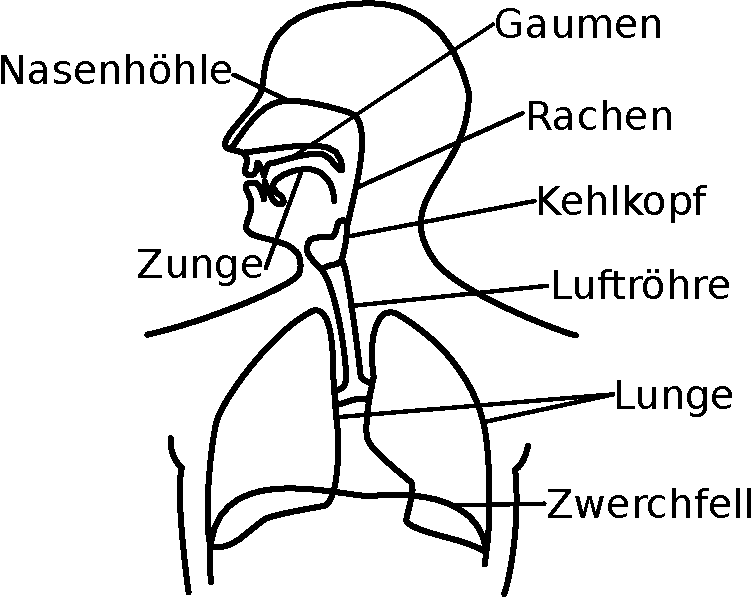
\includegraphics[width=6cm]{figures/ueberblick}
  \caption{Oberkörper und einige Organe}
  \label{fig:lunge}
\end{figure}

Das \textit{Zwerchfell} ist eine muskulöse Membran unterhalb der \textit{Lunge}, die den Herz- bzw.\ Lungenbereich von den Organen im Bauchraum trennt.
Durch Muskelanstrengung kann das Zwerchfell gesenkt werden, wodurch sich der Raum oberhalb vergrößert, wodurch wiederum ein Unterdruck relativ zur umgebenden Luft entsteht.
Durch diesen Unterdruck dehnt sich die Lunge aus, und weil sie durch die Luftröhre und den Mund- bzw.\ Nasenraum mit der umgebenden Luft verbunden ist, wird der Unterdruck mit einströmender Luft ausgeglichen (Einatmen).
Das Ausatmen ist ein passiver Vorgang, bei dem die Muskelanspannung des Zwerchfells gelöst wird, wodurch es in seine Ausgangsposition zurückkehrt und das Lungenvolumen verkleinert.
Der dabei entstehende Überdruck entweicht auf dem selben Weg, auf dem die Luft beim Einatmen eingeströmt ist.
Dieser Weg wird, wie schon erwähnt, überwiegend durch die gut zehn Zentimeter lange Luftröhre gebildet.

\TuBegin~Um diese Vorgänge nachzuvollziehen, können Sie sich direkt nach dem Ausatmen Nase und Mund zuhalten und versuchen, einzuatmen.
Sofort wird Ihnen die muskuläre Anspannung des Zwerchfells auffallen.
Außerdem wird bei zugehaltener Nase und zugehaltenem Mund das Gefühl des Unterdrucks im Brustkorb besonders auffallen, da keine Luft einströmen kann.

Dass wir diesen Luftstrom zum Sprechen benötigen, lässt sich auch leicht selber erfahren.
\TuBegin~Halten Sie die Luft an und versuchen dann, zu sprechen.
Es sollte Ihnen nicht gelingen.
Zur Kontrolle, dass Sie nicht doch atmen, hilft es, einen Spiegel dicht vor Mund und Nase zu halten.
Wenn Sie atmen, wird er beschlagen.

\subsection{Kehlkopf und Rachen}

\label{sec:kehlkopf}

Einfaches Ein- und Ausatmen verursacht zwar ein gewisses Rauschgeräusch, ist aber für viele Sprachlaute als grundlegender Mechanismus der Geräuschbildung nicht hinreichend.
Zu den vielen sprachlich relevanten Modifikationen des pulmonalen Luftstroms zählt die Benutzung des \textit{Kehlkopfes} (\textit{Larynx}).
Der Kehlkopf ist ein beweglich gelagertes System von Knorpeln.
Den vorderen, den sogenannten \textit{Schildknorpel}, kann man ertasten oder sogar sehen.
\TuBegin~Wenn Sie sich beim Sprechen vor einen Spiegel stellen oder an den Kehlkopf fassen, sehen bzw.\ merken Sie, wie er sich leicht auf und ab bewegt.

Die beiden sogenannten \textit{Stellknorpel} sind Teil des Kehlkopf-Systems.
Sie sind durch Muskelkraft kontrolliert bewegbar, und an ihnen sind die Stimmbänder aufgehängt.
Stellknorpel und Stimmbänder zusammen werden auch als die \textit{Glottis} bezeichnet.
Die relevante Funktion des Kehlkopfes aus Sicht der Phonetik ist die Produktion des \textit{Stimmtons}.
\TuBegin~Wenn Sie sich an den Kehlkopf/die Kehlkopfgegend fassen und verschiedene Wörter langsam sprechen (\zB \textit{Achat}, \textit{Verwaltungsangestellter}), werden Sie merken, dass der Kehlkopf bei einigen Segmenten (\textit{a}, \textit{w}, \textit{ng} usw.) eine Vibration produziert, bei anderen (\textit{ch}, \textit{t} usw.) aber nicht.

\index{Stimmton}
Diese Vibration ist der Stimmton.
Er entsteht dadurch, dass der pulmonale Luftstrom durch die Stimmlippen fließt, die dabei eine ganz bestimmte Spannung haben müssen.
Durch einen physikalischen Effekt (den \textit{Bernoulli-Effekt}) werden die Stimmlippen dabei dazu angeregt, in kürzesten Abständen (typischerweise mehrere hundert Mal pro Sekunde) aneinanderzuschlagen.
Diese Schläge erzeugen die charakteristische Vibration, die akustisch als Brummen oder Summen wahrgenommen wird und Sprachlaute als stimmhaft kennzeichnet.
In einem anderen, lockereren Spannungszustand vibrieren die Stimmlippen jedoch nicht, wenn Luft hindurchströmt.
\TuBegin~Sprechen Sie Wörter mit vielen \textit{h}-Segmenten am Silbenanfang aus, \zB \textit{Haha}, \textit{Hundehalter} usw.
Sie sollten bemerken dass beim \textit{h} im Kehlkopf zwar ein leichtes Rauschen entsteht, aber definitiv keinen Stimmton.

Als \textit{Rachen} (\textit{Pharynx}) bezeichnet man den Bereich zwischen Kehlkopf und Mundraum, der nach hinten durch eine relativ feste Wand begrenzt wird.
In Zusammenspiel mit der hinteren Zunge ist der Rachen in anderen Sprachen (\zB im Arabischen) an der Produktion von Segmenten beteiligt, im Standarddeutschen allerdings nicht.
\TuBegin~Ihren Rachen können Sie sehen, wenn Sie sich vor einen Spiegel stellen, die Zunge mit einem geeigneten Gegenstand herunterdrücken und \textit{ah} sagen.
Sie sehen dann geradeaus auf den oberen Rachenraum.

\subsection{Zunge, Mundraum und Nase}

\begin{figure}
  \centering
  \includegraphics[width=7cm]{figures/mundraum}
  \caption[Obere Sprechorgane und Artikulationsorte]{Obere Sprechorgane und Artikulationsorte}
  \label{fig:oberesprechorgane}
\end{figure}

Der Mundraum muss differenziert betrachtet werden, weil ein Großteil der Artikulation von Sprachlauten im Mundraum abläuft.
Eine wichtige Begrenzung des Mundraums nach unten ist die Zunge.
\TuBegin~Von Ihrer Zunge sehen Sie, wenn Sie sich vor den Spiegel stellen, nur den kleinsten Teil, nämlich den beweglichen Rücken und die bewegliche Spitze.
Der größte Teil der Zunge füllt den gesamten Bereich des Unterkiefers.
Auch hier gibt es die Möglichkeit, sich einen Eindruck davon zu verschaffen:
Fassen sie sich unter das Kinn (in den Bogen des Unterkiefers) und bewegen Sie die Zunge nach links und rechts.
Sie sollten spüren, wie sich größere muskuläre Strukturen bewegen.

Der bewegliche Teil der Zunge ist essentiell für die Bildung vieler Segmente.
Wenn wir den eigentlichen Mundraum von hinten nach vorne durchgehen, finden wir zunächst seine Begrenzung nach hinten: das \textit{Zäpfchen} (die \textit{Uvula}).
Am Zäpfchen werden tatsächlich Segmente des Deutschen gebildet, und zwar durch Anhebung des Zungenrückens.

Das \textit{Gaumensegel} (der \textit{weiche Gaumen}, das \textit{Velum}) ist ein weicher, mit Muskeln versorgter Abschnitt zwischen dem harten Gaumen und dem Zäpfchen.
\TuBegin~Man kann das Gaumensegel ertasten, indem man mit der Zunge oder einem Finger vorsichtig im Gaumen nach hinten fährt.
Während der vordere Gaumen hart ist, folgt weiter hinten eine weiche Stelle direkt vor dem Zäpfchen.
Den Zahndamm ertastet man auch sehr gut mit der Zungenspitze oder den Fingern.
Es handelt sich um die Stufe zwischen Zähnen und Gaumen.

Alle diese Teile der Mundhöhle spielen eine Rolle bei der Produktion standarddeutscher Segmente.
Eher eine indirekte Rolle bei der Sprachproduktion spielt die \textit{Nasenhöhle}.
\TuBegin~Halten Sie sich die Nase zu und sprechen Sie zunächst langanhaltend \textit{f} und \textit{s}, dann \textit{m} und \textit{n}.
Mit zugehaltener Nase sollte es nicht möglich sein, die \textit{m}- und \textit{n}-Segmente kontinuierlich auszusprechen.
Das liegt daran, dass bei diesen die Luft durch die Nasenhöhle statt durch die Mundhöhle abfließt.
Insofern ist die Nasenhöhle indirekt an der Produktion dieser Segmente beteiligt.

Zur weiteren Differenzierung des Gaumenbereichs spricht man bei der Stufe direkt hinter den Schneidezähnen vom \textit{Zahndamm} (die \textit{Alveolen}).
Außerdem sind \textit{Zähne} und \textit{Lippen} an der Sprachproduktion beteiligt, wobei hier davon ausgegangen wird, dass der Ort und die sonstige Funktion dieser Körperteile hinlänglich bekannt ist.

\section{Artikulationsart}

\label{sec:artikulationsart}

\subsection{Passiver und aktiver Artikulator}

\label{sec:artikulator}

Nachdem jetzt die an der Produktion deutscher Sprachlaute beteiligten Organe beschrieben wurden, müssen wir überlegen, wie diese Produktion genau abläuft.
Die Produktion des pulmonalen Luftstroms und des Stimmtons wurde schon beschrieben.
Im Grunde sind die einzigen Prinzipien der Produktion von Sprachlauten

\begin{enumerate}\Lf
  \item die \textit{Behinderung} (\textit{Obstruktion}) des Luftstroms, wodurch Geräusche (Zischen, Reiben, Knacken bzw.\ Knallen) entstehen, und
  \item die \textit{Veränderung von Resonanzen} der Mundhöhle durch Veränderung ihrer Form, was den Klang des Stimmtons verändert.
\end{enumerate}

Die Behinderung des Luftstroms findet an verschiedenen Stellen statt, und in diesem Zusammenhang sind zunächst die Begriffe \textit{aktiver und passiver Artikulator} zu erklären.
\TuBegin~Sprechen Sie langsam und sorgfältig das Wort \textit{Tante} und achten Sie darauf, wo sich die beweglichen Teile Ihres Mundraums jeweils befinden.
Sowohl die beiden \textit{t}-Segmente als auch die beiden \textit{n}-Segmente sind durch eine Berührung der Zunge an einer bestimmten Stelle innerhalb des Mundraums charakterisiert.
Versuchen Sie, die Stelle zu finden und anhand der Informationen aus Abschnitt~\ref{sec:anatomischegrundlagen} zu benennen, bevor Sie weiterlesen.

Beim \textit{t} und beim \textit{n} legt sich die vordere Zungenspitze gegen den Zahndamm.
Die Zunge ist dabei beweglich, der Zahndamm hingegen unbeweglich.
Dass sich zwei Körperteile auf diese Weise berühren bzw.\ annähern, ist charakteristisch für viele Artikulationen, und man nennt sie daher die \textit{Artikulatoren}.

\Definition{Artikulator}{
\label{def:artikulator}
Ein Artikulator ist ein Körperteil, der an einer Artikulation beteiligt ist.
Ein aktiver Artikulator führt dabei eine Bewegung zu einem sich nicht bewegenden passiven Artikulator aus.
\index{Artikulator}
}

Was die Artikulatoren bei welchen Segmenten genau machen, wird \textit{Artiulationsart} genannt und in den folgenden Abschnitten klassifiziert und illustriert.

\Definition{Artikulationsart}{\label{def:artart} Die Artikulationsart eines Segmentes ist die Art und Weise, in der der Luftstrom aus der Lunge durch die Artikulatoren behindert wird.}

\subsection{Stimmhaftigkeit}

\label{sec:stimmhaftigkeit}

Zunächst können wir eine grundlegende Unterscheidung in der Artikulationsart vornehmen.
In \ref{sec:kehlkopf} wurde bereits beschrieben, dass manche Segmente mit Stimmton produziert werden, aber andere nicht.
Man kann also Segmente nach ihrer \textit{Stimmhaftigkeit} unterscheiden.

\Definition{Stimmhaftigkeit}{
Ein Segment ist stimmhaft, wenn zeitgleich zu seiner primären Artikulation ein Stimmton produziert wird.
\index{Stimmhaftigkeit}
}

\subsection{Obstruenten}

Bei der zuerst zu besprechenden Gruppe von Segmenten handelt es sich um die sogenannten \textit{Obstruenten} (\textit{Geräuschlaute}, wörtlich im Latein eigentlich \textit{Hindernislaute}).
Nach der Definition folgen Abschnitte über die Unterarten von Obstruenten.

\Definition{Obstruent}{
Ein Obstruent ist ein Segment, bei dem der pulmonale Luftstrom durch eine Verengung, die die Artikulatoren herstellen, am freien Abfließen gehindert wird.
Es entstehen Geräuschlaute:
Entweder Knall- bzw.\ Knack-Laute oder Reibegeräusche durch Turbulenzen im Luftstrom.
\index{Obstruent}
}

\subsubsection{Plosive}

Bei \textit{k}-, \textit{t}- und \textit{p}-Segmenten (ähnlich \textit{g}, \textit{d}, \textit{b}) wird der Luftstrom jeweils kurz unterbrochen, und nach der Unterbrechung folgt ein deutlicher Schwall von Luft, der dann wieder abebbt.
Das liegt daran, dass die Artikulatoren einen vollständigen Verschluss des Mundraumes herstellen, der dann spontan gelöst wird.
Das entstehende Geräusch ähnelt einem Knall, und die betreffenden Segmente heißen \textit{Plosive}.
\TuBegin~Halten Sie sich eine Handfläche dicht vor den Mund und sprechen Sie folgende Wörter sorgfältig aus: \textit{Kuckuck}, \textit{Torte}, \textit{Pappe}.
Es fällt sofort auf, dass der Luftstrom nicht gleichmäßig (wie beim einfachen Atmen) aus dem Mund entweicht.

\Definition{Plosiv}{
Ein Plosiv ist ein Obstruent, bei dem einer totalen Verschlussphase eine Lösung des Verschlusses folgt und ein Knall- oder Knackgeräusch entsteht.
\index{Plosiv}
}

Plosive können wie bereits erwähnt nach Stimmhaftigkeit unterschieden werden, wie an den Wörtern \textit{danke}/\textit{tanke}, \textit{banne}/\textit{Panne}, \textit{Gabel}/\textit{Kabel} demonstriert werden kann.
Hier entsprechen jeweils \textit{d} und \textit{t}, \textit{b} und \textit{p} sowie \textit{g} und \textit{k} einem stimmhaften und einem stimmlosen Segment.

\subsubsection{Frikative}

Das Geräusch, das bei \textit{Frikativen} entsteht, kann als Rauschen (oder Reibegeräusch) beschrieben werden.
Daher kommt auch der Name, der mit \textit{Reibelaute} eingedeutscht werden kann.
\TuBegin~Sprechen und fühlen Sie folgende Wörter: \textit{Skischuhe}, \textit{Fach}, \textit{Wicht}.
Bei den Segmenten, die durch \textit{sch} (und in \textit{Ski} ausnahmsweise \textit{sk}), \textit{f}, \textit{ch} und \textit{w} wiedergegeben werden, spüren Sie ein konstantes, mehr oder weniger scharfes Entweichen von Luft.

\Definition{Frikativ}{
Ein Frikativ ist ein Obstruent, bei dem durch die Artikulatoren ein vergleichsweise enge aber nicht vollständige Verengung im Weg des pulmonalen Luftstroms hergestellt wird, wodurch dieser stark verwirbelt wird (Turbulenzen) und ein rauschendes Geräusch erzeugt wird.
\index{Frikativ}
}

Bemerkenswert ist außerdem, dass die Frikative (im Gegensatz zu den Plosiven) so lange artikuliert werden können, wie der Luftstrom aufrecht erhalten werden kann.
Die Segmente sind also \textit{kontinuierlicher} als Plosive.
Auch unter den Frikativen gibt es stimmlose und stimmhafte: \textit{sch}, \textit{ch} und \textit{f} sind stimmlos, \textit{w}-Laute aber \zB stimmhaft.
Auch das \textit{j}-Segment (\textit{Jahr}) wird oft als Frikativ artikuliert.

\subsubsection{Affrikaten}

\textit{Affrikaten} sind komplexe Segmente, nämlich eine direkte Abfolge von einem Plosiv und einem Frikativ.
Beispiele sind das \textit{ts}-Segment (orthographisch \textit{z}) in Wörtern wie \textit{Zuschauer} oder das \textit{pf}-Segment wie in \textit{Pfund}.

\Definition{Affrikate}{
\label{def:affrikate}
Eine Affrikate ist ein komplexer Obstruent aus einem Plosiv und einem folgenden Frikativ.
Der beteiligte Plosiv und der beteiligte Frikativ sind dabei \textit{homorgan} (an derselben Stelle gebildet).
\index{Affrikate}
}

Die deutschen \textit{pf}-Segmente sind \zB streng genommen nicht homorgan, wie in Abschnitt~\ref{sec:affrikatenhomorgan} diskutiert wird.
Die Frage, ob wirklich eine Affrikate oder doch zwei Segmente vorliegen, ist oft nur schwer zu entscheiden und manchmal eher eine Frage der Phonologie als der Phonetik (Abschnitt~\ref{sec:affrikaten}).

\subsection{Laterale Approximanten}

Im Deutschen ist das \textit{l}-Segment der einzige \textit{laterale Approximant}.
Dabei wird die Zungenspitze mittig an den Zahndamm gelegt, seitlich der Zunge fließt der Luftstrom aber ungehindert ab.
\TuBegin~Beobachten Sie (möglichst vor dem Spiegel), wie im Wort \textit{Ball} das letzte Segment gebildet wird.

\Definition{Lateraler Approximant}{
Ein lateraler Approximant ist ein Segment, bei dem neben einem zentralen Verschluss der Artikulatoren der Luftstrom weitgehend ungehindert ohne Bildung von Turbulenzen abfließt.
\index{Approximant}
}

\subsection{Nasale}

Wir haben bereits den Test gemacht, Wörter mit \textit{n} und \textit{m} mit zugehaltener Nase auszusprechen, und dabei festgestellt, dass dies unmöglich ist.
Bei diesen beiden Segmenten handelt es sich um \textit{Nasale}.
Bei Nasalen wird der Mundraum vollständig verschlossen, die Luft kann nirgendwohin entweichen, und die Artikulation wird unmöglich.
Dass wir verschiedene nasale Obstruenten akustisch voneinander unterscheiden können, liegt wieder an unterschiedlichen Resonanzen, genauso wie bei den Approximanten und den Vokalen (s.\ Abschnitt~\ref{sec:vokale}).

\Definition{Nasal}{
Ein Nasal ist ein Segment, bei dem durch einen vollständigen Verschluss im Mundraum (und eine Absenkung des Velums) die Luft zum Entweichen durch die Nasenhöhle gezwungen wird.
Es entstehen keine Turbulenzen.
\index{Nasal}
}

\subsection{Vokale}

\label{sec:vokale}

\textit{Vokale} werden in der Schulgrammatik gerne als \textit{Selbstlaute} bezeichnet und damit den Konsonanten als \textit{Mitlauten} gegenübergestellt.
Die Idee hinter dieser Bezeichnung ist, dass die Vokale selbständig (also für sich allein) ausgesprochen werden können, wohingegen die Konsonanten nur mit einem anderen Segment (einem Vokal) zusammen ausgesprochen werden können.
Diese Einordnung ist grundlegend falsch, da alle Konsonanten (ggf.\ nach entsprechendem phonetischen Training) selbständig realisiert werden können.
Bei Frikativen und nasalen Obstruenten ist sogar die kontinuierliche Artikulation möglich.
Da wir einen intuitiven Begriff von Vokalen haben und die orthographisch als \textit{a}, \textit{e}, \textit{i}, \textit{o}, \textit{u} sowie \textit{ä}, \textit{ö}, \textit{ü} wiedergegebenen Segmente als Vokale bereits kennen, können wir überlegen, was das Besondere an ihnen ist.
\TuBegin~Sprechen Sie sich die Vokalsegmente vor und beobachten Sie dabei (einschließlich Beobachtung im Spiegel), wie sich die Zunge, die Lippen und die sonstigen Organe im Mundraum dabei verhalten. Wenn Sie bei der Produktion von Vokalen wieder Ihren Kehlkopf ertasten, werden Sie außerdem feststellen, dass alle stimmhaft sind.

Die Zunge bewegt sich bei der Artikulation verschiedener Vokale im Mund\-raum zu verschiedenen Positionen, aber es findet bei keinem der Segmente eine deutliche Verengung an irgendeinem Artikulator statt.
Der Luftstrom kann daher weitgehend ungehindert abfließen.
Außerdem verändert sich die Formung der Lippen von rund (\zB bei \textit{u}) zu eher breit (\zB bei \textit{e}).

\Definition{Vokal}{
\label{def:vokal}
Ein Vokal ist ein Segment, bei dem der pulmonale Luftstrom weitgehend ungehindert abfließen kann, und bei dem keine geräuschhaften Anteile entstehen.
Der Klang eines Vokals wird durch eine spezifische Formung des Resonanzraumes erzeugt.
\index{Vokal}
}

Man muss an dieser Stelle wenigstens intuitiv definieren, was Resonanzen sind.
Das Phänomen, dass physikalische Körper abhängig von ihrer Form und ihrem Material einen Klang verändern, der in ihnen produziert wird, lässt sich leicht nachvollziehen.
Wenn man in ein Rohr aus Holz, in ein Metallrohr, in die hohle Hand oder in einen hohlen Betonklotz einen Ton singt, klingt dieser jeweils unterschiedlich.
Das liegt daran, dass ein Körper abhängig von seinem Material, seiner Form und Größe bestimmte Frequenzen eines Klangs verstärkt und abschwächt.
Körper haben also ein charakteristisches \textit{Resonanzverhalten} abhängig von Form und Material.
Das Resonanzverhalten des Mundraums wird nun bei Vokalen gezielt durch die Positionierung der Zunge und der Lippen verändert, denn durch die Positionierung dieser Artikulatoren ändert sich die Form des Mundraums.
Wir können also \textit{a} und \textit{i} voneinander unterscheiden, weil das Ausgangssignal des Stimmtons bei diesen Segmenten jeweils mit einem unterschiedlich geformten Mundraum zu einem anderen Klang geformt wird.

\subsection{Oberklassen für bestimmte Artikulationsarten}

\label{sec:photoberklassen}

Bei den Vokalen, Approximanten und Nasalen enthielten die Definitionen jeweils das Kriterium, dass keine Turbulenzen entstehen, während der Luftstrom abfließt.
Außerdem gibt es natürlich bei diesen Segmenten keine spontane Verschlusslösung mit Knallgeräusch wie bei den Plosiven.
Daher gibt es hier den Oberbegriff des \textit{Sonoranten}, der diese Segmente zusammenfasst und den Obstruenten gegenüberstellt.
Typisch, aber nicht notwendig für die Sonoranten ist die Stimmhaftigkeit.

\Definition{Sonoranten und Obstruenten}{
Sonoranten (Klanglaute) sind nicht-geräuschhafte Segmente, bei denen der pulmonale Luftstrom ohne Bildung von Turbulenzen durch den Mund oder die Nase abfließen kann.
Alle anderen Segmente gelten als geräuschhaft und werden Obstruenten (Geräuschlaute) genannt.
\index{Sonorant}
\index{Obstruent}
}

\Satz{Sonoranten und Stimmton}{
Sonoranten sind prototypisch stimmhaft.
}

Die Unterscheidung von Vokalen und Konsonanten hat nichts mit der Unterscheidung von Sonoranten und Obstruenten zu tun.
Die Konsonanten sind eine Sammelklasse für alle Sonoranten und Obstruenten, die keine Vokale sind.

\Definition{Konsonanten}{
Konsonanten sind alle Obstruenten, Approximanten und Nasale.
Es sind die Segmente, die typischerweise (aber nicht notwendigerweise) nicht silbisch sind, also prototypischerweise alleine keine Silbe bilden können.
\index{Konsonant}
}

Damit ergibt sich das Diagramm in \ref{fig:lautklassen} für die Klassifizierung der Segmente in der Phonetik.
In Abschnitt~\ref{sec:photpholmerkmale} werden weitere Gründe diskutiert, warum diese Klassifizierung wichtig ist.

\begin{figure}
  \centering
  \Treek[2.5]{4}{
    & \K{\textbf{Sonoranten}}\Below{(Klanglaute)}\BBel{dl}\BBel{d}\BBel{dr} &&& \K{\textbf{Obstruenten}}\Below{(Geräuschlaute)}\BBel{dl}\BBel{d}\BBel{dr} \\
    \K{\textbf{Vokale}}\Below{(silbisch)} & \K{Approximanten}\B{drr} & \K{Nasale}\B{dr} & \K{Plosive}\B{d} & \K{Frikative}\B{dl} & \K{Affrikaten}\B{dll} \\
    &&& \K{\textbf{Konsonanten}}\Below{(nicht silbisch)} \\
  }
  \caption{Grobe Klassifikation der Segmente in der Phonetik}
  \label{fig:lautklassen}
\end{figure}

\section{Artikulationsort}

\label{sec:artort}

Bisher haben wir uns darauf beschränkt, festzustellen, auf welche Art bestimmte Segmente gebildet werden.
In einigen Fällen (\zB beim \textit{l}-Segment) haben wir auch schon festgestellt, wo die Artikulatoren ggf.\ einen Verschluss oder eine Annäherung herstellen, aber das muss noch systematisch geschehen.
Dabei leitet uns Definition~\ref{def:artort}.
Gleichzeitig werden die für die Transkription des Deutschen benötigten Zeichen des weitest verbreiteten phonetischen Alphabets vorgestellt.

\Definition{Artikulationsort}{\label{def:artort} Der Artikulationsort eines Segments ist der Punkt der größten Annäherung zwischen den Artikulatoren.}

\subsection{IPA:\ Grundzeichen und Diakritika}

\index{IPA}

Das übliche phonetische Alphabet ist das der \textit{International Phonetic Association} (IPA).%
\footnote{\url{https://www.internationalphoneticassociation.org/}}	
Es basiert auf der Lateinschrift und stellt für alle in menschlichen Sprachen vorkommenden Segmente eine mögliche Schreibung zur Verfügung.
Dabei werden primäre Artikulationen in der Regel durch ein Buchstabensymbol dargestellt.
Hinzu kommen sog.\ Diakritika (Zusatzzeichen), die vor, über, unter oder neben dem Hauptzeichen geschrieben werden und genauere Informationen zur primären Artikulation kodieren.
Hier besteht also tatsächlich der Anspruch, ein System vorzulegen, in dem man so schreibt, wie man spricht (vgl.\ Abschnitt~\ref{sec:unphonetischeschreibungen}).

Es ist üblich, phonetische Transkriptionen in [~] zu schreiben, und wir übernehmen hier diese Konvention.
Man unterscheidet gemeinhin eine enge Transkription von einer weiten oder lockeren Transkription.
Bei einer engen Transkription versucht man, jedes artikulatorische Detail, das man hört, genau festzuhalten, auch die linguistisch vielleicht irrelevanten.
Bei der lockeren Transkription geht es nur darum, die wichtigen Merkmale der gehörten Segmente aufzuschreiben.
Die lockere Transkription ist prinzipiell problematisch, weil sie dazu tendiert, zu viel phonologisches Wissen in die Transkription einzubeziehen.
Eine phonetische Transkription sollte im Normalfall so beschaffen sein, dass sie genau wiedergibt, was man tatsächlich gehört hat.
Da es hier aber nur um einen ersten Einblick geht, ist unsere Transkription nicht übermäßig genau, möglichst ohne dass sich dabei verfälschende Vereinfachungen einschleichen.

\subsection{Laryngale bzw.\ Glottale}

\label{sec:photlaryngale}

\index{Laryngal}

Im Bereich des Kehlkopfs (Larynx) bzw.\ des Stimmlippensystems (Glottis) bilden Sprecher des Standarddeutschen nur zwei Segmente.%
\footnote{Für normale phonetische Belange ist die Unterscheidung von Glottis und Larynx nicht relevant, und man findet sowohl die Bezeichnung \textit{glottal} als auch \textit{laryngal}.}
Der eine ist der stimmlose laryngale Frikativ \textipa{[h]}.
In Wörtern wie \textit{Hoffenheim}, \textit{Handspiel} usw.\ kommt dieses Segment am Anfang vor.
Weiterhin ist der stimmlose laryngale Plosiv \textipa{[P]} sehr charakteristisch für das Deutsche.
\TuBegin~Wenn Sie Wörter wie \textit{Anpfiff} oder \textit{energisch} sehr deutlich und energisch aussprechen, hören Sie am Anfang des Wortes einen Plosiv, einen Knacklaut im Kehlkopf.
Er tritt auch vor dem \textit{o} in \textit{Chaot} (nicht aber in \textit{Chaos}), vor dem \textit{ei} in \textit{Verein} oder vor dem \textit{äu} in \textit{beäugen} auf.

Bei diesem bilden die Stimmlippen als aktive Artikulatoren einen Verschluss, der spontan gelöst wird.
Wenn wir das IPA-Zeichen \textipa{P} vorläufig in die normale Orthographie einfügen, ergibt sich für die obigen Wörter (\ref{ex:phot2529}).

\begin{exe}
  \ex\label{ex:phot2529}
  \begin{xlist}
    \ex{\textipa{P}Anpfiff}
    \ex{\textipa{P}energisch}
    \ex{Cha\textipa{P}ot}
    \ex{Chaos, \Ast Cha\textipa{P}os}
    \ex{Ver\textipa{P}ein}
    \ex{be\textipa{P}äugen}
  \end{xlist}
\end{exe}

Dieser laryngale Plosiv (auch \textit{Glottalverschluss}, \textit{Glottisverschluss} oder englisch \textit{glottal stop}) tritt regelhaft vor jedem vokalisch anlautenden Wort und auch vor jeder vokalisch anlautenden betonten Silbe innerhalb eines Wortes auf.
Zur Wortbetonung (dem Akzent) wird erst in Abschnitt~\ref{sec:prosodie} Substantielles gesagt.
Dort wird die Regel für die \textipa{[P]}-Einfügung weiter motiviert und illustriert.
Viele Sprachen haben einen vokalischen Anlaut ohne diesen Plosiv.
Er ist daher typisch für einen deutschen Akzent in vielen Fremdsprachen, der oft als abgehackt wahrgenommen wird.
Umgekehrt ist sein Fehlen verantwortlich dafür, dass fremdsprachliche Akzente im Deutschen von Erstsprechern des Deutschen oft als konturlos o.\,ä.\ wahrgenommen werden.

\subsection{Uvulare}

\index{Uvular}

Am Zäpfchen werden der stimmlose und der stimmhafte uvulare Frikativ gebildet: \textipa{[X]} und \textipa{[K]}.
Der stimmlose wird \textit{ch} geschrieben und tritt nur nach bestimmten Vokalen auf, also in Wörtern wie \textit{ach}, \textit{Bach}, \textit{Tuch}.%
\footnote{Die oft zu findende Behauptung, in Wörtern wie \textit{Buch} handele es sich im deutschen Standard um einen am weichen Gaumen artikulierten Velar \textipa{[x]} (s.\ Abschnitt~\ref{sec:velar}) kann ich nicht nachvollziehen.
Außer evtl.\ in Dialekten wie dem Sauerländischen findet die Artikulation gut hörbar weiter hinten im Mundraum statt, also am Zäpfchen.
}
Der stimmhafte kommt nicht bei allen Sprechern des Deutschen vor, ist aber die häufigste phonetische Realisierung von \textit{r} im Silbenanlaut, also in \textit{rot}, \textit{berauschen} usw.
\TuBegin~Zur bewussten Lokalisierung von \textipa{[X]} und \textipa{[K]}, die im hinteren Bereich der Mundhöhle gebildet werden, hilft es, die vordere Zunge mit einem geeigneten Gegenstand herunterzudrücken und dann \zB \textit{Rache} zu sagen (mit \textipa{[K]} und \textipa{[X]}).
Das klingt zwar wegen der eingeschränkten Artikulation der Vokale etwas ungewöhnlich, die Konsonanten können aber einwandfrei realisiert werden.
Hier ist zwar die Zunge der aktive Artikulator, aber nur mit dem hinteren Teil, dem Zungenrücken.

\subsection{Velare}

\label{sec:velar}

\index{Velar}

Das Velum oder Gaumensegel ist einer von mehreren Artikulationsorten, an denen im Deutschen ein stimmloser und ein stimmhafter Plosiv sowie ein Nasal artikuliert werden.
\TuBegin~Halten Sie wieder die Zungenspitze fest und artikulieren Sie \textit{King Kong} und \textit{Gang}.
Die Artikulation sollte ähnlich gut gelingen wie bei \textit{Rache}, weil auch hier die Zungenspitze nicht beteiligt ist.
Mit ein bisschen Mühe ist es möglich, den Ort und die Art der Artikulation dieser Segmente im Selbstversuch auch visuell zu beobachten.
Dazu stellt man sich vor einen Spiegel und lässt den Mund so weit wie möglich geöffnet bei der Artikulation der Beispielwörter.
Man kann dann sehen, wie sich der Zungenrücken an das Gaumensegel hebt, und wie ggf.\ der Verschluss gelöst wird.

Die \textit{k}-, \textit{g}- und \textit{ng}-Segmente werden also alle im hinteren Mundraum artikuliert, und zwar am Velum.
Der Zungenrücken ist dabei der aktive Artikulator.
Die IPA-Schreibungen sind sehr transparent: \textipa{[k]}, \textipa{[g]} und \textipa{[N]}.
Zu beachten ist, dass orthographisches \textit{ng} zumindest in der Phonetik einem Laut und nicht etwa zwei Lauten entspricht.

\subsection{Palatale}

\index{Palatal}

Am harten Gaumen finden wir im Deutschen nur das \textit{j}-Segment wie in \textit{Jahr}, \textit{Jugend} usw. und den so genannten \textit{ich}-Laut.
Das \textit{j}-Segment wird meist als palataler stimmhafter Frikativ \textipa{[J]} realisiert.
Der \textit{ich}-Laut hingegen ist immer ein palataler stimmloser Frikativ \textipa{[\c{c}]}.

\subsection{Palato-Alveolare und Alveolare}

\index{Alveolar}

Am Übergang vom harten Gaumen zum Zahndamm und am Zahndamm finden sich eine ganze Reihe von Segmenten in verschiedenen Artikulationsarten, sowohl stimmlos als auch stimmhaft.
\TuBegin~Sprechen Sie die folgenden Wörter und achten Sie auf die Anlaute: \textit{lang}, \textit{schön}, \textit{Tor}, \textit{Didi}.
Diese Segmente werden am unteren Teil des Zahndamms gebildet.
Wenn Sie in diesem Fall die Zungenspitze festhalten, können Sie diese Wörter nicht auf verständliche Weise aussprechen.

Die hier besprochenen Segmente werden im Gegensatz zu den Uvularen und Velaren mit der Zungenspitze als aktivem Artikulator gebildet.
Das \textit{l}-Segment ist der palato-alveolare laterale Approximant und wird \textipa{[l]} transkribiert.
Das \textit{sch}-Segment, bei dem meistens zusätzlich die Lippen rund geformt werden, wird \textipa{[S]} transkribiert.
Zusätzlich gibt es noch den stimmhaften palato-alveolaren Frikativ \textipa{[Z]} wie in \textit{Garage}, \textit{Marge} oder anderen, meist französischen Lehnwörtern.
Weil diese Wörter nicht zum Kernwortschatz gehören (s.\ Abschnitt~\ref{sec:kern}), lassen wir \textipa{[Z]} im weiteren Verlauf aus Übersichtstabellen usw.\ heraus.
Etwas weiter vorne werden die Anlaute folgender Wörter gesprochen, ebenfalls mit der Zungenspitze als aktivem Artikulator: \textit{Tor}, \textit{dort}, \textit{neu}, \textit{Sahne}.
Gleiches gilt für das letzte Segment in folgendem Wort: \textit{Schluss}.
Wir haben hier eine komplette Reihe von alveolarem stimmlosen Plosiv \textipa{[t]}, alveolarem stimmhaften Plosiv \textipa{[d]}, alveolarem Nasal \textipa{[n]}, alveolarem stimmhaften Frikativ \textipa{[z]} (wie in \textit{Sahne}) und alveolarem stimmlosen Frikativ \textipa{[s]} wie in \textit{Schluss}.%
\footnote{Die Segmente \textipa{[s]} und \textipa{[z]} werden dabei eigentlich etwas weiter vorne in Richtung der Zähne artikuliert.}

\subsection{Labiodentale und Bilabiale}

\index{Labial}

Im Bereich der Konsonanten sind wir von unten nach oben und hinten nach vorne durch den Vokaltrakt vorgegangen und erreichen jetzt den Bereich der Lippen.
\TuBegin~Vor dem Spiegel sieht man gleich, dass Wörter wie \textit{Pass} oder \textit{Ball} mit einem an der gleichen Stelle artikulierten Segment beginnen.
Beide Lippen (als aktive Artikulatoren) schließen sich und lösen daraufhin den Verschluss.
Es handelt sich um den stimmlosen bilabialen Plosiv \textipa{[p]} und den stimmhaften bilabialen Plosiv \textipa{[b]}.

Während bei den zuletzt genannten Segmenten beide Lippen beteiligt sind (daher der Terminus \textit{bilabial}), erkennt man bei den Anlauten von \textit{Fuß} und \textit{Wade}, dass die Zähne des Oberkiefers beteiligt sind, die sich an die Unterlippe legen.
Dort erzeugen sie keinen Verschluss sondern eine Verengung mit Reibegeräusch.
Es handelt sich daher um den stimmlosen und den stimmhaften \textit{labio-dentalen} Frikativ (\textipa{[f]} und \textipa{[v]}).

\subsection{Affrikaten und Artikulationsorte}

\label{sec:affrikatenhomorgan}

\index{Affrikate!Homorganität}

In den Wörtern \textit{Dschungel}, \textit{Chips}, \textit{Zange}, \textit{Pfanne} finden wir anlautend das gesamte Inventar der phonetischen Affrikaten im Deutschen.
Diese bestehen aus zwei aufeinanderfolgenden Phasen: einer plosiven Phase und einer frikativen Phase.
Man schreibt im IPA-Alphabet daher diese Segmente mit den Grundzeichen für den Plosiv und den Frikativ mit einem verbindenden Bogen (der \textit{Ligatur}).
Für die stimmlose palato-alveolare Affrikate wie in \textit{Matsch} schreibt man \textipa{[\t{tS}]}, für die stimmlose alveolare Affrikate wie in \textit{Zange} \textipa{[\t{ts}]} und für die stimmlose labiale Affrikate wie in \textit{Pfanne} \textipa{[\t{pf}]}.
Nur in Lehnwörtertn findet man die stimmhafte palato-alveolare Affrikate wie in \textit{Dschungel}, transkribiert \textipa{[\t{dZ}]}.

Wenn wir uns \textipa{[\t{pf}]} ansehen, stellen wir fest, dass die Bedingung der Homorganität aus Definition~\ref{def:affrikate} (S.~\pageref{def:affrikate}) strenggenommen nicht erfüllt wird, denn \textipa{[p]} ist bilabial und \textipa{[f]} labio-dental.
Insofern werden die beiden Teile der Affrikate zwar ziemlich nah beieinander gebildet, aber nicht wirklich am selben Ort.
Ohne uns in die Details dieses Problems zu vertiefen, stellen wir dies hier fest, behandeln \textipa{[\t{pf}]} aber im weiteren Verlauf als Affrikate.

\begin{table}
  \centering
  \begin{tabular}{rccccccccc}
    \lsptoprule
    \multicolumn{1}{c}{} & \Sw{\textbf{bilabial}} & \Sw{\textbf{labio-dental}} & \Sw{\textbf{alveolar}} & \Sw{\textbf{palato-alveolar}} & \Sw{\textbf{palatal}} & \Sw{\textbf{velar}} & \Sw{\textbf{uvular}} & \Sw{\textbf{laryngal}} \\
    \midrule
    \textbf{stl.\ Plosiv} & \textipa{p} & \textipa{} & \textipa{t} & \textipa{} & \textipa{} & \textipa{k} & \textipa{} & \textipa{P} \\
    \textbf{sth.\ Plosiv} & \textipa{b} & \textipa{} & \textipa{d} & \textipa{} & \textipa{} & \textipa{g} & \textipa{} & \textipa{} \\
    \textbf{stl.\ Frikativ} & \textipa{} & \textipa{f} & \textipa{s} & \textipa{S} & \textipa{\c{c}} & \textipa{} & \textipa{X} & \textipa{h} \\
    \textbf{sth.\ Frikativ} & \textipa{} & \textipa{v} & \textipa{z} & \textipa{} & \textipa{J} & \textipa{} & \textipa{K} & \textipa{} \\
    \textbf{stl.\ Affrikate} & \textipa{} & \textipa{\t{pf}} & \textipa{\t{ts}} & \textipa{\t{tS}} & \textipa{} & \textipa{} & \textipa{} & \textipa{} \\
    \textbf{sth.\ Affrikate} & \textipa{} & \textipa{} & \textipa{} & \textipa{} & \textipa{} & \textipa{} & \textipa{} & \textipa{} \\
    \textbf{lateraler Approximant} & \textipa{} & \textipa{} & \textipa{} & \textipa{l} & \textipa{} & \textipa{} & \textipa{} & \textipa{} \\
    \textbf{Nasal} & \textipa{m} & \textipa{} & \textipa{n} & \textipa{} & \textipa{} & \textipa{N} & \textipa{} & \textipa{} \\
    \lspbottomrule
  \end{tabular}
  \caption{IPA:\ Konsonanten des Deutschen}
  \label{tab:photkons}
\end{table}

\subsection{Vokale und Diphthonge}

\subsubsection{Vokale}

\index{Vokal}

Für die phonetische Klassifikation der Vokale werden in diesem Abschnitt \textit{Höhe} und \textit{Lage} als eine Art vokalischer Artikulationsort eingeführt.
Außerdem werden \textit{Rundung} und \textit{Länge} diskutiert, die strenggenommen nicht zum Artikulationsort gehören.%
\footnote{Die IPA-Symbole sind nun nahezu vollständig eingeführt und alle Beispielwörter werden ab jetzt vollständig transkribiert.}
Man fasst die Vokale normalerweise in einem sogenannten \textit{Vokalviereck} (manchmal auch \textit{Vokaltrapez} genannt) zusammen, s.\ Tabelle~\ref{tab:vokaltrap}.
Das Vokalviereck ist nichts anderes als eine Tabelle, in der die Spalten die Lage und die Zeilen die Höhe kodieren.
Wenn es eine ungerundete und eine gerundete Variante gibt, steht die gerundete stets an zweiter Stelle.
Länge wird hier nicht verzeichnet.
Der Rest dieses Abschnitts erläutert das Vokalviereck im Detail.

\index{Vokalviereck}

\begin{table}
  \centering
  \begin{tabular}{cccccc}
    \lsptoprule
    \multicolumn{1}{c}{} && \textbf{halb-} && \textbf{halb-} & \\
    \multicolumn{1}{c}{} & \textbf{vorne} & \textbf{vorne} & \textbf{zentral} & \textbf{hinten} & \textbf{hinten} \\
    \midrule
    \textbf{hoch/geschlossen} & \textipa{i y} &&&& \textipa{u} \\
    \multirow{2}{*}{\textbf{halbhoch}} && \textipa{I Y} && \textipa{U} & \\
    & \textipa{e} \textipa{\o} &&&& \textipa{o} \\
    \textbf{mittel} &&& \textipa{@} && \\
    \multirow{2}{*}{\textbf{halbtief}}& \textipa{E} \textipa{\oe} &&&& \textipa{O} \\
    &&& \textipa{5} && \\
    \textbf{tief/offen} &&& \textipa{a} && \\
    \lspbottomrule
  \end{tabular}
  \caption{IPA-Vokalviereck für das Deutsche}
  \label{tab:vokaltrap}
\end{table}

Vokale sind gewöhnlicherweise bezüglich ihres Artikulationsorts schwerer einzuordnen als Konsonanten.
Dies liegt daran, dass es für Vokale keinen gut lokalisierbaren punktuellen Artikulationsort gibt und die Orientierung im Mundraum dadurch erschwert wird.
Vielmehr wird die Zunge (sehr vereinfacht gesprochen) höher oder tiefer und weiter vorne oder weiter hinten im Mundraum lokalisiert.
Entsprechend unterscheidet man Vokale nach ihrer \textit{Lage} als \textit{vorne}, \textit{zentral} oder \textit{hinten} und ihrer \textit{Höhe} als \textit{hoch}, \textit{mittel} oder \textit{tief}.
Wenn Zwischenstufen benötigt werden, heißen diese \textit{halbvorne}, \textit{halbhinten} und \textit{halbhoch}, \textit{halbtief}.
Somit hat man auf beiden Achsen eine fünffache Unterscheidung, die insbesondere in der Phonologie ggf.\ durch elegantere Formulierungen reduziert werden kann.
Hohe Vokale kommen beispielsweise in \textit{lieb} \textipa{[li:p]}, \textit{lüg} \textipa{[ly:k]}, \textit{Trug} \textipa{[tKu:k]} vor, wobei \textipa{[i]} und \textipa{[y]} vorne liegen und \textipa{[u]} hinten.
Der tiefste Vokal ist \textipa{[a]} wie in \textit{Lab} \textipa{[la:p]}.

\index{Lippenrundung}
Weiterhin werden Vokale nach \textit{Lippenrundung} weiter unterschieden.
Der einzige Unterschied zwischen \textipa{[i]} in \textit{Liege} \textipa{[li:g@]} und \textipa{[y]} in \textit{Lüge} \textipa{[ly:g@]} oder \textipa{[e]} in \textit{Wege} \textipa{[ve:g@]} und \textipa{[\o]} in \textit{wöge} \textipa{[v\o:g@]} ist also der der Rundung.
\TuBegin~Wenn Sie wieder ein Spiegel-Experiment machen und zunächst \textit{u}, \textit{o}, \textit{ü} und \textit{ö} sprechen und dann \textit{a}, \textit{i}, \textit{e} und \textit{ä}, dann werden Sie beobachten, dass bei der Artikulation der ersten Gruppe die Lippen gerundet sind, bei der zweiten Gruppe aber nicht.

Die \textit{Länge} bezieht sich schließlich auf die Zeitdauer, für die ein Segment artikuliert wird.
Das ist nicht absolut zu verstehen, in dem Sinn, dass lange und kurze Vokal eine bestimmte Zeit von Millisekunden dauern, sondern relativ zueinander.
Es gibt von bestimmten Vokalen -- nämlich \textipa{[i]}, \textipa{[y]}, \textipa{[u]}, \textipa{[e]}, \textipa{[\o]}, \textipa{[o]} und \textipa{[a]} -- eine lange und eine kurze Variante.
Die lange Variante kommt in betonten Silben vor (\textipa{[i:]} in \textit{Liebe} \textipa{[li:b@]}, \textipa{[e:]} wie in \textit{Weg} \textipa{[ve:k]}), die kurze in unbetonten (\textipa{[i]} und \textipa{[o]} in \textit{Lithographie} \textipa{[litogKafi:]}, \textipa{[e]} wie in \textit{Methyl} \textipa{[mety:l]}).
Alle anderen Vokale sind immer kurz, auch wenn sie betont werden (\textipa{[I]} wie in \textit{Rinde} \textipa{[KInd@]}).
In Abschnitt~\ref{sec:gespanntheit} in der Phonologie wird eine Analyse der Längenverhältnisse vorgeschlagen.

\index{Schwa}
In der Tabelle findet sich schließlich noch ein besonderes Segment, nämlich das sogenannte \textit{Schwa} \textipa{[@]}.
Das Schwa ist ein \textit{Zentralvokal}, denn er steht in jeder Hinsicht in der Mitte der Vokalvierecks.
Besser ist evtl.\ die Bezeichnung \textit{Reduktionsvokal}, altertümlich hingegen \textit{Murmelvokal}.
Schwa kommt nur unbetont vor, \zB in der zweiten Silbe von Wörtern wie \textit{Tage} \textipa{[ta:g@]} oder \textit{geben} \textipa{[ge:b@n]}.
Außerdem wird (unbetontes) orthographisches \textit{-er} nach vorangehendem Konsonanten in der Liste immer als \textipa{[5]} (auch unglücklich als \textit{a-Schwa} bezeichnet) transkribiert (s.\ Abschnitt~\ref{sec:realisr}).

\subsubsection{Diphthonge}

\label{sec:diphthonge}

\index{Diphthong}

Ein \textit{Diphthong} ist etwas Ähnliches wie eine Affrikate.
Zwei Vokale werden zu einem Segment verbunden, und sie bilden dabei immer genau eine Silbe (zur Silbe mehr in Abschnitt~\ref{sec:silben}).
Es folgen einige Beispielwörter in (\ref{ex:phot2005}).

\begin{exe}
  \ex\label{ex:phot2005}
  \begin{xlist}
    \ex{\textit{Auto} \textipa{[P\t{aO}to:]}}
    \ex{\textit{keine} \textipa{[k\t{aE}n@]}}
    \ex{\textit{heute} bzw.\ \textit{Häute} \textipa{[h\t{O\oe}t@]}}
  \end{xlist}
\end{exe}

Ein häufig gemachter und wahrscheinlich von der Orthographie geleiteter Fehler sind Transkriptionen wie \textit{Auto} als \Ast\textipa{[P\t{aU}to]} oder \textit{keine} als \Ast\textipa{[k\t{aI}ne]}, obwohl die Diphthonge \textipa{[\t{aE}]} und \textipa{[\t{aO}]} eigentlich charakteristisch für den Standard und die meisten deutschen Dialekte sind.
Die Diphthonge enden auf den jeweils tieferen Vokal (\textipa{[O]} statt \textipa{[U]} und \textipa{[E]} statt \textipa{[I]}).
Es gehört sogar zum typisch deutschen Akzent in vielen Fremdsprachen (wie \zB dem Englischen), dass die Diphthonge wie im Deutschen mit abgesenktem zweiten Vokal artikuliert werden.
Im englischen \textit{buy}, \textit{scout} wird dann \textipa{[b\t{aE}]} und \textipa{[sk\t{aO}t]} statt \textipa{[b\t{aI}]} und \textipa{[sk\t{aU}t]} gesprochen.
Im Fall von \textipa{[\t{O\oe}]} wie in \textit{heute} \textipa{[h\t{O\oe}t@]} sieht man manchmal \textipa{[\t{OI}]} oder \textipa{[\t{OY}]}, was ebenfalls falsch ist.
Die Rundung des \textipa{[o]} breitet sich im Diphthong auf den zweiten Vokal aus, der deswegen nicht \textipa{[I]} sein kann.
Außerdem findet auch hier die Absenkung statt, weswegen \textipa{[\t{O\oe}]} adäquater ist als \textipa{[\t{OY}]}.

Kein Diphthong liegt dann vor, wenn lediglich zwei einzelne Vokale aufeinandertreffen.
Wenn eine Silbe auf einen Vokal endet und eine mit einem Vokal beginnende unbetonte Silbe folgt, entsteht kein Diphthong, auch wenn der Glottalverschluss nicht eingefügt wird (zum Gottalverschluss vgl.\ Abschnitt~\ref{sec:photlaryngale}).
Der Ligaturbogen darf dann in der Transkription nicht geschrieben werden.
Ein Beispiel ist \textit{Ehe} \textipa{[Pe:@]} (nicht \Ast\textipa{[P\t{e@}]}).

\section{Phonetisch-phonologische Merkmale}

\label{sec:photpholmerkmale}

Abschließend werden jetzt die phonetischen Merkmale zusammengefasst, wobei im Gegensatz zum Rest des Kapitels die Merkmalsschreibweise benutzt wird.
Dabei wird sich zeigen, dass die Organisation der Merkmale hierarchisch ist, weil bei Segmenten viele Merkmale nur dann vorhanden sind, wenn andere Merkmale bestimmte Werte haben.
Die Namen der Merkmale und Werte werden in transparenten Abkürzungen angegeben.
Für jedes Segment muss auf jeden Fall die Artikulationsart angegeben werden.

\begin{exe}
	\ex \textsc{Art}: \textit{plos}, \textit{frik}, \textit{affr}, \textit{nas}, \textit{appr}, \textit{vok}
\end{exe}

Für alle weiteren Merkmale zeigt sich, dass die Überklassen aus Abschnitt~\ref{sec:photoberklassen} nicht nur eine Konvention sind, sondern deskriptive Vorteile bringen.
Einerseits haben Konsonanten und Vokale unterschiedliche Merkmale, andererseits ist eine Spezifikation des Stimmtons nur für Obstruenten nötig.
In Kapitel~\ref{sec:phonologie} wird an einigen Stellen argumentiert werden, dass weitere Überklassen einen Erklärungsvorteil bringen, \zB die Klasse der \textit{Liquide} (\textipa{[K]} und \textipa{[l]}) in Abschnitt~\ref{sec:anfangsrandeskriptiv}.

\begin{exe}
	\ex \textbf{Vokale}
		\begin{xlist}
			\ex \textsc{Höhe}: \textit{hoch}, \textit{halbhoch}, \textit{mittel}, \textit{halbtief}, \textit{tief}
			\ex \textsc{Lage}: \textit{vorn}, \textit{halbvorn}, \textit{zentral}, \textit{halbhinten}, \textit{hinten}
			\ex \textsc{Rund}: $+$, $-$
			\ex \textsc{Lang}: $+$, $-$
		\end{xlist}
	\ex \textbf{Konsonanten}
		\begin{xlist}
			\ex \textsc{Ort}: \textit{lar}, \textit{uv}, \textit{vel}, \textit{pal}, \textit{pal-alv}, \textit{alv}
		\end{xlist}
	\ex \textbf{Obstruenten}
		\begin{xlist}
			\ex \textsc{Stimme}: $+$, $-$
		\end{xlist}
\end{exe}

Man kann das Merkmalsinventar erweitern, um die Oberklassen abzubilden.
Es käme dann (\ref{ex:phot767676}) hinzu.

\begin{exe}
	\ex{\label{ex:phot767676} \textbf{Konsonanten}}
		\begin{xlist}
			\ex \textsc{Obstruent}: $+$, $-$
		\end{xlist}
\end{exe}

Auch in der Phonologie (Kapitel~\ref{sec:phonologie}) werden in diesem Buch (mit einigen Reduktionen und Erweiterungen) die hier vorgestellten phonetischen Merkmale benutzt.
In anderen phonologischen Darstellungen (s. Literaturhinweise auf S.~\pageref{abs:pholliteratur}) wird für die Phonologie oft ein anderes Merkmalsinventar eingeführt, das sich vor allem bei den Artikulationsorten unterscheidet, weil es sich am aktiven Artikulator orientiert.
Außerdem gibt es Merkmalstheorien (sog.\ \textit{Merkmalsgeometrien}), die der hierarchischen Struktur, die hier nur angedeutet wurde, besser gerecht werden.

\section{Phonetische Transkription und Besonderheiten der Schreibung}

\label{sec:phonetischebesonderheiten}

Dieses Kapitel hat ausdrücklich keine gründliche phonetische Ausbildung zum Ziel gehabt.
Vielmehr war das weitaus bescheidenere Ziel, den Lesern einen Überblick über die Segmente zu geben, die im in Deutschland gesprochenen Standarddeutschen vorkommen.
Ein solches Vorgehen ist im Germanistikstudium üblich und durchaus gerechtfertigt. 
Transkriptionen auf Basis eines solchen Wissens sind keine Transkriptionen im eigentlichen Sinn, weil nicht Gehörtes genau notiert wird, sondern vielmehr orthographisch geschriebene Wörter in Lautschrift übersetzt werden.
Man könnte auch von \textit{Pseudo-Transkription} oder im Extremfall von \textit{Transliteration} (also von der Übersetzung einer Schrift in eine andere) sprechen.
In diesem Abschnitt werden daher einige Besonderheiten besprochen, die gerne zu Problemen bei der Pseudo-Transkription des Deutschen führen.
Dadurch wird gleichzeitig die phonetische Beschreibung weiter komplettiert und auf die Phonologie vorbereitet.

\subsection{Auslautverhärtung}

\label{sec:auslautverhaertungphonetik}

\index{Auslautverhärtung}

Bei der Transkription ist zu beachten, dass die mit den Buchstaben \textit{g}, \textit{d} und \textit{b} wiedergegebenen Segmente abhängig von ihrer Position in der Silbe nicht sie stimmhaften Plosiven \textipa{[g]}, \textipa{[d]} und \textipa{[b]} sind.
Wenn sie nämlich am Ende einer Silbe stehen, korrelieren sie mit den stimmlosen Plosiven \textipa{[k]}, \textipa{[t]} und \textipa{[p]}.
Folgen weitere Vokale (\zB in Flexionsformen), werden die Segmente aber trotzdem stimmhaft realisiert.
Die Wörter in (\ref{ex:phot7241})--(\ref{ex:phot7243}) illustrieren diesen Effekt.

\begin{exe}
  \ex\label{ex:phot7241}
  \begin{xlist}
    \ex{\label{ex:7241a} weck \textipa{[vEk]}}
    \ex{\label{ex:7241b} Weg \textipa{[ve:k]}}
    \ex{\label{ex:7241c} Weges \textipa{[ve:g@s]}}
  \end{xlist}
  \ex\label{ex:phot7242}
  \begin{xlist}
    \ex{\label{ex:7242a} bat \textipa{[ba:t]}}
    \ex{\label{ex:7242b} Bad \textipa{[ba:t]}}
    \ex{\label{ex:7242c} Bades \textipa{[ba:d@s]}}
  \end{xlist}
  \ex\label{ex:phot7243}
  \begin{xlist}
    \ex{\label{ex:7243a} Flop \textipa{[flOp]}}
    \ex{\label{ex:7243b} Lob \textipa{[lo:p]}}
    \ex{\label{ex:7243c} Lobes \textipa{[lo:b@s]}}
  \end{xlist}
\end{exe}

Man spricht bei diesem Phänomen von der \textit{Auslautverhärtung}.
Diese ist ein typischer phonologischer Prozess des Deutschen
Er wird genauso wie der Aufbau der Silbe in Kapitel~\ref{sec:phonologie} beschrieben.

\subsection{Orthographisches \textit{n}}

\label{sec:realisn}

Phonetisch ist ein mit dem Zeichen \textit{n} geschriebenes Segment nicht immer ein \textipa{[n]}.
\TuBegin~Sprechen Sie die Wörter in (\ref{ex:phot7303}) langsam aus und achten Sie auf den Artikulationsort des jeweils mit \textit{n} geschriebenen Segments.

\begin{exe}
  \ex\label{ex:phot7303}
  \begin{xlist}
    \ex{Klinke, Bank, ungenau}
    \ex{unpassend, Unbill}
    \ex{bunt, Tante, Bundestag}
  \end{xlist}
\end{exe}

Der Nasal \textipa{[n]} passt sich in seinem Artikulationsort immer an die nachfolgenden Plosive \textipa{[k]} und \textipa{[g]} an.
Wenn die bilabialen Plosive \textipa{[p]} und \textipa{[b]} folgen, hört man eine solche Anpassung nur bei manchen Sprechern.
Im Fall von \textipa{[t]} und \textipa{[d]} ist der Artikulationsort ohnehin identisch.
Es ergeben sich die Transkriptionen in (\ref{ex:phot8100}), wobei ich empfehlen würde, vor Labialen das nicht angepasste \textipa{[n]} zu transkribieren.

\begin{exe}
  \ex\label{ex:phot8100}
  \begin{xlist}
    \ex{\textipa{[klINk@]}, \textipa{[baNk]}, \textipa{[PUNg@n\t{aO}]}}
    \ex{\textipa{[PUmpas@nt]} oder \textipa{[PUnpas@nt]},\\
    	\textipa{[PUmbIl]} oder \textipa{[PUnbIl]}}
    \ex{\textipa{[bUnt]}, \textipa{[tant@]}, \textipa{[bUnd@sta:k]}}
  \end{xlist}
\end{exe}

\subsection{Silbische Nasale und silbische laterale Approximanten}

\label{sec:silbnasal}

Je nach Sprecher können auch im Standard Silben, die auf Schwa und folgenden Nasal oder Approximant enden (also \textipa{[@n]}, \textipa{[@m]} oder \textipa{[@l]}), mit einem \textit{silbischen Nasal} oder \textit{silbischen Approximanten} realisiert werden.
Dabei wird das Schwa nicht ausgesprochen, dafür aber der Nasal bzw.\ Approximant so gedehnt, dass er zusammen mit dem vorangehenden Konsonanten eine Silbe bildet.
Diese spezielle Artikulation wird durch das diakritische IPA-Zeichen \textipa{[\s{ }]} unter dem Nasal bzw.\ Approximant angezeigt.
Wenn der Nasal \textipa{[n]} silbisch wird, dann wird er normalerweise an vorangehendes \textipa{[b]} oder \textipa{[p]} in seinem Artikulationsort zu \textipa{[m]} angeglichen, ebenso an \textipa{[g]} oder \textipa{[k]} zu \textipa{[N]}, vgl.\ (\ref{ex:phot7772}).
Wir verwenden hier im weiteren Verlauf nur die Variante mit Schwa, geben aber in \ref{ex:phot7772} einige Beispiele für Wörter mit möglichen silbischen Nasalen und lateralen Approximanten.

\begin{exe}
  \ex\label{ex:phot7772}
  \begin{xlist}
    \ex{laufen \textipa{[l\t{aO}f\s{n}]} oder \textipa{[l\t{aO}f@n]}}
    \ex{haben \textipa{[hab\s{m}]} oder \textipa{[hab@n]}}
    \ex{kriegen \textipa{[kKi:g\s{N}]} oder \textipa{[kKi:g@n]}}
    \ex{rotem \textipa{[ro:t\s{m}]} oder \textipa{[ro:t@m]}}
    \ex{Mündel \textipa{[mYnd\s{l}]} oder \textipa{[mYnd@l]}}
  \end{xlist}
\end{exe}

\subsection{Orthographisches \textit{s}}

\label{sec:realiss}

Ob ein orthographisch mit \textit{s} wiedergegebenes Segment stimmlos \textipa{[s]} oder stimmhaft \textipa{[z]} ist, kann teilweise aus seiner Position im Wort abgeleitet werden.
\TuBegin~Lesen Sie die Wörter in (\ref{ex:phot1112}) laut vor und achten Sie auf die Stimmhaftigkeit der \textit{s}-Segmente.

\begin{exe}
  \ex\label{ex:phot1112}
  \begin{xlist}
    \ex{Bus, Fuß, besonders}
    \ex{Base, Straße, Basse}
    \ex{heißer, heiser}
    \ex{Sahne, Sorge}
    \ex{unser, Umsicht, also}
  \end{xlist}
\end{exe}

In der Mitte eines Wortes kommt sowohl \textipa{[z]} (\textit{Base} usw.) als auch \textipa{[s]} (\textit{Basse}) vor.
Am Wortende gibt es aber wegen der Auslautverhärtung nur stimmloses \textipa{[s]} (\textit{Bus} usw.), im Wortanlaut dafür immer nur stimmhaftes \textipa{[z]} (\textit{Sahne} usw.).
Über diese Verteilung der \textit{s}-Segmente wird in Abschnitt~\ref{sec:segmenteverteilungen} noch mehr gesagt.
Die Transkriptionen zu den Beispielen aus (\ref{ex:phot1112}) werden in (\ref{ex:phot1113}) gegeben.

\begin{exe}
  \ex\label{ex:phot1113}
  \begin{xlist}
    \ex{\textipa{[bUs]}, \textipa{[fu:s]}, \textipa{[b@zOnd5s]}}
    \ex{\textipa{[ba:z@]}, \textipa{[StKa:s@]}, \textipa{[bas@]}}
    \ex{\textipa{[h\t{aE}s5]}, \textipa{[h\t{aE}z5]}}
    \ex{\textipa{[za:n@]}, \textipa{[z\t{O@}g@]}}
    \ex{\textipa{[PUnz5]}, \textipa{[PUmzI\c{c}t]}, \textipa{[Palzo:]}}
  \end{xlist}
\end{exe}

\subsection{Korrelate von orthographischem \textit{r}}

\label{sec:realisr}
\index{r-Vokalisierung}

Dem orthographischen \textit{r} können phonetisch im Deutschen sehr viele verschiedene Segmente entsprechen, und zwar nicht nur Konsonanten.
Am Anfang einer Silbe und nach einem Konsonanten am Silbenanfang ist \textit{r} im Standard ein stimmhafter uvularer Frikativ, also \textipa{[K]}.
Beispielwörter sind \textit{Berufung} \textipa{[b@Ku:fUN]}, \textit{braun} \textipa{[bK\t{aO}n]} usw.

Am Ende einer Silbe kommt es darauf an, welcher Vokal vor \textit{r} steht.
In einer unbetonten Silbe nach Schwa verschmelzen Schwa und \textit{r} zu einem tiefen Zentralvokal \textipa{[5]} (manchmal auch unangemessenerweise a-Schwa genannt): \textit{Kinder} \textipa{[kInd5]}, \textit{Vergaser} \textipa{[f5ga:z5]} usw.
\index{Diphthong!sekundär}
Im Verbund mit anderen Vokalen entstehen sekundäre Diphthonge.
Nach \textit{a} und allen Kurzvokalen wird \textit{r} als \textipa{[@]} realisiert, und es entsteht ein Diphthong: \textit{Karneval} \textipa{[k\t{a@}n@val]} und \textit{wunderbar} \textipa{[vUnd5b\t{a@}]}.
Nach allen Langvokalen wird das \textit{r} schließlich als \textipa{[5]} im Diphthong realisiert.
Beispiele mit Langvokalen und Kurzvokalen finden sich in (\ref{ex:phot6340}).
Es werden jeweils die ungerundete und die gerundete Variante (wenn beide existieren) zusammen angegeben.

\enlargethispage{1\baselineskip}
\begin{exe}
  \ex\label{ex:phot6340}
  \begin{xlist}
    \ex{Tier \textipa{[t\t{i5}]}, Tür \textipa{[t\t{y5}]}}
    \ex{Kirche \textipa{[k\t{I@}\c{c}@]}, Bürde \textipa{[b\t{Y@}d@]}}
    \ex{nur \textipa{[n\t{u5}]}}
    \ex{Bursche \textipa{[b\t{U@}S@]}}
    \ex{der \textipa{[d\t{e5}]}, Stör \textipa{[St\t{\o5}]}}
    \ex{Chor \textipa{[k\t{o5}]}}
    \ex{gern \textipa{[g\t{E@}n]}, Börse \textipa{[b\t{\oe@}z@]}}
    \ex{Korn \textipa{[k\t{O@}n]}}
    \ex{Bar \textipa{[b\t{a@}]}}
    \ex{knarr \textipa{[kn\t{a@}]}}
  \end{xlist}
\end{exe}

Damit ergeben sich die sekundären Diphthonge wie in Tabelle~\ref{tab:sekundaerediphthonge}.
Gelegentlich werden die sekundären Diphthonge mit \textipa{[@]} als zweitem Glied auch anders beschrieben.
Manchmal wird hier ein velarer Approximant \textipa{[\textturnmrleg]} oder ein schwacher stimmhafter uvularer Frikativ \textipa{[\super K]} beschrieben.
Das sind schwer zu hörende und starken dialektalen Schwankungen unterliegende Feinheiten.
Hier wurde daher eine einheitliche Darstellung gewählt, in der das \textit{r}-Segment sowohl nach kurzen als auch nach langen Vokalen zum Vokal wird.

\begin{table}
  \centering
  \begin{tabular}{cccccc}
    \lsptoprule
    \multicolumn{1}{c}{} && \textbf{halb-} && \textbf{halb-} & \\
    \multicolumn{1}{c}{} & \textbf{vorne} & \textbf{vorne} & \textbf{zentral} & \textbf{hinten} & \textbf{hinten} \\
    \midrule
    \textbf{hoch/geschlossen} & \rnode{x1}{\textipa{i y}} &&&& \rnode{x2}{\textipa{u}} \\
    \multirow{2}{*}{\textbf{halbhoch}}&& \rnode{x3}{\textipa{I Y}} && \rnode{x4}{\textipa{U}} & \\
    & \rnode{x5}{\textipa{e \o}} &&&& \rnode{x6}{\textipa{o}} \\
    \textbf{mittel} &&& \rnode{x01}{\textipa{@}} && \\
    \multirow{2}{*}{\textbf{halbtief}}& \rnode{x7}{\textipa{E \oe}} &&&& \rnode{x8}{\textipa{O}} \\
    &&& \rnode{x00}{\textipa{5}} && \\
    \textbf{tief/offen} &&& \rnode{x9}{\textipa{a}} && \\
    \lspbottomrule
  \end{tabular}
  \ncline[nodesep=3pt]{-}{x1}{x00}
  \ncline[nodesep=3pt]{-}{x2}{x00}
  \ncline[nodesep=3pt]{-}{x3}{x01}
  \ncline[nodesep=3pt]{-}{x4}{x01}
  \ncline[nodesep=3pt]{-}{x5}{x00}
  \ncline[nodesep=3pt]{-}{x6}{x00}
  \ncline[nodesep=3pt]{-}{x7}{x01}
  \ncline[nodesep=3pt]{-}{x8}{x01}
  \nccurve[nodesep=3pt,offsetB=0.9pt]{-}{x9}{x01}
  \caption{Vokalviereck für die sekundären Diphthonge}
  \label{tab:sekundaerediphthonge}
\end{table}

\Zusammenfassung

\begin{enumerate}
  \item Schriftsystem und Lautsystem stehen in einer viel komplizierteren Beziehung, als die Aussage \textit{Man spricht es, wie man es schreibt!} suggeriert.
  \item Verschiedene Segmente kommen durch verschiedene Artikulationen (=~Obstruktionen des Luftstroms) auf dem Weg des Luftstroms von der Lunge zu den Lippen bzw. der Nase zustande.
  \item Der Stimmton unterscheidet Segmente wie \textipa{[t]} und \textipa{[d]} und wird durch das Pulsieren der Stimmlippen im Kehlkopf produziert.
  \item Die Artikulationsart beschreibt im Wesentlichen, wie stark sich der aktive Artikulator (meist die Zunge) dem passiven Artikulator (Zäpfchen, Gaumen usw.) annähert, und welche Art von Geräusch dabei zustandekommt.
  \item Der Artikulationsort ist der Punkt der größten Annäherung von aktivem und passivem Artikulator.
  \item Bei Nasalen wird der Luftstrom am Velum vollständig in die Nasenhöhle geleitet.
  \item Vokale haben keinen klar benennbaren Artikulationsort wie Konsonanten, sondern werden durch die Positionierung und Formung der Zunge bei einem allgemein sehr hohen Öffnungsgrad des Mundraums erzeugt.
  \item Es gibt phonetisch im Deutschen keine Wörter mit vokalischem Anlaut, weil immer der glottale Plosiv \textipa{[P]} eingefügt wird, \zB \textit{Anfang} \textipa{[PanfaN]}.
  \item Am Ende einer Silbe gibt es im Deutschen keine stimmhaften Plosive und Frikative.
  \item Das r-Segment wird am Silbenanfang als Frikativ ausgesprochen (\zB \textit{Beruf} \textipa{[b@Ku:f]}), am Silbenende wird er zum Vokal (\zB in \textit{Bar} \textipa{[b\t{a@}]}).
\end{enumerate}

\Uebungen

\Uebung[\onestar] \label{u31} Welche Wörter sind hier phonetisch transkribiert?

\begin{enumerate}\Lf
  \item \textipa{[Ju:b@l]}
  \item \textipa{[\t{ts}a:nP\t{a@}\t{ts}t]}
  \item \textipa{[PUnt5v\t{aE}zUN]}
  \item \textipa{[k\t{o5}]}
  \item \textipa{[li:b@sb@v\t{aE}s]}
  \item \textipa{[Pe:@bKUX]}
  \item \textipa{[SlI\c{c}t5]}
  \item \textipa{[klYN@l]}
  \item \textipa{[KUmp@lStil\t{ts}\c{c}@n]}
  \item \textipa{[baX@]}
  \item \textipa{[zi:p]}
  \item \textipa{[gl\t{aO}b@nskKi:k]}
  \item \textipa{[b\o:sP\t{a@}tI\c{c}]}
  \item \textipa{[ze:nzY\c{c}t@]}
  \item \textipa{[f5zOn@n]}
  \item \textipa{[g\t{Y@}t@l]}
\end{enumerate}

\Uebung \label{u32} Die folgenden Transkriptionen enthalten Fehler, wenn wir die in diesem Kapitel dargestellte Standardaussprache zugrundelegen.
Schreiben Sie die korrigierte IPA-Transkription auf. Beispiel: \textit{Tipp} \textipa{[tip]} $\rightarrow$ \textipa{[tIp]}

\begin{enumerate}\Lf
  \item aufgetaut \textipa{[P\t{aU}fg@t\t{aU}t]}
  \item rodeln \textipa{[ro:d@ln]}
  \item Tag \textipa{[ta:g]}
  \item umtriebig \textipa{[PUmtKI:bI\c{c}]}
  \item Wesen \textipa{[we:z@n]}
  \item Ansehen \textipa{[Panse:@n]}
  \item wenig \textipa{[ve:nIk]}
  \item kühl \textipa{[kYl]}
  \item Verein \textipa{[f5K\t{aE}n]}
  \item Spüle \textipa{[Spy:lE]}
  \item Tisch \textipa{[tIsch]}
  \item wehen \textipa{[ve:h@n]}
  \item ich \textipa{[PIX]}
  \item Lehre \textipa{[le:K5]}
  \item Quark \textipa{[qV\t{a@}k]}
\end{enumerate}

\Uebung \label{u33} Versuchen Sie, die Wörter standardkonform zu transkribieren.

\begin{enumerate}\Lf
  \item Unterschlupf
  \item niesen
  \item wissen
  \item Sachverhalt
  \item Definition
  \item Vereinshaus
  \item Kleinigkeit
  \item Sahnetorte
  \item Hustensaft
  \item ohne
  \item Bestimmung
  \item Tuch
  \item schubsen
  \item Bärchen
  \item Lobpreisung
\end{enumerate}

\chapter{Phonologie}

\label{sec:phonologie}

Die im letzten Kapitel besprochene artikulatorische Phonetik beschreibt die physiologischen Grundlagen der Sprachproduktion.
Anhand des Vorrats an Zeichen im Alphabet der IPA haben wir außerdem definiert, welche Laute im in Deutschland gesprochenen Standarddeutschen vorkommen.
Die eigentliche Frage der systematischen Grammatik bezüglich der Lautgestalt von Wörtern und größeren Einheiten ist aber, nach welchen Regularitäten diese Laute verbunden werden, und welchen Stellenwert die einzelnen Segmente und Segmentverbindungen (wie \zB Silben) im gesamten Lautsystem haben.
In der Phonologie geht es daher um das \textit{Lautsystem} und seine Regularitäten.
In Abschnitt~\ref{sec:segmentalephol} wird der Status einzelner Laute und ihrer Vorkommen behandelt.
Es wird diskutiert, wie man Laute mit Merkmalen beschreiben kann und wie Laute im Lexikon gespeichert sind.
Schließlich werden einige konkrete phonologische Strukturbedingungen des Deutschen (wie die Auslautverhärtung) systematisch dargestellt.
Dann folgt eine recht ausführliche Analyse des Silbenbaus (Abschnitt~\ref{sec:phonotaktik}).
Abschließend gibt Abschnitt~\ref{sec:prosodie} einen Einblick in die Prosodie (die Betonungslehre) und die damit in phonologische Aspekte der Wortebene.

% ==================================




\section{Segmente}

\label{sec:segmentalephol}

\subsection{Segmente, Merkmale und Verteilungen}

\label{sec:segmenteverteilungen}
\label{sec:verteilungen}

Der zentrale Begriff in der Phonologie ist zunächst wie in der Phonetik der des \textit{Segments}, vgl.\ Definition~\ref{def:segment}.
Alternativ findet man auch den Begriff des \textit{Phonems}, auf den in Abschnitt~\ref{sec:phonphonem} kurz eingegangen wird.
Allerdings geht es in der Phonologie anders als in der Phonetik um den systematischen Stellenwert der Segmente, nicht um eine reine Beschreibung ihrer Lautgestalt.
Um sich den Übergang von der Phonetik zur Phonologie klar zu machen, ist der Begriff der \textit{Verteilung} hilfreich.
Schon in Abschnitt~\ref{sec:auslautverhaertungphonetik} wurde diskutiert, dass es bestimmte Positionen im Wort und in der Silbe gibt, an denen nur bestimmte Segmente vorkommen.
Im genannten Abschnitt ging es zunächst nur um die Beschreibung verschiedener Korrelationen von Schrift und Phonetik, in der Phonologie sind solche Phänomene hingegen von hohem theoretischen Stellenwert.
Das Beispiel war die Auslautverhärtung, die dazu führt, dass in der letzten Position der Silbe Plosive immer stimmlos sind (\textit{Bad} als \textipa{[ba:t]} und nicht *\textipa{[ba:d]}).
Man muss nun aber dennoch davon ausgehen, dass die betreffenden Wörter \textit{im Prinzip} (besser: \textit{im Lexikon}) einen stimmhaften Plosiv an der entsprechenden Stelle enthalten, denn wenn (\zB in Flexionsformen) ein weiterer Vokal folgt, ist der Plosiv stimmhaft, vgl.\ \textit{Bades} \textipa{[ba:d@s] nicht *\textipa{[ba:t@s]}}.
Ausgehend von dem Begriff der phonologischen Verteilung oder Distribution kann man in der Phonologie systematisch über solche Phänomene sprechen.

\Definition{Verteilung (Distribution)}{
Die Verteilung eines Segments ist die Menge der Umgebungen, in denen es vorkommt.
\index{Verteilung}
}

Die Beschreibung der Verteilung eines Segments nimmt typischerweise Bezug auf bestimmte Positionen in der Silbe oder im Wort, oder auf Positionen vor oder nach anderen Segmenten.
Eine für das phonologische System entscheidende Frage ist, ob zwei Segmente die gleiche Verteilung oder eine teilweise oder vollständig unterschiedliche Verteilung haben.
Die Beispiele in (\ref{ex:phol6438})--(\ref{ex:phol6440}) illustrieren drei Typen von Verteilungen anhand des Vergleiches von je zwei Segmenten.
(\ref{ex:phol6438}) zeigt, dass \textipa{[t]} und \textipa{[k]} eine \textit{vollständig übereinstimmende Verteilung} haben.
Sie kommen beide am Anfang und am Ende von Silben vor.
Hingegen haben \textipa{[h]} und \textipa{[N]} eine vollständig unterschiedliche  Verteilung, wie (\ref{ex:phol6439}) zeigt.
Am Anfang einer Silbe kommt nur \textipa{[h]} vor, am Ende einer Silbe kommt nur \textipa{[N]} vor.
Schließlich demonstriert (\ref{ex:phol6440}), dass \textipa{[s]} und \textipa{[z]} eine teilweise übereinstimmende Verteilung haben.
Am Anfang der ersten Silbe eines Wortes kommt nur \textipa{[z]} vor wie in (\ref{ex:phol6440a}), am Ende der letzten Silbe eines Wortes kommt nur \textipa{[s]} vor wie in (\ref{ex:phol6440b}), und am Anfang einer Silbe in der Wortmitte kommen beide vor, \textipa{[z]} aber nur nach langem Vokal oder Diphthong wie in (\ref{ex:phol6440c}).

\begin{exe}
  \ex\label{ex:phol6438}
    \begin{xlist}
      \ex{\label{ex:phol6438a} Tot \textipa{[to:t]}, Kot \textipa{[ko:t]}}
      \ex{\label{ex:phol6438b} Schott \textipa{[SOt]}, Schock \textipa{[SOk]}}
    \end{xlist}
  \ex{\label{ex:phol6439} Hang \textipa{[haN]}, *\textipa{[Nah]}}
  \ex\label{ex:phol6440}
    \begin{xlist}
      \ex{\label{ex:phol6440a} Sog \textipa{[zo:k]}, besingen \textipa{[b@zIN@n]}, *\textipa{[so:k]}}
      \ex{\label{ex:phol6440b} fließ \textipa{[fli:s]}, \textit{Boss} \textipa{[bOs]}, *\textipa{[fli:z]}}
      \ex{\label{ex:phol6440c} heißer \textipa{[h\t{aE}s5]}, heiser \textipa{[h\t{aE}z5]}, Base \textipa{[ba:z@]}, Basse \textipa{[bas@]}, *\textipa{[baz@]}}
    \end{xlist}
\end{exe}

Wie man an den Beispielen sieht, gibt es Segmente, anhand derer Wörter (wie \textit{heißer} und \textit{heiser}) unterschieden werden können, auch wenn die Wörter ansonsten völlig gleich lauten.
Dies geht genau deswegen, weil die zwei Segmente mindestens eine teilweise übereinstimmende Verteilung haben.
Zwei Wörter, die sich nur in einem Segment unterscheiden, nennt man \textit{Minimalpaar}, und ein Minimalpaar illustriert jeweils einen \textit{phonologischen Kontrast}.

\Definition{Phonologischer Kontrast}{
\label{def:phokonseg}
Zwei phonetisch unterschiedliche Segmente bzw.\ Merkmale stehen in einem phonologischen Kontrast, wenn sie eine teilweise oder vollständig übereinstimmende Verteilung haben und dadurch einen lexikalischen bzw.\ grammatischen Unterschied markieren können.
\index{Kontrast}
}

Ein phonologischer Kontrast besteht \zB zwischen \textipa{[t]} und \textipa{[k]}, weil wir Wörter anhand dieser Segmente unterscheiden können.
Das Gleiche gilt für \textipa{[s]} und \textipa{[z]} und viele andere Paare von Segmenten.
Es gilt aber nicht für \textipa{[h]} und \textipa{[N]}, weil diese beiden Segmente keine übereinstimmende Verteilung haben, wie in (\ref{ex:phol6439}) gezeigt wurde.
Man kann mit dem Unterschied zwischen \textipa{[h]} und \textipa{[N]} als nicht zwei verschiedene Wörter unterscheiden.
Diese Art der Verteilungen nennt man komplementär.

\Definition{Komplementäre Verteilung}{
Eine komplementäre Verteilung zweier Segmente liegt dann vor, wenn die beiden Segmente in keiner gemeinsamen Umgebung vorkommen.
Komplementär verteilte Segmente können prinzipiell keinen phonologischen Kontrast markieren.
\index{Verteilung!komplementär}
}

Über Verteilungen lässt sich schon anhand des bisher eingeführten Inventars von Beispielen noch mehr sagen.
Bei der bereits besprochenen Auslautverhärtung haben wir es mit Paaren von stimmlosen und stimmhaften Plosiven zu tun, die in bestimmten Umgebungen (im Silbenanlaut) einen Kontrast markieren, der aber in anderen Umgebungen (Silbenauslaut) verschwindet.
(\ref{ex:phol-5674-1})--(\ref{ex:phol-5674-3}) zeigen dies für \textipa{[g]} und \textipa{[k]}, \textipa{[d]} und \textipa{[t]} sowie \textipa{[b]} und \textipa{[p]}.

\begin{exe}
  \ex\label{ex:phol-5674-1}
  \begin{xlist}
    \ex{Weg \textipa{[ve:k]}, Weges \textipa{[ve:g@s]}}
    \ex{Bock \textipa{[bOk]}, Bockes \textipa{[bOk@s]}}
  \end{xlist}
  \ex\label{ex:phol-5674-2}
  \begin{xlist}
    \ex{Bad \textipa{[ba:t]}, Bades \textipa{[ba:d@s]}}
    \ex{Blatt \textipa{[blat]}, Blattes \textipa{[blat@s]}}
  \end{xlist}
  \ex\label{ex:phol-5674-3}
  \begin{xlist}
    \ex{Lab \textipa{[la:p]}, Labes \textipa{[la:b@s]}}
    \ex{Depp \textipa{[dEp]}, Deppen \textipa{[dEp@n]}}
  \end{xlist}
\end{exe}

Im Silbenauslaut des Deutschen gibt es prinzipiell keinen Unterschied zwischen stimmlosen und stimmhaften Plosiven.
Solche Effekte nennt man \textit{Neutralisierungen}.

\Definition{Neutralisierung}{
Eine Neutralisierung ist die Aufhebung eines phonologischen Kontrasts in einer bestimmten Position.
\index{Neutralisierung}
}

Im Silbenauslaut wird im Deutschen also der phonologische Kontrast zwischen \textipa{[g]} und \textipa{[k]}, zwischen \textipa{[d]} und \textipa{[t]} usw.\ neutralisiert.
Allgemein gesprochen wird der Kontrast zwischen stimmlosen und stimmhaften Plosiven in dieser Position neutralisiert.
Das erklärt die Formulierung 'Zwei phonetisch unterschiedliche Segmente \textit{bzw.\ Merkmale}\ldots' in Definition~\ref{def:phokonseg}.
Phonologische Kontraste bestehen im Prinzip zwischen Merkmalen und erst in zweiter Ordnung zwischen ganzen Segmenten.

Das Feststellen von Verteilungen ist allerdings kein Selbstzweck.
Durch die Untersuchung aller Verteilungen in einer Sprache konstruiert man das phonologische System (die phonologische Komponente der Grammatik).
Dabei geht es darum, die Formen zu ermitteln, die im Lexikon gespeichert werden müssen, und die Strukturbedingungen (wie die Auslautverhärtung) zu beschreiben, an die die Segmente in diesen Formen ggf.\ angepasst werden müssen.
Die \textit{lexikalisch gespeicherten Formen} und die \textit{phonologischen Strukturbedingungen} produzieren dann die konkreten phonetischen Verteilungen an der Oberfläche.

\subsection{Zugrundeliegende Formen und Strukturbedingungen}
\label{sec:pholfeat}
\label{sec:ur}

Wir bleiben jetzt beim Beispiel der Auslautverhärtung, um die Idee von lexikalisch zugrundeliegenden Formen und phonologischen Strukturbedingungen einzuführen.
Die Auslautverhärtung hat wie erwähnt zur Folge, dass für Obstruenten im Silbenauslaut der Stimmtonkontrast neutralisiert wird, denn alle Obstruenten im Silbenauslaut sind stimmlos.
Wenn man das gesamte Paradigma der Wörter in (\ref{ex:phol-5674-1}) bis (\ref{ex:phol-5674-3}) ansieht, fällt aber dennoch ein bedeutender Unterschied auf.
In manchen Wörtern steht im Silbenauslaut ein Konsonant, der in anderen Umgebungen stimmhaft ist, wie in \textipa{[ve:k]} und \textipa{[ve:g@s]}.
In anderen Wörtern steht ein stimmloser Konsonant, der auch in diesen anderen Umgebungen stimmlos bleibt, wie in \textipa{[bOk]} und \textipa{[bOk@s]}.
Es ist daher naheliegend, anzunehmen, dass Wörter wie \textit{Weg} (oder \textit{Bad}, \textit{Lab} usw.) eine \textit{zugrundeliegende Form} haben, in der der letzte Obstruent stimmhaft ist.
Diese zugrundeliegende Form ist eine der wesentlichen Informationen, die zum \textit{lexikalischen Wort} gehören.
Vgl.\ Abschnitt~\ref{sec:wortwortform}.

Die eigentliche Grammatik stellt allerdings allgemeine Anforderungen an die Wohlgeformtheit von Strukturen, hier die \textit{phonologischen Strukturbedingungen}.
Der \textit{Prozess} der Auslautverhärtung (als Veränderung der Merkmale eines Segments) ist in diesem Sinn das Ergebnis einer Anpassung von Silben an die Strukturbedingung, dass Silben nicht auf stimmhafte Obstruenten enden können.%
\footnote{Man kann die phonologische Grammatik in Form von \textit{Prozessen} bzw.\ \textit{Regeln} (im technischen Sinne) formulieren, die Formen als Eingabematerial nehmen und modifiziert als Ausgabematerial wieder ausgeben.\index{phonologischer Prozess}
Die Auslautverhärtung wäre dann einfach als eine Regel im technischen Sinn.
Alternativ kann man davon ausgehen, dass eine phonologische Grammatik aus Beschreibungen zulässiger Strukturen besteht, an die konkrete Formen angepasst werden.
Wie diese Anpassung vor sich geht, ist auch wieder eine sehr technische Frage.
Innerhalb einer phonembasierten Theorie (Abschnitt~\ref{sec:phonphonem}) bieten sich wieder andere Möglichkeiten, die Beziehung von Formen und Strukturbedingungen zu erfassen.
Die technischen Unterschiede sind für unsere Zwecke mehr als nachrangig.
Eine deskriptive Grammatik ist wahrscheinlich am besten bedient, wenn sie sich darauf beschränkt, zu beschreiben, wie Formen im Lexikon und an der Oberfläche aussehen, also systematische Beziehungen -- eben \textit{Regularitäten} (Abschnitt~\ref{sec:regulgen}) -- feststellt.}
Man könnte umgekehrt versuchen, eine Art \textit{Anlauterweichung} anzunehmen.
Die entsprechende Strukturbedingung wäre, dass Obstruenten stimmhaften sein müssen, wenn sie im Silbenanlaut stehen.
Dann gäbe es allerdings keine Formen wie \textit{Bockes} \textipa{[bOk@s]}, sondern es würde *\textipa{[bOg@s]} herauskommen.
Die zugrundeliegende Form muss also genau die phonologischen Informationen eines Wortes enthalten, die ausreichen, um zu erklären, wie die lautliche Gestalt des Wortes in allen möglichen Formen und Umgebungen aussieht.

\Definition{Zugrundeliegende Form und Strukturbedingung}{
\label{def:pholproz}
Die zugrundeliegende Form ist eine Folge von Segmenten, die im Lexikon gespeichert wird, und auf die alle zugehörigen phonetischen Formen zurückgeführt werden können.
Die Formen werden ggf. an die phonologischen Strukturbedingungen (die Regularitäten der phonologischen Grammatik) angepasst werden.
\index{zugrundeliegende Form}
\index{Strukturbedingung}
}

Die Phonologie stellt also eine Abstraktion gegenüber der Phonetik dar.
Die Phonetik eines Wortes beschreibt nur, wie es tatsächlich ausgesprochen wird, und jedes einzelne Wort einer Sprache kann ohne Betrachtung der anderen Wörter vollständig phonetisch beschrieben werden.
Die phonologische Repräsentation eines Wortes erfordert hingegen zusätzliches Wissen um Strukturbedingungen (\zB in Form der Auslautverhärtung), um aus ihr phonetische Formen abzuleiten.
Dieses Wissen erschließt sich durch die Betrachtung des gesamten Sprachsystems, also jedes Wortes in Bezug zu allen anderen Wörtern und in allen möglichen Umgebungen.
Anders gesagt müssen die Verteilungen der Segmente und der Wörter bekannt sein.

\begin{table}
  \resizebox{\textwidth}{!}{
    \begin{tabular}{ccc}
      \lsptoprule
      \multicolumn{2}{c}{\textbf{Grammatik}} & \textbf{Externe Systeme} \\ 
      \midrule
      \textbf{Lexikon} & \textbf{Phonologie} & \textbf{Phonetik} \\
      \midrule
      /~/& $\Rightarrow$ & \textipa{[~]}\\
      zugrundeliegende Form & Anpassung an Strukturbedingungen & phonetische Realisierung \\
      \lspbottomrule
    \end{tabular}
  }
  \caption{Lexikon, Phonologie und Phonetik}
  \label{tab:pholsystem}
\end{table}

Zugrundeliegende phonologische Formen schreibt man konventionellerweise nicht in \textipa{[~]} sondern in /~/, also \zB /\textipa{ve:g}/, /\textipa{ba:d}/ und /\textipa{la:b}/.
Schematisch kann man die Verhältnisse wie in Tabelle~\ref{tab:pholsystem} darstellen.
Mit \textit{externen Systemen} sind nicht zur Grammatik gehörige Systeme wie Gehör und Sprechapparat gemeint.
Durch die unterschiedlichen Klammern (/\textipa{ba:d}/, \textipa{[ba:t]}) kann man zugrundeliegende Formen und phonetische Realisierungen in Beziehung setzen.
Im nächsten Abschnitt werden beispielhaft einige Strukturbedingungen und Verteilungen besprochen, um zu illustrieren, wie ein phonologisches System rekonstruiert werden kann.

\subsection{Strukturbedingungen und Verteilungen}

\subsubsection{Auslautverhärtung}

\label{sec:prozauslautverh}

Die Auslautverhärtung lässt sich als Strukturbedingung unter Bezug auf phonetische bzw.\ phonologische Merkmale (Abschnitt~\ref{sec:photpholmerkmale}), bestimmte Positionen in Wort oder Silbe und die Oberklassen für Segmente (Abschnitt~\ref{sec:photoberklassen}) sehr einfach und kompakt beschreiben.

\Definition{Auslautverhärtung}{[\textsc{Obstruent}:~$+$] sind [\textsc{Stimme}:~$-$] am Silbenende.}

Wenn wir zugrundeliegende Formen entsprechend an diese Bedingung anpassen wollen, muss also die Silbenstruktur bekannt sein.
Um diese geht es in Abschnitt~\ref{sec:silben} im Detail, hier werden die Silbengrenzen vorgegeben und durch Punkte markiert. 
Nur zur Veranschaulichung steht \phopro\ für \textit{wird realisiert als}.

\begin{exe}
  \ex\label{ex:phol6726}
  \begin{xlist}
    \ex{\label{ex:phol6726a} /\textipa{ba:d}/ \phopro \textipa{[ba:t]}}
    \ex{\label{ex:phol6726b} /\textipa{ba:d@s}/ \phopro \textipa{[b:ad@s]}}
    \ex{\label{ex:phol6726c} /\textipa{ba:t}/ \phopro \textipa{[ba:t]}}
  \end{xlist}
\end{exe}

Abhängig von der zugrundeliegenden Form und der Silbenstruktur muss eine Veränderung stattfinden oder nicht.
In (\ref{ex:phol6726a}) steht /\textipa{d}/ an das Silbenende, und weil /\textipa{d}/ den Wert [\textsc{Obstruent}: $+$] hat, wird der Wert des Stimmton-Merkmals auf [\textsc{Stimme}: $-$] gesetzt.
In (\ref{ex:phol6726b}) ist die Silbenstruktur anders, die Bedingung für die Auslautverhärtung ist nicht erfüllt, und die Form bleibt unverändert.
In (\ref{ex:phol6726c}) steht zwar ein Obstruent /\textipa{t}/ am Silbenende, aber es muss keine Anpassung stattfinden, weil /\textipa{t}/ von vornherein [\textsc{Stimme}: $-$] ist.

\subsection{Gespanntheit, Betonung und Länge}

\label{sec:gespanntheit}

Die Formulierung von Strukturbedingung kann helfen, die Menge der Merkmale zu reduzieren, die man zugrundeliegend spezifizieren muss.
In Abschnitt~\ref{sec:photpholmerkmale} wurde die Vokallänge als gewöhnliches Merkmal (\textsc{Lang}) eingeführt.
Gleichzeitig wurde festgestellt, dass nur die Vokale \textipa{[i y u e \o\ E o a]} lange und kurze Varianten haben.
Bezüglich der Akzentuierung bzw.\ Betonung ist ebenfalls bereits klar, dass alle Vokale bis auf \textipa{[@ 5]} betonbar sind, und dass bei den Vokalen mit Längenunterschied die Länge an die Betonung gebunden ist.
Dieser Abschnitt verfolgt zwei Ziele.
Erstens wird das Merkmal \textsc{Gespannt} vorgeschlagen, um die längbaren Vokale zusammenzufassen.
Zweitens wird dadurch das Merkmal \textsc{Lang} aus allen zugrundeliegenden Formen eliminiert und das Merkmal \textsc{Lage} wird auf drei Werte reduziert.
Für die genannten Vokale wird also zunächst das Merkmal \textsc{Gespannt} definiert.
Es ergibt sich das neue Vokalviereck in Tabelle~\ref{tab:vokalviereckmitgespannt}, das um den Preis erkauft wird, dass \textipa{[E]} und \textipa{[b]} jeweils bald gespannt, bald ungespannt gerechnet werden.

\begin{exe}
  \ex \textsc{Gespannt}: $+$, $-$
\end{exe}

\begin{table}
  \centering
  \begin{tabular}{cp{2mm}p{2mm}cp{5mm}cp{5mm}cp{5mm}cp{5mm}cp{2mm}}
   \lsptoprule
   \multicolumn{2}{c}{} & \multicolumn{5}{c}{\textbf{vorne}} & \textbf{zentral} & \multicolumn{5}{c}{\textbf{hinten}} \\
   \multirow{5}{*}{\textbf{hoch}} &&& && && && && & \\
   &&& \Dim \rnode{i}{i} &&   &&   &&   &&   &\\
   &&& \Dim \rnode{y}{y} &&  \rnode{I}{\textipa{I}} & &   & &   && \Dim \rnode{u}{u} &\\
   &&& \Dim &&  \rnode{Y}{\textipa{Y}} &&   &&  \rnode{U}{\textipa{U}} &&  \Dim &\\
   &&& \Dim &&   &&   &&   &&  \Dim &\\
\cline{8-8}
   \multirow{5}{*}{\textbf{mittel}} &&& \Dim \rnode{e}{e} &&   && \multicolumn{1}{|c|}{\textipa{@}} &&   && \Dim \rnode{o}{o} &\\
   &&& \Dim &&   && \multicolumn{1}{|c|}{}  &&   &&   &\\
   &&& \Dim \rnode{oe}{\textipa{\o}} &&  \rnode{OE}{\textipa{\oe}} && \multicolumn{1}{|c|}{\textipa{5}} &&  \rnode{O}{\textipa{O}} &&   &\\
\cline{8-8}
   &&& \Dim &&   &&   &&   &&   &\\
   &&& \Dim \rnode{E}{\textipa{E}} && \rnode{Eugs}{\textipa{E}} &&  &&   &&   &\\
   \multirow{5}{*}{\textbf{tief}} &&&  &&   &&   &&   &&   &\\
   &&&   &&   &  &  \rnode{augs}{a} & &   &&   &\\
   &&&   &&   &&   &&   &&   &\\
   &&&   &&   &&\Dim \rnode{a}{a} &&   &&   &\\
   &&& && && && && & \\
  \lspbottomrule
  \end{tabular}
  \caption{Phonologisches Vokalviereck; Grau für \textsc{Gespannt}: $+$}
  \label{tab:vokalviereckmitgespannt}
  \ncline[nodesep=3pt]{-}{i}{I}
  \ncline[nodesep=3pt]{-}{y}{Y}
  \ncline[nodesep=3pt]{-}{e}{Eugs}
  \ncline[nodesep=3pt]{-}{E}{Eugs}
  \ncline[nodesep=3pt]{-}{oe}{OE}
  \ncline[nodesep=3pt]{-}{u}{U}
  \ncline[nodesep=3pt]{-}{o}{O}
  \ncline[nodesep=3pt]{-}{a}{augs}
\end{table}

Die Vokale in den ersten Silben von \textit{Liebe} \textipa{[li:b@]}, \textit{Tüte} \textipa{[ty:t@]}, \textit{Wut} \textipa{[vu:t]}, \textit{Weg} \textipa{[ve:k]}, \textit{schön} \textipa{[S\oe:n]}, \textit{Käse} \textipa{[kE:z@]}, \textit{rot} \textipa{[ro:t]}, \textit{rate} \textipa{[Ka:t@]} gelten also gemäß dieser leicht veränderten Merkmalstheorie als \textit{gespannt}.
In diesen Beispielen sind sie betont und daher lang.
Ungespannte Vokale können zwar betont werden, aber sie werden dadurch nicht lang, \zB in \textit{Rinder} \textipa{[KInd5]}.
Formen wie *\textipa{[KI:nd5]} sind ausgeschlossen.
Man kann die Kategorie der Gespanntheit phonetisch mit einem höheren Luftdruck, erhöhter Muskelanspannung oder einer Veränderung der Position der Zungenwurzel in Verbindung bringen.
Aus Sicht der Phonologie ist der \textit{systematische} Aspekt aber wichtiger.
Für die gespannten Vokale gelten gemeinsame Strukturbedingungen, und daher sollte sie die Grammatik in jedem Fall als eine Gruppe auffassen, genauso wie die stimmhaften und stimmlosen Obstruenten usw.
Die Ablösung von der reinen phonetischen Basis rechtfertigt auch die Annahme von einem gespannten und einem ungespannten \textipa{[a]} und \textipa{[E]}, die phonetisch nicht unterscheidbar sind.
Weil die halbvorderen und halbhinteren Vokale jetzt durch die Gespanntheit von den vorderen und hinteren unterscheidbar werden, kann ein weiteres Merkmal in seinen möglichen Werten reduziert werden.

\begin{exe}
  \ex \textsc{Lage}: \textit{vorne}, \textit{zentral}, \textit{hinten}
\end{exe}

Einige Zusammenhänge sind bemerkenswert.
Je nach Auffassung, was der Kernwortschatz ist, gilt im Kernwortschatz (auf jeden Fall aber im Erbwortschatz), dass gespannte Vokale immer betont und damit immer lang sind.
Innerhalb des Kernwortschatzes gibt es damit die in Tabelle~\ref{tab:vokalviereckmitgespannt} durch Striche markierten Paare aus langen gespannten betonten und kurzen ungespannten betonten oder unbetonten Vokalen.
Während die ungespannten betont oder unbetont auftreten können, sind die gespannten immer betont.

\begin{table}
	\centering
	\begin{tabular}{clcl}
		\lsptoprule
		\textbf{gespannt} & \textbf{Beispiel} & \textbf{ungespannt} & \textbf{Beispiel} \\
		\midrule
		\textipa{[i]}  & \textit{bieten} \textipa{[bi:t@n]} & \textipa{[I]} & \textit{bitten} \textipa{[bIt@n]} \\
		\textipa{[y]}  & \textit{fühlt} \textipa{[fy:lt]} & \textipa{[Y]} & \textit{füllt} \textipa{[fYlt]} \\
		\textipa{[u]}  & \textit{Mus} \textipa{[mu:s]} & \textipa{[U]} & \textit{muss} \textipa{[mUs]} \\
		\textipa{[e]}  & \textit{Kehle} \textipa{[ke:l@]} & \textipa{[E]} & \textit{Kelle} \textipa{[kEl@]} \\
		\textipa{[E]}  & \textit{stähle} \textipa{[StE:l@]} & \textipa{[E]} & \textit{Stelle} \textipa{[StEl@]} \\
		\textipa{[\o]} & \textit{Höhle} \textipa{[h\o:l@]} & \textipa{[\oe]} & \textit{Hölle} \textipa{[h\oe l@]} \\
		\textipa{[o]}  & \textit{Ofen} \textipa{[o:f@n]} & \textipa{[O]} & \textit{offen} \textipa{[Of@n]} \\
		\textipa{[a]}  & \textit{Wahn} \textipa{[va:n]} & \textipa{[a]} & \textit{wann} \textipa{[van]} \\
		\lspbottomrule
	\end{tabular}	
  \caption{Gespannte und ungespannte Vokale im Kernwortschatz}
  \label{tab:gespungesp}
\end{table}

\Satz{Gespanntheit im Kernwortschatz}{Im Kernwortschatz sind gespannte Vokale immer betont und lang.
Zu jedem gespannten Vokal gibt es einen ungespannten.
Der ungespannte ist betont oder unbetont, aber auf jeden Fall immer kurz.}

Im erweiterten Wortschatz, der mehr Vielsilbler enthält, gilt die eingangs erwähnte Strukturbedingung, dass bei den gespannten Vokalen die Betonung die Länge kontrolliert.
Beispiele für kurze unbetonte gespannte Vokale sind \textipa{[o]} und \textipa{[i]} in der jeweils ersten Silbe der Wörter \textit{Politik} \textipa{[politIk]} (bei manchen Sprechern \textipa{[politi:k]}), die \textipa{[o]}-Segmente in \textit{Phonologie} \textipa{[fonologi:]} und \textipa{[e]} in \textit{Methyl} \textipa{[mety:l]}.
Weil diese Wörter im alltäglichen Gebrauch durchaus häufig vorkommen, wird hier nicht von \textit{peripherem Wortschatz}, sondern vorsichtiger vom \textit{erweiterten Wortschatz} gesprochen.

\Satz{Gespanntheit im erweiterten Wortschatz}{Im erweiterten Wortschatz sind gespannte Vokale lang, wenn sie betont sind und kurz, wenn sie unbetont sind.
Es gibt keine ungespannten langen Vokale.}

Völlig außerhalb dieses Systems steht übrigens das Schwa und seine Variante \textipa{[5]}.

\Satz{Schwa}{Schwa ist immer kurz und nie betont.}

Damit müssen zugrundeliegenden Formen genau wie bei der Auslautverhärtung gemäß der neu eingeführten Strukturbedingungen angepasst werden.
Man erhält zum Beispiel (\ref{ex:phol013}).

\begin{exe}
  \ex\label{ex:phol013} \begin{xlist}
  	\ex /\textipa{veg}/ \phopro \textipa{[ve:g]}
  	\ex /\textipa{h\o l@}/ \phopro \textipa{[h\o:l@]} 
  	\ex /\textipa{of@n}/ \phopro \textipa{[o:f@n]}
  \end{xlist}
\end{exe}


\subsubsection{Verteilung von [ç] und [χ]}

\label{sec:prozichach}

Die sogenannten \textit{ich}- und \textit{ach}-Segmente sind komplementär verteilt.
Es gibt kein Wort, in dem sie einen lexikalischen Unterschied markieren können.
Einige Beispielwörter, in denen \textipa{[\c{c}]} (\ref{ex:phol6110a}) und \textipa{[X]} (\ref{ex:phol6110b}) vorkommen, illustrieren dies.

\begin{exe}
  \ex\label{ex:phol6110}
  \begin{xlist}
    \ex{\label{ex:phol6110a} rieche, Bücher, schlich, Gerüche, Wehwehchen, röche, schlecht, Löcher}
    \ex{\label{ex:phol6110b} Tuch, Geruch, hoch, Loch, Schmach, Bach.}
  \end{xlist}
\end{exe}

Ausschlaggebend für das Vorkommen von \textipa{[\c{c}]} und \textipa{[X]} ist der unmittelbar vorangehende Kontext.
Nach /\textipa{i:}/, /\textipa{y:}/, /\textipa{I}/, /\textipa{Y}/, /\textipa{e:}/, /\textipa{\o}/, /\textipa{E:}/, /\textipa{E}/, /\textipa{\oe}/ kommt \textipa{[\c{c}]} vor, nach /\textipa{u:}/, /\textipa{U}/, /\textipa{o:}/, /\textipa{O}/, /\textipa{a:}/ und /\textipa{a}/ hingegen \textipa{[X]} (nach Schwa kommt keins der beiden Segmente vor).
Ein Blick auf das Vokalviereck (Abbildung~\ref{fig:vokaltrapatr}, S.~\pageref{fig:vokaltrapatr}) zeigt sofort, was der relevante Merkmalsunterschied ist.
Nach Vokalen, die [\textsc{Hinten}: $-$] sind, steht \textipa{[\c{c}]}, nach Vokalen, die [\textsc{Hinten}: $+$] sind, steht hingegen \textipa{[X]}.
Die relevanten Merkmale der beiden Frikative sind die in (\ref{ex:phol1190}).

\begin{exe}
  \ex\label{ex:phol1190}
  \begin{xlist}
    \ex{\textipa{[\c{c}]} $=$ [\textsc{Kons}: $+$, \textsc{Appr}: $-$, \textsc{Son}: $-$, \textsc{Kont}: $+$, \textsc{Ort}: \textit{dor}, \textsc{Hinten}: $-$]}
    \ex{\textipa{[X]} $=$ [\textsc{Kons}: $+$, \textsc{Appr}: $-$, \textsc{Son}: $-$, \textsc{Kont}: $+$, \textsc{Ort}: \textit{dor}, \textsc{Hinten}: $+$]}
  \end{xlist}
\end{exe}

Hier wird ein Vorteil der zunächst vielleicht etwas umständlich wirkenden phonologischen Merkmale deutlich.
Dank des sowohl vokalischen als auch konsonantischen Merkmals \textsc{Hinten} kann die Frage der Realisierung von \textipa{[\c{c}]} und \textipa{[X]} als Prozess beschrieben werden, der den Wert des Merkmals \textsc{Hinten} beim Frikativ an den entsprechenden Wert des vorangehenden Vokals angleicht bzw.\ assimiliert.
Assimilation heißt hier nichts anderes, als dass der Wert eines Merkmals mit dem eines anderen gleichgesetzt wird, was durch eine Variable (hier \textit{x}) angezeigt werden kann.
Alle Merkmale, über die auf der rechten Seite keine Angaben gemacht werden, bleiben wie sie sind.

\PholProz{\textsc{Hinten}-Assimilation (HA)}{\index{hinten!Assimilation}
[\textsc{Son}: $-$, \textsc{Kont}: $+$, \textsc{Ort}: \textit{dor}] \PhPr{HA} [\textsc{Hinten}: \textit{x}]\\
nach [\textsc{Kons}:$-$, \textsc{Hinten}: \textit{x}]
}

Es muss jetzt nur noch entschieden werden, ob in der zugrundeliegenden Form für \textipa{[\c{c}]} und \textipa{[X]} gar kein Wert für \textsc{Hinten} gespeichert ist, oder ob vielleicht einer der beiden möglichen Werte ($+$ oder $-$) zugrundeliegt und in einem der beiden Fälle geändert wird.
Aufschlussreich ist hier die Betrachtung von Wörtern wie \textit{Milch} /\textipa{mIl\c{c}}/, \textit{Storch} /\textipa{StOK\c{c}}/ oder \textit{Röckchen} /\textipa{K\oe k\c{c}@n}/, in denen \textipa{[\c{c}]} (aber niemals \textipa{[X]}) nach einem Konsonanten vorkommt.
Es ist also besser, anzunehmen, dass /\textipa{\c{c}}/ zugrundeliegt und \textipa{[X]} das phonetische Resultat einer Assimilation ist.
Aus diesem Grund wurde in Abschnitt~\ref{sec:konsonantenmerkmale} das Segment \textipa{[X]} auch nicht in /~/ gesetzt.
Es ist kein zugrundeliegendes Segment.
Damit ergeben sich die Anwendungen des Prozesses wie in (\ref{ex:phol8011}).

\begin{exe}
  \ex\label{ex:phol8011}
  \begin{xlist}
    \ex{/\textipa{I\c{c}}/ \PhPr{HA} \textipa{[PI\c{c}]}}
    \ex{/\textipa{a\c{c}}/ \PhPr{HA} \textipa{[PaX]}}
  \end{xlist}
\end{exe}

\subsection{Frikativierung von /g/}

\label{sec:prozgfrik}

Im Standard wird /\textipa{Ig}/ als \textipa{[I\c{c}.]} realisiert.
Das /\textipa{g}/ wird also zum Frikativ, und kein anderer Vokal außer /\textipa{I}/ hat diese Wirkung auf das /\textipa{g}/.
Der Prozess wird als /\textipa{g}/-Frikativierung oder /\textipa{g}/-Spirantisierung bezeichnet.
In (\ref{ex:phol8482}) sind die einzigen Merkmale von /\textipa{g}/ und /\textipa{\c{c}}/ gegenübergestellt, die sich in ihren Werten unterscheiden.

\begin{exe}
  \ex\label{ex:phol8482}
  \begin{xlist}
    \ex{/\textipa{g}/ $=$ [\textsc{Kont}: $-$, \textsc{Stimme}: $+$]}
    \ex{/\textipa{\c{c}}/ $=$ [\textsc{Kont}: $+$, \textsc{Stimme}: $-$]}
  \end{xlist}
\end{exe}

Die Änderung dieser Werte ist offensichtlich nicht gut als Assimilation an die Merkmale von /\textipa{I}/ zu beschreiben.
Der Prozess hat vielmehr etwas Willkürliches an sich.
Daher können wir ihn auch unter Bezugnahme auf ganze Segmente formulieren und müssen diese nicht unbedingt in Merkmale aufschlüsseln.%
\footnote{Man kann den Verlust der Stimmhaftigkeit auch der Auslautverhärtung überlassen.
Dies hat aber weitere Implikationen bezüglich der Reihenfolge, in der die Prozesse stattfinden müssen, weswegen dies hier nicht besprochen wird.}

\PholProz{/g/-Frikativierung (GF)}{\textipa{Ig} \PhPr{GF} \textipa{I\c{c}} in Coda}

Die Formulierung des Prozesses enthält eine wichtige Einschränkung, nämlich dass der Prozess nur am Silbenende stattfindet.
In (\ref{ex:phol9990}) sind einige Beispiele angegeben, in denen diese Einschränkung zusammen mit dem Silbifizierungsprozess interessante Resultate erzeugt.

\begin{exe}
  \ex\label{ex:phol9990}
  \begin{xlist}
    \ex{/\textipa{ve:nIg}/ \PhPr{SI} \textipa{[.ve:.nIg.]} \PhPr{GF} \textipa{[.ve:.nI\c{c}.]}}
    \ex{/\textipa{ve:nIg@}/ \PhPr{SI} \textipa{[.ve:.nI.g@.]} \PhPr{GF} \textipa{[.ve:.nI.g@.]}}
  \end{xlist}
\end{exe}

Wie schon bei der Auslautverhärtung (Abschnitt~\ref{sec:prozauslautverh}) kann die Silbifizierung die Anwendbarkeit anderer Prozesse beeinflussen.
Weil im Wort \textit{wenige} das /\textipa{g}/ in den Onset der letzten Silbe gerät (und nicht in die Coda wie bei \textit{wenig}), kann die \textit{g}-Frikativierung nicht eintreten, denn sie ist beschränkt auf die Codaposition.

\subsection{/ʁ/-Vokalisierungen}

\label{sec:prozrvok}

Mit der Diskussion der /\textipa{K}/-Vo\-ka\-li\-sie\-rung (RV) schließt jetzt der Abschnitt über die phonologischen Prozesse.
In Abschnitt~\ref{sec:realisr} wurden verschiedene phonetische Korrelate von geschriebenem \textit{r} besprochen.
Die Schrift ist hier eigentlich besonders systematisch, denn orthographisches \textit{r} entspricht immer einem zugrundeliegenden /\textipa{K}/ (vgl.\ auch Abschnitt~\ref{sec:buchstabensegmente}).
In (\ref{ex:phol9906}) sind einige Beispiele zusammengestellt, die dies illustrieren.

\begin{exe}
  \ex\label{ex:phol9906}
  \begin{xlist}
    \ex{geringer \textipa{[.g@.KIN.5.]}, geringere \textipa{[.g@.KIN.@.K@.]}}
    \ex{Bär \textipa{[.b\t{E5}.]}, Bären \textipa{[.bE:.K@n.]}}
    \ex{knarr \textipa{[.kn\t{a@}.]}, knarre \textipa{[.kna.K@.]}}
  \end{xlist}
\end{exe}

Wenn ein zugrundeliegendes /\textipa{K}/ im Onset steht, wird es als konsonantisches \textipa{[K]} realisiert.
Demgegenüber müssen für /\textipa{K}/ in Codas drei Fälle unterschieden werden.
Erstens gibt es eine dem Schwa ähnliche Realisierung von /\textipa{@K}/, nämlich \textipa{[5]}.
Dieses steht niemals in einer akzentuierten Silbe, da Schwa niemals in solchen Silben vorkommt.
Bei allen anderen Vokalen muss zwischen langen und kurzen Vokalen unterschieden werden.
Ein langer Vokal vor /\textipa{K}/ verliert an Länge, und das /\textipa{K}/ wird als \textipa{[5]} realisiert.
Nach kurzem Vokal wird /\textipa{K}/ schließlich als \textipa{[@]} realisiert.
Wegen der komplizierten Verhältnisse versuchen wir im Fall der /\textipa{K}/-Vokalisierung nicht, den Prozess vollständig mit Merkmalen zu beschreiben und geben einfach die drei möglichen Varianten an.

\PholProz{/ʁ/-Vokalisierung}{\index{r-Vokalisierung}
\begin{tabular}{ccc}
  \textipa{@K} & \PhPr{RV} & \textipa{5} am Silbenende\\
  {}\textipa{K} & \PhPr{RV} & \textipa{5} nach [\textsc{Lang}: $+$] am Silbenende\\
  {}\textipa{K} & \PhPr{RV} & \textipa{@} nach [\textsc{Lang}: $-$] am Silbenende
\end{tabular}
}

Interessant ist, dass in allen diesen Fällen die Coda der Silbe letztendlich nicht besetzt wird, sondern im Nukleus ein sekundärer Diphthong entsteht.
Der Begriff des sekundären Diphthongs wurde in Abschnitt~\ref{sec:realisr} bereits benutzt, jetzt können wir genauer angeben, was darunter zu verstehen ist.
Es handelt sich um Diphthonge, die auf die Vokalisierung eines zugrundeliegenden Konsonanten zurückgehen.

%\subsection{Affrikaten}
%
%\label{sec:affrikaten}
%
%\textbf{?? ERWEITERN, INTEGRATION PRÜFEN}
%
%Die Affrikaten sind hier aus Platzgründen weitgehend aus der Diskussion ausgespart worden.
%Eine wichtige Frage ist allerdings, ob in der Phonologie Affrikaten wie \textipa{[\t{ts}]} als ein Segment behandelt werden sollen, oder als eine Folge aus zwei Segmenten (hier \textipa{[t]} und \textipa{[s]}).
%Der Weg zur Lösung dieser Frage führt über die Verteilung der Affrikaten.
%Wenn Fremdwörter (bzw.\ Wörter jenseits des Kernwortschatzes, vgl.\ Abschnitt~\ref{sec:nichtkernschreib}) einmal ausgeklammert werden (\zB \textit{Chips} oder \textit{tschechisch}), ergibt sich ein interessantes Bild für die drei primären Kandidaten für Affrikaten.
%Vgl.\ dazu die Beispiele in (\ref{ex:phol81209}).
%
%\begin{exe}
%  \ex\label{ex:phol81209} 
%  \begin{xlist}
%    \ex{\label{ex:phol81209a} Zange, Platz}
%    \ex{\label{ex:phol81209b} Pfund, Napf}
%    \ex{\label{ex:phol81209c} --, Matsch}
%  \end{xlist}
%\end{exe}
%
%Während /\textipa{\t{ts}}/ und /\textipa{\t{pf}}/ im Onset und in der Coda von Silben vorkommen können, kann /\textipa{\t{tS}}/ nur im Auslaut vorkommen.
%Weil sich /\textipa{\t{ts}}/ und /\textipa{\t{pf}}/ also verteilen wie andere stimmlose Obstruenten, kann man sie parallel zu diesen als ein Segment behandeln, aber /\textipa{\t{tS}}/ eher nicht.
%
%Bei /\textipa{\t{pf}}/ kommt hinzu, dass das /\textipa{f}/ als einzelnes Segment in dieser Position eine weitere Verletzung des Sonoritätskontur mit sich brächte.
%Durch die Auffassung, dass /\textipa{\t{pf}}/ zusammen ein Segment darstellt, verhindert man dies.
%
%




% ==================================




\section{Silben und Wörter}

\label{sec:phonotaktik}

\subsection{Phonotaktik}

Aufbauend auf die Beschreibung der einzelnen Segmente des Deutschen (Kapitel~\ref{sec:phonetik}) kann und sollte beschrieben werden, wie diese Segmente zu größeren Einheiten zusammengesetzt werden, wie also \textit{phonologische Struktur} (zum Strukturbegriff vgl.\ Abschnitt~\ref{sec:strukturen}, S.~\pageref{sec:strukturen}) aufgebaut wird.
Die Wörter in (\ref{ex:phol2852}) sind Phantasiewörter in Standardorthographie und hypothetischer phonetischer Umschrift.

\begin{exe}
  \ex\label{ex:phol2852}
  \begin{xlist}
    \ex{\label{ex:phol2852a} Nka \textipa{[Nka:]}, Totk \textipa{[tOtk]}, Pkafkme \textipa{[pkafkm@]}}
    \ex{\label{ex:phol2852b} Klie \textipa{[kli:]}, Filb \textipa{[fIlp]}, Renge \textipa{[KEN@]}}
  \end{xlist}
\end{exe}

Die hypothetischen Wörter in (\ref{ex:phol2852a}) unterscheiden sich deutlich von denen in (\ref{ex:phol2852b}).
Während die zweite Gruppe nämlich zumindest mögliche Wörter des Deutschen darstellt, enthält die erste Gruppe nur Wörter, die aus irgendeinem Grund niemals Wörter des Gegenwartsdeutschen sein könnten.
Der Grund dafür ist, dass die erste Gruppe \textit{phonotaktisch nicht wohlgeformte Wörter} enthält.
Es muss also Regularitäten geben, nach denen sich Segmente des Deutschen zu größeren Einheiten wie Silben und Wörtern zusammensetzen.

\Definition{Phonotaktik}{
Die Phonotaktik beschreibt die Regularitäten, nach denen Segmente zu größeren Strukturen zusammengesetzt werden.
Die Phonotaktik definiert Einheiten wie die \textit{Silbe} und das \textit{Wort}.
\index{Phonotaktik}
}

Die Silbe ist die Einheit, mittels derer die meisten Einschränkungen für mögliche Segmentfolgen formuliert werden können.
Dieser Abschnitt ist daher ausschließlich der Silbe gewidmet.

\subsection{Silben}

\label{sec:silben}

\index{Silbe}

Was Silben genau sind, ist nicht unbedingt leicht zu definieren.
Sie sind intuitiv Einheiten, die größer sein können (aber nicht müssen) als Segmente, aber kleiner sein können (nicht müssen) als Wörter.
Der Extremfall, bei dem Segment, Silbe und Wort zusammenfallen, ist im Deutschen nur möglich, wenn man den Glottalverschluss ignoriert (s.~\ref{sec:glottalverschluss}).
Selbst dann ist dieser Fall im Deutschen im normalen Wortschatz marginal und auf Interjektionen (Rufwörter) wie \textit{oh} \textipa{[Po:]} und \textit{ah} \textipa{[Pa:]} beschränkt.
Wenn man Diphthonge als ein Segment zählt, kommt das Substantiv \textit{Ei} \textipa{[P\t{aE}]} hinzu.
Auch in anderen Sprachen ist dieser Fall eher selten, vergleiche französische Substantive wie \textit{œufs} \textipa{[\o:]} `Eier' (nur im Plural) oder \textit{eau} \textipa{[o:]} `Wasser' sowie das schwedische Substantiv \textit{ö} \textipa{[\o:]} `Insel' (nur im Singular), die insgesamt auch innerhalb ihrer eigenen Sprachsysteme eher Exoten darstellen.%
\footnote{Auf jeden Fall entfällt in diesen Sprachen aber der Glottalverschluss.} 
Meistens bestehen Silben aus mehreren Segmenten, und Wörter bestehen häufig aus mehreren Silben.
Beispiele für einsilbige Wörter aus zwei Segmenten im Deutschen sind \textit{Schuh} \textipa{[Su:]} oder \textit{Tee} \textipa{[te:]}, Beispiele für zweisilbige Wörter aus zweisegmentigen Silben sind \textit{Tüte} \textipa{[ty:t@]} oder \textit{rege} \textipa{[Ke:g@]}.
Ein einsilbiges Wort mit deutlich mehr als zwei Segmenten ist \textit{Strauch} \textipa{[StK\t{aO}X]}. 
Die wesentliche Frage der Silbenphonologie wird sein, wie hoch die Komplexität solcher Strukturen maximal sein kann.

\index{Silbe!Klatschmethode}

In der Grundschuldidaktik wird oft über die \textit{Klatschmethode} versucht, Kindern ein Gefühl für Silben zu vermitteln.
Dabei wird gesagt, dass jedes Stück eines Wortes, zu dem man bei abgehacktem Sprechen einmal klatschen kann, eine Silbe sei.
Diese Methode ist problematisch, da sie sehr leicht absichtlich oder unabsichtlich sabotierbar ist:
Es ist für viele Sprecher vielleicht natürlicher, auf Wörter wie \textit{Mutter} \textipa{[mUt5]} nur einmal zu klatschen, da die Silbe mit dem \textipa{[5]} unbetont und phonologisch nicht sehr prominent ist.
Außerdem wird mit der Methode meist ein rein orthographisch-didaktisches Ziel ohne jede Sensibilität für Grammatik verfolgt, nämlich das Erlernen der Silbentrennung in der Schrift.
Die Regeln der orthographischen Silbentrennung im Deutschen erfordern aber subtilere Kenntnisse grammatischer Regularitäten, als sie die Klatschmethode vermitteln kann.
Ein Kind wird durch das Klatschen vielleicht intuitiv lernen, dass Wörter wie \textit{Kriecher}, \textit{Iglu} oder \textit{Mutter} aus genau zwei Silben bestehen.
Ob die Silbentrennung aber \textit{Krie-cher} oder \textit{Kriech-er}, \textit{I-glu} oder \textit{Ig-lu} und \textit{Mutt-er}, \textit{Mut-ter} oder \textit{Mu-tter} ist, ist prinzipiell durch Klatschen nicht erlernbar.
Daher müssen Lehrer bei solchen Übungen dann unnatürliche Aussprachen vormachen, \zB \textipa{[mUt]} -- \textipa{[ta]} oder gar \textipa{[mUt]} -- \textipa{[tEK]} statt korrekt \textipa{[mUt5]}.
Gerade dieses Abhacken macht \textit{Kriech-er} aber genauso plausibel wie \textit{Krie-cher}.
In Fall der zerhackten Aussprache in Fällen mit orthographischen Doppelkonsonanten wie \textipa{[mUt]} -- \textipa{[ta]} muss man zudem paradoxerweise bereits Kenntnisse der Orthographie und Silbentrennung besitzen, um das Wort überhaupt so aussprechen zu können.
Man dreht sich also im Kreis, und ein solider Lernerfolg durch das Klatschen ist daher nicht zu erwarten.%
\footnote{Aus meiner eigenen -- zugegebenermaßen länger zurückliegenden -- Grundschulerfahrung als Schüler mit zwei Lehrerinnen in zwei verschiedenen Bundesländern läuft die Unterrichtseinheit dann so ab, dass einige Kinder aus Haushalten mit hohem Bildungsniveau bereits seit längerem lesen können und die Silbentrennung durch Anschauung beim Lesen intuitiv gelernt haben.
Diese Kinder verstehen in den Augen des Lehrpersonals durch das Klatschen, wie Wörter zu trennen sind.
Alle andere Kinder gelten ohne ihr Verschulden als schwierig bzw.\ langsame Lerner.
Diese Beobachtung hat natürlich keinen Anspruch auf Allgemeingültigkeit.}

Trotz ihrer absoluten Unzulänglichkeit für den Grundschulunterricht veranschaulicht die Klatschmethode (recht umständlich) allerdings ein wichtiges Prinzip der Silbenbildung.
Silben bringen die Segmente in eine schematische Ordnung, die charakteristischen artikulatorischen Einheiten entspricht.
Diese artikulatorischen Einheiten sind Schübe, die im Prinzip einem Öffnen und Schließen des Vokaltraktes entsprechen.
An einsilbigen Wörtern wie \textit{Tag} \textipa{[ta:k]} oder \textit{gut} \textipa{[gU:t]} sieht man, dass sie mit einem Verschluss beginnen und mit einem Verschluss enden, während in der Mitte beim Vokal der Vokaltrakt geöffnet ist (genauer in Abschnitt~\ref{sec:sonoritaet}).
Im Kern der Silbe befindet sich passend dazu im Deutschen immer ein Vokal, also ein Segment bei dem sich die Artikulatoren nicht punktuell annähern (Abschnitt~\ref{sec:vokale}).
Die Klatschmethode kann man also auf die Anweisung reduzieren, bei jedem Vokal einmal zu klatschen.
Wie an den Zweifelsfällen weiter oben gezeigt wurde, löst das aber nicht das Problem, ob Konsonanten zwischen den Vokalen in mehrsilbigen Wörtern zur ersten oder zweiten Silbe gehören.

Komplizierter wird die Silbenphonologie dadurch, dass in den Formen eines Wortes die Silbengrenzen nicht konstant sind.
Anders gesagt ist die Silbenstruktur von Wörtern nicht im Lexikon festgelegt.
Die Beispiele (\ref{ex:phol1830}) zeigen dies.
In der Transkription werden die Silbengrenzen durch einen einfachen Punkt markiert.

\begin{exe}
  \ex\label{ex:phol1830}
  \begin{xlist}
    \ex{Ball \textipa{[bal]}, Bälle \textipa{[bE.l@]}}
    \ex{Knall \textipa{[knal]}, Knalls \textipa{[knals]}}
    \ex{Sturm \textipa{[St\t{U@}m]}, Stürme \textipa{[St\t{Y@}.m@]}}
    \ex{Mittelstürmer \textipa{[mI.t@l.St\t{Y@}.m5]}, Mittelstürmerin \textipa{[mI.t@l.St\t{Y@}.m@.KIn]}}
  \end{xlist}
\end{exe}

Ein Wort wie \textit{Ball} ist im Nominativ Singular einsilbig, und das \textipa{[l]} steht im Auslaut (am Ende) dieser einen Silbe.
Mit dem hinzutretenden \textipa{[@]} der Plural-Endung verändert sich auch die Silbenstruktur:
Das \textipa{[l]} steht im Anlaut (am Anfang) der zweiten Silbe.
Ähnliches passiert bei \textit{Sturm} und \textit{Stürme} mit dem \textipa{[m]}.
Bei \textit{Mittelstürmer} \textipa{[mI.t@l.St\t{Y@}.m5]} und \textit{Mittelstürmerin} \textipa{[mI.t@l.St\t{Y@}.m@.KIn]} wird es noch komplizierter, weil /\textipa{K}/ nur dann als Konsonant \textipa{[K]} realisiert wird, wenn noch ein Vokal folgt und das /\textipa{K}/ dadurch in den Silbenanlaut gerät (vgl.\ dazu genauer Abschnitt~\ref{sec:prozrvok}).
Wenn bei \textit{Ball} und \textit{Balls} aber ein \textipa{[s]} hinzutritt, bleibt das Wort einsilbig, und das \textipa{[s]} wird an die einzige Silbe hinten angehängt.
Die Silbenbildung, so wie sie hier betrachtet wird, ist also keine phonetische Fragestellung, sondern eine phonologische, weil ihre Beschreibung es erfordert, dass das Gesamtsystem (also \zB alle Formen eines Wortes) betrachtet werden.
Entsprechend wird Definition~\ref{def:silbe} gegeben.

\Definition{Silbe und Silbifizierung}{\label{def:silbe}
Silben sind die nächstgrößeren phonologischen Einheiten nach den Segmenten.
Die Segmente sind ihre kleinsten Konstituenten.
Die Silbenstruktur ist nicht im Lexikon abgelegt und wird durch einen Prozess zugewiesen (Silbifizierung).
\index{Silbe}
}

Mit Klatschen ist es also nicht getan.
Der analytische Einstieg in die Silbenstruktur des Deutschen gelingt am leichtesten über einsilbige Wörter.
Abschnitt~\ref{sec:einsilbler} leistet (nach der Einführung einiger technischer Begriffe in Abschnitt~\ref{sec:silbenstruktur}) daher zunächst eine einfache Beschreibung möglicher einsilbiger Wörter des Deutschen.
Die Verallgemeinerung zu mehrsilbigen Wörtern erfolgt nach einer theoretischen Ergänzung (Abschnitte~\ref{sec:sonoritaet}) in Abschnitt~\ref{sec:mehrsilbler}.






\subsection{Strukturformat für Silben}

\label{sec:silbenstruktur}

In diesem Abschnitt wird nur die Terminologie eingeführt, mit der man über Positionen in der Silbe redet.
Offensichtlich bilden Silben komplexere Strukturen aus, die sich um einen Vokal oder Diphthong im \textit{Kern} herum gruppieren.%
\footnote{Eine alternative Sichtweise würde bei Diphthongen das zweite Glied als Teil der Coda analysieren.
Für unsere Zwecke ist der sich ergebende theoretische Unterschied vernachlässigbar.}
Für die drei sich ergebenden Konstituenten der Silbe gibt es verschiedene Bezeichnungen, von denen hier \textit{Anfangsrand}, \textit{Kern} und \textit{Endrand} verwendet werden.
Aus Gründen, die erst in Abschnitt~\ref{sec:mehrsilbler} diskutiert werden, hat es sich als nützlich erwiesen, Kern und Endrand zu einer eigenen Konstituente, dem \textit{Reim} zusammenzufassen.
Neben Definition~\ref{def:kern} wird eine Baumdarstellung der allgemeinen Silbenstruktur in Abbildung~\ref{fig:silbenstruktur} und ein Beispiel (\textit{fremd}) in Abbildung~\ref{fig:phonstr} gegeben.

\Definition{Silbenstruktur}{
\label{def:kern}
\label{def:anfangsrand}
\label{def:endrand}
Der \textit{Silbenkern} (der \textit{Nukleus}) wird immer durch einen Vokal oder Diphthong gebildet.
Die Konsonanten vor dem Kern bilden den \textit{Anfangsrand} (den \textit{Onset}), die nach dem Kern den \textit{Endrand} (die \textit{Coda}).
Es gibt Silben mit leeren Anfangs- und\slash oder Endrändern, aber keine Silben ohne Kern.
Kern und Endrand bilden den \textit{Reim}.
\index{Silbe!Kern}
\index{Silbe!Anfangsrand}
\index{Silbe!Endrand}
\index{Silbe!Reim}
}

\begin{figure}
  \centering
  \Tree[2]{
    & \K{Silbe}\B{dl}\B{d} \\
    \K{Anfangsrand} & \K{Reim}\B{d}\B{dr} \\
    & \K{Kern} & \K{Endrand}\\
  }
  \caption{Silbenstruktur}
  \label{fig:silbenstruktur}
\end{figure}

\begin{figure}
  \centering
  \Tree[1.5]{
  & && \K{Silbe}\B{dll}\B{d} \\
  & \K{Anfangsrand}\B{ddl}\B{ddr} && \K{Reim}\B{d}\B{drr} \\
  &&& \K{Kern}\B{d} && \K{Endrand}\B{dl}\B{dr} \\
  \K{\textipa{[f]}} && \K{\textipa{[K]}} & \K{\textipa{[E]}} & \K{\textipa{[m]}} && \K{\textipa{[t]}} \\
  }
  \caption{Beispiel für Silbenstruktur}
  \label{fig:phonstr}
\end{figure}








\subsection{Einsilbler}

\label{sec:einsilbler}

In diesem Abschnitt werden einsilbige Wörter herangezogen, um die minimale und die maximale Komplexität deutscher Silben zu ermitteln.%
\footnote{Es ist für die meisten Menschen unmöglich, eine solche Beschreibung durch einmaliges oder zweimaliges Lesen zu memorieren.
Dies sollte beim Lesen zu beachtet werden, um Frustrationen zu vermeiden.
Es geht hier um eine möglichst genaue Darstellung der \textit{Methode}, mit der die möglichen Silbentypen einer Sprache ermittelt werden.
Eine bessere Übersicht bietet \textit{nach} der Lektüre dieses Abschnitts dann Abschnitt~\ref{sec:anfangsrandendrand}.}
Ein einsilbiges Wort wird üblicherweise \textit{Einsilbler} genannt.

\subsubsection{Anfangsrand}

In Abschnitt~\ref{sec:silben} wurde bereits festgestellt, dass Silben -- und damit Einsilbler -- mindestens aus einem Vokal im Silbenkern bestehen.
Gleichzeitig enthält eine Silbe immer genau einen (niemals zwei oder mehr) Vokale.
Diesem Vokal geht im Deutschen immer der Glottalverschluss voraus, wenn kein anderer Konsonant vorausgeht.
Maximal einfache Einsilbler sind also die (\ref{ex:phol777200}), wobei Diphthonge wie ein einfacher Vokal behandelt werden.

\begin{exe}
	\ex\label{ex:phol777200}
	\begin{xlist}
		\ex Ei \textipa{[P\t{aE}]}	
		\ex ah \textipa{[Pa:]}	
		\ex oh \textipa{[Po:]}	
	\end{xlist}
\end{exe}

Wir beginnen mit dem Anfangsrand und überlegen der Reihe nach, ob dort ein, zwei oder auch mehr Segmente stehen können, und falls es so ist, welche und in welcher Reihenfolge.
Der Anfangsrand kann durch ein einzelnes konsonantisches Segment einer beliebigen Artikulationsart besetzt werden.
In (\ref{ex:phol777201a}) sind es stimmlose und stimmhafte Plosive, in (\ref{ex:phol777201b}) stimmlose und stimmhafte Frikative (bis auf \textipa{[X]} bzw.\ \textipa{[\c{c}]}), in (\ref{ex:phol777201c}) Nasale (bis auf \textipa{[N]}) und in (\ref{ex:phol777201d}) der Approximant.
Der Nasal \textipa{[N]} sowie die Frikative \textipa{[\c{c}]} und \textipa{[X]} kommen prinzipiell im Anfangsrand nicht vor und werden aus allen weiteren Überlegungen über diese Position ausgeschlossen.%
\footnote{Beispielwörter, die in diesem Abschnitt unmögliche Kombinationen illustrieren sollen, werden pseudo-orthographisch und in IPA-Transkription wiedergegeben.
Der Asterisk * steht dabei immer nur vor der pseudo-orthographischen Version.
Es ist zu beachten, dass die entsprechenden Wörter nicht einfach nur durch Zufall nicht existieren.
Sie könnten vielmehr keine Wörter des Deutschen sein, weil das System die entsprechenden Silbenstrukturen nicht zulässt.}

\begin{exe}
	\ex\label{ex:phol777201}
	\begin{xlist}
		\ex{\label{ex:phol777201a} Kuh \textipa{[ku:]}, geh \textipa{[ge:]}}
		\ex{\label{ex:phol777201b} Schuh \textipa{[Su:]}, hau \textipa{[h\t{aO}]}, Reh \textipa{[Ke:]}, Vieh \textipa{[fi:]}, wo \textipa{[vo:]}}, *chie \textipa{[\c{c}i:]}\slash\textipa{[Xi:]}
		\ex{\label{ex:phol777201c} nie \textipa{[ni:]}, mäh \textipa{[mE:]}, *ngu \textipa{[Nu:]}}
		\ex{\label{ex:phol777201d} lau \textipa{[l\t{aO}]}}
	\end{xlist}
\end{exe}

Da Einsilbler also immer mindestens aus einem Vokal im Kern und einem Glottalverschluss bzw.\ anderen Konsonanten im Anfangsrand bestehen, beginnt die artikulatorische Bewegung mit einem Verschluss und führt auf jeden Fall zu einer maximalen Öffnung. 
Wenn im Anfangsrand \textit{zwei} Konsonanten stehen, sind die Kombinationsmöglichkeiten bereits erheblich eingeschränkt.
In unseren Überlegungen setzen wir jetzt jeweils (in dieser Reihenfolge) Plosive, Frikative, Nasale und Approximanten als zweites Segment ein und überlegen, welche Segmente dann davor stehen können.
Die Beispiele sind möglichst so gewählt, dass rechts vom Vokal nichts steht, aber wenn ein solches Beispiel zufällig nicht existiert, wird auf andere Einsilbler (im Notfall auf Mehrsilbler) ausgewichen.

\textbf{Plosive an zweiter Position} sind im zweisegmentalen Anfangsrand nahezu unmöglich (\ref{ex:phol777202a}) mit der Ausnahme von \textipa{[p]} und \textipa{[t]} nach \textipa{[S]} (\ref{ex:phol777202a}).
Es gibt jedoch sehr seltene Lehnwörter (meist keine Einsilbler), die abweichende Konsonantenverbindungen links vom Vokal enthalten.
Diese wenigen Ausnahmen wie in (\ref{ex:phol777202c}) sind wegen dieses ungewöhnlichen Silbenbaus nicht zum Kern des Systems zu rechnen (Abschnitt~\ref{sec:kern}).
Sie sind also nicht nur Lehnwörter, sondern auch Fremdwörter.
Wörter wie \textit{stygisch} sind im Übrigen nur dann betroffen, wenn \textipa{[st]} statt \textipa{[St]} gesprochen wird.

\begin{exe}
	\ex\label{ex:phol777202}
	\begin{xlist}
		\ex{\label{ex:phol777202a} *pteh \textipa{[pte:]}, *fpeh \textipa{[fpe:]}, *schguh \textipa{[Sgu:]}, *lta \textipa{[lta:]} usw.}
		\ex{\label{ex:phol777202b} spei \textipa{[Sp\t{aE}]}, steh \textipa{[Ste:]} }
		\ex{\label{ex:phol777202c} Pte(ranodon) \textipa{[pteKanodOn]}, chtho(nisch) \textipa{[Xto:nIS]}, sty(gisch) \textipa{[sty:gIS]}}
	\end{xlist}
\end{exe}

\textbf{Frikative an zweiter Position} kommen nur eingeschränkt vor.
Da wir \textipa{[\t{pf}]} wie in \textit{Pfau} und \textipa{[\t{ts}]} wie in \textit{zieh} sowie das seltene \textipa{[\t{tS}]} wie in \textit{Chips} als Affrikaten (also ein einziger Konsonant) auffassen (Abschnitte~\ref{sec:affrikatenhomorgan} und~\ref{sec:affrikaten}), fallen die Frikative \textipa{[f]}, \textipa{[s]}, \textipa{[S]}, \textipa{[h]}, \textipa{[z]} und \textipa{[J]} komplett als zweites Segment im Anfangsrand aus (\ref{ex:phol777203a}).%
\footnote{Außerdem kann die Kombination \textipa{[tJ]} bzw.\ \textipa{[t\c{c}a]} wie in \textit{tja} \textipa{[tJa]} (oder \textipa{[t\c{c}a]})  oder dem norddeutschen Namen \textit{Tjark} \textipa{[tJ\t{aE}k]} (oder \textipa{[t\s{c}\t{aE}k]}) zum System gerechnet werden oder nicht.
Wesentliches ändert sich dadurch nicht, und wir sehen hier davon ab.}
Es kommt \textipa{[K]} vor, aber nur nach den Plosiven \textipa{[f]}, \textipa{[S]} und \textipa{[v]} (\ref{ex:phol777203b}).
Außerdem findet man \textipa{[v]}, aber nur nach \textipa{[k]} und \textipa{[S]} (\ref{ex:phol777203c}).

\begin{exe}
	\ex\label{ex:phol777203}
	\begin{xlist}
		\ex{\label{ex:phol777203a} *ksie \textipa{[ksi:]}, *tfa \textipa{[tfa:]}, *gsau \textipa{[gz\t{aO}]} usw.}
		\ex{\label{ex:phol777203b} Pracht \textipa{[pKaXt]}, brüh \textipa{[bKy:]}, trau \textipa{[tK\t{aO}]}, dreh \textipa{[dKe:]}, kräh \textipa{[kKE:]}, grau \textipa{[gK\t{aO}]}, früh \textipa{[fKy:]}, Schrei \textipa{[SK\t{aE}]}, Wrack \textipa{[vKak]}}
		\ex{\label{ex:phol777203c} Qual \textipa{[kva:l]}, Schwur \textipa{[Sv\t{u5}]}}
	\end{xlist}
\end{exe}

\textbf{Nasale an zweiter Position} kommen ebenfalls kaum vor, sowohl nach Plosiven (\ref{ex:phol777204a}) als auch nach Frikativen (\ref{ex:phol777204b}).
Die einzigen systematischen Ausnahmen sind \textipa{[kn]} und selten \textipa{[gn]} (\ref{ex:phol777204c}) sowie \textipa{[Sn]} und \textipa{[Sm]} (\ref{ex:phol777204d}).%
\footnote{Wörter mit \textipa{[pn]} sind extrem seltene Lehnwörter wie \textit{Pneu}.
Das einzige häufiger vorkommende Erbwort mit \textipa{[gn]} in einem Anfangsrand ist \textit{Gnade}.
Alle anderen Wörter (\zB dialektal gefärbte wie \textit{Gnatz} und \textit{Gnitze} oder Lehnwörter wie \textit{Gnom} oder \textit{Gnosis}) sind selten.
Ob der Anlaut \textipa{[gn]} also zum Kern gehört, kann bezweifelt werden.}

\begin{exe}
	\ex\label{ex:phol777204}
	\begin{xlist}
		\ex{\label{ex:phol777204a} *pmeh \textipa{[pme:]}, *bnau \textipa{[bn\t{aO}]}, *tneh \textipa{[tne:]} usw.}
		\ex{\label{ex:phol777204b} *fnau \textipa{[fn\t{aO}]}, *smuh \textipa{[smu:]}, *rnie \textipa{[Kni:]} usw.}
		\ex{\label{ex:phol777204c} Knie \textipa{[kni:]} (Gnade \textipa{[gna:de]})}
		\ex{\label{ex:phol777204d} Schnee \textipa{[Sne:]}, schmäh \textipa{[SmE:]}}
	\end{xlist}
\end{exe}

Der einzige \textbf{laterale Approximant des Deutschen (\textipa{[l]}) an zweiter Position} ist im Wesentlichen auf zwei Fälle beschränkt.
Er steht nach allen Plosiven mit Ausnahme der alveolaren (\ref{ex:phol777205a}).
Außerdem findet man ihn nach den stimmlosen Frikativen \textipa{[f]} und \textipa{[S]} (\ref{ex:phol777205b}).

\begin{exe}
	\ex\label{ex:phol777205}
	\begin{xlist}
		\ex{\label{ex:phol777205a} Plan \textipa{[pla:n]}, blüh \textipa{[bly:]}, *tlüh \textipa{[tly:]}, *dlüh \textipa{[dly:]}, Klee \textipa{[kle:]}, glüh \textipa{[gly:]}}
		\ex{\label{ex:phol777205b} flieh \textipa{[fli:]}, Schlag \textipa{[Sla:k]}}
	\end{xlist}
\end{exe}

Die strukturellen Möglichkeiten für dreisegmentale Anfangsränder sind auf \textipa{[SpK]} und \textipa{[StK]} beschränkt (\ref{ex:phol777206a}).
Die wenigen (nicht einsilbigen) Wörter mit \textipa{[Spl]} (\ref{ex:phol777206b}) gehören wohl alle zur selben germanischen Grundform, sind dabei dialektal gefärbt bzw.\ aus dem Englischen entlehnt und können als peripher vernachlässigt werden.

\begin{exe}
	\ex\label{ex:phol777206}
	\begin{xlist}
		\ex{\label{ex:phol777206a} sprüh \textipa{[SpKy:]}, Stroh \textipa{[Stro:]}}
		\ex{\label{ex:phol777206b} Splitter \textipa{[SplIt5	]}, spleiß \textipa{[Spl\t{aE}s]}, Spliss \textipa{[SplIs]}}
	\end{xlist}
\end{exe}




\subsubsection{Endrand}

\label{sec:endranddeskriptiv}

Der Endrand wird jetzt etwas kompakter abgearbeitet als der Anfangsrand, zumal er insgesamt komplexer ist.
Auf die IPA-Transkription und die Auflistung strukturell unmöglicher Pseudo-Beispiele wird dabei aus Gründen der Übersichtlichkeit verzichtet.
Zunächst kann man feststellen, dass im Endrand wegen der Auslautverhärtung (Abschnitte~\ref{sec:auslautverhaertungphonetik} und~\ref{sec:prozauslautverh}) keine stimmhaften Obstruenten vorkommen können, und dass damit \textipa{[b d g v z J]} aus der Betrachtung ausgeschlossen werden können.
Das Gleiche gilt für \textipa{[h]}, das nur im Anfangsrand auftritt.
Ähnlich wie der einsegmentale Anfangsrand kann der einsegmentale Endrand von allen verbleibenden Konsonanten gefüllt werden.
Obwohl das \textipa{[K]} im Endrand phonetisch ein Vokal ist, behandeln wir es hier als Frikativ.
Mehr zu den Gründen findet sich dann in Abschnitt~\ref{sec:prozrvok}.

\begin{exe}
  \ex\label{ex:phol4711}
  \begin{xlist}
  	\ex ab, Hut, Rock
  	\ex auf, aus, Hasch, ich, Loch, Ohr
  	\ex Raum, Zaun, Fang
  	\ex voll
  \end{xlist}
\end{exe}

Bei den zweisegmentalen Endrändern verfahren wir genau wie bei den zweisegmentalen Anfangsrändern.
Wir gehen also von innen die Artikulationsarten (Plosive, Frikative, Nasale, Approximanten) durch und prüfen, inwiefern sie die Wahl des zweiten Segments einschränken.
Anders als im Anfangsrand sind zunächst \textbf{Folgen aus zwei Plosiven} möglich, allerdings von allen sechs möglichen nur \textipa{[pt]} und \textipa{[kt]}.

\begin{exe}
  \ex\label{ex:phol4712}
  \begin{xlist}
  	\ex Abt, schleppt, klappt
  	\ex Takt, Sekt, nackt, rückt
  \end{xlist}
\end{exe}

Die Auswahl des zweiten Segments ist bei \textbf{Frikativen an erster Position} stark eingeschränkt.
Es kann nur ein Plosiv folgen, im Fall von \textipa{[f s \c{c} X]} ist dies aber immer \textipa{[t]} wie in (\ref{ex:phol4713a}).
Völlig ausgeschlossen ist \textipa{[S]}.
\textipa{[K]} kann hingegen mit allen stimmlosen Plosiven kombiniert werden, s.\ (\ref{ex:phol4713b}).

\begin{exe}
  \ex\label{ex:phol4713}
  \begin{xlist}
  	\ex{\label{ex:phol4713a} Luft, Lust, Licht, Acht}
  	\ex{\label{ex:phol4713b} Korb, Ort, Mark}
  \end{xlist}
\end{exe}

Außerdem können alle Frikative bis auf \textipa{[s]} mit folgendem \textipa{[s]} kombiniert werden, vgl.\ (\ref{ex:phol47135}).

\begin{exe}
  \ex{\label{ex:phol47135} Laufs, Reichs, Bachs, Kurs}
\end{exe}

\textbf{Nasale in erster Position} kombinieren sich alle mit homorganen Plosiven, also solchen, die den gleichen Artikulationsort haben, vgl.\ (\ref{ex:phol4714}).
\textipa{[m]} und \textipa{[N]} können zusätzlich mit \textipa{[t]} verbunden werden.
Einzelne Verbindungen wie \textipa{[mp]} sind sehr selten.

\begin{exe}
  \ex\label{ex:phol4714}
  \begin{xlist}
    \ex{\label{ex:phol4714a} Lump, nimmt}
    \ex{\label{ex:phol4714a} Hund}
    \ex{\label{ex:phol4714a} krank, ringt}
  \end{xlist}
\end{exe}

In Kombination mit Frikativen sind \textipa{[nX]} und \textipa{[nK]} strikt ausgeschlossen.
Auch \textipa{[n\c{c}]} kommt nur in zwei nennenswert häufigen Wörtern vor, s. (\ref{ex:phol4715a}).
Etwas häufiger sind die Kombinationen \textipa{[nf]} uns \textipa{[ns]}, sehr selten hingegen wieder \textipa{[nS]}, was nur in zwei geläufigeren Wörtern vorkommt, s.\ (\ref{ex:phol4715c}).
\textipa{[ms]} wie in (\ref{ex:phol4715d}) und \textipa{[mS]} wie in (\ref{ex:phol4715e}) sind ähnlich rar, wobei \textipa{[mS]} durch Bildungen aus Eigennamen wie \textit{grimmsch} (in \textit{das grimmsche Wörterbuch}) gelegentlich vorkommen könnte.
\textipa{[Ns]} kommt durch Genitivbildungen von Substantiven häufiger vor, s.\ (\ref{ex:phol4715f}).

\begin{exe}
  \ex\label{ex:phol4715}
  \begin{xlist}
  	\ex{\label{ex:phol4715a} Mönch, manch}
  	\ex{\label{ex:phol4715b} Hanf, Senf, uns, eins, Gans}
  	\ex{\label{ex:phol4715c} Mensch, Punsch}
  	\ex{\label{ex:phol4715d} Ems, Wams, Gams}
  	\ex{\label{ex:phol4715e} Ramsch}
  	\ex{\label{ex:phol4715f} längs, rings, Hangs usw.}
  \end{xlist}
\end{exe}

\textipa{[mf]} und \textipa{[Nf]} sowie Kombinationen aus zwei Nasalen oder aus Nasal und Approximant sind gänzlich ausgeschlossen.
Das Problem bei der Sequenz aus Nasal und Frikativ im Endrand ist also vor allem die geringe Typenhäufigkeit einiger Kombinationen.
Ob man \zB für ein einzelnes Wort wie \textit{Ramsch} -- ggf.\ flankiert durch gespreizte Bildungen wie \textit{grimmsch} -- einen eigenen Silbentyp aufmachen möchte, ist wie bei ähnlichen Fällen im Anfangsrand kaum systematisch festzulegen.

Für den \textbf{Approximant in erster Position} ist die Angelegenheit etwas klarer.
Er kombiniert sich gut mit den drei Plosiven, vgl.\ (\ref{ex:phol4716a}).
Von den Frikativen kommen \textipa{[f s \c{c}]} in Frage wie in (\ref{ex:phol4716b}), \textipa{[S X K]} nicht.
Von den drei Nasalen können nur \textipa{[m n]} folgen, s.\ (\ref{ex:phol4716c}).
Dabei ist \textipa{[ln]} sehr charakteristisch für (meist mehrsilbige) Verbformen von Verben, deren Stamm (s.\ Abschnitt~\ref{sec:stamm}) auf \textipa{[l]} endet.

\begin{exe}
  \ex\label{ex:phol4716}
  \begin{xlist}
  	\ex{\label{ex:phol4716a} Alp, halb, Halt, bald, welk, Talg}
  	\ex{\label{ex:phol4716b} elf, Wolf, Hals, Fels, Milch, solch}
  	\ex{\label{ex:phol4716b} Qualm, Film, Köln, ähneln}
  \end{xlist}
\end{exe}

Wie am Anfang dieses Abschnitts erwähnt, sind Endränder im Deutschen potentiell komplexer als Anfangsränder.
Der Anfangsrand ist maximal zweisegmental mit ganz wenigen dreisegmentalen Ausnahmen.
Wörter wie wie \textit{qualmt} \textipa{[kvalmt]} oder \textit{qualmst} \textipa{[kvalmst]} zeigen, dass es drei- und viersegmentale Endränder gibt.
Bis auf wenige Ausnahmen lassen sich diese aber als Erweiterungen des zweisegmentalen verstehen.
Wenn zum Beispiel \textipa{[ns]} zulässig ist (\textit{grins}) und \textipa{[st]} ebenso (\textit{ist}), ist automatisch auch \textipa{[nst]} zulässig.
Man kann also die zulässigen Kombinationen verketten, wenn das zweite Segment der ersten und das erste der zweiten identisch sind.
Für \textit{strolchst} ergibt das die Verkettung in (\ref{ex:phol4717}).

\begin{exe}
  \ex\label{ex:phol4717}
  \begin{xlist}
  	\ex{\label{ex:phol4717a} \textipa{[lm]} ist zulässig (\textit{Qualm})}
  	\ex{\label{ex:phol4717b} \textipa{[ms]} ist zulässig (\textit{Gams})}
  	\ex{\label{ex:phol4717b} \textipa{[st]} ist zulässig (\textit{ist})}
  	\ex{\label{ex:phol4717b} $\Rightarrow$ \textipa{[lmst]} ist zulässig (\textit{qualmst})} 	
  \end{xlist}
\end{exe}

Diese Regularität ist nicht ohne Ausnahmen, vor allem wenn das erste Segment der Approximant ist.
Zum Beispiel sind \textipa{[lmp]} und \textipa{[lnS]} nicht möglich.
Hier wird offensichtlich eine Komplexität überschritten, wahrscheinlich gekoppelt an die ohnehin geringe Häufigkeit der Kombinationen \textipa{[lm]} und \textipa{[lm]}.
Das Gesamtsystem -- inkl.\ des hier unterschlagenen \textipa{[s]} nach Plosiven wie in \textit{Schnaps}, \textit{zwecks} und auch \textit{Huts} -- wird in Abschnitt~\ref{sec:anfangsrandendrand} nochmals aufgerollt.
Falls der in diesem Abschnitt abgelieferte deskriptive Befund unübersichtlich erscheint, sei ebenfalls auf die weitere Systematisierung in besagtem Abschnitt verwiesen, die eine deutliche Reduktion der Komplexität aus der Darstellung herausnimmt.
Hier sollte vor allem klar aufgezeigt werden, dass die Besetzung der Ränder nicht beliebig ist und offensichtlich vertrackteren Bedingungen unterliegt.
In Abschnitt~\ref{sec:sonoritaet} wird für die weitere Systematisierung mit der Einführung der Sonoritätshierarchie ein wichtiger Grundstein gelegt.



\subsection{Sonorität}

\label{sec:sonoritaet}

Wie in Abschnitt~\ref{sec:einsilbler} gezeigt wurde, sind an den Rändern der Silbe nicht beliebige Kombinationen von Konsonanten möglich.
Dabei fällt ein Muster auf.
Während am Silbenanfang \zB \textipa{[kn]} (\textit{Knie}) aber nicht \textipa{[nk]} möglich ist, ist es am Silbenende genau umgekehrt (\textit{Zank}).
Gleiches gilt für \textipa{[pl]} (\textit{Plan}) und \textipa{[lp]} (\textit{Alp}) usw.
Es ergibt sich eine Art spiegelbildlicher Ordnung vom Vokal zu den Außenrändern.
Diese Ordnung zeigt sich nach aktuellem Kenntnisstand in allen Sprachen der Welt, und man erklärt sie mit Hilfe des Konstrukts der \textit{Sonorität} (ungefähr \textit{Klangfülle}).
Für unsere Zwecke reicht es, festzustellen, dass (in dieser Reihenfolge) Plosive (P), Frikative (F), Nasale (N), Approximanten (A) und Vokale (V) eine Skala mit ansteigender Sonorität bilden (Abbildung~\ref{fig:sonoritaetshierarchie}).

\index{Sonorität!Hierarchie}

\begin{figure}
  \centering
  \begin{tabular}{l|ccccc|r}
    \cline{2-6}
    (minimal sonor) & \rnode{HP}{P} & \rnode{HF}{F} & \rnode{HN}{N} & \rnode{HA}{A} & \rnode{HV}{V} & (maximal sonor) \\
    \cline{2-6}
  \end{tabular}
  \ncline[nodesep=3pt]{->}{HP}{HF}
  \ncline[nodesep=3pt]{->}{HF}{HN}
  \ncline[nodesep=3pt]{->}{HN}{HA}
  \ncline[nodesep=3pt]{->}{HA}{HV}
  \caption{Sonoritätshierarchie}
  \label{fig:sonoritaetshierarchie}
\end{figure}

Innerhalb der Silbe gibt es das universelle Bildungsprinzip der \textit{Sonoritätskontur}, welches regelt, dass die Sonorität zum Vokal hin ansteigt und dann wieder abfällt (Abbildung~\ref{fig:sonhier}).
Dies gilt natürlich nur, wenn die Silbe mindestens ein weiteres Segment außer dem Vokal enthält.
Eine Silbe, die nur aus einem Plosiv und einem Vokal besteht, zeigt einen Sonoritätsanstieg, aber keinen Sonoritätsabfall.
Bei einer Silbe, die nur aus einem Vokal und einem Plosiv besteht, ist es umgekehrt.
Es gibt also Silben, die nur einen Ausschnitt aus der Sonoritätskontur realisieren (nur Anstieg oder nur Abfall), aber einen Sonoritätsabfall gefolgt von einem Anstieg gibt es innerhalb einzelner Silben nicht.
In Tabelle~\ref{tab:silbenbau} werden zur Illustration einige deutsche Wörter in das Schema eingeordnet.%
\footnote{Die in Abschnitt~\ref{sec:endranddeskriptiv} beschriebenen möglichen Zweierkombinationen im Endrand passen genau zu dieser Generalisierung, denn es gibt die Sequenz Frikativ-Plosiv, aber nicht Plosiv-Frikativ usw.}
Das ideale Bild der Sonoritätskontur wird dabei weitgehend bestätigt.
Die einzige Ausnahme ist das Auftreten von \textit{s}-Lauten am äußersten Silbenrand jenseits von Plosiven (\textit{sprüh}, \textit{Raps}).
Da Frikative eine höhere Sonorität haben als Frikative, steigt in diesen Fällen die Sonorität zum Rand hin wieder an.
Diese Ausnahme für \textit{s}-Segmente findet man in vielen Sprachen der Welt, und in Abschnitt~\ref{sec:anfangsrandendrand} wird dafür plädiert, diese Segmente als \textit{extrasilbisch} (außerhalb der normalen Silbenstruktur stehend) zu analysieren.
Außerdem kann die Sonorität auch gleich bleiben, so dass sich \textit{Plateaus} aus zwei Plosiven (\textit{Abt}), zwei Frikativen (\textit{Reichs}) usw.\ bilden.
Abbildung~\ref{fig:sonhiers} zeigt ein modifiziertes Sonoritätsschema, das extrasilbische \textit{s}-Segmente und Plateaus berücksichtigt.

\begin{figure}
  \centering
  \begin{tabular}{ccccccccccc}
  &&&& \rnode{V}{V} &&&& \\
  &&& \rnode{L1}{A} && \rnode{L2}{A} &&& \\
  && \rnode{N1}{N} &&&& \rnode{N2}{N} && \\
  & \rnode{F1}{F} &&&&&& \rnode{F2}{F} & \\
  \rnode{P1}{P} &&&&&&&& \rnode{P2}{P} \\
  \end{tabular}
  \ncline[nodesep=3pt]{->}{P1}{F1}
  \ncline[nodesep=3pt]{->}{F1}{N1}
  \ncline[nodesep=3pt]{->}{N1}{L1}
  \ncline[nodesep=3pt]{->}{L1}{V}
  \ncline[nodesep=3pt]{->}{V}{L2}
  \ncline[nodesep=3pt]{->}{L2}{N2}
  \ncline[nodesep=3pt]{->}{N2}{F2}
  \ncline[nodesep=3pt]{->}{F2}{P2}
  \caption{Sonorität für die Segmentklassen in der schematischen Silbe}
  \label{fig:sonhier}
\end{figure}

\begin{table}
  \centering
    \begin{tabular}{cccccccccccp{0.5mm}l}
      \lsptoprule
      \textbf{(S)} & \textbf{P} & \textbf{F} & \textbf{N} & \textbf{A} & \textbf{V} & \textbf{A} & \textbf{N} & \textbf{F} & \textbf{P} & \textbf{(S)} && \\
      \midrule
	& k &&&& \textipa{\o:} &&&&&&& \textit{Kö} \\
	&&& n && \textipa{i:} &&&&&&& \textit{nie} \\
	& k && n && \textipa{i:} &&&&&&& \textit{Knie} \\
	& d & \textipa{K} &&& \textipa{o:} &&&&&&& \textit{droh} \\
	\textipa{S} & t &&&& \textipa{e:} &&&&&&& \textit{steh} \\
	\textipa{S} &&& n && \textipa{e:} &&&&&&& \textit{Schnee} \\
	\textipa{S} & p & \textipa{K} &&& \textipa{y:} &&&&&&& \textit{sprüh} \\
	&&&&&&&&&& \\
	& (\textipa{P}) &&&& a &&&& p &&& \textit{ab} \\
	& (\textipa{P}) &&&& a && n &&&&& \textit{an} \\
	& (\textipa{P}) &&&& a &&& \textipa{X} & t &&& \textit{acht} \\
	& (\textipa{P}) &&&& a & l & m &&&&& \textit{Alm} \\
	&&&&&&&&&& \\
	&& \textipa{K} &&& a &&&& p & s && \textit{Raps}\\
	&& \textipa{K} &&& a && m & s & t &&& \textit{rammst} \\
	\textipa{S} & t & \textipa{K} &&& \textipa{O} & l && \textipa{\c{c}s} & t &&& \textit{strolchst} \\
      \lspbottomrule
    \end{tabular}
  \caption{Einordnung einiger Konsonatengruppen in das Silbenschema}
  \label{tab:silbenbau}
\end{table}

\begin{figure}
  \centering
  \begin{tabular}{ccccccccccccccc}
    V &&&&&& \rnode{xV}{V} &&&& \\
    A &&&&& \rnode{xL1}{A} && \rnode{xL2}{A} &&&& \\
    N &&&& \rnode{xN1}{N} &&&& \rnode{xN2}{N} &&& \\
    F &\rnode{xS1}{(S)} && \rnode{xF1}{F} &&&&&& \rnode{xF2}{F} & \rnode{xF3}{F} && \rnode{xS2}{(S)} \\
    P &&\rnode{xP1}{P} &&&&&&&&& \rnode{xP2}{P} & \\
  \end{tabular}
  \ncline[nodesep=3pt]{->}{xS1}{xP1}
  \ncline[nodesep=3pt]{->}{xP1}{xF1}
  \ncline[nodesep=3pt]{->}{xF1}{xN1}
  \ncline[nodesep=3pt]{->}{xN1}{xL1}
  \ncline[nodesep=3pt]{->}{xL1}{xV}
  \ncline[nodesep=3pt]{->}{xV}{xL2}
  \ncline[nodesep=3pt]{->}{xL2}{xN2}
  \ncline[nodesep=3pt]{->}{xN2}{xF2}
  \ncline[nodesep=3pt]{->}{xF2}{xF3}
  \ncline[nodesep=3pt]{->}{xF3}{xP2}
  \ncline[nodesep=3pt]{->}{xP2}{xS2}
  \caption{Sonoritätsverlauf mit Rand-Frikativen und Plateau}
  \label{fig:sonhiers}
\end{figure}

Was die Sonorität aus phonetisch-artikulatorischer (oder perzeptorischer) Sicht genau ist, ist eine schwierige Frage.
Stimmhaftigkeit ist ein wichtiger Faktor für eine hohe Sonorität.
Darüber hinaus kann als Faustregel gelten, dass, je enger die durch die Artikulatoren hergestellte Annäherung ist, die Sonorität umso geringer ist.
Dies entspricht dem artikulatorischen Schema des Öffnens und Schließens des Vokaltrakts (Abschnitt~\ref{sec:silben}).
Die Überlegungen zur Sonorität schließen mit Definition~\ref{def:sonoritaet} und der Sonoritätsanalyse eines der komplexesten Einsilblers des Deutschen (\textit{strolchst}) in Abbildung~\ref{fig:sonhiersstrolchst}

\Definition{Sonoritätskontur}{\label{def:sonoritaet}
Segmente können auf einer Sonoritätsskala eingeordnet werden.
Alle zulässigen Silbenstrukturen repräsentieren maximal einen Anstieg der Sonorität zur Mitte der Silbe und einen Abfall der Sonorität zum Ende der Silbe.
Es gibt innerhalb einer Silbe keinen Sonoritätsanstieg nach einem Sonoritätsabfall.
Die einzige Ausnahme bilden \textit{s}-Frikative am äußersten Silbenrand. 
\index{Sonorität}
}

\begin{figure}
  \centering
  \begin{tabular}{ccccccccc}
    V &&&& \rnode{V1}{\textipa{O}} &&&& \\
    A &&&&& \rnode{L21}{\textipa{l}} &&& \\
    N &&&&&&&& \\
    F & \rnode{S11}{\textipa{S}} && \rnode{F11}{\textipa{K}} &&& \rnode{F21}{\textipa{\c{c}}} & \rnode{F31}{\textipa{s}} & \\
    P && \rnode{P11}{\textipa{t}} &&&&&& \rnode{P21}{\textipa{t}} \\
  \end{tabular}
  \ncline[nodesep=3pt]{->}{S11}{P11}
  \ncline[nodesep=3pt]{->}{P11}{F11}
  \ncline[nodesep=3pt]{->}{F11}{V1}
  \ncline[nodesep=3pt]{->}{V1}{L21}
  \ncline[nodesep=3pt]{->}{L21}{F21}
  \ncline[nodesep=3pt]{->}{F21}{F31}
  \ncline[nodesep=3pt]{->}{F31}{P21}
  \caption{Sonorität am Beispiel von \textit{strolchst}}
  \label{fig:sonhiersstrolchst}
\end{figure}








\subsection{Die Systematik von Anfangsrand und Endrand}

\label{sec:anfangsrandendrand}

In diesem Abschnitt werden der Anfangsrand und der Endrand im Einsilbler für den Kernwortschatz mit dem Wissen um die Sonoritätshierarchie abschließend beschrieben.
Die hauptsächliche Vereinfachung und Systematisierung des Anfangsrandes wird dadurch erreicht, dass \textipa{[S]} in Anfangsrändern mit scheinbar  zwei oder drei Segmenten eliminiert wird.
In Abschnitt~\ref{sec:sonoritaet} wurde festgestellt, dass \textipa{[S]} vor Plosiven (\textit{Sprung}, \textit{Stuhl}) die Sonoritätshierarchie verletzt.
Vor Frikativen (\textit{Schwung}, \textit{Schrank}) entsteht zumindest bei einer grob gestaffelten Sonoritätsskala ein Sonoritätsplateau.
Lediglich in mehregmentigen Anfangsrändern mit Nasal oder Approximant an zweiter Stelle (\textit{Schmal}, \textit{Schlund}) verhält sich \textipa{[S]} konform zur Sonoritätshierarchie.
Gleichzeitig sind die einzigen Anfangsränder mit drei Segmenten solche, bei denen das erste Segment \textipa{[S]} ist.
Das Segment \textipa{[S]} verhält sich im Silbenbau offensichtlich besonders, und es erschwert die Systematisierung.
Daher behandeln wir \textipa{[S]} in komplexen Anfangsrändern jetzt als \textit{extrasilbisch}.
Damit soll nicht gemeint sein, dass es nicht zur Silbe gehört, sondern vielmehr, dass es sich in einer besonderen Position vor dem Anfangsrand befindet, die von anderen Segmenten nicht besetzt werden kann, und die nicht der Sonoritätskontur unterliegt.

\newcommand{\Rxx}[3]{\POS[]+(#1,-1.2)\ar@{-}[#3]-(#2,1.2)}
\newcommand{\Rxxx}[4]{\POS[]+(#1,-1.2)\ar@{-}[#4]-(#2,#3)}

\begin{figure}
  \centering
  \Tree[3]{
     \K{\small\textbf{extrasilbisch}} & \K{\small\textbf{Anfangsrand}} && \K{\small\textbf{Kern}} \\
     \K{\textipa{S}}\R[--]{r} & \K{p t}\R{ddddrr}^{\text{Plosiv}}              &&           \\
     & \K{b d k g}\Rxx{6}{9.75}{r}                &&           \\
     \K{\textipa{S}}\R[--]{r} & \K{\textipa{K} v}\R{ddrr}_{\text{Frikativ}}             &&           \\
     & \K{\textipa{f S h z J}}\Rxxx{6}{9}{7.6}{ur}           &&           \\
     &          && \K{~~~Vokal} \\
     \K{\textipa{S}}\R[--]{r} & \K{m n}\R{urr}_{\text{Nasal}}  &&           \\
     &                                         &&           \\
     \K{\textipa{S}}\R[--]{r} & \K{l}\R{uuurr}_{\text{Approximant}}         &&           \\
  }
  \caption{Struktur des simplexen Anfangsrands (nur Systemkern)}
  \label{fig:anfangsrandsimplex}
\end{figure}

Die maximale Komplexität des Anfangsrands besteht also in zwei Segmenten (duplex), und scheinbare Fälle von drei Segmenten (\textipa{[SpK]} und \textipa{[StK]}) bestehen aus zwei Segmenten mit extrasilbischem \textipa{[S]}.
Außerdem wurde in Abschnitt~\ref{sec:einsilbler} bereits stark bezweifelt, dass Anlaute wie \textipa{[gn]} in \textit{Gnade} und \textipa{[Spl]} wie in \textit{spleißen} zum Kern des Systems gerechnet werden müssen.
Wenn man nun alles weglässt, was weglassbar ist, und \textipa{[S]} den genannten Sonderstatus zuweist, dampft die Beschreibung des simplexen Anfangsrands auf Abbildung~\ref{fig:anfangsrandsimplex} und die des duplexen Anfangsrands auf Abbildung~\ref{fig:anfangsrandduplex} ein.
Die Abbildungen sind von rechts nach links zu lesen.
In Abbildung~\ref{fig:anfangsrandduplex} beginnt man mit dem Vokal im Kern, und die nach links weisenden Kanten zeigen Besetzungsmöglichkeiten für das erste Segment links.
Es kommen Frikative, Nasale und der Approximant in Frage.
Mögliche Frikative sind \textipa{[K]} und \textipa{[v]}.
Wenn ein \textipa{[K]} steht, kann ein Plosiv oder ein Frikativ davor stehen, usw.

\begin{figure}
  \centering
  \Tree[3]{
     \K{\small\textbf{extrasilbisch}} & \K{\small\textbf{Anfangsrand}}\Below{\small\textbf{erste Position}} & \K{\small\textbf{Anfangsrand}}\Below{\small\textbf{zweite Position}} && \K{\small\textbf{Kern}} \\
     \K{\textipa{S}}\R[--]{r} & \K{p t}\Rxx{3}{3}{ddr}^{\text{Plosiv}} &&\\
     & \K{\textipa{b d k g}}\Rxx{6}{11.6}{r} & \\
  	 && \K{\textipa{K}}\Rxx{3.7}{3.7}{ddrr}^{\text{Frikativ}} \\
     & \K{f v}\Rxx{3}{3}{ur}_{\text{Frikativ}} & &\\
     & \K{k}\Rxx{3}{5}{r}^{\text{Plosiv}} & \K{v}\Rxxx{3.7}{0.8}{0.825}{ur}         && \K{~~~Vokal} \\
     & \K{k}\Rxx{3.7}{3.7}{r}^{\text{Plosiv}} & \K{n}\R{urr}^{\text{Nasal}}  &&           \\
     & \K{p b k g}\Rxx{7}{3.7}{dr}^{\text{Plosiv}} &                                         &&           \\
     && \K{l}\R{uuurr}_{\text{Approximant}}         &&           \\
     & \K{f}\Rxx{5}{3.7}{ur}_{\text{Frikativ}} &                                         &&           \\
  }
  \caption{Struktur des duplexen Anfangsrands (nur Systemkern)}
  \label{fig:anfangsrandduplex}
\end{figure}

Abbildung~\ref{fig:anfangsrandsimplex} zeigt übersichtlich, dass im simplexen Anfangsrand alle Konsonanten stehen können, bis auf die im Anfangsrand generell nicht lizenzierten \textipa{[s \c{c} X N]}.
Extrasilbisches \textipa{[S]} kann vor Konsonanten aller Artikulationsarten stehen, im Fall von Plosiven aber nicht vor stimmhaften und nicht vor \textipa{[k]}.
Ebenso sind die Frikative \textipa{[f S J h]} nicht mit extrasilbischem \textipa{[S]} kombinierbar.
Abbildung~\ref{fig:anfangsrandduplex} zeigt, dass die Kombinationsmöglichkeiten im duplexen Anfangsrand stark eingeschränkt sind.
Plosive an zweiter Position sind ausgeschlossen.
Häufig (im Sinn einer Typenhäufigkeit, s.\ Abschnitt~\ref{sec:kern}) sind nur Kombinationen aus Plosiv und \textipa{[K]} sowie (bereits weniger häufig) Plosiv und \textipa{[l]}.
Die Präferenz für diese Kombination hat genau wie die Sonoritätskontur Einzelsprachen übergreifende Züge.
Man fasst daher \textit{r}- und \textit{l}-Segmente zu den sogenannten \textit{Liquiden} (oder \textit{Fließlaute}) zusammen, um ihrem ähnlichen Verhalten beim Silbenbau Rechnung zu tragen.
In der Beschreibung des Endrands wird sich diese Klassenbildung sofort weiter auszahlen.
\index{Liquid}

\Definition{Liquid}{Liquide sind \textit{l}- und \textit{r}-Segmente.
Die Gruppierung erfolgt für das Deutsche auf Basis phonologischer und nicht phonetischer Kriterien.}

\Satz{Präferenz in duplexen Anfangsrändern}{Die präferierte Struktur für duplexe Anfangsränder ist die aus einem Plosiv und Liquid.}

Der Endrand lässt sich zwar auch in so einem Diagramm darstellen, das aber ungleich komplizierter würde als Abbildung~\ref{fig:anfangsrandsimplex} und Abbildung~\ref{fig:anfangsrandduplex}.
Die Beobachtungen aus Abschnitt~\ref{sec:endranddeskriptiv} legen eine tabellarische Darstellung wie in Tabelle~\ref{tab:endrand} nahe.
Die Tabelle definiert in jeder Zeile ein im Endrand zulässiges Segmentpaar.
Die Paare können wie in Abschnitt~\ref{sec:endranddeskriptiv} beschrieben bis auf wenige Ausnahmen verkettet werden.
Wenn also \textipa{[fs]} und \textipa{[st]} möglich sind, ist \idR auch \textipa{[fst]} möglich (\textit{läufst}).

Gegenüber Abschnitt~\ref{sec:endranddeskriptiv} wurden einige Systematisierungen vorgenommen.
Zunächst verteilen sich die Liquiden \textipa{[l]} und \textipa{[K]} (phonetisch Teil eines sekundären Diphthongs) völlig gleich und wurden daher zusammengefasst.
Sie lassen sich mit allen anderen Segmenten außer \textipa{[X]} kombinieren (dazu s.\ ).


\begin{table}
  \begin{tabular}{ccccccccp{1cm}l}
%   \lsptoprule
%   \textbf{A} & \textbf{N} & \textbf{\textipa{K}} & \textbf{F} & \textbf{s} & \textbf{P} & \textbf{t} & \textbf{(s)} && \textbf{Beispiel} \\
%   \midrule
     \textipa{K} l & m           &             &                               &   &   &   &   && \textit{Qualm}, \textit{warm}   \\
     \textipa{K} l & n           &             &                               &   &   &   &   && \textit{Köln}, \textit{Garn}    \\
     \textipa{K} l &             &             & f                             &   &   &   &   && \textit{elf}, \textit{darf}     \\
     \textipa{K} l &             &             & \textipa{S}                   &   &   &   &   && \textit{falsch}, \textit{Lurch}     \\
     \textipa{K} l &             &             & \textipa{\c{c}}               &   &   &   &   && \textit{Milch}, \textit{Lurch}   \\
     \textipa{K} l &             &             &                               & s &   &   &   && \textit{Fels}, \textit{Kurs}    \\
     \textipa{K} l &             &             &                               &   & p &   &   && \textit{halb}, \textit{Korb}    \\
     \textipa{K} l &             &             &                               &   & k &   &   && \textit{Kalk}, \textit{Mark}    \\
     \textipa{K} l &             &             &                               &   &   & t &   && \textit{alt}, \textit{Ort}     \\
%   \midrule
                   & \textipa{N} &             &                               & s &   &   &   && \textit{längs}   \\
                   & \textipa{N} &             &                               &   & k &   &   && \textit{krank}   \\
                   & \textipa{N} &             &                               &   &   & t &   && \textit{hängt}   \\
                   & n           &             & f                             &   &   &   &   && \textit{Hanf}    \\
                   & n           &             & \textipa{S}                   &   &   &   &   && \textit{Mensch}  \\
                   & n           &             &                               & s &   &   &   && \textit{eins}    \\
                   & n           &             &                               &   &   & t &   && \textit{Hund}    \\
                   & m           &             & \textipa{S}                   &   &   &   &   && \textit{Ramsch}  \\
                   & m           &             &                               & s &   &   &   && \textit{Gams}    \\
                   & m           &             &                               &   & p &   &   && \textit{Lump}    \\
                   & m           &             &                               &   &   & t &   && \textit{klemmt}  \\
%   \midrule
                   &             &             & f \textipa{\c{c}} \textipa{X} & s &   &   &   && \textit{Laufs}, \textit{Reichs}, \textit{Bachs}  \\
                   &             &             & f \textipa{\c{c}} \textipa{X} &   &   & t &   && \textit{Luft}, \textit{reicht}, \textit{acht}   \\
                   &             &             &                               & s &   & t &   && \textit{Ast}    \\
%   \midrule
                   &             &             &                               &   & p k & t &  && \textit{Abt}, \textit{nackt}    \\
%   \midrule
                   &             &             &                               &   & p k &   & s && \textit{Schnaps}, \textit{zwecks} \\
                   &             &             &                               &   &     & t & s && \textit{Huts}   \\
%    \lspbottomrule
  \end{tabular}
  \caption{Struktur des komplexen Endrands: mögliche Segmentpaare}
  \label{tab:endrand}
\end{table}


\subsection{Einsilbler und Mehrsilbler}

\label{sec:mehrsilbler}
\index{Silbe!Silbifizierung}

Nach den Silben ist die nächsthöhere Ebene der phonologischen Strukturbildung das phonologische Wort.
Der Grund, warum man eine nächsthöhere Einheit nach der Silbe innerhalb der Phonologie annehmen möchte, ist, dass es phonologische Regularitäten gibt, die sich nicht nur mit Bezug auf Segmente und einzelne Silben beschreiben lassen.

\Definition{Phonologisches Wort}{
\label{def:phonwort}
Ein phonologisches Wort ist die kleinste phonologische Struktur, die Silben als Konstituenten hat, und bezüglich derer eigene Regularitäten feststellbar sind.
\index{Wort!phonologisch}
}

Diese Definition kommt sehr formal daher.
Denken wir aber an den Grammatikbegriff aus Definition~\ref{def:grammatik} (S.~\pageref{def:grammatik}), dann ist die Einschränkung \textit{bezüglich derer eigene Regularitäten feststellbar sind} ausgesprochen instruktiv.
Wenn es nämlich phonologische Regularitäten gibt, die sich nicht effektiv und angemessen mittels Segmenten oder Silben beschreiben lassen, müssen wir eine andere (größere) Einheit annehmen, bezüglich derer wir sie beschreiben können.
Eine solche Regularität wird in (\ref{ex:phol0815}) illustriert, wobei in der orthographischen Variante und der Transkription die Silbengrenzen markiert sind.

\begin{exe}
  \ex\label{ex:phol0815}
  \begin{xlist}
  	\ex{\label{ex:phol0815a} Mie.te \textipa{[mi:.t@]}, Mi.tte \textipa{[mi.t@]}}
  	\ex{\label{ex:phol0815b} Knie \textipa{[kni:]}, *Kni \textipa{[knI]} }
  	\ex{\label{ex:phol0815c} schief \textipa{[Si:f]}, Schiff \textipa{[SIf]}}
  \end{xlist}
\end{exe}

\textbf{?? HIER WEITER}


% ==========================================================




\section{Wortakzent}

\label{sec:prosodie}

\index{Prosodie}

\subsection{Prosodie}

Außer den Regularitäten der Silbenstruktur in Mehrsilblern gibt es andere phonologische Phänomene, die auf der Wortebene beschrieben werden müssen.
Das wichtigste Beispiel ist die \textit{Akzentzuweisung}, also umgangssprachlich die \textit{Betonung} einer Silbe innerhalb eines Wortes.
In (\ref{ex:phol8735}) ist der Akzent in einigen Wörtern markiert.
Das Zeichen \Akz\ steht jeweils vor der akzentuierten (betonten) Silbe.

\begin{exe}
  \ex\label{ex:phol8735}
  \begin{xlist}
    \ex{\label{ex:phol8735a} \Akz Spiel, \Akz Spiele, \Akz Spielerin, be\Akz spielen}
    \ex{\label{ex:phol8735b} \Akz Fußball, \Akz Fußballerin, \Akz Fitness, \Akz Fitnesstrainerin}
    \ex{\label{ex:phol8735c} \Akz rot, \Akz rötlich, \Akz roter}
    \ex{\label{ex:phol8735d} \Akz fahren, um\Akz fahren, \Akz umfahren}
    \ex{\label{ex:phol8735e} wahr\Akz scheinlich, \Akz damals, \Akz übrigens, vie\Akz lleicht}
    \ex{\label{ex:phol8735f} \Akz wo, wa\Akz rum, wes\Akz halb}
    \ex{\label{ex:phol8735g} \Akz August, Au\Akz gust}
    \ex{\label{ex:phol8735h} \Akz fahren, Fahre\Akz rei, \Akz drängeln, Dränge\Akz lei}
  \end{xlist}
\end{exe}

Die \textit{Akzentlehre} nennt man \textit{Prosodie}, und wir besprechen hier aus Platzgründen nur den Bereich der Wortbetonung und \zB nicht die Satzbetonung.
Bis zu Abschnitt~\ref{sec:prosphonwort}) nehmen wir außerdem an, dass die Definition des phonologischen Worts (Definition~\ref{def:phonwort}) für die Betrachtung des Wortakzents ausreicht.
Jedes phonologische Wort hat also eine Silbe, die durch eine besondere Hervorhebung gekennzeichnet ist.
Phonetisch besteht diese Hervorhebung aus einem Bündel von Eigenschaften wie Lautstärke, Länge, Tonhöhe und Beeinflussung der Qualität der Vokale sowie der umliegenden Segmente.
Es gilt, dass jedes nicht zusammengesetzte Wort des deutschen Kernwortschatzes genau eine Akzentsilbe hat (\textit{\Akz Ball}, \textit{\Akz Tante}, \textit{\Akz schneite}, \textit{\Akz rot}, \textit{\Akz unter} usw.).
Zusammengesetzte Wörter oder längere Wörter haben genau einen \textit{Hauptakzent} (\textit{\Akz untergehen}, \textit{\Akz Wirtschaftswunder}, \textit{Tautolo\Akz gie} usw.).
Zusätzlich findet man in diesen Wörtern aber \textit{Nebenakzente} (im Vergleich zu Akzentsilben weniger stark akzentuierte Silben) in den zuletzt erwähnten Wörtern.

\Definition{Akzent}{
\label{def:akzent}
Akzent ist die Prominenzmarkierung, die einer Silbe im phonologischen Wort zugewiesen wird.
Akzent wird durch verschiedene phonetische Mittel (wie Lautstärke, Tonhöhe usw.) phonetisch realisiert.
\index{Akzent}
}

Die Frage ist, nach welchen Regularitäten der Akzent auf die Wörter verteilt wird.
Manche Sprachen sind sehr systematisch bzw.\ starr bezüglich der Akzentposition.
Im Polnischen liegt der Akzent immer auf der zweitletzten Wortsilbe, s.\ (\ref{ex:phol8254}).
Im Tschechischen hingegen wird immer die erste Silbe akzentuiert, vgl.\ (\ref{ex:phol8255}).%
\footnote{Für die slawischen Beispiele danke ich Götz Keydana.}

\begin{exe}
  \ex{\label{ex:phol8254} \Akz okno (Fenster), nagroma\Akz dzenie (Ansammlung)}
  \ex{\label{ex:phol8255} \Akz okno (Fenster), \Akz nahromad\v{e}n\'i (Ansammlung)}
\end{exe}

Solche Sprachen haben einen sogenannten \textit{metrischen Akzent}.
Einen streng \textit{lexikalischen Akzent} hat dagegen das Russische.
Hier ist der Akzent für jedes Wort im Lexikon festgelegt, und man kann allein durch die Position des Akzents zwei Wörter mit völlig verschiedener Bedeutung unterscheiden, s.\ (\ref{ex:phol8256}).

\begin{exe}
  \ex{\label{ex:phol8256} \Akz muka (Qual), mu\Akz ka (Mehl)}
\end{exe}

Bevor die Frage geklärt wird, wie sich der Akzent im Deutschen verhält, wird ein einfacher Test auf den Akzentsitz vorgestellt.
Dabei bedient man sich der Tatsache, dass Sprecher zur besonderen Hervorhebung einzelner Wörter in einem Satz eine besonders starke Betonung einsetzen können.
In den Beispielen in (\ref{ex:fokus}) ist jeweils das betonte Wort in Großbuchstaben gesetzt.
Zusätzlich markiert in den Beispielen das Akzentzeichen, auf welcher Silbe der Höhepunkt der Betonung genau liegt.

\begin{exe}
  \ex\label{ex:fokus}
  \begin{xlist}
    \ex{Sie hat das \Akz AUTO gewaschen.}
    \ex{Sie hat das Auto GE\Akz WASCHEN.}
  \end{xlist}
\end{exe}

Von der Bedeutung her ergibt sich typischerweise durch die Betonung eines Wortes ein ähnlicher Effekt, als würde man jeweils die Formel \textit{und nichts anderes} hinzufügen, als würde man also die sogenannten \textit{Alternativen} zum betonten Wort ausdrücklich ausschließen.

\begin{exe}
  \ex\label{ex:fokus-deutlich}
  \begin{xlist}
    \ex{Sie hat das \Akz AUTO (und nichts anderes) gewaschen.}
    \ex{Sie hat das Auto GE\Akz WASCHEN (und nichts anderes damit gemacht).}
  \end{xlist}
\end{exe}

Bei dieser Betonung eines Wortes tritt die Akzentsilbe besonders deutlich hörbar hervor.
Es wird sozusagen stellvertretend für das ganze Wort die Akzentsilbe betont.
In \textit{Auto} ist es die Silbe \textipa{[\t{aO}]}, in \textit{gewaschen} die Silbe \textipa{[vaS]} usw.
Damit hat man einen einfachen Test an der Hand, mit dem man in Zweifelsfällen den Wortakzent lokalisieren kann.

\subsection{Wortakzent im Deutschen}

\label{sec:deutscherwortakzent}

Es ist nun die Frage zu beantworten, welchem Akzenttyp (metrisch oder lexikalisch) das Deutsche folgt.
Die Frage wird unterschiedlich beantwortet, aber es lassen sich für die Wörter des Kernwortschatzes relativ klare Regularitäten erkennen, die auf einen tendenziell stark metrischen Akzent für das Deutsche hinweisen.
Leider benötigen wir zur Beschreibung der wichtigsten Regularität einen Begriff, den wir noch nicht eingeführt haben, nämlich den des \label{abs:3453457}Wortstamms (vgl.\ Abschnitt~\ref{sec:stamm}).
In den Beispielen in (\ref{ex:phol8735a}) bleibt der Akzent in allen Wörtern immer auf der Silbe \textit{spiel}.
Ob nun der Plural \textit{Spiele} gebildet wird, die Form \textit{Spielerin} oder ob ein morphologisches Element vorangestellt wird wie in \textit{bespielen}, der Akzent bleibt auf dem sogenannten Stamm dieser Wörter, nämlich \textit{spiel}.
Ganz ähnlich verhält es sich mit \textit{rot} in (\ref{ex:phol8735c}).
Im Deutschen gibt es die starke Tendenz, den Wortstamm zu betonen zu betonen.
Ist der Stamm zweisilbig wie in \textit{Tüte}, \textit{wichtig}, \textit{jemand} oder \textit{unter}, wird typischerweise die erste Silbe betont.%
\footnote{Bei mehr als zweisilbigen Stämmen wird die Angelegenheit allerdings komplizierter.}

\Satz{Stammbetonung}{
Im Kernwortschatz (s.\ Abschnitt~\ref{sec:kern}) wird der Stamm akzentuiert.
Zweisilbige Stämme werden auf der ersten Silbe akzentuiert.
\index{Akzent!Stamm--}
}

Wörter wie \textit{Fußball} und \textit{Fitnesstrainerin} aus (\ref{ex:phol8735b}) sind aus zwei Stämmen zusammengesetzt und werden \textit{Komposita} genannt (vgl.\ Abschnitt~\ref{sec:komp}).
In ihnen wird immer der erste Stamm betont.

\Satz{Betonung in Komposita}{
In Komposita wird der erste Bestandteil akzentuiert.
\index{Akzent!in Komposita}
}

Mit dem Betonungstest aus Abschnitt~\ref{sec:akzentsitztest} kann für beliebig lange Komposita festgestellt werden, dass der Akzent immer auf ihrem ersten Bestandteil liegt, vgl.\ (\ref{ex:fokuskomp}).

\begin{exe}
  \ex\label{ex:fokuskomp}
  \begin{xlist}
    \ex{Sie hat das \Akz AUTODACH (und nichts anderes) gewaschen.}
    \ex{Sie hat am \Akz LANGSTRECKENLAUF (und nichts anderem) teilgenommen.}
    \ex{Sie hat sich an dem \Akz BUSHALTESTELLENUNTERSTAND (und nichts anderem) verletzt.}
  \end{xlist}
\end{exe}

Im Falle von \textit{\Akz umfahren} und \textit{um\Akz fahren} aus (\ref{ex:phol8735d}) liegt wieder eine andere Situation vor.
Das Element \textit{um-} ist einmal betont, einmal nicht.
Diese Wörter haben allerdings auch nicht dieselbe Bedeutung.
\textit{\Akz umfahren} bedeutet soviel wie \textit{niederfahren}, \textit{um\Akz fahren} bedeutet soviel wie \textit{herumfahren}.
Es gibt weitere morphologische und syntaktische Unterschiede zwischen den beiden verschiedenen \textit{um}-Elementen, die in \ref{sec:derivohnewaw} genauer beschrieben werden.
In \textit{\Akz umfahren} handelt es sich bei \textit{um} um eine sogenannte \textit{Verbpartikel}, in \textit{um\Akz fahren} um ein \textit{Verbpräfix}.
Die anderen, meist nachgestellten Ableitungselemente wie \textit{-heit}, \textit{-keit}, \textit{-in} usw.\ verändern die Stammbetonung Betonung nicht, verhalten sich diesbezüglich also eher wie Verbpräfixe als wie Verbpartikeln.
Lediglich \textit{-ei} und \textit{-erei} ziehen den Akzent auf die letzte Silbe, vgl.\ (\ref{ex:phol8735h}).

\Satz{Präfix- und Partikelbetonung}{
\label{satz:pholvprtprf}
Verbpartikeln ziehen den Akzent auf sich, Verbpräfixe nicht.
\index{Akzent!Präfixe und Partikeln}
}

Neben diesen regelhaften Fällen (metrischer Akzent) gibt es eine gewisse Menge von Wörtern, die nicht regelhaft akzentuiert werden (lexikalischer Akzent).
Neben Lehnwörtern, die offensichtlich einen lexikalischen Akzent haben (wie \textit{\Akz August} und \textit{Au\Akz gust}) gibt es eine Reihe von Wörtern wie \textit{vie\Akz lleicht}, die sich unregelmäßig zu verhalten scheinen und nicht auf der ersten Stammsilbe betont werden.
Dazu gehören auch die Fragewörter \textit{wa\Akz rum}, \textit{wes\Akz halb} usw.
Es spricht allerdings auch überhaupt nichts dagegen, ein überwiegend metrisches Akzentsystem anzunehmen, innerhalb dessen es gewisse lexikalische Ausnahmen gibt.
Außerdem gibt es manche Wörter, die gar keinen Akzent zu tragen scheinen.
Bei einsilbigen Wörtern stellt sich die Frage nach dem Akzentsitz normalerweise nicht, weil die einzige Silbe des Worts den Akzent trägt.
Bestimmte Pronomen, wie das \textit{es} in (\ref{ex:phol9101}) sind aber prinzipiell nicht betonbar.
Wenn man dieses \textit{es} zu betonen versucht, wird der Satz ungrammatisch.
Zu solchen \textit{Explitivpronomina} vgl.\ auch Abschnitt~\ref{sec:expletiva}.

\begin{exe}
  \ex\label{ex:phol9101}
  \begin{xlist}
    \ex[]{Es schneit.}
    \ex[*]{\Akz ES schneit.}
  \end{xlist}
\end{exe}

Eine sich aus der Abfolge von betonten und unbetonten Silben ergebende Einheit wird hier aus Platzgründen nur sehr kurz behandelt, obwohl sie auch in der Morphologie (zumindest des Kernwortschatzes) weitreichendes Erklärungspotential hat, nämlich der Fuß.%
\footnote{In Teil~\ref{part:schrift} kommen wir nochmal auf Füße zurück.}
Wenn man längere phonologische Wörter daraufhin untersucht, wie akzentuierte (inkl.\ Nebenakzente) und nicht-akzentuierte Silben einander folgen, stellt man fest, dass im Deutschen das mit Abstand häufigste Muster eine Folge von betonter und unbetonter Silbe ist (\textit{\Akz um.ge.\Akz fah.ren}, \textit{\Akz Kin.der}, \textit{\Akz Kin.der.\Akz gar.ten} und viele der oben genannten Beispiele).
Manchmal liegt der umgekehrte Fall vor, also eine Abfolge unbetont vor betont (\textit{vie.\Akz lleicht} usw.).
Noch seltener kommt es zu Abfolgen von zwei unbetonten vor einer betonten Silbe (\textit{Po.li.\Akz tik}).
Der umgekehrte Fall von einer betonten vor zwei unbetonten Silben ergibt sich sogar regelhaft in bestimmten Formen von Verben und Adjektiven (\textit{\Akz reg.ne.te}, \textit{\Akz röt.li.che}).
Diese rhythmischen Verhältnisse sind als \textit{Füße} -- Abfolgen von betonten und unbetonten Silben -- beschreibbar.
Gemäß Tabelle~\ref{tab:dtfuesse}, die einige wichtige Fußtypen zusammenfasst, wäre dann das prototypische Wort des Kernwortschatzes trochäisch.

\begin{table}
\centering
\begin{tabular}{lll}
  \lsptoprule
  \textbf{Fuß} & \textbf{Muster} & \textbf{Beispiel} \\
  \midrule
  Trochäus & \Akz -- & \Akz Mu.tter \\
  Daktylus & \Akz -- -- & \Akz reg.ne.te \\
  Jambus & -- \Akz & vie.\Akz lleicht \\
  Anapäst & -- -- \Akz & Po.li.\Akz tik \\
  \lspbottomrule
\end{tabular}
\caption{Namen verschiedener Fußtypen mit Beispielen}
\label{tab:dtfuesse}
\end{table}



\subsection{Einfügung des Glottalverschlusses}

\label{sec:glottalverschluss}

\textbf{?? INTEGRATION PRÜFEN}

Jetzt kann, nachdem auch der Akzent besprochen wurde, noch die Regularität der \textipa{[P]}-Einfügung, die in Abschnitt~\ref{sec:photlaryngale} sehr kurz angesprochen wurde, genau angegeben werden.
Es handelt sich um eine Interaktion von segmentaler Phonologie, Silbifizierung und Prosodie.
Statt mühsam einen phonologischen Prozess zu formulieren, erfassen wir die Regularität in einem Satz.

\Satz{[ʔ]-Einfügung}{
\label{satz:glottalstoprule}
Der laryngale Plosiv \textipa{[P]} ist nicht zugrundeliegend und wird im Zuge der Akzentzuweisung und der Silbifizierung in den leeren Onset von Silben eingefügt, die entweder (1) am Wortanfang stehen oder (2) im Wortinneren stehen und betont sind.
}

Silben, die eigentlich einen leeren Onset haben (also mit Vokal anlauten) werden um dieses Segment unter genau benennbaren phontaktischen und prosodischen Bedingungen ergänzt.
Die Beispiele in (\ref{ex:phol1249}) in phonetischer Umschrift mit Silbengrenzen und \textipa{[\textprimstress]} für den Akzent zeigen die Wirkung dieser Regularität.

\begin{exe}
  \ex\label{ex:phol1249}
  \begin{xlist}
    \ex{Aue \textipa{[\textprimstress P\t{aO}.@]}}
    \ex{Chaos \textipa{[\textprimstress ka:.Os]}}
    \ex{Chaot \textipa{[ka.\textprimstress Po:t]}}
    \ex{beäugen \textipa{[be.\textprimstress P\t{O\oe}.g@n]}}
    \ex{vereisen \textipa{[f5.\textprimstress P\t{aE}z@n]}}
    \ex{unterweisen \textipa{[PUnt5.\textprimstress v\t{aE}z@n]}}
  \end{xlist}
\end{exe}



\subsection{Prosodisches und phonologisches Wort}

\label{sec:prosphonwort}

Abschließend soll noch anhand eines Phänomens darauf hingewiesen werden, warum es naheliegend ist, zwischen \textit{phonologischem Wort} und \textit{prosodischem Wort} unterschieden wird.
Zur Illustration dienen die Beispiele in (\ref{ex:phol8945}), in denen der Hauptakzent und die Silbengrenzen notiert wurden.

\begin{exe}
  \ex\label{ex:phol8945}
  \begin{xlist}
    \ex{Leser \textipa{[\textprimstress le:.z5]}}
    \ex{Leserin \textipa{[\textprimstress le:.z@.KIn]}}
    \ex{Leseranfrage \textipa{[\textprimstress le:.z5.Pan.fKa:.g@]}}
    \ex{(wenn) Leser anfragen \textipa{[\textprimstress le:.z5 \textprimstress Pan.fKa:.g@n]}}
  \end{xlist}
\end{exe}

\textbf{?? ab hier nochmal prüfen}

Im Fall von \textit{Le.ser} und \textit{Le.se.rin} wird offensichtlich gemäß den Regularitäten, die in Abschnitt~\ref{sec:silbifizierung} beschrieben wurden, silbifiziert.
Wegen der Bedingung Onset-Maximierung gerät dabei das /\textipa{K}/ von \textit{Leserin} in den Onset der letzten Silbe und wird folgerichtig nicht vokalisiert, so wie es bei \textit{Leser} passiert.
Bei \textit{Leseranfrage} ist es anders, denn obwohl dem /\textipa{K}/ ein Vokal folgt, wird /\textipa{K}/ nicht in den Anlaut eingeordnet, sondern bleibt in der Silbe \textipa{[z5]} und wird vokalisiert.
Es heißt also nicht *\textipa{[le:.z@.Kan.fKa:.g@]}.

Einerseits gilt also innerhalb eines Wortes wie \textit{Leserin} die Onset-Maximierung, andererseits aber scheint sie in einem Wort wie \textit{Leseranfrage} nicht vollständig zu gelten.
Es muss sich also bei Komposita wir \textit{Leseranfrage} um zwei phonologische Wörter handeln, denn die Silbifizierung verläuft genauso wie in (\textit{wenn}) \textit{Leser anfragen}, wobei es sich eindeutig um zwei verschiedene Wörter handelt.
Trotzdem verhalten sich \textit{Leseranfragen} und (\textit{wenn}) \textit{Leser anfragen} phonologisch nicht genau gleich.
Im Kompositum \textit{Leseranfragen} gibt es nur einen Hauptakzent (auf der ersten Silbe), während in \textit{Leser anfragen} jedes Wort einen Hauptakzent erhält.
Prosodisch verhält sich ein Kompositum also wie ein Wort und hat einen Hauptakzent, phonotaktisch-segmental verhält es sich allerdings wie zwei Wörter, denn an der Grenze zwischen den Gliedern des Kompositums findet keine normale wortinterne Silbifizierung statt.
Daher benötigt man eigentlich zwei Wort-Ebenen in der Phonologie, das phonologische Wort und das prosodische Wort.

\Definition{Phonologisches und prosodisches Wort}{
\label{def:phonoprosowort}
Das phonologische Wort ist die aus Füßen (in vereinfachter Darstellung aus Silben) bestehende Einheit, innerhalb derer die Regularitäten der segmentalen Phonologie und der Phonotaktik wirken.
Das prosodische Wort ist die aus phonologischen Wörtern bestehende Einheit, innerhalb derer prosodische Regularitäten (Akzentzuweisung) wirken.
\index{Wort!phonologisch}
\index{Wort!prosodisch}
}

Es gibt natürlich viele Fälle, in denen das phonologische Wort gleich dem prosodischen Wort ist, aber gerade bei Komposita (und \zB Fügungen aus Verbpartikel und Verb) muss man davon ausgehen, dass das phonologische Wort kleiner ist als das prosodische.




% ==========================================================



\section[Phone und Phoneme]{\Opsional Phone und Phoneme}

\label{sec:phonphonem}

In diesem Abschnitt soll kurz auf einige oft erwähnte phonologische Begriffe -- vor allem auf den des Phonems -- eingegangen werden.
Dabei soll gezeigt werden, warum eine einfache Phonemtheorie bestimmte Probleme mit sich bringt, zumal wenn sie ohne phonologische Merkmale formuliert wird.

Zugrundeliegende Formen und phonologische Prozesse gibt es in der Phonemtheorie zunächst nicht.
Segmente werden lediglich danach klassifiziert, ob sie distinktiv sind oder nicht.
Als Basisbegriff wird das Phon als phonetisch realisiertes Segment definiert, also als das, was wir in [~] schreiben.
In \textipa{[ta:k]} sind drei Phone zu beobachten, nämlich \textipa{[t]}, \textipa{[a:]} und \textipa{[k]}.

\Definition{Phon}{
\label{def:phon}
Das Phon ist eine segmentale phonetische Realisierung.
\index{Phon}
}

Der Begriff des Phonems baut dann auf dem des Phons auf, denn die Phoneme sind Abstraktionen von Phonen.
Wenn nämlich mehrere Phone distinktiv sind, gehören sie zu verschiedenen Phonemen, sonst sind sie lediglich Realisierungen eines einzigen abstrakten Phonems.
Als Beispiel kann man wieder \textipa{[\c{c}]} und \textipa{[X]} heranziehen (vgl.\ Abschnitt~\ref{sec:prozichach}).
Diese beiden Phone können keine Bedeutungen unterscheiden (es gibt keine Minimalpaare, vgl.\ Abschnitt~\ref{sec:verteilungen}) und können daher als Realisierungen eines abstrakten Phonems /\textipa{x}/ angesehen werden.
Man würde sagen, \textipa{[\c{c}]} und \textipa{[X]} sind Allophone eines Phonems /x/.
Wie man das Phonem nennt, ist dabei egal.
Man könnte es auch /P\Tidx{42}/ oder /\#/ nennen, solange nicht schon ein anderes Phonem so benannt wurde.

\Definition{Phonem}{
\label{def:phonem}
Ein Phonem ist eine Abstraktion von (potentiell) mehreren Phonen, die nicht distinktiv sind.
Die verschiedenen möglichen Phone zu einem Phonem werden Allophone genannt.
\index{Phonem}
}

Als Beispiel wird (\ref{ex:phol2209}) gegeben.

\begin{exe}
  \ex\label{ex:phol2209}
  \begin{xlist}
    \ex{\label{ex:phol2209a} \textit{ich}: Phone: \textipa{[I\c{c}]}, Phoneme: /\textipa{Ix}/}
    \ex{\label{ex:phol2209b} \textit{ach}: Phone: \textipa{[aX]}, Phoneme: /\textipa{ax}/}
  \end{xlist}
\end{exe}

An dieser Theorie ist im Prinzip nichts Falsches, sie ist lediglich explanatorisch schwächer als die bisher vorgestellte Theorie.
Die Phoneme sind zunächst nur abstrakte Größen, die nicht als Mengen von Merkmalen, sondern über die Distinktivität definiert werden.
Selbst wenn man Merkmalsanalysen hinzufügt, fehlt das Konzept des phonologischen Prozesses.
Phonologische Alternationen können also nicht effektiv als Prozess (Änderung von Werten phonologischer Merkmale) beschrieben werden.

Man kann dies an der Auslautverhärtung gut demonstrieren.
In der hier benutzten Darstellung lässt sich die Auslautverhärtung kompakt als Prozess der Änderung eines Merkmals unter einer bestimmten Bedingung formulieren (vgl.\ Abschnitt~\ref{sec:prozauslautverh}).
In einer reinen Phonemtheorie müsste man sagen, dass das Phonem /\textipa{b}/ je nach Umgebung zwei Allophone hat, nämlich Allophon \textipa{[p]} im Silbenauslaut und Allophon \textipa{[b]} in allen anderen Positionen.
Dasselbe müsste man für /\textipa{d}/ und /\textipa{g}/ (und ihre Allophone) wiederholen, wobei die eigentliche Regularität, die wir in einem einfachen Prozess dargestellt haben, nicht erfasst wird.

Als abschließendes Beispiel soll gezeigt werden, dass sich die fehlende Merk\-mals\-ana\-lyse noch auf ganz andere Weise bemerkbar macht.
Die Phone \textipa{[h]} und \textipa{[N]} sind im Deutschen zueinander nicht distinktiv (vgl.\ Abschnitt~\ref{sec:verteilungen}, vor allem (\ref{ex:phol6439}) auf S.~\pageref{ex:phol6439}).
Man könnte sie daher ohne weiteres als Allophone eines abstrakten Phonems /\textipa{h}/ auffassen.
Dieses Phonem hätte zwei Allophone, nämlich \textipa{[h]} im Onset und \textipa{[N]} in Coda.
Wegen der geringen phonetischen Ähnlichkeit dieser potentiellen Allophone (vgl.\ die Merkmale der Segmente in Tabelle~\ref{tab:pholkonsmerk}) erscheint dies zunächst absurd.
Darüber hinaus stehen diese Segmente aber strukturell auch in keinerlei Beziehung, es ist sozusagen offensichtlicher Zufall, dass sie komplementär verteilt sind.
Bei \textipa{[\c{c}]} und \textipa{[X]} ist die komplementäre Verteilung hingegen eindeutig nicht zufällig, wie in Abschnitt~\ref{sec:prozichach} demonstriert wurde.
Daher fügt man für die Phonembildung als Lösungsversuch gerne die Bedingung hinzu, dass Allophone eines Phonems phonetisch ähnlich sein sollen.
Wenn es aber keine Merkmalsanalysen gibt, weiß man nicht so recht, was phonetische Ähnlichkeit eigentlich sein soll.

Außerdem kann man zeigen, dass phonetische Ähnlichkeit generell kein gutes Kriterium ist, wenn die strukturelle Analyse eine Allophon-Beziehung zwischen zwei Phonen nahelegt.
Nach Vokalen müsste man \zB annehmen, dass \textipa{[@]} und \textipa{[5]} als Allophone eines Phonems /\textipa{r}/ vorkommen.
Ebenso wäre im Onset \textipa{[K]} ein Allophon von /\textipa{r}/ (vgl.\ Abschnitt~\ref{sec:prozrvok}).%
\footnote{Hier wird absichtlich /\textipa{r}/ als Symbol für das Phonem verwendet, um deutlich zu machen, dass es sich eben nicht um eine zugrundeliegende Form handelt und man daher irgendein Symbol nehmen kann.
Hier ist es eben dasjenige, das der Schreibung entspricht.}
Phonetisch ähnlich sind sich \textipa{[@]} und \textipa{[K]} aber in keiner Weise.
Es zeigt sich also, dass die noch gebräuchliche Rede von Phonemen und Allophonen zwar nicht falsch ist, aber in vielen Punkten gegenüber der hier verwendeten Darstellung Nachteile mit sich bringt.

\Zusammenfassung

\begin{enumerate}
  \item Die Phonologie beschäftigt sich mit den phonetischen Unterschieden, die eine systematische grammatische Funktion haben.
  \item Nicht jedes Segment (=~jeder Laut) kommt in den gleichen Umgebungen vor, und man kann Segmente danach einteilen, ob sie in vollständig identischen, teilweise identischen oder gänzlich verschiedenen Umgebungen vorkommen.
  \item Solche Verteilungen kann man auch für Merkmale (statt ganzer Segmente) ermitteln, \zB kommen stimmhafte Obstruenten im Deutschen nicht im Silbenauslaut vor.
  \item Phonologische Prozesse (wie die Auslautverhärtung oder die Frikativierung von /\textipa{Ig}/ zu \textipa{[i\c{c}]}) verändern die im Lexikon abgelegten Segmentfolgen je nachdem, in welcher Umgebung sie realisiert werden.
  \item Silbenstrukturen sind nicht im Lexikon festgelegt, sondern werden den Wörtern durch einen Prozess zugewiesen.
  \item Alle Silben folgen der Sonoritätshierarchie sowie weiteren sprachspezifischen Bedingungen (\zB Beschränkung der Plateaubildungen).
  \item \textbf{?? TODO}
  \item \textbf{?? TODO}
  \item Der Wortakzent ist die Hervorhebung einer Silbe im Wort durch Lautstärke, Länge usw.
  \item Das Deutsche ist dominant trochäisch mit der Betonung auf der ersten Silbe des Wortstamms.
\end{enumerate}

\Uebungen

\Uebung \label{u41} Finden Sie deutsche Minimalpaare für die folgenden Kontraste in der Art des ersten Beispiels.

\begin{enumerate}\Lf
  \item{/\textipa{t}/, /\textipa{d}/ : \textit{Tank}, \textit{Dank}}
  \item{/\textipa{n}/, /\textipa{s}/}
  \item{/\textipa{v}/, /\textipa{m}/}
  \item{/\textipa{X}/, /\textipa{N}/}
  \item{/\textipa{K}/, /\textipa{h}/}
  \item{/\textipa{s}/, /\textipa{k}/}
  \item{/\textipa{\t{pf}}/, /\textipa{s}/}
  \item{/\textipa{\t{aE}}/, /\textipa{\t{aO}}/}
  \item{/\textipa{i:}/, /\textipa{I}/}
\end{enumerate}

\Uebung \label{u42} Zeichnen Sie die Paare von nicht umgelauteten Vokalen und umgelauteten Vokalen in ein Vokalviereck und beschreiben Sie das Phänomen Umlaut dann mittels phonologischer Merkmale.
Die Vokalpaare mit und ohne Umlaut finden Sie in \textit{Fuß} -- \textit{Füße}, \textit{Genuss} -- \textit{Genüsse}, \textit{rot} -- \textit{röter}, \textit{Koffer} -- \textit{Köfferchen}, \textit{Schlag} -- \textit{Schläge}, \textit{Bach} -- \textit{Bäche}.
Zusatzaufgabe: Versuchen Sie, den Umlaut /\textipa{\t{aO}}/ -- /\textipa{\t{O\oe}}/ in die Beschreibung zu integrieren.

\Uebung[\tristar] \label{u43} Diese Übung bezieht sich auf Abschnitt~\ref{sec:prozichach}.

\begin{enumerate}\Lf
  \item Überlegen Sie, wie sich im Fall von Lehnwörtern wie \textit{Chemie} oder \textit{Chuzpe} die teilweise üblichen Realisierungen wie \textipa{[\c{c}emi:]} und \textipa{[XU\t{ts}p@]} in das phonologische System des Deutschen integrieren.
  \item Wie beurteilen Sie unter dem Gesichtspunkt des phonologischen Systems des Deutschen die Strategien, statt \textipa{[\c{c}emi:]} entweder \textipa{[Semi:]} oder \textipa{[kemi:]} zu realisieren?
  \item Bedenken Sie die Tatsache, dass für \textit{Chuzpe} niemals \textipa{[SU\t{ts}p@]} oder \textipa{[kU\t{ts}p@]} realisiert werden.
    Was sagt Ihnen das über die Integration des Wortes \textit{Chuzpe} in den deutschen Wortschatz (im Vergleich zu \textit{Chemie})?
\end{enumerate}

\Uebung \label{u44} Zerteilen Sie die folgenden Wörter in ihre Silben (Silbifizierung) und zeichnen Sie eine Sonoritätskurve wie in Abbildung~\ref{fig:sonhiers-strolchst}.
Geben Sie an, welche Bedingungen des Silbifizierungsprozesses (Abschnitt~\ref{sec:silbifizierung}) erfüllt werden und welche nicht.

\begin{enumerate}\Lf
  \item Strumpf
  \item wringen
  \item winkte
  \item Quarkspeise
  \item Leser
  \item Leserin
  \item zusätzlich
  \item zusätzliche
  \item Hammer
  \item Fenster
  \item Iglu
  \item komplett
\end{enumerate}

\Uebung \label{u45} Entscheiden Sie, wo die folgenden Wörter ihren Akzent haben (ggf.\ unter Zuhilfenahme des Betonungstests).
Überlegen Sie, ob sie damit den Regeln aus Abschnitt~\ref{sec:prosodie} folgen.

\begin{enumerate}\Lf
  \item freches
  \item Klingel
  \item Opa
  \item nachdem
  \item Auto
  \item Autoreifen
  \item Beendigung
  \item Melone
  \item rötlich
  \item Rötlichkeit
  \item Pöbelei
  \item respektabel
  \item Schulentwicklungsplan
\end{enumerate}

\Uebung[\tristar] \label{u46} Beschreiben Sie die Silbenstruktur in Wörtern wie \textit{Herbst}, \textit{lebst}, \textit{kriegst} usw.
Was fällt auf?

\Uebung[\tristar] \label{u47} In (\ref{ex:phol8882}) auf Seite \pageref{ex:phol8882} wird behauptet, dass \textipa{[s5]} im Deutschen kein Einsilbler sein kann.
Nennen Sie zwei Gründe, warum das so ist.

\WeitereLiteratur

\paragraph*{Phonetik}

Eine sehr ausführliche Einführung in die artikulatorische Phonetik ist \citet{Laver94}.
Einführende Darstellungen der deutschen Phonetik finden sich \zB in \citet{RRKWS09} und \citet{Wiese10}.
Eine ausführliche Beschreibung der deutschen Standardvarietäten (Deutschland, Österreich, Schweiz), der wir hier überwiegend gefolgt sind, gibt \citet{Krech-ea2009}.
Ein weiteres Nachschlagewerk mit kleinen Unterschieden in der Darstellung zu \citealp{Krech-ea2009} ist \citet{Mangold06}.

\paragraph*{Phonologie}

\label{abs:pholliteratur}

Der hier zur Phonologie besprochene Stoff findet sich mit teilweise erheblichen Abweichungen in der Darstellung \zB in \citet{Hall00} und \citet{Wiese10}.
In eine grammatische Gesamtbeschreibung eingebunden sind Kapitel~3 und~4 im \textit{Grundriss} \citep{Eisenberg1}.
Eine Einführung, die eher strukturalistisch argumentiert, ist \citet{Ternes2012}.
Als anspruchsvolle Gesamtdarstellung der deutschen Phonologie kann \citet{Wiese00} verwendet werden.


\part{Wort und Wortform}\label{part:wort}

\chapter{Wortklassen}

\label{sec:wortklassen}

\section{Wörter}

\label{sec:woerter}

Mit diesem Kapitel beginnt die Betrachtung der Wörter im Rahmen der Grammatik.
Daher soll zuerst überlegt werden, was Wörter sind.
In \ref{sec:definitionsproblemewort} wird kurz die Problematik der Definition des Wortes diskutiert.
In \ref{sec:klassifikationsmethoden} werden grundsätzliche Prinzipien der Wortklassifizierung diskutiert, und in \ref{sec:wortklassendesdeutschen} wird schließlich eine Klassifikation der Wörter des Deutschen vorgeschlagen.
In den nächsten Kapiteln wird dann ausführlich die Beziehung von Form und Funktion bei einzelnen Wortklassen diskutiert.
Wie schon in Abschnitt~\ref{sec:kategorien} beschrieben handelt es sich bei der Definition von Wortklassen um eine Kategorienbildung innerhalb des Lexikons.
Nach bestimmten Kriterien (idealerweise nach Merkmalen und ihren Werten) werden Wörter in eine überschaubare Menge von Klassen (und ggf.\ Unterklassen) eingeteilt.
Dies hat den Zweck, dass möglichst viele Regularitäten des Sprachsystems über größere Klassen von Wörtern formuliert werden können, statt dass man für jedes Wort einzeln festlegen müsste, wie es sich verhält.
Was ist aber überhaupt ein Wort?
Darum geht es jetzt zunächst.

\subsection{Definitionsprobleme}

\label{sec:definitionsproblemewort}

\index{Wort}

Mit Definition~\ref{def:phonwort} in Kapitel~\ref{sec:phonologie} auf S.~\pageref{def:phonwort} haben wir schon eine (rein phonologische) Definition des Wortes gegeben.
Das \textit{phonologische Wort} ist gemäß dieser Definition die kleinste Struktur, die aus Silben besteht und bezüglich derer eigene phonologische Regularitäten erkennbar sind, wie \zB die Akzentzuweisung.
Dieser Stil, Definitionen zu formulieren, ist äußerst elegant, weil dabei ausschließlich formale Kriterien verwendet werden.
Viel problematischer wäre es zum Beispiel, Wörter als \textit{Bedeutungsträger} zu definieren.
Es wäre dann zu fragen, ob Wörter wie \textit{und} oder \textit{doch}, oder \textit{es} in Satz (\ref{ex:wk9191}) wirklich eine Bedeutung haben.

\begin{exe}
  \ex{\label{ex:wk9191} Es kommt eine Sendung auf Kurzwelle.}
\end{exe}

Vielleicht kann man auch diesen eine Bedeutung zusprechen, aber der Bedeutungsbegriff, den man dann anwenden müsste, wäre ungleich komplexer als jeder intuitive Bedeutungsbegriff.
Anders gesagt ist das Problem der Definition von Wörtern als Bedeutungsträger, dass sie die Definition des Bedeutungsbegriffs voraussetzt, die aber sicherlich noch problematischer ist als die Definition des Wortes.

Für die Beschreibung des Aufbaus der Wörter sowie ihres Verhaltens in der Syntax wäre es hilfreich, eine Definition des Wortes zu finden, die nicht nur auf rein phonologische Größen Bezug nimmt.
Anders gesagt:
Man möchte nicht die wichtigste grundlegende Einheit der Morphologie und der Syntax mittels einer phonologischen Definition einführen.
Leider ist die Definition des Wortes notorisch schwierig, und jede Definition muss in der einen oder anderen Hinsicht unzulänglich werden.
Es sei hier daher darauf hingewiesen, dass auch die folgende Kette von tentativen Definitionen keine echte Definition ergibt und als eine von Zirkularität nicht ganz freie Heuristik angesehen werden muss.
Eine formale Möglichkeit, das Wort ohne direkten Bezug zur Phonologie zu definieren, wäre der explizite Bezug auf Kombinationsregeln der Wort-Einheit, die nichts mit Phonologie zu tun haben.

\Definition{Wort (falsch)}{
\label{def:woerter1}
Wörter sind die kleinsten Einheiten, die nach nicht"=phonologischen Regularitäten zu Strukturen zusammengefügt werden.
}

Die Intention hinter dieser Definition ist leicht ersichtlich.
Dass zum Beispiel in (\ref{ex:wa7197}) die Segmentfolge \textit{der} (nicht \textit{die}) mit \textit{Satz} kombiniert werden muss, hat auf keinen Fall phonologische Gründe.
Die Struktur, die hier aufgebaut wird, folgt anderen Regularitäten (und zwar morphologischen und syntaktischen).

\begin{exe}
  \ex\label{ex:wa7197}
  \begin{xlist}
    \ex[]{Der Satz ist eine grammatische Einheit.}
    \ex[*]{Die Satz ist eine grammatische Einheit.}
  \end{xlist}
\end{exe}

Der Nachteil an dieser Definition ist aber, dass sie eher auf Einheiten zutrifft, die kleiner als das sind, was gemeinhin als Wort bezeichnet wird.
Es folgt ein Beispiel zur Illustration.

\begin{exe}
  \ex
  \begin{xlist}
    \ex[]{Staat-es}
    \ex[*]{Tür-es}
  \end{xlist}
\end{exe}

Man sieht sofort, dass auch die Bestandteile des Wortes nach Regularitäten zusammengesetzt werden, die nichts mit Phonologie zu tun haben.
Der Bestandteil \textit{-es} ist mit \textit{Tür} nicht kombinierbar, mit \textit{Staat} aber schon, obwohl aus phonologischer Sicht gegen die Segmentkombination /\textipa{ty:K@s}/ im Deutschen nichts einzuwenden wäre.
Es gibt also in der sogenannten \textit{Flexion} auch eigene Regularitäten.%
\footnote{Eigene Regularitäten gibt es auch im Bereich der Wortbildung (vgl.\ Kapitel~\ref{sec:wortbildung}).}
\label{arbref:9234645}Da man \textit{-es} nicht gerne als Wort, sondern eher als Wortbestandteil bezeichnen möchte, kann die Ebene der kleinsten nicht"=phonologischen Einheiten also nicht die der Wörter sein.
Es wäre nun denkbar, zunächst die Ebene der Wortbestandteile (als Morphologie) zu definieren, um dann darauf aufzubauen.

\Definition{Morphologie (Versuch)}{Die Morphologie ist die grammatische Ebene der kleinsten Einheiten, die nach eigenen, nicht-phonologischen Regularitäten kombiniert werden.
}

Damit hätten wir also die Ebene, die die Kombinierbarkeit von \textit{-es} mit \textit{Staat} und \textit{Tür} regelt.
Darauf könnte die nächste Definition aufgesetzt werden.

\Definition{Syntax (Versuch)}{Die Syntax ist die grammatische Strukturebene der kleinsten Einheiten, die nach eigenen, nicht-morphologischen Regularitäten kombiniert werden.
}

Das Wort könnte man nun als Einheit auf dieser Ebene verorten.

\Definition{Syntaktisches Wort (Versuch)}{
Ein syntaktisches Wort ist die kleinste grammatische Einheit, bezüglich derer auf der Ebene der Syntax kombinatorische Regularitäten beobachtet werden können.
}

Diese Definitionen sind mit zahlreichen Problemen behaftet, auf die nicht im Einzelnen eingegangen werden muss.
Vor allem aber verwäscht ihre Aussagekraft, je höher wir die Ebenen aufeinanderstapeln.
Trotzdem ist der formale Stil dieser tentativen Definitionen nicht von der Hand zu weisen.
Wörter sind (so wie Segmente, Silben, Wortbestandteile oder Sätze) in einer bestimmten formalen Schicht des Sprachsystems offensichtlich existent.
Es gibt zwar in gewissem Maß Interaktionen zwischen den Ebenen, aber man hat es trotzdem mit verschiedenen Gesetzmäßigkeiten zu tun.
Im nächsten Abschnitt wird deshalb argumentiert, dass eine pragmatische Festlegung dessen, was wir als Wort betrachten wollen, nicht notwendigerweise problematisch ist.

Wenn wir die weiter oben geleisteten Bemühungen um eine Definition des Wortes ansehen, werden wir feststellen, dass dort von Anfang an so argumentiert und definiert wurde, dass dem Autor offensichtlich genau klar war, was ein Wort ist oder sein soll.
Es sollte sozusagen eine exakte Definition für den Begriff des Wortes gefunden werden, wobei alle Beteiligten bereits wussten, was man unter einem Wort verstehen möchte.
Dies ist gut an den Formulierungen wie der folgenden zu erkennen:
`Da man \textit{-es} nicht gerne als Wort, sondern eher als Wortbestandteil bezeichnen möchte, kann die Ebene der kleinsten nicht"=phonologischen Einheiten also nicht die der Wörter sein.' (S.~\pageref{arbref:9234645}).
Ohne formal penibel Ebenen über Ebenen zu definieren, ist uns bei aufmerksamer Betrachtung relativ schnell klar, welche Einheiten nach ihren eigenen Regularitäten kombiniert werden.
Wir können also einfach diese Einheiten auflisten und ihr Verhalten beschreiben.

Auch wenn wir eine sehr formale Grammatik konstruieren oder auf Computern implementieren würden, müssten wir uns alle grundlegende Fragen (über \textit{das wahre Wesen der Wörter} usw.) nicht unbedingt stellen.
Man definiert dabei üblicherweise Listen von den Wörtern, also ein Lexikon.
Man weist diesen Wörtern Merkmale und Werte zu, und formuliert die Kombinationsregeln (die Syntax).
Solange das, was dabei herauskommt, die zu beschreibende Sprache erfolgreich nachbildet, gibt es keinen prinzipiellen Einwand gegen ein solch pragmatisches Vorgehen.
Nicht anders geht übrigens auch die angewandte Grammatik vor:
Anhand einer Liste von Wörtern (dem Wörterbuch) und einer Grammatik, die sich auf diese Liste bezieht, ist es im Prinzip möglich, eine Sprache zu lernen.%
\footnote{Selbstverständlich ist für ein flüssiges und idiomatisch gutes Sprechen sowie das Beherrschen von Gebrauchsbedingungen in einer Fremdsprache weit mehr erforderlich als eine Grammatik und ein Wörterbuch.
Große Teile der rein formalen Seite der Sprache sind aber mit den genannten Hilfsmitteln erlernbar.}
Kaum jemand, der ein Wörterbuch benutzt, wird dabei zuerst in der Einleitung nachlesen wollen, welche formale Definition des Wortes in diesem Wörterbuch zur Anwendung kommt.
Auf Basis dieser Nicht-Definition des Wortes können wir also trotzdem gut weiterarbeiten.
Im folgenden Abschnitt wird eine weitere Differenzierung im Bereich der Wörter eingeführt.

\subsection{Wörter und Wortformen}

\label{sec:woerterwortformen}

Das, was wir oben als \textit{syntaktisches Wort} bezeichnet haben, ist im Prinzip nicht das Wort, wie es im Lexikon abgelegt werden muss.
Nehmen wir wieder einige Wörter aus dem \textsc{Kasus}-\textsc{Numerus}-Paradigma.%
\footnote{Hier wird zur Verdeutlichung der altertümliche Dativ auf \textit{-e} angegeben.}

\begin{exe}
  \ex\label{ex:wa8817}
  \begin{xlist}
    \ex{(das) Kind = [\textsc{Genus}: \textit{neut}, \textsc{Kasus}: \textit{nom}, \textsc{Numerus}: \textit{sg}, \ldots]}
    \ex{(das) Kind = [\textsc{Genus}: \textit{neut}, \textsc{Kasus}: \textit{akk}, \textsc{Numerus}: \textit{sg}, \ldots]}
    \ex{(dem) Kinde = [\textsc{Genus}: \textit{neut}, \textsc{Kasus}: \textit{dat}, \textsc{Numerus}: \textit{sg}, \ldots]}
    \ex{(des) Kindes = [\textsc{Genus}: \textit{neut}, \textsc{Kasus}: \textit{gen}, \textsc{Numerus}: \textit{sg}, \ldots]}
    \ex{(die) Kinder = [\textsc{Genus}: \textit{neut}, \textsc{Kasus}: \textit{nom}, \textsc{Numerus}: \textit{pl}, \ldots]}
  \end{xlist}
\end{exe}

Die zu einem Paradigma gehörenden Formen haben sowohl eine Reihe von in ihrem Wert gleichbleibenden Merkmalen (hier \textsc{Genus}), aber auch eine Reihe von Merkmalen mit unterschiedlichen Werten (hier \textsc{Kasus} und \textsc{Numerus}).\index{Kasus}\index{Numerus}\index{Paradigma}
Durch beide Arten von Werten wird das syntaktische Verhalten der Wörter gesteuert.
Es gibt Kontexte (\textit{Syntagmen} im Sinne von Abschnitt~\ref{sec:paradigmasyntagma}), in denen jeweils nur eine Form des Paradigmas verwendet werden kann.\index{Syntagma}

\begin{exe}
  \ex\label{ex:wa8818}
  \begin{xlist}
    \ex{Das \_\_\_\ ist frei in seinen Entscheidungen.}
    \ex{Wir sehen das \_\_\_.}
    \ex{Glaube dem \_\_\_\ nicht.}
    \ex{Die Würde des \_\_\_\ ist unantastbar.}
    \ex{Das Beste im Leben sind leider immer noch die \_\_\_.}
  \end{xlist}
\end{exe}

Wenn diese Kontexte in (\ref{ex:wa8818}) mit einer Form aus (\ref{ex:wa8817}) ergänzt werden sollen, kommt jeweils nur eine infrage.
Bezüglich ihrer syntaktischen Kombinierbarkeit sind die Formen also durchaus verschieden, sie müssen demnach unterschiedliche syntaktische Wörter sein. 
Trotzdem wollen wir die Formen in (\ref{ex:wa8817}) als lexikalisch zusammengehörig beschreiben, also im Lexikon nur eine Repräsentation für alle diese Formen ablegen.
Dazu trennen wir den konkreten syntaktischen Wortbegriff vom abstrakteren lexikalischen Wortbegriff.

\Definition{Wortform (syntaktisches Wort)}{
\label{def:wortform}
Eine Wortform ist eine nicht weiter teilbare Einheit, wie sie in syntaktischen Strukturen vorkommt.
Die Werte der Merkmale von Wortformen sind gemäß ihrem Paradigma vollständig spezifiziert.
\index{Wort!syntaktisch}
}

Wortformen sind also all die (minimalen) Einheiten, die tatsächlich in syntaktischen Kontexten vorkommen.
Sie haben die nötigen Werte für ihre Merkmale und die dazu passende Form.
Das (lexikalische) Wort ist die Abstraktion davon.
Das ist vergleichbar mit der zugrundeliegenden Form der Phonologie (\ref{sec:segmentemerkmaleverteilungen}), die ebenfalls genau die Information enthält, die benötigt wird, um die phonetischen Realisierungen eines Segments in allen möglichen Kontexten abzuleiten.

\newcommand{\DefWort}{Das Wort ist die abstrakte Repräsentation aller in einem Paradigma zusammengehörenden Wortformen.
Beim Wort sind Werte nur für diejenigen Merkmale spezifiziert, die in allen Wortformen des Paradigmas dieselben Werte haben.
Die restlichen Werte werden gemäß der Position im Paradigma bei den einzelnen Wortformen gefüllt.}

\Definition{Wort (lexikalisches Wort)}{
\label{def:wort}
\DefWort
\index{Wort!lexikalisch}
}

Das lexikalische Wort -- oder einfach \textit{Wort} -- zu den Wortformen in (\ref{ex:wa8817}) wäre demnach die abstrakte Repräsentation, für die \zB der nicht veränderliche Teil der Formen (falls vorhanden) sowie die Bedeutung spezifiziert werden muss.
Zudem wären alle Merkmale (mit oder ohne Wert) angegeben, die zu Wörtern des Paradigmas gehören.
Werte für Merkmale dürfen beim lexikalischen Wort allerdings nur dann abgelegt werden, wenn sie in allen zugehörigen Wortformen gleich sind.

Die Repräsentation eines lexikalischen Wortes könnte also wie in (\ref{ex:wa4282}) aussehen.

\begin{exe}
  \ex{\label{ex:wa4282} Kind (lexikalisches Wort) =\\
  {}[\textsc{Segmente}: \textipa{/kInd/}, \textsc{Genus}: \textit{neut}, \textsc{Kasus}, \textsc{Numerus}, \ldots]}
\end{exe}

Die Merkmale \textsc{Kasus} und \textsc{Numerus} haben keine Werte, weil diese gemäß der Position im Paradigma angepasst werden. 
Es wird jetzt das Merkmal \textsc{Segmente} verwendet, um die zugrundeliegende phonologische Form des lexikalischen Wortes anzugeben.
Damit ist geklärt, was mit einer lexikalischen Wortklassifikation überhaupt klassifiziert werden soll.
Es sind nämlich Wörter, nicht etwa Wortformen.



\Zusammenfassung{
Den Wortbegriff aus ersten Anschauungen heraus zu definieren, ist vermutlich unmöglich und für die Grammatik nicht unbedingt nötig.
Phonologisch gesehen bestehen Wörter aus Segmenten bzw.\ Silben.
Es gibt aber strukturelle Prozesse in Wörtern (\zB die Bildung von \textit{Staat-es} zu \textit{Staat}), die nicht durch phonologische Regularitäten erklärbar sind.
Das \textit{lexikalische Wort} oder nur \textit{Wort} ist die lexikalische Abstraktion ggf.\ vieler möglicher \textit{Wortformen} oder \textit{syntaktischer Wörter}.
}


\section{Klassifikationsmethoden}

\label{sec:klassifikationsmethoden}

\subsection{Semantische Klassifikation}

\label{sec:semantischeklassifikation}

\index{Wortklasse!semantisch}

In der Grundschuldidaktik wird der Wortschatz gerne in Klassen wie \textit{Dingwort} bzw.\ \textit{Namenwort}, \textit{Tätigkeitswort} (oder gar \textit{Tuwort}), \textit{Eigenschaftswort} (oder \textit{Wiewort}) usw.\ eingeteilt.
Es ist relativ eindeutig, dass dabei \textit{Bedeutungsklassen} gebildet werden.
Es werden semantische Charakteristika der Wörter zu ihrer Definition herangezogen.
\textit{Dingwörter} bezeichnen Dinge, \textit{Tätigkeitswörter} bezeichnen Tätigkeiten, \textit{Eigenschaftswörter} bezeichnen Eigenschaften usw.
Wir müssen uns an dieser Stelle fragen, ob diese Art der Klassifikation zielführend ist, ob wir sie also übernehmen möchten.
Schon beim Dingwort könnten findige Schüler einwenden, dass Abstrakta wie \textit{Idee}, \textit{Angst}, \textit{Schuld} keine Dinge bezeichnen, aber in die Klasse der Dingwörter eingeordnet werden.

Beim \textit{Tätigkeitswort} ist es ebenso einfach, auf die Mängel der Definition hinzuweisen, wie an den Beispielen in (\ref{ex:wa8354}) gezeigt werden soll.

\begin{exe}
  \ex\label{ex:wa8354}
  \begin{xlist}
    \ex{\label{ex:wa-8354a} Simone schießt auf das Tor.}
    \ex{\label{ex:wa-8354b} Barbara schläft.}
    \ex{\label{ex:wa-8354c} Das Foulspiel durch Inka wurde nicht geahndet.}
  \end{xlist}
\end{exe}

Schon in (\ref{ex:wa-8354a}), einem wahrscheinlich gemeinhin für eindeutig gehaltenen Fall eines Tätigkeitswortes, könnten wir uns überlegen, ob wirklich das Verb (\textit{schießt}) die Tätigkeit bezeichnet, oder ob nicht vielmehr \textit{schießt auf das Tor} die Bezeichnung der Tätigkeit ist.
In Beispiel (\ref{ex:wa-8354b}) ist es angesichts des Verbs \textit{schläft} schwierig, von einer Tätigkeit zu sprechen, weil dem Schlaf eine für Tätigkeiten typische Komponente der Aktivität fehlt.
Völlig zusammenbrechen muss die semantische Definition der Tätigkeitswörter allerdings angesichts von (\ref{ex:wa-8354c}), weil hier das Substantiv (also das vermeintliche Dingwort) \textit{Foulspiel} offensichtlich eine Tätigkeit bzw.\ Handlung beschreibt, aber kein Verb ist.

Einige weitere der zahlreichen Probleme kann man an den sogenannten \textit{Eigenschaftswörtern} (also Adjektiven wie \textit{rot} oder \textit{schnell}) illustrieren.
Vielleicht kann man sagen, \textit{rot} (oder besser \textit{Rotsein}) bezeichne eine Eigenschaft.
Ist es aber nicht genauso eine Eigenschaft von Dingen, ein Fußball oder eine Eckfahne zu sein?
Noch weiter gedacht, sind es nicht ebenso Eigenschaften von Dingen, dass sie laufen, stehen, fliegen, spielen usw.?
Obwohl also die Definition des Eigenschaftswortes zunächst intuitiv plausibel erscheint, hängt sie doch davon ab, dass wir aus einem diffusen Grund in den zuletzt genannten Fällen (also bei Substantiven und Verben) nicht von Eigenschaften sprechen.
Als weiteres Problem sollen die Sätze in (\ref{ex:wa9292}) diskutiert werden.

\begin{exe}
  \ex \label{ex:wa9292}
  \begin{xlist}
    \ex{\label{ex:wa-9292a} Der schnelle Ball ging ins Netz.}
    \ex{\label{ex:wa-9292b} Der Ball ging schnell ins Netz.}
  \end{xlist}
\end{exe}

\index{Adjektiv}

Hier kommt zweimal das Adjektiv \textit{schnell} vor, einmal bezieht es sich aber auf das Substantiv \textit{Ball} (klassische adjektivische Verwendung), gibt also (wenn man so will) eine Eigenschaft an.
In (\ref{ex:wa-9292b}) allerdings bezieht es sich auf das Verb \textit{ging} (\textit{ins Netz}).
Von wem oder was beschreibt das Adjektiv hier aber eine Eigenschaft?
Oder ist es in diesem Fall doch kein Adjektiv?
Konsistente Antworten auf diese Fragen sind im Rahmen der semantischen Klassifikation mit Sicherheit nicht zu finden.

Abschließend sei noch auf Beispiel (\ref{ex:wa9191}) verwiesen.

\begin{exe}
  \ex{\label{ex:wa9191} Der ehemalige Trainer des FFC freut sich immer noch über jeden Sieg.}
\end{exe}

In diesem Satz ist \textit{ehemalige} zweifelsfrei ein Adjektiv, aber es bezeichnet kaum eine Eigenschaft.
Was genau mit \textit{ehemalige} hier gemeint ist, kann man erst in Zusammenhang mit dem Substantiv \textit{Trainer des FFC} überhaupt erschließen.
Selbst dann kann man aber nicht gut sagen, der Trainer des FFC habe die Eigenschaft der Ehemaligkeit.

Es sollte klar geworden sein, dass eine semantische Klassifizierung zu massiven Problemen führt, wenn die Kriterien für die Klassenzuordnung der Wörter präzise angegeben werden sollen.
Im nächsten Abschnitt wird deswegen eine andere Art der Klassifikation beschrieben.
Diese wird auch unserem Plan gerecht, dass Grammatik hier möglichst von ihrer formalen Seite und weitgehend ohne Berücksichtigung der Bedeutung betrachtet werden soll (vgl.\ Abschnitt~\ref{sec:sprachealssymbolsystem}).

\subsection{Paradigmatische Klassifikation}

\label{sec:paradigmatischeklassifikation}

Eine sehr exakte Unterscheidung von Wortklassen ist über die Zugehörigkeit zu morphologischen Paradigmen der Wörter möglich (vgl.\ Abschnitt~\ref{sec:paradigmasyntagma}).
Wörter, die in den gleichen Paradigmen stehen, gehören dabei zu einer Klasse.
Um dies wieder am Beispiel zu illustrieren, folgen (\ref{ex:wa9393}) bis (\ref{ex:wa9395}).

\begin{exe}
  \ex \label{ex:wa9393}
  \begin{xlist}
    \ex{Ich pfeife.\\
      Du pfeifst.\\
      Die Schiedsrichterin pfeift.}
    \ex{Ich schlafe.\\
      Du schläfst.\\
      Die Schiedsrichterin schläft.}
  \end{xlist}
  \ex \label{ex:wa9394}
  \begin{xlist}
    \ex{ein schneller Ball\\
      der schnelle Ball\\
      schneller Ball}
    \ex{ein leckerer Kuchen\\
      der leckere Kuchen\\
      leckerer Kuchen}
  \end{xlist}
  \ex \label{ex:wa9395}
  \begin{xlist}
    \ex{der Berg\\
      des Berges\\
      die Berge}
    \ex{der Mensch\\
      des Menschen\\
      die Menschen}
    \ex{der Staat\\
      des Staates\\
      die Staaten}
  \end{xlist}
\end{exe}

Die Beispiele illustrieren bestimmte Paradigmen.\index{Paradigma}
In (\ref{ex:wa9393}) ist es das Paradigma der (singularischen) Personalformen (\textit{ich}, \textit{du}, \textit{die Schiedsrichterin}/\textit{sie}) der Verben.\index{Verb}
In (\ref{ex:wa9394}) ist es ein spezielles Paradigma der Adjektive, bei dem sich die Formen abhängig von der Wahl des Artikels (\textit{ein}, \textit{der} bzw.\ kein Artikel) unterscheiden.\index{Adjektiv}
Schließlich wird in (\ref{ex:wa9395}) das Kasus-Numerus-Paradigma der Substantive (bzw.\ ein Ausschnitt daraus) illustriert.\index{Substantiv}
Mittels der in den Beispielen gezeigten unterschiedlichen Paradigmen könnten wir also bereits Verben, Adjektive und Substantive definitorisch voneinander abgrenzen.

Ein Sachverhalt bezüglich der Formen in Paradigmen sollte noch beachtet werden.
In zwei von drei Fällen gibt es bei den Wörtern in (\ref{ex:wa9393}) bis (\ref{ex:wa9395}) uneinheitliche Formenunterschiede.
Bei beiden Verben in (\ref{ex:wa9393}) sind zwar die Endungen dieselben (\textit{-e}, \textit{-st}, \textit{-t}).
Während sich aber der Bestandteil \textit{pfeif-} nicht ändert, ändert sich sehr wohl die Form von \textit{schlaf-} (erste Person) zu \textit{schläf-} (zweite und dritte Person).
Bei den Substantiven in (\ref{ex:wa9395}) ändern sich zwar die Bestandteile \textit{Berg-}, \textit{Mensch-} und \textit{Staat-} nicht, dafür sind aber die Endungen nicht einheitlich:
Beim Genitiv Singular (\textit{des Berg-es} usw.) kommen \textit{-es} und \textit{-en} vor, im Nominativ Plural (\textit{die Berg-e} usw.) finden wir \textit{-e} und \textit{-en}.
Die Paradigmen sind also nicht etwa bestimmte Formenreihen in dem Sinn, dass die Bildung der Formen innerhalb des Paradigmas immer mit denselben Mitteln geschieht.
Vielmehr sind sie Formenreihen in dem Sinn, dass die verschiedenen Formen des Paradigmas bestimmte Merkmalswerte aufweisen, wobei sich manchmal auch die Form ändert.
Mehr zu der Beziehung von formalen Mitteln und Merkmalen findet sich in Kapitel~\ref{sec:morphologie}.

\Satz{Formen im morphologischen Paradigma}{
Die Formänderungen in einem Paradigma müssen nicht bei allen Wörtern im Paradigma dem gleichen Muster folgen.
Die Merkmalszuweisungen sind aber einheitlich.
\index{Paradigma}
}

Man kann nun die paradigmatische Wortklassifkation in einem Satz zusammenfassen.

\Satz{Wortklassifikation nach morphologischen Paradigmen}{
Eine Wortklassifkation nach morphologischen Paradigmen weist Wörter Wortklassen zu, je nachdem in welchen morphologischen Paradigmen die Wörter vorkommen.
\index{Wortklasse!morphologisch}
}

\index{Paradigma}

Eine Einschränkung muss an dieser Stelle gemacht werden, auch um Beispiel (\ref{ex:wa-8354c}) von S.~\pageref{ex:wa-8354c} aus Abschnitt~\ref{sec:semantischeklassifikation} zu erläutern.
Sehen wir uns die Beispiele in (\ref{ex:wa001}) an.

\begin{exe}
  \ex\label{ex:wa001}\begin{xlist}
    \ex{Wir sind des Wanderns müde.}
    \ex{Sie wandern.}
  \end{xlist}
\end{exe}

Die beiden Wortformen \textit{Wanderns} und \textit{wandern} gehören offensichtlich in irgendeiner Art und Weise zusammen, was an der Bedeutung und der Form leicht abzulesen ist.
Außerdem können offensichtlich sehr viele Verben in einer Weise wie \textit{Wanderns} verwendet werden.
Man kann einfach \textit{Laufens}, \textit{Lachens}, \textit{Nachdenkens} usw.\ an Stelle von \textit{Wanderns} einsetzen, um dies nachzuvollziehen.
Trotzdem wäre es nicht angemessen, die Formen \textit{wandern} (eine Verbform) und \textit{Wanderns} (eine Substantivform) als Formen eines Paradigmas aufzufassen.
Wenn wir dies täten, könnten wir zwischen Verben und Substantiven nicht mehr eindeutig trennen, obwohl diese Trennung für unsere Grammatik essentiell ist.

Auch dieses Problem führt uns zurück zu Abschnitt~\ref{sec:paradigmasyntagma}.
Die Definition des Paradigmas und der (lexikalischen) Kategorie war an das Vorhandensein bestimmter Merkmale geknüpft.
Wortformen eines Paradigmas müssen in jedem Fall bestimmte Merkmale haben (bei den Substantiven \zB \textsc{Genus}).
Im Paradigma ändern sich dann für bestimmte Merkmale die Werte in systematischer Weise (\zB \textsc{Kasus} im Kasus-Paradigma der Substantive).
Die Formen \textit{wandern} und \textit{Wanderns} unterscheiden sich aber signifikant in ihrer grundlegenden Merkmalsausstattung.
\textit{Wanderns} hat typisch nominale Merkmale wie \textsc{Genus} und \textsc{Kasus}, die \textit{wandern} fehlen -- und umgekehrt.

\begin{exe}
  \ex{(wir) wandern = [\textsc{Temp}: \textit{präs}, \textsc{Mod}: \textit{ind}, \textsc{Per}: \textit{1}, \textsc{Num}: \textit{pl}, \ldots]}
  \ex{(des) Wanderns = [\textsc{Gen}: \textit{neut}, \textsc{Kas}: \textit{gen}, \textsc{Num}: \textit{sg}, \ldots]}
\end{exe}

\index{Wortbildung}\index{Flexion}

Die Beziehung zwischen den beiden Wörtern kann also eigentlich keine paradigmatische im engeren Sinne sein.
Trotzdem ist \textit{Wanderns} offensichtlich in irgendeiner Form von \textit{wandern} abgeleitet.
Ableitungen wie diese werden in Kapitel~\ref{sec:wortbildung} ausführlich besprochen.

Es ist also in vielen Fällen möglich, über einen genau eingegrenzten morphologischen Paradigmenbegriff Wörter in Klassen einzuteilen.
Allerdings sollen meist auch Wortklassen unterschieden werden, deren zugehörige Wörter in keinem morphologischen Paradigma stehen.
Weil sie sich im Satzkontext ganz anders verhalten, unterscheidet man zum Beispiel gerne Adverben wie \textit{möglicherweise} von Präpositionen wie \textit{durch} und Komplementierern wie \textit{dass}.
Sie alle stehen aber nicht in irgendeinem morphologischen Paradigma.
Für die Unterscheidung dieser Klassen müssen andere Kriterien gefunden werden.

\subsection{Syntagmatische Klassifikation}

\label{sec:syntagmatischeklassifikation}

Neben der paradigmatischen Klassifizierung kann die syntagmatische herangezogen werden, um Wörter zu klassifizieren.
Die Beispiele in (\ref{ex:wa6622}) und (\ref{ex:wa6623}) illustrieren das Prinzip.

\begin{exe}
  \ex\label{ex:wa6622}
  \begin{xlist}
    \ex[]{\label{ex:wa-6622a} Alexandra spielt schnell und präzise.}
    \ex[*]{\label{ex:wa-6622b} Alexandra spielt schnell obwohl präzise.}
    \ex[]{\label{ex:wa-6622c} Alexandra und Dzenifer spielen eine gute Saison.}
    \ex[*]{\label{ex:wa-6622d} Alexandra obwohl Dzenifer spielen eine gute Saison.}
  \end{xlist}
  \ex\label{ex:wa6623}
  \begin{xlist}
    \ex[]{\label{ex:wa-6623a} Alexandra spielt herausragend, obwohl der Leistungsdruck hoch ist.}
    \ex[*]{\label{ex:wa-6623b} Alexandra spielt herausragend, und der Leistungsdruck hoch ist.}
  \end{xlist}
\end{exe}

In diesen Beispielen geht es um die Wörter \textit{und} und \textit{obwohl}.
Beide sind in ihrer Form nicht veränderlich, und sie stehen in keinem morphologischen Paradigma.
Dies bedeutet, dass bei ihnen zwischen Wort und Wortform nur ein theoretischer, aber kein sichtbarer Unterschied besteht.
Trotzdem unterscheiden sie sich in der Art, wie sie in syntaktischen Strukturen verwendet werden.
In (\ref{ex:wa6622}) erkennt man, dass \textit{und} Wörter wie \textit{schnell} und \textit{präzise} oder \textit{Alexandra} und \textit{Dzenifer} verbinden kann, was mit dem Wort \textit{obwohl} nicht möglich ist.
In (\ref{ex:wa6623}) ist der umgekehrte Fall illustriert, nämlich dass \textit{obwohl} einen Nebensatz wie \textit{obwohl der Leistungsdruck hoch ist} einleiten kann, \textit{und} dies aber nicht kann.

Wichtig ist hier wiederum, nicht anzunehmen, es handle sich um einen reinen Effekt der Bedeutung.
Natürlich haben die Sätze in (\ref{ex:wa6622}) und (\ref{ex:wa6623}), die mit \Ast\ gekennzeichnet sind, keine rekonstruierbare Bedeutung.
Das ist allerdings bei (\ref{ex:wa6624}) auch der Fall.

\begin{exe}
  \ex\label{ex:wa6624}{Der Marmorkuchen spielt schnell und präzise.}
\end{exe}

Der Unterschied zwischen den nicht akzeptablen Sätzen in (\ref{ex:wa6622}) und (\ref{ex:wa6623}) auf der einen Seite und Satz (\ref{ex:wa6624}) auf der anderen Seite ist, dass (\ref{ex:wa-6622b}), (\ref{ex:wa-6622d}) und (\ref{ex:wa-6623b}) bereits auf der grammatischen Ebene scheitern, während (\ref{ex:wa6624}) grammatisch in Ordnung, aber auf der Bedeutungsebene schlecht ist.
Die Wörter sind in (\ref{ex:wa-6622b}), (\ref{ex:wa-6622d}) und (\ref{ex:wa-6623b}) zu einer Struktur zusammengefügt, die so niemals vorkommen würde.
Dass sie keine Bedeutung haben, ist eher eine Folge davon, dass sie grammatisch nicht in Ordnung sind.
Man kann also über die syntaktische Verteilung (\textit{Distribution}) diejenigen Wörter klassifizieren, die nicht in einem morphologischen Paradigma stehen.\index{Distribution}

\Satz{Wortklassifikation nach syntaktischer Verteilung}{Eine Wortklassifkation nach syntaktischer Verteilung weist Wörter Wortklassen zu, je nachdem, in welchen Positionen in syntaktischen Strukturen sie vorkommen können.
}

Im Prinzip sollen sich natürlich alle diese syntaktischen Eigenschaften der Wörter auch aus ihren Merkmalen und Werten ergeben, wobei hier nur nicht genug Raum bleibt, die entsprechenden Analysen konsequent durchzuführen.
Insofern ist jede Klassifikation von Wörtern letztlich eine Klassifikation nach Merkmalen und Werten.
Das morphologische und das syntaktische Kriterium benutzen wir im nächsten Abschnitt, um eine grobe Einteilung innerhalb des Lexikons vorzunehmen.


\Zusammenfassung{
Für den praktischen Gebrauch ist es schwierig, Wortklassen als \textit{Bedeutungsklassen} (semantisch) zu definieren.
Man kann Wörter erfolgreich danach in Klassen zusammenfassen, welchen Veränderungen von Merkmalswerten (und welchen Veränderungen von Formen) sie unterzogen werden (\textit{paradigmatische Klassifikation}).
Außerdem bietet sich an, Wörter danach zu klassifizieren, wie sie sich mit anderen Wörtern kombinieren lassen (\textit{syntagmatische Klassifikation}).
}


\section{Wortklassen des Deutschen}

\label{sec:wortklassendesdeutschen}

\subsection{Filtermethode}

\label{sec:filtermethode}

Es sollte bis hierher klar geworden sein, dass Wörter eine reiche Ausstattung mit Merkmalen haben, und dass abhängig von diesen Merkmalen auch ein vielfältiges paradigmatisches und syntaktisches Verhalten einhergeht.
Dies hat zur Folge, dass eine Klassifikation von Wörtern in große Klassen immer ein sehr grobkörniges Bild ergibt.
Wenn wir es auf die Spitze trieben, könnten wir sicherlich einige hundert Wortklassen definieren, da sich Wörter im Detail sehr individuell verhalten.
Allerdings ist der Nutzen von Wortklassen einerseits der, dass wichtige Generalisierungen für möglichst große Klassen von Wörtern formuliert werden können.
Es ist unstrittigerweise in vielen Kontexten zielführend, von \textit{den Verben} zu sprechen, und eventuelle Unterklassen außer Acht zu lassen.
Andererseits haben Wortklassen für den Menschen, der eine Grammatik oder eine grammatische Theorie anwendet, eine wichtige konzeptuelle Bedeutung.
Am deutlichsten wird diese beim Lernen einer Fremdsprache.
Wie sollte man eine Sprache lernen, wenn man von Anfang an jede kleinste grammatische Unterscheidung berücksichtigen würde?
Viel einfacher ist es, sich zunächst grobe Verallgemeinerungen einzuprägen und Details nach und nach zu lernen.
Durch die bewusst grobe Klassenbildung können wir später Generalisierungen effizient und elegant bezüglich ganzer Wortklassen beschreiben und alle Abweichungen oder Verfeinerungen, die sich für einzelne Wörter ergeben, als Ausnahme behandeln.
Hier wird eine von vielen möglichen Klassifikationen konstruiert.
Die Methode folgt dabei einem \textit{Filtermodell}, bei dem die Menge aller Wörter jeweils auf Basis eines einzigen definitorischen Kriteriums (das auf ein Wort entweder zutrifft oder nicht) in zwei Teile teilt.

Dieses Vorgehen ist an die Klassifikation von \citet{Engel09} angelehnt.
Im Unterschied zu \citet{Engel09} erlauben wir die mehrfache Klassifikation im Sinne einer Unterklassifikation bereits klassifizierter Wörter.
Dies hat zur Folge, dass für jeden Filter angegeben werden muss, auf welche Restmenge er anzuwenden ist.
Die Restmenge wird der \textit{Anwendungsbereich} genannt und steht in den Filter-Diagrammen ganz oben.
In den folgenden Abschnitten werden die Filter -- und damit die Wortklassen -- einzeln eingeführt und erläutert.
Definition~\ref{def:wfilter} fasst die Filtermethode zusammen.

\Definition{Wortklassenfilter}{
\label{def:wfilter}
Ein Wortklassenfilter ist eine Bedingung bezüglich des morphologischen (paradigmatischen) oder des syntaktischen Verhaltens von Wörtern, die auf jedes Wort entweder zutrifft oder nicht.
Anhand mehrerer Filter werden Wörter der Reihe nach in je zwei Klassen eingeteilt (\textit{Filter trifft zu} oder \textit{Filter trifft nicht zu}), die durch folgende Filter weiter klassifiziert werden können.
Damit ergibt sich eine hierarchische Gliederung des Lexikons.
}

\subsection{Flektierbare Wörter}

\label{sec:flektierbarewoerterwortklassen}

\index{Wort!flektierbar}

Um flektierbare und nicht flektierbare Wörter ging es bereits in Abschnitt~\ref{sec:kategorien}.
Dort wurde vorgeschlagen, das Lexikon grob danach zu teilen, ob die Wörter ein \textsc{Numerus}-Merkmal haben oder nicht, und so die flektierbaren von den nicht flektierbaren Wörtern zu trennen.
Das eigentliche Konzept eines flektierbaren Wortes ist normalerweise nicht, dass es ein \textsc{Numerus}-Merkmal hat, sondern dass es paradigmatische Änderungen seiner Werte erfährt, und zwar bis auf wenige Ausnahmen in Verbindung mit Änderungen seiner Form.\index{Numerus}
Allerdings ist \textit{Flektierbarkeit} an sich nicht als Teil der formalen Merkmale eines Wortes definierbar.
Im Deutschen haben aber alle flektierbaren Wörter ein \textsc{Numerus}-Merkmal.%
\footnote{Die Verben haben in ihren infiniten Formen kein \textsc{Numerus}-Merkmal, aber alle Verben (im Sinn \textit{lexikalischer Wörter}) können auch finit flektieren (s.\ Abschnitt~\ref{sec:finit}).}
Dass dies so ist, ist kein Zufall, sondern hat seine Wurzeln in den Kongruenzverhältnissen des Deutschen.
Kongruenz ist laut Abschnitt~\ref{sec:rektionkongruenz} eine Übereinstimmung der Werte von Merkmalen bestimmter Einheiten in einer Struktur.
In Strukturen mit einem finiten Verb und einem von diesem regierten Nominativ herrscht Person- und Numerus-Kongruenz, und innerhalb einer zusammengehörenden Gruppe aus Nomina wie \textit{dieser leckere Keks} oder \textit{diese leckeren Kekse} herrscht Numeruskongruenz.%
\footnote{Da Nomina in der ersten und zweiten Person immer Pronomina sind, die nur alleine auftreten (\textit{ich}, \textit{du} usw.), ist Person-Kongruenz innerhalb von nominalen Gruppen kein sichtbares Phänomen.
Vgl.\ auch Abschnitt~\ref{sec:person}.}
Es folgt, dass sowohl Verben als auch Nomina eine Singular- und eine Pluralform haben müssen, um überhaupt kongruieren zu können.
In Abschnitt~\ref{sec:numerus} wird argumentiert, dass die Unterscheidung von Singular und Plural semantisch bei den Nomina motiviert ist.
Die Kongruenz innerhalb der nominalen Gruppen und ihre Kongruenz mit dem Verb sind Mittel, um die Satzstruktur besser zu markieren.

Die Beispiele in (\ref{ex:wk01011}) und (\ref{ex:wk01012}) illustrieren abschließend einige Formveränderungen flektierbarer Wörter.
Filter~\ref{wfilt:flektierbare} wird entsprechend formuliert.

\begin{exe}
  \ex{\label{ex:wk01011} \textbf{flektierbar}}
  \begin{xlist}
    \ex{laufen, laufe, läufst, lief, liefen usw.}
    \ex{Ball, Balls, Bälle, Bällen}
  \end{xlist}
  \ex{\label{ex:wk01012}\textbf{nicht flektierbar}\\
    bis, unter, wenn, obwohl, ja, gewöhnlicherweise usw.}
\end{exe}

\WFiltTree{Flektierbares und unflektierbares Wort}{wfilt:flektierbare}{Wort}{Hat das Wort potentiell ein \textsc{Numerus}-Merkmal?}{flektierbar}{unflektierbar}

\subsection{Verben und Nomina}

\label{sec:verbennominawortklassen}

\index{Verb}
\index{Nomen}

Verben und Nomina haben zwar beide die Merkmale \textsc{Numerus} und \textsc{Person}, aber ansonsten durchaus unterschiedliche Merkmalsausstattungen.
Verben haben keinen Kasus und kein Genus, Nomina kein Tempus und keinen Modus (Indikativ oder Konjunktiv).
Wir führen den Begriff der \textit{Finitheit} ein, den wir später in Kapitel~\ref{sec:verben} noch benötigen, und knüpfen ihn an das \textsc{Tempus}-Merkmal.
Zwar könnte man sich genausogut auf \textsc{Modus} beziehen, weil beide immer zusammen auftreten, aber eine hinreichende Definition lässt sich auch mit nur einem der beiden Merkmale geben.
In Kapitel~\ref{sec:verben} wird ausführlich die Funktion von Tempus (und Modus) eingeführt.
Außerdem werden Gründe dafür genannt, dass im Deutschen nur \textit{Präsens} (eigentlich ohne Gegenwartsbezug, aber trotzdem oft \textit{Gegenwartsform} genannt) und \textit{Präteritum} (mit Vergangenheitsbezug) Tempusformen im eigentlichen Sinn darstellen.
In (\ref{ex:wk9123}) je ein Beispiel für Präsens und Präteritum gegeben.

\begin{exe}
  \ex\label{ex:wk9123}
  \begin{xlist}
    \ex{Barbara läuft. (Präsens)}
    \ex{Barbara lief. (Präteritum)}
  \end{xlist}
\end{exe}

\Definition{Finitheit}{
\label{def:finitheit}
Ein Verb ist finit flektiert, wenn es ein Merkmal \textsc{Tempus} hat, und infinit flektiert, wenn es keins hat.\index{Tempus}
\index{Finitheit}
}

\WFiltTree{Verb und Nomen}{wfilt:verbennomina}{flektierbares Wort}{Kann das Wort im finiten Paradigma stehen?}{Verb}{Nomen}

\subsection{Substantive}

\label{sec:substantivewortklassen}

Der Begriff \textit{Nomen} wird hier als Oberbegriff verwendet, der \textit{Substantive}, \textit{Adjektive}, \textit{Artikel} und \textit{Pronomina} umfasst.
In anderen Traditionen steht \textit{Nomen} für \textit{Substantiv}, also nur für die oft sogenannten \textit{Hauptwörter}.
Filter~\ref{wfilt:subst} (genau wie Filter~\ref{wfilt:adjartpron} in Abschnitt~\ref{sec:adjektivewortklassen}) hat die Funktion, innerhalb der Oberklasse der Nomina weiter zu gliedern.
Das Substantiv ist leicht als der lexikalische Träger des \textsc{Genus}-Merkmals zu identifizieren, das bei ihm nicht paradigmatisch variiert.

\index{Substantiv}
\WFiltTree{Substantiv}{wfilt:subst}{Nomen}{Hat das Nomen einen festen Wert für sein \textsc{Genus}-Merkmal?}{Substantiv}{anderes Nomen}

Der unveränderliche Wert für \textsc{Genus} bei Substantiven ist einfach zu illustrieren.\index{Genus}
In (\ref{ex:wk8103456}) ändern die Adjektive (\textit{stark}) und die Artikel (\textit{die}, \textit{der}, \textit{das}) jeweils ihren \textsc{Genus}-Wert (und dabei auch ihre Form) abhängig vom Substantiv (\textit{Gewichtheberin}, \textit{Versuch}, \textit{Gewicht}).
Artikelwörter und Adjektive kongruieren also nur mit dem Substantiv in ihrem Genus.
Der Wert des Merkmals \textsc{Genus} ist damit beim Substantiv fest, bei den anderen Nomina aber nicht.
Pronomina haben normalerweise verschiedene Genus-Formen wie \textit{dieser}, \textit{dieses} und \textit{diese}.

\begin{exe}
  \ex\label{ex:wk8103456}
  \begin{xlist}
    \ex{Die stärkste Gewichtheberin wurde Weltmeisterin.}
    \ex{Der stärkste Versuch war der zweite.}
    \ex{Das schwerste Gewicht wurde von Tatjana gerissen.}
  \end{xlist}
\end{exe}

\subsection{Adjektive}

\label{sec:adjektivewortklassen}

In den folgenden Sätzen finden wir jeweils das gleiche Substantiv und das gleiche davorstehende Adjektiv (\textit{groß}).
Dennoch ändert sich die Form der Adjektive, je nachdem, ob ein Artikel davor steht, bzw.\ welcher Artikel es ist.

\begin{exe}
  \ex
  \begin{xlist}
    \ex{Kein großer Ball wurde gespielt.}
    \ex{Der große Ball wurde gespielt.}
  \end{xlist}
  \ex
  \begin{xlist}
    \ex{Keine großen Bälle wurden gespielt.}
    \ex{Die großen Bälle wurden gespielt.}
    \ex{Große Bälle wurden gespielt.}
  \end{xlist}
\end{exe}

Man spricht hier vom \textit{Stärkeparadigma} der Adjektive.
Man kann diese Formen sehr umständlich als Raster mit insgesamt 48 Formen beschreiben, aber eigentlich sind die verschiedenen Stärkeformen recht einfach verteilt (Abschnitt~\ref{sec:adjektivflexion}).

Der Filter trennt diejenigen nicht-substantivischen Nomina, die diesem speziellen Stärkeparadigma folgen (also Adjektive) von den verbleibenden Nomina.
Die verbleibenden Nomina sind genau diejenigen, die syntaktisch noch vor der Gruppe aus Adjektiv und Substantiv stehen können, nämlich Artikel und Pronomina.
Dadurch erklärt sich die etwas umständliche Klausel in der Formulierung des Filters \textit{in Abhängigkeit von davor stehenden anderen nicht-substantivischen Nomina}.
Die Artikel und Pronomina werden erst in Abschnitt~\ref{sec:artikelpronomen} voneinander getrennt.

\index{Adjektiv}
\index{Pronomen}
\index{Stärke!Adjektiv}
\WFiltTree{Adjektiv}{wfilt:adjartpron}{anderes Nomen nach Filter \ref{wfilt:subst}}{Flektiert das Nomen nach dem Stärkeparadigma?}{Adjektiv}{Artikel\slash Pronomen}

\subsection{Präpositionen}

\label{sec:praepositionenwortklassen}

\index{Präposition}

Mit der Abgrenzung der Präpositionen beginnt die Unterklassifizierung der nichtflektierbaren Wörter. 
Bereits in Kapitel~\ref{sec:grundbegriffe} haben wir Valenz und Rektion definiert und dabei an Verben illustriert.\index{Valenz}
Dass auch Präpositionen Valenz und Rektion haben, kann man an den folgenden Sätzen leicht sehen.

\begin{exe}
  \ex
  \begin{xlist}
    \ex{Mit dem kaputten Rasen ist nichts mehr anzufangen.}
    \ex{Angesichts des kaputten Rasens wurde das Spiel abgesagt.}
  \end{xlist}
\end{exe}

Welchen Wert für \textsc{Kasus} das Substantiv \textit{Rasen} (und die mit ihm zusammenhängenden Nomina wie Adjektive und Artikel) haben, hängt hier von der Präposition ab, die davorsteht.
Die Präposition \textit{mit} regiert den Dativ, \textit{angesichts} regiert den Genitiv.
Keine andere Art von unflektierbaren Wörtern verhält sich so, und Filter~\ref{wfilt:prep} bezieht sich daher auf dieses Verhalten.

\WFiltTree{Präposition}{wfilt:prep}{nicht flektierbares Wort}{Hat das Wort eine einstellige Valenz und Kasusrektion?}{Präposition}{anderes}

\subsection{Komplementierer}

\label{sec:komplementiererwortklassen}

\index{Komplementierer}

Der nächste Filter verlangt nach einer Definition des Nebensatz-Begriffs, auch wenn ausführlich über Nebensätze erst in Kapitel~\ref{sec:saetze} gesprochen wird.
Definition~\ref{def:nebensatz} ist also als vorläufig zu betrachten.

\Definition{Nebensatz}{
\label{def:nebensatz}
Ein Nebensatz ist eine syntaktische Struktur, die ein finites Verb enthält, das an letzter Stelle steht, innerhalb derer typischerweise alle Ergänzungen und Angaben dieses Verbes enthalten sind und die syntaktisch abhängig ist (nicht alleine stehen kann).
\index{Nebensatz}
}

Hier einige Beispiele, um die Definition zu illustrieren.
Die Nebensätze sind dabei in [~] gesetzt.

\begin{exe}
  \ex[]{\label{ex:wa9911} Ich glaube, [dass dieser Nebensatz ein Verb enthält].}
  \ex[]{\label{ex:wa9912}{} [Während die Spielzeit läuft], zählt jedes Tor.}
  \ex[]{\label{ex:wa9913} Es fällt ihnen schwer [zu laufen].}
  \ex[*]{\label{ex:wa9914} [Obwohl kein Tor fiel].}
\end{exe}

In (\ref{ex:wa9911}) ist die Definition des Nebensatzes erfüllt, weil \textit{enthält} ein \textsc{Tempus}-Merkmal hat und damit finit ist.
Außerdem sind alle Ergänzungen des Verbs (der Nominativ \textit{dieser Nebensatz} und der Akkusativ \textit{ein Verb}) enthalten.
In (\ref{ex:wa9912}) ist es ähnlich.
In (\ref{ex:wa9913}) hingegen ist \textit{zu laufen} ein Infinitiv (ohne Tempusflexion) und ist daher nicht finit.
Die Struktur \textit{zu laufen} kann daher nach der hier vertretenen Definition kein Nebensatz sein.%
\footnote{Es gibt auch andere Ansätze, in denen \textit{zu}-Infinitive wie Nebensätze behandelt werden.
Ein guter Grund dafür ist, dass sich diese Infinitive im übergeordneten Satz relativ frei verhalten und dabei ähnliche grammatische Funktionen wie Nebensätze haben können.
Das wird in Abschnitt~\ref{sec:kohaerenz} besprochen.}
(\ref{ex:wa9914}) demonstriert schließlich, dass ein Nebensatz wie \textit{obwohl kein Tor fiel} normalerweise nicht alleine stehen kann.
Nebensatzeinleiter sind laut Filter~\ref{wfilt:subjunktion} \textit{Komplementierer} und werden auch \textit{subordinierende Konjunktionen} oder \textit{Subjunktoren} genannt.

\WFiltTree{Komplementierer}{wfilt:subjunktion}{anderes aus Filter \ref{wfilt:prep}}{Kann das Wort einen Nebensatz einleiten?}{Komplementierer}{Partikel\slash Adverb}

Weil \textit{dass} in (\ref{ex:wa9911}) und (\ref{ex:wa9912}) Nebensatzstrukturen einleitet, ist es gemäß Filter \ref{wfilt:subjunktion} ein Komplementierer.
In (\ref{ex:wa9914}) kommt \textit{obwohl} als Komplementierer vor, auch wenn insgesamt die Struktur nicht grammatisch ist.
In (\ref{ex:wa9913}) ist \textit{zu} kein Komplementierer, weil die eingeleitete Struktur nicht Definition~\ref{def:nebensatz} erfüllt.

\subsection{Adverben und Partikeln}

\label{sec:adverbenpartikelnwortklassen}

\index{Partikel}

Die Unterscheidung von Adverben und Partikeln ist eine delikate Angelegenheit.
Syntaktisch gesehen sind Adverben flexibler im Satz positionierbar als Partikeln. 
Dazu definieren wir zuerst den Begriff \textit{Vorfeldbesetzer} bzw.\ \textit{Vorfeldfähigkeit}.\index{Vorfeld}
Warum man hier den Terminus \textit{Vorfeld} benutzt, wird in Kapitel~\ref{sec:saetze} genauer erklärt.
Auch ohne die zugehörigen Konzepte genau zu kennen, kann das Kriterium aber trotzdem definiert werden.

\Definition{Vorfeldbesetzer und Vorfeldfähigkeit}{
\label{def:vorfeldfaehig}
Vorfeldbesetzer sind Wörter, die einen unabhängigen Aussagesatz einleiten und dabei alleine vor dem finiten Verb stehen können.
\index{Vorfeld!Fähigkeit}
}

Auf die in den folgenden Sätzen am Satzanfang stehenden Wörter trifft diese Definition offensichtlich jeweils zu oder nicht zu.
Das \textit{doch} in Satz (\ref{ex:wa2829d}) soll dabei verstanden werden wie das nicht betonbare \textit{doch} in (\ref{ex:wa282999}).

\begin{exe}
  \ex\label{ex:wa2829}
  \begin{xlist}
    \ex[]{Gestern hat der FCR Duisburg gewonnen.}
    \ex[]{Erfreulicherweise hat der FCR Duisburg gestern gewonnen.}
    \ex[]{Oben finden wir andere Beispiele.}
    \ex[*]{Doch ist das aber nicht das Ende der Saison.\label{ex:wa2829d}}
    \ex[*]{Und ist die Saison zuende.}
  \end{xlist}
  \ex\label{ex:wa282999} Das ist aber doch nicht das Ende der Saison.
\end{exe}

Die Beispiele in (\ref{ex:wa2829}) sind hilfreich für die Klassifizierung der in ihnen vorkommenden satzeinleitenden Wörter.
\textit{Gestern}, \textit{erfreulicherweise} und \textit{oben} sind gemäß Filter \ref{wfilt:advpart} Adverben, \textit{doch} und \textit{und} jedoch Partikeln.

\WFiltTree{Adverb}{wfilt:advpart}{Partikel\slash Adverb}{Ist das Wort ein Vorfeldbesetzer?}{Adverb}{Partikel}

\subsection{Kopulapartikeln}

\label{sec:kopulapartikelwortklassen}

\index{Adverb}
\index{Kopulapartikel}

Die Beispielsätze in (\ref{ex:wa2220}) zeigen Kopulapartikeln, die jeweils mit einem sogenannten \textit{Kopulaverb} (KoV) wie \textit{sein}, \textit{bleiben} oder \textit{werden} auftreten.\index{Kopula}

\begin{exe}
  \ex\label{ex:wa2220}
  \begin{xlist}
    \ex Hamlet ist meschugge.
    \ex Quitt bin ich mit dir noch lange nicht.
  \end{xlist}
\end{exe}

Man kann diese Wörter auch als \textit{nur prädikativ verwendbare Adjektive} bezeichnen.
Adjektive können dieselbe, aber eben auch andere Positionen im Satz einnehmen wie Kopulapartikeln, vgl.\ (\ref{ex:wa0815}) und (\ref{ex:wa0816}).
Den Kopulapartikeln fehlt damit jegliche Flektierbarkeit, was der Grund für die hier vertretene Einordnung als eigene Klasse und eben nicht als Adjektiv ist.

\begin{exe}
  \ex\label{ex:wa0815}
  \begin{xlist}
  	\ex[ ]{\label{ex:wa0815a} Tatjana ist stark.}
  	\ex[ ]{\label{ex:wa0815b} Die starke Tatjana ist Weltmeisterin.}
  \end{xlist}
  \ex\label{ex:wa0816}
  \begin{xlist}
  	\ex[ ]{\label{ex:wa0816a} Der Staat ist pleite.}
  	\ex[*]{\label{ex:wa0816b} Der pleite Staat.}
  \end{xlist}
\end{exe}

\WFiltTree{Kopulapartikel}{wfilt:advkopulaele}{Partikel}{Tritt das Wort prototypisch mit einem Kopulaverb auf?}{Kopulapartikel}{anderes}

\subsection{Satzäquivalente}

\label{sec:satzaequivalentewortklassen}

\index{Satzäquivalent}

Mit den Satzäquivalenten sind wir bei einer relativ kleinen Klasse angekommen, die wahrscheinlich eher für gesprochene Sprache -- zumindest aber für dialogische Sprache -- typisch ist.
Wörter, die traditionell auch als \textit{Interjektionen} bezeichnet werden, gehören in die Gruppe der Satzäquivalente, also \textit{Ja!} oder \textit{Ohje!}

\WFiltTree{Satzäquivalent}{wfilt:satzaeq}{anderes aus Filter \ref{wfilt:advkopulaele}}{Ist die Partikel wie ein Satz unabhängig verwendbar?}{Satzäquivalent}{anderes}

\subsection{Konjunktionen}

\label{sec:konjunktionenwortklassen}

\index{Konjunktion}

Wie in Kapitel~\ref{sec:konstituentenstruktur} und Kapitel~\ref{sec:phrasen} ausführlich gezeigt wird, können Wörter wie \textit{und} oder \textit{oder} jede Art von syntaktischer Konstituente verbinden (bis auf einige Partikeln).
Das Ergebnis der Verbindung verhält sich syntaktisch genauso, wie sich auch die verbundenen Konstituenten verhalten.
Einige Beispiele sind in (\ref{ex:wa7392}) angegeben, die verbundenen Konstituenten stehen jeweils in [~].
Bei den verbindenden Wörtern spricht man von \textit{Konjunktionen} (Filter~\ref{wfilt:konjpart}), traditionell auch von \textit{koordinierenden Konjunktionen}.

\begin{exe}
  \ex\label{ex:wa7392} 
  \begin{xlist}
    \ex{[Dzsenifer] und [eine andere Spielerin] haben Tore geschossen.}
    \ex{Sätze können wir [aufschreiben] oder [laut aussprechen].}
    \ex{Spielt bitte [konzentriert] und [offensiv].}
  \end{xlist}
\end{exe}

In der übrig bleibenden Kategorie der restlichen Partikeln finden sich jetzt Wörter wie \textit{wie}, \textit{als}, \textit{eben} oder \textit{doch}.
Auch diese verhalten sich unterschiedlich, aber eine Restmenge bleibt realistisch gesehen immer, und für eine grobe Einteilung können wir an dieser Stelle die Klassifikation abschließen.

\WFiltTree{Konjunktion}{wfilt:konjpart}{anderes aus Filter \ref{wfilt:satzaeq}}{Kann die Partikel zwei gleichartige Konstituenten verbinden?}{Konjunktion}{andere Partikel}

\subsection{Gesamtübersicht}

\label{sec:gesamtuebersichtwortklassen}

In Abbildung~\ref{fig:wa} wird die Klassifikation anhand der Filter zusammengefasst.
Zu beachten ist, dass diese Klassifikation weder die einzige noch die in einem absoluten Sinn richtige ist.
Jede Klassifikation von Wörtern ist, wie eingangs schon erwähnt, ein Kompromiss zwischen Genauigkeit und Brauchbarkeit.
Im Wesentlichen leistet unsere Klassifikation aber eine Rekonstruktion der traditionellen Wortarten auf Basis einer einigermaßen genauen definitorischen Basis.

\newcommand{\Bjn}{\B{dl}_{\textnormal{Ja}}\B{dr}^{\textnormal{Nein}}}
\newcommand{\Bjnd}{\B{dll}_{\textnormal{Ja}}\B{drr}^{\textnormal{Nein}}}

\begin{figure}[!htbp]
  \centering
  \resizebox{\textwidth}{!}{
    \Treek[0.5]{2.5}{
    &&&& \K{\textbf{Wort}}\B{d} \\
    &&&& \K{(F1) hat \textsc{Numerus}?}\B{dlll}_{\textnormal{Ja}}\B{drrr}^{\textnormal{Nein}} \\
    & \K{flektierbar}\B{d} &&&&&& \K{nicht flektierbar}\B{d} \\
    & \K{(F2) finit flektierbar?}\Bjn &&&&&& \K{(F5) Valenz+Kasusrektion?}\Bjn \\
    \K{\textbf{Verb}} && \K{Nomen}\B{d} &&&& \K{\textbf{Präposition}} && \K{andere}\B{d} \\
    && \K{(F3) \textsc{Genus} fest?}\Bjn &&&&&& \K{(F6) nebensatzeinleitend?}\Bjn \\
    & \K{\textbf{Substantiv}} && \K{andere}\B{d} &&&& \K{\textbf{Komplemen-}}\Below{\textbf{tierer}} && \K{Partikel/Adverb}\B{d} \\
    &&& \K{(F4) Stärkeflexion?}\Bjn &&&&&& \K{(F7) Vorfeldbesetzer?}\Bjnd \\
    && \K{\textbf{Adjektiv}} && \K{\textbf{Artikel\slash}}\Below{\textbf{Pronomen}} &&& \K{Adverb\slash Kopulapartikel}\B{d} &&&& \K{Partikel}\B{d} \\
    &&&&&&& \K{(F8) immer mit KoV?}\Bjn &&&& \K{(F9) satzersetzend?}\Bjn \\
    &&&&&& \K{\textbf{Kopulapartikel}} && \K{\textbf{Adverb}} && \K{\textbf{Satzäquivalent}} && \K{andere}\B{d} \\
    &&&&&&&&&&&& \K{(F10) Konstituentenverbinder?}\Bjn \\
    &&&&&&&&&&& \K{\textbf{Konjunktion}} && \K{\textbf{Rest}}
    }
  }
  \caption{Entscheidungsbaum für die Wortklassen}
  \label{fig:wa}
\end{figure}


\Zusammenfassung{
  \textit{Flektierbare Wörter} im Deutschen haben immer ein \textsc{Numerus}-Merkmal.
  \textit{Nomen} ist ein Oberbegriff für \textit{Substantive}, \textit{Adjektive}, \textit{Artikel} und \textit{Pronomina}.
  Nur Verben haben ein \textsc{Tempus}-Merkmal.
  \textit{Adverben} können im \textit{Vorfeld} stehen, \textit{Partikeln} nicht.
  \textit{Konjunktionen} und \textit{Komplementierer} bilden zwei völlig verschiedene Klassen, anders als die traditionelle Rede von den \textit{beiordnenden} und \textit{nebenordnenden Konjunktionen} suggeriert.
}


\Uebungen

\Uebung \label{u51} Überlegen Sie, wie gut die folgenden Wortklassen semantisch definierbar wären:

\begin{enumerate}\Lf
  \item Präpositionen: \textit{mit}, \textit{an}, \textit{neben} usw.
  \item Komplementierer: \textit{während}, \textit{obwohl}, \textit{dass}, \textit{ob} usw.
  \item Adverben: \textit{schnell}, \textit{gestern}, \textit{bedauerlicherweise}, \textit{oben} usw.
\end{enumerate}

\Uebung[\tristar] \label{u52} Im Folgenden finden Sie Wörter, die sich in ihrem morphologischen oder syntaktischen Verhalten wesentlich unterscheiden, obwohl wir sie in eine Klasse einsortiert haben.
Suchen Sie nach syntaktischen Kriterien, diese Wörter zu unterscheiden (also die Klassifikation zu verfeinern).

\begin{enumerate}\Lf
  \item Adverben: \textit{quitt/meschugge} ggü. \textit{gerne}
  \item Adverben: \textit{erfreulicherweise} ggü. \textit{gerne}
  \item Artikel/Pronomen: \textit{ich/du/\ldots} ggü. \textit{der/das/die}
  \item Artikel/Pronomen: \textit{kein/keine} ggü. \textit{dieser/dieses/diese}
\end{enumerate}

Tipp zu \textit{erfreulicherweise} und \textit{gerne}:
Prüfen Sie, wie gut die Wörter als Antworten auf Fragen fungieren können.

\Uebung[\tristar] \label{u53} Überlegen Sie, was die syntaktischen Verwendungsbesonderheiten der folgenden Wörter ist.

\begin{enumerate}\Lf
  \item statt
  \item außer, bis auf
  \item wie, als
\end{enumerate}

\Uebung \label{u54} Wörter können verschiedene Bedeutungen haben, obwohl sie die gleiche Form haben (\zB \textit{Bank}).
Natürlich kommt es auch vor, dass gleichlautende Wörter, die semantisch oder funktional verschieden sind, auch in verschiedene Wortklassen einzuordnen sind.
Finden Sie Verwendungen/Beispiele von \textit{eben} als (1) Adjektiv, (2) Adverb, (3) Partikel.
Finden Sie jeweils ein anderes Wort, das \textit{eben} (nur) in dieser Klassenzugehörigkeit ersetzen kann.

Setzen Sie außerdem die Partikel \textit{eben} in die folgenden Muster ein und finden Sie zwei andere Partikeln, die \textit{eben} jeweils nur in genau einem dieser Kontexte ersetzen können.

\begin{exe}
  \ex{Und \_ dieser Test hat die Studierenden so verwirrt.}
  \ex{Diese Tests sind \_ schwierig.}
\end{exe}

\Uebung \label{u55} Wenden Sie die Filter auf die Wörter der folgenden Wortformen an und klassifizieren Sie sie.
Rechnen Sie damit, dass einige Wörter mehrfach klassifiziert werden müssen.

\begin{enumerate}\Lf
  \item reihenweise
  \item Trikot
  \item während
  \item etwas
  \item aber
  \item rennen
  \item hallo
  \item mit
  \item erstaunt
  \item Abseits
  \item ob
  \item abseits
  \item jedoch
  \item rötlich
  \item es
  \item lediglich
  \item durch
  \item einzelnen
  \item gelungen
  \item damit
  \item etwa
  \item unsererseits
  \item gewann
  \item Gewand
  \item nicht
  \item mitnichten
\end{enumerate}

\chapter{Morphologie}

\label{sec:morphologie}

In diesem Kapitel werden einige Grundlagen der Morphologie besprochen.
Die Morphologie beschäftigt sich mit der äußeren Form von Wörtern und Wortformen in Zusammenhang mit ihren Merkmalen und Werten.
Dabei gibt es zwei Teilbereiche der Morphologie, die sich mit unterschiedlichen Relationen zwischen Wörtern beschäftigen.
Zunächst ist dabei die Beschreibung der Beziehungen zwischen den verschiedenen Formen eines Wortes -- die sogenannte \textit{Flexion} -- zu nennen.
Für die veränderlichen bzw.\ flektierbaren Wörter wird dabei erforscht, wie die Wortformen lexikalischer Wörter gebildet werden (\zB welche Endungen hinzutreten), und mit welchen Merkmalsänderungen diese Formbildungen einhergehen.
Beispielhaft für die Flexion sei hier die Form \textit{Wort-es} genannt, bei der die formale Kennzeichnung der Wortform das angefügte \textit{-es} ist, das mit der Setzung des Werts [\textsc{Kasus}: \textit{gen}] zusammenhängt.
Zweitens beschreibt die Morphologie aber auch produktive Beziehungen zwischen Wörtern, womit vor allem die Bildung neuer Wörter aus vorhandenen Wörtern gemeint ist.
Zum Beispiel ist \textit{täg-lich} offensichtlich ein aus dem Substantiv \textit{Tag} gebildetes Adjektiv.
Die Beschreibung dieser Beziehungen ist die Aufgabe der \textit{Wortbildung}, die in Abschnitt~\ref{sec:flexwortbild} eingeführt und in Kapitel~\ref{sec:wortbildung} ausführlich besprochen wird.
Zwei weitere Beispiele sind die Bildung (\textit{der}) \textit{Lauf} (aus dem Verb \textit{lauf-en}) oder \textit{Haus-tür} aus \textit{Haus} und \textit{Tür}.

Dieses Kapitel führt in die Morphologie allgemein am Beispiel der Flexion ein und gibt zunächst in Abschnitt~\ref{sec:morphkond} einen Überblick über Wortformen, ihre Funktionen und ihre interne Struktur.
In Abschnitt~\ref{sec:morphstruktur} werden dann Formate zur Beschreibung morphologischer Strukturen eingeführt und Abschnitt~\ref{sec:flexwortbild} folgt schließlich eine Definition des Unterschieds von Flexion und Wortbildung.

\section{Formen und ihre Struktur}

\label{sec:morphkond}

\subsection{Form und Funktion}

\label{sec:morphgrundl}

Die grundlegenden Fragen, die man sich in der Morphologie stellt, sind zwei scheinbar sehr einfache:
Welche Formen (im Sinne von Segmentfolgen) können Wörter haben?
Warum haben Wortformen und Bestandteile von Wortformen die Form, die sie haben?
In wissenschaftlichen Kontexten sind \textit{warum}-Fragen mit Vorsicht zu betrachten.
Die hier gestellte \textit{warum}-Frage ist keine Frage nach einer Ursache oder gar einem Sinn.
Ganz im Sinne von Abschnitt~\ref{sec:sprachealssymbolsystem} bezieht sich diese Frage auf ein bestimmtes Sprachsystem.
Man könnte die zweite Frage also präziser und bescheidener formulieren als:
Was ist der Stellenwert der Wortformen und ihrer Bestandteile innerhalb des Systems der untersuchten Sprache?
Dass diese Frage nicht völlig trivial ist, sieht man daran, dass es auch Sprachen gibt, die im Wesentlichen ohne Formveränderungen auskommen.
Das Chinesische ist ein Standardbeispiel für eine Sprache, in der im Grunde keine Flexion stattfindet.
Welche grammatische Funktion \zB ein Substantiv hat, ist in solchen Sprachen nicht an einer speziellen Kasus-Form abzulesen.
Nicht einmal Unterscheidungen wie Singular und Plural müssen gemacht werden.

Sich vorzustellen, die eigene Sprache könnte ohne die gewohnten grammatischen Kategorien funktionieren, ist üblicherweise sehr schwer.
Für viele Sprecher ist es \zB undenkbar, dass ein Sprachsystem wie das Deutsche ohne Flexion funktionieren würde.
Unter einer sprachpflegerischen Perspektive würde man eventuell sogar von einem \textit{Verlust der Ausdrucksmöglichkeiten} oder einer \textit{Verflachung} sprechen, wenn Flexionsendungen verloren gehen oder zusammenfallen.
Die Unterscheidung von Dativ und Genitiv hat für viele Sprecher in diesem Sinn einen hohen emotionalen Stellenwert. 
Hier soll die Frage nach dem Stellenwert bzw.\ der Notwendigkeit der Flexion im Deutschen möglichst neutral und nicht emotional betrachtet werden.
Dazu ziehen wir das Englische hinzu.
Das Englische ist zwar eine dem Deutschen verwandte Sprache, weist aber strukturell große Unterschiede zum Deutschen auf.
Ein wichtiger Unterschied ist, dass es im Englischen bei den Nomina im Wesentlichen keine Differenzierung von Kasusformen mehr gibt.
Vergleichen wir nun einen deutschen Satz wie (\ref{ex:morph-2341a}) mit dem englischen Satz in (\ref{ex:morph-2341c}).

\begin{exe}
  \ex\label{ex:morph2341}
  \begin{xlist}
    \ex\label{ex:morph-2341a} Der Stürmer befördert den Ball ins Netz.
    \ex\label{ex:morph-2341c} \gll The forward puts the ball into the net.\\
    der Stürmer befördert der Ball in das Netz\\
    \glt Der Stürmer befördert den Ball ins Netz.
  \end{xlist}
\end{exe}

Bezüglich der Reihenfolge der Satzteile und der Flexion ergeben sich nun von (\ref{ex:morph-2341a}) ausgehend im Vergleich zu dem englischen Satz in (\ref{ex:morph-2341c}) keine Unterschiede außer dem Fehlen der Akkusativ-Markierung bei \textit{den Ball}.\index{Flexion}
Das Englische zeigt also, dass Sprachsysteme offensichtlich auch ohne starke Flexionsmittel funktionieren.
\index{Kasus!Funktion}\index{Akkusativ}
Welche Funktion hat das System der Kasusmarkierungen also im Deutschen, wenn das Englische offensichtlich auch ohne ein solches System auskommt?%
\footnote{Das Englische ist hier nur exemplarisch.
Gleiches könnte man \zB auch über die romanischen Sprachen (wie Französisch oder Italienisch) oder viele andere Sprachen sagen.}
Diese Frage kann man nur mit Blick auf den Gesamtzusammenhang des Sprachsystems beantworten.
Sehen wir uns dazu weitere Beispiele an.

\begin{exe}
  \ex \label{ex:morph8934}
  \begin{xlist}
    \ex{\label{ex:morph-8934a} Der Stürmer foulte den Verteidiger.}
    \ex{\label{ex:morph-8934b} Den Verteidiger foulte der Stürmer.}
    \ex\label{ex:morph-8934e} \gll The forward fouled the defender.\\
    der Stürmer foulte der Verteidiger\\
    \glt Der Stürmer foulte den Verteidiger.
    \ex\label{ex:morph-8934f} \gll The defender fouled the forward.\\
    der Verteidiger foulte der Stürmer\\
    \glt Der Verteidiger foulte den Stürmer.
  \end{xlist}
\end{exe}

Die deutschen Sätze (\ref{ex:morph-8934a}) und (\ref{ex:morph-8934b}) sind eindeutig zu interpretieren und bedeuten das Gleiche, obwohl Subjekt und Objekt in umgekehrter Reihenfolge vorkommen.%
\footnote{Was unter den Begriffen \textit{Subjekt} und \textit{Objekt} zu verstehen ist, wird erst in Kapitel~\ref{sec:relationenpraedikate} ausführlich besprochen.
Im Prinzip ist das Subjekt die Nominativ-Ergänzung des Verbs und die Objekte die anderen kasusregierten Ergänzungen des Verbs.}
In beiden Fällen ist der Stürmer derjenige, der den Verteidiger gefoult hat.\index{Subjekt}\index{Objekt}
Was bedeuten die englischen Sätze (\ref{ex:morph-8934e}) und (\ref{ex:morph-8934f}), in denen auch lediglich Subjekt und Objekt die Plätze tauschen?
Die Interpretation dreht sich in (\ref{ex:morph-8934f}) um, so dass eine Situation beschrieben wird, in der der Verteidiger den Stürmer gefoult hat.

Die strukturellen Auslöser für diesen Effekt sind schnell gefunden.
Obwohl das Subjekt im Deutschen vor dem Objekt stehen kann, muss dies nicht unbedingt der Fall sein, vgl.\ (\ref{ex:morph-8934b}).
Wenn von dieser Stellung abgewichen wird und das Objekt vor dem Subjekt steht, ermöglichen die Kasusformen (hier an den Artikeln \textit{der} und \textit{den} zu erkennen) dennoch eine Identifizierung des Subjekts und des Objekts.
Wenn die Kasusmarkierung wie im Englischen entfällt, schränken sich die Möglichkeiten der Umstellung ein, da zur Identifizierung der Funktion (Subjekt oder Objekt) nur noch die Reihenfolge der Satzglieder herangezogen werden kann.
Anders gesagt ermöglichen die Mittel der Kasusflexion im Deutschen eine freiere Wortstellung als im Englischen, und die verschiedenen Wortstellungstypen können dadurch ihrerseits andere Funktionen markieren (vgl.\ Kapitel~\ref{sec:saetze}).

Sogar innerhalb des Deutschen kann man dies illustrieren, wenn man \zB feminine Substantive auswählt.
Weder das Substantiv noch der bestimmte Artikel haben hier im Singular unterschiedliche Formen für Nominativ und Akkusativ.

\begin{exe}
  \ex \label{ex:morph9351}
  \begin{xlist}
    \ex{Die Stürmerin foulte die Verteidigerin.}
    \ex{Die Verteidigerin foulte die Stürmerin.}
  \end{xlist}
\end{exe}

Als Folge davon sind die Umstellungsmöglichkeiten wie in (\ref{ex:morph2341}) in (\ref{ex:morph9351}) nicht gegeben.
Die Sätze in (\ref{ex:morph9351}) haben unterschiedliche Bedeutung.
Die Markierung bestimmter grammatischer Merkmale und Funktionen (die wiederum die Interpretation von Sätzen erst ermöglichen) ist also auf verschiedene formale und strukturelle Mittel verteilt, zum Beispiel auf die Flexion und die Wortstellung.
Wir können vermuten, dass in jedem Sprachsystem die Mittel auf eine in irgendeiner Hinsicht optimale Weise verteilt sind, so dass im Regelfall die Gesamtform eines Satzes keine oder wenig Doppeldeutigkeiten zulässt, die die Kommunikation negativ beeinflussen.

Abschließend sei darauf verwiesen, dass als Mittel zur Markierung grammatischer Funktionen nicht nur Flexion und Wortstellung in Frage kommen.
Betrachten wir die deutschen Beispiele in (\ref{ex:morph7964}) und (\ref{ex:morph7965}).

\begin{exe}
  \ex \label{ex:morph7964}
  \begin{xlist}
    \ex{Wir laufen in den Wald.}
    \ex{Wir laufen im Wald.}
  \end{xlist}
  \ex \label{ex:morph7965}
  \begin{xlist}
    \ex\gll I enjoy being out in the woods.\\
    Ich genieße seiend draußen in der Wald\\
    \glt Ich bin gerne im Wald. 
    \ex\gll Tomorrow, {we'll} go out into the woods.\\
    morgen {wir.werden} gehen raus in der Wald\\
    \glt Morgen gehen wir in den Wald.
  \end{xlist}
\end{exe}

\index{Präposition!Wechsel--}\index{Akkusativ}\index{Dativ}

Präpositionen wie \textit{in} treten im Deutschen mit zwei verschiedenen Kasus auf (Akkusativ und Dativ) und werden daher auch \textit{Wechselpräpositionen} genannt.
Ob ein Ortswechsel (\textit{in den Wald}) oder ein eher statischer Ort (\textit{im Wald}) beschrieben wird, hängt dabei vom Kasus der folgenden Nomina ab.
Dieser Unterschied wird \zB im Englischen in einigen Fällen lexikalisch, nämlich mittels verschiedener Präpositionen ausgedrückt, \textit{into} für die Richtung bzw.\ das Ziel und \textit{in} für den Ort.
Natürlich haben wir damit nicht alle möglichen Mittel benannt, grammatische Funktionen zu markieren.
Auf jeden Fall haben wir aber herausgestellt, in welchem Gesamtkontext die Morphologie ihren Platz hat.
Eine darauf basierende Definition soll diesen Abschnitt abschließen.

\Definition{Morphologie}{
\label{def:morphologie}
Die Morphologie beschreibt die Regularitäten der Wortformenbildung (Flexion) und der Wortbildung einschließlich der grammatischen und lexikalischen Funktionen, die durch sie markiert werden.
\index{Morphologie}
}

Um die morphologischen Besonderheiten des Deutschen beschreiben zu können, benötigen wir als nächstes eine Redeweise über Wortformen und ihre Bestandteile.
Eine solche wird in den Abschnitten~\ref{sec:morphe} und \ref{sec:stamm} eingeführt.

\subsection{Morphe}

\label{sec:morphe}

Schon in Abschnitt~\ref{sec:definitionsproblemewort} (genauer S.~\pageref{arbref:9234645}) wurde von Wortbestandteilen als Einheiten gesprochen, weil zum Beispiel für \textit{-es} in Genitiv-Wortformen wie \textit{Staat-es} offensichtlich eigene Regularitäten bezüglich der Kombinationsmöglichkeiten gelten.%
\footnote{Wir geben Segmentfolgen der Lesbarkeit halber prinzipiell mit ihrem orthographischen Korrelat an, sofern sich dadurch keine Ungenauigkeiten in der Darstellung ergeben.}
Zudem erscheint es auch plausibel, anzunehmen, die Endungen (wie \textit{-es}) wären Träger bestimmter Merkmale bzw.\ der Werte (hier \textsc{Kasus} und \textsc{Numerus}), die an vollständige Wortformen wie \textit{Staat-es} weitergegeben werden.
In solch einer Denkweise trüge also \textit{-es} selber die Spezifikation [\textsc{Kasus}: \textit{gen}, \textsc{Numerus}: \textit{sg}] mit sich.
Wir wollen hier allerdings im Weiteren etwas abgeschwächt davon sprechen, dass diese Wortbestandteile nur die entsprechenden Merkmale und Werte \textit{markieren}, und nicht, dass sie Merkmale und Werte \textit{tragen}.
Mit \textit{markieren} ist hier gemeint, dass sie dem Hörer signalisieren, dass die Wortform bestimmte Werte hat.
Diese abgeschwächte Auffassung ist für die Analyse der Formen des Deutschen überwiegend zielführender, was in Kapitel~\ref{sec:nominalflexion} und Kapitel~\ref{sec:verben} weiter thematisiert wird.%
\footnote{Eine Abgrenzung zu der weit verbreiteten Terminologie der Morpheme und Allomorphe findet sich in \ref{sec:morphemeallomorphe}.}
Zunächst soll für die Wortbestandteile der Begriff des \textit{Morphs} eingeführt werden.

\Definition{Morph}{
\label{def:morph}
Ein Morph ist jede Segmentfolge innerhalb einer Wortform, die mit mindestens einer Markierungsfunktion verknüpft ist.
\index{Morph}
}

Der Begriff \textit{Markierungsfunktion} muss ebenfalls explizit eingeführt werden.
Die Markierungsfunktion von Wortbestandteilen wird dann anhand der Beispiele (\ref{ex:morph5545})--(\ref{ex:morph5547}) gezeigt.

\Definition{Markierungsfunktion}{
\label{def:markfunk}
Ein Morph hat eine Markierungsfunktion genau dann, wenn durch seine Anwesenheit die möglichen (lexikalischen und grammatischen) Merkmale und\slash oder die möglichen Merkmalswerte, die die Wortform haben kann, einschränkt werden.
\index{Markierungsfunktion}
}

\begin{exe}
  \ex \label{ex:morph5545}
  \begin{xlist}
    \ex{(der) Berg}
    \ex{(den) Berg}
    \ex{(des) Berg-es}
    \ex{(die) Berg-e}
    \ex{(der) Berg-e}
  \end{xlist}
  \ex \label{ex:morph5546}
  \begin{xlist}
    \ex{(der) Mensch}
    \ex{(den) Mensch-en (Singular)}
    \ex{(des) Mensch-en}
    \ex{(die) Mensch-en}
    \ex{(der) Mensch-en}
  \end{xlist}
  \ex \label{ex:morph5547}
  \begin{xlist}
    \ex{(ich) kauf-e}
    \ex{(du) kauf-st}
    \ex{(wir) kauf-en}
    \ex{(sie) kauf-en}
  \end{xlist}
\end{exe}

Die in (\ref{ex:morph5545}) bis (\ref{ex:morph5547}) mit \textit{-} abgetrennten Morphe erfüllen Definition~\ref{def:markfunk} eindeutig.
Die Wortform \textit{Berg-es} ist durch die Anwesenheit des Morphs \textit{-es} auf ganz bestimmte Merkmale eingeschränkt, nämlich mindestens [\textsc{Kasus}: \textit{gen}, \textsc{Numerus}: \textit{sg}].
\label{abs:4578239547}Auch wenn für \textit{Berg-e} keine ganz eindeutige Einschränkung für die Werte von \textsc{Kasus} und \textsc{Numerus} festgestellt werden kann, so kann diese Wortform \zB auf keinen Fall [\textsc{Kasus}: \textit{nom}, \textsc{Numerus}: \textit{sg}] sein.\index{Kasus}\index{Numerus}
In (\ref{ex:morph5546}) sind Wortformen von \textit{Mensch} aufgelistet.
In diesem Fall hat nur der Nominativ Singular die äußere Form \textit{Mensch}, alle anderen Formen lauten \textit{Mensch-en}.
Auch hier reduziert die Anwesenheit von \textit{-en} die Möglichkeiten für die Werte der \textsc{Kasus}- und \textsc{Numerus}-Merkmale auf alles außer [\textsc{Kasus}: \textit{nom}, \textsc{Numerus}: \textit{sg}].
\index{Wort!Bedeutung}
Ganz ähnlich wie bei \textit{Berg} usw.\ verhält es sich in (\ref{ex:morph5547}) mit \textit{kauf-e}, \textit{kauf-st} usw.
Die Morphe \textit{-e}, \textit{-st} und \textit{-en} schränken die möglichen \textsc{Person}- und \textsc{Numerus}-Werte teilweise eindeutig, teilweise mehrdeutig ein.

Leicht übersieht man (aus Gründen, die in Abschnitt~\ref{sec:stamm} noch eine Rolle spielen werden), dass auch \textit{Berg}, \textit{Mensch} und \textit{kauf} eine Markierungsfunktion haben und damit auch Morphe sind.
Diese Morphe schränken zum Beispiel die Wortklasse der Wortform und vor allem ihre Bedeutung ein.
Im Fall von Morphen wie \textit{Berg} und \textit{Mensch} ist es sicherlich unstrittig, dass sie eine Bedeutung haben, egal welche Theorie von Bedeutung man zugrundelegt.
Wo es die Überlegungen vereinfacht, soll deshalb in Zukunft die Bedeutung als ein Merkmal hinzugezogen werden.
Dabei wird die Bedeutung hier nicht analysiert, sondern einfach bezeichnet wie in (\ref{ex:morph0815}).

\begin{exe}
  \ex\label{ex:morph0815}
  \begin{xlist}
    \ex{Berg $=$ [\textsc{Bedeutung}: \textit{berg}, \ldots]}
    \ex{Mensch $=$ [\textsc{Bedeutung}: \textit{mensch}, \ldots]}
  \end{xlist}
\end{exe}

Damit haben also die Morphe \textit{Berg} und \textit{Mensch} auch eine Markierungsfunktion bezüglich des Merkmals \textsc{Bedeutung}.
Mit einem indirekteren Bezug auf die Bedeutung kann man sagen, dass Morphe wie \textit{Berg} die Zugehörigkeit der Wortform zu einem bestimmten lexikalischen Wort markieren.

\subsection{Wörter, Wortformen und Stämme}

\label{sec:stamm}

\index{Wort}

Die Beziehung zwischen Wort und Wortform wurde bereits in Abschnitt~\ref{sec:woerterwortformen} hinreichend charakterisiert.
Die Definitionen~\ref{def:wortform} (S.~\pageref{def:wortform}) und \ref{def:wort} (S.~\pageref{def:wort}) definieren das Wort als die konkrete, in ihren Merkmalswerten maximal spezifische Einheit, die ggf.\ eine besondere Flexionsform hat.
Das (lexikalische) Wort hingegen ist die abstrakte Repräsentation aller im Paradigma vertretenen Wortformen, bei der die Werte für Merkmale nur dann spezifiziert sind, wenn sie in allen zugehörigen Wortformen gleich sind.

An anderer Stelle, nämlich in \ref{sec:prosodie} (genauer S.~\pageref{abs:3453457}) haben wir uns bereits vorläufig auf den Stamm bezogen.
An dem genannten Ort war es nicht möglich, eine besonders exakte Definition des Stamms zu geben.
Es wurde aber angedeutet, dass der Stamm die in allen Wortformen eines Wortes unveränderliche Segmentfolge sei.
Um zu überprüfen, ob eine solche Definition dauerhaft tragfähig ist, sehen wir uns zunächst wieder einige Beispiele an.

\begin{exe}
  \ex \label{ex:morph9365}
  \begin{xlist}
    \ex{(ich) kauf-e\\
      (du) kauf-st\\
      (es) kauf-t }
    \ex{(ich) kauf-te\\
      (du) kauf-te-st\\
      (es) kauf-te }
  \end{xlist}
  \ex \label{ex:morph9366}
  \begin{xlist}
    \ex{(ich) nehm-e\\
      (du) nimm-st\\
      (es) nimm-t\\
      (wir) nehm-en }
    \ex{(ich) nahm\\
      (du) nahm-st\\
      (es) nahm }
  \end{xlist}
  \ex \label{ex:morph9367}
  \begin{xlist}
    \ex{(ich) geh-e\\
      (du) geh-st\\
      (es) geh-t }
    \ex{(ich) ging\\
      (du) ging-st\\
      (es) ging }
  \end{xlist}
  \ex \label{ex:morph9368}
  \begin{xlist}
    \ex{(die) Sau\\
      (der) Sau\\
      (die) Säu-e\\
      (den) Säu-en }
  \end{xlist}
\end{exe}

(\ref{ex:morph9365}) bis (\ref{ex:morph9367}) gehören zum \textsc{Tempus}-\textsc{Person}-\textsc{Numerus}-Paradigma der Verben, und (\ref{ex:morph9368}) gehört zum \textsc{Kasus}-\textsc{Numerus}-Paradigma der Substantive.
Trotzdem ist es nicht in allen Fällen eindeutig möglich, eine sich nicht verändernde Segmentfolge auszumachen.

In (\ref{ex:morph9365}) ist \textit{kauf} eindeutig ein nicht veränderlicher Bestandteil, wobei alle Formen des Präteritums (sog.\ Vergangenheit) \textit{kauf-te} beinhalten, also der feste Bestandteil mit einem \textit{-te} erweitert ist.
In (\ref{ex:morph9366}) ändert sich der Vokal von /\textipa{e}/ zu /\textipa{I}/ in der zweiten und dritten Person des Singulars (\textit{nehm} zu \textit{nimm}).
Im Präteritum enthalten alle Formen \textit{nahm}, der Vokal wechselt also zu /\textipa{a}/.
In (\ref{ex:morph9368}) gehen die Veränderungen im Präteritum so weit, dass neben der Vokaländerung sogar ein auslautender Konsonant hinzutritt und statt /\textipa{ge}/ \textit{geh} die Folge /\textipa{gIng}/ \textit{ging} eintritt.
(\ref{ex:morph9368}) zeigt schließlich eine ähnliche Vokalveränderung im Substantiv-Paradigma mit \textit{Sau} /\textipa{z\t{aO}}/ und \textit{Säu} /\textipa{z\t{O\oe}}/.
Es gibt also nicht in jedem Fall genau einen unveränderlichen Bestandteil im Paradigma eines lexikalischen Wortes, sondern öfter auch mehrere verschiedene.
Daher wird oft die eine besondere Einheit -- nämlich der \textit{Wortstamm} -- definiert.

\Definition{Stamm}{
\label{def:stamm}
Ein Wortstamm ist der Teil einer Wortform, der die lexikalische Markierungsfunktion trägt.
In den Formen ihres Paradigmas können Wörter verschiedene Stämme haben.
\index{Stamm}
}

\index{Markierungsfunktion!lexikalisch}

Mit einer lexikalischen Markierungsfunktion ist hier gemeint, dass der Stamm die Zugehörigkeit der Wortform, in der er vorkommt, zu einem bestimmten lexikalischen Wort markiert.
Einfacher gesagt ist der Stamm der Teil der Wortform, an dem man das Wort erkennt.
An den Wortstamm treten typischerweise die Flexionsaffixe, vgl.\ die Abschnitte~\ref{sec:morphlinterm} und \ref{sec:flexwortbild}.

Im Deutschen werden für bestimmte Formen in Paradigmen (oder in bestimmten Wortbildungen, vgl.\ Kapitel~\ref{sec:wortbildung}) unterschiedliche Stämme zugrundegelegt.
Typisch ist \zB bei den sogenannten starken Verben (vgl.\ Abschnitt~\ref{sec:verben}), dass das Präsens wie (\textit{ich}) \textit{bitt-e}, das Präteritum wie (\textit{ich}) \textit{bat} und die Partizipien wie (\textit{ich habe}) \textit{ge-bet-en} einen Stamm mit jeweils unterschiedlichem Vokal aufweisen.
Man nennt dieses Phänomen den \textit{Ablaut} und spricht auch vom \textit{Präsensstamm}, einem \textit{Präteritalstamm} und einem \textit{Partizipialstamm}.
Zur Unterscheidung dieses Mittels der Stammbildung im Deutschen vom Umlaut geht es jetzt noch Abschnitt~\ref{sec:umablaut}.

\subsection{Umlaut und Ablaut}

\label{sec:umablaut}

In Übung \ref{u42} auf S.~\pageref{u42} wurde bereits nach der phonologischen Beschreibung des Umlauts gefragt.
Die Paare von nicht umgelautetem und umgelautetem Vokal sind die in (\ref{ex:morph7220}).

\begin{exe}
  \ex\label{ex:morph7220}
  \begin{xlist}
    \ex{/\textipa{u}/ -- /\textipa{y}/ (Fuß, Füße)}
    \ex{/\textipa{U}/ -- /\textipa{Y}/ (Genuss, Genüsse)}
    \ex{/\textipa{o}/ -- /\textipa{\o}/ (rot, röter)}
    \ex{/\textipa{O}/ -- /\textipa{\oe}/ (Koffer, Köfferchen)}
    \ex{/\textipa{a}/ -- /\textipa{E}/ (Schlag, Schläge)}
    \ex{/\textipa{\u{a}}/ -- /\textipa{\u{E}}/ (Bach, Bäche)}
  \end{xlist}
\end{exe}

Die Auflösung erfolgt jetzt, indem die nicht umgelauteten und die zugehörigen umgelauteten einfachen Vokale im (phonologischen) Vokalviereck dargestellt werden (vgl.\ Tabelle~\ref{tab:vokalviereckmitgespannt} auf S.~\pageref{tab:vokalviereckmitgespannt}).\index{Vokalviereck}

\begin{table}
  \centering
  \begin{tabular}{cp{2mm}p{2mm}cp{5mm}cp{5mm}cp{5mm}cp{5mm}cp{2mm}}
   \lsptoprule
   \multicolumn{2}{c}{} & \multicolumn{5}{c}{\textbf{vorne}} & \textbf{zentral} & \multicolumn{5}{c}{\textbf{hinten}} \\
   &&& && && && && & \\
   \multirow{3}{*}{\textbf{hoch}} &&& &&   &&   &&   &&   &\\
   &&& \Dim \rnode{Xy}{y} &&  & &   & &   && \Dim \rnode{Xu}{u} &\\
   &&& &&  \rnode{XY}{\textipa{Y}} &&   &&  \rnode{XU}{\textipa{U}} && &\\
   &&& &&   &&   &&   && &\\
   \multirow{3}{*}{\textbf{mittel}} &&&  && && &&   && \Dim \rnode{Xo}{o} &\\
   &&& \Dim \rnode{Xoe}{\textipa{\o}} &&  \rnode{XOE}{\textipa{\oe}} && &&   &&   &\\
   &&& \Dim \rnode{XE}{\textipa{E}} && \rnode{XEugs}{\textipa{\u{E}}} &&  &&   && \rnode{XO}{\textipa{O}}  &\\
   \multirow{5}{*}{\textbf{tief}} &&&  &&   &&   &&   &&   &\\
   &&&   &&   &  &  \rnode{Xaugs}{\u{a}} & &   &&   &\\
   &&&   &&   &&   &&   &&   &\\
   &&&   &&   &&\Dim \rnode{Xa}{a} &&   &&   &\\
   &&& && && && && & \\
  \lspbottomrule
  \end{tabular}
  \caption{Umlaut im phonologischen Vokalviereck}
  \label{tab:umlaut}
  \ncline[nodesep=3pt]{-}{Xu}{Xy}
  \ncline[nodesep=3pt]{-}{XU}{XY}
  \nccurve[nodesep=3pt, angleA=-180, angleB=30]{-}{Xo}{Xoe}
  \ncline[nodesep=3pt]{-}{XO}{XOE}
  \ncline[nodesep=3pt]{-}{Xa}{XE}
  \ncline[nodesep=3pt]{-}{Xaugs}{XEugs}
\end{table}

An dieser Darstellung ist leicht zu erkennen, dass die wesentliche Merkmalsänderung die ist, dass alle umgelauteten Vokale [\textsc{Lage}: \textit{vorne}] sind.
Man spricht daher auch von \textit{Frontierung}.
Der Umlaut lässt sich also als morphologisch bedingte phonologische Regularität beschreiben.
Regularität bedeutet hier, dass zu jedem umlautfähigen Vokal immer eindeutig bestimmbar ist, was der zugehörige Umlautvokal ist.
Prinzipiell nicht am Umlaut beteiligt sind /\textipa{i I e @ 5}/.  
Der Umlaut von /\textipa{\t{aO}}/ zu /\textipa{\t{O\oe}}/ ist etwas komplizierter.
Das zweite Glied im Diphthong wird aber auch hierbei frontiert, also /\textipa{O}/ zu /\textipa{\oe}/.

\Definition{Umlaut}{
\label{def:umlaut}
Umlaut ist ein systematischer, morphologisch bedingter Unterschied der Vokalqualität in Wortstämmen (Frontierung).
Der Qualitätsunterschied ist phonologisch regulär (also phonologisch vorhersagbar).
\index{Umlaut}
}

Der Ablaut stellt sich gänzlich anders dar.
Nehmen wir dazu einige der sogenannten \textit{Ablautreihen} als Beispiele hinzu, wobei die Orthographie in der Gewissheit verwendet wird, dass die korrespondierenden Segmente klar rekonstruierbar sind.

\begin{exe}
  \ex\label{ex:morph8827}
  \begin{xlist}
    \ex{werb-e, warb, ge-worb-en}
    \ex{schwing-e, schwang, ge-schwung-en}
    \ex{schwimm-e, schwamm, ge-schwomm-en}
    \ex{lauf-e, lief, ge-lauf-en}
  \end{xlist}
\end{exe}

Ohne eine detaillierte Analyse der Merkmale der betroffenen Vokale durchzuführen, kann man leicht sehen, dass hier keine einheitliche phonologische Beschreibung möglich ist.
Schon dass i -- a -- u und i -- a -- o nebeneinander existieren, zeigt, dass kein simpler phonologischer Prozess für den Ablaut verantwortlich sein kann.
Es ist zwar nicht richtig, hier von unregelmäßigen Bildungen zu sprechen, weil es eine begrenzte (nicht beliebige) Zahl von Ablautreihen gibt.
Dennoch muss zu jedem starken Verb zumindest das Muster der Ablautreihe lexikalisch abgespeichert werden, um die Stämme richtig bilden zu können.
Diese Erkenntnis führt direkt zu einer Definition, die im Vergleich zu Definition~\ref{def:umlaut} sehr deutlich die Gemeinsamkeiten und den Unterschied zwischen Umlaut und Ablaut herausstellt.

\Definition{Ablaut}{
\label{def:ablaut}
Ablaut ist ein systematischer, morphologisch bedingter Unterschied der Vokalqualität in Wortstämmen.
Der Qualitätsunterschied ist nicht phonologisch regulär (also nicht phonologisch vorhersagbar), sondern folgt einer größeren Menge von verschiedenen Ablautmustern.
\index{Ablaut}
}

Die allgemeine Diskussion der Morphologie ist hier vorerst abgeschlossen.
In Abschnitt~\ref{sec:morphstruktur} folgt noch eine kurze Darstellung bestimmter Arten, morphologische Strukturen zu beschreiben.

\section{Morphologische Strukturen}

\label{sec:morphstruktur}

\subsection{Lineare Beschreibung}

\label{sec:morphlinterm}

Wir haben bis hierher die Wortform (konkret vorkommende Form), das lexikalische Wort (Abstraktion von zueinander gehörenden Wotformen), das Morph (Konstituente einer Wortform) und den Stamm (Morph mit lexikalischer Markierungsfunktion) als zentrale Begriffe eingeführt.
Jede Wortform muss im Normalfall mindestens einen Stamm enthalten, da eine Wortform immer einen lexikalischen Kern braucht, ohne den die Zuordnung der Wortform zu einem lexikalischen Wort nicht möglich wäre.

Bezüglich der zusätzlichen Morphe einer Wortform (also die Nicht-Stämme unter den Morphen) gibt es eine nützliche Terminologie, die ein präziseres Reden über die Struktur von Wortformen ermöglicht.
Es folgen jeweils einige Beispiele und die entsprechenden Definitionen bzw.\ Erläuterungen.

\begin{exe}
  \ex\label{ex:morph9117}
  \begin{xlist}
    \ex{Un-ding}
    \ex{(ich) ver-zeih(-e)}
  \end{xlist}
  \ex\label{ex:morph9118}
  \begin{xlist}
    \ex{(ich) leb-e}
    \ex{Gleich-heit}
  \end{xlist}
  \ex\label{ex:morph9119}{Ge-red-e}
\end{exe}

In (\ref{ex:morph9117}) -- (\ref{ex:morph9119}) treten jeweils Morphe, die keine Stämme sind, zu einem Stamm hinzu.
Solche Morphe nennt man allgemein \textit{Affixe}.

\Definition{Affix}{
\label{def:affix}
Ein Affix ist ein Morph mit einer nicht-lexikalischen Markierungsfunktion, das nicht alleine, sondern nur in Verbindung mit einem Stamm, auftreten kann.
\index{Affix}
}

\index{Präfix}
\index{Suffix}
\index{Zirkumfix}

Bezüglich der Position der Affixe innerhalb der Wortform lassen sich drei Typen von Affixen ausmachen.
In (\ref{ex:morph9117}) stehen die Affixe \textit{Un}- und \textit{ver}- vor dem Stamm, weswegen sie \textit{Präfixe} (im weiteren Sinn) genannt werden.%
\footnote{In Kapitel~\ref{sec:wortbildung} werden die spezielleren Begriffe des Verbalpräfixes und der Verbpartikel eingeführt, die beide Präfixe i.w.S.\ sind.}
In (\ref{ex:morph9118}) stehen die Affixe -\textit{e} und -\textit{heit} nach dem Stamm und werden als \textit{Suffixe} bezeichnet.
In (\ref{ex:morph9119}) wiederum wird der Stamm umgeben von einem Präfix und einem Suffix, die im Prinzip zusammengehören, also \textit{ge-~-e}.
In einem solchen Fall spricht man von einem \textit{Zirkumfix}.
Bisher trennen wir alle Arten von Affixen mit einem einfachen - ab (eine weitere Differenzierung dieser Notation findet sich in \ref{sec:wortbildung}).
Affixe werden von nun an (im Gegensatz zu Stämmen) mit diesem Bindestrich angegeben, wobei die Position des Bindestrichs anzeigt, ob es sich um ein Präfix (\textit{Un}-), ein Suffix (-\textit{heit}) oder ein Zirkumfix (\textit{Ge-~-e}) handelt.
Wenn eines dieser Affixe immer den Umlaut auslöst (s.\ Abschnitt~\ref{sec:umablaut}), dann wird statt des Strichs die Tilde \char`~\ verwendet, also \zB \mbox{\textit{\char`~ chen}} (vgl.\ \textit{Bäum-chen}).

Die in diesem Abschnitt eingeführten Begriffe beschreiben die Konstituenten bezüglich ihrer linearen Abfolge.
Um hierarchische Strukturen in der Morphologie zu beschreiben, benötigt man ein anderes Strukturformat, das kurz in Abschnitt~\ref{sec:morphstrukform} vorgestellt wird.

\subsection{Strukturformat}

\label{sec:morphstrukform}

Eine Form wie (\textit{wir}) \textit{schick-te-n} können wir so beschreiben, dass zunächst das Suffix \textit{-te} an den Stamm \textit{schick} angeschlossen wird, und dann das Suffix \textit{-n} hinzutritt.
Diese Reihenfolge sollte plausibel erscheinen, weil so die Form sozusagen von innen nach außen aufgebaut werden kann.
Außerdem ist das \textit{-te} in allen Formen des Präteritums dieses Verbs vorhanden (vgl.\ (\textit{ich}) \textit{schick-te} usw.), weshalb durchaus anzunehmen ist, dass hier eine hierarchische Struktur vorliegt und dass \textit{-te} eine Konstituente mit dem Stamm bildet, die dann mit dem Suffix \textit{-n} die nächste Konstituente bildet.
Solche hierarchischen Strukturen lassen sich durch Baumdiagramme gut abbilden, s.\ Abbildung~\ref{fig:flextree}.\index{Baumdiagramm}
Die eckigen Klammern zeigen an, dass es sich um eine nicht vollständige Struktur handelt.
Eine [Wortform] ist also eine Wortform, der noch Flexionsaffixe fehlen.%
\footnote{Warum hier \textit{-te} und \textit{-n} nacheinander angefügt werden, wird in Abschnitt~\ref{sec:vvflex} begründet.}

\begin{figure}
  \centering
  \Tree[1]{
    && \K{Wortform}\B{dl}\B{dr} \\
    & \K{[Wortform]}\B{dl}\B{dr} && \K{Flexionssuffix}\B{d} \\ 
    \K{Stamm}\B{d} && \K{Flexionssuffix}\B{d} & \K{\textit{-n}} \\
    \K{\textit{schick}} && \K{\textit{-te}} \\
  }
  \caption{Beispiel für eine morphologische Struktur}
  \label{fig:flextree}
\end{figure}

Besonders wichtig wird die hierarchische Gliederung, wenn einer der in Abschnitt~\ref{sec:flexwortbild} und Kapitel~\ref{sec:wortbildung} besprochenen Wortbildungsprozesse der Flexion vorausgeht.
Ein solcher Fall ist in \ref{fig:flexwbtree} am Beispiel des Wortes \textit{ver-schenk-t} dargestellt.
Dabei haben wir es im Verlauf der Ableitung mit zwei verschiedenen Stammen zu tun, dem Verbstamm \textit{schenk} (Stamm$_{\text{1}}$) und dem mit einem Präfix abgeleitete Stamm \textit{ver-schenk} (Stamm$_{\text{1}}$).

\begin{figure}
  \centering
  \Tree[1]{
    && \K{Wortform}\B{dl}\B{dr} \\
    & \K{Stamm$_{\text{2}}$}\B{dl}\B{dr} && \K{Flexionssuffix}\B{d} \\
    \K{Wortbildungspräfix}\B{d} && \K{Stamm$_{\text{1}}$}\B{d} & \K{\textit{-t}} \\
    \K{\textit{ver-}} && \K{\textit{schenk}} \\
  }
  \caption{Beispiel für eine Struktur mit Wortbildung und Flexion}
  \label{fig:flexwbtree}
\end{figure}

Nachdem das Wortbildungspräfix \textit{ver-} und der Verbstamm \textit{schenk} sich zu einem neuen Verbstamm verbunden haben, tritt das Flexionssuffix \textit{-t} an, und eine vollständige Wortform entsteht.
Wie man Wortbildungsaffixe und Flexionsaffixe unterscheiden kann, ist das Thema von Abschnitt~\ref{sec:flexwortbild}.

\section{Flexion und Wortbildung}

\label{sec:flexwortbild}

\subsection{Statische Merkmale}

\label{sec:inhmerk}

Für den Unterschied zwischen Wortbildung und Flexion ist ein Unterschied zwischen verschiedenen Arten von Merkmalen wichtig, der im Grunde auf der Definition des lexikalischen Wortes (Definition~\ref{def:wort} auf S.~\pageref{def:wort}) basiert.
Diese lautete:

\begin{quote}
  \DefWort
\end{quote}

Es gibt also Merkmale, die in allen Wortformen eines Wortes den gleichen Wert haben.
In (\ref{ex:morph0931}) sind einige Beispiele angegeben und die Werte der sich nicht ändernden Merkmale fettgedruckt.

\begin{exe}
  \ex \label{ex:morph0931}
  \begin{xlist}
    \ex{Haus = [\textsc{Bed}: \textbf{\textit{haus}}, \textsc{Klasse}: \textbf{\textit{subst}}, \textsc{Gen}: \textbf{\textit{neut}}, \textsc{Kas}: \textit{nom}, \textsc{Num}: \textit{sg}]}
    \ex{Haus-es = [\textsc{Bed}: \textbf{\textit{haus}}, \textsc{Klasse}: \textbf{\textit{subst}}, \textsc{Gen}: \textbf{\textit{neut}}, \textsc{Kas}: \textit{gen}, \textsc{Num}: \textit{sg}]}
    \ex{Häus-er = [\textsc{Bed}: \textbf{\textit{haus}}, \textsc{Klasse}: \textbf{\textit{subst}}, \textsc{Gen}: \textbf{\textit{neut}}, \textsc{Kas}: \textit{nom}, \textsc{Num}: \textit{pl}]}
  \end{xlist}
\end{exe}

Die Werte der Merkmale \textsc{Bed(eutung)} und \textsc{(Wort)Klasse} und natürlich (beim Substantiv) \textsc{Gen(us)} sind prinzipiell festgelegt.\index{Wortklasse}
Sie haben einen Einfluss auf alle syntaktischen Verwendungen der Wortformen des Wortes, während Merkmale wie \textsc{Kas(us)} die syntaktischen Verwendungsmöglichkeiten einzelner Wortformen bestimmen.
Solche Merkmale mit dem Wort prinzipiell eigenen Werten nennen wir \textit{statische Merkmale}.
Aufbauend auf dieser Definition kann der Unterschied von Wortbildung und Flexion im nächsten Abschnitt leicht formuliert werden.

\Definition{Statische Merkmale}{
\label{def:inhmerkmal}
Die statischen Merkmale eines lexikalischen Wortes sind die Merkmale, deren Werte in allen Wortformen des Wortes identisch sind.
\index{Merkmal!statisch}
}

\subsection{Wortbildung und Flexion}

\label{sec:defwb}

Die Wortbildung ist ein Teil der Morphologie, unterscheidet sich aber grundlegend von der Flexion.%
\footnote{Ich weise darauf hin, dass verschiedene Grammatiker Wortbildung und Flexion anders und unterschiedlich voneinander abgrenzen.
Die hier gegebene Definition findet sich genau so sonst meines Wissens nicht.
Sie hat aber den Vorteil einer vergleichsweise großen Genauigkeit.}
Während die Flexion aus Wörtern Wortformen erzeugt, erzeugt die Wortbildung aus Wörtern neue Wörter.
Im Prinzip gilt aber für beide Teilbereiche der Morphologie, dass die Merkmalskonfiguration und\slash oder die Form von Wörtern geändert wird.
Hier wird nur der prinzipielle Unterschied zwischen Flexion und Wortbildung definiert, Kapitel~\ref{sec:wortbildung} geht dann auf einzelne Wortbildungstypen ein.
An den Anfang der Definition der Wortbildung stellen wir einen nicht beweisbaren aber plausiblen Satz.

\Satz{Unbegrenztheit des Lexikons}{
\label{satz:lexinf}
Das Lexikon (der Wortschatz) einer Sprache ist endlich aber unbegrenzt.
\index{Lexikon!Unbegrenztheit}
}

Satz~\ref{satz:lexinf} sagt im Grunde aus, dass wir uns kaum vorstellen können, dass es einen Punkt geben könnte, an dem es nicht mehr möglich ist, dem Lexikon einer Sprache ein neues Wort hinzuzufügen.
Der Wortschatz und das gesamte System der Sprache wandeln sich, und gerade daher wäre die Annahme eines begrenzten Wortschatzes nicht haltbar.
Endlich ist der Wortschatz eines kompetenten Sprachbenutzers allerdings trotzdem, denn zu jedem Zeitpunkt kann festgestellt werden, ob ein Wort zu diesem Wortschatz gehört oder nicht.
Nehmen wir das Wort \textit{Haus}, das wahrscheinlich zum deutschen Wortschatz der gesamten Leserschaft dieses Buches gehört, und im Vergleich dazu das Wort \textit{Hunke}, das zwar phonologisch gesehen ein deutsches Wort sein könnte (vgl.\ Kapitel~\ref{sec:phonologie}), aber wahrscheinlich für kaum einen Sprecher eines ist.

Im Sinne der freien Ausdrückbarkeit beliebiger neuer Bedeutungen muss also der Wortschatz einer Sprache unbegrenzt und damit flexibel sein.\index{Lehnwort}
Es besteht die Möglichkeit der \textit{Entlehnung}, also der Übernahme sogenannter \textit{Fremdwörter} oder besser \textit{Lehnwörter} aus anderen Sprachen in die eigene Sprache (s.\ auch die Abschnitte~\ref{sec:kernundperipherie} und \ref{sec:nichtkernschreib})
Einige Lehnwörter des Deutschen sind in (\ref{ex:morph5510}) angegeben, von denen einige offensichtlich mit technischen oder kulturellen Neuerungen in das Deutsche gelangt sind (\textit{Fenster}, \textit{Meter}, \textit{Sushi}).%
\footnote{Die Beispiele sind \citet{Kluge02} entnommen.}

\begin{exe}
  \ex \label{ex:morph5510}
  \begin{xlist}
    \ex{\textit{Fenster}, im Ahd.\ aus lat.\ \textit{fenestra}}
    \ex{\textit{Lärm}, im Fnd.\ aus frz.\ \textit{alarme}}
    \ex{\textit{Meter}, im 18.\ Jh.\ aus franz.\ \textit{m\`etre}; dies aus gr.\ \textit{m\'etron}}
    \ex{\textit{Start}, im 19.\ Jh.\ aus engl.\ \textit{start}}
    \ex{\textit{Sushi}, im 20.\ Jh.\ aus jap.\ \textit{sushi}}
  \end{xlist}
\end{exe}

Alternativ greift die Sprachgemeinschaft -- allerdings äußerst selten und meist nur im technischen oder wissenschaftlichen Bereich -- zur \textit{Wortschöpfung}, also zur Erfindung gänzlich neuer Wörter.
Während Wörter wie \textit{Gas} oder \textit{Quark} (Elementarteilchen) technische Neuschöpfungen sind, sind für den normalen Sprachgebrauch selbst explizite Versuche, völlig neue Wörter zu finden, in der Regel erfolglos.%
\footnote{Die Marketingaktion der Duden-Redaktion und eines Getränkeherstellers aus dem Jahr 1999, bei der ein Wort für \textit{nicht durstig} gefunden werden sollte, ist das berühmteste Beispiel.
Hier wurde \textit{sitt} zum Sieger gewählt.
Das Wort ist wegen der Anlehnung an \textit{satt} nur begrenzt neu geschöpft und außerdem natürlich und erwartbar nicht in den Sprachgebrauch übergegangen.}
Als wahre Alternative zur Entlehnung bietet die Grammatik ein produktives System an, um neue Wörter aus bereits bestehenden Wörtern zu erschaffen: die \textit{Wortbildung}.

Ein illustratives Beispiel zur Wortbildung ist \zB das Adjektiv \textit{menschlich}, das aus dem Substantiv \textit{Mensch} durch Anhängen des Suffixes \textit{~-lich} konstruiert ist.%
\footnote{In Abschnitt~\ref{sec:deriv} wird für diesen Typ der Wortbildung die Notation mit Doppelpunkt eingeführt, also \textit{\~:lich}.
Die Tilde über dem Trennzeichen markiert wie die in \ref{sec:morphlinterm} eingeführte, dass das Affix Umlaut auf dem Stammvokal auslöst.}
Man sieht hier, dass Wortbildung sich zumindest teilweise der gleichen Mittel wie die Flexion bedient, nämlich \zB dem Anhängen von Suffixen.
Dennoch spricht man bei Wortbildungsprozessen nicht davon, dass neue Wortformen von bestehenden lexikalischen Wörtern gebildet werden, sondern dass aus bestehenden Wörtern neue Wörter gebildet werden.
Eine Definition des Unterschieds ist schwierig, aber Definition~\ref{def:wortbild} erfasst die meisten Fälle.

\Definition{Wortbildung}{
\label{def:wortbild}
Wortbildung ist jeder morphologische Prozess, bei dem statische Merkmale eines existierenden Wortes in ihrem Wert verändert werden oder Merkmale gelöscht oder hinzugefügt werden, wodurch ein neues lexikalisches Wort entsteht.
Wortbildung kann durch Formänderungen markiert werden.
\index{Wortbildung}
}

Die Definition der Flexion ist leicht mit Rückbezug auf das Paradigma (Definition~\ref{def:paradigma} auf S.~\pageref{def:paradigma}) zu geben.

\Definition{Flexion}{
\label{def:flexion}
Flexion ist die Bildung der Wortformen eines Paradigmas.
Bei der Flexion werden also Werte von Merkmalen und ggf.\ die Form verändert.
Dies impliziert, dass keine statischen Merkmale geändert, keine Merkmale gelöscht und keine Merkmale hinzugefügt werden.
\index{Flexion}
}

Betrachtet man das Beispiel \textit{menschlich}, so wird schnell deutlich, dass der Wert [\textsc{Klasse}: \textit{\textbf{subst}}] (bei dem Wort \textit{Mensch} statisch), in [\textsc{Klasse}: \textit{\textbf{adj}}] geändert wird.
Gleichzeitig wird das statische Merkmal \textsc{Genus} des Substantivs zu einem nicht-statischen Merkmal (vgl.\ Abschnitt~\ref{sec:adjektive}).
Es wird also schon an dem gegebenen Beispiel deutlich, dass immer dann, wenn sich das Merkmal \textsc{Klasse} ändert, sich auch die gesamte Merkmalsausstattung ändert, da Adjektive \zB ganz andere Merkmale haben als Substantive.
Durch \mbox{\textit{\char`~lich}} entsteht also ein neues Adjektiv, nicht bloß eine Wortform eines Substantives.

Manche Wortbildungsprozesse, die traditionell als \textit{wortarterhaltend} bezeichnet werden, scheinen keine statischen grammatischen Merkmale zu ändern, eben weil sie die Wortklasse nicht verändern.
Ein Beispiel wäre das Suffix \mbox{\textit{\char`~chen}}, das an Substantive tritt, wie in \textit{Stück-chen}.
Es ändert die Wortklasse nicht, und zumindest bei Neutra bleiben auch alle anderen Merkmale entsprechend gleich.
In diesen Fällen kann dafür argumentiert werden, dass ein gewissermaßen unsichtbares Überschreiben von Merkmalen stattfindet (s.\ Abschnitt~\ref{sec:derivohnewaw}).
Außerdem ändert sich das statische Merkmal \textsc{Bedeutung}, denn \textit{Stück-chen} bedeutet nicht dasselbe wie \textit{Stück}.

Eine weitere Generalisierung bezüglich des Unterschieds zwischen Wortbildung und Flexion mittels Affixen betrifft die Anwendungsfähigkeit der Prozesse auf die Wörter in einer Klasse.
Zunächst muss festgehalten werden, dass konkrete Flexions- und Wortbildungsprozesse nur auf Wörter einer Klasse angewendet werden können.
Wenn wir die prototypisch durch Affixe markierten Flexionskategorien wie Tempus bei Verben oder Kasus bei Nomina betrachten, so kann fast ausnahmslos jedes Verb bzw.\ Nomen entsprechend flektieren.
Es gibt \zB kaum ein Verb, das kein Präteritum hat, und kaum ein Nomen, das keinen Dativ Plural hat.
Es gibt aber viele affigierende Wortbildungsprozesse, die nur mit morphologischen oder semantischen Einschränkungen anwendbar sind.
Ein Beispiel ist das Präfix \textit{Un-} bzw.\ \textit{un-} (s.\ ausführlich Abschnitt~\ref{sec:derivohnewaw}), das an Nomina nur unter starken semantischen Einschränkungen (\textit{Unmensch}, aber \textit{*Unschreck}) und an Adjektive typischerweise nur bei einem erkennbaren morphologischen Bildungsmuster (\textit{unbedeutend}, aber \textit{*unschnell}) verwendet werden kann.
Diese Einschränkungen sind allerdings wiederum untypisch für nicht-affigierende Wortbildung, besonders Komposition, teilweise auch Konversion.
Wir fassen die beschriebene Tendenz vorsichtig in Satz~\ref{satz:wobiflexappl} zusammen.

\Satz{Affigierende Wortbildung und Flexion}{
\label{satz:wobiflexappl}
Flexionsprozesse (prototypisch affigierend) sind i.\,d.\,R.\ auf alle Wörter einer Wortklasse anwendbar.
Affigierende Wortbildungsprozesse unterliegen hingegen oft starken morphologischen und semantischen Einschränkungen bzw.\ können nicht auf jedes Wort der betreffenden Wortklasse angewendet werden.
}

\subsection{Lexikonregeln}

\label{sec:lexikonregel}

Zum Schluss soll kurz angedeutet werden, wie sich Flexion und Wortbildung formalisieren lassen.
Diese Andeutung hat nicht die nötige Präzision für die formale linguistische Theoriebildung oder die Implementierung auf Computern.
Ziel der Diskussion hier ist es nur, zu zeigen, dass sich Morphologie vollständig über Merkmale beschreiben lässt.
Wir können im Prinzip nämlich einfache Regeln formulieren, die ein durch seine Merkmale definiertes lexikalisches Wort nehmen und die Merkmale so verändern, dass entweder ein anderes lexikalisches Wort oder eine Wortform herauskommt.
Wir nennen solche Regeln \textit{lexikalische Regeln} oder \textit{Lexikonregeln}.
Lexikonregeln könnten \zB die Numerusformen der Nomina erzeugen.
Aus einem (vereinfachten) Eintrag (\ref{ex:morph19191a}) müssen die Regeln den Singular (\ref{ex:morph19191b}) und den Plural (\ref{ex:morph19191c}) erzeugen.

\begin{exe}
  \ex\label{ex:morph19191}
  \begin{xlist}
    \ex{\label{ex:morph19191a} [\textsc{Klasse}: \textit{\textbf{subst}}, \textsc{Segmente}: /\textipa{m\t{aO}s}/, \textsc{Bed}: \textit{\textbf{maus}}, \textsc{Gen}: \textit{\textbf{fem}}, \textsc{Num}]}
    \ex{\label{ex:morph19191b} [\textsc{Klasse}: \textit{\textbf{subst}}, \textsc{Segmente}: /\textipa{m\t{aO}s}/, \textsc{Bed}: \textit{\textbf{maus}}, \textsc{Gen}: \textit{\textbf{fem}}, \textsc{Num}: \textit{sg}]}
    \ex{\label{ex:morph19191c} [\textsc{Klasse}: \textit{\textbf{subst}}, \textsc{Segmente}: /\textipa{m\t{O\oe}z@}/, \textsc{Bed}: \textit{\textbf{maus}}, \textsc{Gen}: \textit{\textbf{fem}}, \textsc{Num}: \textit{pl}]}
  \end{xlist}
\end{exe}

Wichtig ist, dass viele Merkmale -- per Definition vor allem die statischen Merkmale -- ihren Wert behalten, also von der Regel gar nicht berührt werden.
Die Regel muss außerdem für den Singular (\ref{ex:morph19191b}) nur den Wert für \textsc{Num} setzen.
Da die Form des Singulars einfach der Stamm ist, muss die Regel das \textsc{Segmente}-Merkmal nicht verändern.
Im Plural (\ref{ex:morph19191c}) wird der Wert für \textsc{Num} natürlich anders gesetzt, und es wird die Form verändert, wobei noch die Frage zu klären ist, woher die Regel weiß, wie diese Formveränderung genau aussieht.
In Kapitel~\ref{sec:nominalflexion} wird dafür argumentiert, dass sich die Substantive im Deutschen grammatisch eigentlich nur dadurch unterscheiden, dass sie unterschiedliche Plural-Suffixe haben.
Damit ist es bei den Substantiven die einfachste Variante, dem lexikalischen Wort einfach die Information dazuzuschreiben, mit welchem Pluralsuffix sie kombiniert werden.
Stark vereinfacht könnte das lexikalische Wort wie in (\ref{ex:morph1920}) angeben und ein Merkmal \textsc{PlSuff} für das Pluralsuffix hinzufügt werden.

\begin{exe}
  \ex{\label{ex:morph1920} [\textsc{Klasse}: \textit{\textbf{subst}}, \textsc{Segm}: /\textipa{m\t{aO}s}/, \textsc{PlSuff}: /\char`~\textipa{@}/, \textsc{Bed}: \textit{\textbf{maus}}, \textsc{Gen}: \textit{\textbf{fem}}, \textsc{Num}]}
\end{exe}

Eine Wortbildungsregel, die \zB aus \textit{Maus} den Diminutiv \textit{Mäuschen} macht, hat einen völlig anderen Effekt, angedeutet in (\ref{ex:morph01920}) als Resultat der Regel zu (\ref{ex:morph19191a}).

\begin{exe}
  \ex{\label{ex:morph01920} [\textsc{Klasse}: \textit{\textbf{subst}}, \textsc{Segm}: /\textipa{m\t{O\oe}s\c{c}@n}/, \textsc{Bed}: \textit{\textbf{kleine\_maus}}, \textsc{Gen}: \textit{\textbf{neut}}, \textsc{Num}]}
\end{exe}

Das statische Merkmal \textsc{Bed} wird verändert, da \textit{Mäuschen} kleine Mäuse bezeichnet.%
\footnote{Die Verwendung von Diminutiven als Form, die Zärtlichkeit o.\,Ä.\ gegenüber dem bezeichneten Objekt ausdrückt, ignorieren wir hier aus Gründen der Übersichtlichkeit.}
Außerdem ändert sich das statische Merkmal \textsc{Gen}, da alle Diminutive Neutra sind.
Da das Suffix für alle Diminutive \mbox{\textit{\char`~chen}} ist, weiß die Regel genau, welche Veränderung von \textsc{Segmente} nötig ist.
Allerdings werden typische grammatische Merkmale wie \textsc{Num} oder \textsc{Kas} von der Regel nicht berührt, was sie als Wortbildungsregel (gegenüber Flexionsregeln) auszeichnet.

Aufgrund des deskriptiven Charakters dieser Einführung gehen wir nicht auf die technischen Details der Formulierung von Lexikonregeln ein, sondern belassen es bei dem Hinweis, dass sie außer der Veränderung von Merkmalen und Werten aus Sicht der Grammatik nichts weiter leisten müssen.
In Kapitel~\ref{sec:wortbildung} folgen jetzt Abschnitte über die drei wichtigen Typen der Wortbildung, nämlich Komposition (\ref{sec:komp}), die Zusammenfügung zweier Stämme zu einem neuen Stamm, Konversion (\ref{sec:konv}), der Wechsel eines Wortes in eine andere Wortklasse ohne weitere Kennzeichnung, und Derivation (\ref{sec:deriv}), die Bildung neuer Wörter mit Affixen.


\section[Morpheme und Allomorphe]{\Opsional Morpheme und Allomorphe}

\label{sec:morphemeallomorphe}

Wie schon in der Phonologie (vgl.\ Abschnitt~\ref{sec:phonephoneme} über die Phoneme) wird hier kurz und optional eine andere Sichtweise auf die Morphologie vorgestellt.
Dabei verwendet man eine ähnliche Terminologie wie beim Phonem, um über bestimmte Beziehungen zwischen Morphen mit gleicher Markierungsfunktion zu sprechen.
Wie immer folgen zunächst einige Beispiele in (\ref{ex:morph7281}) bis (\ref{ex:morph7283}).

\begin{exe}
  \ex\label{ex:morph7281}
  \begin{xlist}
    \ex{\label{ex:morph-7281a} Wand}
    \ex{\label{ex:morph-7281b} Wänd-e}
  \end{xlist}
  \ex\label{ex:morph7282}
  \begin{xlist}
    \ex{\label{ex:morph-7282c} (des) Stück-es}
    \ex{\label{ex:morph-7282d} (des) Stück-s}
  \end{xlist}
  \ex\label{ex:morph7283}
  \begin{xlist}
    \ex{\label{ex:morph-7283a} (des) Mensch-en}
    \ex{\label{ex:morph-7283b} (des) Löwe-n}
  \end{xlist}
\end{exe}

In den Wortformen in (\ref{ex:morph7281}) kommen \textit{Wand} und \textit{Wänd} als Morphe vor.
Beide haben dieselbe Markierungsfunktion.
Sie markieren die Bedeutung der Wortformen, und beide Morphe bezeichnen dieselbe Art von Gegenstand.
Ähnlich verhält es sich mit \textit{-es} und \textit{-s} in (\ref{ex:morph7282}).
Diese beiden Morphe markieren den Genitiv der Wortformen.
Es gibt also jeweils eine einheitliche Markierungsfunktion.
Wenn in ihrer Form unterscheidbare Morphe sich so zueinander verhalten, spricht man von \textit{Allomorphen} eines \textit{Morphems}.%
\footnote{Die traditionelle Definition des Morphems als \textit{kleinste bedeutungs- oder funktionstragende Einheit} läuft auf dasselbe hinaus.
Sie funktioniert allerdings nur mit dem oft unterschlagenen Zusatz \textit{auf der Ebene der Langue}, der uns zwingen würde, tiefer in die zugehörige Theorie einzusteigen.}

\Definition{Morphem und Allomorph}{
\label{def:allomorphem}
Haben mehrere Morphe eine unterschiedliche Form aber die gleiche Markierungsfunktion, nennt man sie Allomorphe.
Die Allomorphe gehören zu einem Morphem (einer abstrakten Einheit), die durch die einheitliche Markierungsfunktion der Allomorphe definiert ist.
\index{Morphem}
\index{Allomorph}
}

\textit{Wand} und \textit{Wänd} wären also Allomorphe zu einem abstrakten Morphem mit der Markierungsfunktion für [\textsc{Bedeutung}: \textit{wand}].
Für das Morphem selber muss keine Form angegeben werden, weil es eben eine Abstraktion von allen möglichen Allomorphen darstellt.
Nach der gleichen Logik sind \textit{-es}, \textit{-s}, \textit{-en} und \textit{-n} Allomorphe eines Morphems, das den Genitiv markiert.
Morpheme wie \textit{Wand}, die eigenständig auftreten können und (im landläufigen Sinn) eine Bedeutung haben, nennt man spezieller auch \textit{Lexeme}.
Solche, die nicht eigenständig auftreten können und eher eine grammatische Markierungsfunktion haben, werden auch \textit{grammatische Morpheme} genannt.
Ein Lexem wäre also das \textit{Wand}-Morphem (mit den Allomorphen \textit{Wand} und \textit{Wänd}), ein grammatisches Morphem wäre der Genitiv (mit den Allomorphen \textit{-es}, \textit{-s} usw.)

Die Morphe sind also die konkreten Vorkommnisse der Einheiten, und das Morphem ist deren Abstraktion.
Welches Allomorph gewählt wird, kann auf verschiedene Weise \textit{konditioniert} (bedingt) sein, nämlich phonologisch, grammatisch oder lexikalisch.
Eine \textit{phonologische Konditionierung} liegt in (\ref{ex:morph9239}) vor.

\index{Konditionierung}

\begin{exe}
  \ex{\label{ex:morph9239}}
  \begin{xlist}
    \ex{(die) Burg-en}
    \ex{(die) Nadel-n}
  \end{xlist}
\end{exe}

Bei diesen femininen Substantiven wird der Plural (in allen Kasus) manchmal mit dem Allomorph \textit{-en} und manchmal mit dem Allomorph \textit{-n} markiert.
Welches Allomorph verwendet wird, hängt davon ab, ob die Silbe davor ein Schwa oder einen anderen Vokal enthält.
Dies ist bei \textit{Burg} /\textipa{bUKg}/ (ohne Schwa) und \textit{Nadel} /\textipa{na:d@l}/ (mit Schwa) der für die Wahl des Allomorphs relevante phonologische Unterschied.
Eine grammatische Konditionierung liegt in (\ref{ex:morph9240}) vor.

\begin{exe}
  \ex \label{ex:morph9240}
  \begin{xlist}
    \ex{rot}
    \ex{röt-er}
  \end{xlist}
\end{exe}

In (\ref{ex:morph9240}) kommen zwei Allomorphe eines Lexems vor, nämlich \textit{rot} und \textit{röt}.
Die Bedingung für das Auftreten des Allomorphs \textit{röt} ist hier die Bildung des Komparativs mit dem grammatischen Morphem \textit{-er}.
Die Allomorphie wird hier also in einer ganz bestimmten grammatischen Umgebung (vor dem Komparativ-Morphem \textit{-er}) ausgelöst.
Ein Beispiel für eine lexikalische Konditionierung findet sich in (\ref{ex:morph9241}).

\begin{exe}
  \ex \label{ex:morph9241}
  \begin{xlist}
    \ex{(die) Berg-e}
    \ex{(die) Mensch-en}
    \ex{(die) Wört-er}
  \end{xlist}
\end{exe}

Ob der Nominativ Plural mit dem \textit{-e}, \textit{-en} oder \textit{-er} gebildet wird, hängt von dem davorstehenden Lexem ab:
Verschiedene Substantive erfordern die Wahl unterschiedlicher Allomorphe im Nominativ Plural.
Diese Terminologie ist weit verbreitet und wurde deshalb hier angesprochen.
Es wird jetzt gezeigt, dass der Morphembegriff, wie er oben eingeführt wurde, zwar nicht falsch ist, aber für die Beschreibung des Deutschen nur eine eingeschränkte Nützlichkeit hat.

Zunächst wird bezüglich der Form der Allomorphe argumentiert. 
In (\ref{ex:morph7282}) und (\ref{ex:morph7283}) wurden Beispiele für das Genitiv-Morphem mit den Allomorphen \textit{-es}, \textit{-s}, \textit{-en} und \textit{-n} gegeben.
Diese Allomorphe weichen in ihrer Form deutlich voneinander ab, insbesondere im Bezug auf den beteiligten Konsonanten (/\textipa{s}/ bzw.\ /\textipa{n}/).
Die Definition von Morphem und Allomorph (Definition~\ref{def:allomorphem}, S.~\pageref{def:allomorphem}) zwingt uns dazu, diese als Allomorphe eines einzigen abstrakten Genitiv-Morphems zu betrachten.
Es gibt keine Möglichkeit, mittels der Morphem\slash Allomorph-Terminologie \textit{-es} und \textit{-s} sowie \textit{-en} und \textit{-n} als jeweils enger zusammengehörig zu beschreiben.
Vielmehr stehen alle vier nebeneinander in der Liste der Allomorphe des Genitiv-Morphems.

Deutlicher als bei der phonologischen Beschreibung des Morphems werden die Probleme aber bei der Beschreibung der Konditionierung der Allomorphie.
Eigentlich liegt beim Genitiv-Morphem im Deutschen nämlich eine zweifache Konditionierung vor:
Ob die \textit{s}-haltige oder die \textit{n}-haltige Variante gewählt wird, entscheidet sich an der Unterklasse des Substantivs.
Bei den sogenannten \textit{starken Substantiven} steht \textit{-es} oder \textit{-s}, und bei den sogenannten \textit{schwachen Substantiven} steht \textit{-en} oder \textit{-n}.
Dies ist eindeutig eine lexikalische Konditionierung.
Ob aber nun jeweils die Form mit oder ohne Schwa gewählt wird, ist phonologisch konditioniert.
Die Schwa-Allomorphe (\textit{-es} oder \textit{-en}) kommen zum Einsatz, wenn das Morphem davor in der letzten Silbe kein Schwa enthält.
In /\textipa{StYk}/ oder /\textipa{mEnS}/ kommt offensichtlich kein Schwa vor, und es werden /\textipa{@s}/ und /\textipa{@n}/ verwendet.
Sobald in der letzten Silbe des lexikalischen Morphems ein Schwa vorkommt wie in /\textipa{mYnd@l}/ \textit{Mündel} oder /\textipa{l\o:v@}/ \textit{Löwe} wird /\textipa{s}/ oder /\textipa{n}/ gewählt.
Es kommt hinzu, dass das Allomorph mit Schwa auch in den Fällen, wo es stehen kann, nicht stehen muss.
Optional kommt also statt \textit{-es} auch \textit{-s} vor, vgl.\ \textit{Stück-s} und \textit{Stück-es}.
Dies ist eine zusätzliche \textit{freie Allomorphie}.

Zusammengefasst lassen sich die tatsächlichen Konditionierungen für diesen Ausschnitt aus der Allomorphie des Genitiv-Morphems wie in Abbildung~\ref{fig:kondgensg} darstellen, wobei gestrichelte Linien freie Allomorphie anzeigen.
Die Konditionierungen sind offensichtlich komplex.
Der Morphembegriff hindert uns nun nicht an dieser differenzierten Beschreibung, aber er hilft uns auch nicht besonders dabei.
Es gibt innerhalb der Terminologie der Morpheme und Allomorphe keine Möglichkeit, die engere Zusammenghörigkeit von \textit{-es} und \textit{-en} auf der einen Seite und die von \textit{-s} und \textit{-n} auf der anderen Seite zu beschreiben.

\begin{figure}
  \centering
  \Treek[1]{4}{
    & \K{\textbf{phonologische Konditionierung}}\B{dl}\B{dr} &&&& \K{\textbf{lexikalische Konditionierung}}\B{dl}\B{dr} \\
    \K{Subst mit Schwa}\Bdash{d}\B{drr} && \K{Subst ohne Schwa}\B{drr}\B{drrrr}\Bdash{dll} && \K{starkes Subst}\B{d}\B{dllll} && \K{schwaches Subst}\B{d}\B{dllll} \\
    \K{-s} && \K{-n} && \K{-es} && \K{-en}
  }
  \caption{Konditionierungen beim hypothetischen Genitiv-Morphem}
  \label{fig:kondgensg}
\end{figure}

\begin{table}
  \begin{tabular}{llll}
	\lsptoprule
    \textbf{Kasus} & \textbf{Löwe} & \textbf{Wort} & \textbf{Mutter} \\
    \midrule
     \textbf{Nominativ} & Löwe-n & Wört-er   & Mütter   \\
     \textbf{Akkusativ} & Löwe-n & Wört-er   & Mütter   \\
     \textbf{Dativ}     & Löwe-n & Wört-er-n & Mütter-n \\
     \textbf{Genitiv}   & Löwe-n & Wört-er   & Mütter   \\
    \lspbottomrule
  \end{tabular}
  \caption{Plural von \textit{Löwe}, \textit{Wort}, \textit{Mutter}}
  \label{tab:pluralbeispielmorpheme}
\end{table}

Ein weiteres Argument betrifft die funktionale Ebene.
Bleiben wir bei dem Beispielwort \textit{Löwe}, nehmen \textit{Wort} und \textit{Mutter} hinzu und sehen uns den Plural in Tabelle~\ref{tab:pluralbeispielmorpheme} an.
\textit{Löwe} bildet alle Formen des Plurals mit dem Morph \textit{-n}.
\textit{Wort} bildet alle Formen mit \textit{-er} und Umlaut, und nur im Dativ wird zusätzlich \textit{-n} angehängt.
\textit{Mutter} bildet die Pluralformen überhaupt nicht durch Anhängen eines Morphs, sondern nur durch Umlaut, wobei der Dativ zusätzlich durch \textit{-n} markiert ist.
In dieser Situation müssen wir fragen, welche Markierungsfunktion die Morphe tatsächlich haben.
Im Prinzip wird ganz offensichtlich bei Wörtern wie \textit{Löwe} durch \textit{-n} nur der Plural und nicht etwa der Kasus markiert.
Bei \textit{Wort} kann man \textit{-er} als Pluralmorph und \textit{-n} als Allomorph des Dativ-Morphems identifizieren.
Im Falle von \textit{Mutter} wird es schwieriger, weil der Plural nicht wirklich mittels eines Morphs markiert wird.
In vielen Ansätzen wird an dieser Stelle auch gerne ein (unsichtbares) \textit{Null"=Allomorph} (in der Analyse \zB als $\emptyset$ notiert) des Plural-Morphems angenommen, das seinerseits im Sinne einer grammatischen Konditionierung das umgelautete Allomorph des Lexems fordert, s.\ (\ref{ex:morph4490}).

\begin{exe}
  \ex{\label{ex:morph4490} Mütter-$\emptyset$}
\end{exe}

Obwohl dies zwar eine theoretisch zulässige Analyse ist, sinkt der explanatorische Gehalt des Morphembegriffs damit deutlich.
Noch schwieriger wird die Situation, wenn zu \textit{Löwe} die Formen des Singulars hinzugezogen werden, und das Paradigma vollständig betrachtet wird.
Außer dem Nominativ Singular lauten nämlich alle Formen des Wortes \textit{Löwe-n}.
Es ist in Anbetracht des gesamten Paradigmas nicht besonders plausibel, \textit{-n} im Plural als Allomorph des Plural-Morphems zu analysieren, weil die eigentliche Markierungsfunktion des \textit{-n} hier die zu sein scheint, den Nominativ Singular allen anderen Formen gegenüberzustellen (vgl.\ auch S.~\pageref{abs:4578239547}).
Andernfalls müsste man annehmen, dass \textit{-n} in den Singularformen einmal als Allomorph des Akkusativ-Morphems auftritt, einmal als Allomorph des Dativ-Morphems und einmal als Allomorph des Genitiv-Morphems.

\index{Markierungsfunktion}

Zusammenfassend kann man sagen, dass ohne Zweifel in einigen Fällen Markierungsfunktionen wie Genitiv (nur im Singular, \zB bei \textit{Wort-es}) oder Dativ (nur im Plural, \zB bei \textit{Mütter-n}) oder aber Plural (\zB bei \textit{Wört-er} oder \textit{Mütter}) durch bestimmte formale Mittel angezeigt werden.
Allerdings haben die formalen Mittel nicht immer die Gestalt eines Morphs, \zB der Plural-Umlaut in \textit{Mütter}.
Außerdem ist die explizite und differenzierte Markierung des Kasus sehr eingeschränkt:
Außer manchen Genitiven im Singular und nahezu allen Dativen im Plural wird Kasus am Substantiv nicht markiert.
Man müsste also in den meisten Fällen ein Null-Allomorph für Kasus annehmen.
Die Kasus-Morpheme stünden damit auf einer sehr schmalen Basis aus tatsächlich vorkommenden Morphen.
Zuguterletzt scheint es bei einigen Substantiven (\zB \textit{Löwe}) so zu sein, dass das einzige auftretende Morph eine ganz andere Funktion hat, als explizit Kasus und\slash oder Numerus zu markieren.
Das \textit{-n} hat hier vereinfacht gesagt eine negative Markierungsfunktion, indem es genau eine Kasus-Numerus-Markierung (Nominativ Singular) ausschließt.
Mehr dazu findet sich in Kapitel~\ref{sec:nominalflexion}.

Es gibt also gute Gründe, warum wir im weiteren Verlauf davon absehen, die Morphem\slash Allomorph-Terminologie zu verwenden.
Dies soll uns natürlich nicht daran hindern, nach den Markierungsfunktionen von Morphen in Wortformen zu fragen.
Wir beziehen uns dabei nur nicht auf die (für das Deutsche überwiegend) unnötig abstrakte Einheit des Morphems.

\Uebungen

\Uebung[\tristar] \label{u61} Bestimmen Sie die Kasus der in [] eingeklammerten Kasusformen in den folgenden Beispielen und überlegen Sie, welche Funktion diese jeweils haben.%
\footnote{Die Markierungsfunktion im engeren Sinne ist natürlich jeweils nur Kasus und ggf.\ Numerus.
Mit Funktion im weiteren Sinn ist hier gemeint, welche strukturbildende Funktion der Kasus in der Gesamtkonstruktion hat.
Vgl.\ dazu Abschnitt~\ref{sec:morphgrundl}.}
Es geht jeweils um die gesamte nominale Gruppe (also Artikel, Adjektiv und Substantiv), weil diese eindeutiger für Kasus markiert ist als das einzelne Substantiv.
Sie müssen nicht unbedingt Merkmale oder genaue Definitionen angeben.
Überlegen Sie vielmehr, ob die Kasus regiert sind (und von welchem Wort), ob sie (informell) einen eigenen Bedeutungsbeitrag haben, ob sie unabdinglich für eine eindeutige Interpretation des Satzes sind, ob die gesamte nominale Gruppe vielleicht weglassbar ist usw.

\begin{enumerate}\Lf
  \item {[Mir]} graut vor diesem Spiel.
  \item {[Es]} graut mir vor diesem Spiel.
  \item Sie wollte {[den Ball]} ins Tor schießen.
  \item Alle schauen mit {[großer Freude]} zu.
  \item Das Maskottchen {[der siegreichen Mannschaft]} ist immer dabei.
  \item {[Das Maskottchen]} der siegreichen Mannschaft ist {[eine Löwin]}.
  \item Alexandra träumt von {[der Meisterschaft]}.
  \item {[Den ganzen Tag]} hat Theo über Frauenfußball gesprochen.
  \item Der Ball läuft gut auf {[dem Rasen.]}
  \item Der Ball rollt auf {[den guten Rasen]}.
  \item {[Wir]} geben {[den Vereinen]} gerne {[unsere Unterstützung]}.
  \item Wir fahren {[dem Trainer]} gerne {[die Ausrüstung]} nach Duisburg.
  \item {[Dieses Jahr]} fahren wir zu mindestens drei Spitzenspielen.
\end{enumerate}

\Uebung[\tristar] \label{u62} Versuchen Sie, einzelne Morphe in den folgenden Verbformen abzutrennen (also eine morphologische Analyse durchzuführen).
Liegt beim Stamm ein Ablaut oder Umlaut vor?
Überlegen Sie, welche Markierungsfunktionen (1) der Ablaut oder Umlaut und (2) die Affixe haben könnten, ggf.\ indem Sie sie mit den Affixen in anderen Wortformen desselben lexikalischen Wortes vergleichen.

\begin{enumerate}\Lf
  \item Er {[legt]} das Amt nieder.
  \item Sie {[legen]} sich schlafen.
  \item Theo behauptete, er {[kenne]} sich mit Fußball aus.
  \item Ich {[nehme]} den Ball an.
  \item Du {[nimmst]} den Ball an.
  \item Die Präsidentin {[legte]} das Amt nicht nieder.
  \item Die Präsidentin hat das Amt nicht {[niedergelegt]}.
  \item Sie {[nahmen]} die Wahl an.
  \item Ich glaube, sie {[nähmen]} die Wahl trotz allem nicht an.
  \item {[Angenommen]} hat die Wahl bisher jeder Kandidat.
  \item Du {[schicktest]} mir ja bereits letzte Woche die besagte Email.
  \item Wir sollen endlich {[aufhören]}.
\end{enumerate}

\Uebung[\twostar] \label{u63} Überlegen Sie, was in den folgenden Wortformen Affixe der Wortbildung oder Flexion sein könnten.
Welche statischen Merkmale werden überschrieben bzw.\ welche Merkmale gelöscht oder hinzugefügt?

\begin{enumerate}\Lf
  \item Sie hat die Torchance {[versiebt]}.
  \item Wir haben das Mehl {[gesiebt]}.
  \item Man dachte, dieses Schiff könne nie {[untergehen]}.
  \item Ein rechtes {[Unwetter]} zieht über Schweden.
  \item Hast du schon {[bezahlt]}?
  \item Hat jemand die Brötchen {[gezählt]}?
  \item Haben wir den Bericht schon {[geschrieben]}?
  \item {[Geschriebenes]} lebt länger.
  \item Die braune Gefahr {[überzieht]} Europa.
  \item Das {[unzufriedene]} {[Genörgel]} reicht mir jetzt.
  \item {[Wölkchen]} ziehen am Himmel.
  \item Unsere {[Fußballerinnen]} verdienen mehr {[Aufmerksamkeit]}.
\end{enumerate}


\chapter{Wortbildung}

\label{sec:wortbildung}

Die Wortbildung beschäftigt sich, wie in Abschnitt~\ref{sec:defwb} beschrieben, mit der Bildung neuer Wörter aus existierenden Wörtern.
In diesem Kapitel werden die verschiedenen Arten der Wortbildung der Reihe nach besprochen, zuerst die \textit{Komposition} (Abschnitt~\ref{sec:komp}), dann die \textit{Konversion} (Abschnitt~\ref{sec:konv}) und abschließend die \textit{Derivation} (Abschnitt~\ref{sec:deriv}).
 
\section{Komposition}

\label{sec:komp}

\subsection{Definition und Überblick}

\index{Kompositum}

Eine im Deutschen besonders häufige Art der Wortbildung ist die \textit{Komposition}, eine Aneinanderfügung existierender Wörter.
Erste Beispiele für Komposita sind \textit{Haus.meister} oder \textit{Rot.barsch}.
Wir markieren die Stelle zwischen den aneinandergefügten Wörtern in Komposita mit einem Punkt und nicht mit einem Bindestrich wie bei der Flexion.
Definition~\ref{def:komp} grenzt die Komposition ein.

\Definition{Komposition}{\label{def:komp}%
Die \textit{Komposition} ist ein Wortbildungsmuster, bei dem lexikalische Wörter gebildet werden, deren Stamm aus zwei Stämmen anderer lexikalischer Wörter zusammengesetzt ist, die die \textit{Glieder} des \textit{Kompositums} genannt werden.
Das Kompositum erhält seine grammatischen und semantischen Merkmale auf produktive oder zumindest meistens transparente Weise von den beiden Gliedern.
\index{Kompositum}
}

Laut Definition~\ref{def:komp} soll Komposition ein Fall von Wortbildung sein.
Es müssen also statische Merkmale geändert, Merkmale gelöscht oder hinzugefügt werden (vgl.\ Definitionen~\ref{def:inhmerkmal} auf S.~\pageref{def:inhmerkmal} und \ref{def:wortbild} auf S.~\pageref{def:wortbild}).
Wir beginnen mit Überlegungen zu Bedeutungsmerkmalen und wenden uns dann formalen grammatischen Merkmalen im Kompositum zu.

Bezüglich der Bedeutung ist in Komposita vor allem die Relation zwischen seiner Bedeutung und den Bedeutungen seiner Bestandteile interessant.
In Wörtern wie \textit{Haus.meister} erkennen wir sofort die Bestandteile \textit{Haus} und \textit{Meister}, und die Gesamtbedeutung des Kompositums hat mit den Bedeutungen dieser Bestandteile auch erkennbar zu tun.
Würden wir aber das Wort \textit{Hausmeister} zum ersten Mal hören, wäre es fraglich, ob wir nur durch das Wort sofort einen präzisen Eindruck von der Tätigkeit eines Hausmeisters erhielten.

Diese Überlegungen lassen sich mit den Begriffen \textit{Produktivität} und \textit{Transparenz} auf den Punkt bringen, die in Definition~\ref{def:komp} bereits verwendet wurden.
Wenn die Bildung von Komposita nämlich eine Regularität des grammatischen Systems ist, muss das bedeuten, dass ein Sprachbenutzer sich jederzeit dieser Regularität bedienen kann, um neue Komposita zu bilden.
Das scheint auch so zu sein, denn bei Bedarf können kurze Komposita wie \textit{Flaschenkiste} oder lange wie \textit{Sprechstundenverlegungsbenachrichtigung} jederzeit gebildet und verstanden werden.
Komposition ist also \textit{produktiv} im Sinn von Definition~\ref{def:produktivitaet}.%
\footnote{Einige typische semantische Beziehungen zwischen den Gliedern eines produktiv gebildeten Kompositums werden in Abschnitt~\ref{sec:detrekkomp} besprochen.}

\Definition{Produktivität}{\label{def:produktivitaet}%
Eine Regularität ist \textit{produktiv}, wenn sie jederzeit und nahezu uneingeschränkt angewendet werden kann, um grammatische Strukturen aufzubauen.
Resultierende Strukturen sind \textit{produktiv gebildet} und ihre Bedeutung ist kompositional.
\index{Produktivität}\index{Kompositionalität}
}

Mit Wörtern wie \textit{Hausmeister}, \textit{Kindergarten} und vielen anderen verhält es sich aber etwas anders.
Diese Wörter sehen aus, als seien sie produktiv nach der Regularität der Komposition gebildet.
Allerdings ist ihre Bedeutung spezieller, als es die produktive Regularität vermuten ließe.
Die Bedeutung ist nicht \textit{kompositional} (s.\ Abschnitt~\ref{sec:sprachealssymbolsystem}), sie ergibt sich also nicht aus der Bedeutung seiner Bestandteile.
Da die Bestandteile aber einwandfrei identifizierbar sind und semantisch zur Gesamtbedeutung passen, würde man von einem \textit{transparent gebildeten Kompositum} gemäß Definition~\ref{def:transparenz} sprechen.

\Enl
\Np

\Definition{Transparenz}{\label{def:transparenz}%
Eine \textit{transparente} Bildung entspricht erkennbar einem produktiven Muster, kann aber in ihrer Bedeutung oder Funktion spezialisiert sein.
Sie muss daher evtl.\ im Lexikon abgelegt werden (\textit{Lexikalisierung}).
Transparente Bildungen haben also unter Umständen keine vollständig kompositionale Bedeutung.
\index{Transparenz}
}

Die Übergänge sind fließend, und man muss einen großen empirischen Aufwand betreiben, um bei der Frage, ob ein bestimmtes Kompositum produktiv gebildet ist oder nicht, zu vernünftigen Ergebnissen zu kommen.
Völlig eindeutig ist bei Komposita aber eine produktive Bildung genau dann auszuschließen, wenn eins der Glieder nicht oder nicht mehr alleine vorkommen kann, wie \textit{*Him} und \textit{*Brom} in \textit{Himbeere} und \textit{Brombeere}.

Im Gegensatz zur Analyse und Beschreibung der Bedeutungsmerkmale eines Kompositums ist die Beschreibung seiner grammatischen Merkmale einfach.
In \textit{Haus.meister} ist \zB der Verlust sämtlicher grammatischer Merkmale von \textit{Haus} offensichtlich.
Das erste Glied \textit{Haus} ist \zB ein Neutrum, das zweite Glied \textit{Meister} ist ein Maskulinum.
Das Kompositum \textit{Haus.meister} ist immer und ohne Ausnahme ein Maskulinum, und vom ursprünglichen Genus des ersten Gliedes ist im Kompositum nichts mehr zu erkennen.
Das lässt sich auf alle Komposita generalisieren, denn das hintere Glied setzt seine grammatischen Merkmale immer durch, und das vordere verliert die seinen immer.
Es werden also auf jeden Fall Werte statischer Merkmale überschrieben bzw.\ Merkmale gelöscht, vgl.\ Definition~\ref{def:kompkopf}.

\Definition{Kopf (Kompositum)}{\label{def:kompkopf}%
Der \textit{Kopf} eines Kompositums ist das Glied, das die Werte der statischen Merkmale und die gesamte grammatische Merkmalsausstattung des Kompositums bestimmt.
Der Kopf ist immer das rechte Glied.
\index{Kopf!Komposition}
}

Es ist nicht nur das Genus betroffen.
In \textit{Rot.barsch} ist \textit{rot} ein Adjektiv und \textit{Barsch} ein maskulines Substantiv.
Das Ergebnis der Wortbildung -- also \textit{Rot.barsch} -- ist ein maskulines Substantiv, genau wie \textit{Barsch}.
Die Wortklasse von \textit{rot} geht verloren.

Wir schließen mit weiteren Beispielen in (\ref{ex:wb2471}).
Das Erstglied kommt hier aus den Klassen der Substantive (\textit{Kopf}, \textit{Student}, \textit{Feuer}), Adjektive (\textit{laut}, \textit{rot}, \textit{fertig}) und Verben (\textit{laufen}, \textit{essen}).
Im Fall von \textit{feuer.rot} ist der Kopf ein Adjektiv.
Komposita sind also nicht nur Substantive, und der Fokus auf Substantivkomposita in diesem Kapitel hat nur pragmatische Gründe.

\begin{exe}
  \ex\label{ex:wb2471}
  \begin{xlist}
    \ex{Kopf.hörer}
    \ex{Laut.sprecher}
    \ex{Studenten.werk}
    \ex{Lehr.veranstaltung}
    \ex{Rot.eiche}
    \ex{Lauf.schuhe}
	\ex{Ess.besteck}
    \ex{Fertig.gericht}
    \ex{feuer.rot}
  \end{xlist}
\end{exe}

\subsection{Kompositionstypen}

\label{sec:detrekkomp}

\index{Kompositum!Rektions--}
\index{Kompositum!Determinativ--}

In diesem Abschnitt werden Komposita diskutiert, die ein klar definiertes semantisches Zentrum haben.
Überlegen wir uns intuitiv, wie sich der Kopf und der Nicht-Kopf der Komposita in (\ref{ex:detkomp}) und (\ref{ex:rekkomp}) semantisch zueinander verhalten.%
\footnote{Die Beispiele sind \citealp[217ff.]{Eisenberg1} entnommen.}

\begin{exe}
  \ex\label{ex:detkomp}
  \begin{xlist}
  	\ex Schul.heft
  	\ex Staats.finanzen
  \end{xlist}
  \ex\label{ex:rekkomp}
  \begin{xlist}
    \ex Kandidaten.nennung
    \ex Managerinnen.schulung
    \ex Geld.wäsche
  \end{xlist}
\end{exe}

In den Gruppen in (\ref{ex:detkomp}) und (\ref{ex:rekkomp}) bildet der Kopf (das rechte Glied) das semantische Zentrum auf eine charakteristische Weise.
Wir können nämlich für jedes dieser Komposita einen Satz wie in (\ref{ex:kompimpl}) formulieren, der in jedem Fall wahr ist.
Bei \textit{Geldwäsche} klingt das Ergebnis evtl.\ leicht dubios.
Dies dürfte daran liegen, dass \textit{Geldwäsche} von den gegebenen Beispielen am wenigsten produktiv gebildet ist und eine stark spezialisierte Gesamtbedeutung aufweist.

\begin{exe}
  \ex\label{ex:kompimpl}
  \begin{xlist}
    \ex{Ein Schulheft ist ein Heft. }
    \ex{Staatsfinanzen sind Finanzen.}
    \ex{Eine Kandidatennennung ist eine Nennung.}
    \ex{Eine Managerinnenschulung ist eine Schulung.}
    \ex{Eine Geldwäsche ist eine Wäsche.}
  \end{xlist}
\end{exe}

Die vom Kompositum bezeichneten Gegenstände können also auch immer von dem Kopf bezeichnet werden.
Anders gesagt bezeichnet das Kompositum eine Untermenge der Gegenstände, die von dem Kopf alleine bezeichnet werden.
Mit dem Nicht-Kopf (dem linken Glied) verhält es sich niemals so, wie man an (\ref{ex:kompimplfail}) leicht sieht.
Das Zeichen \# signalisiert, dass diese Sätze niemals wahr sein können.
Sie zeigen, was mit dem \textit{semantischen Zentrum} (manchmal auch \textit{Kern}) gemeint ist.
Der Kopf dominiert das Kompositum nicht nur grammatisch, sondern auch semantisch.

\begin{exe}
  \ex\label{ex:kompimplfail}
  \begin{xlist}
    \ex[\#]{Ein Schulheft ist eine Schule. }
    \ex[\#]{Staatsfinanzen sind ein Staat.}
    \ex[\#]{Eine Kandidatennennung ist ein Kandidat.}
    \ex[\#]{Eine Managerinnenschulung ist eine Managerin.}
    \ex[\#]{Eine Geldwäsche ist Geld.}
  \end{xlist}
\end{exe}

Zwischen den Gruppen (\ref{ex:detkomp}) und (\ref{ex:rekkomp}) lässt sich ebenfalls ein Unterschied feststellen.
Die Testsätze in (\ref{ex:kompimpl}) funktionieren für beide Gruppen.
Es gibt aber eine zusätzliche Testsatzkonstruktion, die nur für die Gruppe in (\ref{ex:rekkomp}) funktioniert, s.\ (\ref{ex:rekkompsucc}).

\begin{exe}
  \ex\label{ex:rekkompsucc}
  \begin{xlist}
    \ex{Bei einer Kandidatennennung wird ein Kandidat genannt.}
    \ex{Bei einer Managerinnenschulung wird eine Managerin geschult.}
    \ex{Bei einer Geldwäsche wird Geld gewaschen.}
  \end{xlist}
\end{exe}

Für die Gruppe aus (\ref{ex:detkomp}) lassen sich die entsprechenden Sätze meist nicht vernünftig bilden, vgl.\ (\ref{ex:rekkompfail}).
Selbst wenn man ihre Bildung forciert, sind die Sätze prinzipiell falsch.


\begin{exe}
  \ex\label{ex:rekkompfail}
  \begin{xlist}
    \ex[\#]{Bei einem Schulheft wird eine Schule geheftet.}
    \ex[\#]{Bei Staatsfinanzen wird ein Staat finanziert.}
  \end{xlist}
\end{exe}

Die Komposita, für die Testsätze wie in (\ref{ex:rekkompsucc}) funktionieren, nennt man \textit{Rektionskomposita}, weil ihrem Kopf-Substantiv ein Verb wie hier \textit{nennen}, \textit{schulen} oder \textit{waschen} zugrundeliegt (zur Ableitung vom Verb zum Substantiv vgl.\ Abschnitt~\ref{sec:deriv}), und in einem Satz mit diesem Verb das linke Glied (der Nicht-Kopf) das direkte Objekt (im Akkusativ) wäre -- so wie in den Sätzen in (\ref{ex:rekkompsucc}).
In einem Satz mit einem dem Kopf entsprechenden Verb würde dieses Verb den Akkusativ regieren. 
Daher der Name \textit{Rektionskompositum}.

Die Gruppe aus (\ref{ex:detkomp}), also \textit{Schul.heft}, \textit{Staats.finanzen} usw. werden \textit{Determinativkomposita} genannt, weil der Nicht-Kopf den Kopf semantisch näher bestimmt (\textit{determiniert}), aber eben keine Rektionsbeziehung gegeben ist.
Zusammenfassend kann also Satz~\ref{satz:detrekkomp} aufgestellt werden.

\Satz{Determinativ- und Rektionskompositum}{\label{satz:detrekkomp}%
Wenn der Test aus (\ref{ex:kompimpl}) funktioniert und die Tests aus (\ref{ex:kompimplfail}) und (\ref{ex:rekkompsucc}) misslingen, liegt ein \textit{Determinativkompositum} vor.
Wenn die Tests aus (\ref{ex:kompimpl}) und (\ref{ex:rekkompsucc}) funktionieren und der Test aus (\ref{ex:kompimplfail}) misslingt, liegt ein \textit{Rektionskompositum} vor.
}

Aus grammatischer Sicht kann festgestellt werden, dass das Determinativkompositum der Prototyp des Kompositums ist.
Das Rektionskompositum ist ebenfalls ein relevantes grammatisches Phänomen, da seine durchaus produktive Bildung mit einem bestimmten Valenzmuster (Verben mit Akkusativ) zusammenfällt.

\subsection{Rekursion}

\label{sec:rekursion}

\index{Rekursion}

Definition~\ref{def:komp} besagte, dass in einem Kompositum jeweils zwei Wörter (bzw. ihre Stämme) zusammengefügt werden.
In diesem Zusammenhang muss man sich nun fragen, wie es sich mit Wörtern wie \textit{Lang.strecken.lauf} verhält.
An diesem Kompositum sind offensichtlich drei Glieder beteiligt, und die Definition scheint diesen Fall zunächst nicht abzudecken.
Wenn man aber überlegt, ob die Glieder dieses Kompositums in einem jeweils gleichen Verhältnis zueinander stehen, dann erkennt man, dass dies nicht so ist.
Ein Langstreckenlauf ist semantisch betrachtet wahrscheinlich in den meisten Fällen der Lauf einer Langstrecke, denn das Wort \textit{Lang.strecke} ist nicht nur bildbar, sondern wird auch von Sprechern häufig verwendet.
Seltener wird wahrscheinlich der lange Lauf einer Strecke bezeichnet, denn das Wort \textit{Strecken.lauf} ist durchaus bildbar, wird aber kaum verwendet.

Trotzdem existieren zweifelsfrei beide Interpretationsmöglichkeiten.
Sie rühren daher, dass man die Glieder des Kompositums in verschiedene Zweiergruppen zusammenfassen kann und sich die Bedeutung im Sinn der Kompositionalität entsprechend ändert.
Man kann die unterschiedlichen Strukturen mit Klammern sehr gut verdeutlichen, s.\ (\ref{ex:kompbrack}).
Alternativ kann das morphologische Strukturformat aus Abschnitt~\ref{sec:morphstrukform} benutzt werden, s.\ Abbildung~\ref{fig:langstreckenlauf}.
Zur Verdeutlichung werden hier die Wortklassen im Baum annotiert.

\begin{exe}
  \ex\label{ex:kompbrack}\begin{xlist}
  \ex{(Lang.strecken).lauf}
  \ex{Lang.(strecken.lauf)}
  \end{xlist}
\end{exe}

\begin{figure}[!htbp]
  \centering
  \resizebox{0.45\textwidth}{!}{
    \Tree[1.5]{
      && \K{Subst-Stamm}\B{dl}\B{dr} \\ 
      & \K{Subst-Stamm}\B{dl}\B{dr} && \K{Subst-Stamm}\B{d} \\
      \K{Adj-Stamm}\B{d} && \K{Subst-Stamm}\B{d} & \K{\textit{lauf}} \\
      \K{\textit{Lang}} && \K{\textit{strecken}} \\
    }
  }\hspace{0.09\textwidth}\resizebox{0.45\textwidth}{!}{
     \Tree[1.5]{
      & \K{Subst-Stamm}\B{dl}\B{dr} \\
      \K{Adj-Stamm}\B{d} && \K{Subst-Stamm}\B{dl}\B{dr} \\
      \K{\textit{Lang}} & \K{Subst-Stamm}\B{d} && \K{Subst-Stamm}\B{d} \\
      & \K{\textit{strecken}} && \K{\textit{lauf}} \\
    }
  }
  \caption{Zwei mögliche Analysen von \textit{Langstreckenlauf}}
  \label{fig:langstreckenlauf}
\end{figure}

Je nachdem, welche Reihenfolge von Kompositionsprozessen man annimmt, ergeben sich die verschiedenen Bedeutungen.
Es gibt in der Regel aber keine grammatischen Kriterien für oder gegen eine bestimmte Analyse.
Die Grammatik (in diesem Fall die Regularitäten der Komposition) sagt uns lediglich, dass alle denkbaren Strukturanalysen aus geschachtelten Zweiergruppen von Gliedern möglich sind, nicht aber, welche plausibel oder am häufigsten sind.
Die Entscheidung wird immer aufgrund von mehr oder weniger subjektiven semantischen Erwägungen im Einzelfall gefällt.


\begin{Vertiefung}{Wahrscheinliche Analysen von Komposita}\index{Kompositum!Ambiguität}

\noindent Man kann durch Analysen der Häufigkeit der beteiligten Wörter bestimmte Analysen plausibilisieren.
Im DeReKo (vgl.\ S.~\pageref{abs:dereko}) findet man zum Beispiel für \textit{Langstrecke} 3.804 Belege, für \textit{Streckenlauf} hingegen nur 18 (bei Anfragen mit Wortformenoperator am 26.12.2009 im Archiv W-Öffentlich.)
Der einfache Vergleich dieser absoluten Häufigkeiten zeigt, dass die Wahrscheinlichkeit für die Analyse (\textit{Lang.strecken})\textit{.lauf} deutlich höher ist als die für \textit{Lang.}(\textit{strecken.lauf}), ganz einfach, weil das Wort \textit{Lang.strecke} für sich genommen stärker im Wortschatz des Deutschen vertreten ist.
In der Realität ist die statistische Auswertung etwas komplexer, und es muss natürlich trotzdem damit gerechnet werden, dass die unwahrscheinlichere Analyse je nach Kontext doch die zutreffende ist.

\end{Vertiefung}

\Stretch

Unabhängig von Problemen bei der konkreten Analyse im Einzelfall ist aus grammatischer Sicht aber auf jeden Fall interessant, dass die Komposition ein Prozess ist, bei dem das Ergebnis des Prozesses wieder als Ausgangsbasis des gleichen Prozesses verwendet werden kann.
Wurden also einmal \textit{lang} und \textit{Strecke} zu \textit{Lang.strecke} komponiert, kann das dabei entstehende Kompositum wie jedes andere Substantiv erneut in einem Kompositionsprozess verwendet werden.
Diese Eigenschaft mancher produktiver Prozesse nennt man \textit{Rekursion}, s.\ Definition~\ref{def:rekursion}, wobei umstritten ist, ob natürliche Sprache unbegrenzt Rekursiv ist.
Immerhin ist die Länge (bzw.\ Komplexität) tatsächlich benutzbarer Komposita stark begrenzt (dazu auch S.~\pageref{abs:syntaxrekursion}).

\Definition{Rekursion}{\label{def:rekursion}%
Ein produktiver Prozess bzw.\ eine Regel (im technischen Sinn) ist \textit{rekursiv}, wenn er\slash sie auf sein\slash ihr eigenes Ergebnis angewendet werden kann.
\index{Rekursion}}

Innerhalb der Morphologie muss beachtet werden, dass Flexion im Gegensatz zu Teilen der Wortbildung nicht rekursiv ist.
Wenn ein Substantiv einmal nach Kasus und Numerus flektiert wurde, kann dies nicht nochmal geschehen.
Gleiches gilt für ein Verb, das nach Modus, Tempus, Person und Numerus flektiert wurde.
Es kommt also eine weitere Unterscheidung zwischen Flexion und Wortbildung hinzu, s.\ Satz~\ref{satz:reknrek}.

\Np

\Satz{Rekursion in der Morphologie}{\label{satz:reknrek}%
Wortbildung ist ein (eingeschränkt) rekursiver morphologischer Prozess.
Flexion ist ein nicht-rekursiver morphologischer Prozess.
\index{Rekursion!in der Morphologie}
}

Bei Satz~\ref{satz:reknrek} ist zu beachten, dass allgemein von Wortbildung gesprochen wird, nicht nur von Komposition.
In eingeschränkterem Maß sind Konversion (Abschnitt~\ref{sec:konv}) und Derivation (Abschnitt~\ref{sec:deriv}) ebenfalls rekursiv.

\subsection{Kompositionsfugen}

\index{Kompositum!Fugenelement}

Besonders in den hier in erster Linie betrachteten Komposita aus Substantiv und Substantiv gibt es in vielen, aber nicht allen Fällen eine morphologische Markierung, die an der so genannten \textit{Fuge} (der Grenze zwischen den beiden Gliedern des Kompositums) auftritt.
Betrachtet man Wörter wie (\textit{Lang.strecke-n})\textit{.lauf}, so sieht man, dass nicht einfach die Stämme der beiden Glieder das Kompositum bilden.
Vielmehr wird das Suffix \textit{-n} an das Vorderglied angefügt.
In diesem Fall ist das so genannte \textit{Fugenelement} \textit{-n} formal identisch mit der Pluralmarkierung des Wortes \textit{Langstrecke}.
Man könnte nun vermuten, dass \textit{-n} hier die Markierungsfunktion [\textsc{Numerus}: \textit{pl}] hat.
Gegen diese Vermutung spricht vor allem ein semantischer Grund.
Bei einem Langstreckenlauf werden nicht zwangsläufig mehrere Strecken gelaufen, es kann sich nicht um die Pluralmarkierung handeln.
Das Suffix \textit{-n} ist vielmehr ein bei der Wortbildung an der Fuge auftretendes spezielles Affix ohne semantische oder grammatische Markierungsfunktion.
Diese Annahme wird weiter gestützt durch das zwischen Verb und Substantiv auftretende Fugen-Schwa wie in \textit{Bad-e.hose}, wobei \textit{bad-e} zwar eine Wortform des Verbs \textit{bad-en} ist (\zB die 1.~Person Singular Präsens), aber die Bedeutung im Kompositum garantiert nicht dieser Verbform entspricht.
Alternativ könnte es auch der Dativ Singular des Substantivs \textit{Bad} sein.
Dafür würde die gleiche Argumentation gelten.
Immerhin gibt es keinen Grund dafür, dass im Kompositum ausgerechnet der Dativ stehen sollte.
Außerdem gibt es Fälle, in denen wie bei \textit{\Ast Schmerz-ens} in \textit{Schmerz-ens.geld} oder \textit{\Ast Heirat-s} in \textit{Heirat-s.antrag} das Fugenelement keiner Kasus-Numerus-Form des Vordergliedes entspricht.

Diese sogenannten \textit{Fugenelemente} treten in verschiedener Form, aber nicht immer und nur schwer vorhersagbar auf.
Weil sie natürlich nicht paradigmatisch sind, können wir sie eigentlich nicht als Flexion bezeichnen.
Wegen der großen formalen Nähe vieler (nicht aller) Fugenelemente zu Flexionsaffixen trennen wir sie trotzdem mit dem Bindestrich vom vorangehenden Stamm ab.
Die wichtigsten Fugenelemente sind in Tabelle~\ref{tab:fugen} mit Beispielen angegeben.
Abbildung~\ref{fig:kompfugstruk} zeigt beispielhaft die Analyse eines Kompositums mit Fugenelement.

\begin{table}[!htbp]
  \centering
  \begin{tabular}{ll}
    \lsptoprule
    \textbf{Fuge} & \textbf{Beispiel} \\
    \midrule
    -n & Blume-n.vase \\
    -s & Zweifel-s.fall \\
    -ns & Glaube-ns.frage \\
    -e & Pferd-e.wagen, Bad-e.hose \\
    -er & Kind-er.garten \\
    -en & Held-en.mut \\
    -es & Sieg-es.wille \\
    -ens & Schmerz-ens.geld \\
    \lspbottomrule
  \end{tabular}
  \caption{Wichtige Fugenelemente}
  \label{tab:fugen}
\end{table}

\begin{figure}[!htbp]
  \centering
  \Tree[1.75]{
    && \K{Subst-Stamm}\B{dl}\B{dr} \\
    & \K{[Subst-Stamm]}\B{dl}\B{dr} && \K{Subst-Stamm}\B{d} \\
    \K{Subst-Stamm}\B{d} && \K{Fugenelement}\B{d} & \K{\textit{geld}} \\
    \K{\textit{Schmerz}} && \K{\textit{-ens}} \\
  }
  \caption{Kompositionsstrukturen mit Fugenelement}
  \label{fig:kompfugstruk}
\end{figure}

\index{Kompositum!Fuge}
Das Gegenteil zur Fugenbildung mit Fugenelementen gibt es in einigen Fällen auch, nämlich die \textit{Suffixtilgung} an der Fuge.
Manche produktiven oder historischen Wortbildungssuffixe werden an der Kompositionsfuge gelöscht.
Beispielsweise entfällt das alte Ableitungssuffix für feminine Substantive \textit{:e} (wie in \textit{Wolle}) in Komposita wie \textit{Woll.decke}.
Genauso wie das Auftreten der Fugenelemente ist diese Tilgung allerdings nicht auf einfache Weise systematisch beschreibbar.

Damit sind viele der wesentlichen grammatischen Besonderheiten der Komposition beschrieben.
Die in Abschnitt~\ref{sec:konv} und Abschnitt~\ref{sec:deriv} diskutierten Wortbildungstypen gehen anders als die Komposition immer von nur einem einzelnen Stamm aus.


\Zusammenfassung{%
Ein morphologischer Prozess ist umso produktiver, je weniger Einschränkung es bezüglich seiner Anwendbarkeit auf die Wörter einer Wortklasse gibt.
Ein Prozess ist transparent (ggf.\ aber nicht produktiv), wenn die Art seiner Bildung deutlich erkennbar ist.
Komposita sind Neubildungen eines Worts aus zwei existierenden Wörtern, von denen eins als Kopf die grammatischen Merkmale der Neubildung bestimmt.
In der Komposition werden immer zwei Wörter zusammengesetzt, ggf.\ aber rekursiv.
Fugenelemente haben keine einfach zu bestimmende grammatische Funktion.
}


\section{Konversion}

\label{sec:konv}
\index{Konversion}

\subsection{Definition und Überblick}

\label{sec:konvdef}

Es wurde im letzten Abschnitt gezeigt, dass der Wortschatz einer Sprache durch Kompositionsbeziehungen zwischen Wörtern besonders strukturiert sein kann.
Ähnliche Prinzipien kann man auch in einem anderen Bereich der Wortbildung beobachten.
Vergleichen wir dazu die folgenden Beispiele (\ref{ex:wobimotiv}).

\begin{exe}
  \ex\label{ex:wobimotiv}
  \begin{xlist}
    \ex{Simone geht gerne einkaufen.}
    \ex{Das Einkaufen macht Simone Spaß.}
  \end{xlist}
\end{exe}

Im ersten Satz kommt \textit{einkauf-en} als Infinitiv des Verbs (also als Verbform) vor.
Im zweiten Satz steht \textit{Einkaufen} mit definitem Artikel als Subjekt des Satzes, es handelt sich also um ein Substantiv.
Die Orthographie verlangt genau wegen dieses Wechsels in die Klasse der Substantive, dass das Wort großgeschrieben wird (mehr in Abschnitt~\ref{sec:wortklassschreib}).
Da [\textsc{Klasse}: \textit{\textbf{subst}}] und [\textsc{Klasse}: \textit{\textbf{verb}}] statische Merkmale sind, kann die Beziehung zwischen den Wortformen \textit{einkauf-en} und \textit{Einkaufen} keine Flexionsbeziehung sein, sondern es muss sich um Wortbildung handeln (vgl.\ Definition~\ref{def:wortbild}, S.~\pageref{def:wortbild}).
Es handelt sich also jeweils um die Wortform eines eigenen Wortes (Substantiv bzw.\ Verb).
Trotzdem ist die Beziehung zwischen diesen beiden Wörtern vollständig vorhersagbar, denn fast jedes Verb in seiner Infinitivform kann auf diese Weise als Substantiv mit [\textsc{Genus}: \textit{\textbf{neut}}] verwendet werden.

Wir führen deshalb mit Definition~\ref{def:konversion} einen neuen Typ von Wortbildungsprozess -- die \textit{Konversion} -- ein, wobei wir das Wort, das dem Prozess unterzogen wird, als \textit{Ausgangswort} bezeichnen und das Ergebnis als \textit{Zielwort}.

\Definition{Konversion}{\label{def:konversion}%
\textit{Konversion} ist ein Wortbildungsprozess, bei dem ein Stamm (\textit{Stammkonversion}) oder eine Wortform (\textit{Wortformenkonversion}) eines Ausgangswortes als Stamm eines Zielworts verwendet wird, wobei Wortklassenwechsel stattfindet.
\index{Konversion}\index{Wortklasse}\index{Stammkonversion}\index{Wortformenkonversion}
}

Diese Definition erfasst zwei verschiedene Fälle, von denen erst einer an Beispielen eingeführt wurde.
Der erste ist der, bei dem ein Stamm der Ausgangspunkt des Wortbildungsprozesses ist, und der zweite ist der, bei dem der Ausgangspunkt eine Wortform ist.
Illustriert wird der Unterschied durch Satz (\ref{ex:wobimotiv2}) als Ergänzung zu (\ref{ex:wobimotiv}).

\begin{exe}
  \ex{\label{ex:wobimotiv2} Der Einkauf an Heiligabend hat vier Stunden gedauert.}
\end{exe}

In diesem Beispiel wird ein zweites Wort verwendet, welches offensichtlich auch in einer Wortbildungsbeziehung zu dem Verb \textit{einkauf-en} steht.
Dass \textit{Einkauf} nicht dasselbe Substantiv wie \textit{Einkaufen} sein kann, sieht man leicht daran, dass das Genus der Wörter unterschiedlich ist (Maskulinum beziehungsweise Neutrum).
Außerdem unterscheiden sich die beiden Substantive darin, ob sie einen Plural bilden können.
\textit{Einkauf} kann einen Plural bilden (\textit{Einkäuf-e}), \textit{Einkaufen} hingegen nicht, vgl.\ Tabelle~\ref{tab:einkauf-en}.

\begin{table}[!htbp]
  \centering
  \begin{tabular}{llll}
    \lsptoprule
    \textbf{Numerus} & \textbf{Kasus} & \textbf{Stammkonversion} & \textbf{Wortformenkonversion} \\
    && \textbf{(Maskulinum)} & \textbf{(Neutrum)} \\
    \midrule
    \multirow{4}{*}{\textbf{Singular}} & \textbf{Nominativ} & Einkauf & Einkaufen\\
     & \textbf{Akkusativ} & Einkauf & Einkaufen\\
     & \textbf{Dativ} & Einkauf & Einkaufen\\
     & \textbf{Genitiv} & Einkauf-s & Einkaufen-s\\
    \midrule
    \multirow{4}{*}{\textbf{Plural}} & \textbf{Nominativ} & Einkäuf-e &  \\
     & \textbf{Akkusativ} & Einkäuf-e &  \\
     & \textbf{Dativ} & Einkäuf-e-n &  \\
     & \textbf{Genitiv} & Einkäuf-e &  \\
    \lspbottomrule
  \end{tabular}
  \caption{Kasus-Numerus-Paradigma für \textit{Einkauf} und \textit{Einkaufen}}
  \label{tab:einkauf-en}
\end{table}

\index{Wort!Stamm}

Die beiden Wörter sind also voneinander verschieden, haben unterschiedliche Stämme (\textit{Einkauf} und \textit{Einkaufen}) und eine unterschiedliche Formenbildung.
Wir gehen hier daher davon aus, dass sie durch unterschiedliche Konversionsprozesse aus dem Verb gebildet wurden.
Im Fall von \textit{Einkaufen} wurde eine Wortform zugrundegelegt, nämlich der Infinitiv.
Es handelt sich also um den zweiten Fall aus der Definition, nämlich \textit{Wortformenkonversion}.
Im Gegensatz dazu ist bei \textit{Einkauf} der Verbalstamm in einen Substantivstamm konvertiert worden.
Bei diesem Konversionstyp entsteht immer ein maskulines Substantiv.
Dies entspricht dem ersten Fall aus der Definition, also der \textit{Stammkonversion}.
Die Subklassifikation als Stammkonversion und Wortformenkonversion richtet sich dabei nach dem Ausgangspunkt der Konversion.
Das Ergebnis der Konversion ist immer ein Stamm, denn es verhält sich wie ein gewöhnliches Wort der Wortklasse, zu der es gehört.
Es flektiert also wie jedes andere Verb oder Nomen, oder es ist unveränderlich (falls das Zielwort \zB ein Adverb ist).

Es muss terminologisch beachtet werden, dass im Falle unregelmäßiger Bildungen, bei denen \zB im Konversionsprodukt Ablautstufen vorliegen, die es sonst nicht gibt, nicht von Konversion gesprochen werden sollte.
Ein Beispiel dafür wäre \textit{schieß-en} zu \textit{Schuss}.
Diese Fälle behandeln wir als unregelmäßige, nicht-pro\-duk\-ti\-ve Bildungen, und betrachten die Stämme in unserer synchronen Grammatik als nicht aufeinander bezogen.
In diesem Fall gibt es trotz der lautlichen Ähnlichkeit und dem eindeutigen semantischen Bezug zwischen \textit{Schuss} und \textit{schieß-en} keine grammatische Beziehung.
Im nächsten Abschnitt folgen nun Beispiele für eindeutige Konversionsprozesse im Deutschen.

\subsection{Konversion im Deutschen}

\label{sec:konvdeutsch}
\index{Konversion!im Deutschen}

Spezielle Bezeichnungen für Konversionsprozesse werden normalerweise nach der Wortklasse des Zielworts mit \textit{-ierung} gebildet.
Eine Konversion, bei der das Zielwort zur Klasse der Adjektive gehört, wird also \zB als \textit{Adjektivierung} bezeichnet usw.
In den Tabellen~\ref{tab:wfkonv} und~\ref{tab:stammkonv} finden sich einige Beispiele, geordnet nach Wortformenkonversion und Stammkonversion sowie der Wortklasse des Zielworts in eindeutigen syntaktischen Kontexten.%
\footnote{Die Beispiele wurden aus \citealp[280]{Eisenberg1} übernommen.}

\begin{table}[!htbp]
  \centering
  \resizebox{\textwidth}{!}{
    \begin{tabular}{lll}
      \lsptoprule
      \textbf{Typ} & \textbf{Ausgangswort} & \textbf{Zielwort} \\
      \midrule
      Adjektivierung & (Der Zaun wurde) ge-strich-en. & (der) gestrichen-e (Zaun) \\
      Substantivierung & (der) gestrichen-e (Zaun) & (der/die/das) Gestrichen-e \\
      \lspbottomrule
    \end{tabular}
  }
  \caption{Beispiele für Wortformenkonversion}
  \label{tab:wfkonv}
\end{table}

\begin{table}[!htbp]
  \centering
  \begin{tabular}{lll}
    \lsptoprule
    \textbf{Typ} & \textbf{Ausgangswort} & \textbf{Zielwort} \\
    \midrule
    Substantivierung & (Wir sollen) lauf-en. & (der) Lauf \\
    Verbalisierung & (der) grün-e (Rasen) & (Der Rasen) grün-t.\\
    \lspbottomrule
  \end{tabular}
  \caption{Beispiele für Stammkonversion}
  \label{tab:stammkonv}
\end{table}

Die Wortformenkonversion vom Adjektiv \textit{gestrichen-e} zum Substantiv \textit{Gestrichenes} ist eigentlich ein Sonderfall.
Hier wird eine voll flektierte adjektivische Wortformen als Substantiv verwendet, denn das Zielwort flektiert nicht wie ein Substantiv, sondern wie ein Adjektiv (vgl.\ Kapitel~\ref{sec:nominalflexion}).
Man könnte sagen, dass es sich um eine Konversion von einer Wortform zu einer Wortform handelt und nicht um eine Konversion von einer Wortform zu einem Stamm.
Eine andere Lösung wäre es, gar nicht von Konversion auszugehen, sondern von einem Adjektiv, das mit einem nicht ausgedrückten Substantiv oder vor einer leeren Substantiv-Position in der Nominalphrase auftritt (vgl.\ Abschnitt~\ref{sec:ngr}).
Welche Beschreibung man wählt, ist für unsere Belange nicht sehr zentral.

Zur Notation der Wortanalysen muss noch Folgendes angemerkt werden.
Ist vom Infinitiv des Verbs die Rede, handelt es sich um eine Wortform aus einem Verbstamm und einem Flexionssuffix, weswegen der Bindestrich zwischen den Bestandteilen Wortstamm und Suffix stehen muss: \textit{kauf-en}.
Sobald die Wortformenkonversion zum Substantiv erfolgt ist, verhält sich das Resultat morphologisch immer wie ein Substantivstamm, und der Bindestrich entfällt: \textit{Kaufen}.

An den Beispielen in Tabelle~\ref{tab:wfkonv} kann man erkennen, dass auch der Prozess der Konversion prinzipiell (aber gegenüber der Komposition eingeschränkt) rekursiv durchführbar ist, denn vom Partizip \textit{ge-strich-en} (zur Bildung der Form des Partizips s.\ Abschnitt~\ref{sec:infinflex}) kann ein Adjektiv \textit{gestrichen} gebildet werden, und von diesem Adjektiv kann wiederum durch Konversion ein Substantiv (\textit{der\slash die\slash das}) \textit{Gestrichen-e} gebildet werden.
Eine Darstellung in Strukturbäumen findet sich in den Abbildungen~\ref{fig:konv1} und~\ref{fig:konv2}.

\begin{figure}[!htbp]
  \centering
  \Tree{
    \K{Subst-Stamm}\B{d} \\
    \K{V-Stamm}\B{d} \\
    \K{\textit{lauf}} \\
  }
  \caption{Einfache Stammkonversion}
  \label{fig:konv1}
\end{figure}

\begin{figure}[!htbp]
  \centering
  \Tree[3]{
    && \K{Subst-Wortform}\B{d} \\
    && \K{Adj-Wortform}\B{dr}\B{dl} \\
    & \K{Adj-Stamm}\B{d} && \K{Flexionssuffix}\B{d} \\
    & \K{V-Wortform}\B{dr}\B{d}\B{dl} && \K{\textit{-e}} \\
    \K{Flexionszirkumfix}\B{d} & \K{V-Stamm}\B{d} & \K{Flexionszirkumfix}\B{d} \\
    \K{\textit{ge-}} & \K{\textit{strich}} & \K{\textit{-en}} \\
  }
  \caption{Schrittweise Wortformenkonversionen}
  \label{fig:konv2}
\end{figure}

\Enl

\Zusammenfassung{%
Bei der Konversion werden neue Wörter ohne Formveränderung aus bestehenden Wörtern gebildet.
}

\Np


\section{Derivation}

\label{sec:deriv}

\subsection{Definition und Überblick}

\index{Derivation}

Bei der Konversion findet typischerweise ein Wortklassenwechsel statt, es gibt aber kein Affix, das eine spezifische semantische Veränderung formal markiert.
Trotzdem sind die semantischen Folgen eines bestimmten Konversionstypus normalerweise konventionalisiert. 
Das bedeutet, dass \zB im Fall der Wortformenkonversion vom verbalen Infinitiv zum Substantiv (\textit{lauf-en} zu \textit{Laufen}) und bei der Stammkonversion (\textit{lauf} zu \textit{Lauf}) per Konvention gut vorhersagbar ist, wie die Bedeutung der jeweiligen Ziel-Substantive aus der Bedeutung des Verbs erschlossen werden kann.
In den genannten Fällen bezeichnen die Ziel-Substantive die entsprechende Handlung bzw.\ den Vorgang (bei dem \zB jemand läuft).
Man erwartet daher als kompetenter Sprachbenutzer, dass ein durch Konversion vom Verb gebildetes Substantiv \zB nicht im Einzelfall die handelnde (hier also laufende) Person bezeichnet.
Die Bildungen in (\ref{ex:derivmotiv}) sind hingegen Ableitungen, die unter Verwendung bestimmter Affixe -- per \textit{Derivation} -- zustandekommen.
In diesen Fällen kodiert das konkrete Affix immer eine ganz bestimmte Änderung der Bedeutung bezogen auf das Ausgangswort.
Die Doppelpunkte markieren die Grenzen zwischen dem Stamm des Ausgangswortes und den Derivationsaffixen.

\begin{exe}
  \ex\label{ex:derivmotiv}
  \begin{xlist}
    \ex{Der Läuf:er erreichte das Ziel.}
    \ex{Die Zielmarke ist aus dieser Entfernung schlecht erkenn:bar.}
    \ex{Die Auszehrung beim Marathon ist schreck:lich.}
    \ex{Ullis schreck:haft-er Hund hat einen japanischen Namen.}
  \end{xlist}
\end{exe}

Man erkennt an diesen Beispielen, dass der Beitrag des Affixes zur Bedeutung des Zielworts recht eindeutig ist.
Mit \textit{Läuf:er} bezeichnet man den Ausführenden einer Handlung des Laufens, und man kann sehr viele Verbalstämme durch Suffigierung von \textit{\~:er} zu einem Substantiv derivieren, das den Ausführenden der Handlung bezeichnet.%
\footnote{Bei genauem Hinsehen ist der Fall von \textit{\~:er} eigentlich komplexer, wenn man an Bildungen wie (\textit{Früh.blüh})\textit{:er} oder (\textit{Ver:lier})\textit{:er} in Zusammenhang mit der Formulierung \textit{Ausführender der Handlung} denkt.
Diese Verben beschreiben eigentlich keine Handlungen eines absichtlich handelnden Menschen.}
Bei \textit{erkenn:bar} wurde ein Verbalstamm \textit{erkenn} durch das Suffix \textit{:bar} zu einem Adjektiv deriviert, das die Eigenschaft ausdrückt, die Rolle des Erkannten bei einem Prozess des Erkennens spielen zu können.
Weiterhin ist \textit{schreck:lich} ein mit \textit{\~:lich} deriviertes Adjektiv zum Substantivstamm \textit{Schreck}, das die Eigenschaft angibt, etwas zu sein, das gewöhnlicherweise Schrecken hervorruft.
Im Fall von \textit{schreck:haft} (mit \textit{:haft}) ergibt sich die Bezeichnung der Eigenschaft eines belebten Wesens, sehr leicht erschreckbar zu sein.
Allgemein können wir Definition~\ref{def:deriv} aufstellen.

\Definition{Derivation}{\label{def:deriv}%
Die \textit{Derivation} ist ein Wortbildungsprozess, bei dem aus einem Stamm durch Affigierung ein neuer Stamm gebildet wird.
Das Resultat gehört zu einem neuen lexikalischen Wort und hat folglich im Vergleich zum ursprünglichen Stamm andere statische Merkmale.
\index{Derivation}
}

Die Definition des Affixes (Definition~\ref{def:affix}, S.~\pageref{def:affix}) beinhaltet die Bedingung, dass es nicht selbständig auftreten kann.
Es ist \textit{gebunden}.
Der Unterschied der Derivation zur Komposition ist also der, dass bei der Derivation nicht zwei unabhängig vorkommende Stämme den Stamm des Zielworts bilden, sondern ein Stamm, der auch unabhängig vorkommen kann, zusammen mit einem Affix, das nicht selbständig vorkommen kann.
Definition~\ref{def:deriv} beruft sich auf die Definition der Wortbildung (Definition~\ref{def:wortbild}, S.~\pageref{def:wortbild}).
Wir müssen also bei allen Prozessen, die wir als Derivation einstufen, statische Merkmale des Ausgangswortes angeben können, die im Zielwort in ihrem Wert geändert, hinzugefügt oder gelöscht werden.
Bei den in (\ref{ex:derivmotiv}) angegebenen Beispielen ist dies sehr leicht, da sich in allen Fällen das Merkmal \textsc{Klasse} ändert.
Dies muss aber nicht so sein.
Im nächsten Abschnitt werden kurz solche Derivationsaffixe vorgestellt, bei denen scheinbar kein Wortklassenwechsel eintritt.
Danach erfolgt ein Überblick über Derivationsaffixe mit Wortklassenwechsel und Überlegungen zur Rekursivität von Derivationsprozessen.

\subsection{Derivation ohne Wortklassenwechsel}

\label{sec:derivohnewaw}

\index{Derivation!ohne Wortklassenwechsel}
\index{Wortklasse}
\index{Nomen}

Wir betrachten zunächst ein Beispiel für ein nominales wortklassenerhaltendes Präfix, nämlich genau das oben erwähnte \textit{un:} als Adjektiv- und Substantiv-Präfix.
Das Präfix \textit{un:} hat Negationscharakter, vgl. (\ref{ex:underiv}).

\Enl

\begin{exe}
  \ex\label{ex:underiv}
  \begin{xlist}
    \ex{Un:mensch, Un:glaube, Un:tiefe}
    \ex{un:bedeutend, un:selig, un:wirsch}
  \end{xlist}
\end{exe}

Dieses Präfix ist allerdings nicht voll produktiv, und in vielen Fällen ist das Ergebnis der Derivation lexikalisiert.
Vor allem bei Substantiven ist die Produktivität eingeschränkt.
Bei Adjektiven gilt, dass es nur bei solchen Adjektiven voll produktiv ist, die selbst einem erkennbaren Muster der Adjektivbildung folgen, vgl.\ (\ref{ex:unadj}) und (\ref{ex:unadj2}).
Trotzdem gibt es Fälle, in denen auch ohne solch ein erkennbares Muster Präfigierung mit \textit{un:} möglich ist wie in (\ref{ex:unadjc}).
Andere Bildungen mit \textit{un:} müssen als lexikalisiert gelten, weil die Stämme der Ausgangswörter selber nicht mehr existieren, wie in (\ref{ex:unlex}).%
\footnote{Es ist in den eindeutig lexikalisierten Fällen natürlich fraglich, ob der Doppelpunkt überhaupt immer gesetzt werden sollte.
Angesichts der nicht produktiven Bildung dieser Wörter wäre ebenso legitim, \textit{unwirsch}, \textit{ungestüm}, \textit{unbedarft} (statt \textit{un:wirsch} usw.) zu schreiben.
Wenn Transparenz als Kriterium für die Analyse ausreicht, kann hier der Doppelpunkt gesetzt werden.}

\begin{exe}
  \ex\label{ex:unadj}
    \begin{xlist} 
      \ex[*]{un:rot}
      \ex[*]{un:schnell}
      \ex[]{\label{ex:unadjc} un:wirsch}
  \end{xlist}
  \ex\label{ex:unadj2}
  \begin{xlist}
    \ex[]{un:(glaub:lich)}
    \ex[]{un:(gläub:ig)}
    \ex[]{un:(beschreib:bar)}
  \end{xlist}
  \ex\label{ex:unlex}
  \begin{xlist}
    \ex[]{un:gestüm}
    \ex[*]{gestüm}
    \ex[]{un:bedarft}
    \ex[*]{bedarft}
  \end{xlist}
\end{exe}

\index{Verb}

Die verbalen wortklassenerhaltenden Präfixe sind im wesentlichen die \textit{Verbpartikeln} und viele (aber nicht alle) \textit{Verbpräfixe}.
Auf einen Unterschied bei der Akzentuierung von Verbpräfixen und Verbpartikeln wurde im Rahmen der Phonologie schon kurz eingegangen (Satz~\ref{satz:pholvprtprf}, S.~\pageref{satz:pholvprtprf}).
Die Unterschiede liegen aber nicht nur im phonologischen, sondern auch im morphologischen und syntaktischen Bereich.
Die Verbpartikel erlaubt den Einschub des Partizip-Präfixes \textit{ge-} und ist syntaktisch trennbar.
Das Verbpräfix blockiert den Einschub des Partizip-Präfixes und ist nicht trennbar.
Diese drei Eigenschaften sind in (\ref{ex:vpart}) und (\ref{ex:vpre}) bebeispielt, wobei als Trennzeichen für die Verbpartikeln = verwendet wird.

\begin{exe}
  \ex{\label{ex:vpart}
  \begin{xlist}
    \ex{\label{ex:vpart-a} Das Auto hat den Pfosten um=ge-fahr-en.}
    \ex{\label{ex:vpart-b} Das Auto fähr-t den Pfosten um=.}
    \ex{\label{ex:vpart-c} Ich möchte den Pfosten \Akz um=fahr-en.}
  \end{xlist}}
  \ex{\label{ex:vpre}
  \begin{xlist}
    \ex{\label{ex:vpre-a} Das Auto hat den Pfosten um:fahr-en.}
    \ex{\label{ex:vpre-b} Das Auto um:fähr-t den Posten.}
    \ex{\label{ex:vpre-c} Ich möchte den Pfosten um:\Akz fahr-en.}
  \end{xlist}}
\end{exe}

\label{abs:praefixundflex}Offensichtlich sind aber beide Arten der Bildung für die Flexion transparent, denn sowohl die Unterdrückung des Partizip-Präfixes in (\ref{ex:vpre-a}) als auch der Einschub des Partizip-Präfixes zwischen Verbpartikel und Verbstamm in (\ref{ex:vpart-a}) erfordern es, dass die Flexion auf die Grenze zwischen Verbpartikel bzw.\ Verbpräfix und Stamm zugreifen kann.
Das könnte ein Hinweis darauf sein, dass die Bildung der Partizipien besser als Wortbildung statt als Flexion beschrieben werden kann.
In morphologischen Theorien wird oft angenommen, dass erst nach dem vollständigen Abschluss der Wortbildungsprozesse die Flexionsprozesse stattfinden, so dass Mischungen von Wortbildungsaffixen und Flexionsaffixen nicht auftreten sollten.
Um es genauer zu machen, müsste hier ein opulenteres Theorieangebot gemacht werden, wofür der Platz fehlt.
Auf die Möglichkeit, die Bildung von Partizip und Infinitiv als Wortbildung statt als Flexion zu betrachten, gehen wir aber in Abschnitt~\ref{sec:finit} (S.~\pageref{abs:infinwortbild}) aus unabhängigen Gründen noch einmal ein.
Die Benennung als Verb\textit{partikeln} deutet jedenfalls darauf hin, dass die Verbindung zum Verb bei ihnen weniger morphologischer (und mehr syntaktischer) Natur ist als bei den Verbpräfixen.
Immerhin bilden gemäß den Wortklassenfiltern \ref{wfilt:subjunktion} (S.~\pageref{wfilt:subjunktion}) und \ref{wfilt:advpart} (S.~\pageref{wfilt:advpart}) Partikeln normalerweise eine \textit{Wortklasse} (sind also selbständige syntaktische Einheiten), während Affixe laut Definition~\ref{def:affix} (S.~\pageref{def:affix}) unselbständige morphologische Einheiten sind.

Ein Bereich, in den wir hier nicht umfassend einführen können, ist der der Valenzänderungen i.\,w.\,S.\ bei Verbpräfixen und Verbpartikeln.
Valenzänderungen i.\,w.\,S.\ findet man bei Präfixverben, vgl.\ (\ref{ex:wb983460}) und (\ref{ex:wb983461}).


\begin{exe}
  \ex \label{ex:wb983460}
  \begin{xlist}
  	\ex{\label{ex:wb983460a} Nadezhda klagt über den schlechten Grip der Hantel.}
  	\ex{\label{ex:wb983460b} Nadezhda beklagt den schlechten Grip der Hantel.}
  \end{xlist}
  \ex \label{ex:wb983461}
  \begin{xlist}
  	\ex{\label{ex:wb983461a} Jean-Pierre bricht durch die Schallmauer.}
  	\ex{\label{ex:wb983461b} Jean-Pierre durchbricht die Schallmauer.}
  \end{xlist}
\end{exe}

In (\ref{ex:wb983460a}) hat das Ausgangsverb \textit{klagen} einen Valenzrahmen aus einem Nominativ -- hier \textit{Nadezhda} -- und einer Präposition bzw.\ einer \textit{Präpositionalphrase} (vgl.\ die Abschnitte~\ref{sec:prpgr} und~\ref{sec:ppergang}) -- hier \textit{über den schlechten Grip der Hantel}.
Die Präfigierung mit \textit{be:} ändert diesen Valenzrahmen.
Die Präpositionalphrase von \textit{klagen} taucht als Akkusativ von \textit{beklagen} wieder auf, s.\ (\ref{ex:wb983460b}).
Durch \textit{be:} entsteht hier also ein transitives Verb.
Ganz ähnlich verhält es sich mit \textit{brechen} und \textit{durchbrechen} in (\ref{ex:wb983461}).
Der wesentliche Unterschied ist, dass die von \textit{brechen} regierte Präposition formal dem Präfix entspricht.

Typisch für Verbpartikeln ist hingegen das Tilgen einer Ergänzung wie in (\ref{ex:wb983462}). 
Das Verb \textit{schreiben} kann mit einer präpositionalen Ergänzung mit \textit{auf} stehen -- in (\ref{ex:wb983462a}) \textit{auf ein Blatt Papier}.%
\footnote{Ob es eine fakultative Ergänzung oder eine Angabe ist, ist für unsere Zwecke nicht ausschlaggebend.}
Das Verb \textit{auf=schreiben} wird mit einer gleichlautenden Partikel \textit{auf=} gebildet und tilgt damit gleichsam die präpositionale Ergänzung.
Das systematische Bild wird getrübt durch Fälle wie (\ref{ex:wb983462c}), in denen Partikel und Präposition zusammen auftreten.
Solche Sätze sind vielleicht stilistisch nicht als herausragend einzustufen, aber alles andere als inakzeptabel.

\begin{exe}
  \ex \label{ex:wb983462}
  \begin{xlist}
  	\ex{\label{ex:wb983462a} Die Trainerin hat alle Ergebnisse [auf ein Blatt Papier] geschrieben.}
  	\ex{\label{ex:wb983462b} Die Trainerin hat alle Ergebnisse aufgeschrieben.}
  	\ex{\label{ex:wb983462c} Die Trainerin hat alle Ergebnisse [auf ein Blatt Papier] aufgeschrieben.}
  \end{xlist}
\end{exe}

Dieser Bereich der Valenzänderungen durch Präfixe und Tilgung von Ergänzungen durch Partikeln ist komplex, und es gibt sowohl Unterschiede zwischen Unterklassen der Präfixe und Partikeln als auch individuelle Unterschiede sowie diverse nicht oder nur eingeschränkt produktive Fälle.
Man kann nicht erwarten, mit den hier genannten Mustern jedem Präfix- oder Partikelverb beizukommen.
Vollständigere Grammatiken wie \citet{Eisenberg1} bieten eine gründlichere Gesamtschau.

\subsection{Derivation mit Wortklassenwechsel}

\index{Derivation!mit Worklassenwechsel}

Wir wenden uns abschließend der Derivation mit Wortklassenwechsel zu.
Zunächst müssen hierzu einige Verbpräfixe gezählt werden, bei denen der Stamm, vor den sie treten, sonst nicht als Verb, aber als Substantiv (\ref{ex:wb012346}) oder Adjektiv (\ref{ex:wb012347}) existiert.
Die auftretenden Präfixe können \idR ebensogut als wortklassenerhaltende Präfixe vor Verben treten.
Alternativ könnte für die Fälle mit Wortklassenwechsel angenommen werden, dass die nominalen Stämme zunächst per Stammkonversion zu Verbstämmen abgeleitet werden und dann das Präfix hinzutritt.

\begin{exe}
  \ex\label{ex:wb012346}
  \begin{xlist}
  	\ex{\label{ex:wb012346a} bebeispielen, bestuhlen, bevölkern}
  	\ex{\label{ex:wb012346b} entvölkern, entgräten, entwanzen}
  	\ex{\label{ex:wb012346c} verholzen, vernageln, verwanzen, verzinnen}
  \end{xlist}
  \ex\label{ex:wb012347}
  \begin{xlist}
  	\ex{\label{ex:wb012347a} ergrauen, ermüden, erneuern}
  	\ex{\label{ex:wb012347b} befreien, beengen, begrünen}
  \end{xlist}
\end{exe}

Die weiteren Fälle sind auf Suffixe und wenige Zirkumfixe beschränkt.
Ein Beispiel mit Verben als Ausgangswort und Substantiven als Zielwort ist \textit{Ge:~:e}.
Zu vielen Verben bildet dieses Zirkumfix ein Substantiv, das eine nicht zielgerichtete Ausführung der Handlung bezeichnet und einen abschätzigen Charakter hat, \zB \textit{Ge:red:e} zum Verb \textit{red-en}.
Die wortklassenändernden Affixe werden oft (ähnlich wie schon bei Konversionsprozessen, vgl.\ Abschnitt~\ref{sec:konvdeutsch}) als \textit{-isierungs}-Suffixe bezeichnet.
Beispielsweise wäre \textit{:haft} ein \textit{Adjektivierungs}-Suffix oder \textit{adjektivierendes} Suffix für substantivische Ausgangswörter.
Nach \citet[267]{Eisenberg1} fassen wir in Tabelle~\ref{tab:derivaffixe} zunächst einige wichtige Derivationsaffixe des Deutschen sowie die Wortklasse ihrer Ausgangswörter (Zeilen) und Zielwörter (Spalten) zusammen.
Die Tabelle deutet durch die relative Anzahl der genannten Affixe an, dass Derivationsaffixe häufig Substantive, seltener Adjektive und noch seltener Verben bilden.
Tabelle~\ref{tab:derivaffixex} zeigt parallel dazu Beispielwörter.

\index{Substantiv}\index{Adjektiv}\index{Verb}
\begin{table}[!htbp]
  \centering
  \begin{tabular}{llll}
    \lsptoprule
    \textbf{Ausgangsklasse} & \textbf{Substantiv-Affix} & \textbf{Adjektiv-Affix} & \textbf{Verb-Affix} \\
   \midrule
   \multirow{4}{*}{\textbf{Substantiv}} & \~:chen & :haft & \\
   & :in & :ig & \\
   & :ler & \~:isch & \\
   & :schaft & \~:lich & \\
   \midrule
   \multirow{3}{*}{\textbf{Adjektiv}} & :heit & \~:lich & \\
    & :keit && \\
    & :igkeit && \\
   \midrule
   \multirow{3}{*}{\textbf{Verb}} & :er & :bar & \~:el \\
   & :erei && \\
   & :ung && \\
   \lspbottomrule
  \end{tabular}
  \caption{Derivationsaffixe nach Ausgangs- und Zielklasse}
  \label{tab:derivaffixe}
\end{table}

\begin{table}[!htbp]
  \centering
  \begin{tabular}{llll}
    \lsptoprule
    \textbf{Ausgangsklasse} & \textbf{Substantiv-Affix} & \textbf{Adjektiv-Affix} & \textbf{Verb-Affix} \\
   \midrule
   \multirow{4}{*}{\textbf{Substantiv}} & Äst:chen & schreck:haft & \\
   & (Arbeit:er):in & fisch:ig & \\
   & (Volk-s:kund):ler & händ:isch & \\
   & Wissen:schaft & häus:lich & \\
   \midrule
   \multirow{3}{*}{\textbf{Adjektiv}} & Schön:heit & röt:lich & \\
    & Heiter:keit && \\
    & Neu:igkeit && \\
   \midrule
   \multirow{3}{*}{\textbf{Verb}} & Arbeit:er & bieg:bar & kreis:el-n \\
   & Arbeit:erei && \\
   & Les:ung && \\
   \lspbottomrule
  \end{tabular}
  \caption{Beispiele für Derivationsaffixe}
  \label{tab:derivaffixex}
\end{table}

Weiter oben (Satz~\ref{satz:reknrek}, S.~\pageref{satz:reknrek}) wurde nun festgestellt, dass Wortbildung im Prinzip rekursiv sei.
Im Falle der Derivation ist dies prinzipiell auch der Fall, allerdings ist die Kombinierbarkeit der Affixe eingeschränkt.
Es sind nur bestimmte Abfolgen möglich, und die möglichen Reihenfolgen der Suffixe sind ebenfalls vergleichsweise festgelegt.
Die Gründe hierfür sind überwiegend semantischer Natur, abgesehen davon, dass natürlich \zB ein einmal zu einem Substantiv abgeleitetes Adjektiv (\textit{Neu:heit}) wie ein substantivisches Ausgangswort fungiert und nicht weiter wie ein Adjektiv abgeleitet werden kann.
Jeweils eine -- nach \citealp{Eisenberg1} -- mögliche und eine nicht mögliche Bildung finden sich beispielhaft in (\ref{ex:adjmultisuff}) bis (\ref{ex:substmultisuff}) für verschiedene Wortklassen von Ausgangswörtern.


\begin{exe}
  \ex{\label{ex:adjmultisuff}
  \begin{xlist}
    \ex[]{(Schön:heit):chen}
    \ex[*]{(Schön:heit):haft}
  \end{xlist}}
  \ex{\label{ex:vbmultisuff}
  \begin{xlist}
    \ex[]{(Verzeih:ung):chen}
    \ex[*]{(Verzeih:ung):schaft}
  \end{xlist}}
  \ex{\label{ex:substmultisuff}
  \begin{xlist}
    \ex[]{(Gärtn:er):in}
    \ex[*]{Garten:in}
  \end{xlist}}
\end{exe}

\index{Diminutiv}

Die Darstellung bei Eisenberg suggeriert, dass die Suffigierung des sog.\ Diminutivs (\textit{\~:chen}) an Wörter wie \textit{Schön:heit} (Abstrakta) möglich sei.
Dies klingt zunächst zweifelhaft, und eine Recherche nach Bildungen auf \textit{:heit:chen} oder \textit{:keit:chen} im DeReKo ergibt auch, dass im gesamten Korpus lediglich die Wortformen (\textit{Krank:heit})\textit{:chen} und (\textit{Begeben:heit})\textit{:chen} vorkommen, und dies nur jeweils einmal.%
\footnote{Anfrage \texttt{*heitchen ODER *keitchen} am 03.01.2010 im Archiv W-Öffentlich.}
Man kann daher nicht behaupten, dass diese Bildungen sonderlich produktiv sind.
Allerdings sind sie als strukturelle Möglichkeit auch nicht ganz ausgeschlossen.

Im nächsten Kapitel geht es um die genauen Flexionsmuster bei den flektierbaren Wörtern.
Die ausführliche Diskussion der Flexion ist hier der Wortbildung unter anderem deshalb nachgeordnet, weil es so möglich wird, ggf.\ zu diskutieren, ob bestimmte Bildungen tatsächlich Flexion oder doch eher Wortbildung sind (\zB die Komparation, s.\ Abschnitt~\ref{sec:komparation}).


\Zusammenfassung{%
Derivation ist die Bildung neuer Wörter aus existierenden Wörtern unter Anfügung von Affixen.
Verben mit Verbpartikeln und Verbpräfixen unterscheiden sich in ihrer Syntax und ihrer Flexion.
Bei der Derivation kann sich die Wortart ändern, muss aber nicht.
Wortbildungssuffixe sind nur in bestimmten Abfolgen kombinierbar.
}


\begin{Vertiefung}{Rückbildung und Univerbierung}

\label{vert:rueckbildunguniverbierung}
\index{Rückbildung}
\index{Univerbierung}

\noindent Manchmal werden auch Bildungen wie die in (\ref{ex:wb35486620}) im Rahmen der Wortbildung diskutiert.

\begin{exe}
  \ex\label{ex:wb35486620} 
  \begin{xlist}
    \ex{\label{ex:wb35486620a} Notlandung \Folgt\ notlanden}
    \ex{\label{ex:wb35486620b} Zwangsräumung \Folgt\ zwangsräumen}
    \ex{\label{ex:wb35486620c} sanftmütig \Folgt\ Sanftmut}
  \end{xlist}
\end{exe}

Es handelt sich um sogennante \textit{Rückbildungen}, bei denen ein Ausgangswort um ein Suffix (hier \textit{-ung} und \textit{-ig}) verkürzt wird.
Der verkürzte Stamm dient dann als Basis für ein neues Wortbildungssuffix oder wird als Wortstamm in der entsprechenden Klasse des Zielworts verwendet.
Dieses Phänomen illustriert, wie schwierig es zu sein scheint, in der Wortbildung sauber zwischen produktiven und nicht produktiven Prozessen zu trennen.
In (\ref{ex:wb35486620}) muss in \textit{allen} Fällen entschieden werden, welches Wort historisch zuerst im Sprachgebrauch war, um überhaupt sicherzustellen, dass nicht eigentlich ganz regulär \textit{Notlandung} aus \textit{notlanden} usw.\ entstanden ist.%
\footnote{Bei \textit{sanftmütig} könnte man versuchen, über die Semantik zu argumentieren.
Man würde dabei feststellen, dass \textit{Sanftmut} nicht produktiv auf \textit{Mut} bezogen werden kann, und dass deshalb \textit{Sanftmut} nicht direkt produktiv aus \textit{sanft} und \textit{Mut} gebildet worden sein kann.
Es handelt sich hier systematisch gesehen um irrelevante Einzelfälle.
Damit ist von vornherein ausgeschlossen, dass sie das Ergebnis eines systematischen produktiven Prozesses sind.}
Damit haben wir es bei Rückbildungen mit einem \textit{sprachgeschichtlichen} und nicht mit einem produktiven Prozess zu tun.

Produktiv gesehen gehören \zB nahezu alle Bildungen mit \textit{-ung} entweder transparent zu einem Verbstamm (wie \textit{anfügen} und \textit{Anfügung}) oder sind intransparente lexikalisierte Wörter wie \textit{Brüstung} oder \textit{Zeitung}.
Sprecher bilden in den intransparenten Fällen eben gerade nicht produktiv Verben wie *\textit{zeiten} oder *\textit{brüsten}.
Es ist nicht einmal klar, was diese Wörter dann bedeuten sollten.%
\footnote{Hier würde es sich dann nicht um das Verb \textit{sich brüsten} handeln.
Das zu \textit{Brüstung} neu gebildete Verb \textit{brüsten} könnte \zB \textit{eine Brüstung bauen}, \textit{auf die Brüstung gehen} oder etwas Ähnliches bedeuten.}
Selbst wenn in Fällen wie \textit{notlanden} zuerst \textit{Landung} aus \textit{landen} deriviert, dann mit \textit{Not} zu \textit{Notlandung} komponiert wurde, um schließlich zu \textit{notlanden} rückgebildet zu werden, bedeutet das für das produktive System der Sprecher eigentlich gar nichts.
Wir haben am Ende wieder eine Situation, in der das Verb und die Bildung mit \textit{-ung} existieren, und Sprecher haben keinen offensichtlichen Anlass, hier eine Rückbildung zu vermuten.

In (\ref{ex:wb35486621}) sind \textit{Univerbierungen} bebeispielt.
Dieser hypothetische Wortbildungsprozess bildet aus zwei oft nebeneinander stehenden Wörtern ein neues.

\begin{exe}
  \ex\label{ex:wb35486621} 
  \begin{xlist}
    \ex{\label{ex:wb35486621a} kennen lernen \Folgt\ kennenlernen}
    \ex{\label{ex:wb35486621b} auf Grund \Folgt\ aufgrund}
    \ex{\label{ex:wb35486621c} wild geworden \Folgt\ wildgeworden}
  \end{xlist}
\end{exe}

Auch hier gilt, dass es sich um einen sprachgeschichtlichen Prozess handelt.
Ob Univerbierung stattfindet oder nicht, hängt in starkem Ausmaß von der Häufigkeit der Wortverbindung ab.
Größere Häufigkeit führt dann (besonders deutlich \zB bei neu gebildeten Präpositionen wie \textit{aufgrund}) typischerweise zu einem Verblassen der Semantik der einzelnen Wörter.
Im Fällen wie \textit{aufgrund} spricht man von \textit{Grammatikalisierung}, weil das Substantiv \textit{Grund} seine Bedeutung vollständig verliert und sich ein grammatisches Funktionswort bildet.\index{Grammatikalisierung}
Solche Prozesse sind allerdings diachrone Prozesse, und es wäre ungewöhnlich, wenn Sprecher spontan -- also produktiv -- Univerbierungen vornähmen.
Genauso wie die Rückbildungen gehören die Univerbierungen nicht in die Beschreibung des grammatischen Systems, sondern in die nicht weniger relevante Beschreibung der Sprachgeschichte und in die Etymologie.

\end{Vertiefung}



\Uebungen

\Uebung \label{u71} Bestimmen Sie für die folgenden Komposita (a) die vollständige morphologische Struktur einschließlich der Fugenelemente (als Baum oder in der linearen Notation, ggf.\ mit Klammern), (b) den Kopf, (c) den Typus. (d) Welche sind Ihrer Meinung nach produktiv gebildet und welche lexikalisiert? (e) Stellen Sie fest, ob die Ausgangswörter morphologisch komplex sind (\zB deriviert).

\begin{enumerate}\Lf
  \item Wesenszugsanalyse
  \item Einschuböffnung
  \item Esstisch
  \item Räderwerksreparatur
  \item Einschiebeöffnung
  \item Großrechner
  \item Banknotenfälschung
  \item Bergbauwissenschaftsstudium
  \item Anschlagsvereitelung
  \item Bioladen
  \item Kindergarten
  \item Mitbewohner
  \item Absichtserklärungsverlesung
  \item Monatsplanung
  \item feuerrot
  \item Notlaufprogramm
\end{enumerate}

\Uebung \label{u72} Bestimmen Sie für die folgenden Derivations- und Konversionsprodukte (a) die morphologische Struktur (als Baum oder in der linearen Notation), (b) die Wortklassen der Ausgangs- und Zielwörter, (c) den Typus (Derivation, Stamm- oder Wortformenkonversion). (d) Liegt Umlaut vor? (e) Welche sind Ihrer Meinung nach produktiv gebildet und welche lexikalisiert? 

\begin{enumerate}\Lf
  \item verkäuflich
  \item unterwander(n)
  \item alternativlos
  \item (der) Lauf
  \item aufsteig(en)
  \item Gebell
  \item beschließ(en)
  \item begegn(en)
  \item Röhrchen
  \item (das) Schlingern
  \item Geruder
  \item Überzocker
  \item Gebrüder
  \item Mündel
  \item schweigsam
\end{enumerate}

\Uebung[\tristar] \label{u73} Beschreiben Sie folgende Fälle als Wortbildung.
Was könnte ein Problem bezüglich der Struktur des Lexikons im Rahmen des Gesamtsystems der Grammatik sein?

\begin{enumerate}\Lf
  \item (das) Sich-in-die-kosmische-Unendlichkeit-Einfügen
  \item (die) Ethanol-haltige-Gefahrstoff-Kennzeichnung
  \item (eine) Mehr-als-Beliebigkeit
\end{enumerate}

\Uebung[\tristar] \label{u74} Wie sind folgende Fälle gebildet?
Wie passen sie in das System der Wortbildung?

\index{Kurzwort}
\begin{enumerate}\Lf
  \item Lok (Lokomotive)
  \item Fundi (eine Person aus dem fundamentalpolitischen Flügel der Partei Bündnis 90\slash Die Grünen)
  \item Vopo (Volkspolizist)
  \item Kotti (Kottbusser Tor)
  \item Schweini (Schweinsteiger)
  \item Poldi (Podolski)
\end{enumerate}


\chapter{Nominalflexion}

\label{sec:nominalflexion}

Im Rahmen der Flexion -- also der Bildung der Wortformen von lexikalischen Wörtern (vgl.\ Kapitel~\ref{sec:morphologie}, Definition~\ref{def:flexion} auf S.~\pageref{def:flexion}) -- müssen für das Deutsche die \textit{Nomina} und die \textit{Verben} diskutiert werden.
Wortklassenfilter \ref{wfilt:flektierbare} (S.~\pageref{wfilt:flektierbare}) nahm schon (auf Umwegen) auf die Eigenschaft der Flektierbarkeit dieser beiden Klassen Bezug, ohne dass die genauen Einzelheiten besprochen wurden.
In diesem Kapitel geht es daher im Detail darum, wie die Wortformen der Nomina gebildet werden (Formseite) und welche Markierungsfunktion diese Bildungen haben (Funktionsseite).%
\footnote{Für Diskussionen und Anregungen zu diesem Kapitel danke ich besonders Nicolai Sinn.}
Dies entspricht unserer Auffassung von Morphologie (Definition~\ref{def:morphologie}, S.~\pageref{def:morphologie}).%
\footnote{Die Nominalflexion wird auch mit dem Begriff der Lateingrammatik als \textit{Deklination} bezeichnet.}
Die Bedeutung soll so weit wie möglich nicht betrachtet werden (vgl.\ Abschnitt~\ref{sec:sprachealssymbolsystem}).
Dennoch wird bei der Beschreibung der Kategoriensysteme der Nomina (Abschnitt~\ref{sec:kategoriennomen}) relativ ausführlich auf die Motivation bestimmter Merkmale eingegangen, auch wenn diese Motivation teilweise semantisch ist.

Das Kapitel gliedert sich in die Beschreibung der nominalen Kategorien in Abschnitt~\ref{sec:kategoriennomen}, gefolgt von einer Diskussion der Substantive in Abschnitt~\ref{sec:subst}, der Artikel und Pronomina in Abschnitt~\ref{sec:artikelpronomen} und der Adjektive in Abschnitt~\ref{sec:adjektive}.
Der Begriff \textit{Nomen} ist gemäß Kapitel~\ref{sec:wortklassen} ein Oberbegriff für die Wörter, die zwar flektieren, aber nicht nach Tempus (und anderen typisch verbalen Kategorien).
Als Unterklassen werden gewöhnlich Substantive, Artikel, Pronomina und Adjektive definiert.
Einerseits müssen wir die Pronomina und die Artikel noch genau voneinander trennen (s.\ Abschnitt~\ref{sec:artikelpronomen}), andererseits soll hier zunächst überlegt werden, welche Merkmale die Nomina gemeinsam haben, und welchen funktionalen Kategorien oder Bedeutungskategorien diese Merkmale entsprechen.
Schon in Kapitel~\ref{sec:grundbegriffe} wurden Merkmale wie \textsc{Kasus} und \textsc{Numerus} ohne Definition oder argumentative Einführung benutzt.
In Abschnitt~\ref{sec:kategoriennomen} werden daher alle einschlägigen nominalen Merkmale systematisch angesprochen.
Zuvor muss allerdings der Begriff der \textit{Nominalphrase} eingeführt werden, den wir im Rahmen der Flexion als Hilfsbegriff benötigen.
In Abschnitt~\ref{sec:ngr} wird dann eine allgemeinere Form der Nominalphrase eingeführt.

\index{Nominalphrase}

\Definition{Nominalphrase (vorläufig)}{
\label{def:vollstaendigesnominal}
Eine Nominalphrase (NP) ist eine zusammenstehende Gruppe aus einem Substantiv, eventuell davor stehenden Adjektiven und einem eventuell davor stehenden Artikelwort.
Das Vorhandensein von Adjektiven und Artikelwort bedingt sich nicht gegenseitig.
Alle Nomina innerhalb der NP kongruieren in Genus, Kasus und Numerus.
}

Die in (\ref{ex:flex8882}) eingeklammerten Gruppen sind also NPs.

\begin{exe}
  \ex\label{ex:flex8882}
  \begin{xlist}
    \ex{\label{ex:flex8882a} [Gewichtheberinnen] haben ein hartes Trainingsprogramm.}
    \ex{\label{ex:flex8882b} [Trainierte Gewichtheberinnen] haben Chancen auf die Goldmedaille.}
    \ex{\label{ex:flex8882c} [Eine hervorragende Gewichtheberin] wurde Olympiasiegerin.}
  \end{xlist}
\end{exe}

\section{Kategorien}

\label{sec:kategoriennomen}

\subsection{Numerus}

\label{sec:numerus}

\index{Numerus!Nomen}

Fast alle Nomina sind in irgendeiner Weise für \textsc{Numerus} spezifizierbar und weisen mehr oder weniger deutliche morphologische Numerusmarkierungen auf.
\textsc{Numerus} ist ein tendentiell semantisch motiviertes Merkmal mit im Deutschen zwei möglichen Werten, \textit{singular} (\textit{sg}) und \textit{plural} (\textit{pl}).
\textit{Semantische Motivation} bedeutet hier, dass es von den zu beschreibenden Sachverhalten in der Welt und nicht von grammatischen Bedingungen abhängt, ob eine Singular- oder eine Pluralform gewählt wird.
Die Sätze in (\ref{ex:flex3294}) sind lediglich durch den Numerus der enthaltenen NPs unterschieden, und sie beschreiben genau deswegen zwei verschiedene Sachverhalte.
Die Grammatik selbst liefert keine Kriterien zur Entscheidung, welcher der beiden Sätze in einer bestimmten Situation angemessen (oder wahr) ist, weshalb davon auszugehen ist, dass die Kategorie Numerus außerhalb der Grammatik semantisch motiviert ist.

\begin{exe}
  \ex \label{ex:flex3294}
  \begin{xlist}
    \ex{Die Trainerin beobachtet den Wettkampf.}
    \ex{Die Trainerin beobachtet die Wettkämpfe.}
  \end{xlist}
\end{exe}

Numerus ist bei den Nomina prinzipiell nicht statisch, und Nomina innerhalb von NPs kongruieren in ihren \textsc{Numerus}-Merkmalen, vgl.\ (\ref{ex:flex9111}) und (\ref{ex:flex9112}).

\begin{exe}
  \ex \label{ex:flex9111}
  \begin{xlist}
    \ex[]{Die Trainerin beobachtet [einen guten Wettkampf].}
    \ex[*]{Die Trainerin beobachtet [einen guten Wettkämpfe].}
  \end{xlist}
  \ex \label{ex:flex9112}
  \begin{xlist}
    \ex[]{Die Trainerin beobachtet [einige gute Wettkämpfe].}
    \ex[*]{Die Trainerin beobachtet [einige gute Wettkampf].}
  \end{xlist}
\end{exe}

Es gibt aber bestimmte Artikel und Pronomina, die statische Singulare oder Plurale sind.
Einige Beispiele finden sich in (\ref{ex:flex7298})--(\ref{ex:flex7301}).

\begin{exe}
  \ex \label{ex:flex7298}
  \begin{xlist}
    \ex{ein = [\textsc{Numerus}: \textbf{\textit{sg}}]}
    \ex{Die Trainerin beobachtet eine Spielerin.}
  \end{xlist}
  \ex \label{ex:flex7299}
  \begin{xlist}
    \ex{einige = [\textsc{Numerus}: \textbf{\textit{pl}}]}
    \ex{Die Trainerin beobachtet einige Spielerinnen.}
  \end{xlist}
  \ex \label{ex:flex7300}
  \begin{xlist}
    \ex{zwei = [\textsc{Numerus}: \textbf{\textit{pl}}]}
    \ex{Die Trainerin beobachtet zwei Spielerinnen.}
  \end{xlist}
  \ex \label{ex:flex7301}
  \begin{xlist}
    \ex{viele = [\textsc{Numerus}: \textbf{\textit{pl}}] }
    \ex{Die Trainerin beobachtet viele Spielerinnen.}
  \end{xlist}
\end{exe}

\index{Singularetantum}
\index{Pluraletantum}

Bestimmte Substantive treten aus semantischen Gründen oder aus \textit{Idiosynkrasie} (wortspezifische Eigenheit) nur im Singular oder im Plural auf.
Man spricht von sogenannten \textit{Singulariatantum} oder \textit{Pluraliatantum}, vgl.\ (\ref{ex:flex6662}) und (\ref{ex:flex6663}).%
\footnote{Im Singular lauten diese Wörter \textit{Singularetantum} bzw.\ \textit{Pluraletantum}.}

\begin{exe}
  \ex\label{ex:flex6662}
  \begin{xlist}
    \ex[]{Die Spielerinnen genießen die Ferien.}
    \ex[*]{Die Spielerinnen genießen die Ferie.}
  \end{xlist}
  \ex\label{ex:flex6663}
  \begin{xlist}
    \ex[]{Die Spielerinnen erfreuen sich bester Gesundheit.}
    \ex[*]{Die Spielerinnen erfreuen sich bester Gesundheiten.}
  \end{xlist}
\end{exe}

\index{Kongruenz!Numerus--}

Auch wenn \textsc{Numerus} ein semantisch motiviertes Merkmal ist, so zeigt sich doch an den in diesem Abschnitt zitierten Beispielen, dass er in diverse grammatische Regularitäten (\zB Kongruenz) verwickelt ist.
Das Merkmal \textsc{Kasus}, um das es im nächsten Abschnitt geht, ist insofern grundlegend anders, als es überwiegend strukturell und in einer geringeren Menge von Fällen semantisch motiviert ist.

\BVertiefung{Numeruskongruenz und Koordination}{Im Fall einer sog.\ \textit{Koordinationsstruktur} mit Konjunktionen wie \textit{und} oder \textit{oder} (vgl.\ Abschnitt~\ref{sec:koor}) kongruieren die mit der Konjunktion verbundenen NPs in ihrem Numerus nicht miteinander.
In (\ref{ex:flex1414}) ist \textit{eine Trainerin} eine NP im Singular, \textit{viele Spielerinnen} allerdings eine im Plural.

\index{Koordination}

\begin{exe}
  \ex{\label{ex:flex1414} [Eine Trainerin] und [viele Spielerinnen] kamen auf den Platz.}
\end{exe}

Bezüglich Kasus herrscht dennoch Übereinstimmung.
Beide mit \textit{und} verbundenen NPs stehen im Nominativ, da sie zusammen auf dieselbe syntaktische Weise auf das Verb \textit{kamen} bezogen sind.
Traditionell würde man sagen, dass sie zusammen das Subjekt des Satzes bilden, vgl.\ Abschnitt~\ref{sec:subjekt}.
}

\subsection{Kasus}

\label{sec:kasus}

\index{Kasus}
\index{Kasus!Hierarchie}
\index{Grammatikerfrage}

Die sogenannten \textit{Grammatikerfragen} sind genau wie die Klatschmethode im Bereich der Silbenphonologie (Abschnitt~\ref{sec:silben}) oder die semantische Wortklassifikation (Abschnitt~\ref{sec:semantischeklassifikation}) eine vergleichsweise unzureichende Antwort auf eine grammatische Fragestellung.
Hier ist es die Frage nach der Bestimmung der Kasus.
Die Grammatikerfragen ermitteln den \textit{Wer-Fall} (Nominativ), \textit{Wen-Fall} (Akkusativ), \textit{Wem-Fall} (Dativ) und den \textit{Wes-Fall} (Genitiv) anhand einer Fragediagnostik wie in (\ref{ex:flex2772}) und (\ref{ex:flex2773}).

\begin{exe}
  \ex \label{ex:flex2772}
  \begin{xlist}
    \ex{Der Ball ging ins Aus.}
    \ex{Frage: Wer oder was ging ins Aus?\\
    Antwort: Der Ball.\\
    Schlussfolgerung: \textit{Der Ball} steht im Wer-Fall (Nominativ)}
  \end{xlist}
  \ex \label{ex:flex2773}
  \begin{xlist}
    \ex{Der Ball kollidierte mit dem Pfosten.}
    \ex{Frage: Der Ball kollidierte mit wem oder was?\\
    Antwort: Dem Pfosten.\\
    Schlussfolgerung: \textit{dem Pfosten} steht im Wem-Fall (Dativ)}
  \end{xlist}
\end{exe}

Das Hauptproblem der Grammatikerfragen ist, dass sie eine vollständige Beherrschung der Kasus-Flexion und der Kasusrektion\slash Valenz der Verben und Präpositionen voraussetzen.
Es ist offensichtlich, dass \zB Deutschlerner mit den Grammatikerfragen deshalb nichts anfangen können, weil die Beantwortung der Frage voraussetzt, dass der im entsprechenden syntaktischen Kontext geforderte Kasus und die mit diesem Kasus einhergehende Flexion bekannt sind, wenn der Kasus nicht sowieso direkt an der Form der Nomina ablesbar ist.
Am Beispiel von (\ref{ex:flex2773}) könnte man also genausogut an der Form des Artikels \textit{dem} ablesen, dass es sich um einen Dativ handelt.
In dem Moment, wo Informationen wie diese fehlen, kann weder die Grammatikerfrage beantwortet werden, noch die Form \textit{dem Pfosten} gebildet werden.

\BVertiefung{Satzglieder und Grammatikerfragen}{
Die Grammatikerfragen setzen zusätzlich eine vollständige syntaktische Analyse voraus, die zumindest an Schulen im erstsprachlichen Grammatikuntericht nicht erfolgt.
Die Katastrophe in (\ref{ex:flex4444}) wurde von einem niedersächsischen Deutschlehrer in der Sekundarstufe I (im Jahr 2005) zur Frage, was der Kasus von \textit{Hut} sei, vertreten.
Der in der Akkusativ-NP enthaltene Genitiv wird nicht korrekt zugeordnet, weil irgendwie diffus über Bedeutung nachgedacht wird, und weil keine ordentliche Konstituentenanalyse vor der Kasusbestimmung durchgeführt wird.

\index{Satzglied}

\begin{exe}
  \ex \label{ex:flex4444}
  \begin{xlist}
    \ex{\label{ex:flex4444a} Wir sehen den Hut des Mannes.}
    \ex{\label{ex:flex4444b} Wessen Hut sehen wir? -- Den Hut des Mannes. $\rightarrow$ \Ast Wes-Fall\slash Genitiv}
  \end{xlist}
\end{exe}

Wird der Genitiv in einem pränominalen Relativpronomen versteckt (vgl.\ Abschnitte~\ref{sec:prondefart} und \ref{sec:relativsaetze}), ist mit den Grammatikerfragen endgültig nichts mehr anzufangen, die Form \textit{dess-en} ist hingegen für sich genommen eindeutig ein Genitiv, s. (\ref{ex:flex41034}).

\begin{exe}
  \ex{\label{ex:flex41034} Ich sehe den Man, dessen Hut ich geklaut habe. }
\end{exe}

Die einzig zielführende Variante der Grammatikerfragen ist der Verzicht auf die Fragen an sich.
Im besten Fall ist an der Form der Nomina bereits der Kasus eindeutig erkennbar.
Dies ist nur bei voll flektierten Pronomina (oder entsprechenden Artikeln bzw. pronominal flektierten Adjektiven) im singularischen Maskulinum der Fall (vgl.\ Abschnitte~\ref{sec:artikelpronomen} und \ref{sec:adjektive}).
In allen anderen Fällen muss die Nominalphrase durch ein solches Pronomen (\zB \textit{dieser}) ersetzt werden, vgl. (\ref{ex:flex01563}).
Wenn ursprünglich ein Plural vorliegt, müssen kongruierende Verben angepasst werden, und die Bedeutung des Satzes bleibt in der Regel nicht vollständig erhalten.
Letzteres ist vielmehr eine gute Gelegenheit, die Unabhängigkeit von Syntax und Semantik zu demonstrieren, als eine Erschwerung der Methode.

\begin{exe}
  \ex\label{ex:flex01563} 
  \begin{xlist}
    \ex{\label{ex:flex01563a} Ich danke den Frauen.}
    \ex{\label{ex:flex01563b} Ich danke diesem. $\rightarrow$ Dativ}
  \end{xlist}
\end{exe}
\vspace{0.25cm}
}

Das Merkmal \textsc{Kasus} kann nicht über solche einfachen Fragen zielsicher ermittelt werden, weil seine Werte sehr oft durch Rektion gesetzt werden (vgl.\ ausführlich Abschnitt~\ref{sec:rektionkongruenz}).
Rektion ist aber in den meisten Fällen arbiträr, es gibt also keine erkennbare allgemeine Motivation für Kasus außer den strukturellen Bedingungen in einer Rektionsbeziehung.
Sehr deutlich wird das am Nominativ und Akkusativ bei normalen transitiven Verben, s.\ (\ref{ex:flex7917}).
\index{Akkusativ}\index{Nominativ}

\begin{exe}
  \ex \label{ex:flex7917}
  \begin{xlist}
    \ex{Wir sehen den Rasen.}
    \ex{Wir begehen den Rasen.}
    \ex{Wir sähen den Rasen.}
    \ex{Wir fürchten uns.}
  \end{xlist}
\end{exe}

\index{Kasus!Bedeutung}

In (\ref{ex:flex7917}) kann man den Kasus keine einheitliche Bedeutung zuordnen.
Bei \textit{sehen} ist der im Nominativ bezeichnete Gegenstand bzw.\ Mensch (\textit{wir}) Empfänger eines Sinneseindrucks, und der im Akkusativ bezeichnete Gegenstand (\textit{den Rasen}) ist bei dem beschriebenen Vorgang das Gesehene, ist also nur mittelbar physikalisch beteiligt und wird nicht berührt oder verändert.
Im Fall von \textit{begehen} hingegen ist der vom Nominativ bezeichnete Gegenstand bzw.\ Mensch (\textit{wir}) aktiv handelnd, und der im Akkusativ bezeichnete Gegenstand (\textit{den Rasen}) ist der Ort des beschriebenen Vorgangs, der direkt physikalisch involviert ist.
Bei \textit{sähen} bezeichnet \textit{der Rasen} einen Gegenstand, der durch den Vorgang bzw.\ die Handlung erst erschaffen wird.
Bei \textit{fürchten} schließlich bezeichnen \textit{wir} und \textit{uns} genau denselben Menschen, der in diesem Fall der Empfinder eines Gefühls ist.
Charakteristisch ist wieder, dass das Empfinden von Gefühlen keine willentliche Aktivität darstellt, sondern vielmehr ein Widerfahrnis.
Scheinbar naheliegende Charakterisierungen wie \textit{Nominative beschreiben handelnde Personen oder Lebewesen} oder \textit{Akkusative beschreiben von Handlungen betroffene Gegenstände} sind also zum Scheitern verurteilt.

Es gibt Beziehungen zwischen der Verbbedeutung und der grammatischen Kasusfunktion, aber sie sind wesentlich komplizierter, als dass man sagen könnte, bestimmte Kasus seien mit einer festen Bedeutung verknüpft.
Unter den Kasus doch eine gewisse Hierarchie bezüglich der semantischen Motivation bzw.\ einige Verwendungen von Kasus sind semantisch stärker gebunden als andere.
Allerdings gibt es keine einfache Eins-zu-Eins-Abbildung.%
\footnote{Einen vertieften Eindruck davon liefert Abschnitt~\ref{sec:semantischerollen}.}
\index{Dativ!Funktion u.\ Bedeutung}
Eine semantische Funktion haben \zB bestimmte Dative, die oft als \textit{freie Dative} (also evtl.\ nicht regierte Dative bzw.\ Dativ-Angaben) bezeichnet werden.%
\footnote{Zur Frage der freien Dative s.\ Abschnitt~\ref{sec:dativobjekte}.}

\begin{exe}
  \ex \label{ex:flex4447}
  \begin{xlist}
    \ex{Sarah backt ihrer Freundin einen Marmorkuchen.}
    \ex{Wir kaufen dir ein Kilo Rohrzucker.}
  \end{xlist}
  \ex \label{ex:flex4448}
  \begin{xlist}
    \ex{Die Mannschaft spielt mir zu drucklos.}
    \ex{Der Marmorkuchen schmeckt den Freundinnen gut.}
  \end{xlist}
\end{exe}

In (\ref{ex:flex4447}) drückt der Dativ einen Profiteur aus, aber dieser Dativ ist mit sehr vielen Verben kombinierbar.
In (\ref{ex:flex4448}) werden die Urheber einer Einschätzung oder Bewertung ausgedrückt.
Ohne den Dativ wäre dieser Satz eine uneingeschränkte Aussage über die Welt, aber mit dem Dativ wird eindeutig angegeben, in wessen Urteil die Aussage Gültigkeit hat.
Solche Verwendungen des Dativs sind semantisch vergleichsweise spezifisch, vor allem gegenüber \zB Akkusativen wie denen in (\ref{ex:flex7917}).
Allerdings sind es eben midnestens zwei verschiedene semantische Funktionen, und von einer einheitlichen \textit{Dativbedeutung} kann nicht die Rede sein.

\index{Genitiv!Funktion u.\ Bedeutung}
\index{Genitiv!Attributs--}
Der Genitiv schließlich kommt selten als verbregierter Kasus vor, hat dafür als sogenannter \textit{Attributsgenitiv} eine besondere Funktion innerhalb der Nominalphrase wie in (\ref{ex:flex6566}).%
\footnote{Die genaue strukturelle Einbindung wird in Abschnitt~\ref{sec:ngr} erläutert.}
Dabei ist die Bedeutung zwar nicht ganz leicht zu benennen, aber der Interpretationsspielraum ist auf jeden Fall durch den Genitiv vorgegeben und stark eingeschränkt.%
\footnote{Mögliche Interpretationen sind Besitzanzeige oder Teil-Ganzes-Verhältnisse.}
Der Genitiv wird wie der Akkusativ und Dativ auch durch Präpositionen regiert, wobei wiederum keine spezifische Bedeutung des Genitivs auszumachen ist.
Bei Präpositionen wie \textit{aufgrund} oder \textit{außerhalb} wird die gesamte Bedeutung von der Präposition beigesteuert.
In (\ref{ex:flex6565}) findet sich ein Beispiel für einen der seltenen Fälle, in denen ein Genitiv vom Verb regiert wird.
Im Grunde passt der Genitiv also gar nicht richtig ins System der typischerweise verbregierten Kasus.

\begin{exe}
  \ex{\label{ex:flex6566}[Der Geschmack [des Kuchens]] ist herrlich.}
  \ex{\label{ex:flex6565}Wir gedenken des Sieges gegen Turbine Potsdam.}
\end{exe}

\begin{figure}
  \centering
  \begin{tabular}{cp{0mm}c}
    \rnode{KasHierStr}{strukturell} && \textbf{Nominativ} \\
     && \textbf{Akkusativ} \\
     && \textbf{Dativ} \\
    \rnode{KasHierObl}{oblik} && \textbf{Genitiv} \\
  \end{tabular}
  \ncline[nodesep=3pt]{->}{KasHierObl}{KasHierStr}
  \caption{Kasushierarchie}
  \label{fig:kashier}
\end{figure}

\index{Kasus!strukturell}
\index{Kasus!oblik}
Auf Basis dieser Überlegungen kommt man zu einer Hierarchie der Kasus bezüglich ihrer \textit{Strukturalität} bzw.\ \textit{Oblikheit}.
Je prototypischer verbgebunden ein Kasus ist und je weniger semantisch oder funktional spezifisch er ist, desto weiter oben steht er in der Hierarchie bzw.\ desto \textit{struktureller} ist er.
Das Gegenteil von strukturell nennen wir \textit{oblik}.
Die Hierarchie wird in Abbildung~\ref{fig:kashier} dargestellt, Tabelle~\ref{tab:eigenschaftenderkasus} fasst wichtige Eigenschaften der Kasus zusammen.
In Tabelle~\ref{tab:eigenschaftenderkasus} ist mit \textit{eigene Semantik} gemeint, ob die Kasus, wenn sie von Verben abhängen, trotzdem eine eigene Semantik haben.%
\footnote{Neben den Beispielen weiter oben ist hierzu auch Abschnitt~\ref{sec:objekte} relevant.}
Die Auflistung der Kasus erfolgt in diesem Buch immer in der Reihenfolge der Oblikheitshierarchie und nie in der schulgrammatischen Abfolge (Nominativ, Genitiv, Dativ, Akkusativ).
Bei der Darstellung der Pronomina und Adjektive wird sich diese Abfolge auch als sehr nützlich erweisen, weil dann die meisten synkretistischen Formen untereinanderstehen.

\begin{table}
  \begin{tabular}{lp{0.1cm}llll}
    \lsptoprule
     \textbf{Eigenschaft} && \textbf{Nominativ} & \textbf{Akkusativ} & \textbf{Dativ} & \textbf{Genitiv} \\
    \hline
    verbregiert && fast immer & oft & oft & selten \\
    eigene Semantik && nein & fast nie & manchmal & manchmal \\
    attributiv && nein & nein & nein & ja \\
    präpositionsregiert && nie & oft & oft & oft \\
    \lspbottomrule
  \end{tabular}
  \caption{Eigenschaften der Kasus}
  \label{tab:eigenschaftenderkasus}
\end{table}

Das Merkmal \textsc{Kasus} kommt also exklusiv bei Nomina vor und ist nur bei den obliken Kasus und auch dort nur mit starken Einschränkungen semantisch motiviert.
Es liegt innerhalb von NPs immer Kongruenz bezüglich \textsc{Kasus} vor.
Die Werte des Merkmals \textsc{Kasus} sind prototypischerweise -- wenn auch nicht ausschließlich -- durch Rektion gesetzt.

\subsection{Person}

\label{sec:person}

\index{Person!Nomen}
\index{Pronomen!Personal--}
Das Merkmal \textsc{Person} (mit den Werten \textit{1}, \textit{2} und \textit{3}) ist ein eher semantisch und pragmatisch als strukturell motiviertes Merkmal.
Prototypische Träger des Merkmals \textsc{Person} sind die sogenannten \textit{Personalpronomina}.
Überlegen wir, was mit den Pronomina in (\ref{ex:flex9000}) kodiert wird, wobei jeweils Singular und Plural zusammengefasst werden und \textit{er}, \textit{sie} und \textit{es} von \textit{sie} vertreten werden.

\begin{exe}
  \ex \label{ex:flex9000}
  \begin{xlist}
    \ex{Ich unterstütze/Wir unterstützen den FCR Duisburg.}
    \ex{Du unterstützt/Ihr unterstützt den FCR Duisburg.}
    \ex{Sie/Diese/Jene/Eine/Man\ldots unterstützt den FCR Duisburg.}
    \ex{Sie/Diese/Jene/Einige/\ldots unterstützen den FCR Duisburg.}
  \end{xlist}
\end{exe}

\index{Deixis}
\index{Pronomen!deiktisch}

Zum Verständnis von Sätzen, die \textit{ich}, \textit{wir}, \textit{du} und \textit{ihr} enthalten, ist es erforderlich, die Sprechsituation des Satzes zu kennen.
Nur, wenn diese bekannt ist, kann erschlossen werden, wer oder was mit diesen Pronomina bezeichnet wird.
Sprecher \textit{verweisen} mit diesen Pronomina sozusagen auf bestimmte in der Sprechsituation anwesende Dinge, und man spricht von \textit{deiktischen} Ausdrücken.

\Definition{Deiktischer Ausdruck}{
\label{def:deixis}
Deiktische Ausdrücke sind verweisende Ausdrücke, deren Bedeutung nur in einer Kommunikationssituation erschließbar ist.
}

Da mit deiktischen Ausdrücken auf die Kommunikationssituation Bezug genommen wird, kann man sagen, dass hier eine \textit{pragmatische} Motivation vorliegt.
Das Phänomen der Deixis findet man nicht nur bei Personenbezügen in der ersten oder zweiten Person, sondern typischerweise auch bei lokalen Ausdrücken (\textit{hier}, \textit{dort}) und temporalen Ausdrücken (\textit{heute}, \textit{jetzt}, \textit{nächste Woche}).

Die dritte Person ist insofern von der ersten und der zweiten verschieden, als prototypischerweise keine Kenntnis der Kommunikationssituation erforderlich ist, um ihre Bedeutung zu dekodieren.
Die kurzen Texte in (\ref{ex:flex4242}) und (\ref{ex:flex4243}) zeigen dies.

\begin{exe}
  \ex{\label{ex:flex4242}Sarah backt ihrer Freundin einen Kuchen.\\
    Sie verwendet nur fair gehandelten unraffinierten Rohrzucker.}
  \ex{\label{ex:flex4243}Sarah backt ihrer Freundin einen Kuchen.\\
    Er besteht nur aus fair gehandelten Zutaten.}
  \ex{\label{ex:flex4244}Sarah backt ihrer Freundin einen Kuchen.\\
    Sie soll ihn zum Geburtstag geschenkt bekommen.}
\end{exe}

\index{Anapher}
\index{Pronomen!anaphorisch}

Die Pronomina nehmen jeweils die Bedeutung einer im Text vorausgehenden NP wieder auf.
In (\ref{ex:flex4242}) bezeichnet \textit{sie} dieselbe Person wie \textit{Sarah} im vorausgehenden Satz usw.
Solche Pronomina nennt man \textit{anaphorische Pronomina} oder allgemein \textit{Anaphern}.

\Definition{Anapher, Antezedens, Korreferenz}{
\label{def:anaphern}
Anaphern sind Audrücke, die die Bedeutung eines im Satz oder Text vorangehenden Ausdrucks (des \textit{Antezedens}) wieder aufnehmen.
Anapher und Antezendens sind \textit{korreferent} (Gleiches bezeichnend).
}

Dass es keine eindeutigen grammatischen Kriterien zur Bestimmung des Antezedens einer Anapher gibt, sieht man an den Beispielen (\ref{ex:flex4242}) und (\ref{ex:flex4244}).
Das Pronomen \textit{sie} ist hier offensichtlich einmal korreferent mit \textit{Sarah} und einmal mit \textit{ihrer Freundin}.
Dass dies so ist, erkennen wir eindeutig an der Gesamtbedeutung der Sätze, nicht etwa an einer Übereinstimmung von Kasus:
Hier steht das Antezedens im Nominativ und die Anapher im Dativ.
Die mögliche Korreferenz von nominalen Anaphern wird allerdings durch \textsc{Numerus} und \textsc{Genus} eingeschränkt, die bei der Anapher im Normalfall mit dem Antezedens übereinstimmen müssen.

Korreferenz wird mit numerischen \textit{Indizes} (Singular \textit{Index}) notiert, also tiefgestellten Nummern nach der entsprechenden NP, die ggf.\ eingeklammert werden muss, um anzuzeigen, dass es eine Konstituente aus mehreren Wörtern ist.
Wir wiederholen hier die Sätze (\ref{ex:flex4242})--(\ref{ex:flex4244}) als (\ref{ex:flex-4242-r})--(\ref{ex:flex-4244-r}) und setzen die Indizes.

\begin{exe}
  \ex{\label{ex:flex-4242-r}Sarah$_{\textnormal{1}}$ backt [ihrer Freundin]$_{\textnormal{2}}$ [einen Kuchen]$_{\textnormal{3}}$.\\
    Sie$_{\textnormal{1}}$ verwendet nur fair gehandelten unraffinierten Rohrzucker.}
  \ex{\label{ex:flex-4243-r}Sarah$_{\textnormal{1}}$ backt [ihrer Freundin]$_{\textnormal{2}}$ [einen Kuchen]$_{\textnormal{3}}$.\\
    Er$_{\textnormal{3}}$ besteht nur aus fair gehandelten Zutaten.}
  \ex{\label{ex:flex-4244-r}Sarah$_{\textnormal{1}}$ backt [ihrer Freundin]$_{\textnormal{2}}$ [einen Kuchen]$_{\textnormal{3}}$.\\
    Sie$_{\textnormal{2}}$ soll ihn$_{\textnormal{3}}$ zum Geburtstag geschenkt bekommen.}
\end{exe}

Zwei Ausdrücke mit demselben Index sind korreferent und werden manchmal auch \textit{koindiziert} genannt.
Unabhängig davon, welche Zahl man als Index wählt, werden zwei Ausdrücke mit der gleichen Index-Ziffer immer so gelesen, dass sie die gleiche Bedeutung haben.
Mit Bedeutung ist hier gemeint, dass sie auf dieselben Gegenstände (ob abstrakt oder konkret) in der Welt verweisen, bzw. dass sie dieselben Gegenstände bezeichnen.
In (\ref{ex:flex-4242-r}) verweisen \textit{Sarah} und \textit{sie} auf dasselbe Objekt bzw.\ dieselbe Person.

Die dritte Person ist allerdings nicht immer, sondern nur bei den Personalpronomina typisch anaphorisch.
Die Kongruenz mit dem Verb zeigt, dass alle gewöhnlichen Substantive und im Grunde alle Pronomina außer den Personalpronomen der ersten und zweiten Person auch statisch [\textsc{Person}: \textit{3}] sind, s.\ (\ref{ex:flex6263}).

\begin{exe}
  \ex \label{ex:flex6263}
  \begin{xlist}
    \ex{Ich geh-e.}
    \ex{Du geh-st.}
    \ex{Er/sie/es/die Trainerin/Martina/diese geh-t.}
  \end{xlist}
\end{exe}

Auch die Pronomina der dritten Person, die typisch anaphorisch sind, haben manchmal eine deiktische Lesart, die unter Umständen durch Hinzufügung von Adverben wie \textit{hier} oder \textit{dort} noch verstärkt wird.

\begin{exe}
  \ex{Er hier hat noch kein Ticket.}
  \ex{Jene dort ist die Fußballerin des Jahres.}
\end{exe}

\subsection{Genus}

\index{Genus}

\textsc{Genus} ist das definierende statische Merkmal der Substantive (s.\ Abschnitt~\ref{sec:verbennominawortklassen}).
Die Betrachtung einiger Beispiele zeigt, dass \textsc{Genus} keine semantische Funktion hat, (\ref{ex:flex8881}).

\begin{exe}
  \ex \label{ex:flex8881}
  \begin{xlist}
    \ex{Die Petunie ist eine Blume.}
    \ex{Der Enzian ist eine Blume.}
    \ex{Das Veilchen ist eine Blume.}
  \end{xlist}
\end{exe}

Das unterschiedliche \textsc{Genus}-Merkmal der Substantive in (\ref{ex:flex8881}) hat zur Folge, dass der Artikel (und ggf.\ auch hinzutretende Adjektive) mit einem kongruierenden \textsc{Genus}-Merkmal auftreten.
Die strukturelle Bedeutung des Genus ist also auf die NP beschränkt.
Darüber hinaus haben Genusunterschiede keinerlei Effekt auf den Satzbau, es gibt \zB keine \textsc{Genus}-Kongruenz beim Verb.
 An den Beispielen in (\ref{ex:flex8881}) ist auch gut erkennbar, dass Genus nicht semantisch motiviert ist.
Petunien, Enzian und Veilchen haben nichts \textit{Weibliches}, \textit{Männliches} und \textit{Sächliches} an sich, wie die terminologisch schlechten deutschen Übersetzungen von \textit{Femininum}, \textit{Maskulinum} und \textit{Neutrum} suggerieren.%
\footnote{Strenggenommen bedeutet lat.\ \textit{ne-utrum} ungefähr \textit{weder noch}.}
Alle drei können als \textit{Blume} (feminin) bezeichnet werden, ohne dass dies besonders auffallen würde.
Lediglich bei Personenbezeichnungen (und eingeschränkt Tierbezeichnungen) gibt es eine überwiegende Übereinstimmung von biologischem Geschlecht und \textsc{Genus}.

\textsc{Genus} ist also ein Merkmal, über das in syntaktischen Strukturen Beziehungen hergestellt werden (\textsc{Genus}-Kongruenz in der nominalen Gruppe), aber es ist in keiner Weise besonders motiviert.
Die drei Genera leisten lediglich eine lexikalische Unterklassifikation der Substantive.
Da sie relevante Unterschiede im Flexionsverhalten mit sich bringen, wird \textsc{Genus} in den Abschnitten~\ref{sec:subst}, \ref{sec:artikelpronomen} und \ref{sec:adjektive} weiterhin eine wichtige Rolle spielen.

\subsection{Zusammenfassung}

Wir deklarieren jetzt abschließend die Merkmale (in verkürzter Schreibweise), die im Wesentlichen alle Nomina haben und fassen die wichtigen Ergebnisse zusammen.

\begin{exe}
  \ex{\textsc{Num}: \textit{sg}, \textit{pl}}
  \ex{\textsc{Kas}: \textit{nom}, \textit{akk}, \textit{dat}, \textit{gen}}
  \ex{\textsc{Per}: \textit{1}, \textit{2}, \textit{3}}
  \ex{\textsc{Gen}: \textit{mask}, \textit{neut}, \textit{fem}}
\end{exe}

\textsc{Numerus} ist semantisch motiviert (Anzahl der bezeichneten Dinge), \textsc{Kasus} ist überwiegend strukturell motiviert (Rektion durch Verben und Präpositionen), \textsc{Person} ist wiederum semantisch bzw.\ pragmatisch motiviert (Deixis und Anaphorik), und \textsc{Genus} kann bis auf wenige Ausnahmen als nicht motiviert gelten.
Statisch ist \textsc{Genus} beim Substantiv sowie \textsc{Person} bei allen Pronomina und Substantiven.
Innerhalb einer nominalen Gruppe (typischerweise bestehend aus Artikel, ggf.\ Adjektiven und dem Substantiv) kongruieren alle Nomina in \textsc{Numerus}, \textsc{Kasus} und \textsc{Genus}.
Das nominale Subjekt (vgl.\ Abschnitt~\ref{sec:subjekt}) kongruiert mit dem Verb in \textsc{Numerus} und \textsc{Person}.
Der Rest dieses Kapitels ist jetzt der Frage gewidmet, durch welche formalen Mittel diese Merkmale eindeutig oder nicht eindeutig an den Nomina markiert werden.

\section{Substantive}

\label{sec:subst}

In diesem Abschnitt geht es darum, wie die verschiedenen \textsc{Kasus}"=\textsc{Numerus}"=Formen der Substantive formal gebildet werden, und zwar in Abhängigkeit von ihrer Flexionsklasse, die wiederum stark durch das statische \textsc{Genus}"=Merkmal vorbestimmt wird.
Wie eindeutig die Form (\zB in Form eines Suffixes) dabei tatsächlich \textsc{Kasus} und \textsc{Numerus} als Markierungsfunktion hat, wird für die einzelnen Flexionsklassen ebenfalls untersucht.%
\footnote{Im weiteren Verlauf des Kapitels wird überwiegend vereinfacht von \textit{Kasus}, \textit{Numerus}, \textit{Nominativ}, \textit{Plural} usw. gesprochen, ohne die genauen Merkmalsangaben wie [\textsc{Kasus}: \textit{nom}] usw. zu liefern.
Die Merkmalsnotation wird benutzt, wenn die formale Notation für die Argumentation wichtig ist.}

\subsection{Traditionelle Flexionsklassen}

\label{sec:nominaflexionsklassen}

\begin{figure}
  \resizebox{\textwidth}{!}{
    \Treek[1]{3}{
      && \K{\textbf{Mask}}\B{dll}\B{d}\B{drr}\B{drrrr} && \K{\textbf{Neut}}\B{dll}\B{d}\B{drr} &&&& \K{\textbf{Fem}}\B{d}\B{dll} \\
      \K{\textbf{schwach} (S1)} && \K{\textbf{stark} (S2)}\Bdash{dl}\Bdash{d}\Bdash{dr} && \K{\textbf{gemischt} (S3)} && \K{\textbf{s-Flexion} (S5)} && \K{S4}\Bdash{dl}\Bdash{dr}\\
      & \K{Plural}\Below{\textit{\char`~e} (S2a)} & \K{Plural}\Below{\textit{-e} (S2b)} & \K{Plural}\Below{\textit{\char`~er} (S2c)} &&&& \K{Plural}\Below{\textit{-en} (S4a)} && \K{Plural}\Below{\char`~e (S4b)} \\
    }
  }
  \caption{Traditionelle Flexionsklassen der Substantive}
  \label{fig:substflexklassen}
\end{figure}

Die traditionellen Flexionsklassen teilen die Substantive zunächst nach Genus und dann innerhalb des Maskulinums und Neutrums weiter nach der sogenannten \textit{Stärke} (\textit{stark}, \textit{schwach}, \textit{gemischt}).
Zusätzlich gibt es eine Klasse, die wir hier \textit{s-Flexion} nennen, und in die Substantive aus allen Genera fallen.
Abbildung~\ref{fig:substflexklassen} zeigt die Zusammenhänge, wobei die gestrichelten Linien Subklassifizierungen unterhalb des traditionellen terminologischen Rasters andeuten.
Einen Überblick über die wichtigen Flexionsmuster mit Beispielen gibt Tabelle~\ref{tab:tradflexsubst}.
In Tabelle~\ref{tab:tradflexsubst} ist der Typ S2b (\textit{Gurt}, \textit{Schaf}) nicht extra aufgeführt, weil er sich von S2a (\textit{Stuhl}, \textit{Floß}) nur durch das Fehlen des Umlauts im Plural unterscheidet.
Innerhalb der Genera sind die Endungen nicht gleichberechtigt.
Die meisten Feminina bilden den Plural mit \textit{-en}, die meisten Maskulina und Neutra mit \textit{-e}.
Während der Umlaut für das Femininum bei \textit{\char`~e} obligatorisch ist, ist er es bei \textit{-e} bzw.\ \textit{\char`~e} im Maskulinum und Neutrum nicht.

\index{Substantiv!Stärke}
\index{Substantiv!Subklassen}
\index{Stärke!Substantiv}

\begin{table}
  \resizebox{\textwidth}{!}{
    \begin{tabular}{llp{0mm}lp{2mm}llp{1mm}lp{2mm}llp{2mm}l}
      \lsptoprule
      \multicolumn{2}{c}{} && \multicolumn{1}{l}{\textbf{Maskulinum}} && \multicolumn{4}{l}{\textbf{Maskulinum und Neutrum}} && \multicolumn{2}{l}{\textbf{Femininum}} && \multicolumn{1}{l}{\textbf{s-Flexion}} \\
      \multicolumn{2}{c}{} && \multicolumn{1}{l}{\textbf{schwach (S1)}} && \multicolumn{2}{l}{\textbf{stark (S2)}} && \multicolumn{1}{l}{\textbf{gemischt (S3)}} && \multicolumn{2}{l}{\textbf{(S4)}} && \multicolumn{1}{l}{\textbf{(S5)}} \\
      \midrule
      \multirow{4}{*}{\textbf{Sg}} & \textbf{Nom} && Mensch && Stuhl & Haus && Staat && Frau & \multicolumn{1}{l}{Sau} && Auto \\
      & \textbf{Akk} && Mensch-en && Stuhl & Haus && Staat && Frau & \multicolumn{1}{l}{Sau} && Auto \\
      & \textbf{Dat} && Mensch-en && Stuhl & Haus && Staat && Frau & \multicolumn{1}{l}{Sau} && Auto \\
      & \textbf{Gen} && Mensch-en && Stuhl-es & Haus-es && Staat-(e)s && Frau & \multicolumn{1}{l}{Sau} && Auto-s \\
      \midrule
      \multirow{4}{*}{\textbf{Pl}} & \textbf{Nom} && Mensch-en && Stühl-e & Häus-er && Staat-en && Frau-en & \multicolumn{1}{l}{Säu-e} && Auto-s \\
      & \textbf{Akk} && Mensch-en && Stühl-e & Häus-er && Staat-en && Frau-en & \multicolumn{1}{l}{Säu-e} && Auto-s \\
      & \textbf{Dat} && Mensch-en && Stühl-en & Häus-ern && Staat-en && Frau-en & \multicolumn{1}{l}{Säu-en} && Auto-s \\
      & \textbf{Gen} && Mensch-en && Stühl-e & Häus-er && Staat-en && Frau-en & \multicolumn{1}{l}{Säu-e} && Auto-s \\
      \lspbottomrule
    \end{tabular}
  }
  \caption{Traditionelle Flexionsklassen der Substantive}
  \label{tab:tradflexsubst}
\end{table}

Die Unterscheidung nach Stärke betrifft nur die Maskulina und Neutra, dabei aber nicht die s-Flexion.
Es reicht im Prinzip die Kenntnis des Genus sowie die Form des Genitiv Singular und des Nominativ Plural, um die traditionelle Flexionsklasse eines Substantivs zu bestimmen.
Der Entscheidungsbaum in Abbildung~\ref{fig:substklassentsch} zeigt, wie die primäre Flexionsklasse eines Substantivs ermittelt werden kann, wenn man die Formen beherrscht.
Als diagnostische Form wird für die Unterscheidung von starken und gemischten Substantiven der Nominativ Plural gewählt.
Da der Akkusativ und der Genitiv Plural gleichlautend mit dem Akkusativ sind, könnte man hier genauso gut eine dieser beiden Formen nehmen.
Zusammengefasst lässt sich aus Abbildung~\ref{fig:substklassentsch} als Faustregel für die Unterscheidung nach Stärke wie in (\ref{ex:wuppdich1}) und (\ref{ex:wuppdich2}) formulieren.

\begin{figure}
  \centering
  \Treek[2]{4}{
    && \K{Genus?}\B{dl}_{\textnormal{Mask}}^{\textnormal{Neut}}\B{dr}^{\textnormal{Fem}}\\
    & \K{Genitiv Singular?}\B{dl}_{\textnormal{\textit{-(e)n}}}\B{dr}^{\textnormal{\textit{-(e)s}}} && \K{\textbf{Fem}}\Below{(S4)} \\
    \K{\textbf{schwach}}\Below{(S1)} && \K{Nominativ Plural?}\B{dl}^{\textnormal{\textit{-(e)n}}}\B{dr}_{\textnormal{\textit{\char`~e\slash-e}}}^{\textnormal{\textit{\char`~er}}} && \\
    & \K{\textbf{stark}}\Below{(S2)} && \K{\textbf{gemischt}}\Below{(S3)} \\ 
  }
  \caption{Entscheidungsbaum für die Flexionsklassenzugehörigkeit}
  \label{fig:substklassentsch}
\end{figure}

\begin{exe}
  \ex\label{ex:wuppdich1} Maskulinum\\
    Genitiv Singular \textit{-en}: schwach
  \ex\label{ex:wuppdich2} Maskulinum\slash Neutrum
  \begin{xlist}
    \ex\label{ex:wuppdich2a} Genitiv Singular \textit{-es}, Nominativ Plural \textit{\char`~e}/\textit{-e}/\textit{\char`~er}: stark
    \ex\label{ex:wuppdich2b} Genitiv Singular \textit{-es}, Nominativ Plural \textit{-en}: gemischt
  \end{xlist}
\end{exe}

In dieser etwas unübersichtlichen Darstellung gibt es also die fünf eigenständigen Flexionsmuster S1--S5, bei Zählung der Unterklassen S2a--S2c, S4a und S4b sogar sieben.
Im Folgenden soll diese scheinbar starke Differenzierung auf das Wesentliche reduziert werden.
Dazu fragen wir zunächst, wie Numerus markiert wird (Abschnitt~\ref{sec:pluralmark}).
Getrennt davon fragen wir, wie Kasus markiert wird (Abschnitt~\ref{sec:kasusmark}).
Dann folgt eine kurze Diskussion der besonderen Kasus"=Numerus"=Markierungen bei den schwachen Substantiven (Abschnitt~\ref{sec:schwachsubst}).
Schließlich wird alles in Abschnitt~\ref{sec:neuenklassen} in einem vereinfachten Klassensystem zusammengefasst.

\subsection{Numerusflexion}

\label{sec:pluralmark}

\index{Substantiv!Plural}

\begin{table}
  \centering
  \begin{tabular}{llll}
    \lsptoprule
    \textbf{Klasse} & \textbf{Kasus} & \textbf{Sg} & \textbf{Pl} \\
    \midrule
    S1 & Nom & (der) Mensch & (die) Mensch-en \\
    S2a & Gen & (des) Stuhl-es & (der) Stühl-e \\
    S2b & Akk & (den) Gurt & (die) Gurt-e \\
    S2c & Dat & (dem) Haus & (den) Häus-ern \\
    S3 & Akk & (den) Staat & (die) Staat-en \\
    S4a & Nom & (die) Frau & (die) Frau-en \\
    S4b & Nom & (die) Sau & (die) Säu-e \\
    \midrule
    S1 & Akk & (den) Mensch-en & (die) Mensch-en \\
    S5 & Gen & (des) Auto-s & (der) Auto-s \\
    \lspbottomrule
  \end{tabular}
  \caption{Beispiele für die Pluralmarkierung beim Substantiv}
  \label{tab:sgplvergl}
\end{table}

Wenn wir Kasusformen gleicher Wörter in Singular und Plural vergleichen, ist die Plural-Form fast immer von der Singular-Form unterscheidbar, wofür einige Beispiele in Tabelle~\ref{tab:sgplvergl} gesammelt wurden.
Die einzigen Ausnahmen bilden der Akkusativ, Dativ und Genitiv der schwachen Maskulina (S1) und der Genitiv der Maskulina und Neutra der s-Flexion (S5), bei denen die Formen des Singulars und des Plurals identisch sind.
Auch diese Fälle sind in Tabelle~\ref{tab:sgplvergl} bebeispielt.
Eine schwächere Formulierung wäre:
Der Plural ist immer gleich stark markiert wie oder stärker markiert als der Singular.

Allein die Tatsache, dass der Plural gegenüber dem Singular i.\,d.\,R.\ gekennzeichnet ist, ist ein Indiz dafür, dass die vorkommenden Affixe \textsc{Numerus} als Markierungsfunktion haben.
Hinzu kommt, dass der Plural innerhalb jedes Flexionstyps durch ein einheitliches Element gekennzeichnet ist.
Diese einheitlichen Elemente sind in Tabelle~\ref{tab:plaffixe} zusammengefasst.
Es fällt auf, dass bei allen Flexionsklassen außer den schwachen das Affix eindeutig dem Plural zugeordnet werden kann.%
\footnote{Bei Genitiven wie \textit{des Auto-s} und \textit{der Auto-s} ist die Zuordnung des \textit{-s} zum Plural zugegebenermaßen nicht ganz eindeutig zwingend, aber dennoch möglich und aus der Betrachtung des Gesamtsystems heraus naheliegend.}
Die schwachen Substantive (S1) bilden eine Ausnahme und sollen erst später als solche betrachtet werden (Abschnitt~\ref{sec:schwachsubst}).
Bei den schwachen Substantiven kommt dasselbe Affix \textit{-en} auch in allen Formen des Singulars außer im Nominativ vor.
Der Vergleich dieser Tabelle mit Tabelle~\ref{tab:tradflexsubst} zeigt die Einheitlichkeit der Pluralmarkierung in allen Klassen.

\begin{table}
  \centering
  \resizebox{\textwidth}{!}{
    \begin{tabular}{lp{0mm}lp{1mm}lllp{1mm}lp{1mm}llp{1mm}l}
      \lsptoprule
      \textbf{Klasse} && Mask schwach && \multicolumn{3}{l}{Mask\slash Neut stark} && Mask\slash Neut gem. && \multicolumn{2}{l}{Fem} && s-Flexion \\
      \textbf{Nummer} && S1 && S2a & S2b & S2c && S3 && S4a & S4b && S5 \\
      \midrule
      \textbf{Markierung} && \textbf{-en} && \textbf{\char`~e} & \textbf{-e} & \textbf{\char`~er} && \textbf{-en} && \textbf{-en} & \textbf{\char`~e} && \textbf{-s} \\
      \textbf{Beispiel} && Mensch-en && Stühl-e & Gurt-e & Häus-er && Staat-en && Frau-en & Säu-e && Auto-s \\
      \lspbottomrule
    \end{tabular}
  }
  \caption{Übersicht über die Plural-Affixe mit Beispielen}
  \label{tab:plaffixe}
\end{table}

Es handelt sich in allen Fällen um Bildungen mittels Affixen.
Wie bereits erwähnt ist die prototypische (und häufigste) Pluralbildung bei den Maskulina und Neutra die auf \textit{\char`~e} (seltener ohne Umlaut \textit{-e}) und bei den Feminina die auf \textit{-en}.

Einige weitere scheinbare Untertypen der Pluralbildung ergeben sich, wenn Pluralbildungen wie in Tabelle~\ref{tab:schwaimplural} hinzugezogen werden.
Diese Fälle sind bisher (vor allem in Tabelle~\ref{tab:tradflexsubst}) noch nicht erwähnt worden.
Die schwachen Substantive sollen wieder zunächst ignoriert werden.

\begin{table}
  \centering
  \resizebox{\textwidth}{!}{
    \begin{tabular}{llp{1mm}llp{1mm}llp{1mm}ll}
      \lsptoprule
      \multicolumn{2}{l}{\textbf{schwach}} && \multicolumn{2}{l}{\textbf{gemischt}} && \multicolumn{2}{l}{\textbf{Fem S4a}} && \multicolumn{2}{l}{\textbf{Fem S4b}}\\
      \textbf{voll} & \textbf{reduziert} && \textbf{voll} & \textbf{reduziert} && \textbf{voll} & \textbf{reduziert} && \textbf{voll} & \textbf{reduziert} \\
      \midrule
      Mensch-en & Löwe-n && Staat-en & Ende-n && Frau-en & Nudel-n && Säu-e & Mütter-$\emptyset$ \\
      \lspbottomrule
    \end{tabular}
  }
  \caption{Volle und um Schwa reduzierte Plural-Affixe}
  \label{tab:schwaimplural}
\end{table}

\index{Schwa!Tilgung!Substantiv}
Diese vermeintlichen Ausnahmen oder Unterklassen sind nicht zufällig verteilt und können nach einer einfachen Regel vorhergesagt werden.
Das Plural-Affix ist bei \textit{Löwe}, \textit{Ende} und \textit{Nudel} jeweils nicht \textit{-en}, sondern \textit{-n}.
Bei \textit{Mütter} tritt zwar der Umlaut ein, aber die Endung \textit{\char`~e} wird nicht suffigiert.
Hinzu kommen noch Wörter wie \textit{Läufer}, die in die Tabellen nicht aufgenommen wurden, die gar kein Pluralkennzeichen zu haben scheinen.
Man kann in diesen Fällen davon ausgehen, dass das Schwa des Suffixes (also \textit{-e} mit oder ohne Umlaut bzw.\ \textit{-en}) jeweils aus phonotaktischen Gründen ausfällt, nämlich um Doppelungen von Schwa bzw.\ Schwa-Silben zu vermeiden.
Die Formen mit direkter Abfolge von zwei Schwas \textit{\Ast Löwe-en} und \textit{\Ast Ende-en} sind im Deutschen phonotaktisch gänzlich ausgeschlossen.
\textit{\Ast Nudel-en}, \textit{\Ast Mütter-e} oder \textit{\Ast Läufer-e} wären im Prinzip phonotaktisch möglich (vgl.\ \textit{ich buttere}).
Allerdings bilden die Plurale der einfachen Substantive prototypisch einen trochäischen (also zweisilbigen) Fuß.
Deshalb wird bei femininen Substantiven, die auf \textit{el}, \textit{er} und \textit{en} enden, ebenfalls das phonologisch schwache Schwa des Plural-Affixes getilgt.
Alle Formen des Paradigmas behalten also eine einheitliche Fußform.
Als Besonderheit bleibt dann in der Klasse von \textit{Mutter} nur der Umlaut als sichtbares Pluralkennzeichen, und bei \textit{Läufer} ist der Plural gar nicht formal erkennbar, weil der Umlaut bereits im Singularstamm vorliegt.
Satz~\ref{satz:schwainflexionssuffixen} fasst schließlich das Phänomen zusammen.

\Satz{Schwa-Tilgung in Flexionssuffixen}{
\label{satz:schwainflexionssuffixen}
Geht der Stamm eines Substantivs auf \textit{e} oder auf \textit{el}, \textit{er}, \textit{en} aus, wird das Schwa in antretenden Flexionsaffixen getilgt.
Wenn es Umlaut auslöst, bleibt dieser sichtbar.
}

Das System der Plural-Markierung ist also insofern relativ klar, als es für jede Flexionsklasse ein eindeutiges Plural-Kennzeichen gibt.
Die Affixe in Tabelle~\ref{tab:plaffixe} (evtl. mit Ausnahme des \textit{-en} bei den schwachen) haben die Markierungsfunktion, [\textsc{Numerus}: \textit{pl}] anzuzeigen.

\subsection{Kasusflexion}

\label{sec:kasusmark}

\index{Nomen!Kasus}

Wenn wir jetzt Tabelle~\ref{tab:tradflexsubst} als Tabelle~\ref{tab:tradflexsubst-r} wiederholen und die Plural-Affixe vom restlichen Material abtrennen, wird schnell klar, dass das verbleibende Affix-Material eine äußerst sparsame Markierung von Kasus darstellt.
Zusätzlich wurden die seltenen archaischen Dative auf \textit{-e} bei den starken und gemischten Substantiven aufgenommen.

\begin{table}
  \centering
  \resizebox{\textwidth}{!}{
    \begin{tabular}{llp{0mm}lp{2mm}llp{1mm}lp{2mm}llp{2mm}l}
      \lsptoprule
      \multicolumn{2}{c}{} && \multicolumn{1}{l}{\textbf{Maskulinum}} && \multicolumn{4}{l}{\textbf{Maskulinum und Neutrum}} && \multicolumn{2}{l}{\textbf{Femininum}} && \multicolumn{1}{l}{\textbf{s-Flexion}} \\
      \multicolumn{2}{c}{} && \multicolumn{1}{l}{\textbf{schwach (S1)}} && \multicolumn{2}{l}{\textbf{stark (S2)}} && \multicolumn{1}{l}{\textbf{gemischt (S3)}} && \multicolumn{2}{l}{\textbf{(S4)}} && \multicolumn{1}{l}{\textbf{(S5)}} \\
      \midrule
      \multirow{4}{*}{\textbf{Sg}} & \textbf{Nom} && Mensch && Stuhl & Haus && Staat && Frau & \multicolumn{1}{l}{Sau} && Auto \\
      & \textbf{Akk} && Mensch-en && Stuhl & Haus && Staat && Frau & \multicolumn{1}{l}{Sau} && Auto \\
      & \textbf{Dat} && Mensch-en && Stuhl(-e) & Haus(-e) && Staat(-e) && Frau & \multicolumn{1}{l}{Sau} && Auto \\
      & \textbf{Gen} && Mensch-en && Stuhl-(e)s & Haus-(e)s && Staat-(e)s && Frau & \multicolumn{1}{l}{Sau} && Auto-s \\
      \midrule
      \multirow{4}{*}{\textbf{Pl}} & \textbf{Nom} && Mensch-en && Stühl-e & Häus-er && Staat-en && Frau-en & \multicolumn{1}{l}{Säu-e} && Auto-s \\
      & \textbf{Akk} && Mensch-en && Stühl-e & Häus-er && Staat-en && Frau-en & \multicolumn{1}{l}{Säu-e} && Auto-s \\
      & \textbf{Dat} && Mensch-en && Stühl-e-n & Häus-er-n && Staat-en && Frau-en & \multicolumn{1}{l}{Säu-e-n} && Auto-s \\
      & \textbf{Gen} && Mensch-en && Stühl-e & Häus-er && Staat-en && Frau-en & \multicolumn{1}{l}{Säu-e} && Auto-s \\
      \lspbottomrule
    \end{tabular}
  }
  \caption{Substantive mit Plural und potentiellen Kasus-Affixen}
  \label{tab:tradflexsubst-r}
\end{table}

An Tabelle~\ref{tab:tradflexsubst-r} ist sofort zu erkennen, welche Kasus beim Substantiv überhaupt markiert werden, zumindest wenn wir die schwachen Substantive außer Acht lassen.
Es gibt ausschließlich Markierungen für den Genitiv Singular (\textit{-es}) und den Dativ Plural (\textit{-n}), selten und archaisch auch für den Dativ Singular (\textit{-e}).
Im Dativ Plural wird immer \textit{-n} suffigiert, außer das Plural-Affix geht seinerseits bereits auf \textit{n} aus, oder es würden phonotaktisch schlechte Formen entstehen.
Formen wie \textit{\Ast Staat-en-n} und \textit{\Ast Auto-s-n} sind phonotaktisch im Deutschen inakzeptabel.

\index{Genitiv}\index{Dativ}
Im Genitiv Singular wird also außer bei den Feminina immer \textit{-es} suffigiert.
Die Unmarkiertheit des Genitiv Singular der Feminina betrifft auch die s-Flexion, \zB \textit{die Kekse der Oma}.
Ob in den sonstigen Formen Schwa (\textit{-es}) steht oder nicht steht (\textit{-s}), ist wie schon im Plural bei \textit{-en} und \textit{-n} auf Basis der Phonotaktik zu entscheiden.
Diese Alternation wurde in Abschnitt~\ref{sec:morphemeallomorphe} (vor allem Abbildung~\ref{fig:kondgensg} auf S.~\pageref{fig:kondgensg}) bereits beschrieben.
Geht der Stamm auf \textit{el}, \textit{er} oder \textit{en} aus, muss \textit{-s} stehen, \zB \textit{Mündel-s} und \textit{Eimer-s} (und nicht \textit{\Ast Mündel-es} und \textit{\Ast Eimer-es}).
In den meisten anderen Fällen ist das Schwa im Suffix optional, es geht also sowohl \textit{Stück-es} als auch \textit{Stück-s}.
Eine parallele Regularität gilt für den Dativ Singular auf \textit{-e} (\textit{dem Stück-e} oder \textit{dem Stück}), mit dem Unterschied, dass das Auftreten des Suffixes im Dativ generell sehr selten und stilistisch auffällig ist.

\index{Schwa!Tilgung!Substantiv}
\Satz{Kasusmarkierung beim Substantiv (außer schwach)}{
\label{satz:kasusmarkierungsubst}
Nur die obliken Kasus Dativ und Genitiv werden überhaupt durch Affixe markiert.
Die strukturellen Kasus Nominativ und Akkusativ lauten typischerweise gleich und sind affixlos.
Der Dativ Plural wird einheitlich mit \textit{-n} markiert, der Genitiv Singular bei allen Substantiven außer den Feminina mit \textit{-es}.
}

Die Schwa-Haltigkeit des Affixes entscheidet sich wie schon im Plural anhand einer einfachen phonotaktischen Regel.
Die größte Attraktion im System bilden aber die schwachen Maskulina, zu denen jetzt (Abschnitt~\ref{sec:schwachsubst}) noch mehr gesagt wird.

\BVertiefung{Eigennamen und s-Flexion}{
\index{Eigenname}
Bei der s-Flexion, besonders auffällig aber bei Verwandschaftsbezeichnungen wie \textit{Oma} und \textit{Opa}, ist die Flexionsklassenzugehörigkeit differenziert zu betrachten.
Die Beispiele in (\ref{ex:flex7289}) und (\ref{ex:flex7290}) illustrieren dies.

\begin{exe}
  \ex\label{ex:flex7289}
  \begin{xlist}
    \ex\label{ex:flex7289a} Das Haus der Oma von Mats erinnert ihn an seine Kindheit.
    \ex\label{ex:flex7289b} Die Oma-s von Mats konnten einander nicht ausstehen.
    \ex\label{ex:flex7289c} Oma-s Haus erinnert mich an meine Kindheit.
  \end{xlist}
  \ex\label{ex:flex7290}
  \begin{xlist}
    \ex\label{ex:flex7290a} Das Haus des Opa-s von Mats erinnert ihn an seine Kindheit.
    \ex\label{ex:flex7290b} Die Opa-s von Mats konnten einander nicht ausstehen.
    \ex\label{ex:flex7290c} Opa-s Haus erinnert mich an meine Kindheit.
  \end{xlist}
\end{exe}

Die jeweiligen Beispiele in (a) und (b) entsprechen den bisher gefundenen Regeln.
In (\ref{ex:flex7289a}) flektiert \textit{Oma} als Femininum der s-Flexion ohne Genitiv-Suffix (wie alle Feminina), der Plural \textit{Oma-s} in (\ref{ex:flex7289b}) weist \textit{Oma} aber durchaus als \textit{s}-Substantiv aus.
Das Maskulinum der s-Flexion \textit{Opa} hat das \textit{-s} des Genitivs (\ref{ex:flex7290a}) und das \textit{-s} des Plurals (\ref{ex:flex7290b}).

Warum aber ist der Genitiv sowohl in (\ref{ex:flex7290c}) als auch (\ref{ex:flex7289c}) mit \textit{-s} markiert?
Wenn \textit{Oma} und \textit{Opa} Substantive der s-Flexion sind, sollte nur \textit{Opa} im Genitiv ein \textit{-s} suffigiert werden.
Die Lösung wird deutlich, wenn Sätze wie in (\ref{ex:flex7291}) hinzugezogen werden.

\begin{exe}
  \ex\label{ex:flex7291}
  \begin{xlist}
    \ex\label{ex:flex7291a} Klara-s Haus erinnert mich an meine Kindheit.
    \ex\label{ex:flex7291b} Tante Klärchen-s Haus erinnert mich an meine Kindheit.
    \ex\label{ex:flex7291c} Mutter-s Plätzchen erinnern mich an Weihnachten.
  \end{xlist}
\end{exe}

Eigennamen von Personen flektieren im Prinzip (unabhängig von Geschlecht oder Gender der Person) nach der s-Flexion und nehmen dabei im Genitiv das Suffix \textit{-s}, vgl.\ (\ref{ex:flex7291a}).
Sogar komplexe Eigennamen wie \textit{Tante Klärchen} in (\ref{ex:flex7291b}) verhalten sich genau so.
In (\ref{ex:flex7289c}) und (\ref{ex:flex7290c}) werden nun \textit{Oma} und \textit{Opa} als Eigennamen gebraucht, und daher lautet der Genitiv auch \textit{Oma-s}.
Substantive wechseln also ggf.\ die Flexionsklasse, wenn sie als Eigennamen gebraucht werden, was gerade (aber nicht nur) mit Verwandschaftsbezeichnungen gerne geschieht.
Auch Wörter wie \textit{Mutter}, die sonst gar nicht im Verdacht stehen, der s-Flexion zu folgen, werden als Eigennamen s-flektiert, vgl.\ (\ref{ex:flex7291c}).
}

\subsection{Schwache Substantive}

\label{sec:schwachsubst}

\index{Substantiv!Stärke}
\index{Substantiv!schwach}

Die schwachen Substantive sind neben der s-Flexion der auffälligste Typus in der Flexion der Substantive.
Während bei den gemischten das \textit{-en} eindeutig die Markierungsfunktion für Plural und das \textit{-es} im Singular eindeutig die Markierungsfunktion für Genitiv hat, deutet das Formenraster der schwachen Substantive auf eine andere Funktion des einzigen vorkommenden Affixes hin.
Wie aus Tabelle~\ref{tab:tradflexsubst} ersichtlich, gehen alle Formen außer dem Nominativ Singular bei den schwachen Maskulina auf \textit{-en} aus.

Wenn man bei den schwachen Substantiven dem \textit{-en} im Plural die Markierungsfunktion für Plural zusprechen wollte, müsste man im Singular den verschiedenen \textit{-en} einzelne Kasus-Markierungsfunktionen zusprechen.
Dann hätten wir einen Flexionstypus, bei dem (als einzigem) der Akkusativ Singular markiert ist, außerdem wäre (ebenfalls synchron so gut wie einzigartig) der Dativ Singular markiert.
Der Genitiv Singular wäre dann (wieder einzigartig) mit einem Affix \textit{-en} markiert, obwohl er sonst, wenn er markiert ist, immer mit \textit{-es} markiert ist.

Viel sinnvoller ist es daher, anzunehmen, dass die schwache Flexion ein auffälliger Typus ist, bei dem ein einziges Affix auftritt, das als Markierungsfunktion anzeigt, dass die Wortform nicht Nominativ Singular ist.
Funktional betrachtet ist eine solche Flexion zwar nicht unvernünftig, da der am wenigsten oblike Kasus im unauffälligen Numerus (Singular) als einziges ohne Kennzeichnung bleibt, aber im Gesamtsystem macht dieses Verhalten die schwachen Substantive sogar auffälliger als die s-Flexion.
Diese hat zwar ein ungewöhnliches Plural-Kennzeichen \textit{-s}, ist aber ansonsten konform zu den Regeln der Kasusmarkierung.

Abschließend können wir aber unabhängig von der Morphologie fragen, was für Wörter überhaupt zu den schwachen Substantiven zählen.
Interessanterweise ist nicht jedes Substantiv gleich prädestiniert, ein schwaches Substantiv zu sein.
Unter den ungefähr fünfhundert schwachen Substantiven, die im Gebrauch sind, gibt es zwei große Gruppen:
(1) ältere (germanische) Wörter, die Menschen oder Lebewesen bezeichnen,
(2) Lehnwörter mit charakteristischen Stammauslauten.%
\footnote{In \citeauthor{Schaefer2015b} (2015, erscheint) wurden 553 schwache Substantive im 9,1 Mrd.\ Wörter und Satzzeichen umfassenden Webkorpus DECOW2012 gefunden und untersucht.}
Noch etwas genauer werden die typischen semantischen und formalen Klassen in (\ref{ex:flex374311}) bis (\ref{ex:flex374314}) zusammengefasst.
Die Gruppe von Erbwörtern in (\ref{ex:flex374311}) bezeichnet Menschen, die Erbwörter in (\ref{ex:flex374312}) bezeichnen andere Lebewesen.
In (\ref{ex:flex374313}) finden sich Herkunfts-\slash Nationalitätsbezeichnungen, die mit Schwa enden.
Gruppe (\ref{ex:flex374314}) umfasst Lehnwörter mit charakteristischen Endungen, die überwiegend Menschen bezeichnen.

\begin{exe}
    \ex{\label{ex:flex374311} Ahn, Bauer, Bube, Bürge, Bursche, Depp, Erbe, Fürst, Gatte, Gehilfe, Genosse, Graf, Heide, Held, Herr, Hirte, Junge, Knabe, Mensch, Nachbar, Narr, Neffe, Riese, Schurke, Sklave, Steinmetz, Tor, Typ, Untertan, Waise, Zeuge, Zwerg}
    \ex{\label{ex:flex374312} Affe, Bär, Bulle, Falke, Fink, Hase, Löwe, Ochse, Rabe, Rüde}
    \ex{\label{ex:flex374313} Afghane, Alemanne, Bulgare, Chilene, Däne, Finne, Franzose, Grieche, Hesse, Ire, Jude, Katalane, Kurde, Lette, Nomade, Pole, Rumäne, Schwede, Tscheche, Westfale}
    \ex{\label{ex:flex374314} Ignorant, Astronaut, Architekt, Patient, Planet, Paragraf, Linguist, Israelit, Biologe, Astronom, Zyklop, Dramaturg}
\end{exe}

Es fällt auf, das sehr viele der Wörter außerdem Endsilbenbetonung haben, vor allem bei den Lehnwörtern (\textit{Lingu\Akz ist}), oder dass sie auf Schwa enden (\textit{Hirte}, \textit{Nomade}).
Man kann also davon ausgehen, dass die schwache Flexion eine besondere Funktion hat, weil sie für bestimmte semantisch und formal eingegrenzte Wörter typisch ist.
Diese besondere Funktion könnte wiederum dafür gesorgt haben, dass das Flexionsmuster historisch noch nicht dem allgemeinen Flexionsmuster angepasst wurde.

\BVertiefung{Schwankungen der schwachen Substantive}{\label{absref:9w238r467}Zu der Auffälligkeit der schwachen Substantive passt es, dass im Dativ und Akkusativ das Suffix oft weggelassen werden kann, also ein Muster wie in (\ref{ex:flex2200}) zu beobachten ist.
In dieser Variante ist das \textit{-en} zwar immer noch nicht das ansonsten normale Kennzeichen \textit{-es} des Genitiv Singular, aber das Paradigma hat dann wenigstens die Markierungen an den sonst üblichen Positionen.

\begin{exe}
  \ex\label{ex:flex2200}
  \begin{xlist}
    \ex{den Mensch}
    \ex{dem Mensch}
  \end{xlist}
\end{exe}

Eine weitere häufig zu beobachtende Strategie von Sprechern, die Auffälligkeit der schwachen Flexion zu vermeiden und gleichzeitig den Genitiv Singular nach dem allgemeinen Muster zu markieren, ist es, das \textit{-en} als quasi zum Stamm gehörig zu analysieren und wie in (\ref{ex:flex2201}) zu flektieren.

\begin{exe}
  \ex\label{ex:flex2201}
  \begin{xlist}
    \ex{der Mensch}
    \ex{den Menschen}
    \ex{dem Menschen}
    \ex{des Menschen-s}
  \end{xlist}
\end{exe}

Auch damit wird das Paradigma nicht vollständig regularisiert, weil der Nominativ nie zu \Ast\textit{Menschen} angeglichen wird.
Ansonsten wäre das Muster dasselbe wie bei \textit{Kuchen}.
Es existiert eine weitere Variante.
Diese Variante ist der vollständige Übergang des Worts in die gemischte Flexion, also (\ref{ex:flex2202}).

\begin{exe}
  \ex\label{ex:flex2202}
  \begin{xlist}
    \ex{der Mensch}
    \ex{den Mensch}
    \ex{dem Mensch}
    \ex{des Mensch-(e)s}
  \end{xlist}
\end{exe}

Diese Schwankungen unterstreichen den Außenseiterstatus der schwachen Flexion im deutschen Nominalsystem.
}

\subsection{Revidiertes Klassensystem}

\label{sec:neuenklassen}

\index{Substantiv!Subklassen}

Wenn man sich nun abschließend fragt, was von dem eher traditionellen Klassensystem aus \ref{sec:nominaflexionsklassen} deskriptiv übrig bleibt, kann man feststellen, dass

\begin{enumerate}\Lf
  \item die sogenannten schwachen Substantive eine Sonderklasse bilden,
  \item\label{it:pluralklass} alle anderen Substantivklassen lediglich nach ihrer Pluralbildung unterschieden werden, wobei \textit{-e} (oder \textit{\char`~e}) prototypisch für die Maskulina und Neutra ist und \textit{-en} prototypisch für die Feminina ist,\index{Numerus}
  \item\label{it:kaskeineklass} Kasus keine Subklassen definiert, weil er völlig regelhaft (teilweise abhängig vom Genus) gebildet wird.\index{Genus}
\end{enumerate}

Punkte \ref{it:pluralklass} und \ref{it:kaskeineklass} gelten insbesondere auch für die s-Flexion.
Der Plural ist zwar typisch für bestimmte Substantive (vor allem solche, die auf Vollkoval ausgehen), aber von ihrer Formenreihe passt die s-Flexion perfekt in das allgemeine Muster.
Es ergibt sich Abbildung~\ref{fig:neuenklassen}, wo im regelmäßigen Bereich nur noch nach Pluralklassen unterschieden wird, die allerdings teilweise prototypisch bestimmten Genera zugeteilt werden können.
Die schwachen folgen zwar einem semantischen Prototyp (Personen oder zumindest belebte Wesen) oder haben phonotaktische und prosodische Charakteristika (\zB Endsilbenbetonung), können aber morphologisch einfach als en-Maskulina bezeichnet werden.%
\footnote{Als besonders fruchtlos erweist sich auch der traditionelle Sprachgebrauch von der \textit{gemischten Flexion}, einer Mischung aus einem starken Singular mit \textit{-es} im Genitiv und einem schwachen Plural auf \textit{-en}.
In dieser Pseudo-Klasse befinden sich aber einige Neutra wie \textit{Auge} oder \textit{Bett}, wohingegen sich unter den schwachen keine Neutra befinden.
Die Benennung ist also durchaus irreführend.}

\begin{figure}
  \centering
  \Treek[3]{4}{
    && \K{Substantive}\B{dll}\B{d}\\
    \K{\textit{en}"=Maskulina}\Below{(besonderes Muster)} && \K{allgemeines Muster, subklassifiziert}\Below{nur nach Pluralbildung}\Bbel{dl}\Bbel{d}\Bbel{dr}\Bbel{drr} \\
    & \K{\textit{\char`~er}}\Below{(nur M/N)} & \K{\textit{\char`~e}\slash\textit{-e}}\Below{(M/N-Prototyp)} & \K{\textit{-en}}\Below{(F-Prototyp)} & \K{\textit{-s}} \\
  }
  \caption{Reduzierte Klassifikation der Substantive}
  \label{fig:neuenklassen}
\end{figure}

Außerdem müssen die Regeln für die Schwa-Tilgung beherrscht werden und die Regeln der Kasusmarkierung im Genitiv Singular und Dativ Plural.
Mit diesem Wissen (auch um die prototypischen Verteilungen der Endungen auf die Genera) können die allermeisten Formen deutscher Substantive korrekt gebildet werden.
Das Lernen von Paradigmentafeln ist eine unnötige Mühe.

\section{Artikel und Pronomina}

\label{sec:artikelpronomen}

\subsection{Gemeinsamkeiten und Unterschiede}

Der Grund dafür, Artikel und Pronomina gemeinsam zu beschreiben, ist ihre funktionale und formale Nachbarschaft.
Pronomina bilden prototypischerweise alleine eine vollständige NP, so wie in (\ref{ex:flex7970}).

\begin{exe}
  \ex \label{ex:flex7970}
  \begin{xlist}
    \ex{[Der Autor dieses Textes] schreibt [Sätze, die noch niemand vorher geschrieben hat].}
    \ex{Dieser schreibt etwas.}
    \ex{--- Was ist es mit den Texten?\\
      --- Martin schreibt gerade einen.}
  \end{xlist}
\end{exe}

Daneben können die Pronomina der dritten Person in vielen Fällen auch als Artikel verwendet werden, und man spricht als Sammelbezeichnung dann vom \textit{Artikelwort} (s.\ Definition~\ref{def:artikelwort}).\index{Artikelwort}
Artikel und Pronomina in Artikelfunktion stehen immer vor dem Substantiv, mit dem sie in Kasus und Numerus kongruieren.
Falls Adjektive vor dem Substantiv stehen, steht der Artikel immer links von den Adjektiven, vgl.\ (\ref{ex:flex7971}).

\begin{exe}
  \ex \label{ex:flex7971}
  \begin{xlist}
    \ex{[Dieser frische Marmorkuchen] schmeckt lecker.}
    \ex{[Eine liebe Freundin] hat ihn gebacken.}
    \ex{[Jeder leckere Marmorkuchen] ist mir recht.}
  \end{xlist}
\end{exe}

\Definition{Artikelwort}{\label{def:artikelwort}
Das Artikelwort (auch \textit{Determinierer} oder \textit{Determinativ}) ist ein Sammelbegriff für Artikel und Pronomina in Artikelfunktion.
\index{Artikelwort}}

\index{Artikel!Unterschied zum Pronomen}
\index{Pronomen!Unterschied zum Artikel}

Wenn nun Pronomina auch als Artikel verwendet werden können, warum soll dann doch zwischen beiden unterschieden werden?
Dafür gibt es zwei Gründe.
Einerseits können nur bestimmte Pronomina der dritten Person als Artikel verwendet werden.
Pronomina wie \textit{ich} oder \textit{ihr} können dies \zB nicht.
Eine mögliche Ausnahme sind Konstruktionen wie in (\ref{ex:flex9911}).
Hier wäre zu überlegen, ob nicht eine Analyse als Apposition anstatt einer Analyse als Artikel und Substantiv besser wäre.
Ein Pronomen wie \textit{man} kann allerdings nicht einmal in solchen Konstruktionen in der entsprechenden Position stehen, s.\ (\ref{ex:morph7972}).

\begin{exe}
  \ex\label{ex:flex9911}
  \begin{xlist}
    \ex{\label{ex:flex9911a} [Ich Depp] bin zu spät zum Kuchenessen gekommen.}
    \ex{\label{ex:flex9911b} [Du Holde] backst den leckersten Kuchen.}
  \end{xlist}
  \ex \label{ex:morph7972}
  \begin{xlist}
    \ex[]{Man glaubt es nicht.}
    \ex[*]{[Man Sportler] glaubt es nicht.}
  \end{xlist}
\end{exe}

Andererseits gibt es Pronomina und Artikel mit gleichem Stamm, in denen die Formen des Pronomens und Artikels nicht alle identisch sind.

\begin{exe}
  \ex \label{ex:flex7973}
  \begin{xlist}
    \ex{Sie backt [den Freundinnen] einen Marmorkuchen.}
    \ex{Sie backt denen einen Marmorkuchen.}
  \end{xlist}
  \ex \label{ex:flex7974}
  \begin{xlist}
    \ex{[Ein Kind] mochte sogar das Nattō.}
    \ex{Eins mochte sogar das Nattō.}
  \end{xlist}
  \ex \label{ex:flex7975}
  \begin{xlist}
    \ex{[Ein Kuchen] wurde gleich zu Anfang aufgegessen.}
    \ex{Einer wurde gleich zu Anfang aufgegessen.}
  \end{xlist}
\end{exe}

Die in Kapitel~\ref{sec:wortklassen} offen gelassene Unterklassifikation der Artikel und Pronomina kann nun durchgeführt werden.
Zunächst definieren wir die Begriffe \textit{Artikelfunktion} und \textit{Pronominalfunktion}, um dann einen neuen Wortklassenfilter hinzuzufügen.

\Definition{Artikelfunktion}{
\label{def:artikelfunktion}
Ein Wort hat Artikelfunktion, wenn es in der NP vor dem Substantiv und allen Adjektiven steht und mit diesen in Kasus und Numerus kongruiert.
\index{Artikelfunktion}
}

\Definition{Pronominalfunktion}{
\label{def:pronfunktion}
Ein Wort hat Pronominalfunktion, wenn es alleine eine vollständige NP bilden kann.
\index{Pronominalfunktion}
}

\WFiltTree{Artikel und Pronomen}{wfilt:artpron}{Artikel\slash Pronomen}{Gibt es Form-Unterschiede zwischen Artikel- und Pronominalfunktion?}{Artikel+Pronomen}{Pronomen}

Damit muss man bei den Stämmen in Tabelle~\ref{tab:art} zwischen Pronomen und Artikel unterscheiden.
Die genauen Flexionsunterschiede werden in den Abschnitten~\ref{sec:prondefart} und \ref{sec:indefart} gezeigt.
Alle anderen Wörter mit Artikel- und Pronominalflexion sind ausschließlich in die Klasse der Pronomina einzuordnen.

\begin{table}
  \centering
  \begin{tabular}{llll}
    \lsptoprule
    \textbf{Stamm} & \textbf{eindeutiges Bsp.} & \textbf{eindeutiges Bsp.} & \textbf{Kasus\slash Numerus} \\
    & \textbf{für den Artikel} & \textbf{für das Pronomen} & \textbf{des Beispiels} \\
    \midrule
    d- & d-en Freunden & d-enen & Dat Pl \\
    ein & ein Haus & ein-(e)s & Nom/Akk Neut \\
    kein & kein Haus & kein-(e)s & Nom/Akk Neut \\
    mein & mein Haus & mein-(e)s & Nom/Akk Neut \\
    dein & dein Haus & dein-(e)s & Nom/Akk Neut \\
    sein & sein Haus & sein-(e)s & Nom/Akk Neut \\
    unser & unser Schrank & unser-er & Nom Mask \\
    euer & euer Schrank & eur-er & Nom Mask \\
    ihr & ihr Schrank & ihr-er & Nom Mask \\
    \lspbottomrule
  \end{tabular}
  \caption{Echte Artikel und Pronomina mit gleichlautendem Stamm}
  \label{tab:art}
\end{table}

\index{Pronomen!possessiv}
\index{Kongruenz!Possessor--}

\BVertiefung{Possessorkongruenz}{Bei den Possessiva kommt die Markierung einer Kategorie hinzu, die sauber von der normalen Genus- und Numerus-Markierung aller Pronomina getrennt werden kann und muss.
Die verschiedenen Stämme selber zeigen zusätzlich eine Art Person, Numerus und Genus an.
\textit{Mein} markiert \zB eine Art 1.~Person Singular, \textit{sein} markiert 3.~Person Singular Maskulinum, \textit{unser} markiert 1.~Person Plural usw.

\begin{exe}
  \ex \label{ex:flex4232}
  \begin{xlist}
    \ex{Ich mag mein-en Tofu.}
    \ex{Ich mag mein-e Reismilch.}
    \ex{Ich mag mein-en Seitan.}
    \ex{Ich mag mein-e Cognacs.}
  \end{xlist}
  \ex \label{ex:flex4233}
  \begin{xlist}
    \ex{Sie mögen sein-en Tofu.}
    \ex{Sie mögen sein-e Reismilch.}
  \end{xlist}
  \begin{xlist}
    \ex{Sie mögen unser-en Tofu.}
    \ex{Sie mögen unser-e Reismilch.}
  \end{xlist}
\end{exe}

Offensichtlich markiert die Wahl der Stämme (\textit{mein}, \textit{sein}, \textit{unser} usw.) aber gerade nicht die normalen Genus- und Numerus-Merkmale, die innerhalb einer NP kongruieren müssen.
Sonst könnte in (\ref{ex:flex4232}) nicht der Stamm konstant \textit{mein} lauten, während sich Genus und Numerus der kongruierenden Nomina in den Beispielen deutlich unterscheiden.
Es handelt sich bei der zusätzlichen Markierung durch die Stämme nicht um strukturell innerhalb der NP motivierte Merkmale, sondern um lexikalische Merkmale des Stammes, die die Possessorkongruenz des Stammes markieren.
Possessivpronomina zeigen an, dass das, was die NP bezeichnet (\zB eine bestimmte Sorte Tofu) zu etwas anderem (\zB mir) -- dem Possessor -- gehört, nicht unbedingt im Sinn einer Besitzrelation.
Die Merkmale \textsc{Genus}, \textsc{Numerus} und \textsc{Person} des Possessors bestimmen dabei die Wahl des Stamms, nicht der Flexionsendungen.

Es handelt sich nicht um eine grammatische Kongruenz, da der Possessor im Satzkontext nicht immer benannt wird.
So müsste in (\ref{ex:flex4233}) neben \textit{sein-em} und \mbox{\textit{sein-e}} eine andere Einheit vorkommen, die [\textsc{Person}: \textit{3}, \textsc{Numerus}: \textit{sg}, \textsc{Genus}: \textit{mask}] sein müsste, um im Falle von \textit{sein} von grammatischer Kongruenz sprechen zu können.
}

\subsection{Übersicht über die Flexionsmuster}

\index{Pronomen!Flexionsklassen}
\index{Artikel!Flexionsklassen}

Innerhalb der Pronomina und Artikel müssen zunächst die gar nicht flektierenden wie \textit{man}, \textit{etwas}, \textit{nichts} oder \textit{einander} abgetrennt werden.\index{Pronomen!flektierend}\index{Pronomen!nicht-flektierend}
Einem völlig eigenen Muster folgen die Personalpronomina wie \textit{ich}, \textit{du} usw., die wir auch nicht weiter betrachten.\index{Pronomen!Personal--}
Hier soll es detailliert nur um die mehr oder weniger systematisch flektierenden Pronomina gehen, die von ihrer Flexion her weitgehend mit den Artikeln zusammenfallen.
Im Bereich dieser Artikel und Pronomina sind die Suffixe im Prinzip immer die gleichen.
Es gibt aber kleine Unterschiede, die zu einer maximal viergliedrigen Klassifikation führen, die in den folgenden Abschnitten genauer erläutert wird, und die sich überwiegend bereits aus Tabelle~\ref{tab:art} ergibt.

Die wichtigste Unterscheidung ist die zwischen den \textit{Indefinitartikeln} und \textit{Possessivartikeln} (Stämme \textit{ein}, \textit{mein} usw.) auf der einen Seite und allen anderen auf der anderen Seite.
Diese anderen sind die \textit{Definitartikel} \textit{der}, \textit{die}, \textit{das} und fast alle Pronomina wie \textit{jene}, aber eben auch die \textit{Possessivpronomina} wie \textit{mein}, bei denen der Stamm gleichlautend zum Possessivartikel ist.
Die Indefinitartikel\slash Possessivartikel haben als Charakteristikum drei endungslose Formen verglichen mit den anderen Artikeln\slash Pronomina (\textit{kein} usw.\ im Nominativ Maskulinum und Nominativ\slash Akkusativ Neutrum).
Innerhalb der restlichen Artikel und Pronomina muss minimal zwischen den normalen Pronomina (\textit{jenen} usw.) sowie den Definitartikeln mit (\textit{den} usw.) und dem Definitpronomen (\textit{denen} usw.) unterschieden werden.
Die Unterschiede sind aber minimal.
Abbildung~\ref{fig:pronartklassen} zeigt das Klassifikationsschema, die Abschnitte~\ref{sec:prondefart} und \ref{sec:indefart} liefern die Formen.
An der Abbildung wird deutlich, dass die definiten und indefiniten Artikel von ihrer Flexion her keine ganz kohärente Gruppe bilden.
Man kann die Wortklassenunterscheidung gemäß Filter \ref{wfilt:artpron} auf Abbildung~\ref{fig:pronartklassen} direkt abbilden, was in Satz~\ref{satz:pronflexwklassmap} erfolgt.

\Satz{Wortklassen Flexion bei Pronomina und Artikeln}{
\label{satz:pronflexwklassmap}
\vspace{-0.8cm}
\begin{enumerate}\Lf
  \item\label{it:nom0815} Reine Artikel sind der Definitartikel sowie die Indefinitartikel und Possessivartikel (Stämme \textit{der}, \textit{die}, \textit{das}, \textit{ein}, \textit{kein}, \textit{mein}, \textit{dein}, \textit{sein}, \textit{ihr}, \textit{euer}, \textit{unser}).
  \item Reine Pronomina sind Pronomina, für die ein gleichlautender Stamm eines Indefinit-\slash Possessivartikels existiert (s.\ \ref{it:nom0815}).
  \item Pronomina, die in Artikelfunktion auftreten können, sind alle anderen normalen Pronomina.
\end{enumerate}
\vspace{-0.5cm}
}

\begin{figure}
  \centering
  \Treek[1.5]{3}{
    &\K{systematisch flektierende Pronomina und Artikel}\B{dl}\B{dr} \\
    \K{Indefinit-\slash Possessivartikel}\Below{(\textit{kein}, \textit{mein} usw.)} && \K{andere}\B{dl}\B{dr} &&  \\
    &\K{normale Pronomina}\Below{(\textit{jener}, \textit{meiner} usw.)} && \K{Definita}\B{dl}\B{dr} \\
    && \K{Definitartikel}\Below{(\textit{der}, \textit{des} usw.)} && \K{Definitpronomina}\Below{(\textit{der}, \textit{dessen} usw.)} \\
  }
  \caption[Klassifikation der Pronomina und Artikel]{Klassifikation der Pronomina und Artikel nach ihrem Flexionsverhalten mit charakteristischen Beispielformen}
  \label{fig:pronartklassen}
\end{figure}

\subsection{Pronomina und definite Artikel}

\label{sec:prondefart}

\index{Pronomen!Flexion}

Der Ausgangspunkt der Betrachtung ist das normale Pronomen, also \textit{jener}, \textit{meiner}, \textit{dieser} usw.
Alle anderen Subtypen aus Abbildung~\ref{fig:pronartklassen} können deskriptiv davon abgeleitet werden.
Das Paradigma zeigt eine vergleichsweise gute Differenzierung der Kasus-Formen.
Dabei wird bei allen Artikeln und Pronomina im Singular zwischen den drei Genera unterschieden, im Plural aber nicht.

\begin{table}
  \centering
  \begin{tabular}{lllll}
    \lsptoprule
    \multicolumn{1}{c}{} & \textbf{Mask} & \textbf{Neut} & \textbf{Fem} & \textbf{Pl} \\
    \midrule
    \textbf{Nom} & dies-er & dies-es & dies-e & dies-e \\
    \textbf{Akk} & dies-en & dies-es & dies-e & dies-e \\
    \textbf{Dat} & dies-em & dies-em & dies-er & dies-en \\
    \textbf{Gen} & dies-es & dies-es & dies-er & dies-er \\
    \lspbottomrule
  \end{tabular}
  \caption{Flexion der normalen Pronomina}
  \label{tab:pronflex}
\end{table}

\begin{figure}
  \centering
  \begin{tabular}{|l|c|c|c|c|}
    \cline{2-5}
    \multicolumn{1}{c|}{} & \textbf{Mask} & \textbf{Neut} & \textbf{Fem} & \textbf{Pl} \\
    \hline
    \textbf{Nom} & -er & \multirow{2}{*}{-es} & \multicolumn{2}{c|}{\multirow{2}{*}{-e}} \\ \cline{1-2}
    \textbf{Akk} & -en && \multicolumn{2}{c|}{} \\ \hline
    \textbf{Dat} & \multicolumn{2}{c|}{-em} && -en \\ \cline{1-3} \cline{5-5}
    \textbf{Gen} & \multicolumn{2}{c|}{-es} & \multicolumn{2}{c|}{-er} \\
    \hline
  \end{tabular}
  \caption{Synkretismen in der Flexion der normalen Pronomina}
  \label{fig:pronflexsynk}
\end{figure}

Es ergibt sich für die normalen Pronomina das Muster in Tabelle~\ref{tab:pronflex}.
In Abbildung~\ref{fig:pronflexsynk} sind die Synkretismen (also der Zusammenfall von Formen) des Paradigmas zusammengefasst.
Man erkennt leicht die Ähnlichkeiten zwischen Maskulinum und Neutrum in den obliken Kasus, gleichzeitig aber den für das gesamte deutsche Nomen typischen Zusammenfall von Nominativ und Akkusativ im Neutrum, Femininum und Plural.
Im Femininum und Plural zeigt sich zusätzlich eine Tendenz zum Zusammenfall der beiden obliken Kasus Dativ und Genitiv.
Femininum und Plural neigen zugleich untereinander zu einer weitgehenden Angleichung der Formen, nur gestört durch den Dativ Plural \textit{-en}.
Ein Bewusstsein für diese Synkretismen ist deshalb so wichtig für das Verständnis der deutschen Nominalflexion, weil hier die im Deutschen maximal mögliche Kasus- und Numerusdifferenzierung in einem Paradigma illustriert wird.
Alle anderen Paradigmen haben maximal eine so gute Differenzierung wie das Paradigma in Abbildung~\ref{fig:pronflexsynk}.
Die Notwendigkeit einer Unterscheidung zwischen Genitiv und Dativ zum Beispiel hängt im Wesentlichen nur noch an diesen Pronominalendungen sowie dem Genitiv Singular der nicht-femininen Substantive auf \textit{-es} und Dativ Plural der Substantive auf \textit{-n}.
Aus dem Vergleich der Kasusaffixe beim Substantiv und den Affixen in Abbildung~\ref{fig:pronflexsynk} kann also zusätzlich abgeleitet werden, dass beim gesamten Nomen \textit{-es} für den Genitiv Singular Maskulinum und Neutrum charakteristisch ist und \textit{-en} für den Dativ Plural.
Exklusiv sind die Endungen für diese Positionen im Paradigma freilich nicht.

\index{Artikel!definit!Flexion}

Der sogenannte \textit{Definitartikel} flektiert weitgehend wie das normale Pronomen, allerdings kommt eine Schwierigkeit bei der Segmentierung von Stamm und Suffix hinzu.%
\footnote{Was genau \textit{Definitheit} bedeutet, wird hier nicht diskutiert, da es sich um einen Begriff aus der Semantik handelt.
Mit der üblichen Verdeutschung \textit{Bestimmtheit} ist jedenfalls im Sinne einer Erklärung nichts gewonnen.
Wir beschränken uns darauf, das Wort in Tabelle~\ref{tab:defartflex} als definiten Artikel und die Artikel \textit{ein} und \textit{kein} als indefinite Artikel zu bezeichnen.
In Erweiterung gilt Gleiches für die Pronomina mit identischen Stämmen.}
Die Formen in Tabelle~\ref{tab:defartflex} sind so segmentiert, als enthielten sie den Stamm \textit{d-} und der Rest wäre das Affix.
Dies ist bei den Formen \textit{d-as} und \textit{d-ie} insofern problematisch, als hier Vollvokale (nicht Schwa) in Flexionssilben vorkommen, was sonst im ganzen deutschen Flexionssystem (einschließlich der Verben) nicht der Fall ist.

\begin{table}
  \centering
  \begin{tabular}{lllll}
    \lsptoprule
    \multicolumn{1}{c}{} & \textbf{Mask} & \textbf{Neut} & \textbf{Fem} & \textbf{Pl} \\
    \midrule
    \textbf{Nom} & d-er & d-as \Dim & d-ie \Dim & d-ie \Dim \\
    \textbf{Akk} & d-en & d-as \Dim & d-ie \Dim & d-ie \Dim \\
    \textbf{Dat} & d-em & d-em & d-er & d-en \\
    \textbf{Gen} & d-es & d-es & d-er & d-er \\
    \lspbottomrule
  \end{tabular}
  \caption{Flexion des Definitartikels}
  \label{tab:defartflex}
\end{table}

Außerdem lägen dann beim definiten Artikel im Nominativ und Akkusativ nicht die üblichen pronominalen Suffixe \textit{-es} und \textit{-e} (s.\ Tabelle~\ref{tab:pronflex} und Abbildung~\ref{fig:pronflexsynk}) vor, wenngleich die Affixe \textit{-as} und \textit{-es} sowie \textit{-ie} und \textit{-e} phonologisch aufeinander bezogen werden können.

Eine alternative Segmentierung wären \textit{da-s} und \textit{die} (letzteres also unsegmentiert).
In diesem Fall könnte man argumentieren, dass tatsächlich das gewöhnliche Suffix vorliegt, aber aus phonotaktischen Gründen Schwa ausfällt.
Zugrundeligend wäre dann /\textipa{da-@s}/ und /\textipa{di:-@}/, was beides phonotaktisch im Deutschen unmöglich ist und unter Ausfall des schwächsten Vokals /\textipa{@}/ als \textipa{[das]} und \textipa{[di:]} realisiert werden könnte.
Diese Analyse nähme reguläre Suffixe an, dafür allerdings zwei Stämme innerhalb der Paradigmen, nämlich \textit{da} und \textit{d} beim Neutrum sowie \textit{die} und \textit{d} beim Femininum und im Plural.
Wir müssen also festhalten, dass eine eindeutige Segmentierung ohne Annahme von Ausnahmen im Grunde nicht möglich ist.

Noch unklarer ist die Segmentierung des Definitpronomens, wie es in Tabelle~\ref{tab:defpronflex} gezeigt wird.
Der Stamm und die primäre Flexion scheinen zunächst vollständig identisch zum Definitartikel zu sein.
Es treten allerdings im Dativ Plural und gesamten Genitiv zusätzlich die Endungen \textit{-en} und \textit{-er} an die Formen, also \textit{d-en-en}, \textit{d-er-er} usw.
Hier nun Stämme wie \textit{den} zu postulieren (also Analysen wie \textit{den-en}, \textit{der-er} usw.) erscheint mit Blick auf das Gesamtparadigma und im Vergleich mit dem Definitartikel nicht sinnvoll.
Analysen auf Basis eines Stamm \textit{d} und einer einfachen Endung (also \textit{d-enen}, \textit{d-erer} usw.) bringen zwar keine exotischen Stämme mit sich, aber dafür sonst völlig ungewöhnliche (zweisilbige!) Affixe \textit{-enen}, \textit{-erer} usw.

Es ist also eine Analyse wie in Tabelle~\ref{tab:defpronflex} zielführend, bei der ein weiteres (in seiner Funktion nicht genau bestimmbares) Affix angenommen wird, das in besonders obliken Singularformen (Genitiv) und im obliken Plural (Dativ und Genitiv) des Pronomens an die normale Form des definiten Artikels antritt.
Es ist zu beachten, dass die Doppelschreibung \textit{<ss>} in \textit{d-ess-en} rein graphematische Gründe hat (s.\ Abschnitt~\ref{sec:silbenschreib}).

\begin{table}
  \centering
  \begin{tabular}{lllll}
    \lsptoprule
    \multicolumn{1}{c}{} & \textbf{Mask} & \textbf{Neut} & \textbf{Fem} & \textbf{Pl} \\
    \hline
    \textbf{Nom} & d-er & d-as & d-ie & d-ie \\
    \textbf{Akk} & d-en & d-as & d-ie & d-ie \\
    \textbf{Dat} & d-em & d-em & d-er & d-en-en \Dim \\
    \textbf{Gen} & d-ess-en \Dim & d-ess-en \Dim & d-er-er \Dim & d-er-er \Dim\\
    \lspbottomrule
  \end{tabular}
  \caption[Flexion des Pronomens \textit{der}]{Flexion des Pronomens \textit{der}, Unterschiede zum definiten Artikel grau hinterlegt}
  \label{tab:defpronflex}
\end{table}

Zu dem Paradigma in Tabelle~\ref{tab:defpronflex} gibt es eine weitere Besonderheit anzumerken.
Während im normalen pronominalen Gebrauch die Formen des Genitivs im Femininum und im Plural tatsächlich \textit{d-er-er} lauten wie in (\ref{ex:nom23564a}), lautet der sogenannte pränominale Genitiv wie in (\ref{ex:nom23564c}) \textit{d-er-en}.%
\footnote{Einige Grammatiken beschreiben den Gebrauch auch jenseits des pränominalen Genitivs als schwankend zwischen \textit{d-er-er} und \textit{d-er-en}, so dass \textit{Ich gedenke deren.} bildbar sein müsste.}
Der pränominale Genitiv ist eine statt eines Artikels in einer Nominalphrase vorangestellte Nominalphrase, wie es sonst mit Eigennamen üblich ist, \zB in (\ref{ex:nom23564b}).

\begin{exe}
  \ex\label{ex:nom23564}
  \begin{xlist}
    \ex{\label{ex:nom23564a} Ich gedenke derer, die gedichtet hat.}
    \ex{\label{ex:nom23564c} Ich lese deren Gedichte.}
    \ex{\label{ex:nom23564b} Ich lese Ingeborgs Gedichte.}
  \end{xlist}
\end{exe}

\subsection{Indefinite Artikel und Possessivartikel}

\label{sec:indefart}

\index{Artikel!indefinit!Flexion}
\index{Artikel!possessiv!Flexion}

Die sogenannten indefiniten Artikel mit den Stämmen \textit{ein}, \textit{kein} und die Possessivartikel mit den Stämmen \textit{mein}, \textit{dein}, \textit{sein}, \textit{ihr} (Femininum Singular), \textit{unser}, \textit{euer}, \textit{ihr} (Plural) flektieren anders als die Pronomina mit den identischen Stämmen, die zu den normalen Pronomina zu zählen sind.
Genau dies war der Grund, sie in Abschnitt~\ref{sec:artikelpronomen} als gesonderte Klasse zu definieren.
In Tabelle~\ref{tab:indefartflex} sind die wenigen Abweichungen (vgl.\ zu Tabelle~\ref{tab:pronflex}) grau hinterlegt.

\begin{table}
  \centering
  \begin{tabular}{lllll}
    \lsptoprule
    \multicolumn{1}{c}{} & \textbf{Mask} & \textbf{Neut} & \textbf{Fem} & \textbf{Pl} \\
    \midrule
    \textbf{Nom} & kein \Dim & kein \Dim & kein-e & kein-e \\
    \textbf{Akk} & kein-en & kein \Dim & kein-e & kein-e \\
    \textbf{Dat} & kein-em & kein-em & kein-er & kein-en \\
    \textbf{Gen} & kein-es & kein-es & kein-er & kein-er \\
    \lspbottomrule
  \end{tabular}
  \caption{Flexionsmuster der indefiniten Artikel}
  \label{tab:indefartflex}
\end{table}

Im Nominativ des Maskulinums und im Nominativ und Akkusativ des Neutrums sind die Formen endunglos, während sie beim sonst gleichlautenden Pronomen \textit{kein-er} und \textit{kein-es} bzw.\ \textit{kein-s} lauten.
Man könnte sagen, die Reihe der Endungen hat eine Lücke im Nominativ Maskulinum und Nominativ\slash Akkusativ Neutrum.
Diesen Sachverhalt können wir hier nur feststellen, aber nicht erklären.
Er spielt aber für die Flexion der Adjektive, der wir uns jetzt zuwenden, eine große Rolle.

\section{Adjektive}

\label{sec:adjektive}

\subsection{Klassifikation}

\label{sec:adjektivklassifikation}

\index{Kongruenz!Genus--}
\index{Kongruenz!Numerus--}

Von den nominalen Merkmalen (vgl.\ Abschnitt~\ref{sec:kategoriennomen}) ist beim Adjektiv keins statisch.
Das Adjektiv kongruiert typischerweise mit dem Substantiv in Genus und Numerus.
Wenn es dies tut, dann liegt es in einer der zwei typischen Verwendungen des Adjektivs vor, nämlich der attributiven Verwendung.
Was Attribute sind, wird in \ref{sec:ngr} noch allgemein definiert.
Beispiele für attributiv verwendete Adjektive folgen in (\ref{ex:flex9856}).

\index{Adjektiv!attributiv}

\begin{exe}
  \ex \label{ex:flex9856}
  \begin{xlist}
    \ex{[Die nette Trainerin] hofft auf [eine baldige Tabellenführung].}
    \ex{[Roten Likör] trinkt hier niemand.}
    \ex{[Dem ehemaligen Manager] wird ein Skandal angehängt.}
  \end{xlist}
\end{exe}

Attributive Adjektive stehen -- wie man leicht sieht -- nach dem Artikel (falls es einen gibt) und vor dem Substantiv.
Adjektive sind in dieser Position immer Angaben zum Substantiv, also immer optional.

Viele, aber nicht alle Adjektive können in einer weiteren Position auftreten, nämlich \textit{prädikativ}.%
\footnote{Mehr zum Begriff des \textit{Prädikativs} in Abschnitt~\ref{sec:praedikative}.}

\begin{exe}
  \ex \label{ex:flex9857}
  \begin{xlist}
    \ex{[Die Trainerin] ist nett.}
    \ex{[Der Likör] bleibt rot.}
  \end{xlist}
\end{exe}

\index{Adjektiv!Kurzform}
\index{Adjektiv!prädikativ}

In (\ref{ex:flex9857}) steht das Adjektiv unflektiert (als reiner Stamm, auch \textit{Kurzform} genannt) außerhalb der NP und tritt immer mit einer Form der sogenannten \textit{Kopulaverben} (vgl.\ Abschnitt~\ref{sec:kopulakonstruktionen}) wie \textit{sein}, \textit{bleiben} oder \textit{werden} auf.\index{Kopula}
Verschiedene Arten von Adjektiven können nicht prädikativ stehen.
Die Sätze in (\ref{ex:flex9858}) sind nicht grammatisch.

\begin{exe}
  \ex \label{ex:flex9858}
  \begin{xlist}
    \ex[*]{Die Tabellenführung ist baldig\slash wird baldig sein.}
    \ex[*]{Der Manager ist\slash wird\slash bleibt ehemalig.}
  \end{xlist}
\end{exe}

\index{Adjektiv!adverbial}

Außerdem können Adjektive (mit ähnlichen Einschränkungen je nach Adjektiv wie im Fall der prädikativen Verwendung) in \textit{adverbieller} Position stehen.
Sie können also den Platz einnehmen, den sonst Adverben einnehmen, s.\ (\ref{ex:flex3456}) vor.

\begin{exe}
  \ex \label{ex:flex3456}
  \begin{xlist}
    \ex[]{\label{ex:flex-3456a}Der Likör fließt langsam.}
    \ex[]{\label{ex:flex-3456b}Die Trainerin lachte nett.}
    \ex[]{\label{ex:flex-3456c}Die Mannschaft ging enttäuscht vom Platz.}
    \ex[*]{\label{ex:flex-3456d}Die Trainerin lachte ehemalig.}
  \end{xlist}
\end{exe}

Die Wörter \textit{langsam}, \textit{nett}, \textit{enttäuscht} und \textit{ehemalig} in (\ref{ex:flex3456}) stehen weder innerhalb der NP (zwischen Artikel und Substantiv) noch kommen sie mit einem Kopulaverb vor.
In ihrer Semantik sind adverbiell verwendete Adjektive ähnlich vielseitig wie echte Adverben.
In (\ref{ex:flex-3456a}) spezifiziert das Adjektiv semantisch den Vorgang des Fließens, in (\ref{ex:flex-3456c}) wird eine Eigenschaft der Mannschaft beim Vorgang des Verlassens des Platzes beschrieben.
Auch komparierte Adjektive (vgl.\ Abschnitt~\ref{sec:komparation}) wie \textit{schneller} und \textit{netter} können adverbiell verwendet werden.

Man klassifiziert Adjektive oft danach, ob sie nur attributiv oder auch prädikativ verwendet werden können.
Die Gründe für die verschiedenen Verwendungsmöglichkeiten einzelner Adjektive sind wie erwähnt überwiegend semantischer Natur und interessieren uns daher hier weniger.
Adjektive unterscheiden sich aber auch morphologisch.
Eine sehr kleine Unterklasse von Adjektiven wie \textit{lila} oder \textit{rosa} wird auch in der attributiven Verwendung nicht flektiert, vgl.\ (\ref{ex:flex8739}).

\begin{exe}
  \ex \label{ex:flex8739}
  \begin{xlist}
    \ex{Der lila Trainigsanzug gefiel wider Erwarten allen.}
    \ex{Den rosa Fußballschuhen konnte aber niemand etwas abgewinnen.}
  \end{xlist}
\end{exe}

Außerdem lassen sich Adjektive in geringem Umfang nach ihrer Valenz unterklassifizieren.
In (\ref{ex:flex9933}) finden sich Adjektive mit verschiedenen Valenzmustern.

\index{Adjektiv!Valenz}
\index{Valenz!Adjektiv}

\begin{exe}
  \ex \label{ex:flex9933}
  \begin{xlist}
    \ex{\label{ex:flex9933a} [Der Marmorkuchen] ist lecker.}
    \ex{\label{ex:flex9933b} [Die Mannschaft] ist [das Regenwetter] leid.}
    \ex{\label{ex:flex9933c} [Die Studienordnung] ist [den Studierenden] fremd.}
    \ex{\label{ex:flex9933d} [Die Mannschaft] ist [des Regenwetters] müde.}
  \end{xlist}
\end{exe}

Während die meisten Adjektive nur genau eine Ergänzung fordern, die in der prädikativen Konstruktion im Nominativ steht wie in (\ref{ex:flex9933a}), treten auch regierte Ergänzungen in Form von Akkusativen wie in (\ref{ex:flex9933b}), Dativen wie in (\ref{ex:flex9933c}) und Genitiven wie in (\ref{ex:flex9933d}) auf.
Wie die Ergänzungen in der attributiven und prädikativen Verwendung genau syntaktisch realisiert werden, wird in den Abschnitten~\ref{sec:agr} und \ref{sec:kopulakonstruktionen} behandelt.
Damit können wir jetzt abschließend zur Flexion der Adjektive übergehen.

\subsection{Flexion}

\label{sec:adjektivflexion}

\index{Stärke!Adjektiv}

Betrachtet man die Paare aus Nominativ Singular und Nominativ Plural in (\ref{ex:flex4102})--(\ref{ex:flex4104}), so findet man drei Muster der maskulinen und neutralen Adjektivflexion.

\begin{exe}
  \ex \label{ex:flex4102}
  \begin{xlist}
    \ex{[Heiß-er Kaffee] schmeckt lecker.}
    \ex{[Heiß-e Kaffees] schmecken lecker.}
  \end{xlist}
  \ex \label{ex:flex4103}
  \begin{xlist}
    \ex{[Der heiß-e Kaffee] schmeckt lecker.}
    \ex{[Die heiß-en Kaffees] schmecken lecker.}
  \end{xlist}
  \ex \label{ex:flex4104}
  \begin{xlist}
    \ex{[Kein heiß-er Kaffee] schmeckt lecker.}
    \ex{[Keine heiß-en Kaffees] schmecken lecker.}
  \end{xlist}
\end{exe}

Steht kein Artikel davor, flektiert das Adjektiv im Nominativ Singular\slash Plural auf \textit{-er} bzw.\ \textit{-e}.
Steht hingegen der definite Artikel oder ein Pronomen in Artikelfunktion davor, flektiert es \textit{-e} bzw.\ \textit{-en}.
Nach dem indefiniten Artikel schließlich lauten die Suffixe \textit{-er} bzw.\ \textit{-en}.
In anderen Kasus gibt es Ähnliches.
Traditionell geht man mit diesem Phänomen um, indem man die \textit{starke}, \textit{schwache} und \textit{gemischte} Adjektivflexion postuliert.
Tabelle~\ref{tab:staerkeflex} zeigt die vollen Paradigmen.
Wie bei den Pronomina und Artikeln flektiert das Adjektiv dabei im Singular nach Maskulinum, Neutrum, Femininum, und der Plural hat keine genusdifferenzierten Formen.

\begin{table}
  \centering
  \begin{tabular}{lllllll}
    \lsptoprule
    \multicolumn{3}{l}{} & \textbf{Mask} & \textbf{Neut} & \textbf{Fem} & \textbf{Pl} \\
    \midrule
    \multirow{4}{*}{\textbf{stark}} & \textbf{Nom} & \multirow{4}{*}{heiß-} & er & es & e & e \\
    & \textbf{Akk} && en & es & e & e \\
    & \textbf{Dat} && em & em & er & en \\
    & \textbf{Gen} && en \Dim & en \Dim & er & er \\
    \midrule
    \multirow{4}{*}{\textbf{schwach}} & \textbf{Nom} & \multirow{4}{*}{(der) heiß-} & e & e & e & en \\
    & \textbf{Akk} && en \Dim & e & e & en \\
    & \textbf{Dat} && en & en & en & en \\
    & \textbf{Gen} && en & en & en & en \\
    \midrule
    \multirow{4}{*}{\textbf{gemischt}} & \textbf{Nom} & \multirow{4}{*}{(kein) heiß-} & er \Dim & es \Dim & e & en \\
    & \textbf{Akk} && en & es \Dim & e & en \\
    & \textbf{Dat} && en & en & en & en \\
    & \textbf{Gen} && en & en & en & en \\
    \lspbottomrule
  \end{tabular}
  \caption[Starke, schwache und gemischte Adjektivflexion]{Starke, schwache und gemischte Adjektivflexion (traditionell)}
  \label{tab:staerkeflex}
\end{table}

Die gemischte Flexion heißt \textit{gemischt}, weil sie im Nominativ Maskulinum und Neutrum sowie im Akkusativ Neutrum der starken Flexion entspricht (grau hinterlegt in Tabelle~\ref{tab:staerkeflex}), aber in den restlichen Formen identisch zur schwachen Flexion ist.
Da die gemischte Flexion beim indefiniten Artikel (\textit{ein}, \textit{kein}, \textit{mein}, \textit{dein}, \textit{sein}) auftritt, liegt zunächst ein Blick auf Tabelle~\ref{tab:indefartflex} (S.~\pageref{tab:indefartflex}) mit den Formen des indefiniten Artikels nahe.
An den grau hinterlegten Bereichen in beiden Tabellen wird sofort deutlich, dass die gemischte Flexion genau dort starke Formen hat, wo die indefiniten Artikel endungslos sind.
Dies führt zu einer weitreichenden Erkenntnis über die Beziehung von Pronominal- und Adjektivflexion.

Bereits in Abschnitt~\ref{sec:prondefart} wurde herausgestellt, dass die Formendifferenzierung bei den Pronomina und Artikeln relativ gut ist.
Der Vergleich der starken Adjektivflexion aus Tabelle~\ref{tab:staerkeflex} und der Pronominalflexion aus Tabelle~\ref{tab:pronflex} (S.~\pageref{tab:pronflex}) zeigt allerdings, dass es sich dabei im Wesentlichen um denselben Satz von Suffixen handelt.
Wenn also kein Artikelwort vor dem Adjektiv steht (starke Adjektivflexion) oder eines ohne Endung (in den drei kritischen Formen der gemischten Adjektivflexion), flektiert das Adjektiv selber wie ein Artikelwort und markiert dadurch in differenzierter Form Kasus und Numerus der NP.

Die Differenzierung der Formen in der schwachen Flexion der Adjektive (wenn also ein Artikelwort davor steht) ist hingegen ausgesprochen dürftig.
Es kommen überhaupt nur zwei Suffixe \textit{-e} und \textit{-en} vor, die zudem sehr durchschaubar verteilt sind.
Man könnte so weit gehen, zu sagen, dass die schwache Flexion kaum eine echte Kasus- und Numerusmarkierung darstellt (s.\ unten).
Wir stellen Satz~\ref{satz:adjflex} auf.

\index{Adjektiv!Flexion}

\Satz{Adjektivflexion}{
\label{satz:adjflex}
Wenn kein Artikelwort mit Flexionsendung vorangeht, wird die formale Differenzierung von Kasus und Numerus vom Adjektiv übernommen, wozu beim Adjektiv nahezu dieselben Suffixe wie beim Pronomen verwendet werden.
Beim indefiniten Artikel, der die sogenannte \textit{gemischte} Flexion auslöst, übernimmt das Adjektiv die Markierung damit in genau den drei Formen, in denen dem indefiniten Artikel die Suffixe fehlen.
Der gemischte Flexionstyp ist damit kein eigener Flexionstyp, sondern kann über allgemeine Regularitäten aus der Flexion der Pronomina und der eigentlichen Adjektivflexion abgeleitet werden.
}

Aus diesen Gründen soll hier die starke Flexion die \textit{pronominale} Flexion (der Adjektive) genannt werden.
Die schwache Flexion wird hier die \textit{adjektivale} Flexion genannt.
Das System der Nominalflexion zeigt in diesem Sinne die Tendenz zur \textit{Monoflexion}, die in Satz~\ref{satz:monoflex} formuliert ist.

\Satz{Monoflexion}{
\label{satz:monoflex}
Das Deutsche hat die Tendenz, dass Kasus und Numerus innerhalb der NP im Idealfall nur höchstens einmal -- und zwar möglichst weit links -- eindeutig markiert werden.
\index{Monoflexion}
}

\BVertiefung{Monoflexion bei mehreren Adjektiven}{Ein Phänomen in NPs mit mehreren Adjektiven, aber ohne Artikel stützt die These der Monoflexion.
Wenn mehrere Adjektive vor dem Substantiv ohne Artikel stehen, gibt es zwei Möglichkeiten, wie die Adjektive flektieren, vgl.\ (\ref{ex:flex9197}).

\begin{exe}
  \ex \label{ex:flex9197}
  \begin{xlist}
    \ex{\label{ex:flex-9197a} Wir machen ihr eine Freude mit kalt-em lecker-em Eis.}
    \ex{\label{ex:flex-9197b} Wir machen ihr eine Freude mit kalt-em lecker-en Eis.}
  \end{xlist}
\end{exe}

Während (\ref{ex:flex-9197a}) zweimal die pronominale Flexion mit \textit{-em} zeigt, liegt in (\ref{ex:flex-9197b}) Monoflexion vor, indem nur das erste Adjektiv pronominal (\textit{-em}) flektiert, das zweite aber adjektival (\textit{-en}).
Beide Varianten kommen in Korpora zahlreich vor.
Ganz eindeutig weisen diese Konstruktionen auf eine Tendenz hin, dass Kasus und Numerus nur einmal innerhalb einer NP markiert werden.
}

\index{Adjektiv!adjektival}

Kommen wir abschließend zur Bewertung der eigentlichen adjektivalen (schwachen) Flexion bezüglich der Markierungsfunktionen der Suffixe.
Das Muster ist in Abbildung~\ref{fig:schwacheadj} nochmals etwas anders zusammengefasst als in Abbildung~\ref{tab:staerkeflex}.

\begin{figure}
  \centering
  \begin{tabular}{|l|llll|}
    \cline{2-5}
    \multicolumn{1}{c|}{}& \textbf{Mask} & \textbf{Neut} & \textbf{Fem} & \textbf{Pl} \\
    \hline
    \textbf{Nom} && \multirow{2}{*}{-e} & \multicolumn{1}{c|}{} & \\ \cline{2-2}
    \textbf{Akk} & \multicolumn{1}{c|}{-en} && \multicolumn{1}{c|}{} & \\ \cline{2-4}
    \textbf{Dat} &&& \multirow{2}{*}{-en} & \\
    \textbf{Gen} &&&& \\
    \hline
  \end{tabular}
  \caption{Synkretismen der adjektivalen Suffixe (vorläufig)}
  \label{fig:schwacheadj}
\end{figure}

Bis auf das \textit{-en} im Akkusativ des Maskulinums ist die Markierungsfunktion der Affixe eindeutig:
Sie stellen die obliken Kasus und den Plural (\textit{-en}) auf der einen Seite den strukturellen Kasus im Singular (\textit{-e}) auf der anderen Seite gegenüber.
Von einem Vier-Kasus-System kann hier eigentlich nicht mehr gesprochen werden.
Da Kasus und Numerus der NP vollständig vom Atrikelwort differenziert werden, kann hier das Kategoriensystem im Sinn der Tendenz zur Monoflexion zu einer Numerus- und Oblikheitsmarkierung reduziert werden, vgl.\ Abbildung~\ref{fig:schwacheadj-r}.
Die Markierung erfolgt zudem mit phonologisch sehr leichten Suffixen \textit{-e} und \textit{-en}, die im deutschen Nominalparadigma zu den häufigsten zählen und damit auch die geringste Differenzierungskraft haben (vor allem \textit{-en}).

\index{Adjektiv!Flexion}

%\begin{figure}
%  \centering
%  \begin{tabular}{|ll|llll|}
%    \cline{3-6}
%    \multicolumn{2}{c|}{}& \multicolumn{3}{c|}{\textbf{Sg}} & \textbf{Pl} \\
%    \hline
%    \multicolumn{2}{|c|}{\textbf{strukturell}} && \multirow{2}{*}{-e} & \multicolumn{1}{c|}{} & \\ \cline{2-3}
%    & \multicolumn{1}{|c|}{} & \multicolumn{1}{c|}{} && \multicolumn{1}{c|}{} & \\ \cline{1-1}\cline{4-5}
%    \multicolumn{2}{|c|}{\textbf{oblik}} &&& \multirow{2}{*}{-en} & \\
%    \multicolumn{2}{|c|}{\textbf{+ Akk Mask}} &&&& \\
%    \hline
%  \end{tabular}
%  \caption{Synkretismen der adjektivalen Suffixe}
%  \label{fig:schwacheadj-r}
%\end{figure}

\begin{figure}
  \centering
  \begin{tabular}{|l|ll|}
	\cline{2-3}
	\multicolumn{1}{c|}{} & \multicolumn{1}{c|}{\textbf{Singular}} & \multicolumn{1}{c|}{\textbf{Plural}} \\
	\hline
	\multicolumn{1}{|c|}{\textbf{strukturell}} & \multicolumn{1}{c|}{-e} &  \\	
	\cline{1-2}
	\multicolumn{1}{|c|}{\textbf{oblik}} & & \multirow{2}{*}{-en} \\	
	\multicolumn{1}{|c|}{\textbf{+ Akk Mask}} & & \\	
	\hline
  \end{tabular}
  \caption{Synkretismen der adjektivalen Suffixe}
  \label{fig:schwacheadj-r}
\end{figure}

Warum sich der Akkusativ des Maskulinums dieser Systematik widersetzt, kann hier nicht geklärt werden.
Schon bei den Pronomina (Tabelle~\ref{tab:pronflex}, S.~\pageref{tab:pronflex}) und dem definiten Artikel (Tabelle~\ref{tab:defartflex}, S.~\pageref{tab:defartflex}) fiel aber auf, dass in einem System, in dem die Unterscheidung von Nominativ und Akkusativ sonst fast gar nicht mehr realisiert wird, im pronominalen und adjektivalen Bereich beim Maskulinum der Nominativ und Akkusativ beharrlich unterscheidbar bleiben.
Neben dem Genitiv der Maskulina und Neutra in der pronominalen Adjektivflexion (die mit \textit{-en} statt wie erwartet mit \textit{-es} gebildet werden) ist diese Form die einzige echte Unregelmäßigkeit in der Adjektivflexion.

Damit lässt sich die Flexion der Adjektive abschließend mit einer einzigen Fallentscheidung, einer Regularität und zwei Ausnahmen zusammenfassen, s.\ Abbildung~\ref{fig:adjregeln}.
Im Grunde müssen außer den zwei Ausnahmen für die Beherrschung der Flexion des Adjektivs keinerlei Formen im Sinne eines vollständigen Kasus"=Numerus"=Formenrasters gelernt werden, wenn die Pronominalflexion als bekannt vorausgesetzt werden kann.
Dies steht im starken Gegensatz zu der traditionellen Annahme von 48 zu lernenden Formen in einem vollen Kasus"=Numerus"=Raster.
Ganz allgemein kann also die gesamte Nominalflexion des Deutschen auf die Pluralklasse der einzelnen Substantive, Tabelle~\ref{tab:pronflex} und einige Regularitäten reduziert werden.
Paradigmentafeln zeugen dementsprechend davon, dass das System nicht vollständig systematisiert wurde.%
\footnote{Es kann selbstverständlich sein, dass Paradigmentafeln \zB in der Fremdsprachenvermittlung für die Lernbarkeit der Formen dennoch günstiger sind.
Hier steht nur die Systembetrachtung, nicht aber die Didaktik zu Diskussion.}

\begin{figure}
  \centering
  \Treek[2]{5}{
    & \K{Geht ein Artikelwort}\Below{mit Flexionsendung voran?}\Bbel{dr}^{\textnormal{nein}}\Bbel{dl}_{\textnormal{ja}}\\
    \K{strukureller Sg: \textit{-e}}\Below{sonst: \textit{-en}}\POS[]-(0,9)\ar@{--}[dr]_{\mathrm{Ausnahme:\ Akk\ Mask}} && \K{pronominale}\Below{Affixe}\POS[]-(0,9)\ar@{--}[dl]^{\mathrm{Ausnahme:\ Gen\ Mask/Neut}} \\
    & \K{\textit{-en}} \\
  }
  \caption{Regularitäten der Adjektivflexion}
  \label{fig:adjregeln}
\end{figure}

\subsection{Komparation}

\label{sec:komparation}

\index{Adjektiv!Komparation!Funktion}

Die Komparationsstufen werden auch \textit{Steigerungsformen} genannt.
Vereinfacht gesagt markieren der \textit{Komparativ} (\zB \textit{höher}) und der \textit{Superlativ} (\textit{höchst}), dass Objekte bezüglich der Bedeutung eines Adjektivs miteinander verglichen werden.
Hierzu ist es erforderlich, dass die Bedeutung des Adjektivs \textit{skalar} ist (wie \zB \textit{hoch} oder \textit{alt}).
Skalarität bedeutet, dass die Dinge, auf die man sich mit dem Adjektiv beziehen kann, auf einer Skala bezüglich der Bedeutung dieses Adjektivs angeordnet sind.
Alter oder Höhe sind \zB skalare Qualitäten von Objekten, weil diese Objekte bezüglich ihres Alters oder ihrer Höhe miteinander verglichen werden können.
Dabei ist es nicht relevant, ob die Objekte konkret (\zB eine Skulptur) oder abstrakt (\zB eine Idee) sind.
Genauso irrelevant ist es, ob das Ausmaß der Qualität exakt messbar ist (wie im Fall von Höhe), oder ob es nur subjektiv bewertbar ist (wie Schönheit).
Beispiele für Komparative und Superlative mit solchen Adjektiven (hier nur in prädikativer Verwendung) finden sich in (\ref{ex:flex4420}).

\begin{exe}
  \ex \label{ex:flex4420}
  \begin{xlist}
    \ex{Eine Petunie ist kürzer als eine Palme.}
    \ex{Die italienischen Wasserspringer waren am elegantesten von allen.}
  \end{xlist}
\end{exe}

Adjektive, die nicht skalar sind, sind von der Komparation (zumindest in der wörtlichen Lesart) ausgenommen, vgl.\ (\ref{ex:flex4421}).
Da es eher eine semantische Inkompatibilität ist, kennzeichnen wir die Sätze mit \# als semantisch schlecht.

\begin{exe}
  \ex \label{ex:flex4421}
  \begin{xlist}
    \ex[\#]{Gemüse ist vom Umtausch ausgeschlossener als andere Waren.}
    \ex[\#]{Martina ist als Trainerin am ehemaligsten von allen.}
  \end{xlist}
\end{exe}

Die Komparation ist damit nicht grammatisch, sondern semantisch motiviert.
Die Bildung von Komparationsstufen hat zwar diverse syntaktische Konsequenzen, aber ob wir eine Komparationsform wählen oder nicht, hängt ausschließlich von der intendierten Bedeutung ab.

Neben der rein komparativen Verwendung gibt es die sogenannte \textit{elativische} Verwendung der Superlativformen.\index{Elativ}
Dabei wird lediglich ein besonders hoher oder extremer Grad markiert wie in (\ref{ex:flex2467}).
Diese Verwendung verhält sich auch syntaktisch anders als der echte Superlativ.

\begin{exe}
  \ex{\label{ex:flex2467} Deine Blumen sind prächtigst!}
\end{exe}

\index{Adjektiv!Komparation!Flexion}

Die Formseite der Komparation lässt sich sehr einfach darstellen, weil die Formen gänzlich regulär gebildet werden.
Tabelle~\ref{tab:komparation} zeigt die formalen Mittel.

\index{Positiv}
\index{Komparativ}
\index{Superlativ}
\begin{table}
  \centering
  \resizebox{\textwidth}{!}{
  \begin{tabular}{llll}
    \lsptoprule
     & \textbf{Positiv} & \textbf{Komparativ} & \textbf{Superlativ} \\
     \midrule
     \textbf{Suffix} & --- & -(e)r & -(e)st \\
     \textbf{Beispiel} & schnell / scharf & schnell-er / schärf-er & schnell-st(-en) / schärf-st(-en) \\
     \lspbottomrule
  \end{tabular}
  }
  \caption{Affixe der Komparation}
  \label{tab:komparation}
\end{table}

Der Umlaut tritt nur bei bestimmten und nicht bei allen umlautfähigen Adjektivstämmen ein (\textit{trocken}, \textit{trocken-er} aber \textit{scharf}, \textit{schärf-er}), sehr selten hat das Adjektiv zwei phonologisch stärker abweichende Komparations-Stämme (\textit{hoch} /\textipa{ho:X}/, \textit{höh-er} /\textipa{h\o:5}/).
Einige der sehr häufigen Adjektiven haben allerdings eigene Stämme für die Komparationsformen, zudem mit unklarer Trennung von Stamm und Suffix: \textit{gut}, \textit{bess-er}, \textit{bes-t} (oder \textit{be-st}).
An die Komparationsendungen treten die gewöhnlichen pronominalen oder adjektivalen Affixe in der attributiven Verwendung, vgl.\ (\ref{ex:flex-2560a}) und (\ref{ex:flex-2560b}).
In der prädikativen Verwendung bleibt der Komparativ wie zu erwarten ohne weitere Affixe, s.\ (\ref{ex:flex-2560c}).
Der Superlativ suffigiert ein zusätzliches \textit{-en} und tritt dabei mit der vorangestellten Partikel \textit{am} auf wie in (\ref{ex:flex-2560d}).

\begin{exe}
  \ex \label{ex:flex2560}
  \begin{xlist}
    \ex{\label{ex:flex-2560a} Eine elegantere Kunstspringerin als Tania gibt es nicht.}
    \ex{\label{ex:flex-2560b} Die eleganteste Kunstspringerin von allen ist Tania.}
    \ex{\label{ex:flex-2560c} Tanias Auerbach ist eleganter als Esthers.}
    \ex{\label{ex:flex-2560d} Tanias Auerbach ist am elegantesten von allen.}
  \end{xlist}
\end{exe}

\index{Wortbildung!Komparation als --}

Man kann sich nun die Frage stellen, ob Komparation ein Fall von Flexion oder Wortbildung ist.
\citet[177]{Eisenberg1} spricht zu Recht von einer \textit{Scheinfrage}, weil die Kriterien für die Abgrenzung der Flexion und der Wortbildung sowieso oft keine ganz exakten Entscheidungen erlauben.
Für die Auffassung der Komparation als Flexion spricht die starke Regelmäßigkeit:
Alle skalaren Adjektive können formal die Komparationsstufen bilden, bei anderen (wie \textit{tot} oder \textit{ehemalig}) ist die Komparation lediglich aus semantischen Gründen ausgeschlossen.
Die drei Formen bilden weiterhin ein Paradigma, dessen einzelne Formen einen vorhersagbaren Merkmalsunterschied aufweisen, nämlich \textsc{Komparation} mit den Werten \textit{positiv}, \textit{komparativ} und \textit{superlativ}.
Diese Paradigmatizität spricht ebenfalls für den Status als Flexion.

Gleichzeitig ist jedoch je nach theoretischer Auffassung eine Valenzänderung zu beobachten, die mit der Komparation einhergeht.
Eine Valenzänderung wäre ein eindeutiger Hinweis auf Wortbildung, weil \textsc{Valenz} ein statisches Merkmal ist.
Sie ist in (\ref{ex:flex2591}) bebeispielt.

\begin{exe}
  \ex \label{ex:flex2591}
  \begin{xlist}
    \ex{Tanias Auerbach ist elegant.}
    \ex{Tanias Auerbach ist eleganter als andere.}
    \ex{Tanias Auerbach ist am elegantesten von allen.}
  \end{xlist}
\end{exe}

\index{Vergleichselement}

Die Komparationsformen verlangen offenbar explizit ein Vergleichselement im Satz, wenn es nicht kontextuell gegeben ist.
Beim Komparativ wird es typischerweise mit \textit{als} und beim Superlativ mit \textit{von} gebildet.
Es gibt aber Möglichkeiten, das Vergleichselement anders zu realisieren, wie \zB in (\ref{ex:flex8880}).

\begin{exe}
  \ex \label{ex:flex8880}
  \begin{xlist}
    \ex{Tanias Auerbach ist eleganter, wenn man ihn mit den bisherigen Sprüngen vergleicht.}
    \ex{Tanias Auerbach ist im internationalen Vergleich am elegantesten.}
  \end{xlist}
\end{exe}

Rektion liegt also definitiv nicht vor, auch wenn man das Vergleichselement als Ergänzung zum Komparativ und Superlativ auffassen möchte.
Es kommt hinzu, dass es auch Positivformen in Vergleichskonstruktionen mit \textit{gleich}, \textit{genauso} usw.\ gibt.
Wir fassen daher hier Komparation als Flexion auf.

\begin{exe}
  \ex\label{ex:flex7778}
  \begin{xlist}
    \ex{\label{ex:flex7778a} Tanias Auerbach ist genauso elegant wie Olenas.}
    \ex{\label{ex:flex7778b} Ein ähnlich eleganten Auerbach habe ich bei der Weltmeisterschaft 2015 gesehen.}
  \end{xlist}
\end{exe}

\Zusammenfassung

\begin{enumerate}\Lf
  \item Die verschiedenen nominalen Kategorien (bzw.\ Merkmale) sind teilweise semantisch\slash pragmatisch motiviert (\zB Numerus), teilweise aber eher strukturell bzw.\ rein grammatisch (\zB Kasus).
  \item Kasus lassen sich in einer Hierarchie anordnen, je nachdem wie stark sie einen eigenständige semantischen Beitrag leisten (oblik) bzw.\ nur Rektionsanforderungen erfüllen (strukturell).
  \item Substantive müssen nur nach ihrer Pluralbildung (teilweise abhängig vom Genus) unterklassifiziert werden.
  \item Das Substantiv hat kaum noch Kasus-Suffixe, und die wenigen verbliebenen werden ausnahmslos regelhaft zugewiesen.
  \item Die Flexion der schwachen Substantive (\textit{en}"=Substantive) wie \textit{Bär} oder \textit{Linguist} folgt in jeder Hinsicht einem eigenen Schema.
  \item Artikel und Pronomen müssen lexikalisch genau dann unterschieden werden, wenn ihre Formen nicht immer übereinstimmen, \zB \textit{unser Haus} und \textit{unseres}.
  \item Die Indefinitartikel (\zB \textit{kein}) und Possessivartikel (\zB \textit{mein}) haben im Nominativ Maskulinum und Neutrum sowie im Akkusativ Neutrum keine Endungen.
  \item Das attributive Adjektiv übernimmt entweder die Flexionssuffixe der Pronomina (stark), oder es hat einen reduzierten eigenen Satz von Suffixen (schwach) mit \textit{-e} und \textit{-en}.
  \item Die Wahl der Suffixe beim Adjektiv ist abhängig davon, ob ein Artikel mit Flexionsendung vorausgeht oder nicht.
  \item Das Deutsche scheint die Tendenz zu haben, in der NP die Flexionsendungen so weit abzubauen, dass Kasus, Genus und Numerus nur einmal eindeutig markiert werden (Monoflexion).
\end{enumerate}

\Uebungen

\begin{sloppypar}

\Uebung \label{u81} Führen Sie folgende Bestimmungen für die numerierten Nomina in den unten stehenden Beispielsätzen durch.%
\footnote{Die Beispiele sind dem DeReKo (W-Öffentlich\slash W) entnommen.
Siglen: A10\slash JAN.00664, A10\slash JAN.00771, A10\slash JAN.00007, A10\slash JAN.00128, NUZ09\slash SEP.02362, A10\slash JUN.00218, BRZ10\slash MAI.06889, E98\slash MAI.12950, A10\slash MAI.00221, A09\slash MAR.00049}

\begin{itemize}\Lf
  \item Segmentieren Sie die Nomina. (Trennen Sie Affixe mit Markierungsfunktionen für \textsc{Numerus} und \textsc{Kasus} ab.)
  \item Bestimmen Sie die genaue Wortklasse.
  \item Bestimmen Sie die Werte für \textsc{Kasus} und \textsc{Numerus}.
  \item Bei den Substantiven bestimmen Sie außerdem die traditionelle Flexionsklasse (stark, schwach, gemischt, feminin, s-Flexion).
  \item Bestimmen Sie bei den Adjektiven, ob sie adjektival (schwach) oder pronominal (stark) flektieren.
  \item Bei den Artikeln und Pronomina soll ebenfalls der Flexionstyp bestimmt werden (pronominal, definit, indefinit).
\end{itemize}

\begin{enumerate}\Lf
  \item Dazu kam [1]ein [2]zweites [3]Erbe [4]des [5]Krieges gegen [6]die Rote Armee zum [7]Tragen.
  \item Sie hatte den [1]Wagen übersehen.
  \item Mit [1]einigem [2]guten Willen liesse sich [3]seiner Ansicht nach der Erhebungsaufwand gering halten.
  \item "`Und auf Grund [1]meiner [2]Erfahrung, sehe ich oft, wohin sich die [3]Sache entwickelt"', so Schmid.
  \item Frühmorgens zogen die jungen Turnerinnen und Turner durchs Dorf und holten mit [1]grossem Spektakel die Bevölkerung aus dem Schlaf.
  \item Ist [1]das der [2]Fall, wird [3]dem Betrieb ein Siegel in [4]Form des [5]Buchstaben Q verliehen.
  \item Das passt den [1]Mäusen gar nicht.
  \item Mit Phosphorfarbe wird er dann [1]Sätze des [2]Leids auf die [3]Nägel schreiben.
  \item{}[\ldots] weil Grosskonzerne wie Fiat oder Renault mit [1]entsprechendem [2]technischem Support dahinterstanden.
  \item Schon die erste Nummer des Circus-Theaters Bingo aus Kiew schlägt [1]jenen [2]raschen Rhythmus an, der dieses Programm als ganzes prägt.
  \item Zurzeit nähert man sich dem Abschluss des [1]Buchstabens P.
\end{enumerate}

\Uebung \label{u82} Wie werden die Kasus-Numerus-Formen von \textit{Kuchen} gebildet?
Welcher Flexionsklasse entspricht dies und was ist auffällig?

\Uebung \label{u83} Bilden Sie die Plurale der Wörter \textit{Organismus}, \textit{Drama}, \textit{Firma}.
Beschreiben Sie die Bildungen terminologisch präzise (inkl.\ der Benennung des Musters).
Welchem Muster folgt die Kasus-Bildung?
Finden Sie weitere Wörter, die sich so verhalten.

\Uebung \label{u83a} Bilden sie alle möglichen Formen des Genitiv Singulars der Wörter \textit{Häuslein}, \textit{Tisch}, \textit{Stroh}, \textit{Petunie}, \textit{Hindernis}, \textit{Brauchtum}, \textit{Bett}, \textit{Ischariot}.
Präzisieren Sie auf Basis der Formen die Beschreibung des Genitiv-Suffixes aus Abschnitt~\ref{sec:kasusmark}.

\Uebung \label{u84} Die Adjektive \textit{lila} und \textit{rosa} werden angeblich auch in attributiver Funktion nicht flektiert.
Als Kopulapartikeln würden Wörter wie \textit{durch} oder \textit{pleite} sowieso nicht flektiert, da sie nach unserer Definition gar keine attributive Verwendung haben.

Was passiert in den folgenden Fällen?
Segmentieren Sie die Wortformen und bestimmen Sie den Stamm, die Affixe und die Markierungsfunktionen der Affixe.

\begin{enumerate}\Lf
  \item Als er mit Verona Feldbusch in einem Golf-Cart über die schon pleitene Expo in Hannover rollte [\ldots]%
  \footnote{\raggedright{\url{http://www.henryk-broder.de/html/schm_ustinov.html}, 11.12.2010}}
  \item durchenes video, aber geht gut ins ohr und fühlt sich lustig im hirn an.%
  \footnote{\raggedright{\url{http://hoerold.wordpress.com/2010/12/11/}, 11.12.2010}}
  \item Ein Smart fuhr hinter dem Festzelt auf der Rheinwiese vor, und Lieblichkeit erschien in lilanem Kleid und Diadem.%
  \footnote{\raggedright{DeReKo, M01\slash SEP.65668}}
  \item Durches Gelaber @ Afterhour%
  \footnote{\raggedright{\url{http://www.youtube.com/watch?v=Wo_1cGHFEVI}, 11.12.2010}}
  \item In rosaner Pastellrobe ging sie gestern in die Wiener Staatsoper.%
  \footnote{\raggedright{DeReKo, M10\slash FEB.04132}}
\end{enumerate}

Bewerten Sie diese Bildungen aus deskriptiver Sicht.
Stärken diese Formen die Regularität des grammatischen Systems des Deutschen oder schwächen sie sie?

\Uebung[\tristar] \label{u85} Betrachten Sie das volle Paradigma von \textit{derjenige}\slash \textit{diejenige}\slash \textit{dasjenige}.
Diskutieren Sie, ob diese Pronomina pronominal (stark) oder adjektival (schwach) deklinieren.

\end{sloppypar}

\chapter{Verbalflexion}

\label{sec:verben}

Nach der Flexion der Nomina wird in diesem Kapitel nun die Flexion der zweiten Klasse der flektierbaren Wörter besprochen, nämlich die der Verben.%
\footnote{Traditionell bezeichnet man die Verbalflexion auch als \textit{Konjugation}.}
Die Verbalflexion ist insofern einfacher als die Nominalflexion, als die Verben weniger Flexionsklassen haben.
Im Wesentlichen muss man zwei große Flexionsklassen (\textit{starke} und \textit{schwache} Verben), eine Sonderklasse (sogenannte \textit{präteritalpräsentische} Verben) und einige mehr oder weniger unregelmäßige Verben unterscheiden.
Dieses Kapitel ist sehr einfach strukturiert:
Nach der Besprechung des Kategorieninventars der Verben (Abschnitt~\ref{sec:vkat}) folgt die Darstellung der Flexionsbesonderheiten (Abschnitt~\ref{sec:vvflex}).

\section{Kategorien}

\label{sec:vkat}

Aus der Tatsache, dass das Verb in bestimmten Merkmalen mit dem Subjekt -- also prototypisch mit einer NP -- kongruiert, folgt, dass es bestimmte Merkmale mit den Nomina gemein haben muss.
Dies sind Person und Numerus, die in Abschnitt~\ref{sec:vpersnum} nochmals kurz angesprochen werden.
Spezifisch verbale Merkmale sind \textit{Tempus} (Abschnitt~\ref{sec:tempus}), \textit{Modus} (Abschnitt~\ref{sec:modus}) und die \textit{Finitheit} bzw.\ die Art der \textit{Infinitheit} (Abschnitt~\ref{sec:finit}).
In Abschnitt~\ref{sec:genusverb} wird argumentiert, dass das sog.\ \textit{Genus verbi} (also die Unterscheidung nach \textit{Aktiv} und \textit{Passiv}) zwar eine verbale Kategorie ist, aber im Deutschen nicht als Flexionsmerkmal aufgefasst werden kann.

\subsection{Person und Numerus}

\label{sec:vpersnum}

\index{Numerus!Verb}
\index{Person!Verb}

In den Abschnitten~\ref{sec:person} und \ref{sec:numerus} wurde bereits mit Bezug auf die Nomina über die Merkmale \textsc{Person} und \textsc{Numerus} gesprochen.
Wir verstehen \textsc{Person} und \textsc{Numerus} als Merkmale, die im Bereich der Nomina motiviert sind und sehen sie bei den Verben als reine Kongruenzmerkmale an.
Wie mehrfach erwähnt, kongruiert die Nominativ-Ergänzung mit dem nach Tempus flektierten Verb in Person und Numerus.

Auf eine Besonderheit dieser Merkmale sei hier noch verwiesen.
Wie in Abschnitt~\ref{sec:komplementsaetze} ausführlich diskutiert wird, gibt es auch Subjekte, die nicht nominal, sondern (neben)satzförmig sind.
Einige Beispiele finden sich in (\ref{ex:vflex2340}) und (\ref{ex:vflex2341}) -- jeweils (a) und (b) --, wobei die Subjekte in [] gesetzt sind.

\begin{exe}
  \ex\label{ex:vflex2340}
  \begin{xlist}
    \ex[]{\label{ex:vflex2340a} [Dass es schneit] erfreut alle.}
    \ex[*]{\label{ex:vflex2340b} [Dass es schneit] erfreuen alle.}
    \ex[]{\label{ex:vflex2340c} [Das Schneien] erfreut alle.}
  \end{xlist}
  \ex\label{ex:vflex2341}
  \begin{xlist}
    \ex[]{\label{ex:vflex2341a} [Den Schnee zu schieben] macht ihnen Spaß.}
    \ex[*]{\label{ex:vflex2341b} [Den Schnee zu schieben] machen ihnen Spaß.}
    \ex[]{\label{ex:vflex2341c} [Das Schneeschieben] macht ihnen Spaß.}
  \end{xlist}
\end{exe}

In (\ref{ex:vflex2340}) ist das Subjekt ein Nebensatz, der mit \textit{dass} eingeleitet wird (ein Komplementsatz bzw.\ genauer ein Subjektsatz).
In (\ref{ex:vflex2341}) handelt es sich bei dem Subjekt um eine Infinitivkonstruktion.
In beiden Fällen können wir anstelle des satzförmigen Subjekts auch eine normale NP einsetzen, wie in (\ref{ex:vflex2340c}) und (\ref{ex:vflex2341c}) zu sehen ist.%
\footnote{Zu den syntaktischen Begriffen, die hier verwendet wurden vgl.\ genauer Kapitel~\ref{sec:saetze} und \ref{sec:relationenpraedikate}.}

Bezüglich der verbalen Kongruenzmerkmale ist nun festzustellen, dass sie bei solchen satzförmigen Subjekten immer mit [\textsc{Person}: \textit{3}, \textsc{Numerus}: \textit{sg}] kongruieren.
Mit [\textsc{Numerus}: \textit{pl}] werden die Sätze ungrammatisch wie in (\ref{ex:vflex2340b}) und (\ref{ex:vflex2341b}).
Diese Beobachtung bleibt hier rein deskriptiv stehen, da die Annahme, die Sätze trügen diese Kongruenzmerkmale selber, problematisch ist.
Dann ist allerdings zu erklären, wie sie in Merkmalen kongruieren können, die sie selber nicht haben.
Das Problem ist im gegebenen Rahmen nicht formal lösbar, und wir gehen stattdessen zu den verbalen Kategorien \textit{Tempus} (Abschnitt~\ref{sec:tempus}) und \textit{Modus} (Abschnitt~\ref{sec:modus}) über.

\subsection{Tempus}

\label{sec:tempus}

In diesem Abschnitt wird sehr kurz auf die semantische Funktion des Tempus eingegangen.
Im nächsten Abschnitt werden dann die unterschiedlichen Formen der Realisierung des Tempus im Deutschen dargestellt.

\index{Tempus!einfach}
Verben beschreiben alle Arten von Ereignissen oder Zuständen (\textit{fassen}, \textit{aufblitzen}, \textit{winken}, \textit{bauen}).
Einfach gesagt stellt ein spezifisches Tempus eine Beziehung zwischen der \textit{Sprechzeit} (S) und der Zeit des im gegebenen Satz beschriebenen Ereignisses -- der \textit{Ereigniszeit} (E) -- her.%
\footnote{Es ist zu beachten, dass die Abkürzungen S und E (und später R) die Zeitpunkte der Sprechhandlung, des Ereignisses usw. bezeichnen, nicht etwa die Sprechhandlung oder das Ereignis selber.}
Wenn man Beispiele des deutschen \textit{Präteritums} (einfache Vergangenheit) nimmt, ist dies eindeutig, \zB in (\ref{ex:vflex9132}).

\begin{exe}
  \ex\label{ex:vflex9132}
  \begin{xlist}
    \ex{Das Licht blitzte auf.}
    \ex{Kurt fasste den Mörder.}
  \end{xlist}
\end{exe}

In diesen Beispielen liegt das beschriebene Ereignis vom Äußerungsmoment aus betrachtet in der Vergangenheit.
Durch Hinzufügen von vergangenheitsbezogenen Adverbialen wie \textit{gestern}, \textit{letzte Woche} usw.\ kann der Zeitpunkt eindeutiger eingegrenzt werden.
Selbst wenn gegenwartsbezogene Adverbiale wie \textit{heute} hinzugefügt werden, geben diese Adverbiale zwar einen zeitlichen Rahmen vor, aber das Ereignis bleibt innerhalb des Rahmens in der Vergangenheit lokalisiert.
Das Adverb \textit{jetzt} ändert in (\ref{ex:vflex9132b}) seine Bedeutung und verweist nicht mehr auf den aktuellen Sprechmoment, sondern bekommt eine narrative Funktion im Sinne von \textit{in jenem Moment}, während der temporale Bezug auf die Vergangenheit erhalten bleibt.

\begin{exe}
  \ex\begin{xlist}
    \ex{Heute blitzte das Licht auf.}
    \ex{\label{ex:vflex9132b} Jetzt fasste Kurt den Mörder.}
  \end{xlist}
\end{exe}

\index{Sprechzeitpunkt}
\index{Ereigniszeitpunkt}

Wenn wir also den Sprechzeitpunkt mit S und den Ereigniszeitpunkt mit E bezeichnen und die Relation \textit{x liegt zeitlich vor y} mit $\ll$ angeben, lässt sich das Präteritum als E $\ll$ S, also als \textit{einfache Vergangenheit} darstellen.
Wir führen nun mit Definition~\ref{def:einftemp} die Bezeichnung \textit{einfaches Tempus} ein.

\Definition{Tempus und einfaches Tempus}{\label{def:einftemp}%
\textit{Tempus} ist eine grammatische Kategorie, die am Verb realisiert wird.
Sie spezifiziert eine zeitliche Relation zwischen dem Zeitpunkt des beschriebenen Ereignisses E und dem Sprechzeitpunkt S.
Ein einfaches Tempus ist eines, bei dem eine direkte Relation zwischen Sprechzeitpunkt S und Ereigniszeitpunkt E hergestellt wird.
\index{Tempus}
\index{Tempus!einfach}
}

Wie ist es nun mit dem sogenannten \textit{Präsens}?
Der lateinische Name und die landläufige Auffassung suggerieren, dass es sich um ein Tempus handelt, das Ereignisse beschreibt, die zum Sprechzeitpunkt (zum \textit{Jetzt}) geschehen.
In unserer Notation wäre also S=E.
Dass dies nicht so ist, lässt sich mit Beispielen wie denen in (\ref{ex:vflex8326}) zeigen, für die die Relation zwischen S und E angegeben wird.

\begin{exe}
  \ex\label{ex:vflex8326}
  \begin{xlist}
    \ex{\label{ex:vflex8326a} E $\ll$ S\\
    Im Jahr 1962 beginnt die DDR mit dem Bau der Mauer.}
    \ex{\label{ex:vflex8326b} S $\ll$ E\\
    Morgen esse ich Maronen.}
    \ex{\label{ex:vflex8326c} \ldots $\ll$ E\Sub{1} $\ll$ E\Sub{2} $\ll$ S $\ll$ E\Sub{3} $\ll$ E\Sub{4} $\ll$ \ldots\\
    Heute ist Mittwoch, und donnerstags kommt die Müllabfuhr.}
  \end{xlist}
\end{exe}

\index{Präsens!Bedeutung}

Das Präsens kann also sowohl für vergangene Ereignisse (\ref{ex:vflex8326a}), als auch für zukünftige oder geplante Ereignisse (\ref{ex:vflex8326b}) verwendet werden.
Außerdem gibt es Verwendungen wie in (\ref{ex:vflex8326c}), in denen das Präsens vielmehr anzeigt, dass ein Ereignis immer wieder eintritt und dass der Sprechzeitpunkt irgendwo zwischen einem dieser Wiederholungen des Ereignisses liegt.
Diese Interpretationen des Präsens kommen hier durch Adverben (\textit{gestern}, \textit{morgen} und \textit{donnerstags}) zustande, aber es könnte genausogut der Kontext oder die Situation sein, in denen ein Satz geäußert wird.
Auch wenn wir also ein Merkmal \textsc{Tempus} mit einem Wert \textit{präs}(\textit{ens}) annehmen, muss festgehalten werden, dass das Präsens im Grunde das Fehlen einer speziellen Zeitrelation markiert.
In der Notation führen wir für die Relation \textit{x steht in keiner spezifischen zeitlichen Folge zu y} das Symbol $\sim$ ein und stellen das Präsens damit als S $\sim$ E dar.

\index{Futur}

Es bleibt von den einfachen Tempora noch das \textit{Futur}.
Das Futur scheint Ereignisse in der Zukunft zu beschreiben, diagrammatisch also S $\ll$ E.
An Sätzen wie (\ref{ex:vflex9173}) ist dies auch gut nachvollziehbar.

\begin{exe}
  \ex\label{ex:vflex9173}
  \begin{xlist}
    \ex{\label{ex:vflex9173a} Es wird regnen.}
    \ex{\label{ex:vflex9173b} Ich werde eine Allergikerkatze kaufen.}
  \end{xlist}
\end{exe}

Es wird hier an dieser Interpretation des Futurs festgehalten.
Allerdings ist eine prinzipielle Anmerkung zu machen.
Während beim Präteritum der Vergangenheitsbezug eindeutig ist, weil wir über die Ereignisse der Vergangenheit zumindest wissen \textit{können}, ob sie stattgefunden haben oder nicht, so liegt es beim Zukunftsbezug in der Natur der Dinge, dass das Eintreten des Ereignisses niemals garantiert werden kann.
In Satz (\ref{ex:vflex9173a}) handelt es sich vielmehr um den Ausdruck einer (informierten) Erwartung, dass es regnen wird.
In (\ref{ex:vflex9173b}) hingegen wird die Absicht kundgetan, eine Allergikerkatze zu kaufen.
Auch wenn aufgrund dieser Probleme mit der simplen Interpretation des Futurs teilweise versucht wird, das Futur nicht im Rahmen der Tempuskategorien zu behandeln, bleiben wir hier dabei.
Der Grund liegt vor allem darin, dass alle Absichtserklärungen, Vermutungen, Voraussagen usw., die im Futur formuliert werden, letztlich nur dadurch geeint werden, dass sie sich auf zukünftige Ereignisse beziehen.
Gerade weil diese verschiedenen Aussagen über die Zukunft unterschiedliche Motivationen haben, wäre es schwer, ein anderes gemeinsames Kriterium für die Definition des Futurs als den Zukunftsbezug zu finden.

Tabelle~\ref{tab:simptemp} fasst die Relationen zwischen Ereigniszeit und Sprechzeit für die einfachen Tempora zusammen.

\begin{table}[!htbp]
  \centering
  \begin{tabular}{llp{6cm}}
    \lsptoprule
    \textbf{Tempus} & \textbf{Relation} & \textbf{Beschreibung} \\
    \midrule
    Präsens & S $\sim$ E & Ereignis- und Sprechzeitpunkt stehen in keiner besonderen Ordnung. \\
    Präteritum & E $\ll$ S & Das Ereigniszeitpunkt liegt zeitlich vor dem Sprechzeitpunkt. \\
    Futur & S $\ll$ E & Der Sprechzeitpunkt liegt zeitlich vor dem Ereigniszeitpunkt. \\
    \lspbottomrule
  \end{tabular}
  \caption{Semantisch einfache Tempora}
  \label{tab:simptemp}
\end{table}

Die Rede von den \textit{einfachen Tempora} deutet an, dass es auch \textit{komplexe Tempora} gibt.
Der Terminus \textit{komplexes Tempus} bezieht sich hier nicht auf die Unterscheidung von \textit{synthetischen} (morphologischen) und \textit{analytischen} (syntagmatischen) Bildungen (vgl.\ Abschnitt~\ref{sec:deutemp}).
Vielmehr geht es um das Tempus in Sätzen wie denen in (\ref{ex:vflex9112}).

\begin{exe}
  \ex\label{ex:vflex9112}
  \begin{xlist}
    \ex{\label{ex:vflex9112a} Das Licht hatte bereits aufgeblitzt (als der Warnton ertönte).}
    \ex{\label{ex:vflex9112b} Kurt wird den Mörder (spätestens nächste Woche) gefasst haben.}
  \end{xlist}
\end{exe}

\index{Referenzzeitpunkt}

In diesen Sätzen liegen das sogenannte \textit{Plusquamperfekt} (\ref{ex:vflex9112a}) und das \textit{Futurperfekt} (auch \textit{Futur II} genannt) (\ref{ex:vflex9112b}) vor.
Das Besondere an diesen Tempora ist gegenüber dem Präsens, Präteritum und Futur, dass ein weiterer \textit{Referenzzeitpunkt} (R) eingeführt wird.
In (\ref{ex:vflex9112a}) wird von einem Ereignis in der Vergangenheit gesprochen, nämlich dem Ertönen des Warntons.
Weiterhin wird ausgesagt, dass zur Zeit dieses Ereignisses ein anderes Ereignis bereits eingetreten war.
Die tatsächliche temporale Beziehung von Sprechzeitpunkt und Ereigniszeitpunkt wird also über einen weiteren Referenzzeitpunkt hergestellt, der hier mit einem Temporalsatz (mit \textit{als}) eingeführt wird.\index{Futurperfekt!Bedeutung}
Formal muss man also zwei Bedingungen R $\ll$ S und E $\ll$ R formulieren.
Eine Analyse des Beispiels (\ref{ex:vflex9112a}) ist Abbildung~\ref{fig:reiplsq-bsp}.

\begin{figure}[!htbp]
  \centering
  \begin{tabular}{ccc}
    E: Aufblitzen des Lichts & $\ll$ & R: Ertönen des Warntons \\
    R: Ertönen des Warntons & $\ll$ & S: Sprechzeitpunkt \\
  \end{tabular}
  \caption{Analyse eines Satzes mit Plusquamperfekt}
  \label{fig:reiplsq-bsp}
\end{figure}

\index{Präteritumsperfekt!Bedeutung}
Beim Futurperfekt haben wir es mit einer ähnlichen Situation zu tun.
Über eine Referenzzeit in der Zukunft wird ein Ereignis in der Vergangenheit dieser Referenzzeit verortet.
Die Referenzzeit wird in (\ref{ex:vflex9112b}) mit der adverbialen Bestimmung \textit{spätestens nächste Woche} angegeben, das Ereignis ist in der Interpretation von (\ref{ex:vflex9112b}) das Fassen des Mörders.
Formal ist die Bedeutung des Futurperfekt also parallel zu der des Plusquamperfekts als E $\ll$ R und  S $\ll$ R darzustellen.
Die Analyse des Beispielsatzes (\ref{ex:vflex9112b}) findet sich in Abbildung~\ref{fig:reif2-bsp}.

\begin{figure}[!htbp]
  \centering
  \begin{tabular}{ccc}
    E: Fassen des Mörders & $\ll$ & R: nächste Woche \\
    S: Sprechzeitpunkt & $\ll$ & R: nächste Woche \\
  \end{tabular}
  \caption{Analyse eines Satzes mit Futurperfekt}
  \label{fig:reif2-bsp}
\end{figure}

Beim Futurperfekt ist also die Relation zwischen S und E nicht direkt spezifiziert, so dass E möglicherweise auch vor S liegen könnte.
Intuitiv ist die typische Deutung des Futurperfekt aber vielleicht eher S $\ll$ E $\ll$ R.
Man würde also erwarten, dass der Ereigniszeitpunkt E zwischen Sprechzeitpunkt S und Referenzzeitpunkt R liegt.
Angesichts von Sätzen wie (\ref{ex:vflex2885}) wäre dies aber eindeutig zu eng gefasst.

\begin{exe}
  \ex{\label{ex:vflex2885} Im Jahr 2100 wird Helmut Schmidt als Kanzler abgedankt haben.}
\end{exe}

Wenn wir diesen Satz zu einem Sprechzeitpunkt im Jahr 2010 auswerten, liegt das Ereignis (Abdanken Helmut Schmidts) in der Vergangenheit, nämlich im Jahr 1982.
Der Referenzzeitpunkt ist aber deutlich zukünftig, nämlich das Jahr 2100.
Im Gegensatz zu Satz (\ref{ex:vflex9112b}) haben wir hier ein Weltwissen, dass uns zu der Annahme zwingt, dass E $\ll$ S.
Die Analyse ist in Abbildung~\ref{fig:reif2-bsp2} angegeben, und sie ist völlig parallel zu Abbildung~\ref{fig:reif2-bsp}.
Bei genauem Hinsehen hat allerdings auch (\ref{ex:vflex9112b}) eine mögliche Interpretation, bei der zum Sprechzeitpunkt der Mörder bereits gefasst ist.
Es muss also immer zwischen dem tatsächlichen Bedeutungsbeitrag der sprachlichen Form und zusätzlichen Annahmen (\zB durch Weltwissen) getrennt werden.

\begin{figure}[!htbp]
  \centering
  \begin{tabular}{ccc}
    E: Abdanken Schmidts 1982 & $\ll$ & R: 2100 \\
    S: 2010 & $\ll$ & R: 2100 \\
  \end{tabular}
  \caption{Analyse eines Satzes mit Futurperfekt}
  \label{fig:reif2-bsp2}
\end{figure}

An Satz (\ref{ex:vflex2885}) fällt auf, dass nur der Referenzzeitpunkt R und nicht der Ereigniszeitpunkt E in der Zukunft liegt.
Damit verschwinden die Unsicherheiten (bzw.\ die semantischen Spezialisierungen) des Futurs als Bekundung von Absicht, Vermutung usw., denn der Satz ist zum jetzigen Zeitpunkt vollständig auswertbar.
Nur wenn S $\ll$ E vorliegt, ergeben sich die weiter oben beschriebenen Interpretationsprobleme des Futurs.

\index{Tempus!Folge}

Wie die Referenzzeit bestimmt wird, ist vielfältig.
In (\ref{ex:vflex9112}) liefern Adverbiale i.\,w.\,S.\ die Referenzzeitpunkte, es kann aber genausogut der Kontext (\ref{ex:vflex2887a}) oder die Äußerungssituation sein.
Es können auch Referenzzeitpunkte für Tempora in Nebensätzen aus den zugehörigen Hauptsätzen gewonnen werden (\ref{ex:vflex2887c}), wobei dann bestimmte Anforderungen an die Abfolge der Tempora eingehalten werden müssen (die sog.\ \textit{Tempusfolge} oder \textit{Consecutio temporum}).
Ein Temporalsatz im Plusquamperfekt, der von \textit{nachdem} eingeleitet wird, darf \zB nicht an einen Hauptsatz im Präsens angeschlossen werden wie in (\ref{ex:vflex2887d}), sehr wohl aber an einen im Präteritum (\ref{ex:vflex2887c}).

\begin{exe}
  \ex\label{ex:vflex2887b}
  \begin{xlist}
    \ex[]{\label{ex:vflex2887a} Frida nahm das Buch in die Hand.
      Sie hatte es bereits gelesen.}
    \ex[]{\label{ex:vflex2887c} Frida legte das Buch weg, nachdem sie es gelesen hatte.}
    \ex[*]{\label{ex:vflex2887d} Frida legt das Buch weg, nachdem sie es gelesen hatte.}
  \end{xlist}
\end{exe}

Wir schließen mit Definition~\ref{def:komptemp}.
Tabelle~\ref{tab:komplextemp} fasst die komplexen Tempora zusammen.

\Definition{Komplexes Tempus}{\label{def:komptemp}%
Ein \textit{komplexes Tempus} ist ein Tempus, bei dem keine direkte zeitliche Folgerelation zwischen Sprechzeit S und Ereigniszeit E besteht, sondern diese nur mittelbar über eine zusätzliche Referenzzeit R hergestellt wird.
\index{Tempus!komplex}
}

\begin{table}[!htbp]
  \centering
  \begin{tabular}{lll}
    \lsptoprule
    \textbf{Tempus} & \textbf{R-S-Bedingung} & \textbf{E-R-Bedingung} \\
    \midrule
	Plusquamperfekt & R $\ll$ S & E $\ll$ R \\
	Futurperfekt & S $\ll$ R & E $\ll$ R \\
    \lspbottomrule
  \end{tabular}
  \caption{Semantisch komplexe Tempora}
  \label{tab:komplextemp}
\end{table}

\subsection{Tempusformen}

\label{sec:deutemp}

Schulgrammatisch wird oft von den sechs Tempusformen des Deutschen als \textit{Konjugation} gesprochen, und man versteht darunter \idR die Formen in Tabelle~\ref{tab:sechstempora}.

\begin{table}[!htbp]
  \centering
  \begin{tabular}{ll}
    \lsptoprule
    \textbf{Tempus} & \textbf{Beispiel 3.~Person}\\
    \midrule
    Präsens & lacht \\
    Präteritum & lachte \\
    Perfekt & hat gelacht \\
    Plusquamperfekt & hatte gelacht \\
    Futur & wird lachen \\
    Futurperfekt & wird gelacht haben \\
    \lspbottomrule
  \end{tabular}
  \caption{Die sechs funktionalen Tempora des Deutschen}
  \label{tab:sechstempora}
\end{table}
\index{Präsens}\index{Präteritum}\index{Perfekt}\index{Präteritumsperfekt}\index{Futur}

Dass es sich bei diesen sechs Formen um Tempora handelt, soll natürlich nicht bestritten werden.
Da die Verbalflexion die Wortformenbildung des Verbs bezeichnet, müssen allerdings alle genannten Tempora bis auf Präsens und Präteritum davon ausgenommen werden.
Bei den beiden Perfekta und den beiden Futura handelt es sich offensichtlich um analytische Bildungen, also mehrere Wortformen von Hilfsverben und einem Vollverb, die zusammen einen bestimmten Tempus-Effekt haben.
\index{Perfekt}
Dass beim deutschen Perfekt, Plusquamperfekt usw.\ oft fälschlicherweise von Flexion gesprochen wird, liegt historisch an einer starken Anlehnung an die Lateingrammatik.
Im Lateinischen wird \zB das Perfekt als eine Form (von einem eigenen Stamm) gebildet und ist damit eine Flexionskategorie, vgl. (\ref{ex:vflex9291}).

\begin{exe}
  \ex\label{ex:vflex9291}\gll Et dixit illis angelus: Nolite timere!\\
  und {hat gesagt} ihnen {Engel}: {wollt nicht} fürchten\\
  \glt Und der Engel sagte zu ihnen: Fürchtet euch nicht. (Lukas 2, 10)
\end{exe}

\index{Tempus!synthetisch vs.\ analytisch}

Das deutsche Perfekt wird aus einer Präsensform des Hilfsverbs \textit{haben} oder \textit{sein} und dem \textit{Partizip} (in Tabelle~\ref{tab:sechstempora} \textit{gelacht}) -- also einer infiniten Verbform -- gebildet.%
\footnote{Finitheit wurde zuerst mit Definition~\ref{def:finitheit} auf S.~\pageref{def:finitheit} eingeführt.
Zur Formenbildung der infiniten Verben vgl.\ Abschnitt~\ref{sec:infinflex}.}
Sämtliche Flexionsmerkmale (Person, Numerus und morphologisches Tempus) werden in den einfachen Fällen wie hier am Hilfsverb markiert, das Partizip flektiert nicht weiter.
Das Plusquamperfekt ist dem Perfekt sehr ähnlich, es wird lediglich statt einer Präsensform des Hilfsverbs das Präteritum des Hilfsverbs (hier \textit{hatte}) verwendet.
Das einfache Futur (auch \textit{Futur I} genannt) wird aus dem Hilfsverb \textit{werden} und dem Infinitiv (hier \textit{lachen}) gebildet.
Das Futurperfekt kombiniert das Hilfsverb \textit{werden}, das Hilfsverb \textit{haben} im Infinitiv und das Vollverb im Partizip.

Wenn wir die Tempora aus Tabelle~\ref{tab:sechstempora} unter dem Gesichtspunkt der Wortformenanalyse betrachten, ergibt sich ein Bild wie in (\ref{ex:vsynana}), wo die Wortformen mit ihren typischen finiten Flexions-Merkmalen glossiert wurden.
Beim Infinitiv und Partizip sind ganz einfach gar keine Tempus- und Kongruenz-Merkmale vorhanden.
Wie die analytischen Bildungen genau zusammengefügt sind und was \zB das Perfekt im Unterschied zum Präteritum bedeutet, wird später noch in Abschnitt~\ref{sec:analytischetempora} besprochen.
Es sollte hier nur deutlich geworden sein, warum hier im Rahmen der Flexion lediglich die zwei synthetischen Tempora berücksichtigt werden.

\begin{exe}
  \ex\label{ex:vsynana}
  \begin{xlist}
    \ex\gll lacht \\
    {[\textsc{Temp}: \textit{präs}, \textsc{Per}:\textit{3}, \textsc{Num}:\textit{sg}]}\\
    \ex\gll lachte \\
    {[\textsc{Temp}: \textit{prät}, \textsc{Per}:\textit{3}, \textsc{Num}:\textit{sg}]}\\
    \ex\gll hat gelacht\\
    {[\textsc{Temp}: \textit{präs}, \textsc{Per}:\textit{3}, \textsc{Num}:\textit{sg}]} {[]}\\
    \ex\gll hatte gelacht\\
    {[\textsc{Temp}: \textit{prät}, \textsc{Per}:\textit{3}, \textsc{Num}:\textit{sg}]} {[]}\\
    \ex\gll wird lachen\\
    {[\textsc{Temp}: \textit{präs}, \textsc{Per}:\textit{3}, \textsc{Num}:\textit{sg}]} {[]}\\
    \ex\gll wird gelacht haben \\
    {[\textsc{Temp}: \textit{präs}, \textsc{Per}:\textit{3}, \textsc{Num}:\textit{sg}]} {[]} {[]}\\
  \end{xlist}
\end{exe}

\subsection{Modus}

\label{sec:modus}

Unter der Kategorie \textit{Modus} fasst man für das Deutsche mindestens den \textit{Indikativ} und den \textit{Konjunktiv}, gelegentlich auch den \textit{Imperativ}.
Den Imperativ behandeln wir aus Gründen, die in Abschnitt~\ref{sec:impflex} dargelegt werden, nicht als Modus.
Es folgt eine Diskussion des Unterschieds von Indikativ und Konjunktiv.
In (\ref{ex:vflex5550}) finden sich einige Beispiele für den sogenannten Konjunktiv I, in (\ref{ex:vflex5548})--(\ref{ex:vflex55491}) für den Konjunktiv II.%
\footnote{Manchmal bezeichnet man den \textit{Konjunktiv I} auch als \textit{Konjunktiv Präsens} und den \textit{Konjunktiv II} als \textit{Konjunktiv Präteritum}.
Die Gründe liegen in der Formenbildung, vgl.\ Abschnitt~\ref{sec:konjunktivflexion}.}
Die Konjunktive folgen jeweils den parallelen Beispielen im Indikativ.

\begin{exe}
  \ex \label{ex:vflex5550}
  \begin{xlist}
    \ex[]{\label{ex:vflex5550a} Sie sagte, der Kuchen schmeckt lecker. (Ind)}
    \ex[]{\label{ex:vflex5550b} Sie sagte, der Kuchen schmecke lecker. (Konj I)}
    \ex[]{\label{ex:vflex5550c} Sie sagte, dass der Kuchen lecker schmeckt. (Ind)}
    \ex[]{\label{ex:vflex5550d} Sie sagte, dass der Kuchen lecker schmecke. (Konj I)}
  \end{xlist}
  \ex \label{ex:vflex5548}
  \begin{xlist}
    \ex[]{\label{ex:vflex5548a} Wenn das geschieht, laufe ich weg. (Ind)}
    \ex[]{\label{ex:vflex5548b} Immer, wenn das geschieht, laufe ich weg. (Ind)}
    \ex[]{\label{ex:vflex5548c} Wenn das geschähe, liefe ich weg. (Konj II)}
    \ex[*]{\label{ex:vflex5548d} Immer, wenn das geschähe, liefe ich weg. (Konj II)}
  \end{xlist}
  \ex \label{ex:vflex5549}
  \begin{xlist}
    \ex[]{\label{ex:vflex5549a} Ohne Schnee sind die Ferien dieses Jahr nicht so schön. (Ind)}
    \ex[]{\label{ex:vflex5549b} Ohne Schnee wären die Ferien dieses Jahr nicht so schön. (Konj II)}
  \end{xlist}
  \ex \label{ex:vflex55491}
  \begin{xlist}
    \ex[]{\label{ex:vflex55491a} Im Urlaub hat kein Schnee gelegen. (Ind)}
    \ex[]{\label{ex:vflex55491b} Ach, hätte im Urlaub doch Schnee gelegen. (Konj II)}
  \end{xlist}
\end{exe}

Ohne im Einzelnen auf die Formenbildung einzugehen (dazu Abschnitt~\ref{sec:konjunktivflexion}), können wir uns überlegen, was der semantische Beitrag der Modusformen in diesen Sätzen ist.
(\ref{ex:vflex5550}) zeigt die typische Verwendung des Konjunktivs I.
Bei Verben des Sagens (\textit{sagen}, \textit{erzählen} usw.), der Einschätzung (\textit{denken}, \textit{glauben} usw.) oder des Fragens (\textit{fragen ob}) kann der Inhalt der Rede, der Einschätzung oder der Frage im Konjunktiv I formuliert werden, um das Gesagte als indirekt zu markieren.
Dies ist in (\ref{ex:vflex5550b}) und (\ref{ex:vflex5550d}) der Fall.
Mit dem Indikativ in (\ref{ex:vflex5550a}) und (\ref{ex:vflex5550c}) wird der Redeinhalt eher wie eine wörtliche Rede wiedergegeben und könnte im Falle von (\ref{ex:vflex5550a}) auch in Anführungsstrichen stehen.
Wir nennen den Konjunktiv I daher hier den \textit{quotativen Konjunktiv} (zitierenden Konjunktiv).

In (\ref{ex:vflex5548a}) transportiert der Indikativ eine vergleichsweise faktische Aussage über ein typisches oder gewöhnliches Verhalten des Sprechers.
Der Satz ist kompatibel mit \textit{immer} wie in (\ref{ex:vflex5548b}).
Die Aussage des Satzes in (\ref{ex:vflex5548c}) ist durch den Konjunktiv deutlich relativiert bzw.\ als hypothetisch gekennzeichnet.
Der Sprecher scheint nicht zu erwarten, dass das Ereignis unbedingt eintritt.
Ganz ähnlich ist es in (\ref{ex:vflex5549}):
Der Indikativ in (\ref{ex:vflex5549a}) ist nur in einer Situation angemessen, in der tatsächlich kein Schnee liegt und der Sprecher daher die Ferien faktisch als nur begrenzt schön einstuft.
Der Konjunktiv II in (\ref{ex:vflex5549b}) ist hingegen eine Mutmaßung darüber, wie die Ferien wären, wenn kein Schnee läge, obwohl in der Äußerungssituation Schnee liegt.
In (\ref{ex:vflex55491}) schließlich markiert der Konjunktiv den Wunsch, dass eine Sachlage anders hätte sein mögen, als sie es in der Wirklichkeit war.
Wir fassen alle Verwendungen des Konjunktivs II wegen ihres nicht-faktischen Charakters als \textit{irrealen Konjunktiv} zusammen.

Der Modus ist also in Teilen eine semantisch motivierte Kategorie (vor allem beim irrealen Konjunktiv).
Allerdings gibt es auch grammatisch motivierte Verwendungen des Konjunktivs (beim Vorkommen bestimmter Verben des Zitierens).
Definition~\ref{def:modus} definiert den Begriff \textit{Modus}, und Satz~\ref{satz:indkonj} formuliert die Bedingungen der Verwendung von Indikativ und Konjunktiv.

\Definition{Modus}{\label{def:modus}%
Der \textit{Modus} ist eine grammatische Kategorie, die am Verb realisiert wird.
Der Sprecher markiert durch die verschiedenen Modi unterschiedliche Grade der Faktizität, die er der Satzaussage zuschreibt.
}

\Satz{Indikativ und Konjunktiv}{\label{satz:indkonj}%
Der Indikativ markiert Satzinhalte als faktisch.
Der quotative Konjunktiv markiert Satzinhalte als indirektes Zitat und wird prototypisch (aber nicht nur) in der Umgebung von Verben des Sagens, der Einschätzung oder des Fragens verwendet.
Der irreale Konjunktiv markiert den Satzinhalt als nicht-faktisch bzw.\ hypothetisch.
}

Eine gewisse Austauschbarkeit von Indikativ wie in (\ref{ex:vflex2208a}), quotativem Konjunktiv wie in (\ref{ex:vflex2208b}) und irrealem Konjunktiv wie in (\ref{ex:vflex2208c}) ergibt sich in Kontexten, die eigentlich typisch für den quotativen Konjunktiv sind.

\begin{exe}
  \ex\label{ex:vflex2208}
  \begin{xlist}
    \ex{\label{ex:vflex2208a} Frida behauptet, dass der Mond am Himmel steht.}
    \ex{\label{ex:vflex2208b} Frida behauptet, dass der Mond am Himmel stehe.}
    \ex{\label{ex:vflex2208c} Frida behauptet, dass der Mond am Himmel stände.}
  \end{xlist}
\end{exe}

Die Effekte der verschiedenen Formen genau zu trennen, ist schwierig.
Es scheint, als mache sich der Sprecher des Satzes (also nicht Frida) die Aussage Fridas durch die verschiedenen Modi unterschiedlich stark zu eigen.
Vor allem mit dem irrealen Konjunktiv in (\ref{ex:vflex2208c}) kann der Sprecher andeuten, dass er sich die Äußerung Fridas ausdrücklich nicht zu eigen macht, ohne sie aber notwendigerweise zu verneinen.

\subsection{Finitheit und Infinitheit}

\label{sec:finit}

\index{Finitheit}
\index{Infinitheit}

Die \textit{infiniten} Verbformen stehen vollständig neben den für Person, Numerus, Tempus und Modus markierten finiten Verbformen. 
Die zwei einfachen infiniten Formen im Deutschen sind der \textit{Infinitiv} (\ref{ex:vflex7771}) und das \textit{Partizip} (\ref{ex:vflex7772}).%
\footnote{Unser \textit{Partizip} heißt in anderen Texten auch \textit{Partizip Perfekt} oder gar \textit{Partizip Perfekt Passiv}.
Es wird oft dem \textit{Partizip Präsens} (ggf.\ mit dem Zusatz \textit{Aktiv}) gegenübergestellt (\textit{lachend}, \textit{stehend} usw.), das wir nicht als Partizip behandeln.
Zu den Gründen dafür und der Bildung der infiniten Formen s.\ Abschnitt~\ref{sec:infinflex}.}

\begin{exe}
  \ex\label{ex:vflex7771}
  \begin{xlist}
    \ex{\label{ex:vflex7771a} Frida möchte Kuchen essen.}
    \ex{\label{ex:vflex7771b} Frida aß Kuchen, um satt zu werden.}
    \ex{\label{ex:vflex7771c} Maßvoll Kuchen zu essen macht glücklich.}
  \end{xlist}
  \ex\label{ex:vflex7772}
  \begin{xlist}
    \ex{\label{ex:vflex7772a} Der Kuchen wird gegessen.}
    \ex{\label{ex:vflex7772b} Frida hat den Kuchen gegessen.}
  \end{xlist}
\end{exe}

\index{Kongruenz!Subjekt--Verb--}
Finite Formen haben gemäß Definition~\ref{def:finitheit} auf S.~\pageref{def:finitheit} ein \textsc{Tempus}-Merkmal, infinite haben keins.
Zusätzlich sind die infiniten Formen von \textit{essen} in (\ref{ex:vflex7771a}), (\ref{ex:vflex7771c}) und (\ref{ex:vflex7772}) -- wie schon in Abschnitt~\ref{sec:deutemp} bei analytischen Tempora gezeigt wurde -- nicht von der Subjekt-Verb-Kongruenz betroffen und tragen deshalb keine Person\slash Numerus-Markierung.
Da sich Infinitive mit \textit{zu} deutlich anders verhalten als reine Infinitive, und weil die Partikel \textit{zu} nicht als eigenständige Wortform analysiert werden muss (weil sie syntaktisch untrennbar mit dem Infinitiv verbunden ist), wird der \textit{zu-Infinitiv} wie in (\ref{ex:vflex7771c}) als dritte infinite Form angenommen.

\begin{table}[!htbp]
  \centering
  \begin{tabular}{lll}
    \lsptoprule
    \textbf{Status} & \textbf{Name} & \textbf{Beispiel} \\
    \midrule
    1 & Infinitiv & essen \\
    2 & \textit{zu} + Infinitiv & zu essen \\
    3 & Partizip & gegessen \\
    \lspbottomrule
  \end{tabular}
  \caption{Die Status des infiniten Verbs}
  \label{tab:status}
\end{table}

\index{Status}
Da Finitheit gemäß der Definition schlicht die Anwesenheit eines \textsc{Tempus}-\-Merk\-mals bedeutet, benötigen wir zu ihrer grundsätzlichen Auszeichnung kein eigenes Merkmal.
Die drei verschiedenen infiniten Verbformen werden traditionell auch als die \textit{Status} des infiniten Verbs bezeichnet.
Dabei gilt Tabelle~\ref{tab:status}.
Um die drei Status unterscheiden zu können, muss die Merkmalsausstattung der Verben um ein Merkmal angereichert werden, dass die spezifische infinite Form kodiert, s.\ (\ref{ex:vflex1001}).

\begin{exe}
  \ex{\label{ex:vflex1001} \textsc{Status}: \textit{1}, \textit{2}, \textit{3}}
\end{exe}

Die Motivation der Unterscheidung von Finitheit und Infinitheit ist vor allem in der besonderen Art zu suchen, auf die das Deutsche bestimmte semantische Kategorien wie Modalität, Tempus (s.\ Abschnitt~\ref{sec:deutemp}) oder Genus verbi (s.\ Abschnitt~\ref{sec:genusverb}) realisiert.
Während in anderen Sprachen \zB der Ausdruck von \textit{Möglichkeit} oder \textit{Notwendigkeit} über spezielle morphologische Verbformen erfolgt, benutzt das Deutsche dafür ein Hilfsverb im weiteren Sinn (\textit{können}, \textit{dürfen}, \textit{müssen} usw.), von dem wiederum das lexikalische Verb (oder Vollverb) syntaktisch abhängt.%
\footnote{Zur Definition der Vollverben usw.\ s.\ Abschnitt~\ref{sec:vunterklass}.}
Es ergeben sich Gefüge wie \textit{laufen können} oder \textit{gehen dürfen}, in denen nur \textit{können} und \textit{dürfen} finit sein können.

Da Tempus- und Kongruenzmerkmale dabei nur einmal realisiert werden, entsteht ein Bedarf an Verbformen, die gerade keine Tempus- und Kongruenzmerkmale kodieren.
Dies sind die infiniten Formen.
Dass es davon drei gibt, die jeweils von unterschiedlichen Hilfsverben im weiteren Sinn regiert werden, ist mehr oder weniger Zufall.
Grammatisch gesehen handelt es sich bei dem Merkmal \textsc{Status} also um ein Rektionsmerkmal.

\label{abs:infinwortbild}Man kann sich nun fragen, ob der Übergang vom finiten zum infiniten Verb wirklich Flexion ist, oder ob im Sinne von Definition~\ref{def:wortbild} auf S.~\pageref{def:wortbild} (Wortbildung) nicht besser von Wortbildung zu sprechen wäre.
Im Grunde wird dies hier vertreten, denn es fallen Merkmale (\textsc{Tempus}, \textsc{Person} usw.) weg, und es kommt mindestens eins (\textsc{Status}) hinzu.
Die Bedingung für Wortbildung ist damit eigentlich schon erfüllt.
Außerdem ändert sich das syntaktische Verhalten vollständig, denn die Verben können nicht mehr ohne ein Hilfsverb satzbildend eingesetzt werden.
Zudem ändert sich in manchen Fällen die Valenz (s.\ Abschnitt~\ref{sec:passiv}), die man gewöhnlicherweise als statisch betrachten würde.%
\footnote{Es kommt das auf S.~\pageref{abs:praefixundflex} angeführte Argument bezüglich der Interaktion von Verbpräfixen und Verbpartikeln mit der Partizipbildung hinzu.}
Die an sich sinnvolle Auffassung der Bildung infiniter Formen als Wortbildung hat den Preis, dass die Infinitivformen einer Wortklasse angehören, in der sich sonst keine Wörter befinden.
Das ist aber kein starkes Gegenargument. 
Trotzdem verfolgen wir aus Gründen der einfacheren Darstellung im weiteren Verlauf diese Idee nicht und behandeln die infiniten Formen als Flexionsformen des Verbs.

\subsection{Genus verbi}

\label{sec:genusverb}

\index{Passiv}

Die \textit{Genera verbi} (oder \textit{Diathesen}), die man traditionell für das Deutsche annimmt, sind \textit{Aktiv} (\ref{ex:vflex8336}) und \textit{Passiv} (\ref{ex:vflex8337}).

\begin{exe}
  \ex{\label{ex:vflex8336} Frida isst den Kuchen.}
  \ex{\label{ex:vflex8337} Der Kuchen wird (von Frida) gegessen.}
\end{exe}

Das Passiv wird mit dem Hilfsverb \textit{werden} und dem Partizip des Verbs analytisch gebildet.
Wie schon bei den analytischen Tempora ist es nicht sinnvoll, bei der Bildung des Passivs von Flexion (oder Konjugation) zu sprechen.
Auch hier basiert der vor allem früher oft übliche inkorrekte Sprachgebrauch auf der Lateingrammatik, in der Passivformen tatsächlich synthetisch gebildet werden, vgl.\ (\ref{ex:vflex2349}).

\begin{exe}
  \ex\label{ex:vflex2349}\gll mittitur infestos alter speculator in hostes [\ldots]\\
  {wird geschickt} {feindliche} {der eine} Späher {in} {Feinde}\\
  \glt Der eine Späher wird mitten unter die (feindlichen) Feinde geschickt. (Ovid, Amores, 1.9, 17)
\end{exe}

Es ist charakteristisch, dass das Subjekt des Aktivs im entsprechenden Passiv ganz weggelassen wird oder mit der Präposition \textit{von} (\zB \textit{von Frida}) formuliert wird.
Das Akkusativobjekt des Aktivs (\textit{den Kuchen} in (\ref{ex:vflex8336})) wird zum nominativischen Subjekt (\textit{der Kuchen} in (\ref{ex:vflex8337})) des Passivs.
Da Passivbildungen im Deutschen nur analytisch sind, benötigen wir kein Merkmal \textsc{GenusVerbi} und verschieben die weitere Besprechung des Passivs in die Syntax (Abschnitt~\ref{sec:passiv}).

\subsection{Zusammenfassung}

Wir deklarieren jetzt abschließend die Merkmale (in verkürzter Schreibweise), die alle Verben haben, und fassen die wichtigen Ergebnisse zusammen.
Zunächst hier die Merkmale der finiten Verben.

\begin{exe}
  \ex{\label{ex:verb828291} \textsc{Num}: \textit{sg}, \textit{pl}}
  \ex{\label{ex:verb828292} \textsc{Per}: \textit{1}, \textit{2}, \textit{3}}
  \ex{\label{ex:verb828293} \textsc{Temp}: \textit{präs}, \textit{prät}}
  \ex{\label{ex:verb828294} \textsc{Mod}: \textit{ind}, \textit{konj}}
\end{exe}

\textsc{Numerus} und \textsc{Person} sind beim Nomen semantisch bzw.\ pragmatisch motiviert und beim Verb reine Kongruenzmerkmale, die im Rahmen der Subjekt-Verb-Kongruenz gesetzt werden.
\textsc{Tempus} und \textsc{Modus} sind semantisch motiviert und steuern Information über die Ereigniszeit und (im weitesten Sinn) das Maß an Hypothetizität bei, das der Sprecher dem Satz zuweist.
Bei den infiniten Verben entfallen sämtliche Merkmale aus (\ref{ex:verb828291})--(\ref{ex:verb828294}), und es tritt das Merkmal aus (\ref{ex:verb828295}) hinzu.

\begin{exe}
  \ex{\label{ex:verb828295} \textsc{Stat}: \textit{1}, \textit{2}, \textit{3}}
\end{exe}

\textsc{Status} ist rein strukturell, und die Status-Formen haben nur die Funktion, bestimmte Rektionsanforderungen anderer Verben (\zB Hilfsverben) zu erfüllen.
Genau deswegen ist es auch nicht zielführend, das Partizip \textit{Partizip Perfekt Passiv} o.\,ä.\ zu nennen.
Der Rest dieses Kapitels ist jetzt der Frage gewidmet, durch welche formalen Mittel diese Merkmale eindeutig oder nicht eindeutig an den Verben markiert werden.
Einerseits lassen sich dabei die Merkmale nicht so gut einzelnen Suffixen zuweisen wie beim Nomen, andererseits müssen zunächst die Unterklassen der Verben genauer definiert werden.


\Zusammenfassung{
Person und Numerus sind beim Verb reine Kongruenzkategorien.
Einfache Tempora kodieren eine Relation zwischen Ereigniszeit und Sprechzeit, komplexe Tempora kodieren eine Relation zwischen diesen beiden und einem zusätzlichen Referenzzeitpunkt.
Das Präsens im Deutschen hat keine spezifische Tempusbedeutung.
}


\section{Flexion}

\label{sec:vvflex}

In diesem Abschnitt wird zunächst der Unterschied zwischen \textit{Vollverben} und anderen Verben definiert, dann werden die Flexionsklassen der Verben eingeführt (Abschnitt~\ref{sec:vunterklass}).
Für die zwei wichtigen Flexionsklassen der schwachen und starken Verben wird dann zunächst die Tempus- und Person-Flexion im Indikativ besprochen (Abschnitt~\ref{sec:tempusnumerusperson}).
Davon ausgehend kann der Konjunktiv einheitlich für beide Flexionsklassen diskutiert werden (Abschnitt~\ref{sec:konjunktivflexion}).
Ebenso einheitlich werden dann die infiniten Formen (Abschnitt~\ref{sec:infinflex}) und der Imperativ (Abschnitt~\ref{sec:impflex}) behandelt.
Das Kapitel schließt mit einer Darstellung einiger kleiner Flexionsklassen und der wenigen echten unregelmäßigen Verben (Abschnitt~\ref{sec:kleineverbklassen}).

\subsection{Unterklassen}

\label{sec:vunterklass}

\index{Verb!Flexionsklassen}

Verglichen mit den Substantiven (Abschnitt~\ref{sec:subst}) sind die Verben flexionsseitig einfach untergliedert.
Man muss auf der Formseite nur zwischen \textit{starken} Verben wie \textit{laufen} und \textit{schwachen} Verben wie \textit{kaufen} sowie einigen kleinen Klassen wie den \textit{präteritalpräsentischen} Verben wie \textit{können} oder \textit{dürfen} (meistens mit den \textit{Modalverben} gleichgesetzt) und einigen \textit{unregelmäßigen} Verben wie \textit{sein} unterscheiden.
\index{Verb!Voll--}
Die Unterscheidung zwischen starken und schwachen Verben betrifft die sogenannten \textit{Vollverben}, weshalb zunächst der Unterschied zwischen Vollverben und anderen Klassen von Verben gemacht werden soll.
Dazu betrachten wir (\ref{ex:vflex2222}).
Die Klassenunterschiede sind teilweise funktional und semantisch.
Wir versuchen aber, die Klassen möglichst morphologisch bzw.\ formal zu erfassen.

\begin{exe}
  \ex\label{ex:vflex2222}
  \begin{xlist}
    \ex{\label{ex:vflex2222a} Frida isst den Marmorkuchen.}
    \ex{\label{ex:vflex2222b} Frida hat den Marmorkuchen gegessen.}
    \ex{\label{ex:vflex2222c} Der Marmorkuchen wird gegessen.}
    \ex{\label{ex:vflex2222d} Frida soll den Marmorkuchen essen.}
    \ex{\label{ex:vflex2222e} Dies hier ist der leckere Marmorkuchen.}
    \ex{\label{ex:vflex2222f} Der Marmorkuchen wird lecker.}
  \end{xlist}
\end{exe}

In (\ref{ex:vflex2222a}) liegt ein \textit{Vollverb} (\textit{isst}) vor.
Das Vollverb ist prototypisch dadurch ausgezeichnet, dass es eine nominale Valenz haben kann, dass seine Valenz also durch NPs gesättigt werden kann.
In (\ref{ex:vflex2222a}) sind die Valenznehmer \textit{Frida} und \textit{den Marmorkuchen}.
Es verlangt typischerweise nicht nach Ergänzungen in Form eines reinen Infinitiv oder eines Partizips.%
\footnote{In Kapitel~\ref{sec:relationenpraedikate} werden auch die Fälle besprochen, in denen Verben Ergänzungen in Form eines zu-Infinitivs nehmen.
Diese sind besser als Vollverben zu beschreiben.}
Außerdem ist die Klasse der Vollverben offen, es gibt also eine beliebig große Zahl von Vollverben, wobei jedes Verb eine eigene Semantik mitbringt.

\index{Hilfsverb}

Die Klasse der \textit{Nicht-Vollverben} ist hingegen geschlossen, es kommen also nicht ohne weiteres neue hinzu.
Die Nicht-Vollverben sind sämtlich mehr oder weniger als grammatische Hilfswörter bzw.\ Funktionswörter zu betrachten, die einen schwachen lexikalisch-semantischen Beitrag haben.
Man kann die Nicht-Vollverben weiter abgrenzen und unterklassifizieren.
Zunächst schauen wir auf (\ref{ex:vflex2222b}) und (\ref{ex:vflex2222c}).
In den Beispielen wird einerseits ein Perfekt (\textit{hat gegessen}), andererseits ein Passiv (\textit{wird gegessen}) analytisch gebildet (s.\ Abschnitte~\ref{sec:deutemp} und \ref{sec:genusverb}), wobei ein für diese Bildungen typisches Verb (\textit{sein}, \textit{haben}, \textit{werden}) benutzt wird.
Diese Verben, deren Funktion es ist, analytische Tempus- und Passivformen zu bilden, sind die klassischen \textit{Hilfsverben} (die auch \textit{Auxiliare} genannt werden), und sie regieren typischerweise den reinen Infinitiv (\textit{wird essen}, Futur) oder das Partizip (\textit{wird gegessen}, Passiv).

\index{Modalverb}

In (\ref{ex:vflex2222d}) ist ein sogenanntes \textit{Modalverb} bebeispielt.
Modalverben bilden eine geschlossene Gruppe (\textit{dürfen}, \textit{können}, \textit{mögen}, \textit{müssen}, \textit{sollen}, \textit{wollen}), und sind morphologisch alle \textit{Präteritalpräsentien}, die in Abschnitt~\ref{sec:kleineverbklassen} besprochen werden.
Morphosyntaktisch gesehen regieren sie immer einen reinen Infinitiv (ohne \textit{zu}) und verhalten sich auch syntaktisch besonders (vgl.\ Abschnitt~\ref{sec:modalverbkonstruktionen}).
Außerdem haben sie ähnliche semantische Eigenschaften, die ihnen auch die Benennung als \textit{Modalverben} eingebracht haben, auf die hier aber aus Platzgründen nicht eingegangen werden kann.

\index{Kopula}

In (\ref{ex:vflex2222e}) und (\ref{ex:vflex2222f}) werden schließlich \textit{sein} und \textit{werden} als typische \textit{Kopulaverben} bebeispielt.
Das dritte eindeutige Kopulaverb ist \textit{bleiben}.
Kopulaverben verbinden sich im prototypischen Fall mit NPs oder Adjektiven (aber auch präpositionalen Gruppen, vgl.\ Abschnitt~\ref{sec:kopulakonstruktionen}), um mit diesen zusammen die Funktion im Satz einzunehmen, die sonst ein einfaches Vollverb einnimmt, und die man traditionell als \textit{Prädikat} bezeichnet.
Daher heißen die sich mit Kopulaverben verbindenden Einheiten auch \textit{Prädikatsnomen} oder \textit{Prädikatsadjektiv} usw.
Eine ausführlichere Diskussion der syntaktischen Konstruktionen mit vielen Nicht-Vollverben wird in Kapitel~\ref{sec:relationenpraedikate} geleistet.
Hier soll die Subklassifikation der Verben nur das Reden über die Flexionsbesonderheiten der verschiedenen Subklassen von Verben erleichtern.
Wir schließen mit Tabelle~\ref{tab:vklass}, die zur Orientierung die hier diskutierten traditionellen Klassen anhand ihrer morphosyntaktischen Merkmale zusammenfasst.
Einige Verben fallen dabei in mehrere Klassen (\zB \textit{sein} oder \textit{werden}), zeigen in den verschiedenen Klassen dann aber auch ein anderes grammatisches Verhalten.
Es gibt natürlich auch Verben, die sowohl als Voll- als auch als Hilfsverb fungieren (wie \textit{haben}).

\begin{table}[!htbp]
  \resizebox{\textwidth}{!}{
    \begin{tabular}{llll}
      \lsptoprule
      \textbf{Klasse} & \textbf{Morphologie} & \textbf{typische Valenz\slash Rektion} & \textbf{Beispiele} \\
      \midrule
      Voll-- & stark\slash schwach & NPs mit Kasus (oder \textit{zu}-Infinitiv) & \textit{laufen}, \textit{kaufen}\\
      Hilfs-- & unregelmäßig\slash stark & Verb im reinen Infinitiv\slash Partizip & \textit{haben}, \textit{werden}\\
      Modal-- & präteritalpräsentisch & Verb im reinen Infinitiv & \textit{können}, \textit{dürfen} \\
      Kopula-- & unregelmäßig\slash stark & NPs (Nom)\slash Präpositionen\slash Adjektive & \textit{sein}, \textit{bleiben} \\
      \lspbottomrule
    \end{tabular}
  }
  \caption{Traditionelle Verbklassen und ihre Eigenschaften}
  \label{tab:vklass}
\end{table}

Vor allem für die Vollverben gilt nun die Unterscheidung nach \textit{Stärke}.
Dabei handelt es sich schlicht um zwei Flexionsklassen ohne funktionale oder semantische Unterschiede.
In Tabelle~\ref{tab:stschwvbsp} sind die Formen der starken Verben \textit{heben}, \textit{springen}, \textit{brechen} und des schwachen Verbs \textit{lachen} aufgeführt, die den Unterschied illustrieren.

\begin{table}[!htbp]
  \resizebox{\textwidth}{!}{
    \begin{tabular}{llllll}
      \lsptoprule
       & \textbf{2-stufig} & \textbf{3-stufig} & \textbf{U3-stufig} & \textbf{4-stufig} & \textbf{schwach} \\
      \midrule
      \textbf{1 Pers Präs} & heb-e & spring-e & lauf-e & brech-e & lach-e \\
      \textbf{2 Pers Präs} & heb-st & spring-st & läuf-st & brich-st & lach-st \\
      \textbf{1 Pers Prät} & hob & sprang & lief & brach & lach-te \\
      \textbf{Partizip} & ge-hob-en & ge-sprung-en & ge-lauf-en & ge-broch-en & ge-lach-t \\
      \lspbottomrule
    \end{tabular}
  }
  \caption{Beispielformen starker und schwacher Verben}
  \label{tab:stschwvbsp}
\end{table}

\index{Ablaut}
Starke Verben haben das (schon in Abschnitt~\ref{sec:umablaut} besprochene) Merkmal des Ablauts.
Die sogenannten \textit{Ablautstufen} sind verschiedene Stämme des Verbs, die in bestimmten Formen des Paradigmas (vor allem im Präteritum und Partizip) verwendet werden.
Historisch gehen die Vokalveränderungen der starken Verben auf verschiedene Ursachen zurück.
Die Veränderung \textit{spreche} zu \textit{sprichst} würde man \zB in der historischen Linguistik nicht als \textit{Ablaut} bezeichnen, weil sie anderen Ursprungs ist als die in \textit{spreche} und \textit{sprach}.
Da synchron -- also für das gegenwärtige Deutsche -- diese Phänomene zusammengefasst werden können, wird hier von den \textit{Vokalstufen} der starken Verben gesprochen.

Minimal sind die starken Verben zweistufig, wobei dann entweder Präsens und Partizip oder Präteritum und Partizip dieselbe Stufe haben (\textit{rufe}--\textit{rief}--\textit{gerufen} oder \textit{hebe}--\textit{hob}--\textit{gehoben}), niemals aber Präsens und Präteritum.
Bei dreistufigen Verben sind Präsens, Präteritum und Partizip alle verschieden voneinander (\textit{springe}--\textit{sprang}--\textit{gesprungen}).
Bei vierstufigen Verben gibt es eine zusätzliche Vokalstufe in der zweiten und dritten Person Singular Präsens Indikativ (\textit{breche}--\textit{brichst}--\textit{brach}--\textit{gebrochen}).
Eine besondere Klasse ist die der dreistufigen Verben, bei denen die zweite Stufe (in der zweiten und dritten Person Singular Präsens) umgelautet ist (\textit{laufe}--\textit{läufst}--\textit{lief}--\textit{gelaufen}).
Diese Umlautstufe sollte wegen Besonderheiten der Bildung der Imperative gesondert behandelt werden (vgl.\ dazu Abschnitt~\ref{sec:impflex}), und wir nennen die entsprechenden Verben \textit{U3-stufig}.
Demgegenüber haben schwache Verben nur genau einen Stamm, an den lediglich Affixe angeschlossen werden, vgl.\ Satz~\ref{satz:starkeschwacheverben}.

\index{Vokalstufe}
\index{Verb!stark}
\index{Stärke!Verb}
\index{Verb!schwach}

\Satz{Starke und schwache Verben}{\label{satz:starkeschwacheverben}%
Starke Verben haben mindestens zwei und maximal vier verschiedene durch Vokalstufen unterschiedene Stämme (überwiegend identisch mit den \textit{Ablautstufen}).
Wenn es zwei sind, unterscheiden sich immer Präsens- und Präteritalstamm.
Schwache Verben haben im gesamten Paradigma nur genau einen Stamm.
}

Bezüglich des Sprachgebrauchs soll folgende Regelung gelten:
Starke Verben haben maximal vier verschiedene Vokalstufen, die sich wie in Tabelle~\ref{tab:ablstuf} verteilen.
Auch wenn ein starkes Verb zweistufig oder dreistufig ist, zählen wir terminologisch die Stufen von eins bis vier durch.
Dies erlaubt eine kürzere Sprechweise wie \textit{die zweite Vokalstufe} anstelle von \textit{die Vokalstufe der zweiten und dritten Person Präsens Indikativ}.

\begin{table}[!htbp]
  \resizebox{\textwidth}{!}{
    \begin{tabular}{lcccc}
      \lsptoprule
      & \textbf{Stufe 1} & \textbf{Stufe 2} & \textbf{Stufe 3} & \textbf{Stufe 4} \\
      & (Präsens, außer & (Präsens, nur & \multirow{2}{*}{(Präteritum)} & \multirow{2}{*}{(Partizip)} \\
      & 2/3 Sg Indikativ) & 2/3 Sg Indikativ) && \\
      \midrule
      \textbf{2-stufig} (\textit{heben}) & e & e & o & o \\
      \textbf{3-stufig} (\textit{springen}) & i & i & a & u \\
      \textbf{U3-stufig} (\textit{laufen}) & au & äu & ie & au \\
      \textbf{4-stufig} (\textit{brechen}) & e & i & a & o \\
      \lspbottomrule
    \end{tabular}
  }
  \caption{Vokalstufen an Beispielen}
  \label{tab:ablstuf}
\end{table}

Die Allerweltsverben sind die schwachen Verben.
Verben, die neu in das Lexikon aufgenommen werden, flektieren immer schwach (vgl.\ ältere oder rezente Entlehnungen wie \textit{rasieren}, \textit{goutieren}, \textit{freeclimben}, \textit{emailen}, \textit{twittern}).
Kinder generalisieren in Phasen des Spracherwerbs das produktive Bildungsmuster der schwachen Verben häufig auf alle Verben (*\textit{er gehte}, *\textit{du schwimmtest}).
Während die Klasse der schwachen Verben also eine offene Klasse ist, ist die der starken Verben eine geschlossene Klasse, zu der nie oder fast nie neue Wörter hinzukommen.
Im Gegenteil wechseln Verben sogar historisch typischerweise von der starken zur schwachen Flexion (\textit{du bäckst} zu \textit{du backst} und \textit{ich buk} zu \textit{ich backte}).

\subsection{Tempus, Numerus und Person}

\label{sec:tempusnumerusperson}

\begin{table}[!htbp]
  \centering
  \begin{tabular}{llll}
    \lsptoprule
    \multicolumn{2}{c}{} & \textbf{Präsens} & \textbf{Präteritum} \\
    \midrule
    \multirow{3}{*}{\textbf{Singular}} & \textbf{1} & lach-(e) & lach-te \\
    & \textbf{2} & lach-st & lach-te-st \\
    &\textbf{3} & lach-t & lach-te \\
    \midrule
    \multirow{3}{*}{\textbf{Plural}} & \textbf{1} & lach-en & lach-te-n \\
    & \textbf{2} & lach-t & lach-te-t \\
    & \textbf{3} & lach-en & lach-te-n \\
    \lspbottomrule
  \end{tabular}
  \caption{Indikativ der schwachen Verben}
  \label{tab:schwvind}
\end{table}

\index{Verb!schwach!Flexion}
\index{Präsens}\index{Präteritum}\index{Indikativ}

Wir beginnen mit der Betrachtung der Formen der schwachen Verben im Präsens und Präteritum und schreiten von dort zu den starken Verben voran.
Das vollständige Formenraster des Indikativs der schwachen Verben findet sich in Tabelle~\ref{tab:schwvind}.
Die Markierungsfunktionen der Affixe sind erfrischend klar verteilt.
Das Präteritum der schwachen Verben wird einheitlich durch das Affix \textit{-te} markiert, das den Person\slash Numerus-Endungen vorangeht.%
\footnote{Überwiegend wird das Suffix als \textit{-t} analysiert und das \textit{-e} als Teil des Person\slash Numerus-Suffixes gesehen.
Außerdem wird \textit{-t} manchmal als \textit{Dentalsuffix} bezeichnet, obwohl strenggenommen /\textipa{t}/ ein alveolarer stimmloser Plosiv ist.}
Die die Wortform rechts abschließenden Suffixe im Präsens und Präteritum markieren spezifische \textit{Kombinationen} aus Person und Numerus.
Es gibt also keine getrennten Person- oder Pluralkennzeichen.

Die Endungssätze des Präsens und des Präteritums unterscheiden sich signifikant nur in der ersten und dritten Person Singular:
Die erste Person Singular Präsens ist optional durch Schwa markiert und die dritte Person hat im Präsens ein \textit{-t}.
Im Präteritum sind die erste und dritte Person Singular hingegen prinzipiell endungslos.
In beiden Tempora sind die erste und dritte Person Plural nie unterscheidbar, und im Präteritum sind wegen der Endungslosigkeit auch die erste und dritte Person Singular nicht unterscheidbar.

Im Vergleich zu den schwachen Verben ergeben sich kaum Unterschiede bei den Endungssätzen der starken Verben, s.\ Tabelle~\ref{tab:stvind}.

\begin{table}[!htbp]
  \centering
  \begin{tabular}{llll}
    \lsptoprule
    \multicolumn{2}{c}{} & \textbf{Präsens} & \textbf{Präteritum} \\
    \midrule
    \multirow{3}{*}{\textbf{Singular}} & \textbf{1} & brech-(e) & brach \\
    & \textbf{2} & brich-st & brach-st \\
    & \textbf{3} & brich-t & brach \\
    \midrule
    \multirow{3}{*}{\textbf{Plural}} & \textbf{1} & brech-en & brach-en \\
    & \textbf{2} & brech-t & brach-t \\
    & \textbf{3} & brech-en & brach-en \\
    \lspbottomrule
  \end{tabular}
  \caption{Indikativ der starken Verben}
  \label{tab:stvind}
\end{table}

\index{Verb!stark!Flexion}
\index{Präsens}\index{Präteritum}\index{Indikativ}

Das \textit{-te} als Präteritalmarkierung ist hier nicht vorhanden, und stattdessen ist die entsprechende Vokalstufe bei den starken Verben das Charakteristikum des Präteritums.
Die Person\slash Numerus-Suffixe unterscheiden sich nicht von denen der schwachen Verben, lediglich die erste und dritte Person Plural Präteritum haben \textit{-en} statt wie bei den schwachen Verben \textit{-n}.
Dieser Unterschied wird im Folgenden systematisch erklärt.

Man sieht sofort, dass sich die Suffixreihen stark gleichen.
Man kann die Darstellung weiter reduzieren, wenn man Tabelle~\ref{tab:indmarkerredux} annimmt.

\index{Numerus!Verb}
\index{Person!Verb}
\index{Verb!Person-Numerus-Suffixe}

\begin{table}[!htbp]
  \centering
  \begin{tabular}{llcc}
    \lsptoprule
    \multicolumn{2}{c}{} & \textbf{PN1} & \textbf{PN2} \\
    \midrule
    \multirow{3}{*}{\textbf{Singular}} & \textbf{1} & -(e) & \Dim \\
      & \textbf{2} & \multicolumn{2}{c}{-st} \\
      & \textbf{3} & -t & \Dim \\
    \midrule
    \multirow{2}{*}{\textbf{Plural}} & \textbf{1/3} & \multicolumn{2}{c}{-en} \\
      & \textbf{2} & \multicolumn{2}{c}{-t} \\
    \lspbottomrule
  \end{tabular}
  \caption{Reduzierte Person/Numerus-Suffixreihen}
  \label{tab:indmarkerredux}
\end{table}

Die verbalen Person\slash Numerus-Suffixe PN1 werden im Indikativ für das Präsens, die Suffixe PN2 für das Präteritum und -- wie sich zeigen wird -- alle anderen Formen verwendet.
Die unterschiedliche Schwa-Hal\-tig\-keit in der Endung bei \textit{lach-te-n} und \textit{brach-en} und ähnlichen Formen lässt sich phonotaktisch als Löschung aufeinanderfolgender Schwas erklären.
Wie schon in vielen Fällen in der Nominalflexion wird die Variante ohne Schwa, hier also \textit{-n}, gewählt, wenn ein Schwa vorausgeht.
Dies ist bei dem vorangehenden Präteritalsuffix \textit{-te} der Fall.%
\footnote{Es ist freilich sinnlos, zu fragen, welches der beiden Schwas in der zugrundeliegenden Form \textit{sie lach-te-en} getilgt wird.
Man könnte also \textit{lach-t-en} oder \textit{lach-te-n} analysieren.
Vgl.\ dazu weiter Abschnitt~\ref{sec:zusammenfassungverbflexion}.}

Diese reduzierte Darstellung ist ausgesprochen nützlich:
Erstens verdeutlicht sie den hohen Grad der Einheitlichkeit der Person\slash Numerus-Endungen zwischen starken und schwachen Verben auf der einen Seite und Präsens und Präteritum auf der anderen Seite.
Zweitens ist sie aber auch die ideale Basis zur Beschreibung der Konjunktivformen, die im nächsten Abschnitt folgt.

\subsection{Konjunktivflexion}

\label{sec:konjunktivflexion}

\index{Konjunktiv!Form vs.\ Funktion}

Bei der Analyse der Konjunktivformen stößt man auf Schwierigkeiten, die genauen Markierungsfunktionen der Affixe und Stammbildungen zu bestimmen.
Der Konjunktiv scheint formal eine Präsensform (quotativer Konjunktiv) und eine Präteritalform (irrealer Konjunktiv) zu haben.
Die Formen sind allerdings kaum temporal interpretierbar, sondern haben vielmehr die in Abschnitt~\ref{sec:modus} beschriebenen Funktionen von Quotativ und Irrealis.

Der fehlende Tempuseffekt beim Konjunktiv zeigt sich \zB daran, dass mit dem irrealen Konjunktiv (also formal dem Konjunktiv Präteritum) ein Bezug auf Zukünftiges ohne weiteres möglich ist (\ref{ex:vflex8881a}).
Mit dem Indikativ Präteritum geht das nicht (\ref{ex:vflex8881b}).
Genauso tritt der quotative Konjunktiv (also der formale Konjunktiv Präsens) in Kontexten auf, in denen ein klarer Vergangenheitsbezug vorliegt (\ref{ex:vflex8881c}), ohne dass etwa auf den irrealen Konjunktiv (also Konjunktiv Präteritum) ausgewichen würde.

\begin{exe}
  \ex\label{ex:vflex8881}
  \begin{xlist}
    \ex[]{\label{ex:vflex8881a} Falls Frida nächste Woche lachte, würde ich mich freuen.}
    \ex[*]{\label{ex:vflex8881b} Frida lachte nächste Woche.}
    \ex[]{\label{ex:vflex8881c} Letzte Woche dachte ich, der Ast breche unter der Schneelast ab.}
  \end{xlist}
\end{exe}

Wegen der noch genau zu beschreibenden Parallelen der Formenbildung zwischen Indikativ Präsens und quotativem Konjunktiv auf der einen Seite und Indikativ Präteritum und irrealem Konjunktiv auf der anderen Seite ist es trotzdem sinnvoll, den quotativen Konjunktiv formal als \textit{Konjunktiv Präsens} und den irrealen Konjunktiv formal als \textit{Konjunktiv Präteritum} zu analysieren.

\index{Konjunktiv!Flexion}

Für den Konjunktiv kommen durchweg die Endungen PN2 zum Einsatz.
Außerdem tritt zwischen den Stamm und die Endungen, die die Kongruenzmerkmale anzeigen, immer das Suffix \textit{-e}.%
\footnote{Das \textit{-e} wird nicht von allen Grammatikern als selbständiges Suffix analysiert.
Ein anderer Erklärungsansatz bezieht sich auf die Anforderung, dass Konjunktivformen immer zweisilbig sein müssen, wozu das Schwa dann quasi als Hilfsvokal herangezogen wird.}
Die wichtige Frage beim Konjunktiv ist, welcher Stamm verwendet wird, und welche Markierungen zwischen Stamm und \textit{-e} eingeschoben werden.
Wir beginnen mit den Formen des Konjunktivs der schwachen Verben, der in Tabelle~\ref{tab:schwkonj} bebeispielt ist.

\begin{table}[!htbp]
  \centering
  \begin{tabular}{llll}
    \lsptoprule
    \multicolumn{2}{c}{} & \textbf{Präsens} & \textbf{Präteritum} \\
    \midrule
    \multirow{3}{*}{\textbf{Singular}} & \textbf{1} & lach-e & lach-t-e \\
    & \textbf{2} & lach-e-st & lach-t-e-st \\
    & \textbf{3} & lach-e & lach-t-e \\
    \midrule
    \multirow{3}{*}{\textbf{Plural}} & \textbf{1} & lach-e-n & lach-t-e-n \\
    & \textbf{2} & lach-e-t & lach-t-e-t \\
    & \textbf{3} & lach-e-n & lach-t-e-n \\
    \lspbottomrule
  \end{tabular}
  \caption{Konjunktiv der schwachen Verben}
  \label{tab:schwkonj}
\end{table}

\index{Verb!schwach!Flexion}
\index{Präsens}\index{Präteritum}\index{Konjunktiv}

Der Konjunktiv Präsens basiert auf dem normalen (einzigen) Stamm, an den das Konjunktiv-Suffix \textit{-e} angefügt wird.
An dieses \textit{-e} treten die Endungen PN2, die erste und dritte Person Singular sind also endungslos.
Im Konjunktiv Präteritum wird das Präteritalsuffix \textit{-te} vor das Konjunktiv-Suffix \textit{-e} eingefügt, und es folgen wieder die Endungen PN2.
Das Schwa in \textit{-te} muss nun im Zuge der Schwa-Reduktion gelöscht werden.
Oberflächlich ist damit der Indikativ Präteritum nicht vom Konjunktiv Präteritum unterscheidbar.
Vermutlich deswegen setzt sich für die Formen des Konjunktiv Präteritums bei den schwachen Verben überwiegend die \textit{würde}-Paraphrase durch, vgl.\ (\ref{ex:vflex8833}).

\begin{exe}
  \ex\label{ex:vflex8833}
  \begin{xlist}
    \ex{\label{ex:vflex8833a} Wenn sie lachte, schenkte ich ihr auch ein Lachen.}
    \ex{\label{ex:vflex8833b} Wenn sie lachen würde, würde ich ihr auch ein Lachen schenken.}
  \end{xlist}
\end{exe}

Satz (\ref{ex:vflex8833a}) ist nicht klar als irrealer Konjunktiv erkennbar, sondern sieht vielmehr wie ein Indikativ Präteritum aus, was zu einer typischen Lesart im Sinne von \textit{immer wenn sie }(\textit{früher}) {lachte} führt.
Die irreale Lesart wird in (\ref{ex:vflex8833b}) mit \textit{würde} sichergestellt.
Es handelt sich bei der \textit{würde}-Paraphrase also in keiner Weise um schlechten Stil, sondern um eine wichtige Strategie, die eindeutige Markierung der Kategorie des Irrealis im Deutschen für die größte Klasse der Verben (die schwachen) zu erhalten.

Auch bei den starken Verben werden die Konjunktive nach dem Präsens- bzw.\ dem Präteritalmuster gebildet.
Hier wird der Präsensstamm (\textit{brech-}) für den Konjunktiv Präsens verwendet.
Der Konjunktiv Präteritum wird vom umgelauteten Präteritalstamm (\textit{bräch}, umgelautet von \textit{brach}) ausgehend gebildet.
An beide Stämme wird das \textit{-e} des Konjunktivs angehängt, auf das die Endungen PN2 folgen.
Die Übersicht ist in Tabelle~\ref{tab:stkonj} gegeben.

\begin{table}[!htbp]
  \centering
  \begin{tabular}{llll}
    \lsptoprule
    \multicolumn{2}{c}{} & \textbf{Präsens} & \textbf{Präteritum} \\
    \midrule
    \multirow{3}{*}{\textbf{Singular}} & \textbf{1} & brech-e & bräch-e \\
    & \textbf{2} & brech-e-st & bräch-e-st \\
    & \textbf{3} & brech-e & bräch-e \\
    \midrule
    \multirow{3}{*}{\textbf{Plural}} & \textbf{1} & brech-e-n & bräch-e-n \\
    & \textbf{2} & brech-e-t & bräch-e-t \\
    & \textbf{3} & brech-e-n & bräch-e-n \\
    \lspbottomrule
  \end{tabular}
  \caption{Konjunktiv der starken Verben}
  \label{tab:stkonj}
\end{table}

\index{Präsens}\index{Präteritum}\index{Konjunktiv}
\index{Verb!stark!Flexion}

\subsection{Zusammenfassung}

\label{sec:zusammenfassungverbflexion}

\index{Verb!Flexion!finit}

Wir haben uns für eine an der Form orientierte Analyse der Markierungsfunktionen entschieden, die den quotativen Konjunktiv als Konjunktiv Präsens und den irrealen Konjunktiv als Konjunktiv Präteritum beschreibt.
Beim Konjunktiv haben wir den Fall, dass die Markierungsfunktion teilweise über mehr als ein einzelnes Affix verteilt ist.
Das \textit{-e} ist zwar ein eindeutiges Konjunktivkennzeichen, aber es kommen fallweise zusätzliche Markierungen hinzu, wie \zB der Umlaut bei den starken Verben.
Hier ist oft erst die gesamte Form mit Stammbildung, Affixen und dem besonderen Endungssatz als quotativer oder irrealer Konjunktiv erkennbar.
Diese Schwierigkeiten bei der Funktionsbestimmung der Affixe gehören zu den Gründen, warum wir uns in Vertiefung~\ref{vert:morphemeallomorphe} (S.~\pageref{vert:morphemeallomorphe}) gegen die klassische Morphem-Analyse entschieden haben.
Diese würde voraussetzen, dass man bestimmte Allomorphe eines Morphems identifizieren kann, und dass das Morphem eine identifizierbare Funktion hat.

\index{Schwa!Tilgung!Verb}

Eine letzte Bemerkung zu den Analysen, wie sie in den letzten Abschnitten vorkamen, schließt jetzt die Diskussion der finiten Flexion.
In diesen Analysen wurde meist so getan, als sei es völlig klar, welche Schwas getilgt werden, wenn mehrere Suffixe mit Schwa aufeinandertreffen.
Charakteristische Fälle beinhalten das Präteritalsuffix \textit{-te} mit dem Konjunktivzeichen \textit{-e} und folgender PN2-Endung \textit{-en}.
Es ergeben sich Analysen ohne Tilgung wie in (\ref{ex:schwaanalysenverb}).

\begin{exe}
  \ex\label{ex:schwaanalysenverb}
  \begin{xlist}
    \ex{\label{ex:schwaanalysenverba} \textit{lach-te-en} (1.\slash 3.\ Plural Präteritum Indikativ) $\Rightarrow$ \textit{lachten} }
    \ex{\label{ex:schwaanalysenverbb} \textit{lach-te-e} (1.\slash 3.\ Singular Präteritum Konjunktiv) $\Rightarrow$ \textit{lachte}}
    \ex{\label{ex:schwaanalysenverbc} \textit{lach-te-e-en} (1.\slash 3.\ Plural Präteritum Konjunktiv) $\Rightarrow$ \textit{lachten}}
  \end{xlist}
\end{exe}

Im Grunde haben wir es hier mit der Überführung von zugrundeliegenden Formen in Oberflächenformen zu tun, genauso wie es in der Phonologie in Abschnitt~\ref{sec:zugrundeliegendeformenstrukturbedingungen} eingeführt wurde.
Das System der Grammatik setzt eine Reihe von Morphen aneinander, in denen dann ggf.\ phonologische Reduktionsprozesse (also Schwa-Tilgung) stattfinden, um eine korrekte Oberflächenform zu erzeugen.%
\footnote{Ich weise nochmals darauf hin, dass die Darstellung hier gewählt wurde, weil sie eine hohe Beschreibungsökonomie im gegebenen Rahmen ermöglicht.
Es handelt sich nicht um mein theoretisches Glaubensbekenntnis.}
Welche Schwas es sind, die getilgt werden, ist im Prinzip egal.
Es können also für (\ref{ex:schwaanalysenverbc}) die verschiedenen Streichmöglichkeiten in (\ref{ex:schwaanalysenredux}) ohne Unterschied im Ergebnis durchgeführt werden.

\begin{exe}
  \ex\label{ex:schwaanalysenredux} \textit{lach-te-e-en} $\Rightarrow$
  \begin{xlist}
    \ex{\textit{lach-t\cancel{e}-\cancel{e}-en}}
    \ex{\label{ex:schwaanalysenreduxb}\textit{lach-t\cancel{e}-e-\cancel{e}n}}
    \ex{\textit{lach-te-\cancel{e}-\cancel{e}n}}
  \end{xlist}
\end{exe}

Hier wurde konsequent Möglichkeit (\ref{ex:schwaanalysenreduxb}) gewählt, also \textit{lach-t\cancel{e}-e-\cancel{e}n} bzw.\ \textit{lach-t-e-n} als Analyse der 1.\ und 3.\ Person Präteritum Konjunktiv.
An dieser Analyse kann nämlich nachvollzogen werden, welche Affixe beteiligt sind.
Vor allem ist das \textit{-e} des Konjunktivs in der Analyse noch sichtbar, sonst wären das Präteritum Indikativ \textit{lach-te-n} und das Präteritum Konjunktiv \textit{lach-t-e-n} in der Analyse genausowenig unterscheidbar wie die Oberflächenformen.
Es wurde also aus Darstellungsgründen so getilgt, dass die Analysen möglichst eindeutig bleiben:
Zuerst im Person\slash Numerus-Suffix \textit{-en}, dann im Präteritalsuffix \textit{-te}, aber nie im Konjunktiv-Suffix \textit{-e}.
Falsch ist in dieser Hinsicht aber auch keine der anderen möglichen Analysen, es geht nur um eine transparentere Schreibweise.

\subsection{Infinite Formen}

\label{sec:infinflex}

\index{Verb!Flexion!infinit}

Komplett vom bisher besprochenen finiten Paradigma losgelöst sind die infiniten Formen der Verben.
Die infiniten Formen bilden ein eigenes Paradigma, in dessen Formen lediglich der Wert des Merkmals \textsc{Status} variiert, s.\ Abschnitt~\ref{sec:finit}.
Beim Verb müssen also mindestens zwei Paradigmen unterschieden werden: das finite und das infinite Paradigma.
Einige Beispiele sind in (\ref{ex:vflex5555}) zur Wiederholung angegeben.

\begin{exe}
  \ex\label{ex:vflex5555}
  \begin{xlist}
    \ex{Frida hat gelacht.}
    \ex{Frida wird lachen.}
    \ex{Frida wünscht zu lachen.}
  \end{xlist}
\end{exe}

Die Bildung der infiniten Formen ist gegenüber der Bildung der finiten Formen denkbar einfach.
Beispiele finden sich in Tabelle~\ref{tab:vinf-bsp}.

\index{Infinitiv}
\index{Partizip}
\index{Status}

\begin{table}[!htbp]
  \centering
  \begin{tabular}{lll}
    \lsptoprule
    & \textbf{Infinitiv} & \textbf{Partizip} \\
    \midrule
    \textbf{schwach} & lach-en & ge-lach-t\\
    \textbf{stark} & brech-en & ge-broch-en\\
    \lspbottomrule
  \end{tabular}
  \caption{Beispiele für die Bildung der infiniten Verbformen}
  \label{tab:vinf-bsp}
\end{table}

Der Infinitiv ist durch \textit{-en} am Präsensstamm gekennzeichnet, das Partizip durch das Zirkumfix \textit{ge-~-t} (schwach) bzw.\ \textit{ge-~-en} (stark).
Die starken Verben haben entweder eine eigene Vokalstufe für den Partizipstamm (\textit{ge-broch-en}) oder der Partizipstamm ist identisch mit dem Präsensstamm (\textit{ich geb-e}, \textit{ge-geb-en}) oder er ist identisch mit dem Präteritalstamm (\textit{soff}, \textit{ge-soff-en}).
Als Besonderheit kommt hinzu, dass Präfixverben und Partikelverben bei der Bildung der Partizipien unterschiedlich behandelt werden, vgl.\ Tabelle~\ref{tab:ppvpart}.

\index{Verb!Präfix-- vs.\ Partikel--}

\begin{table}[!htbp]
  \centering
  \begin{tabular}{lll}
    \lsptoprule
    & \textbf{Präfixverb} & \textbf{Partikelverb} \\
    \midrule
    \textbf{schwach} & ver:lach-t & aus=ge-lach-t \\
    \textbf{stark} & unter:broch-en & ab=ge-broch-en\\
    \lspbottomrule
  \end{tabular}
  \caption{Infinite Verbformen von Präfix- und Partikelverben}
  \label{tab:ppvpart}
\end{table}

Bei den Partikelverben wird die Partikel vor das mit \textit{ge-~-t} bzw.\ \textit{ge-~-en} gebildete Partizip gestellt, bei Präfixverben wird das \textit{ge-} des Zirkumfixes unterdrückt.
\textit{ge-} wird in der Zusammenfassung der Bildungsregularitäten in Tabelle~\ref{tab:vinf} daher eingeklammert.

\begin{table}[!htbp]
  \centering
  \begin{tabular}{lll}
    \lsptoprule
    & \textbf{Infinitiv} & \textbf{Partizip} \\
    \midrule
    \textbf{schwach} & Stamm-\textit{en} & (\textit{ge})-Stamm-\textit{t} \\
    \textbf{stark} & Präsensstamm-\textit{en} & (\textit{ge})-Partizipstamm-\textit{en} \\
    \lspbottomrule
  \end{tabular}
  \caption{Bildung der infiniten Verbformen}
  \label{tab:vinf}
\end{table}

Das sogenannte \textit{Partizip Präsens}, das mit dem (Präsens-)Stamm und \textit{-end} gebildet wird (\textit{lauf-end}, \textit{brech-end}), wird ausschließlich wie gewöhnliche Adjektive verwendet und wird hier daher nicht zum infiniten Paradigma des Verbs gezählt.
Es handelt sich in unserer Auffassung um ein adjektivisches Wortbildungssuffix.

\subsection{Formen des Imperativs}

\label{sec:impflex}

\index{Imperativ}

Der \textit{Imperativ} (also die \textit{Aufforderungsform}) bildet strenggenommen das dritte Paradigma des Verbs nach dem finiten und dem infiniten Paradigma.%
\footnote{Manche Grammatiken behandeln ihn auch als dritten Modus, was allerdings das ohnehin schwierig zu beschreibende Modussystem noch komplexer macht.}
Ein eigenes Paradigma muss dem Imperativ vor allem deshalb zugesprochen werden, weil er nicht nach Tempus, Modus und Person, aber auch nicht nach Status flektiert.
Er ist eine reine Aufforderungsform, und auch eine vielleicht zunächst plausibel scheinende Analyse des Imperativs als statisch [\textsc{Person}: \textit{2}] ist schwierig, weil keine Subjektkongruenz besteht.
Es gibt beim typischen Imperativ eben gerade kein grammatisches Subjekt bzw.\ keine Nominativ-Ergänzung, mit dem er kongruieren könnte.
Wenn aber nach unserer Auffassung \textsc{Person} ein beim Nomen motiviertes Merkmal ist, das beim Verb als reines Kongruenzmerkmal auftaucht, kann eine prinzipiell subjektlose Verbform nicht nach \textsc{Person} spezifiziert sein.
Ein Subjekt wird konsequenterweise beim Imperativ nicht realisiert (\ref{ex:vflex7770a}), und in Beispielen wie (\ref{ex:vflex7770b}), in denen ein scheinbares Subjekt (\textit{du}) auftaucht, kann es als Anredeform (Vokativ) betrachtet werden.\index{Vokativ}
Es sind beim Imperativ nur die Singular- und die Pluralform zu unterscheiden, vgl.\ Tabelle~\ref{tab:imp}.

\begin{exe}
  \ex\label{ex:vflex7770}
  \begin{xlist}
    \ex{\label{ex:vflex7770a} Geh da weg!}
    \ex{\label{ex:vflex7770b} Komm du mir nur nach Hause!}
  \end{xlist}
\end{exe}

\index{Verb!Flexion!Imperativ}

\begin{table}[!htbp]
  \centering
  \begin{tabular}{lll}
    \lsptoprule
    & \textbf{Singular} & \textbf{Plural} \\
    \midrule
    \textbf{schwach} & Stamm & Stamm \textit{-t} \\
    \textbf{stark} & 2.~Vokalstufe & 1.~Vokalstufe \textit{-t} \\
    \lspbottomrule
  \end{tabular}
  \caption{Bildung der Imperativformen}
  \label{tab:imp}
\end{table}

Die schwachen Verben sind wie immer völlig regelmäßig in der Bildung: \textit{lach} und \textit{lach-t}.
Falls ein starkes Verb eine von der ersten unterschiedene zweite Vokalstufe hat, die sonst in der zweiten und dritten Person Singular verwendet wird (\textit{geb-e} aber \textit{du gib-st}), wird im Imperativ diese zweite Vokalstufe für die Bildung des Imperativs genommen (\textit{gib}).%
\footnote{Manche Sprecher benutzen hier auch die erste Vokalstufe in Form von \textit{geb} oder \textit{geb-e}.}
Wenn es sich allerdings nur um eine Umlautstufe handelt (wie in \textit{du läufst}), wird diese im Imperativ nicht verwendet (also \textit{lauf} statt \textit{\Ast läuf}).

Streng vom eigentlichen Imperativ zu trennen sind andere Formen, die im gegebenen Kontext kommunikativ als Aufforderung verwendet werden können.
Dies sind \zB Konstruktionen mit Modalverben (\ref{ex:vflex9990a}), Partizipien (\ref{ex:vflex9990b}), Infinitiven (\ref{ex:vflex9990c}), Konjunktiven (\ref{ex:vflex9990d}), oder gar Fragekonstruktionen im Konjunktiv (\ref{ex:vflex9990e}) oder Indikativ (\ref{ex:vflex9990f}).
Sie alle haben nichts mit der morphologischen Kategorie des Imperativs zu tun.
Am ehesten sieht noch (\ref{ex:vflex9990d}) wie ein potentieller Imperativ der 3.~Person aus.
Satz (\ref{ex:vflex9990e}) legt aber nahe, dass generell die Konjunktive als Höflichkeitsmarker in Formen der Aufforderung verwendet werden, und es sich damit in (\ref{ex:vflex9990d}) wahrscheinlich um einen Konjunktiv Präsens in einer speziellen Aufforderungsform handelt.
Ein eindeutiger Test, der (\ref{ex:vflex9990a}) und (\ref{ex:vflex9990d})--(\ref{ex:vflex9990f}) als echte Imperativformen ausschließt, ist das Weglassen des Subjekts.
Da beim echten Imperativ nur ein Vokativ als Pseudo-Subjekt stehen kann, muss es immer weglassbar sein, was in diesen Fällen eben nicht geht, vgl.\ (\ref{ex:vflex99901}). 

\begin{exe}
  \ex\label{ex:vflex9990}
    \begin{xlist}
      \ex{\label{ex:vflex9990a} Du mögest kommen.}
      \ex{\label{ex:vflex9990b} Hiergeblieben!}
      \ex{\label{ex:vflex9990c} Den Eischnee langsam unterheben.}
      \ex{\label{ex:vflex9990d} Seien Sie so nett und schreiben das an die Tafel.}
      \ex{\label{ex:vflex9990e} Wären Sie so nett, das an die Tafel zu schreiben?}
      \ex{\label{ex:vflex9990f} Sind Sie so nett, das an die Tafel zu schreiben?}
    \end{xlist}
  \ex\label{ex:vflex99901}
    \begin{xlist}
      \ex[*]{\label{ex:vflex99901a} Mögest kommen.}
      \ex[*]{\label{ex:vflex99901d} Seien so nett und schreiben das an die Tafel.}
      \ex[*]{\label{ex:vflex99901e} Wären so nett, das an die Tafel zu schreiben?}
      \ex[*]{\label{ex:vflex99901f} Sind so nett, das an die Tafel zu schreiben?}
    \end{xlist}
\end{exe}

\subsection{Kleine Verbklassen}

\label{sec:kleineverbklassen}

\index{Modalverb!Flexion}

Zu den \textit{Modalverben} gehören \textit{dürfen}, \textit{können}, \textit{mögen}, \textit{müssen}, \textit{sollen} und \textit{wollen}.
Ihre Präsensbildungen sind in Tabelle~\ref{tab:modpraes} aufgeführt.

\index{Präteritalpräsens}

\begin{table}[!htbp]
  \centering
  \begin{tabular}{llllllll}
    \lsptoprule
    \multirow{2}{*}{\textbf{Sg}} & \textbf{1/3} & darf & kann & mag & muss & soll & will \\
    & \textbf{2} & darf-st & kann-st & mag-st & muss-t & soll-st & will-st \\
    \midrule
    \multirow{2}{*}{Pl} & \textbf{1/3} & dürf-en & könn-en & mög-en & müss-en & soll-en & woll-en \\
    & \textbf{2} & dürf-t & könn-t & mög-t & müss-t & soll-t & woll-t \\
    \lspbottomrule
  \end{tabular}
  \caption{Präsens der Modalverben}
  \label{tab:modpraes}
\end{table}

Diese Verben haben ein sonst im Präsens ungewöhnliches Muster von Vokalstufen, bei dem der Singular und der Plural durch je eine Stufe unterschieden werden.
Der Plural hat oft eine eigene Vokalstufe (außer bei \textit{sollen} und \textit{müssen}), und er wird zusätzlich umgelautet (außer bei \textit{sollen} und \textit{wollen}).
Im Althochdeutschen hatte allerdings das Präteritum eine Vokalstufe für den Singular und eine für den Plural, so dass hier ein historischer Rest dieses ehemals produktiveren Musters konserviert wurde.
Hinzu kommt, dass bei den Modalverben die sonst im Indikativ für das Präteritum typischen Suffixe PN2 im Präsens verwendet werden.
Formal handelt es sich also um eine erstarrte Präteritalbildung mit Präsensbedeutung, und aus diesem Grund nennt man diese Verben \textit{Präteritalpräsentien} (oder \textit{Praeterito-Präsentien}).%
\footnote{Das Verb \textit{wollen} hat sich historisch anders entwickelt, fügt sich aber im heutigen System dem hier beschriebenen Muster.}

Das heutige Präteritum und das Partizip dieser Verben wurde nach dem Muster der schwachen Verben nachgebildet.
Dazu wird der zusätzliche Umlaut, der bei \textit{dürfen}, \textit{können}, \textit{mögen} und \textit{müssen} auf der Pluralstufe liegt, rückgängig gemacht und für das Präteritum \textit{-te} sowie die Suffixe PN2 angehängt.
Im Partizip wird \mbox{\textit{ge-~-t}} zirkumfigiert (\textit{ge-durf-t} usw.).
Die weitergehende Stammänderung bei \textit{mögen} zu \textit{moch-te} ist eine zusätzliche historische Besonderheit, ähnlich, aber nicht genauso wie bei \textit{bringen} zu \textit{brach-te}.
Es ergibt sich Tabelle~\ref{tab:modpraet}.

\begin{table}[!htbp]
  \resizebox{\textwidth}{!}{
    \begin{tabular}{llllllll}
      \lsptoprule
      \multirow{2}{*}{\textbf{Sg}} & \textbf{1/3} & durf-te & konn-te & moch-te & muss-te & soll-te & woll-te \\
      & \textbf{2} & durf-te-st & konn-te-st & moch-te-st & muss-te-t & soll-te-st & woll-te-st \\
      \midrule
      \multirow{2}{*}{\textbf{Pl}} & \textbf{1/3} & durf-te-n & konn-te-n & moch-te-n & muss-te-n & soll-te-n & woll-te-n \\
      & \textbf{2} & durf-te-t & konn-te-t & moch-te-t & muss-te-t & soll-te-t & woll-te-t \\
      \lspbottomrule
    \end{tabular}
  }
  \caption{Präteritum der Modalverben}
  \label{tab:modpraet}
\end{table}

Der Konjunktiv der Modalverben wird ebenfalls im Grunde nach dem Muster der schwachen Verben gebildet.
Für den Konjunktiv Präsens wird der Pluralstamm des Präsens (\textit{dürf-}) mit dem \textit{-e} des Konjunktivs und den Suffixen PN2 kombiniert (\textit{ihr dürf-e-t}).
Der Konjunktiv Präteritum kombiniert denselben Stamm mit dem Präteritalsuffix \textit{-te}, dem Konjunktivsuffix \textit{-e} und den Endungen PN2 (\textit{ihr dürf-t-e-t}), vgl.\ Tabelle~\ref{tab:modvkonj} mit Beispielen.

\begin{table}[!htbp]
  \centering
  \begin{tabular}{llll}
    \lsptoprule
    \multicolumn{2}{c}{} & \textbf{Präsens} & \textbf{Präteritum} \\
    \midrule
    \multirow{2}{*}{\textbf{Sg}} & \textbf{1/3} & könn-e & könn-t-e \\
    & \textbf{2} & könn-e-st & könn-t-e-st \\
    \midrule
    \multirow{2}{*}{Pl} & \textbf{1/3} & könn-e-n & könn-t-e-n \\
    & \textbf{2} & könn-e-t & könn-t-e-t \\
    \lspbottomrule
  \end{tabular}
  \caption{Beispiele für den Konjunktiv der Modalverben (\textit{können})}
  \label{tab:modvkonj}
\end{table}

Lediglich der Konjunktiv Präteritum von \textit{mögen} ist leicht unregelmäßig: \textit{ihr möch-t-e-t}.
Aus diesem Konjunktiv Präteritum ist allerdings das defektive Verb zu \textit{ich möchte} hervorgegangen und die Formen sind daher wahrscheinlich als Konjunktiv Präteritum zu \textit{mögen} nur noch eingeschränkt verwendbar.%
\footnote{Flektierbare Wörter nennt man \textit{defektiv}, wenn von ihnen nicht alle theoretisch möglichen Formen gebildet werden können.\index{Defektivität}}
Insofern wäre \textit{mögen} selber defektiv, indem es keinen Konjunktiv Präteritum mehr hat.
Zusammenfassend kann man feststellen, dass die hier besprochenen Verben einem klaren Muster folgen, das auf eine sehr kleine Klasse von Wörtern beschränkt ist.
Außerdem kann man dieses Muster als Präteritalpräsens zusätzlich genauer bestimmen.

\index{Verb!Flexion!unregelmäßig}
\index{Verb!gemischt}
\index{Stärke!Verb}

Abschließend werden nun die besprochenen Verbklassen bezüglich des Grades ihrer Regelmäßigkeit eingeordnet und kurz die echten unregelmäßigen Verben besprochen.
Dies ist nötig, weil viel zu schnell von \textit{Unregelmäßigkeit} gesprochen wird, wo einfach nur eine speziellere Regularität zum Zuge kommt.
Vollständig regelmäßig sind zunächst einmal die schwachen Verben.
Ihre Flexion ist komplett vorhersagbar, sobald ihr (einziger) Stamm bekannt ist.
Dazu passt, dass sie die größte Klasse innerhalb der Verben bilden, und dass damit die Beschreibung der schwachen Flexion die weitest reichenden Regularitäten der Verbalflexion im Deutschen abdeckt.
Im Sinn von Abschnitt~\ref{sec:kernundperipherie} stellen wir fest, dass die schwachen Verben die höchste Typenhäufigkeit unter allen Verbklassen haben und damit den Kern des Systems bilden.

Kennt man hingegen einen Stamm eines starken Verbs, kann man es nur dann korrekt flektieren, wenn zusätzlich die Vokalreihe bekannt ist, der das Verb folgt.
Da auch den Vokalreihen ein System eigen ist, sind diese Verben aber eben nicht \textit{unregelmäßig}, sondern die Regularitäten, die sie betreffen, sind einfach nur von geringerer Reichweite.
Das System in den Vokalreihen zeigt sich vor allem daran, dass nicht beliebig viele Vokalreihen vorkommen (können), und dass bestimmte Vokalreihen bevorzugt sind.
So ist \zB die Reihe \textit{ei--i--i} wie in \textit{reiten} (kurzes /\textipa{I}/) oder \textit{bleiben} (langes /\textipa{i:}/) stark präferiert und bei ungefähr vierzig starken Verben zu finden.
Andererseits sind die Stufen klar mit bestimmten Funktionen (bzw.\ Positionen im Paradigma) verknüpft, so dass \zB niemals eine besondere Vokalstufe für den Konjunktiv existiert.
Man kann also von eingeschränkter Regelmäßigkeit sprechen oder -- wieder in Anlehnung an Abschnitt~\ref{sec:kernundperipherie} -- von einer eingeschränkten Typenhäufigkeit der starken Verben (und ihrer Untertypen je nach Vokalreihe).
Starke Verben sind damit weniger nah am Kern als schwache Verben.

Eine Sonderstellung innerhalb der starken Verben haben Verben wie \textit{bringen} (mit dem Präteritalstamm \textit{brach} wie in \textit{brach-te}) oder \textit{denken} (Präteritum \textit{dach-te}).
Sie haben zusätzlich zu den Vokalstufen weitere Stammveränderungen, nämlich den Verlust des Nasals im Präteritalstamm und Partizipstamm.
Außerdem haben sie zwar zwei Vokalstufen, bilden aber dennoch das Präteritum und das Partizip wie die schwachen Verben zusätzlich mit \textit{-te} bzw.\ \textit{ge-~-t}.
Die Gruppe dieser Verben wird daher gelegentlich als \textit{gemischte Verben} bezeichnet und damit durchaus sinnvollerweise zu einer Gruppe mit eingeschränkter Regelmäßigkeit erklärt.\index{Verb!gemischt}
Andere Beispiele für gemischte Verben (ohne Nasalverlust) sind \textit{brennen} (Präteritum \textit{brann-te}) oder \textit{senden} (Präteritum \textit{san-dte} mit lediglich orthographischem \textit{d}).
Oft existiert (wie bei \textit{senden}) eine vollständig schwache Variante (Präteritum \textit{sende-te}) parallel.

Die Modalverben bilden eine nochmals wesentlich kleinere Flexionsklasse als die starken Verben.
Sie folgen eigenen Regularitäten, unter anderem weil ihre Präsensformen formal wie die Präteritalformen starker Verben gebildet werden und sie sowohl Merkmale der starken Verben (Vokalreihen) als auch der schwachen Verben (Bildung von Präteritum und Konjunktiv) zeigen.
Trotzdem können wir diese wenigen Verben zu einer Gruppe zusammenfassen, die eigenen, eingeschränkten Regularitäten folgt und damit keineswegs unregelmäßig genannt werden sollte.
Mit einer gegenüber den starken Verben nochmals verringerten Typenhäufigkeit befinden sich die Modalverben recht weit vom Systemkern entfernt.

Darüberhinaus gibt es Verben wie \textit{sein}, das stark \textit{suppletiv} gebildet wird, also mehrere vollständig unterschiedliche Stämme hat und damit tatsächlich \textit{unregelmäßig} ist.\label{abs:suppletiv}\index{Suppletivität}
In seinen Paradigmen kommen mindestens vier völlig verschiedene Stämme zum Einsatz, und bei vielen Formen ist keine klare Grenze zwischen Stamm und Suffix auszumachen.
Tabelle~\ref{tab:sein} illustriert diese Verhältnisse.
Es gibt einen \textit{b}-haltigen Stamm (\textit{bin}), außerdem den \textit{sei}-Stamm, eventuell den davon zu unterscheidenden Stamm \textit{is} in \textit{is-t} und einen \textit{w}-haltigen Stamm in \textit{war} und \textit{ge-wes-en}.
Bis auf das Präsens ist die Verteilung der Suffixe durchgehend in Ordnung (nur PN2), und es gibt für jede Tempus\slash Modus-Kombination einen eigenen Stamm bzw. einen umgelauteten Stamm.
Sehr schön und fast wieder musterhaft im Stil der starken Verben sind der Indikativ Präteritum und der Konjunktiv Präteritum gebildet.

\begin{table}[!htbp]
  \centering
  \begin{tabular}{llllll}
    \lsptoprule
    \multicolumn{2}{c}{} & \multicolumn{2}{c}{\textbf{Indikativ}} & \multicolumn{2}{c}{\textbf{Konjunktiv}} \\
    \multicolumn{2}{c}{} & \textbf{Präsens} & \textbf{Präteritum} & \textbf{Präsens} & \textbf{Präteritum} \\
    \midrule
    \multirow{3}{*}{\textbf{Sg}} & \textbf{1} & bin & war & sei & wär(-e) \\
    & \textbf{2} & bi-st & war-st & sei-(e)st & wär(-e)-st \\
    & \textbf{3} & is-t & war & sei & wär(-e) \\
	\midrule
     \multirow{2}{*}{\textbf{Pl}} & \textbf{1/3} & sind & war-en & sei-e-n & wär-e-n \\
     & \textbf{2} & sei-d & war-t & sei(-e)-t & wär(-e)-t \\
    \lspbottomrule
  \end{tabular}
  \caption{Formen von \textit{sein}}
  \label{tab:sein}
\end{table}


Andere echte Unregelmäßigkeiten der Stammbildung finden sich bei \textit{haben} (vgl.\ Formen wie \textit{hab-e} und \textit{ha-st}) oder Verben wie \textit{bringen} (Präteritum \textit{brach-te}).
\label{abs:9z32fqgsve}Das Verb zu \textit{ich möchte} ist ein historisch aus dem Konjunktiv Präteritum von \textit{mögen} hervorgegangenes defektives Verb (s.\ oben).
Es hat nur finite Präsensformen, keinen Konjunktiv und auch keine infiniten Formen.
Von \textit{Unregelmäßigkeit} lohnt es sich also nur zu sprechen, wenn wie in diesen Fällen ein Verb (oder ganz allgemein ein Wort) zumindest partiell ein grammatisches Verhalten zeigt, das es mit keinem anderen teilt.
Die Typenhäufigkeit ist in diesen Fällen genau 1.


\Zusammenfassung{
Nur Präsens und Präteritum sind morphologische (synthetische) Tempusformen, alle anderen Tempora sind analystische Bildungen.
Bei den beiden Konjunktiven stimmen die morphologische Bildung (Präsens\slash Präteritum) und Semantik (quotativ\slash irreal) nicht überein.
Genus Verbi (Aktiv\slash Passiv) ist im Deutschen keine Flexionskategorie.
Es gibt zwei kombinierte Person\slash Numerus-Suffixreihen und ein Konjunktiv"=Suffix (\mbox{\textit{-e}}).
Tempus wird bei den schwachen Verben durch ein Suffix (\textit{-te}), bei den starken durch Vokalstufen markiert.
Starke Verben sind nicht unregelmäßig, sondern folgen spezielleren, aber nicht zufälligen Bildungsmustern.
Modalverben sind Präteritalpräsentien, weil sie ihre Präsensformen eher wie ein starkes Präteritum bilden.
}


\Uebungen

\begin{sloppypar}

\Uebung[\onestar] \label{u91} Erstellen Sie für die folgenden Sätze Tempusanalysen.
Stellen Sie dazu zuerst fest, (a) welche Tempora vorkommen.
Dann (b) überlegen Sie, welches Diagramm zu diesem Tempus gehört.
Schließlich (c) überlegen Sie, wie die Tempora (wenn es mehrere sind) interagieren bzw.\ einander die R-Punkte liefern.
Erst dann erstellen Sie das Diagramm.
\footnote{Siglen der Belege im DeReKo: NON09\slash JUN.14285, NON09\slash JAN.11778, A09\slash MAI.07721, NON09\slash FEB.03873, A00\slash FEB.10444}

\begin{enumerate}\Lf
  \item Niederösterreich lebt noch.
  \item Sie zogen jedoch wieder ohne Beute ab.
  \item Nachdem ein erster Angriff nicht erfolgreich gewesen war, setzte sich Näf beim zweiten Versuch zusammen mit Absalon von den Gegnern ab.
  \item Ab März beginnt dann die Pflanzzeit für Stauden.
  \item Dieselbe Vorgehensweise wird der Schulrat von Rossrüti wählen.
\end{enumerate}

\Uebung[\onestar] \label{u92} Finden Sie alle Tempusformen (im Sinn von Tabelle~\ref{tab:sechstempora}, S.~\pageref{tab:sechstempora}) in den folgenden Sätzen.
Sind die Tempora synthetisch oder analytisch gebildet?
Bestimmen Sie bei den analytischen Tempora, was die finiten Verbformen und was die infiniten sind, die zusammen das analytische Tempus ergeben.%
\footnote{Siglen der Belege im DeReKo: NON09\slash FEB.01018, A00\slash FEB.08209, A0\slash MAR.15912, HMP08\slash JUL.00395, RHZ09\slash MAR.15300, BVZ09\slash MAI.01348, RHZ09\slash JUN.22699, BRZ09\slash MAR.11529, NON09\slash FEB.03873, M09\slash MAR.23954, RHZ09\slash JUN.02920}

\begin{enumerate}\Lf
  \item Das heißt, zahlreiche Straßengegner kamen mit dem Auto.
  \item Die Kasse wird bei mir in ebenso guten Händen sein, wie sie es bis jetzt gewesen ist.
  \item Die Diskussion hat gezeigt, dass auch hier nicht mehr unbedingt eine heile Welt besteht.
  \item Einen solchen Verdacht hatte zuvor schon sein Sprecher geäußert - der hatte von DVDs statt Bier gesprochen.
  \item Sie ahnten wohl, was auf sie zukommt.
  \item Das Fahrzeug im Wert von 160.000 Euro war versperrt abgestellt gewesen.
  \item In Bad Ems wird dies sicher nicht der letzte Auftritt des \textit{Unterhaltungskanzlers} gewesen sein, dem es vortrefflich gelingt, sein Publikum bestens zu unterhalten.
  \item Es geht um das Duell zweier Schachspieler, die unterschiedlicher nicht sein können.
  \item Ab März beginnt dann die Pflanzzeit für Stauden.
  \item Sie hofft, dass es einmal auf den Bühnen der großen weiten Welt leuchten wird.
  \item Bei der Wahl wird der Wähler Personen aus zwei Listen wählen können.
\end{enumerate}

\Uebung[\tristar] \label{u93} Die Sätze in Übung \ref{u91} sind bewusst einfach gewählt.
Zum Transfer führen Sie die Aufgabenstellung von Übung \ref{u91} für die Sätze in Übung \ref{u92} durch.
Überlegen Sie sich, welche Ereignisse beschrieben werden.
Versuchen Sie dann, zu überlegen, wie sie in Relation stehen (es kommen $\ll$, $\sim$ und $=$ infrage).

\Uebung \label{u94} Kategorisieren Sie die Verben zu den in den folgenden Sätzen vorkommenden finiten und infiniten Verbformen.
Bestimmen Sie dazu (a) den Stamm und (b) ordnen Sie das Verb als schwaches, starkes, präteritalpräsentisches oder unregelmäßiges Verb ein.%
\footnote{Siglen der Belege im DeReKo: A01\slash AUG.22669, NON09\slash APR.11939, I96\slash MAR.09729, HMP10\slash JUN.01005, NON09\slash APR.03907, BRZ06\slash SEP.15899, RHZ02\slash APR.22373, A09\slash OKT.08867, M06\slash AUG.60965, HMP10\slash MAI.00115}

\begin{enumerate}\Lf
  \item Also pflege der Sohn einen anderen Führungsstil, sei wohl auch kompromissbereiter.
  \item Das Badener Spital sollte um 75 Millionen Euro völlig umgebaut werden.
  \item Könnet ihr denn nicht eine Stunde für mich wachen?
  \item Da wird Wäsche per Hand gewaschen, gesponnen und Seile gedreht.
  \item Er bäckt nun den Apfelkuchen nach meinem Rezept.
  \item Mehrere Ideen gibt es nun, wo die Geräte untergestellt werden könnten.
  \item Dabei drohte der "'Verkäufer`" dem alten Mann, ihn zu töten, wenn er die Decke nicht käuft.
  \item Die Wahlverlierer CDU und SPD rauften sich zusammen und schmiedeten einen Koalitionsvertrag.
  \item Sonst schwängen Machtbeziehungen mit, sonst wären unhinterfragt Klischees und Stereotypen wirksam.
  \item Du musst schlauer boxen.
\end{enumerate}

\Uebung \label{u95} Führen Sie Formenanalysen für die Verbformen aus Übung \ref{u94} durch:
Segmentieren Sie die Verbformen (nur Flexion).
Geben Sie bei Stämmen die Stufe an: schwach oder erste bis vierte Vokalstufe (s.\ Tabelle~\ref{tab:ablstuf}, S.~\pageref{tab:ablstuf}).
Geben Sie für die Suffixe an, um welche es sich handelt.
Es kommen infrage: Partizip (Zirkumfix), Präteritum der schwachen Verben \textit{-te}, Konjunktiv \textit{-e}, PN1 oder PN2.
Bei PN1 und PN2 geben Sie jeweils an, um welche Person/Numerus-Form es sich handelt.

\Uebung[\tristar] \label{u96} Verschaffen Sie sich einen Überblick über die Formen des Verbs \textit{wissen} und ordnen Sie es einem der bekannten Flexionstypen zu.
Überlegen Sie, was bezüglich unserer Darstellung bzw.\ Kategorisierung problematisch sein könnte.

\end{sloppypar}

\WeitereLiteratur

\begin{sloppypar}

\paragraph*{Einführungen und Gesamtdarstellungen}

Wie immer kann der \textit{Grundriss} \citep{Eisenberg1} zur Vertiefung verwendet werden, genauso \citet{Engel09}.
Zu allen Aspekten der deutschen Morphologie bietet \citet{HentschelVogel2009} gut lesbare Artikel.
Die hier vorgestellte Klassifikation der Wortarten ist eine Vereinfachung zu \citet{Engel09a} und \citet{Engel09}.
Etwas anders klassifiziert die Duden-Grammatik \citep{Duden8}.
Gut lesbare, allerdings nur auf Englisch verfügbare Einführungen in die Morphologie sind \citet{Katamba06} und \citet{Booj2007}.

\paragraph*{Wortbildung}

Zur Einführung in die Wortbildung kann \citet{Altmann2011} verwendet werden.
Eine Gesamtdarstellung der deutschen Wortbildung ist \citet{FB95}.
Weiterführende Lesevorschläge: 
\citet{BTh92} gegen die Annahme von nominalen Kopulativkomposita im Deutschen;
\citet{Gallmann1999} und \citet{NueblingSzczepaniak2009} zu den Fugenelementen;
\citet{EisenbergSayatz2002} zu Reihen von Wortbildungssuffixen.

\paragraph*{Flexion}

Einen Überblick über die Flexion des Deutschen bietet \citet{ThieroffVogel2009}.
Der Status von Komparation als Flexion bzw.\ Wortbildung wird \zB in der IDS-Grammatik \citep[47f.]{IDS} und Abschnitt~5.2 von \citet{Eisenberg1} sowie Abschnitt~12.3 aus \citet{Eisenberg2} besprochen.

Weiterführende Lesevorschläge zu Nomina:
\citet{Wiese2012} zur Substantivflexion;
\citet{KoepckeZubin1995} zum Genus;
\citet{Wegener2004} zu Pluralbildungen von Lehnwörtern;
\citet{Koepcke1995} und \citet{Thieroff2003} zu schwachen Maskulina;
\citet{Wiese2009} und \citet{Nuebling2011} zu Aspekten der Adjektivflexion;
\citet{Vogel1997} zu unflektierten Adjektiven;
\citet{Baerentzen2002} zu \textit{deren} und \textit{derer}.
Von besonderer Bedeutung ist schließlich die historische Betrachtung der Morphosyntax deutscher Nomina, da das System auch heute noch im Umbruch ist.
\citet{Demske00} bespricht hierzu eine Fülle von Daten.

Weiterführende Lesevorschläge zu Verben:
\citet{HS91} zur Subklassifikation der Verben nach ihren Valenzmustern;
\citet{Wiese08} zu Klassifikation des Ablauts.

\paragraph*{Tempus und Modus}

Ausführlichere Einführungen zum Tempus sind \citet{Rothstein2007} und \citet{Vater2007}.
Weiterführende Lesevorschläge:
\citet{Leibukt2011} zur sogenannten \textit{Höflichkeitsfunktion} des Konjunktivs;
\citet{Fabricius1997} zum Konjunktiv;
\citet{Fabricius2000} zur \textit{würde}-Paraphrase.

\end{sloppypar}


\part{Satz und Satzglied}\label{part:syntax}

\chapter{Konstituentenstruktur}

\label{sec:konstituentenstruktur}

\section{Struktur in der Syntax}

In der Phonologie (Kapitel~\ref{sec:phonologie}) waren die wichtigsten zwei Fragen, welche Merkmale die phonologischen Bausteine (Segmente) haben, und nach welchen Regularitäten diese Bausteine zu Strukturen (\zB Silben) zusammengefügt werden.%
\footnote{Zu Beginn dieses Kapitels sollte zunächst Abschnitt~\ref{sec:valenzundkoepfe} (S.~\pageref{sec:valenzundkoepfe}) wiederholt werden.}
In der Morphologie (Teil \ref{part:wort}) ging es um morphologische Bausteine (Stämme, Affixe) und wie sie als Konstituenten morphologischer Strukturen (Wörter und Wortformen) fungieren.
Auf diesen beiden Ebenen waren auch wichtige klassifikatorische Aufgaben zu erledigen:
In der Phonologie hat es sich \zB als sinnvoll erwiesen, die Segmente in bestimmte Klassen einzuteilen, die jeweils unterschiedliche Positionen in der Sonoritätshierarchie einnehmen (Abschnitt~\ref{sec:phonotaktik}).
In der Morphologie ist die Einteilung der Wörter in Klassen (Kapitel~\ref{sec:wortklassen}) eine Voraussetzung für eine systematische Beschreibung des Wortschatzes.
Würde man nicht definieren, was \zB Nomina und Verben sind, so wäre eine Darstellung dieser Wortklassen (wie in den Kapiteln~\ref{sec:nomina} und \ref{sec:verben}) nicht möglich.

In diesem Kapitel beginnt nun die Beschreibung der Regularitäten, nach denen Wortformen (also die Ergebnisse der Wortbildung und Flexion) zu größeren Strukturen (Gruppen, Satzgliedern, Sätzen) zusammengesetzt werden.
Dabei wird, wie in der Phonologie und Morphologie, eine hierarchische Struktur angenommen, also ein Aufbau von größeren syntaktischen Strukturen aus kleineren syntaktischen Teilstrukturen, den Konstituenten.
In der Phonologie haben wir Konstituentenstrukturen angenommen, indem \zB Silben als bestehend aus Onset, Nukleus und Coda analysiert wurden.
Silben bilden selber die nächstgrößeren Einheiten, nämlich phonologische Wörter, vgl.\ das Beispiel in Abbildung~\ref{fig:phonstr-rev}.

\begin{figure}[!h]
  \centering
  \Tree{
    &&& \K{Silbe}\B{dll}\B{d}\B{drr} \\
    & \K{Onset}\B{dl}\B{dr} && \K{Nukleus}\B{d} && \K{Coda}\B{dl}\B{dr} \\
    \K{\textipa{[f]}} && \K{\textipa{[K]}} & \K{\textipa{[O\o]}} & \K{\textipa{[n]}} && \K{\textipa{[t]}} \\
  }
  \caption{Beispiel für Konstituentenstruktur in der Phonologie}
  \label{fig:phonstr-rev}
\end{figure}

\enlargethispage{1\baselineskip}
Auch in der Morphologie haben wir \zB bei der Bildung von Komposita schon angenommen, dass Komposita immer zwei Glieder haben, die aber wieder mit anderen Stämmen zu neuen Komposita verbunden werden können, so dass eine mehrschichtige Struktur entsteht.
Generell haben wir die gesamte Morphologie (also auch die Derivation und die Flexion) so dargestellt, dass die Konstituentenstruktur innerhalb einer Wortform eindeutig bestimmt werden kann, vgl.\ Abbildung~\ref{fig:morphstr-rev} für die Wortform \textit{ver:säg-e-st} (Konj Präs 2.~Per Sg).

\begin{figure}[h]
  \centering
  \Tree[1]{
    &&& \K{V-Wortform}\B{dl}\B{dr} \\
    && \K{[V-Wortform]}\B{dl}\B{dr} && \K{Flexionssuffix}\B{d} \\
    & \K{V-Stamm}\B{dl}\B{dr} && \K{Flexionssuffix}\B{d} & \K{\textit{-st}} \\
    \K{Wortbildungspräfix}\B{d} && \K{V-Stamm}\B{d} & \K{\textit{-e}} \\
    \K{\textit{ver-}} && \K{\textit{säg}} \\
  }
  \caption{Beispiel für Konstituentenstruktur in der Morphologie}
  \label{fig:morphstr-rev}
\end{figure}

In der Phonologie und Morphologie waren die Strukturen nicht besonders komplex, und wir haben daher die Strukturbestimmung nur oberflächlich angesprochen.
In der Syntax ist die Analyse der Struktur deutlich komplexer und daher der Hauptgegenstand der Betrachtung.
Ganz ähnlich wie dem phonologischen Wort in Abbildung~\ref{fig:phonstr-rev} und der Wortform in Abbildung~\ref{fig:morphstr-rev} sollen Sätzen und Satzteilen Konstituentenstrukturen wie in Abbildung~\ref{fig:synstr-pre} zugewiesen werden.
Es handelt sich um das Baumdiagramm zum Satzteil (\ref{ex:syn1579}).

\begin{exe}
  \ex{\label{ex:syn1579} rote Zahnbürsten des Königs, die benutzt waren}
\end{exe}

\begin{figure}[h]
  \centering
  \Tree[0.25]{
    &&& \K{NP}\B{dll}\B{d}\B{drr}\B{drrrr} \\
    & \K{AP}\TRi[-9] && \K{N}\B{d} && \K{NP}\TRi[-5] && \K{RS}\TRi \\
    & \K{\textit{rote}} && \K{\textit{Zahnbürsten}} && \K{\textit{des Königs}} && \K{\textit{die benutzt waren}} & \\
  }
  \caption{Vorschau auf Konstituentenstruktur in der Syntax}
  \label{fig:synstr-pre}
\end{figure}

Im Grunde verwenden wir auf allen Ebenen (Phonologie, Morphologie und Syntax) das gleiche Strukturformat.
Die höhere Komplexität der syntaktischen Struktur ist aber offensichtlich, zumal wenn man bedenkt, dass die Dreiecke in Abbildung~\ref{fig:synstr-pre} nur Abkürzungen für Teilstrukturen sind und teilweise selber vergleichsweise komplexe Bäume abkürzen.
Daher führen wir in diesem Kapitel einerseits in die Tests ein, mit denen die syntaktischen Strukturen ermittelt werden können.
Andererseits werden die Baupläne für syntaktische Konstituentenstrukturen expliziter angegeben als in der Phonologie und Morphologie.

Um den prinzipiellen hierarchischen Aufbau syntaktischer Struktur geht es zunächst in Abschnitt~\ref{sec:syntaktischestruktur}.
In Abschnitt~\ref{sec:satzglieder} werden dann Tests beschrieben, mit denen die syntaktische Struktur ermittelt werden kann.
In Abschnitt~\ref{sec:topokons} wird überlegt, wie man die Reihenfolge von Teilkonstituenten in größeren Konstituenten und die hierarchische Struktur beschreiben kann.

\section{Syntaktische Strukturen und Grammatikalität}

\label{sec:syntaktischestruktur}

\index{Grammatikalität}

Eine Grammatik ist gemäß Definition~\ref{def:grammatik} (S.~\pageref{def:grammatik}) ein System von Regularitäten, nach denen einfache sprachliche Einheiten zu komplexen Einheiten (Strukturen) zusammengesetzt werden.
Einfach gesagt muss also die syntaktische Komponente der Grammatik angeben, wie Sätze (komplexe Strukturen) aus Wortformen, die in der Syntax die einfachen Einheiten sind, aufgebaut werden.
Diese Aufgabe kann in einer Definition formuliert werden.

\Definition{Syntax}{
\label{def:syntax}
Eine Syntaxtheorie formuliert die Regularitäten, die genau die Sätze der zu beschreibenden natürlichen Sprache erzeugen.
Sie muss also zwischen grammatischen (von Sprechern akzeptierten) und ungrammatischen (von Sprechern nicht akzeptierten) Sätzen trennen, indem sie grammatischen Sätzen eine Struktur zuweist, ungrammatischen Sätzen aber nicht.
\index{Syntax}
}

Konkret muss eine Syntaxtheorie für das Deutsche also unter anderem in der Lage sein, festzustellen, dass (\ref{ex:syn1205a}) grammatisch ist, aber (\ref{ex:syn1205c}), (\ref{ex:syn1205b}) und viele andere Sätze ungrammatisch sind.%
\footnote{Im Weiteren wird überwiegend nur von Syntax statt von Syntaxtheorie gesprochen.}

\begin{exe}
  \ex\label{ex:syn1205}
  \begin{xlist}
    \ex[]{\label{ex:syn1205a} Ein Snookerball ist eine Kugel aus Kunststoff.}
    \ex[*]{\label{ex:syn1205c} Eines Snookerballs ist eine Kugel aus Kunststoff.}
    \ex[*]{\label{ex:syn1205b} Ein eine aus ist Snookerball Kugel Kunststoff.}
  \end{xlist}
\end{exe}

Die Syntax macht diese Unterscheidung dadurch, dass sie Regularitäten formuliert, die einem Satz entweder eine Struktur (von der Kategorie Satz) zuweist oder nicht.
An den gegebenen Beispielen lässt sich das gut illustrieren.
Beispiel (\ref{ex:syn1205a}) sollte sich durch die Syntax eine Struktur zuweisen lassen, die Wortkette sollte von der Grammatik als Satz erkannt werden.
Anders verhält es sich mit Beispiel (\ref{ex:syn1205c}):
Hier sollte sich zwar einigen Teilen eine Struktur zuweisen lassen, aber in der Syntax darf es keine Regel geben, die diese zu einem ganzen Satz verbindet.
Konkret sind [\textit{Eines Snookerballs}] und [\textit{ist eine Kugel aus Kunststoff}] zwar Satzteile, aber sie bilden wegen des Kasus von [\textit{eines Snookerballs}] zusammen keinen Satz.
In (\ref{ex:syn1205b}) gibt es sogar keine zwei Wörter, die sich zu einem Satzteil verbinden lassen, wodurch sich die Frage, ob die gesamte Wortkette einen Satz ergibt, noch weniger stellt als in (\ref{ex:syn1205c}).

Man braucht also schematische Beschreibungen von allen Ketten von Wörtern, die zusammen in einer bestimmten Reihenfolge Sätze ergeben.
Es hat angesichts des in Definition~\ref{def:syntax} formulierten Vorhabens nun wenig Sinn, Sätze in der Grammatik einfach im Ganzen als Ketten von Wortformen zu beschreiben.
Täte man dies, so müsste eine Grammatik des Deutschen einen Bauplan enthalten, der das Beispiel (\ref{ex:syn1205a}) direkt beschreibt.

So ein naiver Bauplan für (\ref{ex:syn1205a}) könnte \zB aussehen wie Abbildung~\ref{fig:satzschema1}.

\begin{figure}[h]
  \centering
  \Tree[1]{
    &&& \K{Satz}\B{dlll}\B{dll}\B{dl}\B{d}\B{dr}\B{drr}\B{drrr} \\
    \K{\textit{ein}} & \K{\textit{Snookerball}} & \K{\textit{ist}} & \K{\textit{eine}} & \K{\textit{Kugel}} & \K{\textit{aus}} & \K{\textit{Kunststoff}} \\
  }
  \caption{Naives Satzschema}
  \label{fig:satzschema1}
\end{figure}

\enlargethispage{1\baselineskip}
Dieser Bauplan besagt, dass eine ganz bestimmte Abfolge von Wortformen (nämlich \textit{ein}, \textit{Snookerball} usw.) ein möglicher Satz (des Deutschen) ist.
Damit erzeugt oder beschreibt dieser Bauplan aber eben auch nur genau einen Satz.
Für alle anderen Sätze bräuchte man entsprechend andere Baupläne, und sie alle müssten Teil der Grammatik sein.
Es sollte leicht ersichtlich sein, dass auf diese Weise das Erlernen der Baupläne, die die Sätze des Deutschen beschreiben, gleichbedeutend damit wäre, alle Sätze des Deutschen auswendig zu lernen.
Da wir kontinuierlich Sätze produzieren, die wir noch niemals zuvor gehört haben, ist auszuschließen, dass ein solcher Ansatz plausibel ist.

Selbst, wenn wir den Bauplan aus Abbildung~\ref{fig:satzschema1} etwas abstrakter gestalten und nicht mehr die Wörter, sondern nur noch die Wortklassen der Konstituenten im Bauplan festlegen wie in Abbildung~\ref{fig:satzschema2}, wird die Grammatik nicht viel allgemeiner.

\begin{figure}[h]
  \centering
  \Tree[1]{
    &&& \K{Satz}\B{dlll}\B{dll}\B{dl}\B{d}\B{dr}\B{drr}\B{drrr} \\
    \K{Art} & \K{Subst} & \K{V(Kopula)} & \K{Art} & \K{Subst} & \K{Prp} & \K{Subst} \\
  }
  \caption{Abstrakteres naives Satzschema}
  \label{fig:satzschema2}
\end{figure}

Der Bauplan in Abbildung~\ref{fig:satzschema2} besagt, dass eine Folge von einem Artikelwort, einem Substantiv usw.\ ein möglicher Satz ist.
Er beschreibt damit immerhin schon wesentlich mehr Sätze als der in \ref{fig:satzschema1}, \zB auch den in (\ref{ex:syn1493}).

\begin{exe}
  \ex{\label{ex:syn1493} Der Seitan ist eine Spezialität aus Weizeneiweiß.}
\end{exe}

Allerdings sind nur sehr wenige deutsche Sätze genau so aufgebaut.
Eine Korpusanfrage in einem Archiv des DeReKo-Korpus, das rund eine Milliarde Wörter umfasst, bringt insgesamt die vier Sätze in (\ref{ex:syn9346}) zu Tage.%
\footnote{Archiv W-TAGGED öffentlich am 11.01.2011.
Das Archiv enthält zu diesem Zeitpunkt 1.024.793.751 Wortformen gemäß der Korpusansicht.
Siglen der Belege: RHZ09/JAN.17891, WPD/VVV.02704 AHZ, RHZ08/MAI.22154, M07/FEB.05680.}

\begin{exe}
  \ex \label{ex:syn9346}
  \begin{xlist}
    \ex{Die Verlierer sind die Schulkinder in Weyerbusch.}
    \ex{Die Vienne ist ein Fluss in Frankreich.}
    \ex{Ein Baustein ist die Begegnung beim Spiel.}
    \ex{Das Problem ist die Ortsdurchfahrt in Großsachsen.}
  \end{xlist}
\end{exe}

Der Bauplan erklärt also gerade einmal die Strukturen für 24 Wortformen aus einem Korpus von einer Milliarde Wortformen.
Bei dieser Erfolgsquote bräuchte man $10^9\div24\approx41,7\cdot10^6$ (über 40 Millionen) Satzschemata, um die Grammatik anzugeben, die den Sätzen des gesamten Korpus Strukturen zuweist.%
\footnote{Dieses Rechenbeispiel ist methodisch sehr naiv und dient vor allem der Illustration und der argumentativen Zuspitzung.
Es ist \zB anzunehmen, dass nicht alle Schemata gleich häufig wären, und dass andere Schemata für wesentlich mehr bzw.\ sogar weniger Sätze geeignet wären.
Auf jeden Fall wären es aber extrem viele Schemata.}

Es gibt also extrem viele verschiedene Arten, Wörter zu einem Satz zusammenzusetzen, dass Baupläne, die Sätze als Reihen von Wortformen beschreiben, nicht allgemein genug sind.
Viel sinnvoller ist die Annahme, dass in der Syntax nicht Wortformen zu Sätzen, sondern Wortformen zu Gruppen zusammengesetzt werden, die wiederum Gruppen bilden, bis hin zur Ebene des Satzes.
Diese kleineren Strukturen sind wesentlich allgemeiner beschreibbar als ganze Sätze, und nur so kommt die nötige Abstraktion zustande, um effektiv sehr viele Arten von Sätzen zu beschreiben.
Auch aus Sicht der kognitiven Verarbeitung von Sprache durch Sprecher ist es plausibel, anzunehmen, dass sprachliche Informationen in Strukturen verpackt werden, die durch ihren hierarchischen Aufbau mit möglichst geringem Aufwand produziert und verstanden werden können.

Als Beispiel diskutieren wir nun, wie eine entsprechend abstraktere Analyse der Schemata in Satz (\ref{ex:syn1205a}) aussehen könnte, und welchen Vorteil man dadurch erzielt.
Wenn man einige strukturell ähnliche Sätze zu (\ref{ex:syn1205a}) und (\ref{ex:syn1493}) hinzunimmt (\zB (\ref{ex:syn1631})), kommt man schnell auf einen allgemeinen Bauplan.

\begin{exe}
  \ex\label{ex:syn1631}
  \begin{xlist}
    \ex{\label{ex:syn1631a} [Dieses Endspiel] ist [eine spannende Partie].}
    \ex{\label{ex:syn1631b} [Eine Hose] war [eine Hose].}
    \ex{\label{ex:syn1631c} [Sieger] wurde [ein Teilnehmer aus dem Vereinigten Königreich].}
    \ex{\label{ex:syn1631d} [Lemmy] ist [Ian Kilmister].}
  \end{xlist}
\end{exe}

In allen Sätzen in (\ref{ex:syn1631}) steht jeweils eine NP (ggf.\ etwas erweitert, wie im Fall von \textit{ein Teilnehmer aus dem Vereinigten Königreich}) am Anfang und am Ende, dazwischen steht eine Form der Verben \textit{sein} und \textit{werden} (sog.\ Kopulaverben).
Obwohl sie unterschiedlich aufgebaut sind, verhalten sich die NPs im Satz alle gleich.
Wenn man nun also die Bildung dieser NP möglichst allgemein beschreibt, kann man sich im Bauplan des Satzes einfach auf diese Beschreibung beziehen, ohne auf mögliche verschiedene Strukturen, die NPs haben können, dort noch eingehen zu müssen.%
\footnote{Schon in Abschnitt~\ref{sec:nomeneinl} (Definition~\ref{def:vollstaendigesnominal} auf S.\ \pageref{def:vollstaendigesnominal}) wurde die (vereinfachte) NP als eine Folge von kongruierendem Artikel, (optionalem) Adjektiv und Substantiv bezeichnet.
Um auch Fälle wie \textit{ein Teilnehmer aus dem Vereinigten Königreich} zu erfassen, erweitern wir später die Definition.}
Genau daraus ergibt sich ein Satzbauschema wie in \ref{fig:satzbauhyp} und eine konkrete hierarchische Struktur wie in Abbildung~\ref{fig:bspsatzpre}.
Diese Abbildung ist nur ein Vorschlag, Genaues folgt vor allem in den Kapiteln~\ref{sec:phrasen} und \ref{sec:saetze}.
Jetzt müsste nur noch ein genauer allgemeiner Bauplan für die NP angegeben werden, was aber ebenfalls verschoben wird (Schema~\ref{str:ngr} auf S.~\pageref{str:ngr}).

\begin{figure}[h]
  \centering
  \Tree[1]{
    & \K{Satz}\B{dl}\B{d}\B{dr} \\
    \K{NP} & \K{V(Kopula)} & \K{NP}
  }
  \caption{Hypothetisches Schema für Sätze mit Kopula}
  \label{fig:satzbauhyp}
\end{figure}

\begin{figure}[h]
  \centering
  \Tree{
      &&& \K{Satz}\B{dll}\B{d}\B{drr} \\
      & \K{NP}\TRi && \K{Kopula}\B{d} && \K{NP}\TRi[+3] \\
      & \K{\textit{Dieses Endspiel}} && \K{\textit{ist}} && \K{\textit{eine spannende Partie}} & \\
  }
  \caption{Denkbare hierarchische Struktur eines Kopulasatzes}
  \label{fig:bspsatzpre}
\end{figure}

Wichtig ist nun die Erkenntnis, dass es durch die Abstraktion von den verschiedenen Arten von NP im Satzbauschema egal ist, wie die NP selber aufgebaut sind.
Ob die NP nur aus einem Substantiv besteht wie \textit{Sieger} in (\ref{ex:syn1631c}) oder aus Substantiv und Artikel wie \textit{eine Hose} in (\ref{ex:syn1631b}) oder aus Substantiv, Artikel und Adjektiv wie \textit{eine spannende Partie} in (\ref{ex:syn1631a}) usw.\ ist belanglos für die Anwendung des Satzbauplans in Abbildung~\ref{fig:satzbauhyp}.
Der Bauplan verlangt nur, dass irgendeine NP als Konstituente eingesetzt wird, egal wie diese aussieht.
Wir müssen also überlegen, wie sich syntaktische Strukturen effektiv in kleinere Einheiten aufteilen lassen (also eine Konstituentenanalyse oder Satzgliedanalyse betreiben), und die entsprechenden Baupläne angeben.

\index{Rekursion!in der Syntax}

Dieses Vorgehen verdeutlicht im Übrigen auch ein gewisses Maß an Rekursion, wie wir sie schon in der Morphologie (Abschnitt~\ref{sec:rekursion}) besprochen haben.
Auch Strukturen wie in (\ref{ex:syn1631cwh}) -- eine Wiederholung von (\ref{ex:syn1631c}) -- kann und sollte man als eine NP betrachten.

\begin{exe}
  \ex{\label{ex:syn1631cwh} [ein Teilnehmer aus dem Vereinigten Königreich]}
\end{exe}

In dieser NP ist allerdings eine weitere NP eingebettet, nämlich [\textit{dem Vereinigten Königreich}].
Es gibt keinen Grund, anzunehmen, dass diese NP nicht wieder eine NP enthalten könnte, usw.
Wie in der Morphologie kann also das Ergebnis einer strukturbildenden Operation wieder für dieselbe Operation als Ausgangsmaterial verwendet werden.
Ähnlich und noch einfacher ist (\ref{ex:koorendlos}).
Hier kann eine ebenfalls rekursive Koordinationstruktur beliebig fortgesetzt werden.

\begin{exe}
  \ex{\label{ex:koorendlos} Dieser Wagen läuft und läuft und läuft und läuft\ldots}
\end{exe}

Dieser Satz wird angeblich nicht ungrammatisch, egal wie oft man \textit{und läuft} wiederholt.
Manchmal wird dies als Beweis genommen, dass es im Prinzip unendlich viele verschiedene Sätze in einer Sprache gibt, im Minimalfall durch endlose Koordination wie in (\ref{ex:koorendlos}).
Ein solcher Beweis ist allerdings in Wirklichkeit nicht zu führen, und er beruht auf einer strikten Trennung zwischen den Möglichkeiten, die das Sprachsystem anbietet (Kompetenz) und den Bedingungen, unter denen wir es benutzen (Performanz).
Eine klare Begrenzung der Rekursion für den Menschen ist aber normalerweise ganz einfach schon dadurch gegeben, dass sehr lange Sätze schlicht nicht mehr verarbeitet werden können.
Inwiefern uns jetzt die Feststellung, dass aber im Prinzip doch unendlich viele Sätze möglich wären, weiterbringt, ist fraglich.
Wir bleiben hier bescheiden und stellen fest, dass eingeschränkt rekursive Strukturen vorkommen (\zB NPs in NPs), und dass das syntaktische System offensichtlich so gebaut ist, dass wir ständig auf ziemlich viele Sätze treffen, die wir vorher noch nie gehört haben.
Wir können dabei sicher sein, dass wir de facto niemals unendlich viele Sätze hören werden.

Welche praktischen Tests an konkretem Material man nun für eine Konstituentenanalyse zugrundelegen kann, wird in Abschnitt~\ref{sec:satzglieder} besprochen.

\section{Konstituententests}

\label{sec:satzglieder}

\index{Konstituententest}

In Abschnitt~\ref{sec:syntaktischestruktur} wurde von der hierarchischen Struktur in der Syntax und auf allen anderen Ebenen gesprochen, ohne dass gezeigt wurde, wie diese syntaktischen Strukturen empirisch ermittelt werden können.
Um herauszufinden, was eine Konstituente in einer syntaktischen Struktur ist und was nicht, gibt es eine Reihe von Tests, die man auf sprachliches Material anwenden kann.

Ein Warnhinweis ist vor der Aufzählung der Tests notwendig, denn leider funktionieren nicht alle Tests immer so, wie man sich das wünschen würde.
Teilweise identifizieren sie Wortgruppen als Konstituenten, die man eigentlich nicht als Konstituenten betrachten möchte.
Andererseits gibt es Fälle, in denen etwas, das gemeinhin als Konstituente betrachtet wird, nur von wenigen Tests oder sogar keinem von ihnen als Konstituente identifiziert wird.
Dies ist allerdings überhaupt kein Problem, da die Tests nur als heuristisches Verfahren eine Rolle spielen.
Wenn sich im Laufe der darauf aufbauenden Theoriebildung (also der Formulierung einer Syntax innerhalb einer deskriptiven Grammatik oder Grammatiktheorie) herausstellt, dass es günstiger ist, in einigen Fällen die Ergebnisse der Tests nicht ernstzunehmen, ist dies unproblematisch.
Gerade wenn eine Grammatik formal ausgearbeitet ist, kann sie jederzeit daran gemessen werden, ob sie die richtigen Sätze als grammatisch oder ungrammatisch klassifiziert (vgl.\ Definition~\ref{def:syntax} auf S.~\pageref{def:syntax}).
Dies zeigt auch, dass Konstituentenstrukturen Konstrukte unserer Theorie sind, nicht etwa direkt beobachtbare Objekte.

\subsection{Die Tests im Einzelnen}

\label{sec:konstituententestsimeinzelnen}

Im Folgenden werden einige wichtige Tests besprochen und auch Probleme erwähnt, die mit ihnen einhergehen.
Wie schon in früheren Kapiteln werden eckige Klammern benutzt, um Konstituenten als solche zu kennzeichnen.
Die Tests beinhalten alle eine Umformung des ursprünglichen Materials (entweder eine Hinzufügung, eine Umstellung oder einen Austausch).
Die Testanwendung markieren wir mit \KTArr{Name des Tests}, wobei vor dem Pfeil der Ausgangssatz steht und hinter dem Pfeil die Umformung.
Die Umformung muss ein grammatischer (also von Sprechern akzeptierter) Satz sein, und in einigen Fällen muss die Bedeutung auf eine bestimmte Art erhalten bleiben.
Besondere Bedingungen werden jeweils zu den Tests erklärt.
Wenn ein Test fehlschlägt, dann steht hinter dem Pfeil ein Asterisk~\Ast.

\subsubsection{Pronominalisierungstest}

\index{Pronominalisierungstest}

\KTest{Pronominalisierungstest (PronTest)}{Wenn eine Kette von Wörtern in einem Satz durch einen Pronominalausdruck ersetzt werden kann, dann ist sie eine Konstituente.}

Beim Pronominalisierungstest sind der Ausgangssatz und der Satz mit der Ersetzung (der Testsatz) nicht bedeutungsgleich, denn durch die Ersetzung ist der Testsatz normalerweise nicht mehr situationsunabhängig eindeutig zu interpretieren.

\begin{exe}
  \ex\label{ex:syn1111}
  \begin{xlist}
    \ex{\label{ex:syn1111a} Mausi isst [den leckeren Marmorkuchen]. \KTArr{PronTest} Mausi isst [ihn].}
    \ex{\label{ex:syn1111b} [Mausi isst] den Marmorkuchen. \KTArr{PronTest} \Ast [Sie] den Marmorkuchen.}
  \end{xlist}
\end{exe}

Offensichtlich ist [\textit{den leckeren Marmorkuchen}] gemäß dem Pronominalisierungstest eine Konstituente, aber [\textit{Mausi isst}] ist keine.
Auch deutlich kompliziertere Strukturen (\zB mit Konjunktionen) können erfolgreich ersetzt werden, wie in (\ref{ex:syn1114}).

\begin{exe}
  \ex{\label{ex:syn1114} Mausi isst [den Marmorkuchen und das Eis mit Multebeeren].\\\KTArr{PronTest} Mausi isst [sie].}
\end{exe}

Typischerweise werden Wörter aus der Klasse der Pronomina eingesetzt.
Aber auch andere Arten von Konstituenten können durch Wörter wie \textit{da}, \textit{dann}, \textit{so} usw.\ ersetzt werden, s.\ (\ref{ex:syn1112}).
Bei diesem Test wird also immer ein deiktisches oder anaphorisches Wort (vgl.\ Definition~\ref{def:deixis} auf S.~\pageref{def:deixis} und Definition~\ref{def:anaphern} auf S.~\pageref{def:anaphern}) statt einer semantisch spezifischen Konstituente eingesetzt.
Diese Wörter sind hier mit \textit{Pronominalausdruck} gemeint.

\begin{exe}
  \ex{\label{ex:syn1112} Ich treffe euch [am Montag] [in der Mensa der FU].\\
    \KTArr{PronTest} Ich treffe euch [dann] [dort].}
  \ex{\label{ex:syn1113} Er liest den Text [auf eine Art, die ich nicht ausstehen kann].\\\KTArr{PronTest} Er liest den Text [so].}
\end{exe}

\subsubsection{Fragetest}

\index{Fragetest}
\KTest{Fragetest (FTest)}{Wenn nach einer Kette von Wörtern in einem Satz gefragt werden kann, dann ist sie eine Konstituente.}

Beim Fragetest muss also zu einem Satz eine Frage formuliert werden, auf die die potentielle Konstituente die Antwort wäre.
Am einfachsten ist es dabei, eine sog.\ Echofrage (oder In-Situ-Frage) zu bilden, also den Satz nicht weiter umzustellen wie in (\ref{ex:syn2222a}).
Eine normale Frage mit der im Deutschen typischen Umstellung der Satzglieder ist in (\ref{ex:syn2222b}) bebeispielt.

Strategisch empfiehlt es sich, zunächst eine In-Situ-Frage zu bilden.
Wenn dies möglich ist, kann die Frage mit Voranstellung des Fragewortes versucht werden, und dann überprüft werden, ob die potentielle Konstituente eine mögliche Antwort ist.
Man erhält damit eine abgestufte Einstufung des Erfolgs des Tests.

\begin{exe}
  \ex\label{ex:syn2222}
  \begin{xlist}
    \ex{\label{ex:syn2222a} Mausi isst [den leckeren Marmorkuchen].\\\KTArr{FTest} Mausi isst [was]? -- Den leckeren Marmorkuchen.}
    \ex{\label{ex:syn2222b} Mausi isst [den leckeren Marmorkuchen].\\\KTArr{FTest} [Was] isst Mausi? -- Den leckeren Marmorkuchen.}
    \ex{Mausis Hund versucht, [den leckeren Kuchen zu klauen].\\
      \KTArr{FTest} Mausis Hund versucht [was]? -- Den leckeren Kuchen zu klauen.}
    \ex{Wir essen Obstkuchen am liebsten [mit frischen] Multebeeren.\\
      \KTArr{FTest} \Ast Wir essen Obstkuchen am liebsten [?] Multebeeren.}
  \end{xlist}
\end{exe}

Vorsicht ist bei der Wahl des Fragewortes bzw.\ der Fragekonstituente geboten.
In (\ref{ex:syn2001}) liegt eine Anwendung des Fragetests vor, die nicht im Sinne der Erfinder des Tests ist:
Die Wortform \textit{mit} wird nicht durch die Fragekonstituente ersetzt, sondern ist in ihr enthalten.
Auch in der Antwort wird \textit{mit} wiederholt.
Der Test ist also nur scheinbar erfolgreich.

\begin{exe}
  \ex{\label{ex:syn2001} Wir essen Obstkuchen am liebsten [mit frischen] Multebeeren.\\
    \KTArr{FTest} Wir essen Obstkuchen am liebsten mit was für Multebeeren? -- Mit frischen.}
\end{exe}

Auch mit diesem Test können kompliziertere Strukturen wie Nebensätze oder Strukturen mit Konjunktionen (Koordinationsstrukturen) als Konstituenten ermittelt werden.
Ein Nebensatz findet sich in (\ref{ex:syn2223}).
Eine Kette von Wörtern, die nicht erfragbar ist, obwohl sie normalerweise als Konstituente analysiert wird, ist in (\ref{ex:syn2224}) bebeispielt.
Selbst wenn man die Frage als marginal grammatisch akzeptiert, ist eine Antwort nicht ohne Wiederholung des Komplementierers \textit{dass} möglich.

\begin{exe}
  \ex{\label{ex:syn2223} [Dass die Sonne scheint] freut alle.\\\KTArr{FTest} [Was] freut alle? -- Dass die Sonne scheint.}
  \ex{\label{ex:syn2224} Ich denke, dass [er Mausi einen Kuchen backen wird]\\
    \KTArr{FTest} \Ast Ich denke, dass [was]? -- Dass er Mausi einen Kuchen backen wird.}
\end{exe}

In (\ref{ex:syn7491}) würde landläufig angenommen, dass irgendein Fall von Ellipse (Auslassung) vorliegt und \textit{den leckeren} keine vollständige Konstituente ist.
Es zeigt sich deutlich, dass die Tests bestenfalls eine Heuristik darstellen, die theoretische (ggf.\ durchaus legitime) Stipulationen empirisch untermauern kann.
Von Denkmustern und Formulierungen gemäß derer die Tests \textit{beweisen} oder \textit{widerlegen}, dass etwas eine Phrase sei, muss aber dringend abgeraten werden.

\begin{exe}
  \ex{\label{ex:syn7491} Mausis Hund versucht, [den leckeren] Kuchen zu klauen.\\
    \KTArr{FTest} Mausis Hund versucht, [welchen] Kuchen zu klauen? -- Den leckeren.}
\end{exe}

Hier zeigt der Pronominalisierungstest ein anderes Ergebnis, vgl.\ (\ref{ex:syn7492}), außerdem funktioniert der Fragetest nicht, wenn man eine Frage mit normaler Wortstellung (keine Echofrage) konstruiert wie in (\ref{ex:syn7493}).
Wenn die Tests sich auf eine solche Weise widersprechen, muss man eine informierte Wahl treffen, welchem Test man folgt.

\begin{exe}
  \ex{\label{ex:syn7492} \KTArr{PronTest} \Ast Mausis Hund versucht, [?] Kuchen zu klauen?}
  \ex{\label{ex:syn7493} \KTArr{FTest} \Ast Welchen versucht Mausis Hund, Kuchen zu klauen?}
\end{exe}

\subsubsection{Vorfeldtest}

\label{sec:vorfeldtest}

\index{Vorfeldtest}
\KTest{Vorfeldtest (VfTest)}{Wenn eine Kette von Wörtern in einem Satz vorfeldfähig ist, dann ist sie eine Konstituente.}

Dieser Test bezieht sich auf die Definition von Vorfeldfähigkeit (Definition~\ref{def:vorfeldfaehig} auf S.~\pageref{def:vorfeldfaehig}).
Dort wurde die Vorfeldfähigkeit einzelner Wörter benutzt, um Adverben und Partikeln definitorisch voneinander zu trennen.
Hier geht es nicht nur um einzelne Wortformen, sondern auch um komplexere Konstituenten.
Vorfeldfähig ist eine Konstituente genau dann, wenn sie alleine vor dem finiten Verb stehen kann.
Bei der Anwendung dieses Tests auf sprachliches Material muss man ggf.\ also eine strukturelle Veränderung durchführen, wenn die zu untersuchende Konstituente nicht ohnehin schon alleine vor dem finiten Verb steht.
Wichtig ist, dass sich die Bedeutung nicht ändern darf und dass kein Material weggelassen oder hinzugefügt werden darf.

\begin{exe}
  \ex\label{ex:syn3333}
  \begin{xlist}
    \ex{\label{ex:syn3333a} Sarah sieht den Kuchen [durch das Fenster].\\
      \KTArr{VfTest} [Durch das Fenster] sieht Sarah den Kuchen.}
    \ex{\label{ex:syn3333b} Er versucht [zu essen]. \KTArr{VfTest} [Zu essen] versucht er.}
    \ex{\label{ex:syn3333c} Sarah möchte gerne [einen Kuchen backen].\\
      \KTArr{VfTest} [Einen Kuchen backen] möchte Sarah gerne.}
    \ex{\label{ex:syn3333d} Sarah möchte [gerne einen] Kuchen backen.\\
      \KTArr{VfTest} \Ast [Gerne einen] möchte Sarah Kuchen backen.}
  \end{xlist}
\end{exe}

Dieser Test bereitet Schwierigkeiten, wenn das finite Verb des Hauptsatzes nicht richtig ermittelt wird.
In den Sätzen in (\ref{ex:syn3334}) ist trotz großer oberflächlicher Ähnlichkeit das finite Verb des Hauptsatzes jeweils ein anderes finites Verb an zwei völlig verschiedenen Stellen.

\begin{exe}
  \ex\label{ex:syn3334}
  \begin{xlist}
    \ex{\label{ex:syn3334a} [Wer] glaubt, dass Tiere im Tierheim ein schönes Leben haben?}
    \ex{\label{ex:syn3334b} [Wer glaubt, dass Tiere im Tierheim ein schönes Leben haben], \textbf{irrt}.}
  \end{xlist}
\end{exe}

(\ref{ex:syn3334b}) ist ein Beispiel, das auch ohne Umstellung (also ohne Anwendung des Tests) zeigt, dass [\textit{wer glaubt, dass Tiere im Tierheim ein schönes Leben haben}] eine Konstituente ist, weil es sowieso schon im Vorfeld steht.
Um dies zu erkennen, darf aber \textit{glaubt} auf keinen Fall fälschlicherweise als finites Verb des Hauptsatzes identifiziert werden.
Zu diesem Problem kann hier nur auf Kapitel~\ref{sec:saetze} (besonders Abschnitt~\ref{sec:lsktest}) verwiesen werden, in dem Diagnoseverfahren für das sogenannte Feldermodell angegeben werden.

\subsubsection{Koordinationstest}

\label{sec:koordinationstest}

\index{Koordinationstest}
\KTest{Koordinationstest (KoorTest)}{Wenn eine Kette von Wörtern in einem Satz mit einer anderen Kette von Wörtern und einer Konjunktion (\zB \textit{und}, \textit{oder}) verbunden werden kann, dann ist sie eine Konstituente.}

Der Name des Tests kommt daher, dass man Strukturen, die das Muster [A Konjunktion B] haben, Koordinationen oder Koordinationsstrukturen nennt.
Da man bei diesem Test Material hinzufügen muss, muss sich zwangsläufig die Bedeutung ändern.
Dieser Test ermittelt erfolgreich alles als Konstituente, was man normalerweise auch als eine solche auffasst.
Außerdem zeigt er gleichzeitig, dass die Wortkette, die man hinzufügt, ebenfalls eine Konstituente ist, und dass die gesamte Koordinationsstruktur auch eine Konstituente ist.
Daher klammern wir immer \zB [[A] \textit{und} [B]].

\begin{exe}
  \ex\label{ex:syn4444}
  \begin{xlist}
    \begin{xlist}
      \ex{\label{ex:syn4444a} Wir essen [einen Kuchen].\\
        \KTArr{KoorTest} Wir essen [[einen Kuchen] und [ein Eis]].}
      \ex{\label{ex:syn4444b} Wir [essen einen Kuchen].\\
        \KTArr{KoorTest} Wir [[essen einen Kuchen] und [lesen ein Buch]].}
      \ex{\label{ex:syn4444c} Sarah hat versucht, [einen Kuchen zu backen].\\
        \KTArr{KoorTest} Sarah hat versucht, [[einen Kuchen zu backen] und [heimlich das Eis aufzuessen]].}
      \ex{\label{ex:syn4444d} Wir sehen, [dass die Sonne scheint].\\
        \KTArr{KoorTest} Wir sehen, [[dass die Sonne scheint] und [wer alles seinen Rasen mäht]].}
      \ex{\label{ex:syn4444e} Wir sehen, dass [die Sonne scheint].\\
        \KTArr{KoorTest} Wir sehen, dass [[die Sonne scheint] und [Mausi den Rasen mäht]].}
    \end{xlist}
  \end{xlist}
\end{exe}

Wie oben gesagt, ist der Koordinationstest im Grunde in allen Fällen erfolgreich, in denen man dies auch möchte.
Leider ist er gleichzeitig der Test, der wahrscheinlich auch die meisten Fehler produziert, bei denen Wortketten als Konstituenten ausgewiesen werden, die dies nach allgemeiner Auffassung nicht sind.
Man kann eine volle Koordinationsstruktur nicht immer von einer Struktur unterscheiden, in der durch Ellipse (Auslassung) ein Wort oder mehrere Wörter getilgt wurden, die die Konstituente vervollständigen würden.
So ist \zB (\ref{ex:syn4445}) ein Beispiel, in dem der Test erfolgreich ist, es aber idealerweise nicht sein sollte.

\begin{sloppypar}
\begin{exe}
  \ex{\label{ex:syn4445} Der Kellner notiert, dass [meine Kollegin einen Salat] möchte.\\
    \KTArr{KoorTest} Der Kellner notiert, dass [[meine Kollegin einen Salat] und [mein Kollege einen Sojaburger]] möchte.}
\end{exe}
\end{sloppypar}

Ebenfalls problematisch ist beim Koordinationstest die Frage, was man genau koordiniert.

\begin{exe}
  \ex{\label{ex:syn9521} Sie isst [einen leckeren großen Kuchen].}
  \begin{xlist}
    \ex{\label{ex:syn9521a} \KTArr{KoorTest} Sie isst [[einen leckeren großen Kuchen] und [eine Orange]].}
    \ex{\label{ex:syn9521b} \KTArr{KoorTest} \Ast Sie isst [[einen leckeren großen Kuchen] und [geht später joggen]].}
  \end{xlist}
\end{exe}

Die Beispiele in (\ref{ex:syn9521}) sehen so aus, als könne man zwei völlig verschiedene Dinge mit [\textit{einen leckeren großen Kuchen}] koordinieren, nämlich [\textit{eine Orange}] und [\textit{geht später joggen}], was keine günstige Annahme ist.
Obwohl der Satz in (\ref{ex:syn9521b}) als Folge von Wortformen völlig grammatisch ist, ist die Klammerung in (\ref{ex:syn9521b}) unplausibel.
Eigentlich wird in diesem Fall nämlich das erste Verb \textit{isst} in die Koordination einbezogen, und die Klammerung müsste wie in (\ref{ex:syn9522}) gesetzt werden.

\begin{exe}
  \ex{\label{ex:syn9522} \KTArr{KoorTest} Sie [[isst einen leckeren großen Kuchen] und [geht später joggen]].}
\end{exe}

Wie man solche Fälle entscheidet, sollte in den folgenden Kapiteln klar werden.

\subsection{Satzglieder, Nicht-Satzglieder und atomare Konstituenten}

\label{sec:satzglied}

Damit sind einige wichtige Tests auf Konstituenz eingeführt.
Eine Unterscheidung zwischen verschiedenen Satz-Konstituenten, die in der Schulgrammatik eine größere Rolle spielt, kann man mit den Tests allerdings auch noch zeigen.
Die Sätze in (\ref{ex:syn5555}) und (\ref{ex:syn5556}) illustrieren das Phänomen.

\begin{sloppypar}
\begin{exe}
  \ex\label{ex:syn5555}
  \begin{xlist}
    \ex{\label{ex:syn5555a} Sarah riecht den Kuchen [mit ihrer Nase].\\
      \KTArr{VfTest} [Mit ihrer Nase] riecht Sarah den Kuchen.}
    \ex{\label{ex:syn5555b} \KTArr{KoorTest} Sarah riecht den Kuchen [[mit ihrer Nase] und [trotz des Durchzugs]].}
  \end{xlist}
  \ex\label{ex:syn5556}
  \begin{xlist}
    \ex{\label{ex:syn5556a} Sarah riecht den Kuchen [mit der Sahne].\\
      \KTArr{VfTest} \Ast [Mit der Sahne] riecht Sarah den Kuchen.}
    \ex{\label{ex:syn5556b} \KTArr{KoorTest} Sarah riecht den Kuchen [[mit der Sahne] und [mit den leckeren Rosinen]].}
  \end{xlist}
\end{exe}
\end{sloppypar}

Beide Ausgangssätze sehen zunächst strukturell identisch aus.
Der Koordinationstest gelingt auch in beiden Fällen, aber der Vorfeldtest scheitert in (\ref{ex:syn5556a}).
Dies hat nun nicht etwa rein semantische Gründe, sondern strukturelle.
In (\ref{ex:syn5555}) ist [\textit{mit ihrer Nase}] ein Satzglied des Satzes, und in (\ref{ex:syn5556}) ist [\textit{mit der Sahne}] ein Nicht-Satzglied des Satzes.
Manchmal sagt man, die Satzglieder seien die unmittelbaren Konstituenten des Satzes und die Nicht-Satzglieder die mittelbaren Konstituenten (vgl.\ Abschnitt~\ref{sec:struktur} zu diesen Begriffen).
Vereinfacht sähen die Strukturen also so aus wie in den Abbildungen~\ref{fig:mittelbarekonstituente} und \ref{fig:unmittelbarekonstituente}.

\begin{figure}[h]
  \centering
  \Tree[2]{
    && \K{Satz}\B{dll}\B{dl}\B{d}\B{drr}\\
    \K{\textit{Sarah}} & \K{\textit{riecht}} & \K{\fbox{\textit{den Kuchen}}} && \K{\fbox{\textit{mit ihrer Nase}}} \\
  }
  \caption{Ein Satzglied als unmittelbare Satzkonstituente}
  \label{fig:unmittelbarekonstituente}
\end{figure}

\begin{figure}[h]
  \centering
  \Tree[2]{
    & \K{Satz}\B{ddl}\B{dd}\B{drr} \\
    &&& \K{Konstituente}\B{dl}\B{dr} \\
    \K{\textit{Sarah}} & \K{\textit{riecht}} & \K{\fbox{\textit{den Kuchen}}} && \K{\fbox{\textit{mit der Sahne}}}
  }
  \caption{Ein Nicht-Satzglied als mittelbare Satzkonstituente}
  \label{fig:mittelbarekonstituente}
\end{figure}

Die Auffassung, Satzglieder seien die unmittelbaren Konstituenten des Satzes, bringt einige Probleme mit sich.
Später (Kapitel~\ref{sec:phrasen} und \ref{sec:saetze}) werden wir aus gutem Grund Strukturen annehmen, die anders aussehen, und in denen Satzglieder nicht automatisch unmittelbare Konstituenten des Satzes sind.
Auf jeden Fall ist aber die Erkenntnis korrekt, dass Nicht-Satzglieder normalerweise strukturell zu tief eingebettet sind, um \zB vorangestellt (oder erfragt) werden zu können.
Wir definieren die Satzglieder also nicht als unmittelbare Konstituenten des Satzes, sondern sind etwas vorsichtiger.

\Definition{Satzglied}{
\label{def:satzglied}
Ein Satzglied ist eine Konstituente im Satz, die vorfeldfähig ist.
\index{Satzglied}
}

Die Definition ist nicht ganz wasserdicht, weil auch Material ins Vorfeld gestellt werden kann, das traditionell nicht als Satzglied angesehen wird.
Auf S.~\pageref{abs:satzgliedfail} gibt es dafür das Beispiel (\ref{ex:prd91011}) und eine kurze Diskussion.
Vgl.\ auch Übung~\ref{u103}.
Der Begriff wurde hier vor allem wegen seiner Relevanz in der Didaktik aufgenommen.
Eine weitere besondere Art von Konstituenten brauchen wir übrigens nicht erst zu testen, weil sie als trivial gegeben angesehen werden kann: die Wortform (vgl.\ schon Abschnitt~\ref{sec:wortdef}).

\Definition{Atomare syntaktische Konstituenten}{
\label{satz:atomarekonstituente}
Die atomaren syntaktischen Konstituenten (die kleinsten nicht weiter analysierbaren Einheiten in der Syntax) sind die syntaktischen Wörter.
\index{Konstituente!atomar}
}

Definition~\ref{satz:atomarekonstituente} sagt also aus, dass unabhängig davon, wie kompliziert die hierarchische Struktur eines Satzes ist, jeder Satz letztendlich aus Wörtern besteht.
Diese Wörter können sehr mittelbare (indirekte) Konstituenten sein, aber sie sind immer Konstituenten.
Im Gegensatz dazu sind Segmente, Silben, Stämme oder Suffixe keine (auch nicht atomaren) Konstituenten des Satzes, weil die Regularitäten, nach denen sie zusammengefügt werden, nicht die der Syntax sind.

Damit haben wir eine Reihe von Tests an der Hand, die nicht nur Konstituenten an sich ermitteln, sondern sogar unterschiedliche Status von Konstituenten aufzeigen können.
Wenn mit diesen Tests Konstituentenstrukturen ermittelt wurden, können sie in der Syntax als allgemeine Baupläne kodiert werden, wozu irgendeine Art von Formalismus benötigt wird.
Wir verwenden keinen rigiden Formalismus, sondern machen uns nur mehr oder weniger vollständige Gedanken über lineare Abfolgen und eventuell nötige hierarchische Gliederungen.
Zunächst wenden wir uns in einem Exkurs noch einer Folge der Tatsache zu, dass die Grammatik hierarchische Konstituentenstrukturen aufbaut, der strukturellen Ambiguität.

\subsection{Strukturelle Ambiguität}

Nehmen wir einen Satz wie (\ref{ex:strambi}).

\enlargethispage{1\baselineskip}
\begin{exe}
  \ex{\label{ex:strambi} Scully sieht den Außerirdischen mit dem Teleskop.}
\end{exe}

Dieser Satz hat zwei mögliche Lesarten.
Einerseits kann das Teleskop das Werkzeug sein, dass Scully benutzt, um den Außerirdischen sehen zu können.
Andererseits beschreibt der Satz auch eine Situation, in der der Außerirdische ein Teleskop dabei hat und Scully ihn ohne Hilfsmittel sieht.
Dieser Bedeutungsunterschied kann nun auf einen syntaktischen zurückgeführt werden, die Analysen sind in (\ref{ex:strambiana}) gegeben.

\begin{exe}
  \ex\label{ex:strambiana}
  \begin{xlist}
    \ex{\label{ex:strambianaa} [Scully sieht [den Außerirdischen] [mit dem Teleskop]].}
    \ex{\label{ex:strambianab} [Scully sieht [den Außerirdischen mit dem Teleskop]].}
  \end{xlist}
\end{exe}

Im ersten Fall bildet \textit{den Außerirdischen mit dem Teleskop} keine Konstituente, sondern [\textit{den Außerirdischen}] und [\textit{mit dem Teleskop}] sind separate Satzglieder.
Im zweiten Fall ist [\textit{den Außerirdischen mit dem Teleskop}] als Ganzes ein Satzglied, das [\textit{mit dem Teleskop}] als Teilkonstituente enthält.
Solche strukturellen Ambiguitäten kommen häufig vor, und alle möglichen Analysen sind aus Sicht der Grammatik jeweils gleichberechtigt, wenn vielleicht auch eine aus rein inhaltlichen Gründen als die naheliegende erscheint und oft die alternativen Analysen deswegen übersehen werden.

\Definition{Strukturelle Ambiguität}{
\label{def:strambi}
Strukturelle Ambiguität liegt dann vor, wenn ein Satz mehrere mögliche Konstituentenanalysen hat.
Oft hat dies auch eine Doppeldeutigkeit in der Bedeutung zur Folge.
\index{Ambiguität}
}

Im nächsten Abschnitt wird abschließend die Art und Weise vorgestellt, mit der in den folgenden Kapiteln die deskriptiven Generalisierungen über die Konstituentenstrukturen des Deutschen notiert werden.

\section{Topologische Struktur und Konstituentenstruktur}

\label{sec:topokons}

\subsection{Terminologie zu Baumdiagrammen}

\label{sec:baumterminologie}

\index{Baumdiagramm}

Da jetzt vermehrt Baumdiagramme verwendet werden, soll hier kurz eine Terminologie eingeführt werden, mit der man über diese Diagramme redet.
Ein Baum besteht aus sogenannten Knoten, die durch Äste oder Kanten verbunden sind.
Die Knoten werden beschriftet mit beliebigen Informationen.
In diesem Abschnitt sind es der Einfachheit halber abstrakte Großbuchstaben, in konkreten Analysen Namen und Merkmale von sprachlichen Einheiten.
In Abbildung~\ref{fig:baumschema} ist ein Baum mit den Knoten A, B und C abgebildet.
Die Kanten verbinden C und A sowie C und B.

\index{Baumdiagramm!Kante}

\begin{figure}[h!]
  \centering
  \Tree{
    & \K{C}\B{dl}\B{dr} \\
    \K{A} && \K{B}
  }
  \caption{Einfacher Baum}
  \label{fig:baumschema}
\end{figure}

\index{Baumdiagramm!Tochterknoten}
\index{Baumdiagramm!Mutterknoten}

Die Kanten sind gerichtet, zeigen also immer von oben nach unten, wobei der obere Knoten an der Kante Mutterknoten und der untere Tochterknoten genannt wird.
In Abbildung~\ref{fig:baumschema} ist C der Mutterknoten und A und B sind Tochterknoten.
Zwei verschiedene Tochterknoten eines Mutterknotens werden, wie zu erwarten, Schwestern genannt (\zB A und B in Abbildung~\ref{fig:baumschema}).
In einem Baum gibt es immer genau einen Knoten (ganz oben) ohne Mutterknoten, die Wurzel.
Jeder andere Knoten hat genau einen Mutterknoten.
In Abbildung~\ref{fig:ctree} bis \ref{fig:notree2} finden sich noch ein paar Beispiele für Bäume und Nicht-Bäume.

\begin{figure}[h!]
  \centering
  \Tree{
    & \K{C}\B{dl}\B{dr} \\
    \K{A} && \K{B}\B{dl}\B{d}\B{dr} \\
    & \K{D} & \K{E} & \K{F} \\
  }
  \caption{Komplexerer Baum}
  \label{fig:ctree}
\end{figure}

\begin{figure}[h!]
  \centering
  \Tree{
    \K{C}\B{dr} && \K{B}\B{dl} \\
    & \K{A} \\
  }
  \caption[Beispiel für Nicht-Baum]{Beispiel für Nicht-Baum (mehrere Wurzeln, A hat mehrere Mutterknoten)}
  \label{fig:notree1}
\end{figure}

\begin{figure}[h!]
  \centering
  \Tree{
    &&& \K{G}\B{dll}\B{drr}\B{ddr} \\
    & \K{E}\B{dl}\B{dr} &&&& \K{F}\B{dl}\B{dr} \\
    \K{A} && \K{B} && \K{C} && \K{D} \\
  }
  \caption[Anderes Beispiel für Nicht-Baum]{Anderes Beispiel für Nicht-Baum (C hat mehrere Mutterknoten)}
  \label{fig:notree2}
\end{figure}

Schließlich muss erwähnt werden, dass die eckigen Klammern in Textbeispielen eine Konstituentenstruktur genauso wie ein Baum beschreiben können.
Was in einem Baum unter einem Knoten hängt, wird im geklammerten Textbeispiel in eine eckige Klammer gesetzt.
Ein Baum wie in Abbildung~\ref{fig:baumschema} entspricht einer Klammerstruktur [$_\mathrm{C}$~A~B~].
Die Beschriftung des Mutterknotens wird jeweils tiefgestellt an die öffnende Klammer geschrieben.
Der Baum in Abbildung~\ref{fig:ctree} kann also wie in (\ref{ex:konst3999}) geschrieben werden.

\begin{exe}
  \ex{\label{ex:konst3999} [$_\textrm{C}$~A~[$_\textrm{B}$~D~E~F~]~]}
\end{exe}

\subsection{Topologische Struktur}

\label{sec:topologische}

Wir müssen nun überlegen, wie wir die Baupläne für Konstituentenstrukturen aufschreiben wollen.
Bisher haben wir für Baupläne und Analysen Baumdiagramme verwendet, \zB in Abbildung~\ref{fig:satzbauhyp} und Abbildung~\ref{fig:bspsatzpre}.
In jedem Baum haben die Teilkonstituenten eine Reihenfolge (von links nach rechts entlang den Ästen des Baumes), und durch den Prozess der mehrfachen Zusammensetzung schichtet sich eine hierarchische Struktur auf.
In Zukunft soll ein Phrasenschema den topologischen Bauplan angeben, aus dem in der Analyse Bäume gebaut werden können.
Das Schema gibt an, welche Teilkonstituenten in welcher Reihenfolge vorkommen können, im zugehörigen Teilbaum hängen sie alle unter einem Knoten.
Die Phrasenschemata werden hier didaktisch vereinfacht wie in Abbildung~\ref{fig:strschembsp} aufgeschrieben.
Wiederholbarkeit wird durch * angedeutet, Optionalität durch Einklammerung (\ ).
Das Symbol für den Kopf der Phrase wird fettgedruckt (zum Kopf vgl.\ Abschnitt~\ref{sec:koepfevalenzmaximalitaet}).

\begin{figure}[!h]
  \centering
  \begin{tabular}{c|c|c|c|}
    \cline{2-4}
    NP = & (Artikelwort) & (A)* & \textbf{N} \\
    \cline{2-4}
  \end{tabular}
  \caption{Vorläufiges Phrasenschema für die Nominalphrase (NP)}
  \label{fig:strschembsp}
\end{figure}

Mit dem Schema in Abbildung~\ref{fig:strschembsp} definieren wir, dass eine NP aus einem optionalen Artikelwort, beliebig vielen optionalen Adjektiven (A)* und einem obligatorischen N-Kopf besteht.%
\footnote{Ellipsen wie \zB \textit{ein rotes Auto und ein grünes}, wo ein N-Kopf ausgelassen wurde, statt ihn zu wiederholen, betrachten wir nicht.}
Bezüglich der Bäume, die wir damit konstruieren können oder wollen, gelten nun aber weitere Überlegungen.
Daraus kann der Baum in Abbildung~\ref{fig:vnflach} als Analyse für \textit{ein leckerer geräucherter Tofu} gebaut werden.
Es folgt im nächsten Abschnitt noch die genauere Einführung des Phrasenbegriffs und der mit ihm verbundenen weiteren Begriffe.

\begin{figure}[!h]
  \centering
  \Treek[2]{2}{
    &&& \K{NP}\B{dlll}\B{dll}\B{dl}\B{d} \\
    \K{Artikel}\B{d} & \K{A}\B{d} & \K{A}\B{d} & \K{\textbf{N}}\B{d} \\
    \K{\textit{ein}} & \K{\textit{leckerer}} & \K{\textit{geräucherter}} & \K{\textit{Tofu}} \\
  }
  \caption{Nominalphrase (NP)}
  \label{fig:vnflach}
\end{figure}

\subsection{Phrasen, Köpfe und Merkmale}

\label{sec:koepfevalenzmaximalitaet}

Die Phrase ist neben dem Wort der wichtigste Baustein in der Syntax.
Während die Wörter die kleinsten Konstituenten und die Sätze die größten sind, bilden die Phrasen genau die Zwischenebene, die es uns erlaubt, Sätze eben gerade nicht als Abfolgen von Wörtern zu beschreiben,
sondern eleganter und effizienter als aus bereits größeren Konstituenten zusammengesetzt.
Die Idee ist dabei, dass (fast) jedes Wort als Kopf zunächst eine eigene Phrase bildet, innerhalb derer es diejenigen anderen Wörter bzw.\ Phrasen zu sich nimmt, die von ihm abhängen.
Erst wenn die Phrase vollständig ist, kann sie in Sätze oder andere Phrasen eingesetzt werden.
Wir illustrieren zunächst in (\ref{ex:depillu1}) und (\ref{ex:depillu2}), was es bedeutet, dass Phrasen oder Wörter von Köpfen abhängen.

\begin{exe}
  \ex\label{ex:depillu1}
  \begin{xlist}
    \ex[]{\label{ex:depillu1a} Die Bürger gedenken des Absturzes von Hasloh.}
    \ex[]{\label{ex:depillu1b} Die Bürger stürmen das Kanzleramt.}
    \ex[*]{\label{ex:depillu1c} Die Bürger gedenken (des) von Hasloh.}
    \ex[*]{\label{ex:depillu1d} Die Bürger gedenken Stockhausens von Hasloh.}
  \end{xlist}
  \ex\label{ex:depillu2}
  \begin{xlist}
    \ex[]{\label{ex:depillu2a} Wir nehmen an, dass supermassive schwarze Löcher existieren.}
    \ex[]{\label{ex:depillu2b} Wir nehmen an, dass es regnet.}
    \ex[*]{\label{ex:depillu2c} Wir nehmen an, dass es supermassive regnet.}
  \end{xlist}
\end{exe}

\index{Valenz}

In (\ref{ex:depillu1}) ist die Angelegenheit klar.
Die NPs \textit{des Absturzes} und \textit{das Kanzleramt} saturieren eine Valenzstelle der jeweiligen Verben \textit{gedenken} und \textit{stürmen}.
Ihre Kasus sind regiert, und ihre grammatische Existenz ist damit vollständig bedingt durch die Anwesenheit ihres Kopfes (des Verbs), erst recht in der spezifischen Kasusform.
Die von einer Präposition eingeleitete Gruppe \textit{von Hasloh} ist keine Ergänzung oder Angabe zum Verb, aber ihre Anwesenheit im Satz hängt von der Anwesenheit einer Ergänzung des Verbs (\textit{Absturzes}) ab, wie man in (\ref{ex:depillu1c}) und (\ref{ex:depillu1d}) sieht.
Lässt man das Substantiv weg, wird der Satz ungrammatisch (\ref{ex:depillu1c}), egal ob der Artikel \textit{des} stehenbleibt oder nicht.
Aber auch wenn wie in (\ref{ex:depillu1d}) die falsche Art von Nomen statt des normalen Substantivs genommen wird (zum Beispiel ein Eigenname), kann man die Präpositionalgruppe \textit{von Hasloh} nicht mehr verwenden.
Man sollte also \textit{von Hasloh} hier als Ergänzung oder Angabe von \textit{Absturzes} behandeln.

Ähnlich ist es in (\ref{ex:depillu2}).
Das Adjektiv \textit{supermassive} füllt mit Sicherheit keine Valenzstelle von \textit{Löcher}, aber sein Auftreten hängt eben doch von dem Substantiv \textit{Löcher} ab.
In einem Satz, in dem kein passendes Substantiv vorkommt, wie in (\ref{ex:depillu2b}), kann es nicht stehen, was zur Ungrammatikalität von (\ref{ex:depillu2c}) führt.
Ob es sich um Ergänzungen oder Angaben handelt, ist also aus diesem Blickwinkel egal:
Fast alle syntaktischen Einheiten in einem Satz hängen von einer anderen Einheit im selben Satz ab, können also nur auftreten, wenn diese andere Einheit auch auftritt.
Diese Relation nennt man auch Dependenz.

\Definition{Dependenz}{
\label{def:dependenz}
Eine Konstituente A ist von einer anderen Konstituente B im selben Satz abhängig, wenn die Anwesenheit von B eine Bedingung für die Anwesenheit und\slash oder die Form von A ist.
Dependenz ist nie zirkulär, keine Konstituente ist also von sich selber direkt oder indirekt abhängig.
\index{Dependenz}
}

Als Faustregel kann gelten, dass Ergänzungen zu dem Wort dependent sind, dessen Valenzstelle sie saturieren, so wie \textit{des Absturzes} zu \textit{gedenken} in (\ref{ex:depillu1a}).
Außerdem sind alle Angaben zu den Wörtern dependent, welche sie modifizieren, so wie \textit{supermassive} zu \textit{Löchern} in (\ref{ex:depillu2a}), wobei im nominalen Bereich im Deutschen dann Kongruenzrelationen bestehen.

Jetzt können wir die Phrase, die einfach nur ein besonderer Typ von syntaktischer Konstituente ist, genauer definieren.
Es bietet sich an, den Begriff des Kopfes zusammen mit dem der Phrase zu definieren, da Phrasen typischerweise einen Kopf haben.

\newpage

\Definition{Phrase und Kopf}{
\label{def:phrase}
Eine Phrase ist eine syntaktische Konstituente, in der genau ein Wort der Kopf ist.
Innerhalb der Phrase stehen (im Basisfall) alle anderen Wörter und Phrasen, die zu dem Kopf dependent sind.
Die grammatischen Merkmale der Phrase werden durch die Merkmale des Kopfes bestimmt.
\index{Kopf!Phrase}
}

Den letzten Satz von Definition~\ref{def:phrase} müssen wir noch illustrieren.
Dazu können wir wieder die Beispiele (\ref{ex:depillu1}) und (\ref{ex:depillu2}) heranziehen.
Zunächst können wir feststellen, dass [\textit{des Absturzes von Hasloh}] eine Konstituente ist.%
\footnote{Um sich dies zu verdeutlichen, können die besprochenen Tests angewendet werden.}
In dieser Konstituente, genauer gesagt in dieser Phrase, kommen \textit{Absturzes} und \textit{Hasloh} als Köpfe in Frage.
Beide können die nominale Valenzstelle eines Vollverbs saturieren.
Nur eines von beiden, nämlich \textit{Absturzes} steht allerdings in dem Kasus, der im Kontext des Satzes der richtige ist, nämlich im Genitiv.
Dies bedeutet, dass die gesamte Phrase seinem regierenden Verb nur den Genitiv von \textit{Absturzes} zeigt, nicht etwa den Dativ von \textit{Hasloh}.
Dieser Dativ spielt nur innerhalb der Phrase [\textit{des Absturzes von Hasloh}] -- genauer sogar nur innerhalb von [\textit{von Hasloh}] -- eine Rolle.
Die grammatischen Eigenschaften der gesamten Phrase werden hingegen vom Kopf, also \textit{Absturzes} bestimmt.

Aus genau diesem Grund benennen wir eine Phrase auch immer nach der Klasse des Kopfes:
Phrasen mit einem Nomen (N) als Kopf heißen Nominalphrasen (NP), Phrasen mit einem Adjektiv (A) als Kopf heißen Adjektivphrasen (AP) usw., vgl.\ Tabelle~\ref{tab:phrasennamen}.
Der Kopf einer Phrase ist innerhalb dieser Phrase typischerweise (aber mit Ausnahmen) nicht weglassbar.

\begin{table}[h!]
  \resizebox{\textwidth}{!}{
    \begin{tabular}{lll}
      \lsptoprule
      \textbf{Kopf} & \textbf{Phrase} & \textbf{Beispiel} \\
      \midrule
      Nomen & Nominalphrase (NP) & \textit{die tolle Aufführung} \\
      Adjektiv & Adjektivphrase (AP) & \textit{sehr schön} \\
      Präposition & Präpositionsphrase (PP) & \textit{in der Uni} \\
      Adverb & Adverbphrase (AdvP) & \textit{total offensichtlich} \\
      Verb & Verbphrase (VP) & \textit{Sarah den Kuchen gebacken hat} \\
      Komplementierer & Komplementiererphrase (KP) & \textit{dass es läuft} \\
      \lspbottomrule
    \end{tabular}
  }
  \caption{Phrasenbezeichnungen nach ihren Köpfen}
  \label{tab:phrasennamen}
\end{table}

Wenn wir Wörter und alle anderen Einheiten (auch Phrasen) im Rahmen der Grammatik wieder als eine Menge von Merkmalen und Werten definieren, können ganz allgemeine Prinzipien des Phrasenaufbaus ebenfalls anhand von Merkmalen definiert werden.
Was Tabelle~\ref{tab:phrasennamen} eigentlich illustriert, ist die Merkmalsübereinstimmung zwischen der Phrase und ihrem Kopf.
Abbildung~\ref{fig:hfp} zeigt schematisch, was gemeint ist.

\begin{figure}[h!]
  \centering
  \Treek[4]{4}{
    && \K{AP}\Below{[\textsc{Klasse}: \textit{\textbf{adj}}, \textsc{Segmente}: \textit{sehr schön}]}\BBel{dll}\BBel{d} \\
    \K{Ptkl}\Below{[\textsc{Klasse}: \textit{\textbf{ptkl}}, \textsc{Segmente}: \textit{sehr}]} && \K{A}\Below{[\textsc{Klasse}: \textit{\textbf{adj}}, \textsc{Segmente}: \textit{schön}]} \\
  }
  \caption{Merkmalsübereinstimmung zwischen Kopf und Phrase}
  \label{fig:hfp}
\end{figure}

In einer AP \textit{sehr schön} hat der Kopf \textit{schön} den Wert \textit{adj} für \textsc{Klasse}, weil er ein Adjektiv ist.
Beim Aufbau der Phrase muss jetzt einfach nur eine Regel oder ein Schema zum Einsatz kommen, das den Wert des \textsc{Klasse}-Merkmals der Phrase mit dem des Kopfes gleichsetzt.
Der \textsc{Klasse}-Wert des Nicht-Kopfes (hier \textit{ptkl}) ist völlig unwesentlich, wenn wir einmal auf der AP-Ebene angekommen sind.
Es zeigt sich damit auch, dass Bezeichnungen wie \textit{Wortart} oder \textit{Wortklasse} eigentlich zu kurz gegriffen sind, weil es nicht um Wörter, sondern ganz allgemein um syntaktische Klassen geht.
Wir bleiben aus Bequemlichkeit bei der Bezeichnung \textit{Wortklasse}.

Natürlich muss nicht nur der Wert des Merkmals \textsc{Klasse} vom Kopf zur Phrase kopiert werden, sondern dies muss auch mit allen anderen für die weitere Strukturbildung nötigen Merkmalen geschehen, vor allem Kasus- und Kongruenzmerkmale.
Alle zusammen nennt man die entsprechenden Merkmale auch Kopf-Merkmale, und das entsprechende Prinzip, das hier sehr informell angegeben wird, ist das Kopf-Merkmal-Prinzip.

\Satz{Kopf-Merkmal-Prinzip}{
\label{satz:hfp}
Die Werte der Kopf-Merkmale des Kopfes und der Phrase, die er bildet, sind immer identisch.
\index{Kopf-Merkmal-Prinzip}
}

Bei der konkreten Formulierung der Phrasenschemata in den Kapiteln~\ref{sec:phrasen} und~\ref{sec:saetze} ignorieren wir, wie man dieses Prinzip formal umsetzen würde.
Die weiterführende Literatur bietet dafür formaler ausgerichtete Werke, in denen vollständige syntaktische Theorien einschließlich genauer Formulierungen des Kopf"=Merkmals"=Prinzips entwickelt werden.

Es bleibt anzumerken, dass wir hier davon ausgehen, dass einige Funktionswörter wie Partikeln oder Artikel keine eigenen Phrasen bilden und direkt in größere Einheiten eingesetzt werden können.
Eine Partikel oder ein Artikel sind damit niemals Köpfe.
Auch hierzu (besonders im Fall der Artikel oder Determinierer) haben manche Theorien andere Lösungen entwickelt, bei denen auch diese Wörter Köpfe sind und Phrasen bilden.
Außerdem wird in Kapitel~\ref{sec:saetze} eine Analyse von unabhängigen Sätzen vertreten, bei der der Satz selber zwar einen eigenen Phrasentyp (Symbol S), aber keinen Kopf hat.
Die Gründe dafür liegen in der besonderen Art, wie im Deutschen unabhängige Sätze gebildet werden.
In Kapitel~\ref{sec:phrasen} geht es jetzt aber zunächst einmal um den Aufbau der kleineren Einheiten, also im Prinzip der Phrasen, die in Tabelle~\ref{tab:phrasennamen} genannt sind.

\Zusammenfassung

\begin{enumerate}
  \item Die Syntax innerhalb der Grammatik versucht, mit so wenig wie möglich Generalisierungen alle Sätze einer Sprache zu beschreiben.
  \item Wenn eine Syntax eine gegebene Folge von Wörtern auf Basis ihrer Generalisierungen als Satz beschreiben kann, gilt der Satz relativ zu dieser Syntax als grammatisch.
  \item Idealerweise klassifiziert die Syntax diejenigen Sätze als grammatisch, die auch von Sprechern als akzeptabel klassifiziert werden.
  \item Sätze in der Grammatik als Folgen von Wörtern zu beschreiben ist nicht zielführend, weil es viel zu viele verschiedene Arten von Wortfolgen gibt, die grammatisch sind.
  \item Man beschreibt zunächst die Struktur kleinerer Konstituenten (NPs, PPs usw.), aus denen dann noch größere Konstituenten und schließlich Sätze aufgebaut werden.
  \item Die Konstituententests sind eine Heuristik, mit deren Hilfe man sich einer zielführenden Konstituentenanalyse annähern kann.
    Sie stellen keine notwendige empirische Grundlage für die Syntax dar.
  \item Eine Folge von Wörtern kann strukturell ambig sein, also mehr als eine angemessene syntaktische Analyse haben.
  \item Eine Phrase hat typischerweise einen Kopf, der ihre wesentlichen Merkmale bestimmt (die Kopf-Merkmale).%
    \footnote{In Kapitel~\ref{sec:saetze} werden Sätze und ähnliche Strukturen allerdings als kopflose Phrasen eingeführt, und diese Aussage gilt dann nur noch für Phrasen, die kleiner als satzartige Phrasen sind.}
  \item Innerhalb einer Phrase sind alle Konstituenten direkt oder indirekt vom Kopf abhängig.
  \item Syntaxbäume müssen gewissen Regeln entsprechen, \zB dass sie nur einen Wurzelknoten haben.
\end{enumerate}

\Uebungen

\Uebung \label{u101} Führen Sie für die eingeklammerten potentiellen Konstituenten je zwei Konstituententests Ihrer Wahl durch (vgl.\ Abschnitt~\ref{sec:konstituententestsimeinzelnen}, S.~\pageref{sec:konstituententestsimeinzelnen}) und entscheiden Sie auf Basis dessen, ob es sich um Konstituenten handelt.
Dass einige der Sätze vielleicht nicht ganz akzeptabel klingen, ist insofern Absicht, als das die Anwendung der Methode etwas erschwert.%
\footnote{Siglen der Belege im DeReKo: A09\slash DEZ.02319, BRZ09\slash SEP.15424, HMP08\slash FEB.00096, NON07\slash OKT.07665, A97\slash DEZ.42679, K97\slash MAI.35888, DIV\slash APS.00001, DIV\slash APS.00001, NUZ06\slash MAR.01677}

\begin{enumerate}\Lf
  \item So nimmt er sich [während den Spielen] auch zurück, denn die taktischen Anweisungen gibt es vorher.
  \item Parteichef wird [sehr wahrscheinlich Sigmar Gabriel].
  \item Ein Vermieter kann mittels eines Formularvertrags keine Betriebskosten für die Reinigung eines Öltanks [auf den Mieter umlegen].
  \item Die beste Möglichkeit vergab ein [Gäste-Stürmer, dessen Schuss knapp am Gehäuse drüber ging].
  \item Die vier Musiker lösen ihre Band nach dreieinhalb Jahren auf, [weil sich der Sänger musikalisch verändern will].
  \item In der Gemeindestube weiß man von diesen konkreten Plänen [überhaupt nichts].
  \item Wagas suchte eifrig nach einem dickeren Ast, [um zu helfen].
  \item Wagas suchte eifrig [nach einem] dickeren Ast, um zu helfen.
  \item Auch viele Beobachter sprachen von einer sterilen Debatte [ohne spannende Passagen].
\end{enumerate}

\Uebung \label{u102} Die in folgenden Sätzen eingeklammerten Wörter sind Konstituenten.
Sind sie Satzglieder oder nicht?
Verwenden Sie nach dem Muster des ersten Beispiels nur den Vorfeldtest, um die Frage zu entscheiden.%
\footnote{Siglen der Belege im DeReKo: BRZ06\slash MAI.05936, A09\slash DEZ.02319, RHZ04\slash JUL.20475, HMP08\slash FEB.00096, NON07\slash OKT.07665, A97\slash DEZ.42679, K97\slash MAI.35888, K97\slash MAI.35888, DIV\slash APS.00001, RHZ98\slash AUG.01367, K98\slash SEP.69009}

\begin{enumerate}\Lf
  \item Es wird spannend sein, [den Wahlabend so direkt zu verfolgen und den direkten Kontakt mit dem Wähler zu erleben].
    \begin{itemize}
      \item \VfTest [Den Wahlabend so direkt zu verfolgen und den direkten Kontakt mit dem Wähler zu erleben], wird spannend sein.
    \end{itemize}
  \item Es wird spannend sein, den Wahlabend so direkt zu verfolgen und den direkten Kontakt [mit dem Wähler] zu erleben.
  \item So nimmt [er] sich während den Spielen auch zurück, denn die taktischen Anweisungen gibt es vorher.
  \item Dann hätten die 37 [sehr wahrscheinlich] problemlos in Deutschland Asyl erhalten.
  \item Ein Vermieter kann mittels eines Formularvertrags keine Betriebskosten für die Reinigung eines Öltanks auf [den Mieter] umlegen.
  \item Die beste Möglichkeit vergab [ein Gäste-Stürmer, dessen Schuss knapp am Gehäuse drüber ging].
  \item Die vier Musiker lösen ihre Band nach dreieinhalb Jahren auf, [weil sich der Sänger musikalisch verändern will].
  \item In [der Gemeindestube] weiß man von diesen konkreten Plänen überhaupt nichts.
  \item In der Gemeindestube weiß man [von diesen konkreten Plänen] überhaupt nichts.
  \item Wagas suchte eifrig nach einem dickeren Ast, [um zu helfen].
  \item Dort erwarteten sie [außer Kaffee und Kuchen] gekühlte Getränke und Leckeres vom Grill.
  \item Alle [bis auf den Pürierstab-Kollegen] grinsten oder kudderten.
\end{enumerate}

\Uebung[\tristar] \label{u103} Diskutieren Sie (\ref{ex:dekuthy}) aus \citet[1--2]{Dekuthy2002} in Kontrast zu (\ref{ex:syn5555}) und (\ref{ex:syn5556}) auf S.\ \pageref{ex:syn5555} als Problem für den Satzgliedbegriff (Definition~\ref{def:satzglied} auf S.\ \pageref{def:satzglied}).
Gehen Sie dabei davon aus, dass der Satz akzeptabel bzw.\ grammatisch ist.

\begin{exe}
  \ex{\label{ex:dekuthy} Über Syntax hat Sarah sich ein Buch ausgeliehen.}
\end{exe}

\chapter{Phrasen}

\label{sec:phrasen}

\index{Phrasenschema}
\index{Baumdiagramm}

Dieses Kapitel ist sehr einfach aufgebaut.
Es wird für die wichtigen Phrasentypen des Deutschen der jeweilige Aufbau besprochen und das allgemeine Phrasenschema explizit gegeben.
Die Bäume werden dabei prinzipiell so angefertigt, dass die Wortklassen der Wörter als erste Analyseebene eingefügt werden.
Dann wird nach den vorhandenen Phrasenschemata eine Phrasenanalyse von unten nach oben aufgebaut.
Die Wortklassen und alle Merkmale eines Wortes bestimmen sein syntaktisches Verhalten, und daher ist das Herausfinden der Wortklasse aller Wörter eines Satzes Grundvoraussetzung für seine Analyse.
Der Baum baut sich über dem Kopf gerade nach oben auf, zu ihm dependente Konstituenten werden seitlich hinzugefügt.
Insgesamt kann so in der praktischen Analyse immer mit einem linear aufgeschriebenen Satz begonnen werden, über dem dann der Baum konstruiert wird.
In Abschnitt~\ref{sec:syntaxana} wird zum Schluss dieses Kapitels noch eine kleine Anleitung gegeben, wie Analysen von Konstituentenstrukturen in diesem Sinn systematisch konstruiert werden können.

\begin{figure}[!htbp]
  \centering
  \Tree[1.5]{
    \K{PP}\B{dd}\B{drr} &&&& \\
    && \K{NP}\B{dl}\B{d} && \K{PP}\B{d}\B{dr} \\
    \K{\textbf{P}}\B{d} & \K{Art}\B{d} & \K{\textbf{N}}\B{d} && \K{\textbf{P}}\B{d} & \K{NP}\TRi[-9]\\
    \K{\textit{für}} & \K{\textit{einen}} & \K{\textit{Keks}} && \K{\textit{für}} & \K{\textit{einen Keks}} &\K{}\\
  }
  \caption[Vollständiger und abgekürzter Baum]{Beispiel für einen abgekürzten Baum (rechts) und das vollständige Äquivalent (links)}
  \label{fig:treeabbr}
\end{figure}

Wir benutzen in Baumdiagrammen außerdem eine oft gesehene Notation mit Dreiecken.
Mit diesen Dreiecken kann man die Strukturen abkürzen, die zum gegenwärtigen Zeitpunkt noch nicht analysierbar sind, oder die gerade nicht im Detail von Interesse sind.
Abbildung~\ref{fig:treeabbr} zeigt ein Beispiel, bei dem eine PP einmal vollständig analysiert wurde.
Außerdem wird dieselbe Struktur in einer abgekürzten Form dargestellt, bei der die interne Struktur der NP nicht weiter analysiert wird.
Das Dreieck zeigt an, dass die NP zwar eine Struktur hat, diese aber hier nicht dargestellt wird.
In der Klammerschreibweise entsprechen die Dreiecke einfach weggelassenen Klammern, und gerade hier ist das strategische Weglassen von Klammern oft essentiell, um die Übersichtlichkeit zu gewährleisten.
Zum Beispiel kann man mit (\ref{ex:phr1623783}) gut illustrieren, dass \textit{wahrscheinlich dem Arzt heimlich das Bild schnell verkauft} im Ganzen eine Konstituente ist, und dass innerhalb dieser Konstituente \textit{dem Arzt} und \textit{das Bild} Konstituenten aus je zwei Wörtern sind.
Da \textit{wahrscheinlich}, \textit{heimlich}, \textit{schnell} und \textit{verkauft} Konstituenten aus je einem Wort sind, kann die Klammerung entfallen.
Mit einer Näherungsweise vollständigen Klammerung ergäbe sich die recht unübersichtliche Darstellung in (\ref{ex:phr1623784a}), mit beschrifteten Klammern die nahezu unbrauchbare in (\ref{ex:phr1623784b}).

\begin{exe}
  \ex{\label{ex:phr1623783} Ischariot hat [wahrscheinlich [dem Arzt] heimlich [das Bild] schnell verkauft].}
  \ex\label{ex:phr1623784}
  \begin{xlist}
    \ex{\label{ex:phr1623784a} [[Ischariot] [hat] [[wahrscheinlich] [[dem] [Arzt]] [heimlich] [[das] [Bild]] [schnell] [verkauft]]].}
    \ex{\label{ex:phr1623784b} [\Sub{S} [\Sub{NP} Ischariot] [\Sub{V} hat] [\Sub{VP} [\Sub{Adv} wahrscheinlich] [\Sub{NP} [\Sub{Art} dem] [\Sub{Subst} Arzt]] [\Sub{A} heimlich] [\Sub{NP} [\Sub{Art} das] [\Sub{Subst} Bild]] [\Sub{A} schnell] [\Sub{V} verkauft]]].}
  \end{xlist}
\end{exe}


\section{Koordination}

\label{sec:koor}

Das erste Schema beschreibt Strukturen mit Konjunktionen wie \textit{und} oder \textit{oder}.

\index{Koordination}
\index{Konjunktion}

\Phrasenschema{Koordination}{\label{str:koor}
  \begin{tabular}{c|c|c|c|}
    \cline{2-4}
    $\kappa$ = & $\kappa$ & ( Konj ) & $\kappa$ \\
    \cline{2-4}
  \end{tabular}
}

Der Koordinationstest (Abschnitt~\ref{sec:konstituententestsimeinzelnen}) beruht auf der hier angenommenen Flexibilität dieses Schemas.
Zwei Wortformen oder zwei Phrasen können jederzeit mit einer Konjunktion verbunden werden, vorausgesetzt, dass beide zu derselben Klasse gehören (N und N oder AP und AP usw.).
$\kappa$ steht hier stellvertretend für N, NP, A usw.
Das Schema erlaubt die Verbindung von irgendeiner syntaktischen Einheit vom Typ $\kappa$ mit einer anderen Einheit derselben Klasse $\kappa$, wobei wieder eine Einheit der Klasse $\kappa$ herauskommt.
Wie in einer mathematischen Formel zeigt die Variable $\kappa$ also an, dass statt ihrer irgendetwas, aber immer das Gleiche eingesetzt werden muss.
Es werden außerdem für die Konjunktion keine konkreten Wortformen wie \textit{und} explizit im Schema genannt, sondern das Wortklassensymbol Konj, so dass irgendeine Konjunktion eingesetzt werden kann.
Das Schema erlaubt damit die Analyse der Koordinationen in (\ref{ex:grp2357}) wie in den Abbildungen~\ref{fig:koorsubst}--\ref{fig:koorpraep}
Die koordinierten Teilstrukturen werden an dieser Stelle dabei jeweils nicht weiter analysiert und mit einem Dreieck abgekürzt.%
\footnote{Das Symbol S für \textit{Satz} wird in Kapitel~\ref{sec:saetze} genauer eingeführt.}

\begin{exe}
  \ex\label{ex:grp2357}
  \begin{xlist}
    \ex{Ihre Freundin möchte [Kuchen und Sahne].}
    \ex{[[Es ist Sonntag] und [die Zeit wird knapp]].}
    \ex{Hast du das Teepulver [auf oder neben] den Tatami-Matten verstreut?}
  \end{xlist}
\end{exe}

\begin{figure}[!htbp]
  \centering
  \Tree{
    & \K{\textbf{N}}\B{dl}\B{d}\B{dr} & \\
    \K{\textbf{N}}\B{d} & \K{Konj}\B{d} & \K{\textbf{N}}\B{d} \\
  \K{\textit{Kuchen}} & \K{\textit{und}} & \K{\textit{Sahne}}
  }
  \caption{Koordination von Substantiven}
  \label{fig:koorsubst}
\end{figure}

\begin{figure}[!htbp]
  \centering
  \Tree{
    &&& \K{S}\B{dll}\B{d}\B{drr} \\
    & \K{S}\TRi && \K{Konj}\B{d} && \K{S}\TRi[3] & \\
    & \K{\textit{Es ist Sonntag}} && \K{\textit{und}} && \K{\textit{die Zeit wird knapp}} & \\
  }
  \caption{Koordination von Sätzen}
  \label{fig:koorsatz}
\end{figure}

\begin{figure}[!htbp]
  \centering
  \Tree{
    & \K{\textbf{P}}\B{dl}\B{d}\B{dr} \\
    \K{\textbf{P}}\B{d} & \K{Konj}\B{d} & \K{\textbf{P}}\B{d} \\
  \K{\textit{auf}} & \K{\textit{oder}} & \K{\textit{neben}}
  }
  \caption{Koordination von Präpositionen}
  \label{fig:koorpraep}
\end{figure}

Die Optionalität der Konjunktion (im Schema eingeklammert) trägt Fällen wie in (\ref{ex:grp1935}) Rechnung, in denen die Konjunktion weggelassen werden kann.
Hierfür gelten aber normalerweise zusätzliche Bedingungen, wie zum Beispiel, dass die letzte Koordination in einer längeren Kette auf jeden Fall mit einer Konjunktion verbunden werden muss.
Diese Bedingungen können aus Platzgründen und wegen der eingeschränkten Ausdrucksfähigkeit der Phrasenschemata hier nicht detailliert formuliert werden.
Zu den Kommaschreibungen in solchen Konstruktionen s.\ aber auch Abschnitt~\ref{sec:koordinschreib}.

\begin{exe}
  \ex{\label{ex:grp1935} Ich sehe [[Wörter, Sätze] und Texte].}
\end{exe}


\Zusammenfassung{
  \textit{Koordinationsstrukturen} haben in unserer Analyse keinen Kopf, sondern sie verbinden lediglich zwei Einheiten der gleichen Kategorie (\zB NP und NP), wobei sich das Ergebnis wieder wie eine Einheit dieser Kategorie (also \zB NP) verhält.
}


\section{Nominalphrase}

\label{sec:ngr}

\subsection{Die Struktur der NP}

Das Phrasenschema für die NP, wie es jetzt hier vorgestellt wird, unterscheidet sich deutlich von den bisher definierten provisorischen NPs (vor allem Definition~\ref{def:vollstaendigesnominal} auf S.~\pageref{def:vollstaendigesnominal} und Abbildung~\ref{fig:strschembsp} auf S.~\pageref{fig:strschembsp}), weil es der Versuch ist, alle möglichen NPs in einem Schema zu beschreiben.
Die NP hat eine potentiell große Komplexität, und daher wird hier mit dem Begriff \textit{innere Rechtsattribute} ein Sammelbegriff eingeführt, der im Folgenden dann aufgelöst und im Einzelnen erläutert wird.
Zunächst folgt die Definition des \textit{Attributs} in Definition~\ref{def:attribut}.

\Definition{Attribut}{
\label{def:attribut}
Attribute sind alle unmittelbaren Konstituenten der Nominalphrase außer dem Artikelwort und dem nominalen Kopf.
\index{Attribut}
}

Die Relativsätze (und Adjektive) zählen also auch zu den Attributen, und als \textit{innere Rechtsattribute} bezeichnen wir besonders die Attribute, die rechts vom nominalen Kopf aber links von Relativsätzen stehen.
Einige der inneren Rechtsattribute sind als Ergänzungen aufzufassen, was im weiteren Verlauf diskutiert wird.
In unserer Auffassung ist der Attributsbegriff also ein struktureller und kein funktionaler, und Attribute in der NP können sowohl (regierte) Ergänzungen sein als auch nicht. 

\index{Nominalphrase}

\Phrasenschema{Nominalphrase (NP)}{\label{str:ngr}
    NP = \\
    \scalebox{0.95}{\begin{tabular}{|c|c|c|c|c|}
      \cline{1-5}
      ( Art\ \slash\ NP[\textsc{Kas}:\textit{gen}] ) & ( AP )* & \textbf{N} & ( innere Rechtsattribute )* & ( RS )* \\
      \cline{1-5}
    \end{tabular}
    }
  }

Die NP ist in ihrer Komplexität dem vollständigen Satz durchaus ebenbürtig.
Die folgende Ausformulierung des Schemas in Worten kann daher bei der Verdeutlichung eine erhebliche Hilfe sein.
Eine NP besteht aus:

\index{Artikel!Position}
\index{Adjektivphrase}
\index{Relativsatz}
\index{Genitiv!pränominal}

\begin{enumerate}\Lf
  \item einem \textit{Nomen} (Substantiv oder Pronomen) als Kopf,
  \item keinem, einem oder mehreren rechts stehenden \textit{inneren Attributen} (Ergänzungen oder Angaben von heterogener Form, vgl.\ Abschnitt~\ref{sec:innererechtsattribute}),
  \item keiner, einer oder mehreren links stehenden \textit{Adjektivphrasen} (AP, vgl.\ Abschnitt~\ref{sec:agr}),
  \item keinem, einem oder mehreren rechts von den rechten Attributen stehenden \textit{Relativsätzen} (RS, vgl.\ Abschnitt~\ref{sec:relativsaetze}),
  \item einem optionalen links (von allen Adjektiven) stehenden \textit{Artikelwort} oder einer \textit{Nominalphrase im Genitiv} (dem sogenannten \textit{pränominalen Genitiv}).
\end{enumerate}

\index{Nomen!vs.\ Substantiv}

Zunächst ist noch die Frage offen, warum überhaupt das Symbol N für den Kopf solcher Phrasen steht, und nicht Subst.
Immerhin wurde in Kapitel~\ref{sec:wortklassen} besonders betont, dass Substantive und Nomina nicht dasselbe sind.
Die Klassifikation der Nomina als Überklasse aus Kapitel~\ref{sec:wortklassen} (Wortartenfilter \ref{wfilt:verbennomina}, S.~\pageref{wfilt:verbennomina}) zahlt sich hier aus.
Einerseits sind das Kategoriensystem und die Flexion der verschiedenen Nomina einheitlich bzw.\ ähnlich.
Andererseits fungieren sie als Kopf von Phrasen, die sich im weiteren Strukturaufbau gleich verhalten -- und daher auch gleich bezeichnet werden sollten.
Insbesondere sind die Pronomina genauso wie die Substantive typische Köpfe von Nominalphrasen.
Als wichtiger Unterschied gilt, dass bei Pronomina als NP-Kopf sämtliche Positionen links vom Kopf (also Artikelwörter und APs) nicht besetzt werden können.
Im Bereich der inneren Rechtsattribute und der Relativsätze gibt es auch Einschränkungen, wenn ein Pronomen der Kopf ist, aber wir belassen es bei dieser Feststellung und geben die Abbildungen~\ref{fig:pronngr1} und \ref{fig:pronngr2} als Analysen der NP aus (\ref{ex:pronngr}).

\begin{exe}
  \ex\label{ex:pronngr}
  \begin{xlist}
    \ex{\label{ex:pronngr1} [Dieser] schmeckt besonders lecker mit Sahne.}
    \ex{\label{ex:pronngr2} [Einen [mit Sahne]] würde ich schon noch essen.}
  \end{xlist}
\end{exe}

\begin{figure}[!htbp]
  \centering
  \Tree{
    \K{NP}\B{d} \\
    \K{\textbf{N}} \B{d} \\
    \K{\textit{dieser}} \\
  }
  \caption{NP mit pronominalem Kopf}
  \label{fig:pronngr1}
\end{figure}

\begin{figure}[!htbp]
  \centering
  \Tree{
    \K{NP}\B{d}\B{drr} \\
    \K{\textbf{N}}\B{d} && \K{PP}\TRi[-4] \\ 
    \K{\textit{einen}} && \K{\textit{mit Sahne}} & \\
  }
  \caption{NP mit pronominalem Kopf}
  \label{fig:pronngr2}
\end{figure}

Die einfachste Struktur einer NP mit einem substantivischen Kopf wird in Abbildung~\ref{fig:ngreinf} gezeigt, und sie ähnelt Abbildung~\ref{fig:pronngr1}.
Wenn dies aber die minimale Struktur einer substantivhaltigen NP ist, ist unsere Annahme, dass das Substantiv der Kopf ist, sehr naheliegend.%
\footnote{Wie bereits auf S.~\pageref{abs:kopfnichtweglassbar} argumentiert wurde, sind Elemente einer Phrase, die niemals weggelassen werden können, sehr gute Kandidaten für den Kopf-Status.
Wenn es nur ein solches Element gibt, ist es in der hier vertretenen Art der Grammatikschreibung nahezu zwangsläufig als Kopf aufzufassen.}
In den folgenden Unterabschnitten werden die einzelnen Attribute und die Artikel diskutiert.
Die Relativsätze werden später in Abschnitt~\ref{sec:relativsaetze} besprochen.

\begin{figure}[!htbp]
  \centering
  \Tree{
    \K{NP}\B{d} & \\
    \K{\textbf{N}}\B{d} & \\
    \K{\textit{Zahnbürsten}} & \\
  }
  \caption{Minimale NP mit substantivischem Kopf}
  \label{fig:ngreinf}
\end{figure}

\subsection{Innere Rechtsattribute}

\label{sec:innererechtsattribute}

Die inneren Rechtsattribute treten in vielen verschiedenen Formen auf.
Im einfachen Fall steht eine PP oder eine NP im Genitiv rechts direkt neben dem nominalen Kopf.
Die Sätze in (\ref{ex:grp9146}) werden in den Abbildungen~\ref{fig:ngrmitprpgr} und \ref{fig:ngrmitngr} analysiert.
Da wir PP-Strukturen noch nicht beschrieben haben (s.\ Abschnitt~\ref{sec:prpgr}), wird die PP mit einem Dreieck abgekürzt.

\begin{exe}
  \ex\label{ex:grp9146}
  \begin{xlist}
    \ex{Man hat [Zahnbürsten [vom König]] im Hotel gefunden.}
    \ex{Man hat [Zahnbürsten [des Königs]] im Hotel gefunden.}
  \end{xlist}
\end{exe}

\begin{figure}[!htbp]
  \centering
  \Tree[0.5]{
    \K{NP}\B{d}\B{drr} & \\
    \K{\textbf{N}}\B{d} && \K{PP}\TRi[-2] \\
    \K{\textit{Zahnbürsten}} && \K{\textit{vom König}} & \\
  }
  \caption{NP mit PP}
  \label{fig:ngrmitprpgr}
\end{figure}

\begin{figure}[!htbp]
  \centering
  \Tree{
    \K{NP}\B{d}\B{drr} & \\
    \K{\textbf{N}}\B{d} && \K{NP}\TRi[-4] \\
    \K{\textit{Zahnbürsten}} && \K{\textit{des Königs}} & \\
  }
  \caption{NP mit Genitiv-NP}
  \label{fig:ngrmitngr}
\end{figure}

\index{Genitiv!postnominal}

Die dem Kopf nachgestellte Genitiv-NP und die \textit{von}-PP konkurrieren in einer gewissen Weise, weil sie funktional ähnlich sind.
Dies sieht man deutlich in (\ref{ex:grp9146}), wo beide eine Besitzrelation zwischen den Zahnbürsten und dem König kodieren.
Neben der PP mit \textit{von} können aber viele andere Arten von PPs (und auch mehrere) eingesetzt werden, die nicht wie die \textit{von}-PP dem Genitiv funktional ähnlich sind, vgl.\ (\ref{ex:grp2497}).

\begin{exe}
  \ex\label{ex:grp2497}
  \begin{xlist}
    \ex{Ich sammle [Zahnbürsten [aus Silber]].}
    \ex{Ich sammle [Zahnbürsten [von Königen]].}
    \ex{\label{ex:grp2497c} Ich sammle [Zahnbürsten [von Königen] [aus Silber]].}
    \ex{Ich sammle [Zahnbürsten [in Reise-Etuis]].}
  \end{xlist}
\end{exe}

\begin{figure}[!htbp]
  \centering
  \Tree{
    \K{NP}\B{d}\B{drr}\B{drrrr} \\
    \K{\textbf{N}}\B{d} && \K{PP}\TRi[-2] && \K{PP}\TRi[-4] \\
    \K{\textit{Zahnbürsten}} && \K{\textit{von Königen}} && \K{\textit{aus Silber}} & \\
  }
  \caption{NP mit zwei inneren PP-Rechtsattributen}
  \label{fig:grp2497c}
\end{figure}

In den Sätzen in (\ref{ex:grp2497}) besteht definitiv keine Valenz- oder Rektionsanforderung seitens des N-Kopfes.
Diese PPs können mit beliebigen Substantiven kombiniert werden, solange PP und Substantiv semantisch kompatibel sind.

\subsection{Rektion und Valenz in der NP}

\label{sec:rektioninderngr}

\index{Valenz!Substantiv}
\index{Nominalisierung}

Es gibt einige Konstruktionen, in denen Valenz und Rektion von nominalen Köpfen angenommen werden muss.
Einerseits gibt es den Fall, dass Ergänzungen von Verben bei Nominalisierungen als Ergänzung des Substantivs wieder auftauchen.
Dies ist in den Sätzen (b) in (\ref{ex:grp1590}) und (\ref{ex:grp1592}) der Fall.

\begin{exe}
  \ex\label{ex:grp1590}
  \begin{xlist}
    \ex{\label{ex:grp1590a} Wir glauben [an das Gute im Menschen].}
    \ex{\label{ex:grp1590b} [Unser Glaube [an das Gute im Menschen]] hält uns am Leben.}
  \end{xlist}
  \ex\label{ex:grp1592}
  \begin{xlist}
    \ex{\label{ex:grp1592a} Liv vermutet, [dass der Marmorkuchen sehr lecker ist].}
    \ex{\label{ex:grp1592b} [Livs Vermutung, [dass der Marmorkuchen sehr lecker ist]], liegt nah.}
  \end{xlist}
\end{exe}

In (\ref{ex:grp1590b}) wird die Valenz des Verbs \textit{glauben} zu seiner Substantivierung \textit{Glaube} überführt, indem die PP [\textit{an das Gute im Menschen}] in beiden Fällen erscheint.
Die Rektionsanforderung, dass die PP die Präposition \textit{an} enthalten muss, wird ebenfalls vom Verb zur Substantivierung mitgenommen.
Ähnlich verhält es sich mit dem \textit{dass}-Satz (einem Komplementsatz, vgl.\ Abschnitt~\ref{sec:komplementsaetze}), der sowohl von dem Verb \textit{vermuten} als auch der Substantivierung \textit{Vermutung} regiert wird.
Dafür, dass hier Valenz bzw.\ Rektion am Werk sind, spricht, dass diese Attribute nicht mit beliebigen Substantiven kombinierbar sind.
An den nicht akzeptablen NPs in (\ref{ex:grp1479}) ist dies deutlich zu sehen.
Die Substantive in der PP wurden hier ausgetauscht, um zu zeigen, dass nicht etwa die Bedeutung das Problem ist.

\begin{exe}
  \ex\label{ex:grp1479}
  \begin{xlist}
    \ex[*]{[der Kuchen [an den Kuchenteller]]}
    \ex[*]{[die Überzeugung [an das Regierungsprogramm]]}
    \ex[*]{[die Verlässlichkeit [an meine Freunde]]}
  \end{xlist}
\end{exe}

\index{Genitiv!postnominal}
\index{Genitiv!pränominal}
\index{Objektsgenitiv}
\index{Akkusativ}

Bei der Substantivierung transitiver Verben (solche, die einen Nominativ und einen Akkusativ regieren) wird der Akkusativ beim Verb regelhaft in einen Genitiv beim Substantiv umgesetzt, vgl.\ (\ref{ex:grp8970}).
Der Genitiv tritt hier als inneres Rechtsattribut auf, als sogenannter \textit{postnominaler Genitiv}.
Alternativ ist auch wie in (\ref{ex:grp8970c}) die \textit{von}-PP möglich (ggf.\ umgangssprachlich).
Die Genitive, die auf diese Weise auf Akkusative bezogen sind, nennt man \textit{Objektsgenitive}.
Wir nennen hier den Objektsgenitiv und die ähnliche \textit{von}-PP zusammen \textit{Objektsattribute}.
Der Nominativ des Verbs kann dabei als PP mit \textit{durch} beim Substantiv realisiert werden, ähnlich wie bei einem verbalen Passiv (s.\ Abschnitt~\ref{sec:passiv}).

\begin{exe}
  \ex\label{ex:grp8970}
  \begin{xlist}
    \ex{\label{ex:grp8970a} Sarah verziert [den Kuchen].}
    \ex{\label{ex:grp8970b} [Die Verzierung [des Kuchens] [durch Sarah]] erfolgt unter höchster Geheimhaltung.}
    \ex{\label{ex:grp8970c} [Die Verzierung [von dem Kuchen] [durch Sarah]] erfolgt unter höchster Geheimhaltung.}
  \end{xlist}
\end{exe}

\index{Genitiv!Subjekts--}

Statt den Nominativ des Verbs in eine \textit{durch}-PP zu überführen, kann er eingeschränkt auch als pränominaler Genitiv in der Artikelposition auftauchen wie in (\ref{ex:grp1940}).
Ausführliches zur Artikelposition folgt in Abschnitt~\ref{sec:adjektiveundartikelwoerter}.

\begin{exe}
  \ex\label{ex:grp1940}
  \begin{xlist}
    \ex{\label{ex:grp1940a} [Sarah] rettet [den Kuchen] [vor dem Anbrennen].}
    \ex{\label{ex:grp1940b} [Sarahs Rettung [des Kuchens] [vor dem Anbrennen]] war heldenhaft.}
  \end{xlist}
\end{exe}

\begin{figure}[!htbp]
  \centering
  \Tree{
    &&& \K{NP}\B{dll}\B{d}\B{drr}\B{drrrr} \\
    & \K{NP}\TRi[-5] && \K{\textbf{N}}\B{d} && \K{NP}\TRi[-5] && \K{PP}\TRi[-4] \\
    & \K{\textit{Sarahs}} && \K{\textit{Rettung}} && \K{\textit{des}}\Below{\textit{Kuchens}} && \K{\textit{vor dem}}\Below{\textit{Anbrennen}} & \\
  }
  \caption{NP mit pränominalem Subjektsgenitiv}
  \label{fig:grp1940b}
\end{figure}

Der Nominativ von intransitiven Verben kann ebenfalls als Genitiv (pränominal oder postnominal) bei einer Nominalisierung des Verbs auftauchen, vgl.\ (\ref{ex:grp8234}).
In ihrer Verwendung eingeschränkt, aber möglich ist auch hier die \textit{von}-PP (\ref{ex:grp8234bb}).
Man nennt diesen Genitiv den \textit{Subjektsgenitiv}, zusammen mit der entsprechenden \textit{von}-PP sprechen wir vom \textit{Subjektsattribut}.

\begin{exe}
  \ex\label{ex:grp8234}
  \begin{xlist}
    \ex[]{\label{ex:grp8234a} [Die Schokolade] wirkt gemütsaufhellend.}
    \ex[]{\label{ex:grp8234b} [Die Wirkung [der Schokolade]] ist gemütsaufhellend.}
    \ex[?]{\label{ex:grp8234bb} [Die Wirkung [von der Schokolade]] ist gemütsaufhellend.}
    \ex[?]{\label{ex:grp8234c} [[Der Schokolade] Wirkung] ist gemütsaufhellend.}
  \end{xlist}
\end{exe}

Die eventuellen Probleme mit Beispiel (\ref{ex:grp8234c}), die durch das Fragezeichen angedeutet werden, rühren daher, dass der pränominale Genitiv in Artikelposition nur noch eingeschränkt verwendet wird.
Uneingeschränkt verwendbar ist er nur noch mit \textit{s}-Genitiven von Eigennamen.
Auch (\ref{ex:grp8234bb}) wird von manchen Sprechern als ungewöhnlich eingestuft.

Wenn bei der Nominalisierung eines transitiven Verbs ein Genitiv oder eine \textit{von}-PP realisiert wird, die den Akkusativ des Verbs vertritt, ohne dass der Nominativ des Verbs in der NP repräsentiert wird, entspricht die gesamte NP eher einem Passiv, da beim Passiv der Nominativ des Aktivs ebenfalls nicht realisiert wird (vgl.\ zum Passiv Abschnitt~\ref{sec:passiv}).
In (\ref{ex:grp8090}) wird dies durch einen Passivsatz und eine entsprechende NP illustriert.

\begin{exe}
  \ex\label{ex:grp8090}
  \begin{xlist}
    \ex{\label{ex:grp8090a} Sarah wurde gerettet.}
    \ex{\label{ex:grp8090b} [Sarahs Rettung] war erfolgreich.}
  \end{xlist}
\end{exe}

Zur abschließenden Illustration der funktionalen Nähe des Genitivs und der \textit{von}-PP dienen nun (\ref{ex:grp6200})--(\ref{ex:grp6211}), in denen nochmals gezeigt wird, dass beide zur Kodierung der Subjekts- und Objektsfunktion verwendet werden können, auch wenn beim Subjekts- und Objektsattribut von einigen Sprechern die \textit{von}-PP als umgangssprachlich eingestuft wird.
Tabelle~\ref{tab:verbnomenvalenz} fasst die typischen Korrespondenzen zusammen, die zwischen den Valenzen eines Verbs und seiner Nominalisierung bestehen.

\begin{exe}
  \ex\label{ex:grp6200} 
  \begin{xlist}
    \ex{\label{ex:grp6200a}[Mein Hund] bellt.}
    \ex{\label{ex:grp6200b}[das Bellen [meines Hundes]]}
    \ex{\label{ex:grp6200c}[das Bellen [von meinem Hund]]}
  \end{xlist}
  \ex\label{ex:grp6201} 
  \begin{xlist}
    \ex{\label{ex:grp6201a}Pavel verziert [den Kuchen].}
    \ex{\label{ex:grp6201b}[die Verzierung [des Kuchens]]}
    \ex{\label{ex:grp6201c}[die Verzierung [von dem Kuchen]]}
  \end{xlist}
  \ex\label{ex:grp6211} 
  \begin{xlist}
    \ex{\label{ex:grp6211a}Pavel rettet Sarah.}
    \ex{\label{ex:grp6211b}[Pavels Rettung [von Sarah]]}
  \end{xlist}
\end{exe}

\begin{table}[!htbp]
  \resizebox{\textwidth}{!}{
    \begin{tabular}{lll}
      \lsptoprule
      \textbf{beim Verb} & \textbf{in der NP} & \textbf{Beispiel} \\
      \midrule
      Nominativ-NP & postnominaler Genitiv & \textit{die Schokolade wirkt} \\
      && $\Rightarrow$ \textit{die Wirkung der Schokolade} \\
      & pränominaler Genitiv & \textit{Pavel rettet} (\textit{den Kuchen}) \\
      & (Eigennamen) & $\Rightarrow$ \textit{Pavels Rettung} (\textit{des Kuchens}) \\
      && \textit{Sarah läuft.} \\
      && $\Rightarrow$ \textit{Sarahs Lauf} \\
      & postnominale \textit{von}-PP & \textit{die Schokolade wirkt} \\
      & (bei manchen Sprechern) & $\Rightarrow$ \textit{die Wirkung von der Schokolade} \\
      & postnominale \textit{durch}-PP & \textit{Sarah rettet den Kuchen} \\
      & (zusammen mit Objektsgenitiv) & $\Rightarrow$ \textit{die Rettung des Kuchens durch Sarah} \\
      \midrule
      Akkusativ-NP & postnominaler Genitiv & (\textit{jemand}) \textit{backt den Kuchen} \\
      (Passiv-Lesart) && $\Rightarrow$ \textit{das Backen des Kuchens} \\
      & pränominaler Genitiv & \textit{Pavel rettet Sarah} \\
      & (Eigennamen) & $\Rightarrow$ \textit{Sarahs Rettung} (\textit{durch Pavel}) \\
      & \textit{von}-PP & \textit{jemand backt den Kuchen} \\
      && $\Rightarrow$ \textit{das Backen von dem Kuchen} \\
      \midrule
      PP & PP (unverändert) & (\textit{jemand}) \textit{glaubt an das Gute} \\
      && $\Rightarrow$ \textit{der Glaube an das Gute} \\
      \midrule
      Satz & Satz (unverändert) & (\textit{jemand}) \textit{vermutet, dass es lecker ist} \\
      && $\Rightarrow$ \textit{die Vermutung, dass es lecker ist} \\
      \lspbottomrule
    \end{tabular}
  }
  \caption{Valenz-Korrespondenzen bei substantivierten Verben}
  \label{tab:verbnomenvalenz}
\end{table}

\subsection{Adjektivphrasen und Artikelwörter}

\label{sec:adjektiveundartikelwoerter}

Eine AP links vom Kopf ist niemals eine Ergänzung und niemals regiert.%
\footnote{Hier werden nur APs gezeigt, die aus einem einfachen A ohne weitere Konstituenten bestehen, da die Struktur der AP erst in Abschnitt~\ref{sec:agr} erklärt wird.
Das Abkürzungsdreieck muss trotzdem stehen, da wir die einzelnen Adjektive nicht als Wörter in die größere Phrase einbinden, sondern als vollständige Phrase.
Würden wir statt des Dreiecks hier eine einfache Linie nehmen, käme das der Behauptung gleich, die Adjektive seien schon im Lexikon AP.
Das kann man durchaus so modellieren, aber für die praktische grammatische Analyse ist es nach der hier vertretenen Auffassung besser, zwischen Wortart im Lexikon und Phrase im grammatischen Aufbau auf diese Weise zu unterscheiden.}
Dies kann man leicht daran erkennen, dass beliebig viele von ihnen vorkommen können, vgl. (\ref{ex:grp0718}) und die Analysen dazu in den Abbildungen~\ref{fig:grp0718a} und \ref{fig:grp0718b}.
In den Beispielen sieht man auch, dass das Vorhandensein der PP oder NP rechts keinen Einfluss auf die Anwesenheit der AP hat oder umgekehrt.
Beide sind völlig unabhängig voneinander.

\begin{exe}
  \ex\label{ex:grp0718}
  \begin{xlist}
    \ex{\label{ex:grp0718a} Man hat [rote Zahnbürsten [des Königs]] im Hotel gefunden.}
    \ex{\label{ex:grp0718b} Man hat [freundliche ehemalige Präsidenten] geehrt.}
  \end{xlist}
\end{exe}

\begin{figure}[!htbp]
  \centering
  \Tree{
    &&& \K{NP}\B{dll}\B{d}\B{drr} \\
    & \K{AP}\TRi[-8] && \K{\textbf{N}}\B{d} && \K{NP}\TRi[-3] \\
    & \K{\textit{rote}} && \K{\textit{Zahnbürsten}} && \K{\textit{des Königs}} & \\
  }
  \caption{NP mit AP und Rechtsattribut}
  \label{fig:grp0718a}
\end{figure}

\begin{figure}[!htbp]
  \centering
  \Tree{
    &&&&& \K{NP}\B{dllll}\B{dll}\B{d} \\
    & \K{AP}\TRi[-3] && \K{AP}\TRi[-3] && \K{\textbf{N}}\B{d} \\
    & \K{\textit{freundliche}} && \K{\textit{ehemalige}} && \K{\textit{Präsidenten}} \\
  }
  \caption{NP mit mehreren Adjektiven}
  \label{fig:grp0718b}
\end{figure}

In Abbildung~\ref{fig:grp0718b} wurden die APs getrennt in den NP-Baum eingefügt.
Man kann alternativ auch versuchen, das Vorhandensein mehrerer APs in der NP als Koordination von APs ohne Konjunktion zu analysieren, so dass im Phrasenschema der NP die Wiederholbarkeit der AP nicht extra angezeigt werden müsste.
Diese Struktur ist in Abbildung~\ref{fig:ngradjkonj} zu sehen, wo informell die fehlende Konjunktion von einem Komma vertreten wird.
Das Adjektiv \textit{ehemalig} wurde bewusst gegen \textit{nett} ausgetauscht.

\begin{figure}[!htbp]
  \centering
  \Tree{
    &&&&&&&& \K{NP}\B{dllll}\B{dd} \\
    &&&& \K{AP}\B{dll}\B{d}\B{drr} \\
    && \K{AP}\TRi[-3] && \K{Konj}\B{d} && \K{AP}\TRi[-6] && \K{\textbf{N}}\B{d} \\
    && \K{\textit{freundliche}} && \K{\textit{,}} && \K{\textit{nette}} && \K{\textit{Präsidenten}}\\
  }
  \caption{NP mit koordinierten Adjektiven}
  \label{fig:ngradjkonj}
\end{figure}

Wenn die Analyse in Abbildung~\ref{fig:ngradjkonj} plausibel sein soll, dann sollte zumindest im Prinzip eine Konjunktion stehen können.
Wie in (\ref{ex:intextadj}) gezeigt wird, ist dies abhängig von der Wahl der Adjektive manchmal, aber eben nicht immer der Fall.

\begin{exe}
  \ex\label{ex:intextadj}
  \begin{xlist}
    \ex[*]{[Die [freundlichen und ehemaligen] Präsidenten] wurden geehrt.}
    \ex[]{[Die [freundlichen und netten] Präsidenten] wurden geehrt.}
  \end{xlist}
\end{exe}

In Fällen, wo eine Konjunktion einsetzbar ist, steht prototypischerweise ein Komma.
Wir nehmen nur in Fällen, wo eine Konjunktion einsetzbar ist, eine Koordinationsstruktur wie in Abbildung~\ref{fig:ngradjkonj} an.
In allen anderen Fällen kommt nur die Struktur in Abbildung~\ref{fig:grp0718b} als Analyse infrage.

Schließlich können optional noch Artikelwörter oder NPs im Genitiv ganz links eingesetzt werden.

\begin{exe}
  \ex\label{ex:grp7000}
  \begin{xlist}
    \ex{Man hat [die roten Zahnbürsten [des Königs], [die benutzt waren]], im Hotel gefunden.}
    \ex{Man hat [Elins Zahnbürste, die benutzt war], im Hotel gefunden.}
  \end{xlist}
\end{exe}

\begin{figure}[!htbp]
  \centering
  \Tree{
    &&&& \K{NP}\B{dllll}\B{dll}\B{d}\B{drr}\B{drrrr} \\
    \K{Art}\B{d} && \K{AP}\TRi[-8] && \K{\textbf{N}}\B{d} && \K{NP}\TRi[-5] && \K{RS}\TRi[-3] \\
    \K{\textit{die}} && \K{\textit{roten}} && \K{\textit{Zahnbürsten}} && \K{\textit{des}}\Below{\textit{Königs}} && \K{\textit{die benutzt}}\Below{\textit{waren}} & \\
  }
  \caption{NP mit Artikelwort und Relativsatz}
  \label{fig:grp7000}
\end{figure}

Dank der Weglassbarkeit aller Teile der Phrase zwischen Artikel und Substantiv werden aber auch viel einfachere Strukturen vom Phrasenschema beschrieben, \zB (\ref{ex:artsubst}).

\begin{exe}
  \ex{\label{ex:artsubst} Man hat [einige Zahnbürsten] im Hotel gefunden.}
\end{exe}

\begin{figure}[!htbp]
  \centering
  \Tree{
    && \K{NP}\B{dll}\B{d} \\
    \K{Art}\B{d} && \K{\textbf{N}}\B{d} \\
    \K{\textit{einige}} && \K{\textit{Zahnbürsten}}
  }
  \caption{NP mit N und Art}
  \label{fig:artsubst}
\end{figure}

\index{Stoffsubstantiv}
\index{Artikel!NP ohne}

Der Artikel kann bei sogenannten \textit{Stoffsubstantiven} (Substantiven, die nicht-zählbare Substanzen bezeichnen) im Singular (\ref{ex:grp0018a}) und bei Indefinita im Plural (\ref{ex:grp0018b}) unterbleiben.
Dem Artikel \textit{ein} im Singular entspricht im Plural also die Artikellosigkeit, wenn nicht auf Pronomina wie \textit{einige} ausgewichen wird (\ref{ex:grp0018c}).

\begin{exe}
  \ex\label{ex:grp0018} 
  \begin{xlist}
    \ex{\label{ex:grp0018a} Wir trinken [Tee].}
    \ex{\label{ex:grp0018b} Wir lesen [Bücher].}
    \ex{\label{ex:grp0018c} Wir lesen [einige Bücher].}
  \end{xlist}
\end{exe}

Ein pränominaler Genitiv (s.\ schon Abschnitt~\ref{sec:rektioninderngr}) und ein Artikelwort können nicht gleichzeitig vorkommen.
Daher ist die Annahme plausibel, dass sie dieselbe nicht wiederholbare Position in der Struktur einnehmen.
Genau deswegen besetzen Art und NP[\textsc{Kas}:\textit{gen}] im Phrasenschema dasselbe Feld.

\begin{exe}
  \ex\label{ex:grp9001}
  \begin{xlist}
    \ex[]{\label{ex:grp9001a} [Elins große Kaffeetasse]}
    \ex[]{\label{ex:grp9001b} [die große Kaffeetasse]}
    \ex[*]{\label{ex:grp9001c} [Elins die große Kaffeetasse]}
    \ex[*]{\label{ex:grp9001d} [die Elins große Kaffeetasse]}
  \end{xlist}
\end{exe}


\Zusammenfassung{
  Die NP hat einen besonders komplexen Aufbau und wird links vom \textit{Artikelwort} begrenzt, das genauso wie eventuell zwischen Artikel und Kopf stehende APs mit dem Kopf in Genus, Numerus und Kasus \textit{kongruiert}.
  Statt eines Artikelworts kann auch ein \textit{pränominaler Genitiv} stehen, der aber nur noch bei Eigennamen wirklich produktiv ist.
  Rechts vom NP-Kopf stehen \textit{Genitiv-NPs}, \textit{PPs}, \textit{Nebensätze}, \textit{Relativsätze}.
  \textit{Nominalisierungen} von Verben behalten die Valenz des Verbs, wobei Nominative und Akkusative des Verbs zu \textit{Subjekts- und Objektsgenitiven} des Substantivs werden.
}


\section{Adjektivphrase}

\label{sec:agr}

Wir besprechen in diesem Abschnitt nur Fälle, in denen die AP attributiv verwendet wird.
Prädikative APs werden in Abschnitt~\ref{sec:kopulakonstruktionen} diskutiert.
Eine attributive AP besteht aus einem Adjektiv und einem optionalen davor stehenden \textit{Intensivierer} (\zB \textit{sehr}).
Davor stehen wiederum optional verschiedene Arten von Ergänzungen und Angaben, und zwar gegebenenfalls mehrere. 
Was genau für Ergänzungen vorkommen, wird (im Sinn der Definition von Valenz und Rektion, s.\ Kapitel~\ref{sec:grundbegriffe}) durch das jeweilige Adjektiv festgelegt.
Es ist notwendig, zwei verschiedene strukturelle Positionen in der AP links vom Kopf anzunehmen, weil Intensivierer wie \textit{sehr} immer direkt vor dem Adjektiv stehen und sich niemals unter die anderen Ergänzungen und Angaben mischen.
Im weiteren Verlauf dieses Abschnitts werden genau diese Verhältnisse illustriert.
Zunächst folgt aber das Phrasenschema.

\index{Adjektivphrase}

\Phrasenschema{Adjektivphrase (AP), nur attributiv}{\label{str:agr}

    \begin{tabular}{c|c|c|c|}
      \cline{2-4}
      AP = & ( NP / PP / AdvP )* & ( Intensivierer ) & \textbf{A} \\
      \cline{2-4}
    \end{tabular}

}

Die Intensivierer treten in Form von Partikeln (\zB \textit{sehr}, \textit{voll} oder \textit{ziemlich}), PPs (\zB \textit{über alle Maßen}), AdvPs (\zB \textit{hochgradig}) auf.
Die Bezeichnung \textit{Intensivierer} in Schema~\ref{str:agr} ist damit eine Sammelbezeichnung ähnlich wie \textit{innere Rechtsattribute} in Schema~\ref{str:ngr}.
Typische Angaben, die links von der Intensiviererposition stehen, sind \zB temporale oder lokale wie \textit{seit gestern} in \textit{seit gestern berühmt} oder \textit{in Hessen} wie in \textit{in Hessen beliebt}. 
Einige APs werden in (\ref{ex:adjgrnormal}) bebeispielt.
In (\ref{ex:adjgrnormalc}) und (\ref{ex:adjgrnormald}) zeigt sich auch die Nichtvertauschbarkeit der Modifizierer und Intensivierer.
Eine Analyse von (\ref{ex:adjgrnormalc}) in Baumform findet sich in Abbildung~\ref{fig:adgrnormalana}.

\begin{exe}
  \ex\label{ex:adjgrnormal}
  \begin{xlist}
    \ex[]{\label{ex:adjgrnormala} die [angenehme] Stimmung}
    \ex[]{\label{ex:adjgrnormalb} die [sehr angenehme] Stimmung}
    \ex[]{\label{ex:adjgrnormalc} die [[seit gestern] sehr angenehme] Stimmung}
    \ex[*]{\label{ex:adjgrnormald}die [sehr [seit gestern] angenehme] Stimmung}
  \end{xlist}
\end{exe}

\begin{figure}[!htbp]
  \centering
  \Tree{
    &&&&& \K{AP}\B{dll}\B{dllll}\B{d} \\
    & \K{PP}\TRi[-3] && \K{Ptkl}\B{d} && \K{\textbf{A}}\B{d} \\
    & \K{\textit{seit gestern}} && \K{\textit{sehr}} && \K{\textit{angenehme}} \\
  }
  \caption{AP mit Modifizierer und Intensivierer}
  \label{fig:adgrnormalana}
\end{figure}

Wie erwähnt sind nur einige der Elemente in der ersten Position innerhalb der AP regierte Ergänzungen, und
nur wenige Adjektive haben eine besondere Valenz (vgl.\ auch Abschnitt~\ref{sec:adjektivklassifikation}).
Einige Adjektive regieren eine NP im Genitiv, \zB \textit{ähnlich}, \textit{gewahr}, \textit{müde}, \textit{überdrüssig}.
Andere regieren eine PP mit einer bestimmten Präposition, \zB \textit{verwundert} (\textit{über}), \textit{stolz} (\textit{auf}), \textit{ansässig} (irgendeine lokale PP oder AdvP, die eventuelle nicht im engeren Sinne regiert ist).
Die Beispiele (\ref{ex:adjgrvaleinfach}) zeigen, dass in attributiven APs die Ergänzungen genau wie die Angaben immer vor dem Adjektiv stehen.
Eine Konstituentenanalyse von (\ref{ex:adjgrvaleinfacha}) liefert Abbildung~\ref{fig:erginadjgr}.
Eine maximale AP, die eine Angabe in Form einer PP (\textit{seit gestern}), eine Ergänzung in Form einer PP (\textit{auf ihre Tochter}) und einen Intensivierer (\textit{sehr}) enthält, ist in Abbildung~\ref{fig:adjgrziemlichvoll} dargestellt.
In prädikativen APs sind die Stellungsmöglichkeiten etwas anders (Abschnitt~\ref{sec:kopulakonstruktionen}).

\begin{exe}
  \ex\label{ex:adjgrvaleinfach}
  \begin{xlist}
    \ex[]{\label{ex:adjgrvaleinfacha} die [[auf ihre Tochter] stolze] Frau}
    \ex[*]{die [stolze [auf ihre Tochter]] Frau}
    \ex[]{die [[über ihre Tochter] verwunderte] Frau}
    \ex[*]{die [verwunderte [über ihre Tochter]] Frau}
    \ex[]{die [[ihres Lieblingseises] überdrüssige] Frau}
    \ex[*]{die [überdrüssige [ihres Lieblingseises]] Frau}
  \end{xlist}
\end{exe}

\begin{figure}[!htbp]
  \centering
  \Tree{
    &&& \K{AP}\B{dll}\B{d} \\
    & \K{PP}\TRi[-6] && \K{\textbf{A}}\B{d} \\
    & \K{\textit{auf ihre}}\Below{\textit{Tochter}} && \K{\textit{stolze}} \\
  }
  \caption{AP mit Ergänzung}
  \label{fig:erginadjgr}
\end{figure}

\begin{figure}[!htbp]
  \centering
  \Tree{
    &&&&&&& \K{AP}\B{dllllll}\B{dllll}\B{dll}\B{d} \\
    & \K{PP}\TRi[-6] && \K{PP}\TRi[-6] && \K{Ptkl}\B{d} && \K{\textbf{A}}\B{d} \\
    & \K{\textit{seit}}\Below{\textit{gestern}} && \K{\textit{auf ihre}}\Below{\textit{Tochter}} && \K{\textit{sehr}} && \K{\textit{stolze}} \\
  }
  \caption{AP, in der alle Positionen gefüllt sind}
  \label{fig:adjgrziemlichvoll}
\end{figure}


\Zusammenfassung{
  \textit{Ergänzungen} in der \textit{attributiven AP} stehen immer links vom Kopf.
  Optionale \textit{Intensivierer} stehen direkt vor dem adjektivischen Kopf.
}


\section{Präpositionalphrase}

\label{sec:prpgr}

\subsection{Normale PP}

\index{Präpositionalphrase}

\Phrasenschema{Präpositionalphrase (PP)}{\label{str:prpgr}
  \begin{tabular}{c|c|c|c|}
    \cline{2-4} 
    PP = & ( NP / PP / AP / AdvP / Ptkl ) & \textbf{P} & NP \\
    \cline{2-4} 
  \end{tabular}
}

Alle Präpositionen haben eine strikt einstellige Valenz.
Sie nehmen genau eine niemals fakultative NP als Ergänzung und regieren ihren Kasus.
Außerdem können sie von \textit{Modifizierern} (darunter Maßangaben im Akkusativ) modifiziert werden, die immer links stehen und nie regiert sind.
Entsprechende Beispiele und Strukturen finden sich in (\ref{ex:prpgrallg}).
Einen Modifizierer in Form eines Adjektivs (\textit{weit}) zeigt (\ref{ex:prpgrintensiv}).

\begin{exe}
  \ex\label{ex:prpgrallg}
  \begin{xlist}
    \ex{[Auf [dem Tisch]] steht Ischariots Skulptur.}
    \ex{[[Einen Meter] unter [der Erde]] ist die Skulptur versteckt.}
  \end{xlist}
  \ex{\label{ex:prpgrintensiv} Seit den London Masters spielt Carter [weit unter [seinem Niveau]].}
\end{exe}

\begin{figure}[!htbp]
  \centering
  \Tree{
    &&& \K{PP}\B{dll}\B{d}\B{drr} \\
    & \K{NP}\TRi[-6] && \K{\textbf{P}}\B{d} && \K{NP}\TRi[-4] \\
    & \K{\textit{einen}}\Below{\textit{Meter}} && \K{\textit{unter}} && \K{\textit{der Erde}} & \\
  }
  \caption{PP mit Maßangabe (NP)}
  \label{fig:prpgrmitakkmod}
\end{figure}

\begin{figure}[!htbp]
  \centering
  \Tree{
    & \K{PP}\B{dl}\B{d}\B{drr} \\
    \K{Ptkl}\B{d} & \K{\textbf{P}}\B{d} && \K{NP}\TRi[-1] \\
    \K{\textit{weit}} & \K{\textit{unter}} && \K{\textit{seinem Niveau}} &\\
  }
  \caption{PP mit Modifizierer}
  \label{fig:prpgrmitadvmod}
\end{figure}

\index{Postposition}

Für die im Deutschen sehr seltenen \textit{Postpositionen} (\zB \textit{wegen}, \textit{halber}) wird aus Platzgründen kein gesondertes Schema angegeben.
Die regierte NP steht bei ihnen vor dem Kopf statt nach dem Kopf.
Ein Beispiel ist (\ref{ex:postpos}), wobei \textit{wegen} sowohl eine präpositionale als auch eine postpositionale Variante hat.

\begin{exe}
  \ex{\label{ex:postpos} [[Der Sprechstunde] wegen] habe ich mein Training verpasst.}
\end{exe}

\begin{figure}[!htbp]
  \centering
  \Tree{
    &&& \K{PP}\B{dll}\B{d} \\
    & \K{NP}\TRi[1] && \K{\textbf{Psp}}\B{d} \\
    & \K{\textit{der Sprechstunde}} && \K{\textit{wegen}}
  }
  \caption{Postpositionsstruktur}
  \label{fig:postpos}
\end{figure}

\subsection{PP mit flektierbaren Präpositionen}

\label{sec:syntaxflektierbareprp}

\index{Präposition!flektierbar}

Einen Problemfall stellen die flektierbaren Präpositionen wie \textit{zur}, \textit{am} dar, die historisch Verbindungen aus einer Präposition und einem Artikelwort sind.
Die einfachste Möglichkeit wäre, sie nicht als eine, sondern zwei Wortformen zu analysieren.
Das sähe dann aus wie in Abbildung~\ref{fig:flektprpreanalyse}.

\begin{figure}[!htbp]
  \centering
  \Tree{
    \K{PP}\B{dd}\B{drr} \\
    && \K{NP}\B{dl}\B{d} \\
    \K{\textbf{P}}\B{d} & \K{Art}\B{d} & \K{\textbf{N}}\B{d} \\
    \K{\textit{zu}} & \K{\textit{'m}} & \K{\textit{Training}} \\
  }
  \caption{Flektierbare Präpositionen als zwei Wortformen}
  \label{fig:flektprpreanalyse}
\end{figure}

Die zweite Möglichkeit ist die Analyse der flektierbaren Präposition als eine Wortform.
Für diese muss man dann annehmen, dass sie eine NP ohne Artikelwort regiert.
Außerdem werden in dieser die \textsc{Genus}- und \textsc{Numerus}-Werte der NP von der Präposition regiert, denn \textit{zum} kann \zB nur mit Maskulina und Neutra im Dativ Singular kombiniert werden.
Eine solche Analyse wird in \ref{fig:flektprpalswortform} gezeigt.
Wir entscheiden uns hier für diese Variante.

\begin{figure}[!htbp]
  \centering
  \Tree{
    \K{PP}\B{dd}\B{dr} \\
    & \K{NP}\B{d} \\
    \K{\textbf{P}}\B{d} & \K{\textbf{N}}\B{d} \\
    \K{\textit{zum}} & \K{\textit{Training}} \\
  }
  \caption{Flektierbare Präpositionen als eine Wortform (präferiert)}
  \label{fig:flektprpalswortform}
\end{figure}


\Zusammenfassung{
  Präpositionen haben immer eine einstellige Valenz und regieren eine \textit{obligatorische NP}.
  Optional stehen \textit{Modifizierer} vor der Präposition.
}


\section{Adverbphrase}

\label{sec:advgr}

\index{Adverbphrase}

\Phrasenschema{Adverbphrase (AdvP)}{\label{str:advgr}
  \begin{tabular}{c|c|c|}
    \cline{2-3}
    AdvP = & ( NP / PP / AdvP / Ptkl ) & \textbf{Adv} \\
    \cline{2-3} 
  \end{tabular}
}

\begin{figure}[!htbp]
  \centering
  \Tree{
    &&& \K{AdvP}\B{dll}\B{d} \\
    & \K{Ptkl}\B{d} && \K{\textbf{Adv}}\B{d} \\
    & \K{\textit{etwas}} && \K{\textit{schnell}}
  }
  \caption{AdvP mit Modifizierer}
  \label{fig:advgrintensiv}
\end{figure}

Adverben verhalten sich bezüglich der Phrasenbildung wie Präpositionen ohne Valenz, also ohne die NP-Ergänzung.
Auch bei ihnen sind Maßangaben und andere Modifizierer möglich, wie in (\ref{ex:advgrintensiv}).

\begin{exe}
  \ex\label{ex:advgrintensiv} 
  \begin{xlist}
    \ex{\label{ex:advgrintensiva} Ischariot malt [etwas schnell].}
    \ex{\label{ex:advgrintensivb} Ischariot malt [irrsinnig schnell].}
    \ex{\label{ex:advgrintensivc} Ischariot malt [über alle Maßen schnell].}
  \end{xlist}
\end{exe}


\Zusammenfassung{
AdvPs sind ähnlich wie PPs strukturiert, nur dass Präpositionen immer eine obligatorische einstellige Valenz haben, Adverben aber niemals eine Valenz haben.
}


\section{Komplementiererphrase}

\label{sec:subjgr}
\index{Komplementierer}
\index{Komplementiererphrase}

\Phrasenschema{Komplementiererphrase (KP)}{\label{str:subjgr}
  \begin{tabular}{c|c|c|}
    \cline{2-3}
    KP = & \textbf{K} & VP \\
    \cline{2-3} 
  \end{tabular}
}

Die \textit{Komplementiererphrase} (KP) entspricht im Wesentlichen dem sogenannten \textit{Nebensatz} (s.\ auch Abschnitte~\ref{sec:komplementiererwortklassen} und \ref{sec:nebensaetze}), und sie ist denkbar einfach strukturiert.
Jeder Komplementierer (K) verlangt als Valenzanforderung immer eine VP (s.\ Abschnitt~\ref{sec:vgr}), die rechts von ihm steht.
Die grammatischen und ungrammatischen Beispielsätze in (\ref{ex:substval}) illustrieren dies.

\begin{exe}
  \ex\label{ex:substval}
  \begin{xlist}
    \ex[]{Der Arzt möchte, [dass [der Kassenpatient geht]].}
    \ex[*]{Der Arzt möchte, [dass].}
    \ex[*]{Der Arzt möchte, [dass [ein Kassenpatient]].}
  \end{xlist}
\end{exe}

\begin{figure}[!htbp]
  \centering
  \Tree{
    \K{KP}\B{d}\B{drr} \\
    \K{\textbf{K}}\B{d} && \K{VP}\TRi[-2] \\
    \K{\textit{dass}} && \K{\textit{der Kassen-}}\Below{\textit{patient geht}} & \\
  }
  \caption{KP}
  \label{fig:substval}
\end{figure}

\index{Verb-Letzt-Satz}
\index{Verb-Zweit-Satz}
\index{Verb-Erst-Satz}

Innerhalb der Verbphrase, die von einem Komplementierer regiert wird, steht das finite Verb immer ganz rechts.
Es liegt also die sogenannte \textit{Verb-Letzt-Stellung} (s.\ Kapitel~\ref{sec:saetze}) vor wie in (\ref{ex:subjvea}).
Dies ist im unabhängigen Aussagesatz (ohne Konjunktion) nicht der Fall.
Dort liegt die sogenannte \textit{Verb-Zweit-Stellung} vor, wobei das finite Verb nach einem anderen Satzglied an zweiter Stelle steht.
Diese Stellung ist in einer VP innerhalb einer KP aber ausgeschlossen, wie (\ref{ex:subjveb}) zeigt.
Auch die im Ja\slash Nein-Fragesatz obligatorische Verb-Erst-Stellung ist innerhalb der KP nicht möglich, s.\ (\ref{ex:subjvec}).

\begin{exe}
  \ex\label{ex:subjve}
  \begin{xlist}
    \ex[]{\label{ex:subjvea} Der Arzt möchte, [dass [der Privatpatient die Rechnung bezahlt]].}
    \ex[*]{\label{ex:subjveb} Der Arzt möchte, [dass [der Privatpatient bezahlt die Rechnung]].}
    \ex[*]{\label{ex:subjvec} Der Arzt möchte, [dass [bezahlt der Privatpatient die Rechnung]].}
  \end{xlist}
\end{exe}

Die KP wurde hier vor der VP eingeführt, weil die Einbettung der VP in die KP eine besondere Ordnung innerhalb der VP (Verb-Letzt-Stellung) sicherstellt, die es in allen anderen Satzarten nicht gibt.
Im nächsten Abschnitt wird zunächst nur die Variante der VP, die im eingeleiteten Nebensatz (der KP) vorkommt, besprochen, ohne auf andere mögliche Konstituentenstellungen einzugehen.
Wie alle anderen Satzgliedstellungsmuster in Sätzen erklärt werden, ist das Thema von Kapitel~\ref{sec:saetze}.


\Zusammenfassung{
Komplementierer bilden mit einer VP eine KP, wobei in der VP das finite Verb im Normalfall ganz rechts steht.
Die KP ist eine typische \textit{Nebensatzstruktur}.
}


\section{Verbphrase und Verbkomplex}

\label{sec:vgr}

Die Verbphrase enthält das Verb als Kopf und links davon die Ergänzungen des Verbs.
Die Ergänzungen können vergleichsweise beliebig mit Angaben (PP, AdvP, seltener auch NP) gemischt werden.
Im Deutschen gibt es darüber hinaus für die Kombination von finiten und infiniten Verbformen (s.\ Abschnitt~\ref{sec:finit}) innerhalb der VP spezielle Regularitäten, die hier gesondert im Schema des \textit{Verbkomplexes} kodiert werden.
Wir stellen Verbkomplexe hier so dar, dass die Kombination aus dem finiten und den von ihm direkt oder indirekt abhängenden infiniten Verben immer das Symbol V erhalten.
Zahlreiche Beispiele folgen nach den Phrasenschemata~\ref{str:vgr} und \ref{str:vk} in den Abschnitten~\ref{sec:verbphrase} und \ref{sec:verbkomplexe}.

\index{Verbphrase}

\Phrasenschema{Verbphrase (VP)}{\label{str:vgr}
  \begin{tabular}{c|c|c|}
    \cline{2-3}
    VP = & ( NP / PP / AdvP / Ptkl )* & \textbf{V} \\
    \cline{2-3}
  \end{tabular}
}

\index{Verbkomplex}

\Phrasenschema{Verbkomplex (V)}{\label{str:vk}
  \begin{tabular}{c|c|c|}
    \cline{2-3}
    V = & ( V ) & \textbf{V} \\
    \cline{2-3}
  \end{tabular}
}

\subsection{Verbphrase}

\label{sec:verbphrase}

\index{Valenz!Verb}

Verben nehmen eine bestimmte Anzahl von Ergänzungen (im Wesentlichen eine, zwei oder drei), deren relevante Merkmale sie regieren (vgl.\ Abschnitt~\ref{sec:valenz}).
Da Valenz und Rektion typische Kopfeigenschaften sind, ist es plausibel, alle Strukturen, in denen Verben ihre Valenz und Rektion entfalten, als Verbphrasen zu bezeichnen.

\begin{exe}
  \ex{\label{ex:prpgrval} dass [Ischariot sich [an der Eiskrem] vergeht]}
\end{exe}

In Abschnitt~\ref{sec:komplementsaetze} wird ausführlich gezeigt, dass nicht nur NPs und PPs sondern auch satzförmige Ergänzungen von Verben regiert werden.
Ein Beispiel für ein Verb, das einen \textit{dass}-Satz regiert, findet sich in (\ref{ex:dassval}), wobei die Stellung dieser Ergänzung rechts vom Verb zunächst ignoriert wird.
Es werden also auf keinen Fall nur NPs von Verben regiert, und eine Fixierung auf \textit{intransitive} Verben -- die eine NP im Nominativ regieren -- und \textit{intransitive} Verben -- die eine NP im Nominativ und eine im Akkusativ regieren -- würde dem deskriptiven Befund nicht gerecht.

\begin{exe}
  \ex{\label{ex:dassval} dass Ischariot glaubt, [dass seine Bilder viel wert sind]}
\end{exe}

Es geht hier zunächst nur um VPs in eingeleiteten Nebensätzen, also solche, die in eine KP eingebettet sind.
Wenn wir fürs Erste auch den Verbkomplex nicht genauer betrachten, sondern nur Nebensätze mit einem einfachen finiten Verb, dann erhalten wir Beispiele für VPs wie in (\ref{ex:phr634561}), die mit dem Schema für die VP (Schema~\ref{str:vgr}) einfach analysierbar sind.

\begin{exe}
\ex\label{ex:phr634561}\begin{xlist}
  \ex{dass [Ischariot malt]}
  \ex{dass [Ischariot [das Bild] malt]}
  \ex{dass [Ischariot [dem Arzt] [das Bild] verkauft]}
  \ex{dass [Ischariot wahrscheinlich [dem Arzt] heimlich [das Bild] schnell verkauft]}
\end{xlist} 
\end{exe}

\begin{figure}[!htbp]
  \centering
  \Tree{
    &&& \K{VP}\B{dll}\B{d} \\
    & \K{NP}\TRi[-4] && \K{\textbf{V}}\B{d} \\
    & \K{\textit{Ischariot}} && \K{\textit{malt}} & \\
  }
  \caption{VP mit einstelliger Valenz}
  \label{fig:vgreinstellig}
\end{figure}

\begin{figure}[!htbp]
  \centering
  \Tree{
    &&&&& \K{VP}\B{dllll}\B{dll}\B{d} \\
    & \K{NP}\TRi[-4] && \K{NP}\TRi[-5] && \K{\textbf{V}}\B{d} \\
    & \K{\textit{Ischariot}} && \K{\textit{das Bild}} && \K{\textit{malt}} & \\
  }
  \caption{VP mit zweistelliger Valenz}
  \label{fig:vgrzweistellig}
\end{figure}

\begin{figure}[!htbp]
  \centering
  \Tree{
    &&&&&&& \K{VP}\B{dllllll}\B{dllll}\B{dll}\B{d} \\
    & \K{NP}\TRi[-3] && \K{NP}\TRi[-3] && \K{NP}\TRi[-4] && \K{\textbf{V}}\B{d} \\
    & \K{\textit{Ischariot}} && \K{\textit{dem Arzt}} && \K{\textit{das Bild}} && \K{\textit{verkauft}} & \\
  }
  \caption{VP mit dreistelliger Valenz}
  \label{fig:vgrdreistellig}
\end{figure}

\begin{figure}[!htbp]
  \resizebox{\textwidth}{!}{
    \Tree[0.1]{
      &&&&&&&&&&&&& \K{VP}\B{ddllllllllllll}\B{ddllllllllll}\B{ddllllllll}\B{ddllllll}\B{ddllll}\B{ddll}\B{dd} \\
      \\
      & \K{NP}\TRi[-3] && \K{AdvP}\TRi[-2] && \K{NP}\TRi[-3] && \K{AdvP}\TRi[-4] && \K{NP}\TRi[-4] && \K{AdvP}\TRi[-4] && \K{\textbf{V}}\B{d} \\
      & \K{\textit{Ischariot}} && \K{\textit{wahrscheinlich}} && \K{\textit{dem Arzt}} && \K{\textit{heimlich}} && \K{\textit{das Bild}} && \K{\textit{schnell}} && \K{\textit{verkauft}} & \\
    }
  }
  \caption{VP mit dreistelliger Valenz und Adverbialen}
  \label{fig:vgrdreistelligmitadv}
\end{figure}

In welcher Abfolge die Ergänzungen und Angaben in der VP stehen, ist nicht nach sonderlich transparenten Regularitäten festgelegt.
Wir haben hier nur der Einfachheit halber immer die Reihenfolge Nominativ -- Dativ -- Akkusativ gewählt.
Sätze wie in (\ref{ex:vgrorder}) mit Dativ -- Nominativ -- Akkusativ oder Akkusativ -- Nominativ -- Dativ usw.\ sind allerdings genauso grammatisch.
Es gibt durchaus Regularitäten, die diese Reihenfolge in konkreten Sätzen beeinflussen, aber diese sind komplex und innerhalb einer eher formbezogenen Grammatik nicht gut beschreibbar.
Man nimmt üblicherweise Bezug auf semantische Eigenschaften der Einheiten (\zB ob es sich um Pronomina oder NPs mit substantivischem Kopf handelt) oder die \textit{Informationsstruktur} des Satzes (\zB ob die von NPs bezeichneten Gegenstände im Diskurs schon einmal erwähnt wurden oder nicht).

\newcommand{\ThePhrasenExOne}{dass [[dem Jungen] [die Mutter] [ein Eis] [geschenkt hat]]}
\newcommand{\ThePhrasenExTwo}{dass [[ein Eis] [die Mutter] [dem Jungen] [geschenkt hat]]}

\begin{exe}
  \ex\label{ex:vgrorder}
  \begin{xlist}
    \ex{\ThePhrasenExOne}
    \ex{\ThePhrasenExTwo}
  \end{xlist}
\end{exe}

Die rein strukturelle Eigenschaft, dass die Abfolge der Ergänzungen und Angaben in der VP nicht strikt festgelegt ist, nennt man \textit{Scrambling} (engl.\ wörtlich \textit{Verrühren}).

\Definition{Scrambling}{
\label{def:scrambling}
Scrambling bezeichnet die Eigenschaft, dass innerhalb der VP die Ergänzungen und Angaben in keiner strikt festgelegten Reihenfolge realisiert werden.
\index{Scrambling}
}

\subsection{Verbkomplex}

\label{sec:verbkomplexe}

\index{Tempus!analytisch}

Wenden wir uns nun dem \textit{Verbkomplex} zu.
Alle bisherigen Beispiele zur VP enthielten immer genau ein Verb, und zwar ein finites Vollverb (vgl.\ Abschnitte~\ref{sec:finit} und \ref{sec:vunterklass}), wie in (\ref{ex:auxinf0}).
Bei analytischen Tempora (Perfekt, Futur), Passiven und einer großen Menge von weiteren Konstruktionen haben wir es jedoch mit einem oder mehreren infiniten Verben und meist einem finiten Verb zu tun.
Beispiele dafür sind (\ref{ex:auxinfa})--(\ref{ex:auxinfc}).

\begin{exe}
  \ex{\label{ex:auxinf0} dass der Junge ein Eis [isst]}
  \ex\label{ex:auxinf}
  \begin{xlist}
    \ex{\label{ex:auxinfa} dass der Junge ein Eis [essen wird]}
    \ex{\label{ex:auxinfb} dass das Eis [gegessen wird]}
    \ex{\label{ex:auxinfc} dass die Mutter das Eis [kaufen wollen wird]}
  \end{xlist}
\end{exe}

\begin{figure}[!htbp]
  \centering
  \Tree{
    \K{\textbf{V}}\B{d} \\
    \K{\textit{isst}} \\
  }
  \caption{Maximal einfacher Verbkomplex}
  \label{fig:vkomplex0}
\end{figure}

Normalerweise steht das finite Verb, wenn es eines gibt, in VPs innerhalb von Nebensätzen immer am Ende.%
\footnote{Um systematische Abweichungen von dieser Generalisierung geht es in Abschnitt~\ref{sec:ersiofu}.}
Da man zwei oder mehr Verben im Verbkomplex kombinieren kann, ist das Schema für V so angegeben, dass es rekursiv angewendet werden kann.
In den Abbildungen~\ref{fig:vkomplex0}--\ref{fig:vkomplex3} finden sich Analysen der Verbkomplexe aus (\ref{ex:auxinf}) mit einer zusätzlichen Numerierung, die im Folgenden sofort erklärt wird.
Außerdem zeigen Pfeile die Rektionsbeziehungen an.

\begin{figure}[!htbp]
  \centering
  \Tree{
    &&& \K{\textbf{V}}\B{dll}\B{d} \\
    & \K{\textbf{V}}\B{d} && \K{\textbf{V}}\B{d} \\ 
    & \K{\textit{essen}}\Below{2} && \K{\textit{wird}}\Below{1} \POS[]-(0,9)\ar@/^/[ll]-(0,9) \\
  }~\Tree{
    &&& \K{\textbf{V}}\B{dll}\B{d} \\
    & \K{\textbf{V}}\B{d} && \K{\textbf{V}}\B{d} \\ 
    & \K{\textit{gegessen}}\Below{2} && \K{\textit{wird}}\Below{1}\POS[]-(0,9)\ar@/^/[ll]-(0,9)
  }
  \vspace{0.3cm}
  \caption{Verbkomplexe für Futur (links) und Passiv (rechts)}
  \label{fig:vkomplex2}
\end{figure}

\begin{figure}[!htbp]
  \centering
  \Tree{
    &&&&& \K{\textbf{V}}\B{dll}\B{dd} \\
    &&& \K{\textbf{V}}\B{dll}\B{d} \\
    & \K{\textbf{V}}\B{d} && \K{\textbf{V}}\B{d} && \K{\textbf{V}}\B{d} \\
    & \K{\textit{kaufen}}\Below{3} && \K{\textit{wollen}}\Below{2}\POS[]-(0,9)\ar@/^/[ll]-(0,9) && \K{\textit{wird}}\Below{1}\POS[]-(0,9)\ar@/^/[ll]-(0,9) & \\
  }
  \vspace{0.3cm}
  \caption{Futur-Modalverb-Verbkomplex}
  \label{fig:vkomplex3}
\end{figure}

\index{Status}

Die hierarchische Ordnung im Verbkomplex ist davon geprägt, dass jeder der Verbköpfe seine eigene Valenz hat.
Bereits in Abschnitt~\ref{sec:infinflex} wurde gesagt, dass bestimmte Verben andere Verben als Ergänzungen nehmen können, und dass sie dabei deren Status regieren.
Die infragekommenden Formen sind der reine Infinitiv (der \textit{erste Status}), der Infinitiv mit \textit{zu} (der \textit{zweite Status}) und das Partizip (der \textit{dritte Status}).
Wenn wie in (\ref{ex:auxinfa}) bzw.\ Abbildung~\ref{fig:vkomplex2} (linker Baum) das Futurhilfsverb \textit{werden} verwendet wird, muss das von \textit{werden} abhängige Vollverb immer im ersten Status stehen.
Konstruktionen wie in (\ref{ex:futursterr}) sind nicht möglich (\ref{ex:futursterra}) bzw.\ sind keine Futurformen (\ref{ex:futursterrb}).

\begin{exe}
  \ex\label{ex:futursterr}
  \begin{xlist}
    \ex[*]{\label{ex:futursterra} dass der Junge ein Eis zu essen wird}
    \ex[*]{\label{ex:futursterrb} dass der Junge ein Eis gegessen wird}
  \end{xlist}
\end{exe}

\index{Hilfsverb}
\index{Modalverb}
In (\ref{ex:auxinfb}) bzw.\ Abbildung~\ref{fig:vkomplex2} (rechter Baum) handelt es sich um das Passivhilfsverb \textit{werden}, das durch seine Rektion (dritter Status) klar vom Futur-Hilfsverb (erster Status) unterscheidbar ist.
Hier steht \textit{gegessen} im dritten Status und erfüllt damit die Rektionsanforderung des Passivhilfsverbs.

Genauso haben Modalverben wie \textit{wollen} eine Valenz und Status-Rektion.
Alle Modalverben regieren den ersten Status.
In (\ref{ex:auxinfc}) bzw.\ Abbildung~\ref{fig:vkomplex3} bilden die drei Verben dadurch eine von hinten nach vorne zu lesende Kette von Rektionsbeziehungen.
Das Futur-Hilfsverb \textit{werden} regiert den ersten Status des Modalverbs \textit{wollen}, und \textit{wollen} regiert den ersten Status des Vollverbs \textit{kaufen}.
Verben, die einen Status regieren (wie \textit{werden} und \textit{wollen} im gegebenen Beispiel) haben also Kopfcharakter.
Dass in (\ref{ex:auxinfc}) bzw.\ Abbildung~\ref{fig:vkomplex3} \textit{kaufen} auch Kopfeigenschaften haben muss, ergibt sich aus dem restlichen Aufbau der VP.
Das Verb \textit{kaufen} ist maßgeblich für die Ergänzungen und Angaben verantwortlich, die in der VP stehen.
Im Vergleichssatz in (\ref{ex:vkrekexta}) besteht der Verbkomplex nur aus einem finiten \textit{kaufen}, aber der Rest der VP ist genauso gebaut wie in (\ref{ex:auxinfc}).
Nach außen wird die Valenz des Verbkomplexes also immer vom lexikalischen Verb bestimmt.
Die Kongru\-enz\-ei\-gen\-schaf\-ten (Numerus und Person) werden am Verb, das in der Rektionshierarchie am höchsten steht, realisiert.
In (\ref{ex:auxinfc}) ist das \textit{wird} und in (\ref{ex:vkrekexta}) \textit{kauft}.

\begin{exe}
  \ex{\label{ex:vkrekexta} dass die Mutter das Eis kauft}
\end{exe}

\begin{figure}[!htbp]
  \centering
  \Tree{
    &&&&&&&&& \K{VP}\B{ddddllllllll}\B{ddddllllll}\B{dd} \\
    \\
    &&&&&&&&& \K{\textbf{V}}\B{dll}\B{dd} \\
    &&&&&&& \K{\textbf{V}}\B{dll}\B{d} \\
    & \K{NP}\TRi[-4] && \K{NP}\TRi[-4] && \K{\textbf{V}}\B{d} && \K{\textbf{V}}\B{d} && \K{\textbf{V}}\B{d} \\
    & \K{\textit{die Mutter}} && \K{\textit{das Eis}} && \K{\textit{kaufen}}\POS[]-(0,4)\ar@/^/[ll]-(0,4)\POS[]-(0,4)\ar@/^{1.5pc}/[llll]-(0,4) && \K{\textit{wollen}}\POS[]-(0,4)\ar@/^/[ll]-(0,4) && \K{\textit{wird}}\POS[]-(0,4)\ar@/^/[ll]-(0,4) & \\
    \vspace{1cm}
  }
  \caption{VP mit komplexem Verbkomplex und Rektionsbeziehungen}
  \label{fig:vkrekext}
\end{figure}

Die Zahlen 1, 2 und 3 unter den Verben führen dabei eine in der germanistischen Linguistik übliche Art und Weise ein, über die Reihenfolge und die Rektionsabhängigkeiten der Verben im Verbkomplex zu sprechen.
Die Zahlwerte kodieren die Rektionshierarchie:
Das mit \textit{n} beschriftete Element regiert immer das mit \textit{n+1} beschriftete Element.
Das Verb mit Nummer 1 regiert also das Verb mit Nummer 2, welches wiederum das Verb mit Nummer 3 regiert.
Die 3 entfällt selbstverständlich, wenn der Komplex nur aus zwei Verben besteht, wie in (\ref{ex:auxinfa}) und (\ref{ex:auxinfb}).%
\footnote{Die Zahlen dürfen nicht mit Bestimmungen des Status verwechselt werden.}
Die Reihenfolge, in der die Zahlen stehen, entspricht der linearen Abfolge (und eben nicht der Rektionshierarchie) der Elemente im Verbkomplex.
Ein sogenannter \textit{321-Komplex} ist typischerweise ein Verbkomplex wie in (\ref{ex:auxinfc}).
Dort kommen zwei statusregierende Verben und ein Vollverb vor, die in der Rektionshierarchie von hinten nach vorne angeordnet sind.
Die wichtigste Abweichung vom 321-Komplex wird in Abschnitt~\ref{sec:ersiofu} besprochen.


\Zusammenfassung{
  Die Abfolge der Ergänzungen und Angaben innerhalb der VP ist nicht nur durch rein formale Prinzipien geregelt (\textit{Scrambling}).
  Finite und infinite Verben, die in einer \textit{Rektionskette} stehen (\textit{Statusrektion}), bilden einen \textit{Verbkomplex}, der sich in gewisser Hinsicht wie ein einziges Verb verhält.
}


\section{Konstruktion von Konstituentenanalysen}

\label{sec:syntaxana}
\index{Baumdiagramm}

Abschließend wird kurz darauf eingegangen, wie man Analysen von Konstituentenstrukturen konstruktiv angehen kann.
Je komplexer die Strukturen werden, umso schwerer ist es erfahrungsgemäß, durch einfache Intuition eine angemessene Analyse zu finden.
Einige wichtige, bereits bekannte syntaktische Prinzipien helfen aber bei einem systematischen Vorgehen.
Einerseits wird der Aufbau der syntaktischen Struktur durch die Wortklasse (und weitere grammatische Merkmale) der Wörter bestimmt.
Außerdem bestimmen Valenz und Rektion in großem Maß die Syntax.
Schließlich gilt, dass wir nur Strukturen annehmen wollen, für die Phrasenschemata definiert wurden.
Satz~\ref{satz:syntaxana} gibt darauf aufbauend die wesentlichen Schritte der konstruktiven Analyse von Konstituentenstrukturen an.

\Satz{Konstruktive Analyse von Konstituentenstrukturen}{
\label{satz:syntaxana}
Bei der Analyse von Konstituentenstrukturen sind folgende Schritte durchzuführen:
\begin{enumerate}\Lf
  \item\label{it:sya01} Bestimmung der Wortklassen für alle Wörter,
  \item\label{it:sya02} Suche nach und Analyse von Teilkonstituenten, die nur nach einem bestimmten Schema analysierbar sind, vor allem erkennbar an Kongruenzmarkierungen,
  \item\label{it:sya03} Suche nach Valenznehmern zu Köpfen, die Valenz haben,
  \item\label{it:sya04} Suche der Köpfe zu den verbleibenden Angaben
\end{enumerate}
}

Der Ablauf einer solchen Analyse wird jetzt anhand der KP in (\ref{ex:phrasen23734}) Schritt für Schritt illustriert.

\begin{exe}
  \ex{\label{ex:phrasen23734} dass Frida den heißen Kaffee gerne trinken möchte}
\end{exe}

Zunächst muss gemäß Punkt~\ref{it:sya01} aus Satz~\ref{satz:syntaxana} für jedes Wort die Wortklasse bestimmt werden, s.\ Abbildung~\ref{fig:sya01}.

\begin{figure}[!htbp]
%  \resizebox{\textwidth}{!}{
    \Tree[1.25]{
      \K{K}\B{d} & \K{N}\B{d} & \K{Art}\B{d} & \K{A}\B{d} & \K{N}\B{d} & \K{Adv}\B{d} & \K{V}\B{d} & \K{V}\B{d} \\
      \K{\textit{dass}} & \K{\textit{Frida}} & \K{\textit{den}} & \K{\textit{heißen}} & \K{\textit{Kaffee}} & \K{\textit{gerne}} & \K{\textit{trinken}} & \K{\textit{möchte}} \\
    }
%  }
  \caption{Konstruktion einer syntaktischen Analyse, Schritt 1}
  \label{fig:sya01}
\end{figure}

Im nächsten Schritt müssen nach Punkt \ref{it:sya02} aus Satz~\ref{satz:syntaxana} bereits die Strukturschemata berücksichtigt werden.
Es fällt zunächst auf, dass \textit{Frida} ein Eigenname ist, und dass Eigennamen immer der Kopf einer NP sind, die keine weiteren Konstituenten enthält.
Es muss also eine vollständige NP sein.
Als nächstes fällt auf, dass ein Adjektiv wie \textit{heißen} immer eine AP bilden muss.
Gemäß Strukturschema \ref{str:agr} kann vor einem Adjektiv in einer AP dabei nur ein Intensivierer und bzw.\ oder eine NP, PP oder AdvP stehen.
Da vor dem Adjektiv ein Artikel steht, können wir sicher sein, dass die AP hier nur aus dem Adjektiv besteht.
Eine ähnliche Schlussfolgerung kann für das Adverb \textit{gerne} getroffen werden, und wir erhalten Abbildung~\ref{fig:sya02}.

\begin{figure}[!htbp]
%  \resizebox{\textwidth}{!}{
    \Tree[1.25]{
      & \K{NP}\B{d} && \K{AP}\B{d} && \K{AdvP}\B{d} \\
      \K{K}\B{d} & \K{\textbf{N}}\B{d} & \K{Art}\B{d} & \K{\textbf{A}}\B{d} & \K{N}\B{d} & \K{\textbf{Adv}}\B{d} & \K{V}\B{d} & \K{V}\B{d} \\
      \K{\textit{dass}} & \K{\textit{Frida}} & \K{\textit{den}} & \K{\textit{heißen}} & \K{\textit{Kaffee}} & \K{\textit{gerne}} & \K{\textit{trinken}} & \K{\textit{möchte}} \\
    }
%  }
  \caption{Konstruktion einer syntaktischen Analyse, Schritt 2}
  \label{fig:sya02}
\end{figure}

Jetzt ergibt sich in der Mitte des Satzes eine Abfolge aus Art, AP und N.
Vor allem, weil Artikel nur in NPs vorkommen, kann die NP \textit{den heißen Kaffee} zusammengesetzt werden.
Dass das Symbol Art nur in dem Schema für die NP (Schema~\ref{str:ngr}) vorkommt, kann leicht durch Durchsicht aller definierten Schemata verifiziert werden.%
\footnote{Hier wird das Verfahren ein bisschen verkürzt, weil man natürlich nicht ohne Betrachtung des Kontexts sehen kann, ob es der Artikel \textit{den} oder das Pronomen \textit{den} ist.
Würde man probieren, den Satz mit einem Pronomen \textit{den} zu analysieren, würde man aber am Ende nicht bei einer wohlgeformten Struktur enden und müsste die zweite Option mit \textit{den} als Artikel ausprobieren.
In der Praxis muss man das selten tun, weil die Intuition und die Kenntnis der Bedeutung des Satzes hilft, die richtigen Phrasengrenzen zu finden.}
Außerdem stehen \textit{den}, \textit{heißen} und \textit{Kaffee} alle im Akkusativ, so dass die NP-interne Kongruenzanforderung damit  auch erfüllt ist.
Man erhält also im nächsten Schritt Abbildung~\ref{fig:sya03}.%
\footnote{Einige Symbole, \zB Art, werden hier aus rein graphischen Gründen angehoben.
Die Struktur des Baumes verändert sich dadurch nicht.}

\begin{figure}[!htbp]
%  \resizebox{\textwidth}{!}{
    \Tree[1.25]{
      &&&& \K{NP}\B{dll}\B{dl}\B{dd} \\
      & \K{NP}\B{d} & \K{Art}\B{dd} & \K{AP}\B{d} && \K{AdvP}\B{d} \\
      \K{K}\B{d} & \K{\textbf{N}}\B{d} && \K{\textbf{A}}\B{d} & \K{\textbf{N}}\B{d} & \K{\textbf{Adv}}\B{d} & \K{V}\B{d} & \K{V}\B{d} \\
      \K{\textit{dass}} & \K{\textit{Frida}} & \K{\textit{den}} & \K{\textit{heißen}} & \K{\textit{Kaffee}} & \K{\textit{gerne}} & \K{\textit{trinken}} & \K{\textit{möchte}} \\
    }
%  }
  \caption{Konstruktion einer syntaktischen Analyse, Schritt 3}
  \label{fig:sya03}
\end{figure}

Bei der Suche nach valenzgebundenen Phrasen und ihren Köpfen gemäß Punkt \ref{it:sya03} aus Satz~\ref{satz:syntaxana} fällt als nächstes auf, dass mit \textit{trinken möchte} eine Folge aus einem infiniten Vollverb im ersten Status und einem finiten Modalverb vorliegt.
Da sonst keine ersten Status im Satz vorkommen, saturiert \textit{trinken} offensichtlich die Valenzanforderung des Modalverbs, und der Verbkomplex aus beiden kann gebildet werden, vgl.\ Abbildung~\ref{fig:sya04}.

\begin{figure}[!htbp]
%  \resizebox{\textwidth}{!}{
    \Tree[1.25]{
      &&&& \K{NP}\B{dll}\B{dl}\B{dd} \\
      & \K{NP}\B{d} & \K{Art}\B{dd} & \K{AP}\B{d} && \K{AdvP}\B{d} && \K{\textbf{V}}\B{dl}\B{d} \\
      \K{K}\B{d} & \K{\textbf{N}}\B{d} && \K{\textbf{A}}\B{d} & \K{\textbf{N}}\B{d} & \K{\textbf{Adv}}\B{d} & \K{\textbf{V}}\B{d} & \K{\textbf{V}}\B{d}\\
      \K{\textit{dass}} & \K{\textit{Frida}} & \K{\textit{den}} & \K{\textit{heißen}} & \K{\textit{Kaffee}} & \K{\textit{gerne}} & \K{\textit{trinken}} & \K{\textit{möchte}} \\
    }
%  }
  \caption{Konstruktion einer syntaktischen Analyse, Schritt 4}
  \label{fig:sya04}
\end{figure}

Da \textit{trinken} ein transitives Verb ist und damit typischerweise eine NP im Nominativ und eine im Akkusativ regiert, ist die weitere Strukturbildung vorgezeichnet.
Solche NPs liegen in Form von \textit{Frida} (Nominativ) und \textit{den heißen Kaffee} (Akkusativ) vor.
Wir können daher die VP in Abbildung~\ref{fig:sya05} annehmen.

\begin{figure}[!htbp]
%  \resizebox{\textwidth}{!}{
    \Tree[1.25]{
      &&&&&&& \K{VP}\B{dllllll}\B{dlll}\B{dd} \\
      & \K{NP}\B{dd} &&& \K{NP}\B{dll}\B{dl}\B{dd} \\
      && \K{Art}\B{dd} & \K{AP}\B{d} && \K{AdvP}\B{d} && \K{\textbf{V}}\B{dl}\B{d} \\
      \K{K}\B{d} & \K{\textbf{N}}\B{d} && \K{\textbf{A}}\B{d} & \K{\textbf{N}}\B{d} & \K{\textbf{Adv}}\B{d} & \K{\textbf{V}}\B{d} & \K{\textbf{V}}\B{d}\\
      \K{\textit{dass}} & \K{\textit{Frida}} & \K{\textit{den}} & \K{\textit{heißen}} & \K{\textit{Kaffee}} & \K{\textit{gerne}} & \K{\textit{trinken}} & \K{\textit{möchte}} \\
    }
%  }
  \caption{Konstruktion einer syntaktischen Analyse, Schritt 5}
  \label{fig:sya05}
\end{figure}

Es bleiben nur noch der Komplementierer \textit{dass} und die AdvP \textit{gerne} unverbunden.
Gemäß Punkt \ref{it:sya04} können wir die AdvP als Angabe in die VP eingliedern.
Da gemäß Schema~\ref{str:subjgr} jede KP aus einem K und einer VP besteht, kann die Analyse abgeschlossen werden.
Der Baum in Abbildung~\ref{fig:sya06} ist fertig.
Dass er fertig ist, erkennt man daran, dass es einen einzigen Wurzelknoten gibt, nämlich den KP-Knoten, und dass alle anderen Knoten genau einen Mutterknoten haben.
Für jeden Knoten gibt es außerdem ein Strukturschema, das ihn beschreibt.

\begin{figure}[!htbp]
 % \resizebox{\textwidth}{!}{
    \Tree[1.25]{
      \K{KP}\B{dddd}\B{drrrrrrr} \\
      &&&&&&& \K{VP}\B{dllllll}\B{dlll}\B{ddll}\B{dd} \\
      & \K{NP}\B{dd} &&& \K{NP}\B{dll}\B{dl}\B{dd} \\
      && \K{Art}\B{dd} & \K{AP}\B{d} && \K{AdvP}\B{d} && \K{\textbf{V}}\B{dl}\B{d} \\
      \K{\textbf{K}}\B{d} & \K{\textbf{N}}\B{d} && \K{\textbf{A}}\B{d} & \K{\textbf{N}}\B{d} & \K{\textbf{Adv}}\B{d} & \K{\textbf{V}}\B{d} & \K{\textbf{V}}\B{d}\\
      \K{\textit{dass}} & \K{\textit{Frida}} & \K{\textit{den}} & \K{\textit{heißen}} & \K{\textit{Kaffee}} & \K{\textit{gerne}} & \K{\textit{trinken}} & \K{\textit{möchte}} \\
    }
%  }
  \caption{Konstruktion einer syntaktischen Analyse, Schritt 6}
  \label{fig:sya06}
\end{figure}

Es gibt in der Praxis sicher viele Fälle, in denen die Analyse nicht so eindeutig verläuft, und auch bei diesem Verfahren ist daher oft ein bisschen Ausprobieren vonnöten.
Neben einer guten Intuition ist das Verfahren zusammen mit einer strengen Beachtung der Strukturschemata aber die erfolgversprechendste Methode, Syntaxbäume zu konstruieren.


\Zusammenfassung{
Syntaktische Analysen relativ zu einer gegebenen Grammatik können systematisch aufgebaut werden.
Man sucht vor allem nach kongruierenden Einheiten und nach valenzgebundenen Einheiten.
}


\Uebungen

\begin{sloppypar}

\Uebung \label{u111} Analysieren Sie die eingeklammerten NPs und APs als Bäume.
Alle eingebetteten Phrasen können Sie mit Dreiecken abkürzen.%
\footnote{Siglen der Belege im DeReKo: NON09\slash OKT.10157, A00\slash SEP.61566, A00\slash OKT.71958, A00\slash OKT.71958, M09\slash JAN.03401, M09\slash JUL.58769}

\begin{enumerate}\Lf
  \item Nach [dem Führungstreffer durch Winkler] entschied der Schiedsrichter nach einem Tor der Felixdorfer völlig unverständlicherweise auf Abseits.
  \item Rimensberger kam zur [Überzeugung, dass dies ein Weisungstraum sei].
  \item Der Allradantrieb sorgt für exzellente, zuverlässige Fahreigenschaften auf allen Strassen und zwar vom [trockenen, glatten Asphalt] bis hin zu engen, gewundenen Pfaden mit steilen Kurven.
  \item Der Allradantrieb sorgt für exzellente, zuverlässige Fahreigenschaften auf allen Strassen und zwar vom [trockenen, glatten] Asphalt bis hin zu engen, gewundenen Pfaden mit steilen Kurven.
  \item Durch die dortige Bautätigkeit bestehe [Unsicherheit, ob entsprechender Platz zur Verfügung stehe].
  \item Doch schnell ist die Kaiserin auch hier [der Wiederholung überdrüssig].
\end{enumerate}

\Uebung \label{u112} Analysieren Sie die eingeklammerten PPs und AdvPs als Bäume.
Alle eingebetteten Phrasen können Sie mit Dreiecken abkürzen.%
\footnote{Siglen der Belege im DeReKo: WPD\slash SSS.00147, BRZ07\slash OKT.07777, NON09\slash AUG.06672, NUZ06\slash JAN.01852, NON09\slash OKT.10157}

\begin{enumerate}\Lf
  \item Außerdem dringen die Ausläufer des Pfälzer Waldes [weit in das Land] ein.
  \item Wir stehen sogar [sehr unter Druck].
  \item Daher glaube ich nicht, dass die Mannschaft [ganz vorne] zu finden sein wird.
  \item Gut [zwei Stunden nach dem Diebstahl] meldete sich der reuige Sünder bei der Polizei.
  \item Nach dem Führungstreffer durch Winkler entschied der Schiedsrichter nach einem Tor der Felixdorfer [völlig unverständlicherweise] auf Abseits.
\end{enumerate}

\Uebung[\tristar] \label{u113} Diskutieren Sie, was angesichts der bisherigen Analyse problematisch ist, wenn man Konstruktionen wie die eingeklammerte in Satz (\ref{ex:ex8123}) hinzunimmt (Sigle im DeReKo: NUN07\slash AUG.03639).

\begin{exe}
  \ex{\label{ex:ex8123} Philly reichte ihr [von unter dem Sitz] die Spucktüte.}
\end{exe}

\Uebung \label{u114} Analysieren Sie die eingeklammerten KPs als Bäume.
Die VPs analysieren Sie ebenfalls.
Alle in die VP eingebetteten Phrasen können Sie mit Dreiecken abkürzen, ebenso den Verbkomplex.%
\footnote{Siglen der Belege im DeReKo: A00\slash JAN.05123, A09\slash AUG.03243, A99\slash DEZ.84493, A09\slash JUN.08933, RHZ06\slash APR.03188, A09\slash DEZ.00327}

\begin{enumerate}\Lf
  \item Es ist das erste Mal seit 1962, [dass ein griechischer Aussenminister zu einem offiziellen Besuch in der Türkei weilt].
  \item Und ich hoffe, [dass die schweren Fehler so nicht mehr passieren].
  \item Unklar sei, [ob ein Casino zum Gesamtkonzept passen würde].
  \item Die Kinder waren die grosse Konstante, [obwohl sich auch diese über die Jahrzehnte verändert haben].
  \item Eine teure Angelegenheit für die Verursacher, [falls sie ermittelt werden].
  \item Ja, haben denn Kleintierhalter 30 000 Franken oder mehr in der Porto-Kasse, nur [weil der Staat ihnen Wölfe und Bären schenkt]?
\end{enumerate}

\Uebung \label{u115} Analysieren Sie die eingeklammerten Verbkomplexe als Baumdigramme.
Setzen Sie die Nummern der Rektionsfolge.
Bestimmen Sie den Status der einzelnen Verbformen.%
\footnote{Siglen der Belege im DeReKo: RHZ09\slash NOV.13071, RHZ07\slash AUG.05275, X99\slash JUL.25407, M09\slash DEZ.00596}

\begin{enumerate}\Lf
  \item Ich frage mich, welches Chaos bei uns ausbricht, wenn wir mit wirklichen Katastrophen [konfrontiert werden sollten].
  \item Wehen gegen Stuttgart, da steckte zwar eine ganz große Portion Aufregung drin, eine Stunde nach Spielende aber hätten sich die Gemüter doch so langsam [beruhigt haben müssen].
  \item{} [\ldots]für jene Person, die beim Zigeunerfest in Allhaming einer Frau 40 Rosen entwendete, die diese von einem Verehrer [geschenkt bekommen hatte].
  \item Eine Fachgruppe im Rathaus sucht nach Lösungen, wie das Grillen auf der Mannheimer Rheinwiese doch wieder [erlaubt werden kann].
\end{enumerate}

\end{sloppypar}

\chapter{Sätze}

\label{sec:saetze}

\section{Hauptsatz und Matrixsatz}

\label{sec:hauptsatzmatrixsatz}

Außer dem durch Komplementierer eingeleiteten Nebensatz -- also der Komplementiererphrase (KP) mit eingebetteter VP -- gibt es weitere wichtige Satztypen im Deutschen, die sich jeweils durch eine besondere Satzgliedstellung auszeichnen.
Dies sind die Satzgliedstellung des \textit{unabhängigen Aussagesatzes} (\ref{ex:saetze9001a}) und die des \textit{Fragesatzes mit Fragepronomen} (\textit{w}"=Fragesatz) (\ref{ex:saetze9001c}), die des \textit{Entscheidungsfragesatzes} (\textit{Ja\slash Nein-Frage}) wie in (\ref{ex:saetze9001b}) und die des \textit{Relativsatzes} wie in (\ref{ex:saetze9001d}) sowie des sehr ähnlichen \textit{eingebetteten \textit{w}"=Fragesatzes} wie in (\ref{ex:saetze9001e}).

\begin{exe}
  \ex\label{ex:saetze9001}
  \begin{xlist}
    \ex{\label{ex:saetze9001a} Wahrscheinlich hat der Arzt das Bild gekauft.}
    \ex{\label{ex:saetze9001c} Was hat der Arzt gekauft?}
    \ex{\label{ex:saetze9001b} Hat der Arzt das Bild gekauft?}
    \ex{\label{ex:saetze9001d} (Das ist das Bild,) das der Arzt gekauft hat.}
    \ex{\label{ex:saetze9001e} (Ischariot fragt sich,) was der Arzt gekauft hat.}
  \end{xlist}
\end{exe}

Während schon definiert wurde, was wir unter einem Nebensatz verstehen, soll jetzt noch gesagt werden, was wir unter einem \textit{unabhängigen Satz} -- landläufig \textit{Hauptsatz} -- verstehen wollen.

\Definition{Unabhängiger Satz\slash Hauptsatz}{
\label{def:satz}
Ein unabhängiger Satz (den man auch einen \textit{Hauptsatz} oder abgekürzt einfach einen \textit{Satz} nennt) ist eine Struktur, in der alle Konstituenten mittelbar oder unmittelbar von einem nicht regierten finiten Verb abhängen, in dem alle Valenzanforderungen erfüllt sind.
\index{Satz}
}

Folglich ist (\ref{ex:satz0002a}) ein Satz, weil \textit{ist} ein finites Verb ist, das nicht regiert wird.
Außerdem sind offensichtlich alle Valenzanforderungen erfüllt.
Hingegen kann (\ref{ex:satz0002b}) kein Hauptsatz sein, weil zwar genau ein finites Verb vorkommt, dieses aber von \textit{dass} regiert wird.
Konstruktionen wie (\ref{ex:satz0002c}) und (\ref{ex:satz0002d}) können zwar als Äußerungen verwendet werden, aber in dem hier vertretenen Verständnis sind sie keine Sätze.
Aus Sicht der Grammatik ist diese Auffassung durchaus zielführend, weil beide Äußerungen deutlich anders strukturiert sind als (\ref{ex:satz0002a}).

\begin{exe}
  \ex\label{ex:satz0002} 
  \begin{xlist}
    \ex{\label{ex:satz0002a} Die Post ist da.}
    \ex{\label{ex:satz0002b} dass die Post da ist}
    \ex{\label{ex:satz0002c} Hurra!}
    \ex{\label{ex:satz0002d} Nieder mit dem König!}
  \end{xlist}
\end{exe}

Wichtig ist weiterhin der Begriff des \textit{Matrixsatzes}, der in der Beschreibung von Satz-Einbettungen gebräuchlich ist.

\Definition{Matrixsatz}{
\label{def:matrixsatz}
Der Matrixsatz eines Nebensatzes ist der Satz, in den er unmittelbar eingebettet ist.
\index{Matrixsatz}
\index{Matrixsatz}
} 

In Abschnitt~\ref{sec:felder} wird zunächst dafür argumentiert, dass man diese verschiedenen Satzgliedstellungen mittels \textit{Bewegung} von Konstituenten aus der in Abschnitt~\ref{sec:vgr} beschriebenen VP ableiten kann.
Außerdem wird das sogenannte \textit{Feldermodell} eingeführt, dass diese Satzgliedstellungen deskriptiv klassifiziert.
In Abschnitt~\ref{sec:satzschemata} werden dann Phrasenschemata für Sätze angegeben, die alle wichtigen Satzgliedstellungsvarianten beschreiben.
Schließlich wird in Abschnitt~\ref{sec:nebensaetze} auf Besonderheiten verschiedener Typen von Nebensätzen eingegangen.

\section{Satzgliedstellung und Feldermodell}

\label{sec:felder}

\subsection{Satzgliedstellung in unabhängigen Sätzen}

\index{Verbphrase}
\index{Konstituente}
Die in Abschnitt~\ref{sec:vgr} besprochene VP definiert die Abfolge der Konstituenten innerhalb der VP untereinander nicht exakt.
Dass man die Abfolge auch nicht spezifizieren muss, zeigen die Beispiele (\ref{ex:vgrorder}) aus Kapitel~\ref{sec:phrasen}, hier als (\ref{ex:vgrorder-rep}) wiederholt.

\begin{exe}
  \ex\label{ex:vgrorder-rep}
  \begin{xlist}
    \ex{\ThePhrasenExOne}
    \ex{\ThePhrasenExTwo}
  \end{xlist}
\end{exe}

\index{Verbalkomplex}
Die Stellung des Verbalkomplexes als Ganzes am rechten Ende der VP ist allerdings festgelegt.
Im unabhängigen Aussagesatz gilt dies nicht in der gleichen Form.
In (\ref{ex:v2fx}) sieht man an den beispielhaften Umformungen eines eingeleiteten Nebensatzes (\ref{ex:v2fxa}) in verschiedene uneingeleitete Sätze (also Hauptsätze), welche zahlreichen Umstellungen möglich sind, nämlich (\ref{ex:v2fxb})--(\ref{ex:v2fxf}).

\begin{exe}
  \ex\label{ex:v2fx}
  \begin{xlist}
    \ex{\label{ex:v2fxa} dass Ischariot wahrscheinlich dem Arzt das Bild verkauft hat}
    \ex{\label{ex:v2fxb} Ischariot hat wahrscheinlich dem Arzt das Bild verkauft.}
    \ex{\label{ex:v2fxc} Wahrscheinlich hat Ischariot dem Arzt das Bild verkauft.}
    \ex{\label{ex:v2fxd} Dem Arzt hat Ischariot wahrscheinlich das Bild verkauft.}
    \ex{\label{ex:v2fxe} Das Bild hat Ischariot wahrscheinlich dem Arzt verkauft.}
    \ex{\label{ex:v2fxf} Verkauft hat Ischariot wahrscheinlich dem Arzt das Bild.}
  \end{xlist}
\end{exe}

Wie bereits mehrfach angemerkt, steht hier das finite Verb immer an zweiter Stelle, und davor steht irgendein anderes Satzglied.
Die Optionen der Voranstellung aus (\ref{ex:v2fx}) werden durch die Voranstellung von komplexeren Satzteilen erweitert, von denen einige in (\ref{ex:v2fx2}) gezeigt werden.
Die vor das finite Verb gestellte Konstituente ist eingeklammert.

\begin{exe}
  \ex\label{ex:v2fx2}
  \begin{xlist}
    \ex{\label{ex:v2fxf2a} [Das Bild verkauft] hat Ischariot wahrscheinlich dem Arzt.}
    \ex{\label{ex:v2fxf2b} [Dem Arzt das Bild verkauft] hat Ischariot wahrscheinlich gestern.}
  \end{xlist}
\end{exe}

Im Vergleich zur VP ergeben sich mindestens zwei Unterschiede.
Einerseits wird das finite Verb alleine (auch wenn es aus einem Verbalkomplex mit mehreren Verbformen kommt) nach links gestellt.
Sowohl die infiniten Verbformen als auch eventuelle Verbpartikeln (nicht aber Verbpräfixe) bleiben als Rest eines Verbalkomplexes ohne finite Form am rechten Rand zurück.
Außerdem wird eine andere (in erster Näherung beliebige) Konstituente davor gestellt.
Beispiel (\ref{ex:vkv2inf}) zeigt das Zurückbleiben eines infiniten Verbs, und Beispiel (\ref{ex:vkv2prt}) zeigt das Zurückbleiben einer Verbpartikel.

\begin{exe}
  \ex\label{ex:vkv2inf}
  \begin{xlist}
    \ex{dass Ischariot dem Arzt das Bild verkauft hat}
    \ex{Ischariot hat dem Arzt das Bild verkauft.}
    \ex{Das Bild hat Ischariot dem Arzt verkauft.}
  \end{xlist}
  \ex\label{ex:vkv2prt}
  \begin{xlist}
    \ex{dass der Arzt Ischariot das Bild gerne abkauft}
    \ex{Der Arzt kauft Ischariot das Bild gerne ab.}
    \ex{Gerne kauft der Arzt Ischariot das Bild ab.}
  \end{xlist}
\end{exe}

\index{Bewegung}

Innerhalb der Nebensatz-VP ist die Reihenfolge der Teilkonstituenten nicht eindeutig festgelegt.
Immerhin ist aber klar, dass alle durch Statusrektion verbundenen Verben einschließlich des finiten Verbs rechts stehen, und dass sämtliche anderen Konstituenten in einer Kette links davon positioniert werden.  
Im unabhängigen Satz kommen nun die Schwierigkeiten hinzu, dass das finite Verb zwar eine festgelegte Stellung hat, dafür aber der Verbalkomplex auseinandergerissen wird, und dass eine beliebige Konstituente außerhalb des VP-Zusammenhangs positioniert wird.
Trotz der Flexibilität der Konstituentenstellung ist die Struktur des eingeleiteten Nebensatzes (VP innerhalb einer KP) also einfacher systematisch zu beschreiben als die Struktur des Hauptsatzes.
Deswegen beschreiben wir die Konstituentenstellung des Hauptsatzes als Abweichung von der des Nebensatzes, und zwar der Anschaulichkeit halber als Umstellungen bzw.\ \textit{Bewegungen}.

Nehmen wir also an, wir hätten eine VP wie in Abbildung~\ref{fig:vgreinstelligwh} und sollten angeben, was sich im Vergleich zu dieser im unabhängigen Aussagesatz ändert.
Wir sprechen wie soeben erwähnt davon, dass Konstituenten \textit{bewegt} werden.
Einige Theorien wie \zB die \textit{Government and Binding Theory} (GB) oder das \textit{Minimalist Program} (MP) nehmen tatsächlich Bewegung im Sinne eines mehrstufigen Umbaus von Strukturen an.
Andere Theorien wie die \textit{Head-Driven Phrase Structure Grammar} (HPSG) modellieren dieselben Phänomene ohne solche Umbauoperationen, erzielen aber denselben Effekt.
Aus unserer deskriptiven Sicht ist der Begriff der \textit{Bewegung} in jedem Fall als Hilfsvorstellung zu betrachten, und wir benutzen ihn ohne theoretisch Partei nehmen zu wollen.
Es geht uns im Prinzip nur darum, die Strukturen im Haupt- und Nebensatz zueinander in Beziehung zu setzen.

\begin{figure}[!htbp]
  \resizebox{\textwidth}{!}{
    \Tree{
      &&&&&&&&&&&&& \K{VP}\B{ddllllllllllll}\B{ddllllllllll}\B{ddllllllll}\B{ddllllll}\B{ddllll}\B{ddll}\B{dd} \\
      \\
      & \K{NP}\TRi[-3] && \K{AdvP}\TRi[-2] && \K{NP}\TRi[-3] && \K{AdvP}\TRi[-4] && \K{NP}\TRi[-4] && \K{AdvP}\TRi[-4] && \K{\textbf{V}}\B{d} \\
      & \K{\textit{Ischariot}} && \K{\textit{wahrscheinlich}} && \K{\textit{dem Arzt}} && \K{\textit{heimlich}} && \K{\textit{das Bild}} && \K{\textit{schnell}} && \K{\textit{verkauft}} & \\
    }
  }
  \caption{VP mit dreistelliger Valenz und Adverbialen}
  \label{fig:vgreinstelligwh}
\end{figure}

Wir wissen, dass das finite Verb im Ergebnis an der zweiten Position im Satz stehen soll.
Statt in einem fertigen Satz oder einer fertigen VP die zweite Position zu suchen, gibt es eine einfachere Art, automatisch sicherzustellen, dass das finite Verb am Ende aller Umstellungen an zweiter Position steht und irgendein anderes Satzglied davor positioniert wird.
Man führt in dieser Reihenfolge die folgenden beiden Bewegungsoperationen an einer normalen VP durch:

\begin{enumerate}\Lf
  \item Stelle das finite Verb vor die VP.
  \item Stelle dann eine andere Konstituente vor das finite Verb.
\end{enumerate}

Die gegenüber Abbildung~\ref{fig:vgreinstelligwh} etwas vereinfachte VP \textit{Ischariot wahrscheinlich das Bild verkauft hat}, aus der gemäß diesen Anweisungen Konstituenten herausbewegt wurden, sieht aus wie in Abbildung~\ref{fig:movev2}.
Es ergibt sich ein unabhängiger Aussagesatz allein dadurch, dass erst das finite Verb \textit{hat} und dann die Konstituente \textit{das Bild} nach links gestellt wurde.

\begin{figure}[!htbp]
    \Tree{
      &&&&&&&&&& \K{VP}\B{ddlllll}\B{ddlll}\B{ddll}\B{d} \\
      &&&&&&&&&& \K{\textbf{V}}\B{dl}\B{d} \\
      & \K{NP\ORii}\TRi[-7] && \K{\textbf{V\ORi}}\B{d} && \K{NP}\TRi[-6] && \K{AdvP}\TRi[-2] & \K{\Tii}
      \POS[]-(0,4)\ar@{-->}@/^{4pc}/[lllllll]-(0,4) & \K{\textbf{V}}\B{d} & \K{\Ti}\POS[]-(0,4)\ar@{-->}@/^{4pc}/[lllllll]-(0,4) \\
      & \K{\textit{das Bild}} && \K{\textit{hat}} && \K{\textit{Ischariot}} && \K{\textit{wahrscheinlich}} && \K{\textit{verkauft}} & \\
    }
  \vspace{0.3cm}
  \caption{VP mit hinausbewegten Konstituenten}
  \label{fig:movev2}
\end{figure}

\index{Spur}

Wir verstehen die Stellung im Verb"=Zweit"=Satz (V2) also als das Ergebnis zweier Umstellungsoperationen bzw.\ Bewegungen.
Es bleibt eine VP mit zwei Lücken zurück, wobei diese Lücken in vielen Theorien als \textit{Trace} (engl.\ für \textit{Spur}) bezeichnet werden und daher meist als \textit{t} symbolisiert werden.
Wenn man die Lücken bzw.\ Spuren notiert und mit den dazugehörigen bewegten Konstituenten durchnumeriert, sind die Bewegungsoperationen auch am fertigen Umstellungsprodukt eindeutig nachvollziehbar.
Die gepunkteten Pfeile, die die Bewegung andeuten, sind dann im Prinzip nicht nötig und dienen hier nur der Verdeutlichung.

\subsection{Das Feldermodell}

\label{sec:feldermodell}

Unser Ziel ist es nun, diese Strukturen möglichst auch mit Phrasenschemata zu beschreiben, denn in Abbildung~\ref{fig:movev2} stehen die bewegten Konstituenten V\ORi\ und NP\ORii\ im syntaktischen Nichts.
Sie sind in keine Struktur eingebunden.
Diese Beschreibung ist insofern problematisch, weil sie keine Baumstruktur ist (vgl.\ Abschnitt~\ref{sec:baumterminologie}) und wir sie in unserem Strukturformat (Konstituentenbäume) daher nicht formulieren können.
In Abschnitt~\ref{sec:satzschemata} wird ein Vorschlag gemacht, wie Bewegung relativ einfach phrasenstrukturell dargestellt werden kann.

Vorher wird jetzt aber ein anderes sehr populäres Beschreibungsmodell eingeführt, das dabei helfen soll, die Regularitäten des Satzbaus im Deutschen nochmals zu verdeutlichen, bevor die phrasenstrukturelle Modellierung in Angriff genommen wird.
Dieses sogenannte \textit{Feldermodell} liefert eine einfache Terminologie zur Beschreibung der sich durch den Bau der VP und die gerade besprochenen Umsortierungen der Konstituenten im unabhängigen Aussagesatz ergebenden Satzgliedstellungsvarianten.
Das Modell bezieht sich dabei nicht auf Konstituentenstrukturen, sondern nur auf die lineare Abfolge der Satzteile.

\Satz{Feldermodell}{
\label{satz:felder}
Das Feldermodell ist ein deskriptives Modell, das ohne Bezug auf die Phrasenstruktur die lineare Abfolge von Satzteilen im Deutschen beschreibt.
\index{Feldermodell}
}

\index{Satzklammer}
\index{Vorfeld}
\index{Mittelfeld}
\index{Komplementierer}

Die erste wichtige Idee des Feldermodells ist es, dass der Verbalkomplex in allen Arten von Sätzen wegen seiner Stellung am rechten Rand (der VP) eine gut erkennbare rechte Grenze, die \textit{rechte Satzklammer} (RSK), bildet.
Zusätzlich gibt es in allen Arten von (abhängigen und unabhängigen) Sätzen eine gut erkennbare linke Begrenzung.
Im eingeleiteten Nebensatz (den wir als KP analysieren) steht der Komplementierer ganz links, und kein Satzglied des Nebensatzes darf links davon stehen.
Im unabhängigen Aussagesatz (ohne Komplementierer) steht das finite Verb links an zweiter Stelle (in unserer Terminologie links von der VP).
Wegen ihrer markanten Position im linken Satzbereich werden der Komplementierer und das links stehende finite Verb im unabhängigen Aussagesatz in der Terminologie des Feldermodells die sogenannte \textit{linke Satzklammer} (LSK) genannt.

Anhand der beiden Satzklammern kann man dann den Rest des Satzes stellungsmäßig aufteilen:
Das \textit{Vorfeld} (Vf) ist der Bereich links von der linken Satzklammer.
Das \textit{Mittelfeld} (Mf) ist der Bereich zwischen den Satzklammern.
Für den durch einen Komplementierer eingeleiteten Nebensatz und den unabhängigen Aussagesatz ergeben sich also die Einteilungen in Felder wie in Abbildung~\ref{fig:felder1}.

\begin{figure}[!htbp]
  \resizebox{\textwidth}{!}{
    \begin{tabular}{lp{0.1em}cp{0.1em}cp{0.1em}cp{0.1em}c}
      \textbf{Satztyp} && \textbf{Vf} && \textbf{LSK} && \textbf{Mf} && \textbf{RSK} \\
      \cmidrule{1-1}\cmidrule{3-3}\cmidrule{5-5}\cmidrule{7-7}\cmidrule{9-9}
      \textbf{unabh.\ Aussagesatz} && \textit{das Bild} && \textit{hat} && \textit{Ischariot} \textit{wahrscheinlich} && \textit{verkauft} \\
      \textbf{eingel.\ Nebensatz} &&&& \textit{dass} && \textit{Ischariot das Bild wahrscheinlich} && \textit{verkauft hat} \\
    \end{tabular}
  }
  \caption{Felder im unabhängigen Aussagesatz und im Nebensatz}
  \label{fig:felder1}
\end{figure}

\index{w-Frage}
\index{Echofrage}
\index{Fragesatz}
\index{w-Satz}

Das Feldermodell kann auch auf andere Satztypen angewandt werden.
Besonders sind hier der \textit{w}"=Fragesatz (\ref{ex:saetze2374a}), der Entscheidungsfragesatz (\ref{ex:saetze2374b}) und der Relativsatz (\ref{ex:saetze2374c}) bzw.\ der eingebettete \textit{w}"=Fragesatz (\ref{ex:saetze2374d}) zu behandeln.

\begin{exe}
  \ex\label{ex:saetze2374} 
  \begin{xlist}
    \ex{\label{ex:saetze2374a} Wem hat Ischariot das Bild verkauft?}
    \ex{\label{ex:saetze2374b} Hat Ischariot das Bild verkauft?}
    \ex{\label{ex:saetze2374c} Das ist der Arzt, dem Ischariot das Bild verkauft hat.}
    \ex{\label{ex:saetze2374d} Ischariot weiß, wer die guten Bilder verkauft.}
  \end{xlist}
\end{exe}

\label{abs:923478} Der \textit{w}"=Fragesatz stellt sich im Grunde wie ein unabhängiger Aussagesatz dar, wobei aber das Fragepronomen (\textit{w}"=Pronomen) oder eine größere Frage"=Konstituente (wie \textit{welchem dubiosen Arzt}) und nicht irgendeine frei wählbare Konstituente obligatorisch im Vorfeld steht.
Wenn die Frage"=Konstituente nicht im Vorfeld steht, ergibt sich eine sogenannte \textit{In-Situ-Frage} oder auch \textit{Echofrage} wie in (\ref{ex:saetze2375a}).
Der zugehörige Aussagesatz wird in (\ref{ex:saetze2375b}) zum Vergleich angegeben.

\begin{exe}
  \ex\label{ex:saetze2375}
  \begin{xlist}
    \ex{\label{ex:saetze2375a} Ischariot hat wem das Bild verkauft?}
    \ex{\label{ex:saetze2375b} Ischariot hat dem dubiosen Arzt das Bild verkauft.}
  \end{xlist}
\end{exe}

Bei einer solchen Frage bleibt das \textit{w}"=Pronomen an der Stelle, an der die korrespondierende Phrase im zugehörigen Aussagesatz stehen würde.
Ins Vorfeld wird dann in der In-Situ-Frage eine andere Konstituente gestellt (hier \zB \textit{Ischariot}).
Echofragen sind typisch in Kontexten, in denen der Fragende eine Verständnisfrage stellt, weil er das betreffende Satzglied \zB akustisch nicht verstanden hat.

Falls mehrere \textit{w}"=Pronomina (oder komplexe Frage"=Konstituenten) im \textit{w}"=Fragesatz vorkommen, muss (In-Situ-Fragen ausgenommen) eines von diesen in das Vorfeld gestellt werden, die anderen verbleiben in der VP.
Dies ist in (\ref{ex:saetze2377}) dargestellt.

\begin{exe}
  \ex\label{ex:saetze2377}
  \begin{xlist}
    \ex{Wem hat Ischariot was wie verkauft?} 
    \ex{Wie hat Ischariot wem was verkauft?} 
    \ex{Was hat Ischariot wem wie verkauft?} 
  \end{xlist}
\end{exe}

Die \textit{Entscheidungsfrage} in (\ref{ex:saetze2374b}) ist nur teilweise dem unabhängigen Aussagesatz ähnlich.
Das finite Verb wird ebenfalls nach links bewegt, allerdings entfällt die Besetzung des Vorfelds, und die linke Satzklammer (in Form des finiten Verbs) bildet die linke Grenze des Satzes.

\index{Relativsatz}
\index{Fragesatz!eingebettet}

Der Relativsatz und der eingebettete \textit{w}"=Fragesatz werden hier gemeinsam behandelt.
Dabei wird der Relativsatz exemplarisch besprochen, und der eingebettete \textit{w}"=Fragesatz ist strukturell völlig identisch.
Zur Verwendung des eingebetteten \textit{w}"=Fragesatzes s.\ Abschnitt~\ref{sec:komplementsaetze}.
Ein Relativsatz wie in (\ref{ex:saetze2374c}) ähnelt dem durch einen Komplementierer eingeleiteten Fragesatz insofern, als der Verbalkomplex am rechten Rand intakt bleibt und das finite Verb nicht nach links bewegt wird.
Dafür wird das Relativpronomen (hier \textit{wem}) obligatorisch nach links bewegt und steht im Vorfeld.

Man kann nun die Satztypen wie in den Abbildungen~\ref{fig:feldertypen1} bis~\ref{fig:feldertypen4} zusammenfassen.

\begin{figure}[!htbp]
  \resizebox{\textwidth}{!}{
    \begin{tabular}{cp{0.1em}cp{0.1em}cp{0.1em}c}
      \textbf{Vf} && \textbf{LSK} && \textbf{Mf} && \textbf{RSK} \\
      \cmidrule{1-1}\cmidrule{3-3}\cmidrule{5-5}\cmidrule{7-7}
	eine Konstituente && finites Verb && (Rest) && infinite Verben \\
	\textit{das Bild} && \textit{hat} && \textit{Ischariot wahrscheinlich} && \textit{verkauft} \\
    \end{tabular}
  }
  \caption{Feldermodell: unabhängiger Aussagesatz (V2)}
  \label{fig:feldertypen1}
\end{figure}

\begin{figure}[!htbp]
  \resizebox{\textwidth}{!}{
    \begin{tabular}{cp{0.1em}cp{0.1em}cp{0.1em}c}
      \textbf{Vf} && \textbf{LSK} && \textbf{Mf} && \textbf{RSK} \\
      \cmidrule{1-1}\cmidrule{3-3}\cmidrule{5-5}\cmidrule{7-7}
	(leer) && Komplementierer && (Rest) && Verbalkomplex \\
	&& \textit{dass} && \textit{Ischariot das Bild wahrscheinlich} && \textit{verkauft hat} \\
    \end{tabular}
  }
  \caption{Feldermodell: Nebensatz mit Komplementierer (VL)}
  \label{fig:feldertypen2}
\end{figure}

\begin{figure}[!htbp]
    \begin{tabular}{cp{0.1em}cp{0.1em}cp{0.1em}c}
      \textbf{Vf} && \textbf{LSK} && \textbf{Mf} && \textbf{RSK} \\
      \cmidrule{1-1}\cmidrule{3-3}\cmidrule{5-5}\cmidrule{7-7}
	(leer) && finites Verb && (Rest) && infinite Verben \\
	&& \textit{hat} && \textit{Ischariot das Bild} && \textit{verkauft} \\
    \end{tabular}
  \caption{Feldermodell: Entscheidungsfragesatz (V1)}
  \label{fig:feldertypen3}
\end{figure}

\begin{figure}[!htbp]
  \resizebox{\textwidth}{!}{
    \begin{tabular}{cp{0.1em}cp{0.1em}cp{0.1em}c}
      \textbf{Vf} && \textbf{LSK} && \textbf{Mf} && \textbf{RSK} \\
      \cmidrule{1-1}\cmidrule{3-3}\cmidrule{5-5}\cmidrule{7-7}
	Relativpronomen && (leer) && (Rest) && Verbalkomplex \\
	\textit{dem} &&&& \textit{Ischariot das Bild wahrscheinlich} && \textit{verkauft hat} \\ 
    \end{tabular}
  }
  \caption{Feldermodell: Relativsatz (VL)}
  \label{fig:feldertypen4}
\end{figure}

\index{Verb-Erst-Satz}
\index{Verb-Letzt-Satz}
\index{Verb-Zweit-Satz}

Für die grundlegenden Satztypen gibt es konkurrierende Bezeichnungen.
Meistens werden sie nach der Stellung des finiten Verbs kategorisiert.
Man spricht dann vom \textit{Verb"=Erst"=Satz} oder \textit{V1-Satz} (Entscheidungsfragesatz), vom \textit{Verb"=Zweit"=Satz} oder \textit{V2-Satz} (unabhängiger Aussagesatz und \textit{w}"=Fragesatz) und vom \textit{Verb"=Letzt"=Satz} oder \textit{VL-Satz} (eingeleiteter Nebensatz und Relativsatz).
All diese Bezeichnungen kategorisieren die Sätze nach der Art, wie die vier primären Positionen Vorfeld, linke Satzklammer, Mittelfeld und rechte Satzklammer gefüllt werden.
Neben diesen vier werden noch mindestens zwei weitere Felder angenommen.
Zunächst betrachten wir Sätze wie die in (\ref{ex:saetze2381}).

\begin{exe}
  \ex\label{ex:saetze2381}
  \begin{xlist}
    \ex{\label{ex:saetze2381a} Ischariot hat dem Arzt das Bild verkauft, das er selber gemalt hatte.}
    \ex{\label{ex:saetze2381b} Der Arzt hat Ischariot nicht geglaubt, dass das Bild echt war.}
  \end{xlist}
\end{exe}

\index{Relativsatz}
\index{Komplementsatz}

In diesen Sätzen stehen einmal ein Relativsatz (\ref{ex:saetze2381a}) und einmal ein Komplementsatz (\ref{ex:saetze2381b}) nach dem infiniten Verb.
Im Fall des Relativsatzes kann man besonders gut erkennen, dass dieser nach rechts bewegt wurde, denn die NP, zu der er strukturell gehört (\textit{das Bild}), befindet sich im Mittelfeld, und dadurch sind die NP und der zugehörige Relativsatz durch die rechte Satzklammer (\textit{verkauft}) voneinander getrennt.
Man geht im Falle solcher rechts von der rechten Satzklammer positionierten Konstituenten davon aus, dass sie wegen ihrer Länge aus dem Mittelfeld herausbewegt (\textit{rechtsversetzt}) werden.
Im Rahmen des Feldermodells nennt man die entsprechende Position das \textit{Nachfeld} (Nf).
Eine Analyse wird in Abbildung~\ref{fig:nachfeld} gegeben.

\index{Nachfeld}

\begin{figure}[!htbp]
  \centering
  \resizebox{\textwidth}{!}{
    \begin{tabular}{cp{0.1em}cp{0.1em}cp{0.1em}cp{0.1em}c}
      \textbf{Vf} && \textbf{LSK} && \textbf{Mf} && \textbf{RSK} && \textbf{Nf} \\
      \cmidrule{1-1}\cmidrule{3-3}\cmidrule{5-5}\cmidrule{7-7}\cmidrule{9-9}
      \textit{Ischariot} && \textit{hat} && \textit{dem Arzt das Bild} && \textit{verkauft} && \textit{das er selber gemalt hatte} \\
    \end{tabular}
  }
  \caption{Felderanalyse mit Nachfeld}
  \label{fig:nachfeld}
\end{figure}

Außerdem gibt es vermeintliche Komplementierer wie \textit{denn}, die sich aber anders als echte Komplementierer verhalten, vgl.\ (\ref{ex:saetze1924}).

\begin{exe}
  \ex\label{ex:saetze1924}
  \begin{xlist}
    \ex{\label{ex:saetze1924a} Der Arzt ist froh, weil Ischariot ihm das Bild verkauft hat.}
    \ex{\label{ex:saetze1924b} Der Arzt ist froh, denn Ischariot hat ihm das Bild verkauft.}
  \end{xlist}
\end{exe}

\index{Konnektor}
\index{Konnektorfeld}

Das Wort \textit{denn} muss gemäß unserer Wortklassifikation als Partikel (nicht etwa als Komplementierer) klassifiziert werden, denn es bettet keinen Nebensatz mit Verb-Letzt-Stellung ein.
Nach \textit{denn} steht ein Satz, der wie ein unabhängiger Aussagesatz (V2) strukturiert ist.
Solche Partikeln nennt man auch \textit{Konnektoren}, und man kann innerhalb des Feldermodells für sie ein \textit{Konnektorfeld} (Kf) oder \textit{Vor-Vorfeld} ansetzen, das noch vor dem Vorfeld positioniert ist.
Eine solche Analyse ist in Abbildung~\ref{fig:konnektorfeld} angegeben.

\begin{figure}[!htbp]
  \centering
  \begin{tabular}{cp{0.1em}cp{0.1em}cp{0.1em}cp{0.1em}c}
    \textbf{Kf} && \textbf{Vf} && \textbf{LSK} && \textbf{Mf} && \textbf{RSK} \\
    \cmidrule{1-1}\cmidrule{3-3}\cmidrule{5-5}\cmidrule{7-7}\cmidrule{9-9}
    \textit{denn} && \textit{Ischariot} && \textit{hat} && \textit{ihm das Bild} && \textit{verkauft} \\
  \end{tabular}
  \caption{Felderanalyse mit Konnektorfeld}
  \label{fig:konnektorfeld}
\end{figure}

Zwei typische Strukturen werden abschließend in Abbildung~\ref{fig:leerefelder} und Abbildung~\ref{fig:verbpartikelalleinzuhaus} gezeigt.
Abbildung~\ref{fig:leerefelder} stellt einen kurzen Hauptsatz dar, in dem die meisten Felder leer bleiben.
Abbildung~\ref{fig:verbpartikelalleinzuhaus} illustriert eine abgetrennte Verbpartikel, die in der rechten Satzklammer steht, während das finite Verb in der linken Satzklammer steht.

\begin{figure}[!htbp]
  \centering
  \begin{tabular}{cp{0.1em}cp{0.1em}cp{0.1em}cp{0.1em}cp{0.1em}c}
    \textbf{Kf} && \textbf{Vf} && \textbf{LSK} && \textbf{Mf} && \textbf{RSK} && \textbf{Nf} \\
    \cmidrule{1-1}\cmidrule{3-3}\cmidrule{5-5}\cmidrule{7-7}\cmidrule{9-9}
    && \textit{Ischariot} && \textit{malt} &&&&&& \\
  \end{tabular}
  \caption{Felderanalyse eines V2-Satzes mit leeren Feldern}
  \label{fig:leerefelder}
\end{figure}

\begin{figure}[!htbp]
  \centering
  \begin{tabular}{cp{0.1em}cp{0.1em}cp{0.1em}cp{0.1em}cp{0.1em}c}
    \textbf{Kf} && \textbf{Vf} && \textbf{LSK} && \textbf{Mf} && \textbf{RSK} && \textbf{Nf} \\
    \cmidrule{1-1}\cmidrule{3-3}\cmidrule{5-5}\cmidrule{7-7}\cmidrule{9-9}\cmidrule{11-11}
    && \textit{Ischariot} && \textit{fährt} && \textit{den Pfosten} && \textit{um=} & \\
  \end{tabular}
  \caption{Felderanalyse eines V2-Satzes mit Verbpartikel}
  \label{fig:verbpartikelalleinzuhaus}
\end{figure}

\subsection{LSK-Test und Nebensätze}

\label{sec:lsktest}

In Abschnitt~\ref{sec:konstituententestsimeinzelnen} wurde im Zusammenhang mit dem Vorfeldtest darauf verwiesen, dass es nicht immer trivial ist, die linke Satzklammer (und damit das Vorfeld) zu identifizieren.
Das Problem rührt daher, dass je nach Satzstruktur das erste finite Verb auch das Verb eines eingebetteten Nebensatzes sein kann, wenn dieser Nebensatz \zB im Vorfeld eines anderen Satzes steht.
Die Beispiele in (\ref{ex:syn3334w}) illustrieren das Problem.
In (\ref{ex:syn3334wa}) sind sowohl \textit{glaubt} als auch \textit{haben} finit, in (\ref{ex:syn3334wb}) kommt \textit{irrt} hinzu.

\begin{exe}
  \ex\label{ex:syn3334w}
  \begin{xlist}
    \ex{\label{ex:syn3334wa} [Wer] glaubt, dass Tiere im Tierheim ein schönes Leben haben?}
    \ex{\label{ex:syn3334wb} [Wer glaubt, dass Tiere im Tierheim ein schönes Leben haben], irrt.}
  \end{xlist}
\end{exe}

\index{w-Satz}
Das Feldermodell ermöglicht nun sowohl Analysen der Struktur des Matrixsatzes als auch der eingebetteten Nebensätze.
Um systematisch die Analyse des Matrixsatzes und der Nebensätze durchzuführen, muss zunächst die linke Satzklammer des Matrixsatzes (also der äußeren Struktur) gefunden werden.
Eine Testprozedur zur Ermittlung der linken Satzklammer des Matrixsatzes macht sich zunutze, dass in der Entscheidungsfrage immer das finite Verb des Matrixsatzes an erster Stelle steht.
Entweder ist ein Satz also bereits eine Entscheidungsfrage (oder \textit{w}"=Frage, s.\,u.) und wir müssen ihn nur noch als solche erkennen.
Andernfalls muss der Satz in eine Entscheidungsfrage umformuliert werden.
In beiden Fällen steht dann das finite Verb des Matrixsatzes an erster Stelle.
Nehmen wir zunächst einen einfacheren Satz wie (\ref{ex:saetze9292}).

\begin{exe}
  \ex{\label{ex:saetze9292} Der Maler hat dem Arzt ein Bild geschenkt, das jetzt in der Praxis hängt.}
\end{exe}

Entweder \textit{hat} oder \textit{hängt} muss das finite Verb des Matrixsatzes sein.
Da jede Satzstruktur (ob unabhängig oder abhängig) genau ein finites Verb enthält, zu dem alle weiteren Konstituenten dependent sind, muss das andere zu einem tiefer eingebetteten Nebensatz gehören.
Formuliert man (\ref{ex:saetze9292}) in eine Entscheidungsfrage um, erkennt man, dass \textit{hat} das finite Verb des unabhängigen Satzes sein muss, s.\ (\ref{ex:satze9293}).

\begin{exe}
  \ex{\label{ex:satze9293} Hat der Maler dem Arzt ein Bild geschenkt, das jetzt in der Praxis hängt?}
\end{exe}

In der Umformung steht \textit{hat} am Satzanfang, und es kann daher geschlossen werden, dass es in (\ref{ex:saetze9292}) die linke Satzklammer besetzt.
Dass man mit dem Test die richtige Frage produziert hat, erkennt man daran, dass der ursprüngliche Satz mit vorangestelltem \textit{Ja} eine adäquate (wenn auch umständliche) positive Antwort wäre, hier also (\ref{ex:saetze9292ant}).

\begin{exe}
  \ex{\label{ex:saetze9292ant} Ja, der Maler hat dem Arzt ein Bild geschenkt, das jetzt in der Praxis hängt.}
\end{exe}

Wenn wir nun auf (\ref{ex:syn3334w}) zurückkommen, gilt es zunächst zu beachten, dass (\ref{ex:syn3334wa}) bereits eine \textit{w}"=Frage ist.
Insofern ist \textit{glaubt} prinzipiell ohne Umstellung als finites Verb (LSK) zu identifizieren, denn im \textit{w}"=Fragesatz ist das Vorfeld immer mit dem \textit{w}"=Pro\-no\-men (hier \textit{wer}) besetzt.
Die Umformung in eine Entscheidungsfrage ergibt das gleiche Ergebnis, wobei allerdings ein Pronomen ausgetauscht werden muss, nämlich hier \textit{wer} zu einem Pronomen wie \textit{irgendjemand}, s.\ (\ref{ex:saetze9294}).

\begin{exe}
  \ex{\label{ex:saetze9294} Glaubt irgendjemand, dass Tiere im Tierheim ein schönes Leben haben?}
\end{exe}

Sätze wie der in (\ref{ex:syn3334wb}) sind insofern schwierig, als im Vorfeld hier ein sogenannter freier Relativsatz [\textit{wer \ldots\ haben}] (vgl.\ Abschnitt~\ref{sec:relativsaetze}) steht, der wiederum einen Komplementsatz [\textit{dass \ldots\ haben}] (vgl.\ Abschnitt~\ref{sec:komplementsaetze}) enthält.
Das finite Verb des Matrixsatzes ist dadurch das insgesamt dritte, nämlich \textit{irrt}.
Bei der Umformung in eine Entscheidungsfrage müssen nun Pronomina ausgetauscht und hinzugefügt werden, um den Satz völlig akzeptabel zu machen.
Die einfache Umstellung (ohne Austausch und Ergänzung von Pronomina), die bezüglich ihrer Grammatikalität etwas fragwürdig ist, findet sich in (\ref{ex:saetze1426a}), die völlig akzeptable Version (mit Austausch\slash Ergänzung von Pronomina) in (\ref{ex:saetze1426b}).
Mit dieser Umformung in eine Entscheidungsfrage ist also auch hier das richtige finite Verb zu identifizieren.

\begin{exe}
  \ex\label{ex:saetze1426}
  \begin{xlist}
    \ex{\label{ex:saetze1426a} Irrt, wer glaubt, dass Tiere im Tierheim ein schönes Leben haben?}
    \ex{\label{ex:saetze1426b} Irrt derjenige, der glaubt, dass Tiere im Tierheim ein schönes Leben haben?}
  \end{xlist}
\end{exe}

Wie oben angedeutet, kann für den unabhängigen Satz (Matrixsatz) und die abhängigen Sätze (Nebensätze) je eine Felderanalyse durchgeführt werden.
Im Fall von Nebensätzen ist sozusagen eine vollständige Felderstruktur in eine andere eingebettet.
Für (\ref{ex:syn3334wa}) sieht das aus wie in den Abbildung~\ref{fig:syn3334wa1} (Matrixsatz) und Abbildung~\ref{fig:syn3334wa2} (Nebensatz).
Für (\ref{ex:syn3334wb}) erhalten wir \ref{fig:syn3334wb1} (Matrixsatz) und \ref{fig:syn3334wb2} (Nebensatz).

\begin{figure}[!htbp]
  \centering
  \resizebox{\textwidth}{!}{
  \begin{tabular}{cp{0.1em}cp{0.1em}cp{0.1em}cp{0.1em}c}
    \textbf{Vf} && \textbf{LSK} && \textbf{Mf} && \textbf{RSK} && \textbf{Nf} \\
    \cmidrule{1-1}\cmidrule{3-3}\cmidrule{5-5}\cmidrule{7-7}\cmidrule{9-9}
    \textit{Wer} && \textit{glaubt} && && && \textit{dass Tiere im Tierheim ein schönes Leben haben} \\
  \end{tabular}
  }
  \caption{Felderanalyse eines V2-Satzes mit Nebensatz}
  \label{fig:syn3334wa1}
\end{figure}

\begin{figure}[!htbp]
  \centering
  \begin{tabular}{cp{0.1em}cp{0.1em}cp{0.1em}c}
    \textbf{Vf} && \textbf{LSK} && \textbf{Mf} && \textbf{RSK} \\
    \cmidrule{1-1}\cmidrule{3-3}\cmidrule{5-5}\cmidrule{7-7}
    && \textit{dass} && \textit{Tiere im Tierheim ein schönes Leben} && \textit{haben} \\
  \end{tabular}
  \caption{Felderanalyse für den Nebensatz aus Abbildung~\ref{fig:syn3334wa1}}
  \label{fig:syn3334wa2}
\end{figure}

\begin{figure}[!htbp]
  \centering
  \resizebox{\textwidth}{!}{
    \begin{tabular}{cp{0.1em}cp{0.1em}cp{0.1em}c}
      \textbf{Vf} && \textbf{LSK} && \textbf{Mf} && \textbf{RSK} \\
      \cmidrule{1-1}\cmidrule{3-3}\cmidrule{5-5}\cmidrule{7-7}
      \textit{Wer glaubt, dass Tiere im Tierheim ein schönes Leben haben} && \textit{irrt} &&&& \\
    \end{tabular}
  }
  \caption{Felderanalyse eines V2-Satzes mit komplexem Vorfeld}
  \label{fig:syn3334wb1}
\end{figure}

\begin{figure}[!htbp]
  \centering
  \resizebox{\textwidth}{!}{
    \begin{tabular}{cp{0.1em}cp{0.1em}cp{0.1em}cp{0.1em}c}
      \textbf{Vf} && \textbf{LSK} && \textbf{Mf} && \textbf{RSK} && \textbf{Nf} \\
      \cmidrule{1-1}\cmidrule{3-3}\cmidrule{5-5}\cmidrule{7-7}\cmidrule{9-9}
      \textit{wer} &&&&&& \textit{glaubt} && \textit{dass Tiere im Tierheim ein schönes Leben haben} \\
    \end{tabular}
  }
  \caption{Felderanalyse des komplexen Vorfelds aus Abbildung~\ref{fig:syn3334wb1}}
  \label{fig:syn3334wb2}
\end{figure}

\section{Schemata für Sätze}

\label{sec:satzschemata}
\label{sec:verbzweitsatz}

\subsection{Verb-Zweit-Sätze}

\label{sec:konstituentenstrukturinv2}

Der Bau der Phrasen (Kapitel~\ref{sec:phrasen}) ist geprägt von einer reichen internen Struktur und von Valenz- und Rektionsbeziehungen.
Das Feldermodell hingegen ist ein von diesem Phrasenbau unabhängiges reines Linearisierungsmodell, also eine Beschreibung der Abfolge von Satzteilen, ohne dass deren Struktur weiter betrachtet wird.
Das ist der Grund, warum das Feldermodell die üblicherweise angenommene Konstituentenstruktur nicht direkt nachbilden kann.
Die Beziehung zwischen Feldermodell und Konstituentenstruktur wird daher jetzt verdeutlicht.
Dabei muss berücksichtigt werden, dass die beiden Beschreibungsmodelle (Feldermodell und Phrasenstruktur) zwar denselben Gegenstand beschreiben (deutsche Syntax), aber eigentlich konkurrierende und nicht vereinbare Modelle darstellen.
Beide sind ausgesprochen populär, und man kann sie (wie es jetzt hier geschehen wird) miteinander vergleichen, aber in einem Phrasenstrukturbaum haben Felderbezeichnungen nichts verloren, genauso wie in einer Felderanalyse Phrasenbezeichnungen nichts verloren haben.

Beginnen wir damit, unter einer Konstituentenanalyse eines V2-Satzes (inklusive Bewegung) zu notieren, welche Felder den Konstituenten entsprechen.
In Abbildung~\ref{fig:movev2konstituenten} geschieht dies durch die Boxen mit den Namen der Felder unter dem Baum mit den herausbewegten Konstituenten (vgl.\ schon Abbildung~\ref{fig:movev2}).
Offensichtlich können bestimmte Knoten im Strukturbaum der VP und die herausgestellten Konstituenten bestimmten Feldern des Feldermodells zugeordnet werden.
Das Vorfeld und die linke Satzklammer entsprechen den herausbewegten Konstituenten, das Mittelfeld entspricht der VP ohne Verbalkomplex, und die rechte Satzklammer entspricht dem Verbalkomplex.
Weil der Rest-Verbalkomplex aber eben eine Teilkonstituente der VP ist, können wir das Feldermodell phrasenstrukturell nicht genau nachbilden.
Sobald wir sagen, \textit{die VP entspreche dem Mittelfeld}, machen wir den Verbalkomplex zum Teil des Mittelfelds, obwohl er eigentlich ein eigenes Feld bildet.
Eine hierarchische Phrasenstruktur und das Feldermodell passen nicht wirklich zueinander, und wir versuchen daher jetzt ein rein phrasenstrukturelles Modell des unabhängigen Aussagesatzes zu erarbeiten, das die Grammatik aus Kapitel~\ref{sec:konstituentenstruktur} und Kapitel~\ref{sec:phrasen} vervollständigt.

\begin{figure}[!htbp]
  \resizebox{\textwidth}{!}{
    \Tree{
      &&&&&&&&&&& \K{VP}\B{ddllllll}\B{ddllll}\B{ddlll}\B{d} \\
      &&&&&&&&&&& \K{\textbf{V}}\B{dll}\B{d} \\
      & \K{NP\ORii}\TRi[-7] && \K{\textbf{V\ORi}}\B{d} && \K{NP}\TRi[-6] && \K{AdvP}\TRi[-2] & \K{\Tii} & \K{\textbf{V}}\B{d} && \K{\Ti} \\
      & \K{\textit{das Bild}} && \K{\textit{hat}} && \K{\textit{Ischariot}} && \K{\textit{wahrscheinlich}} && \K{\textit{verkauft}} && \\
      & \K{Vf} && \K{LSK} &&& \K{Mf} &&&& \K{RSK} & \\
      \QS{5,2}{5,2}
      \QS{5,4}{5,4}
      \QS{5,6}{5,9}
      \QS{5,10}{5,12}
    }
  }
  \caption{Zuordnung der Felder zu Konstituenten (V2)}
  \label{fig:movev2konstituenten}
\end{figure}

\begin{figure}[!htbp]
  \resizebox{\textwidth}{!}{
    \Tree{
      &&& \K{S}\B{dddll}\B{ddd}\B{drrrrrrr} \\
      &&&&&&&&&& \K{VP}\B{ddlllll}\B{ddlll}\B{ddll}\B{d} \\
      &&&&&&&&&& \K{\textbf{V}}\B{dl}\B{d} \\
      & \K{NP\ORii}\TRi[-7] && \K{\textbf{V\ORi}}\B{d} && \K{NP}\TRi[-6] && \K{AdvP}\TRi[-2] & \K{\Tii}\POS[]-(0,4)\ar@{-->}@/^{4pc}/[lllllll]-(0,4) & \K{\textbf{V}}\B{d} & \K{\Ti}\POS[]-(0,4)\ar@{-->}@/^{4pc}/[lllllll]-(0,4) \\
      & \K{\textit{das Bild}} && \K{\textit{hat}} && \K{\textit{Ischariot}} && \K{\textit{wahrscheinlich}} && \K{\textit{verkauft}} & \\
    }
  }
  \vspace{0.3cm}
  \caption{V2-Satz}
  \label{fig:v2satz}
\end{figure}

\index{Verb-Zweit-Satz}
\index{Bewegung}
\index{Spur}

Die angestrebte Konstituentenstrukturanalyse eines V2-Satzes sieht aus wie in Abbildung~\ref{fig:v2satz}.
Ein unabhängiger Aussagesatz (Symbol S) wird hier als eine zusammenhängende Konstituente analysiert.
Die Konstituenten, die man im Feldermodell dem Mittelfeld und der rechten Satzklammer zuordnet, entsprechen den Resten der VP und des Verbalkomplexes.
Die Bewegung des finiten Verbs in die zweite Position in S entspricht der Besetzung der linken Satzklammer.
Die Bewegung einer beliebigen Phrase (wobei für \textit{beliebige Phrase} üblicherweise XP geschrieben wird) in die linke Position von S entspricht der Besetzung des Vorfelds.
Das Schema, das diese Konstituentenstruktur erzeugt, muss die Anforderungen kodieren, dass eine VP mit zwei Spuren (der Spur des finiten Verbs und der des Vorfeldbesetzers) sich mit den Konstituenten verbindet, die in einer Nebensatz-VP an der Stelle der Spuren stünden.

\Phrasenschema{V2-Satz}{\label{str:v2}
  \begin{tabular}{c|c|c|c|}
    \cline{2-4}
    S = & XP\ORii & [\textsc{Tempus}]\ORi & VP[\ldots \Tii \ldots \Ti] \\
    \cline{2-4}
  \end{tabular}
}

Im Schema~\ref{str:v2} wird die Notation VP[\ldots\Tii\ldots\Ti] verwendet, um anzuzeigen, dass eine VP mit zwei Spuren eingesetzt werden muss, egal was die VP sonst noch enthält.%
\footnote{Die Abkürzung \ldots\ zeigt an, dass an ihrer Stelle beliebiges Material stehen kann.}
Die aus den Positionen der Spuren herausbewegten Konstituenten werden vorne in die S-Struktur eingefügt.
Über die Konstituente, die zu Spur \Ti\ gehört, wird gesagt, dass sie für [\textsc{Tempus}] spezifiziert sein soll, also gemäß Definition~\ref{def:finitheit} von S.~\pageref{def:finitheit} und Filter \ref{wfilt:verbennomina} ein finites Verb sein muss.
Das Feldermodell kann also vollständig durch eine sehr einfache phrasenstrukturelle Analyse ersetzt werden.

Abschließend sei angemerkt, dass nicht immer davon ausgegangen wird, dass alle Vorfeldbesetzer aus dem Mittelfeld herausbewegt werden.
Adverbiale wie \textit{erfreulicherweise} \zB könnten auch ohne Weiteres direkt in S eingefügt werden, sofern die VP nur die Spur \Ti\ mit dem finiten Verb enthält.
Das sähe dann so aus wie in Abbildung~\ref{fig:vorfelddirektbesetzung}.%
\footnote{Das Schema für S müsste angepasst werden, um auch diesen Fall zu beschreiben.}
Wir gehen hier in den besprochenen Sätzen immer von Bewegung aus, nicht ohne darauf hinzuweisen, dass dies eine Übersimplifizierung sein könnte.

\begin{figure}[!htbp]
  \centering
  \resizebox{\textwidth}{!}{
    \Tree{
      &&& \K{S}\B{dddll}\B{ddd}\B{drrrrrrrr} \\
      &&&&&&&&&&& \K{VP}\B{ddllllll}\B{ddllll}\B{d} \\
      &&&&&&&&&&& \K{\textbf{V}}\B{dll}\B{d} \\
      & \K{AdvP}\TRi[2] && \K{\textbf{V\ORi}}\B{d} && \K{NP}\TRi[-4] && \K{NP}\TRi[-4] && \K{\textbf{V}}\B{d} && \K{\Ti}\POS[]-(0,4)\ar@{-->}@/^{4pc}/[llllllll]-(0,4) \\
      & \K{\textit{Erfreulicherweise}} && \K{\textit{hat}} && \K{\textit{Ischariot}} && \K{\textit{das Bild}} && \K{\textit{verkauft}} && \K{} \\
    }
  }
  \vspace{0.3cm}
  \caption{Konstituentenanalyse bei direkter Vorfeldbesetzung}
  \label{fig:vorfelddirektbesetzung}
\end{figure}

Damit haben wir ein Modell der Satzgliedstellung im eingeleiteten Nebensatz (normale KP, vgl.\ Abschnitt~\ref{sec:subjgr}) und im V2-Satz (unabhängiger Aussagesatz, Schema~\ref{str:v2}).
Der \textit{w}"=Fragesatz benötigt kein eigenes Schema, denn er ist lediglich eine Variante des V2-Aussagesatzes.
Die Spur \Tii\ muss dabei immer eine \textit{w}"=Pronomen-Spur sein, wie die Analyse in \ref{fig:v2fragesatz} zeigt.
Im nächsten Abschnitt wird ein Schema für den V1-Entscheidungsfragesatz eingeführt.

\begin{figure}[!htbp]
  \centering
  \Tree{
    &&& \K{S}\B{dddll}\B{ddd}\B{drrrrrrr} \\
    &&&&&&&&&& \K{VP}\B{ddlllll}\B{ddlll}\B{ddll}\B{d} \\
    &&&&&&&&&& \K{\textbf{V}}\B{dl}\B{d} \\
    & \K{NP\ORii}\TRi[-7] && \K{\textbf{V\ORi}}\B{d} && \K{NP}\TRi[-6] && \K{AdvP}\TRi[-2] & \K{\Tii}\POS[]-(0,4)\ar@{-->}@/^{4pc}/[lllllll]-(0,4) & \K{\textbf{V}}\B{d} & \K{\Ti}\POS[]-(0,4)\ar@{-->}@/^{4pc}/[lllllll]-(0,4) \\
    & \K{\textit{Was}} && \K{\textit{hat}} && \K{\textit{Ischariot}} && \K{\textit{wahrscheinlich}} && \K{\textit{verkauft}} & \\
  }
  \vspace{0.3cm}
  \caption{V2-\textit{w}"=Fragesatz}
  \label{fig:v2fragesatz}
\end{figure}


\subsection{Verb-Erst-Sätze}

\label{sec:verberstsatz}

\index{Verb-Erst-Satz}
\index{Fragesatz!Entscheidungs--}

\Phrasenschema{V1-Satz}{\label{str:v1}
  \begin{tabular}{c|c|c|}
    \cline{2-3}
    FS = & [\textsc{Tempus}]\ORi & VP[\ldots \Ti] \\
    \cline{2-3}
  \end{tabular}
}

\begin{sloppypar}
V1-Fragesätze (FS) sind denkbar einfach zu beschreiben, nachdem wir bereits V2-Sätze analysiert haben.
Einen Satz wie (\ref{ex:saetze6661}) erklärt Schema~\ref{str:v1}, s.\ Abbildung~\ref{fig:v1satz}.
\end{sloppypar}

\begin{exe}
  \ex{\label{ex:saetze6661} Hat Ischariot tatsächlich das Bild verkauft?}
\end{exe}

\begin{figure}[!htbp]
  \centering
  \Tree{
    \K{FS}\B{ddd}\B{drrrrrrrrr} \\
    &&&&&&&&& \K{VP}\B{ddlllllll}\B{ddlllll}\B{ddlll}\B{d} \\
    &&&&&&&&& \K{\textbf{V}}\B{dl}\B{d} \\
    \K{\textbf{V\ORi}}\B{d} && \K{NP}\TRi[-4] && \K{AdvP}\TRi[-3] && \K{NP}\TRi[-6] && \K{\textbf{\textbf{V}}}\B{d} & \K{\Ti}\POS[]-(0,4)\ar@{-->}@/^{4pc}/[lllllllll]-(0,4) \\
    \K{\textit{Hat}} && \K{\textit{Ischariot}} && \K{\textit{tatsächlich}} && \K{\textit{das Bild}} && \K{\textit{verkauft}} & \\
  } 
  \vspace{0.3cm}
  \caption{Entscheidungsfragesatz}
  \label{fig:v1satz}
\end{figure}

Es entfällt bei dem V1-Satz lediglich die Bewegung der zweiten Konstituente nach der Bewegung des finiten Verbs.
Nur das finite Verb muss nach links gestellt werden, und das Schema ist damit einfacher als das V2-Schema.
Es bleibt anzumerken, dass wir hier die Bezeichnung FS mehr oder weniger informell benutzen.
Mit der Beschriftung FS wird die Information kodiert, dass es sich um einen Fragesatz handelt.

\index{Imperativ!Satz}
Imperative wie in (\ref{ex:saetze1557}) sind im Prinzip wie V1-Sätze strukturiert.

\begin{exe}
  \ex{\label{ex:saetze1557} Verkaufe das Bild.}
\end{exe}

Es sei allerdings darauf hingewiesen, dass wir in Abschnitt~\ref{sec:impflex} morphologisch argumentiert haben, dass imperativische Verbformen nicht finit sind.
Wenn man dies annimmt, wird in Imperativsätzen eine infinite Verbform herausbewegt.
Das müsste in einem angepassten Schema reflektiert werden, was hier aus Platzgründen nicht ausbuchstabiert wird.

\index{Verb!Partikel--}

Damit sind jetzt alle Stellungstypen prinzipiell erklärt.
Zu Nebensätzen kann und sollte man allerdings mehr sagen, als einfach ihre Konstituentenstruktur anzugeben.
Über Verwendung, Anschluss und Stellung der drei wichtigen Nebensatztypen folgen (nach Bemerkungen zu Partikelverben in Abschnitt~\ref{sec:partikelverben} und zu Kopulasätzen in Abschnitt~\ref{sec:kopulakonstruktionen}) weitere Überlegungen in Abschnitt~\ref{sec:nebensaetze}.

\subsection{Syntax der Partikelverben}

\label{sec:partikelverben}

Durch die Bewegung von finiten Verben ergibt sich ein Problem, wenn wir Partikelverben als eine Wortform analysieren.
In einer V2-Struktur bleibt die Partikel zurück, die Bewegung müsste aus einer Wortform heraus geschehen, vgl. (\ref{ex:saetze7778}).

\begin{exe}
  \ex{\label{ex:saetze7778} Sarah isst den Kuchen alleine auf=.}
\end{exe}

\index{Verbalkomplex}

Das syntaktische Herausbewegen aus einer Wortform ist problematisch, denn Wortformen sollen auf der Ebene der Syntax als atomare Konstituenten gelten.
Die Lösung besteht darin, Kombinationen aus Partikel und Verb als syntaktische Struktur zu analysieren, wie in Abbildung~\ref{fig:v2mitpartikel}.
Damit ist es möglich, die Bewegung des finiten Verbs durchzuführen.
Eigentlich müsste das Phrasenschema für den Verbalkomplex für diesen Zweck erweitert werden, was als Übungsaufgabe von den Lesern durchgeführt werden kann.
Außerdem würden sich evtl.\ Änderungen an den Wortklassen bzw.\ den Aussagen zur Verbalmorphologie (\zB Bildung der Partizipien) ergeben.

\begin{figure}[!htbp]
  \centering
  \Tree{
    &&& \K{S}\B{dddll}\B{ddd}\B{drrrrrrr} \\
    &&&&&&&&&& \K{VP}\B{ddllllll}\B{ddlllll}\B{ddlll}\B{d} \\
    &&&&&&&&&& \K{\textbf{V}}\B{dl}\B{d} \\
    & \K{NP\ORii}\TRi[-8] && \K{\textbf{V\ORi}}\B{d} & \K{\Tii}\POS[]-(0,4)\ar@{-->}@/^{4pc}/[lll]-(0,4) & \K{NP}\TRi[-4] && \K{AdvP}\TRi[-6] && \K{Ptkl}\B{d} & \K{\Ti}\POS[]-(0,4)\ar@{-->}@/^{4pc}/[lllllll]-(0,4) \\
    & \K{\textit{Sarah}} && \K{\textit{isst}} && \K{\textit{den Kuchen}} && \K{\textit{alleine}} && \K{\textit{auf=}} \\
  }
  \vspace{0.3cm}
  \caption{V2-Satz mit Partikelverb}
  \label{fig:v2mitpartikel}
\end{figure}

\subsection{Kopulasätze}

\label{sec:kopulakonstruktionen}

\index{Kopula}
\index{Kopulasatz}

Für die Beschreibung von Kopulasätzen wie (\ref{ex:satz82821a}) müssen keine besonderen Satzstrukturen eingeführt werden.
Wir können sie als Ergebnis der üblichen Bewegungsoperationen betrachten und Strukturen wie (\ref{ex:satz82821b}) zugrundelegen.

\begin{exe}
  \ex\label{ex:satz82821} 
  \begin{xlist}
    \ex{\label{ex:satz82821a} Die Frau ist stolz auf ihre Tochter.}
    \ex{\label{ex:satz82821b} dass die Frau auf ihre Tochter stolz ist}
  \end{xlist}
\end{exe}

Die AP ist hier strukturell etwas anders gebaut als eine attributive AP innerhalb einer NP.
Die in der NP prototypische Abfolge [[\textit{auf ihre Tochter}] \textit{stolze}] wird (zumindest optional) umgekehrt zu [\textit{stolz} [\textit{auf ihre Tochter}]].
Außerdem besteht keine Kongruenz des Adjektivs zu irgendeinem Bezugsnomen, und das Adjektiv steht in der unflektierten Kurzform (s.\ Abschnitt~\ref{sec:adjektivklassifikation}).
Ansonsten fällt auf, dass die Nominativ-NP \textit{die Frau} mit der Kopula in Person und Numerus kongruiert und frei im Satz bewegt werden kann.
Eine besondere morphosyntaktische Beziehung zum Adjektiv hat das Subjekt nicht.
Die Konstituente [\textit{stolz auf ihre Tochter}] kann außerdem auch frei bewegt werden wie in (\ref{ex:satz82822}).

\begin{exe}
  \ex{\label{ex:satz82822} [Stolz auf ihre Tochter] ist die Frau.}
\end{exe}

Die Analyse in Abbildung~\ref{fig:kopulav22} bietet sich daher an.
Dabei regiert die Kopula eine AP, die zwar eine andere Abfolge ihrer Konstituenten realisiert als die AP innerhalb einer NP, die aber aus denselben Konstituenten besteht.
Die Kopula regiert außerdem eine NP im Nominativ.

\begin{figure}[!htbp]
  \Tree{
    &&& \K{S}\B{ddddll}\B{dddd}\B{drrrrr} \\
    &&&&&&&& \K{VP}\B{ddllll}\B{ddd}\B{ddlll} \\
    \\
    &&&& \K{\Tii} & \K{AP}\B{d}\B{drr} \\
    & \K{NP\ORii}\TRi[-8] && \K{\textbf{V\ORi}}\B{d} && \K{\textbf{A}}\B{d} && \K{PP}\TRi[-8] & \K{\Ti}\\
    & \K{\textit{Die Frau}} && \K{\textit{ist}} && \K{\textit{stolz}} && \K{\textit{auf ihre}}\Below{\textit{Tochter}} & \\
  }
  \caption{Analyse eines Kopulasatzes mit AP}
  \label{fig:kopulav22}
\end{figure}

\section{Nebensätze}

\label{sec:nebensaetze}

In diesem Abschnitt werden die verschiedenen Typen von Nebensätzen und ihre Besonderheiten im internen Aufbau und in ihrem externen syntaktischen Verhalten besprochen.
Die Definition des Nebensatzes aus Kapitel~\ref{sec:wortklassen} (Definition~\ref{def:nebensatz} auf S.~\pageref{def:nebensatz}) kann unverändert zugrundegelegt werden.
Es handelt sich also um eine Konstituente, die ein finites Verb enthält, in der alle Valenzen gesättigt sind, und die nicht alleine stehen kann.

Fälle wie (\ref{ex:saetze1450a}), in denen ein Nebensatz scheinbar alleine steht, analysieren wir als Ellipsen, also Strukturen, in denen eine hauptsatzartige Struktur getilgt wurde, s.\ (\ref{ex:saetze1450b}).
Andere Analysen sind in einem größeren theoretischen Rahmen natürlich möglich und vielleicht erwünscht.

\begin{exe}
  \ex\label{ex:saetze1450} 
  \begin{xlist}
    \ex{\label{ex:saetze1450a} Ob das wohl stimmt!}
    \ex{\label{ex:saetze1450b} Ich frage mich\slash Ich bin nicht sicher\slash\ldots, ob das wohl stimmt!}
  \end{xlist}
\end{exe}

\subsection{Relativsätze}

\label{sec:relativsaetze}

Ein Relativsatz (RS) wie in (\ref{ex:saetze9228}) ist im prototypischen Fall ein Attribut zu einem nominalen Kopf, dem Bezugsnomen (vgl.\ Abschnitt~\ref{sec:ngr}).
Der Sonderfall des \textit{freien Relativsatzes} wird weiter unten besprochen.

\begin{exe}
  \ex{\label{ex:saetze9228} Einen Tofu, der mir nicht geschmeckt hat, habe ich noch nie gegessen.}
\end{exe}

Wie schon in Abschnitt~\ref{sec:felder} angedeutet, ist der Relativsatz unter den satzförmigen Strukturen ein Sonderfall bezüglich seiner internen Satzgliedstellung.
Das Verb bleibt im Verbalkomplex stehen (VL-Satz), und das Relativpronomen -- genauer die Relativphrase -- wird nach links (in das Vorfeld) bewegt.
Man kann sich die Struktur eines RS wie (\ref{ex:saetze6419a}) verdeutlichen, indem man aus dem Relativsatz und seinem Bezugsnomen einen unabhängigen Satz baut.
Man ersetzt das Relativpronomen durch das Bezugsnomen und setzt dabei das Bezugsnomen in den Kasus, den das Relativpronomen hatte, s.\ (\ref{ex:saetze6419b}). 
Dann stellt man durch Umstellung des finiten Verbs eine V2-Stellung her, vgl.\ (\ref{ex:saetze6419c}).

\begin{exe}
  \ex\label{ex:saetze6419}
  \begin{xlist}
    \ex{\label{ex:saetze6419a} einen Tofu, der mir nicht geschmeckt hat}
    \ex{\label{ex:saetze6419b} ein Tofu mir nicht geschmeckt hat}
    \ex{\label{ex:saetze6419c} Ein Tofu hat mir nicht geschmeckt.}
  \end{xlist}
\end{exe}

Der Relativsatz wird durch Schema~\ref{str:rs} beschrieben, eine Analyse liefert Abbildung~\ref{fig:saetze9228}.

\index{Relativsatz}

\Phrasenschema{Relativsatz}{\label{str:rs}
  \begin{tabular}{c|c|c|}
    \cline{2-3}
    RS = & [\textsc{Rel}:$+$]\ORi & VP[\ldots \Ti \ldots] \\
    \cline{2-3}
  \end{tabular}
}

\begin{figure}[!htbp]
  \centering
  \Tree[-0.3]{
    && \K{NP}\B{ddddll}\B{dddd}\B{drr} \\
    &&&& \K{RS} \B{ddd}\B{drrrrrrrr} \\
    &&&&&&&&&&&& \K{VP}\B{ddllllll}\B{ddlllll}\B{ddllll}\B{d} \\
    &&&&&&&&&&&& \K{\textbf{V}}\B{dll}\B{d} \\
    \K{Art}\B{d} && \K{\textbf{N}}\B{d} && \K{NP\ORi}\TRi[-8] && \K{NP}\TRi[-8] & \K{\Ti}\POS[]-(0,4)\ar@{-->}@/^{4pc}/[lll]-(0,4) & \K{Ptkl}\B{d} && \K{\textbf{V}}\B{d} && \K{\textbf{V}}\B{d} \\
    \K{\textit{einen}} && \K{\textit{Tofu}} && \K{\textit{der}} && \K{\textit{mir}} && \K{\textit{nicht}} && \K{\textit{geschmeckt}} && \K{\textit{hat}} \\
  }
  \vspace{0.3cm}
  \caption{NP mit Relativsatz}
  \label{fig:saetze9228}
\end{figure}

\index{Relativphrase}
\index{Relativsatz!Einleitung}

Wir müssen uns nun fragen, welche Form bzw.\ welche Merkmale die Relativphrase in allen möglichen Arten von Relativsätzen genau hat.
In Satz (\ref{ex:saetze9228}) ist sie eine NP aus einem einfachen maskulinen Relativpronomen im Nominativ Singular.
Ein Relativpronomen muss, damit das Schema anwendbar ist, im Lexikon bereits mit dem Merkmal [\textsc{Rel}: $+$] ausgestattet sein, um auf die hier gezeigte Weise bewegt werden zu können.
Das Schema spezifiziert ausdrücklich, dass das vorangestellte Element das Merkmal [\textsc{Rel}: $+$] haben muss.
Es gelten zwei weitere wichtige Beschränkungen.
Die Relativphrase kongruiert mit dem Bezugsnomen in \textsc{Genus} und \textsc{Numerus}, und sie erhält ihren Wert für \textsc{Kasus} innerhalb des Relativsatzes.
In Satz (\ref{ex:saetze9228}) hat \textit{der} das Merkmal [\textsc{Kasus}: \textit{nom}] dank der Rektion durch \textit{geschmeckt}.
Dass \textit{der} aber [\textsc{Genus}: \textit{mask}, \textsc{Numerus}: \textit{sg}] ist, kommt durch Kongruenz mit \textit{Tofu} zustande.

Die zweite Bedingung ist etwas zu eng gefasst, weil die Relativphrase nicht unbedingt eine einfache NP sein muss, deren Kasus vom Verb des Relativsatzes regiert wird.
Es gibt auch Relativsätze wie in (\ref{ex:saetze5552a}), in denen die Relativphrase komplexer ist.
Wenn wir diesen Relativsatz genauso wie in (\ref{ex:saetze6419}) in einen unabhängigen Satz umwandeln, erhalten wir über (\ref{ex:saetze5552b}) schließlich (\ref{ex:saetze5552c}).
Die Relativphrase (im Beispiel eingeklammert) hat die Form einer PP mit einem Relativpronomen als Kopf der von der Präposition regierten NP.
Die Präposition bleibt bei der Umwandlung erhalten, die Relativphrase (die PP mit dem eingebetteten Relativpronomen) wird also nur teilweise ersetzt.

\begin{exe}
  \ex\label{ex:saetze5552} 
    \begin{xlist}
      \ex{\label{ex:saetze5552a} der Tofu, [auf den] ich mich freue}
      \ex{\label{ex:saetze5552b} [auf den Tofu] ich mich freue}
      \ex{\label{ex:saetze5552c} [Auf den Tofu] freue ich mich.}
    \end{xlist} 
\end{exe}

Da \textit{freue} eine PP mit \textit{auf} regiert, wird der Relativphrase hier offensichtlich nicht einfach ein Kasus per Rektion innerhalb des Relativsatzes zugewiesen, sondern eine präpositionale Form.
Eine Relativ-PP muss nicht einmal regiert sein.
Die PP [\textit{auf der Straße}] (bzw.\ die Relativphrase [\textit{auf der}]) ist  in (\ref{ex:saetze3139a}) keine Ergänzung von \textit{laufen}, sondern eine Angabe.

\begin{exe}
  \ex\label{ex:saetze3139}
  \begin{xlist}
    \ex{\label{ex:saetze3139a} Die Straße, [auf der] wir den Marathon laufen, ist eine Autobahn.}
    \ex{\label{ex:saetze3139b} [Auf der Straße] laufen wir den Marathon.}
  \end{xlist}
\end{exe}

In (\ref{ex:saetze5553a}) haben wir es mit der vielleicht kompliziertesten Art von Relativphrase zu tun.
Das Pronomen \textit{dessen} ist ein pränominaler Genitiv innerhalb einer NP [\textit{dessen Geschmack}].
Die Relativphrase ist hier die gesamte NP, innerhalb derer das Pronomen den Kasus (Genitiv) erhält, den auch eine korrespondierende Genitiv-NP in einer unabhängigen NP erhalten würde, vgl.\ (\ref{ex:saetze5553b}).
Es ist nicht so, dass die gesamte Relativphrase (die NP im Akkusativ) in Genus und Numerus mit dem Bezugsnomen kongruiert, sondern nur die pränominale Genitiv-NP.

\begin{exe}
  \ex\label{ex:saetze5553} 
    \begin{xlist}
      \ex{\label{ex:saetze5553a} Der Tofu, [dessen Geschmack] ich mag, ist ausverkauft.}
      \ex{\label{ex:saetze5553b} [Den Geschmack [des Tofus]] mag ich.}
    \end{xlist}
\end{exe}

\index{Genitiv!pränominal}

In Abbildung~\ref{fig:saetze5553} wird die Struktur dieser Konstruktion abgebildet.
Die Rektionsanforderung des Verbs \textit{mag} (Akkusativ) geht wie zu erwarten an die NP, deren Kopf \textit{Geschmack} ist.
Der Kasus von \textit{dessen} ist ein Attributsgenitiv und abhängig von \textit{Geschmack}.
Das Relativpronomen \textit{dessen} kongruiert mit \textit{Tofu} in Genus und Numerus.%
\footnote{Der Bewegungspfeil wird der Übersicht wegen weggelassen.}

\begin{figure}[!htbp]
  \centering
  \Tree[-0.3]{
    && \K{NP}\B{dddll}\B{ddd}\B{drrrr} \\
    &&&&&& \K{RS}\B{d}\B{drrrr} \\
    &&&&&& \K{NP\ORi}\B{dll}\B{d} &&&& \K{VP}\B{dll}\B{dl}\B{d} \\
    \K{Art}\B{d} && \K{\textbf{N}}\B{d} && \K{NP}\TRi[-4] && \K{\textbf{N}}\B{d} && \K{NP}\TRi[-7] & \K{\Ti} & \K{\textbf{V}}\B{d} \\
    \K{\textit{der}} && \K{\textit{Tofu}}
    \POS[]-(0,4)\ar@{-->}@/_{0.5pc}/[rr]-(0,4)_{\sc\mathrm{Gen,Num}} && \K{\textit{dessen}} && \K{\textit{Geschmack}}\ar@{-->}@/^{1pc}/[l]-(8,4)^{\sc\mathrm{Kas}} && \K{\textit{ich}} && \K{\textit{mag}}\POS[]-(0,4)\ar@{-->}@/^{1pc}/[llll]-(0,4)^{\sc\mathrm{Kas}} & \\
  }
  \caption{NP mit Relativsatz mit genitivischer Relativphrase}
  \label{fig:saetze5553}
\end{figure}

\index{Relativadverb}

Neben den normalen Relativpronomina gibt es noch eine Reihe von sogenannten \textit{Relativadverben} wie \textit{womit}, \textit{worin}, \textit{worauf} usw., die für sich alleine eine Relativphrase bilden.
Wie geben hier nur ein Beispiel in (\ref{ex:saetze2998}).

\begin{exe}
  \ex{\label{ex:saetze2998} Alles, womit man rechnet, tritt auch ein.}
\end{exe}

Eine Sonderklasse von Relativsätzen sind die sogenannten \textit{freien Relativsätze}.
Freie Relativsätze sind intern wie jeder andere Relativsatz aufgebaut, beziehen sich aber nicht auf ein Bezugsnomen, sondern nehmen für sich allein den Platz einer NP ein.

\begin{exe}
  \ex\label{ex:saetze1991}
  \begin{xlist}
    \ex{\label{ex:saetze1991a} Wer Klaviermusik mag, mag Chopin.}
    \ex{\label{ex:saetze1991b} Wen man mag, beschenkt man.}
    \ex{\label{ex:saetze1991c} Wir glauben, wem wir Vertrauen schenken.}
  \end{xlist}
\end{exe}

\index{Relativsatz!frei}

Im Normalfall muss die Relativphrase den Kasus haben, den auch eine NP an der Position des RS im einbettenden Satz hätte.
Dies hat zur Folge, dass der Kasus der Relativphrase im Relativsatz gleich dem externen Kasus sein muss.
Abbildung~\ref{fig:saetze1991b} zeigt die Kasusanforderungen.%
\footnote{Es ist eine theoretisch problematische Annahme, dass eine NP (hier \textit{wen}) von zwei verschiedenen Verben regiert wird.
Insofern sind die Valenzpfeile als Veranschaulichung zu verstehen, nicht als theoretische Position.}

\begin{figure}[!htbp]
  \centering
  \resizebox{\textwidth}{!}{
    \Tree{
      &&&&&&& \K{S}\B{dllllll}\B{ddd}\B{ddrrrr} \\
      & \K{RS\ORiii}\B{dd}\B{drrrr} \\
      &&&&& \K{VP}\B{dll}\B{dl}\B{d} &&&&&& \K{VP}\B{dll}\B{dl}\B{d} \\
      & \K{NP\ORi}\TRi[-7] && \K{NP}\TRi[-7] & \K{\Ti} & \K{\textbf{V}}\B{d} && \K{\textbf{V\ORii}}\B{d} && \K{NP}\TRi[-7] & \K{\Tiii} & \K{\Tii} \\
      & \K{\textit{wen}} && \K{\textit{man}} && \K{\textit{mag}}\POS[]-(0,4)\ar@{-->}@/^{1pc}/[llll]-(0,4)^{\sc\mathrm{Kas}} && \K{\textit{beschenkt}}\POS[]-(0,4)\ar@{--}@/^{3pc}/[llllll]-(0,4)^{\sc\mathrm{Kas}} && \K{\textit{man}} && \\
    }
  }
  \caption{Satz mit freiem Relativsatz}
  \label{fig:saetze1991b}
\end{figure}

Die Ungrammatikalität von (\ref{ex:saetze1992a}) rührt aus einer Verletzung dieser speziellen Kasusanforderung her.

\begin{exe}
  \ex[*]{\label{ex:saetze1992a} Wer Klaviermusik mag, beschenkt man mit Konzertkarten.}
\end{exe}

Um einen Satz wie (\ref{ex:saetze1992a}) zu reparieren, muss der Relativsatz an einen pronominalen Kopf als Bezugsnomen angeschlossen werden, der die Kasusanforderung des einbettenden Satzes erfüllen kann.
In (\ref{ex:saetze1992b}) ist ein solches Pronomen in Form von \textit{denjenigen} eingesetzt.
Es erfüllt als Akkusativ die Rektionsanforderung von \textit{beschenkt}, während die Relativphrase \textit{der} die Rektionsanforderung (Nominativ) von \textit{mag} innerhalb des Relativsatzes erfüllt.

\begin{exe}
  \ex{\label{ex:saetze1992b} Denjenigen, der Klaviermusik mag, beschenkt man mit Konzertkarten.}
\end{exe}

Eine andere Möglichkeit ist es, den freien Relativsatz mit \textit{w}"=Pronomen vor das Vorfeld zu stellen und ein im Kasus angepasstes korrelierendes Pronomen ins Vorfeld zu stellen, wie in (\ref{ex:saetze1998000}).

\begin{exe}
  \ex{\label{ex:saetze1998000} Wer Klaviermusik mag, den beschenkt man mit Konzertkarten.}
\end{exe}

Manche Sprecher akzeptieren es allerdings auch, wenn der Kasus der Relativphrase obliker ist, als per Rektion im Matrixsatz gefordert, vgl.\ (\ref{ex:saetze8282821a}).
Wenn die Relativphrase in einem weniger obliken Kasus steht, funktioniert das allerdings nicht, wie in (\ref{ex:saetze8282821b}).

\begin{exe}
  \ex\label{ex:saetze8282821} 
  \begin{xlist}
    \ex[?]{\label{ex:saetze8282821a} Wen es stört, kann gehen.}
    \ex[*]{\label{ex:saetze8282821b} Wer hier stört, beschenkt man.}
  \end{xlist}
\end{exe}

Abschließend müssen einige Stellungsbesonderheiten der Relativsätze diskutiert werden. 
Bezüglich der Stellung der Relativsätze im einbettenden Satz müssen zwei Fälle unterschieden werden.
Die Fälle sind in (\ref{ex:saetze3338}) und (\ref{ex:saetze3339}) illustriert.

\begin{exe}
  \ex\label{ex:saetze3338}
  \begin{xlist}
    \ex{\label{ex:saetze3338a} Die Gavotte, die ich am liebsten mag, hat Tanja gespielt.}
    \ex{\label{ex:saetze3338b} Tanja hat die Gavotte, die ich am liebsten mag, gespielt.}
  \end{xlist}
  \ex\label{ex:saetze3339}
  \begin{xlist}
    \ex{\label{ex:saetze3339a} Tanja hat die Gavotte gespielt, die ich am liebsten mag.}
    \ex{\label{ex:saetze3339b} Ich glaube, dass Tanja die Gavotte gespielt hat, die ich am liebsten mag.}
  \end{xlist}
\end{exe}
\index{Nachfeld}

In (\ref{ex:saetze3338}) ist der Relativsatz innerhalb der NP rechts vom Kopf positioniert, also genau dort, wo er gemäß Schema~\ref{str:ngr} stehen soll.
Dabei ist es egal, ob die NP mit dem Relativsatz ins Vorfeld bewegt wird wie in (\ref{ex:saetze3338a}), oder ob die NP im Mittelfeld verbleibt wie in (\ref{ex:saetze3338b}).
Bereits in Abschnitt~\ref{sec:feldermodell} (s.\ vor allem Abbildung~\ref{fig:nachfeld}) wurden aber Sätze wie die in (\ref{ex:saetze3339}) gezeigt.
Hier wird der Relativsatz nach rechts ins Nachfeld herausgestellt und damit von der NP getrennt.
Dies kann sowohl aus unabhängigen Sätzen wie in (\ref{ex:saetze3339a}) als auch aus eingebetteten Sätzen wie in (\ref{ex:saetze3339b}) geschehen.
In (\ref{ex:saetze3339b}) wurde der Relativsatz aus dem \textit{dass}-Satz über die rechte Satzklammer seines Matrixsatzes nach rechts ins Nachfeld verschoben.%
\footnote{Wir geben hier keine Strukturen dafür an.
Übung \ref{u124} auf S.~\pageref{u124} beschäftigt sich mit der Frage von Konstituentenstrukturen bei Bewegung ins Nachfeld.}

\subsection{Komplementsätze}

\label{sec:komplementsaetze}

\textit{Komplementsätze} oder \textit{Ergänzungssätze} sind Sätze, die als Ergänzung zu Verben fungieren, die also eine Valenzanforderung saturieren.%
\footnote{Die Begriffe \textit{Komplement} und \textit{Ergänzung} sind weitgehend synonym, vgl.\ Abschnitt~\ref{sec:valenz}.}
Dabei unterscheidet man \textit{Subjektsätze} und \textit{Objektsätze}.

\Definition{Komplementsatz}{
\label{def:komplementsatz}
Ein Komplementsatz ist eine Ergänzung in Form eines Nebensatzes.
Der Untertyp des Subjektsatzes nimmt die Stelle ein, die auch von einer NP im Nominativ eingenommen werden könnte.
Alle anderen Komplementsätze sind Objektsätze.
\index{Komplementsatz}
\index{Subjektsatz}
\index{Objektsatz}
}

Wenden wir uns zunächst den Objektsätzen zu, müssen formal zwei Typen unterschieden werden.
Das Verb \textit{wissen} in (\ref{ex:saetze8881}) regiert einen \textit{dass}-Satz.
In (\ref{ex:saetze8882a}) regiert es einen \textit{w}"=Fragesatz und in (\ref{ex:saetze8882b}) einen Fragesatz mit dem Frage"=Komplementierer \textit{ob}.

\begin{exe}
  \ex{\label{ex:saetze8881} Michelle weiß, [dass die Corvette nicht anspringen wird].}
  \ex\label{ex:saetze8882}
  \begin{xlist}
    \ex{\label{ex:saetze8882a} Michelle will wissen, [wer die Corvette gewartet hat].}
    \ex{\label{ex:saetze8882b} Michelle will wissen, [ob die Corvette gewartet wurde].}
  \end{xlist}
\end{exe}

Verben, die Objektsätze fordern, folgen drei Mustern, je nachdem, mit welchen Arten von Objektsätzen sie stehen können.
Entweder stehen sie nur mit \textit{dass}-Sätzen wie \textit{beklagen} in (\ref{ex:saetze727211}), nur mit Fragesätzen wie \textit{untersuchen} in (\ref{ex:saetze727212}) oder eben mit beidem wie \textit{hören} in (\ref{ex:saetze727213}) oder \textit{wissen} in (\ref{ex:saetze8881}) und (\ref{ex:saetze8882}).

\begin{exe}
  \ex\label{ex:saetze727211} 
  \begin{xlist}
    \ex[]{\label{ex:saetze727211a} Michelle beklagt, dass die Corvette nicht anspringt.}
    \ex[*]{\label{ex:saetze727211b} Michelle beklagt, wie\slash ob die Corvette nicht anspringt.}
  \end{xlist}
  \ex\label{ex:saetze727212} 
  \begin{xlist}
    \ex[*]{\label{ex:saetze727212a} Michelle untersucht, dass der Vergaser funktioniert.}
    \ex[]{\label{ex:saetze727212b} Michelle untersucht, wie\slash ob der Vergaser funktioniert.}
  \end{xlist}
  \ex\label{ex:saetze727213} 
  \begin{xlist}
    \ex[]{\label{ex:saetze727213a} Michelle hört, dass die Nockenwelle läuft.}
    \ex[]{\label{ex:saetze727213b} Michelle hört, wie\slash ob die Nockenwelle läuft.}
  \end{xlist}
\end{exe}

Bei \textit{dass}-Sätzen gibt es Alternationen mit Infinitivkonstruktionen mit \textit{zu} (selbständigen infiniten VP) wie in (\ref{ex:saetze8111}).
Diese Infinitive werden in Abschnitt~\ref{sec:infkonstr} genauer besprochen.

\begin{exe}
  \ex\label{ex:saetze8111}
  \begin{xlist}
    \ex{\label{ex:saetze8111a} Michelle glaubt, [dass sie das Geräusch erkennt].}
    \ex{\label{ex:saetze8111b} Michelle glaubt, [das Geräusch zu erkennen].}
  \end{xlist}
\end{exe}

Nach Definition~\ref{def:komplementsatz} nehmen Subjektsätze die Position der NP im Nominativ ein.
Ein Subjektsatz ist in (\ref{ex:saetze7771a}) illustriert.
In (\ref{ex:saetze7771b}) ersetzt ein Nominativ den Subjektsatz.
Eine solche Ersetzung funktioniert nicht immer, und der Status eines Nebensatzes als Subjektsatz ist nicht an die Möglichkeit der Ersetzung durch eine NP gebunden.

\begin{exe}
  \ex\label{ex:saetze7771} 
  \begin{xlist}
    \ex{\label{ex:saetze7771a} [Dass die Sonne scheint], freut uns.}
    \ex{\label{ex:saetze7771b} [Der Sonnenschein] freut uns.}
  \end{xlist}
\end{exe}

\index{Mittelfeld}
\index{Korrelat}
\index{Nebensatz}
Die bisher besprochenen Komplementsätze standen alle entweder im Vorfeld oder im Nachfeld.
Tatsächlich ist es ungewöhnlich (wenn auch je nach Sprecher und Gestalt des Satzes nicht ganz ausgeschlossen), dass Komplementsätze im Mittelfeld stehen, wo sie als Ergänzungen des Verbs eigentlich zu erwarten wären.
Die (c)-Sätze in (\ref{ex:saetze7171})--(\ref{ex:saetze7173}) illustrieren dies.

\begin{exe}
  \ex\label{ex:saetze7171}
  \begin{xlist}
    \ex[]{\label{ex:saetze7171a} [Dass sie unseren Kuchen mag], hat Sarah uns nun doch eröffnet.}
    \ex[]{\label{ex:saetze7171b} Sarah hat uns nun doch eröffnet, [dass sie unseren Kuchen mag].}
    \ex[?]{\label{ex:saetze7171c} Sarah hat uns, [dass sie unseren Kuchen mag], nun doch eröffnet.}
  \end{xlist}
  \ex\label{ex:saetze7172}
  \begin{xlist}
    \ex[]{\label{ex:saetze7172a} [Ob Pavel unseren Kuchen mag], haben wir uns oft gefragt.}
    \ex[]{\label{ex:saetze7172b} Wir haben uns oft gefragt, [ob Pavel unseren Kuchen mag].}
    \ex[?]{\label{ex:saetze7172c} Wir haben uns, [ob Pavel unseren Kuchen mag], oft gefragt.}
  \end{xlist}
  \ex\label{ex:saetze7173}
  \begin{xlist}
    \ex[]{\label{ex:saetze7173a} [Wer die Rosinen geklaut hat], wollen wir endlich wissen.}
    \ex[]{\label{ex:saetze7173b} Wir wollen endlich wissen, [wer die Rosinen geklaut hat].}
    \ex[?]{\label{ex:saetze7173c} Wir wollen, [wer die Rosinen geklaut hat], endlich wissen.}
  \end{xlist}
\end{exe}

Die Komplementsätze werden also überwiegend aus dem Mittelfeld herausbewegt.
Die (a)-Sätze in (\ref{ex:saetze7171})--(\ref{ex:saetze7173}) sind mit entsprechender Betonung einwandfrei.

Wenn ein Objektsatz ins Nachfeld gestellt wird, dann können (wie eine sichtbare Spur) sogenannte \textit{Korrelate} im Mittelfeld stehen.\index{Spur}
Die (b)-Sätze aus (\ref{ex:saetze7171})--(\ref{ex:saetze7173}) werden in (\ref{ex:saetze7175}) mit dem Korrelat \textit{es} wiederholt.

\begin{exe}
  \ex\label{ex:saetze7175}
  \begin{xlist}
    \ex{\label{ex:saetze7175a} Sarah hat es uns eröffnet, [dass sie unseren Kuchen mag].}
    \ex{\label{ex:saetze7175b} Wir haben es uns gefragt, [ob Pavel unseren Kuchen mag].}
    \ex{\label{ex:saetze7175c} Wir wollen es wissen, [wer die Rosinen aus dem Kuchen geklaut hat].}
  \end{xlist}
\end{exe}

Das Korrelat \textit{es} ist hier optional, muss also nicht stehen.
Wenn der Komplementsatz ein Präpositionalobjekt vertritt, wird das Korrelat bei vielen Verben wie \textit{hinweisen} obligatorisch, s.\ (\ref{ex:saetze7177}).
Das Verb \textit{hinweisen} fordert eine NP im Nominativ und eine PP mit \textit{auf}, vgl.\ (\ref{ex:saetze7177a}).
Wenn ein Komplementsatz vorliegt, wird die Komplementstelle formal durch \textit{darauf} im Mittelfeld gesättigt, das in (\ref{ex:saetze7177b}) als Korrelat zum Komplementsatz fungiert.
Satz (\ref{ex:saetze7177c}) zeigt, dass das Korrelat nicht fehlen darf.

\begin{exe}
  \ex\label{ex:saetze7177}
  \begin{xlist}
    \ex[]{\label{ex:saetze7177a} Ich weise [auf den leckeren Kuchen] hin.}
    \ex[]{\label{ex:saetze7177b} Ich weise darauf hin, [dass der Kuchen lecker ist].}
    \ex[*]{\label{ex:saetze7177c} Ich weise hin, [dass der Kuchen lecker ist].}
  \end{xlist}
\end{exe}

Auch Subjektsätze können in Konstruktionen mit Korrelaten stehen wie in (\ref{ex:saetze7178}).
Das Korrelat muss dabei immer vor dem Nebensatz stehen.

\begin{exe}
  \ex\label{ex:saetze7178}
  \begin{xlist}
    \ex[ ]{\label{ex:saetze7178a} Es hat uns gefreut, [dass Sarah unseren Kuchen mochte].}
    \ex[ ]{\label{ex:saetze7178b} Uns hat es gefreut, [dass Sarah unseren Kuchen mochte].}
    \ex[ ]{\label{ex:saetze7178c} Uns hat gefreut, [dass Sarah unseren Kuchen mochte].}
    \ex[*]{\label{ex:saetze7178d} [Dass Sarah unseren Kuchen mochte], hat es uns gefreut.}
  \end{xlist}
\end{exe}

Damit endet die sehr knappe Darstellung der Komplementsätze.
Den Komplementsätzen verwandt sind die Adverbialsätze, die sich im Wesentlichen dadurch von den Komplementsätzen unterscheiden, dass sie keine Valenzstelle saturieren.

\subsection{Adverbialsätze}

\label{sec:adverbialsaetze}
\index{Komplementierer}

Adverbialsätze sind VL-Sätze, die von einem Komplementierer eingeleitet werden.
Sie werden normalerweise nach der semantischen Funktion ihrer Komplementierer unterklassifiziert.%
\footnote{Wir gehen auf die Unterklassifikation nicht besonders ein.
Für die Betrachtung der Syntax sind die Unterklassen wie \textit{Finalsatz}, \textit{Konsekutivsatz} oder \textit{Konzessivsatz} in erster Näherung irrelevant.
Je nach Komplementierer ergeben sich aber durchaus Besonderheiten, die in vollständigeren Grammatiken beschrieben werden.}

\Definition{Adverbialsatz}{
\label{def:adverbialsatz}
Ein Adverbialsatz ist ein mit Komplementierer eingeleiteter VL-Nebensatz, der keine Valenzstelle im Matrixsatz saturiert.
\index{Adverbialsatz}
}

Beispiele werden in (\ref{ex:saetze1117}) gegeben, und zwar in dieser Reihenfolge ein \textit{Kausalsatz}, ein \textit{Temporalsatz} und ein \textit{Konzessivsatz}.

\begin{exe}
  \ex\label{ex:saetze1117}
  \begin{xlist}
    \ex{\label{ex:saetze1117a} [Weil es regnet], bleibe ich lieber zuhause.}
    \ex{\label{ex:saetze1117b} Wir haben Kaffee getrunken, [nachdem der Kuchen aufgegessen war].}
    \ex{\label{ex:saetze1117c} [Obwohl das Buch interessant ist], ignorieren wir es.}
  \end{xlist}
\end{exe}

Adverbialsätze lassen sich oft als ein nicht-satzförmiges Adverbial umformulieren, \zB als PP.
Parallel zu (\ref{ex:saetze1117}) sind in (\ref{ex:saetze1118}) solche PPs realisiert.

\begin{exe}
  \ex\label{ex:saetze1118}
  \begin{xlist}
    \ex{\label{ex:saetze1118a} [Wegen des Regens] bleibe ich lieber zuhause.}
    \ex{\label{ex:saetze1118b} Wir haben [nach dem Kuchenessen] Kaffee getrunken.}
    \ex{\label{ex:saetze1118c} [Trotz unseres Interesses an dem Buch] ignorieren wir es.}
  \end{xlist}
\end{exe}

\index{Nachfeld}
\index{Mittelfeld}

Wie die Beispiele in (\ref{ex:saetze1117}) zeigen, stehen Adverbialsätze genauso wie Komplementsätze gerne im Vorfeld oder Nachfeld.
Ob sie aus dem Mittelfeld herausbewegt werden, oder ob sie direkt in diese Positionen gestellt werden, kann und muss hier nicht entschieden werden (vgl.\ zu dieser Frage auch schon Abschnitt~\ref{sec:konstituentenstrukturinv2}, besonders Abbildung~\ref{fig:vorfelddirektbesetzung}).

\Satz{Eigenschaften von Adverbialsätzen}{
\label{satz:eigenschaftadverbialsatz}
Adverbialsätze lassen sich (im Gegensatz zu Komplementsätzen) oft unter Beibehaltung der Bedeutung in nicht-satzförmige Adverbiale (\zB PPs) umformen.
Sie stehen i.\,d.\,R.\ im Vorfeld oder Nachfeld.
\index{Adverbialsatz}
}

\index{Konditionalsatz}
\index{Verb-Erst-Satz}

Einen Sonderfall bilden die Konditionalsätze, die normalerweise mit Komplementierern wie \textit{wenn}, \textit{falls}, \textit{sofern} eingeleitet werden, s.\ (\ref{ex:saetze0001a}).
Der Komplementierer kann entfallen.
Der Konditionalsatz wird dann als V1-Satz realisiert, der im Vorfeld seines Matrixsatzes stehen muss, vgl.\ (\ref{ex:saetze0001b}).

\begin{exe}
  \ex\label{ex:saetze0001}
  \begin{xlist}
    \ex{\label{ex:saetze0001a} [Wenn der Kuchen aufgegessen ist], stürzen wir uns auf die Kekse.}
    \ex{\label{ex:saetze0001b} [Ist der Kuchen aufgegessen], stürzen wir uns auf die Kekse.}
  \end{xlist}
\end{exe}

Mit diesem kurzen Abriss der Adverbialsätze beenden wir auch die Darstellung der satzförmigen Strukturen.
In Kapitel~\ref{sec:relationenpraedikate} wird diskutiert, welchen Stellenwert bestimmte Begriffe wie Subjekt und Objekt in dem hier vorgestellten grammatischen System haben.
Außerdem werden Konstruktionen mit besonderen Verben (bzw.\ Hilfsverben und ähnlichem), \zB Passiv oder Infinitivkonstruktionen behandelt.

\Uebungen

\Uebung \label{u121} Analysieren Sie die eingeklammerten Strukturen im Rahmen des Feldermodells nach dem Muster des ersten Beispiels.
Bei den Sätzen \ref{it:7493} und \ref{it:7494} handelt es sich um Transferaufgaben.

\begin{enumerate}\Lf
  \item{[Sarah isst den Kuchen alleine auf.]}
    \begin{itemize}\Lf
      \item Kf: ---
      \item Vf: Sarah
      \item LSK: isst
      \item Mf: den Kuchen alleine
      \item RSK: auf
      \item Nf: ---
    \end{itemize}
  \item{[Man sollte den Tag genießen.]}
  \item{[Kann mal jemand das Fenster aufmachen?]}
  \item\label{it:934254} Das ist das Eis, [das wir selber gemacht haben].
  \item{[Was hat Ischariot gemalt?]}
  \item{[Gehst du?]}
  \item{\label{it:7493} [Geh!]}
  \item\label{it:7494} Es ist eine tolle Sommernacht, [denn der Mond scheint hell].
  \item{[Den leckeren Kuchen auf dem Tisch hatte Rigmor sofort entdeckt.]}
  \item{[Obwohl Liv einkaufen wollte], ist nichts im Haus.}
  \item Kann man feststellen, [wer den Kuchen gegessen hat]?
\end{enumerate}

\Uebung \label{u122} Analysieren Sie die folgenden komplexen Sätzen im Rahmen des Feldermodells nach dem Muster des ersten Beispiels.
Dabei sind von eingebetteten Nebensätzen keine Analysen durchzuführen.

\begin{enumerate}\Lf
  \item Dass der Kuchen gegessen wurde, bedauern alle sehr, die es erfahren haben.
    \begin{itemize}\Lf
      \item Kf: ---
      \item Vf: Dass der Kuchen gegessen wurde
      \item LSK: bedauern
      \item Mf: alle sehr
      \item RSK: ---
      \item Nf: die es erfahren haben
    \end{itemize}
  \item Wohin man auch blickt, kann man die Bäume kaum erkennen, denn der Schnee bedeckt alles.
  \item Geht derjenige, der kommt, auch wieder?
  \item Die Kollegen, denen wir nichts vom Kuchen gegeben haben, schimpfen.
  \item Denn ob es Eis gibt, kann nur einer wissen, der Zugang zur Eismaschine hat.
  \item Liv will, dass Rigmor ihr von dem Eis abgibt.
\end{enumerate}

\Uebung \label{u123} Führen Sie Konstituentenanalysen der folgenden Auswahl einfacher Sätze aus Übung \ref{u121} durch (ohne Bewegungspfeile).
Für ein Beispiel (erster Satz) vgl.\ Abbildung~\ref{fig:v2mitpartikel}.

\begin{enumerate}\Lf
  \item{Sarah isst den Kuchen alleine auf.}
  \item{Man sollte den Tag genießen.}
  \item{Kann mal jemand das Fenster aufmachen?}
  \item{Was hat Ischariot gemalt?}
  \item{Gehst du?}
  \item{Den leckeren Kuchen auf dem Tisch hatte Rigmor sofort entdeckt.}
\end{enumerate}

\Uebung[\tristar] \label{u124} Führen Sie Konstituentenanalysen für die folgende Auswahl aus den komplexen Sätzen aus Übung \ref{u122} durch.
Es handelt sich überwiegend um eine Transferaufgabe:
Überlegen Sie, wie das Nachfeld in den Konstituentenstrukturen abgebildet werden kann.

\begin{enumerate}\Lf
  \item Dass der Kuchen gegessen wurde, bedauern alle sehr, die es erfahren haben.
  \item Die Kollegen, denen wir nichts vom Kuchen gegeben haben, schimpfen.
  \item Liv will, dass Rigmor ihr von dem Eis abgibt.
\end{enumerate}

\Uebung[\tristar] \label{u125} Analysieren Sie die folgenden NPs mit Relativsatz nach dem Muster von Abbildung~\ref{fig:saetze9228} (s.\ S.~\pageref{fig:saetze9228}), aber ohne Kongruenz- und Rektionspfeile.

\begin{enumerate}\Lf
  \item{[Das Buch, das ich lese], gehört nicht mir.}
  \item Wir mögen [Menschen, auf die wir vertrauen können].
  \item Wir treffen [die Kommilitoninnen, deren Kuchen wir gegessen haben].
\end{enumerate}

\Uebung[\tristar] \label{u126} Dialektal gibt es Relativsätze bzw.\ eingebettete \textit{w}"=Sätze wie in (\ref{ex:ex234}).

\begin{exe}
  \ex{\label{ex:ex234} Ich weiß, [wer dass kommt].}
\end{exe}

Überlegen Sie, was hier anders ist als im Standard und geben Sie eine Felderanalyse und eine Konstituentenstruktur an.

\Uebung[\tristar] \label{u127} Die deutsche Orthographie zeigt viele interessante grammatische Beziehungen auf.
Überlegen Sie, warum die Form des Verbs \textit{zurückbleiben} in (\ref{ex:ex23456348a}) zusammengeschrieben, aber in (\ref{ex:ex23456348b}) auseinandergeschrieben wird.

\begin{exe}
  \ex\label{ex:ex23456348}
  \begin{xlist}
    \ex{\label{ex:ex23456348a} Es ist in Ordnung, wenn der große Schreibtisch erst einmal zurückbleibt.}
    \ex{\label{ex:ex23456348b} Zurück bleibt der Schreibtisch nur, wenn der LKW randvoll ist.}
  \end{xlist}
\end{exe}


\chapter{Relationen und Prädikate}

\label{sec:relationenpraedikate}

Dieses Kapitel widmet sich einigen subjektiv ausgewählten spezielleren Themen, deren Verständnis gute Vorkenntnisse der Morphologie und der Syntax verlangt.
Eigentlich bedürfte es sogar einer spezifischen linguistischen Theorie, um die besprochenen Phänomene konsistent zu beschreiben.
Allerdings werden viele von ihnen -- teilweise unter anderen Bezeichnungen -- in der Schulgrammatik berührt, was umso mehr ein Grund ist, sie hier zumindest kurz anzusprechen.
Der Anspruch auf Vollständigkeit ist allerdings noch geringer als in den vorherigen Kapiteln, und die weiterführende Literatur muss hinzugezogen werden, um zu einer fundierten Würdigung dieser Themen zu gelangen.
Gemein ist allen Themen in diesem Kapitel, dass es -- wie der Titel andeutet -- entweder um spezielle Relationen zwischen syntaktischen Einheiten (\zB die Subjekt- und Objektrelationen zwischen einem Verb und bestimmten Ergänzungen) oder um besondere Bildungen von Prädikaten (wie \zB das Passiv oder Prädikate mit Modalverben) geht.

Zuerst muss in Abschnitt~\ref{sec:semantischerollen} ein Konzept aus der Verbsemantik (die \textit{semantischen Rollen}) eingeführt werden, weil der Einfluss der Semantik bei vielen der hier besprochenen komplexeren grammatischen Themen zu stark wird, um ohne sie elegante Lösungen vorschlagen zu können.
Danach schaffen wir uns in Abschnitt~\ref{sec:praedikat} den Begriff des \textit{Prädikats} als innerhalb der reinen Formgrammatik nicht präzise definierbaren Begriff aus dem Weg.
Dann definieren wir in Abschnitt~\ref{sec:subjekt}, was ein \textit{Subjekt} ist.
In Abschnitt~\ref{sec:passiv} widmen wir uns \textit{Passivbildungen}.
Diese Diskussion bildet die Grundlage für die Behandlung der sogenannten \textit{Objekte} in Abschnitt~\ref{sec:objekte}.
In Abschnitt~\ref{sec:analytischetempora} und Abschnitt~\ref{sec:modalverbkonstruktionen} wird genauer auf Bildungen mit Hilfsverben im weiteren Sinn eingegangen.
Schließlich werden mit \textit{Kontrollphänomenen} in Abschnitt~\ref{sec:kontrollinfinitive} und der sogenannten \textit{Bindung} in Abschnitt~\ref{sec:bindung} zwei Themen angeschnitten, die sowohl für die deskriptive Grammatik wichtig sind (und dort oft vergessen werden), die aber auch in der Syntaxtheorie von zentralem Interesse sind.
Als grobe Zuordnung zu den Stichwörtern im Titel des Kapitels kann man sagen, dass den Bereich der sogenannten Prädikate die diversen Passivbildungen (Abschnitt~\ref{sec:passiv}), analytische Tempusbildungen (Abschnitt~\ref{sec:analytischetempora}) und Modalverben (Abschnitt~\ref{sec:modalverbkonstruktionen}) betreffen.
Die anderen Abschnitte über die Subjekte (Abschnitt~\ref{sec:subjekt}) und Objekte (Abschnitt~\ref{sec:objekte}), Kontrollphänomene (Abschnitt~\ref{sec:kontrollinfinitive}) sowie Bindung (Abschnitt~\ref{sec:bindung}) fallen eher in den Bereich der Relationen.

\section{Semantische Rollen}

\label{sec:semantischerollen}

\subsection{Allgemeine Einführung}

In den folgenden Abschnitten wird es immer wieder nötig sein, auf die Bedeutung von Verben bezugzunehmen.
Es wurde zwar in Abschnitt~\ref{sec:kasus} abgelehnt, Kasus an sich eine Bedeutung zuzusprechen (besonders für den Nominativ und den Akkusativ, eingeschränkt für den Dativ und Genitiv), aber bestimmte Muster von Kasusverteilungen bei verschiedenen Typen von Verben lassen sich besser verstehen, wenn man ein System zugrundelegt, nach dem die Verbbedeutung die Wahl verschiedener Kasus beeinflusst.
Es ändert sich also nichts daran, dass Kasus an sich keine Bedeutung hat, sondern wir systematisieren nur das Verhältnis von Verbbedeutung und Kasusmustern.

Dazu wird ein System von sogenannten \textit{semantischen Rollen} zugrundegelegt, die manchmal auch \textit{thematische Rollen} oder \textit{Theta-Rollen} bzw.\ $\theta$\textit{-Rollen} genannt werden.
Was eine semantische Rolle ist, kann man sich verdeutlichen, wenn man Verben so versteht, dass sie ein Ereignis (\zB \textit{kaufen}) oder einen Zustand (\zB \textit{liegen}) bezeichnen, wobei jetzt für Ereignisse und Zustände mit einem Sammelbegriff von \textit{Situationen} gesprochen werden soll.
In einer von einem Verb beschriebenen Situation gibt es in der Regel Gegenstände i.\,w.\,S.\ (wie das Gekaufte bei \textit{kaufen}), die an der Situation beteiligt sind.
Diese Gegenstände spielen eine typische \textit{Rolle} in den Situationen, wie sie durch das Verb beschrieben werden.
Diese Rolle kann man semantisch spezifizieren.
Der Käufer in einer \textit{kaufen}-Situation handelt \zB aktiv und willentlich, das Gekaufte handelt nicht auf diese Weise, aber es wechselt den Besitzer im Rahmen der Situation.

\Definition{Semantische Rolle}{
\label{def:semrolle}
Eine semantische Rolle ist die charakteristische Rolle, die ein beteiligter Gegenstand (Mitspieler) in einer von einem Verb beschriebenen Situation spielt.
Mitspieler können konkrete oder abstrakte Gegenstände (einschließlich Lebewesen und Menschen), andere Situationen usw.\ sein.
\index{Rolle}
\index{Mitspieler}
}

Typischerweise abstrahiert man von für einzelne Verben spezifischen Rollen (wie \textit{Käufer} und \textit{Gekauftes}) und entwickelt ein reduziertes Inventar von semantischen Rollen, die mit grammatischen Phänomenen in Verbindung stehen.
Wie viele und welche dies konkret sind, wird unterschiedlich gesehen.
In fast allen Ansätzen gibt es die Rollen \textit{Agens} (den \textit{Handelnden}), \textit{Patiens} (den \textit{Erdulder}) und \textit{Experiencer} (den bewusst \textit{Erlebenden}).
Für die hier besprochenen Phänomene reicht es, zwischen Agens, Experiencer und allen anderen Rollen zu unterscheiden.

Was ein Agens ist, haben wir im Grunde schon illustriert.
Die Sätze in (\ref{ex:rel82911}) zeigen die hier vertretene Dreiteilung.

\begin{exe}
  \ex\label{ex:rel82911} 
  \begin{xlist}
    \ex{\label{ex:rel82911a} Michelle kauft einen Rottweiler.}
    \ex{\label{ex:rel82911b} Der Rottweiler schläft.}
    \ex{\label{ex:rel82911c} Der Rottweiler erfreut Marina.}
  \end{xlist}
\end{exe}

In der Bedeutung von (\ref{ex:rel82911a}) gibt es eine \textit{kaufen}-Situation.
Dabei ist Michelle der willentlich handelnde Mitspieler, also ein Agens.
Der Rottweiler handelt nicht, aber es wird auch kein besonderer psychischer Zustand in ihm ausgelöst, womit er weder ein Agens noch ein Experiencer ist.
Selbstverständlich wird es irgendeinen psychischen Zustand beim Hund und bei Michelle auslösen, an dem \textit{kaufen}-Ereignis beteiligt zu sein (\zB Freude bei Michelle und anfängliche Skepsis bei dem Rottweiler), aber die Bedeutung von \textit{kaufen} enthält eben keine spezifische Beschreibung solcher Zustände bei den Mitspielern.
Es geht bei der Rollenvergabe ausdrücklich nur um den konkreten Beitrag der Verbbedeutung zur Semantik der Mitspieler.
Was wir sonst noch wissen oder inferieren können, wenn wir irgendeinen Satz interpretieren, hat nichts mit den semantischen Rollen zu tun.

Eine \textit{schlafen}-Situation wie in Satz (\ref{ex:rel82911b}) hat deutlich von einer \textit{kaufen}-Situation verschiedene Mitspieler.
Es gibt nur ein beteiligtes Objekt, das weder Agens noch Patiens ist, hier der Rottweiler.
In (\ref{ex:rel82911c}) ist Marina ein Experiencer, denn das Verb \textit{erfreuen} bezeichnet Situationen, in denen ein ganz spezifischer psychischer Zustand (der der Freude) ausgelöst wird.
Ob der Rottweiler hier ein Agens ist, ist schwieriger zu beurteilen, da nicht ganz klar ist, ob er durch seine schiere Anwesenheit oder durch sein Verhalten erfreut.
Selbst wenn es sein Verhalten wäre, wäre fraglich, ob man bei einem Hund von \textit{willentlichem Handeln} sprechen könnte.
In Abschnitt~\ref{sec:passiv} wird sich eine Lösung für dieses Problem abzeichnen, die gleichzeitig neue Probleme mit sich bringt (vgl.\ Vertiefung \ref{vert:agensprobleme} auf S.~\pageref{vert:agensprobleme}).

\Definition{Agens}{
\label{def:agens}
Ein Agens ist ein willentlich handelnder Mitspieler in einer von einem Verb bezeichneten Situation.
\index{Agens}
}

\Definition{Experiencer}{
\label{def:experiencer}
Ein Experiencer ist ein Mitspieler in einer von einem Verb bezeichneten Situation, bei dem ein für die Situation spezifischer psychischer Zustand ausgelöst wird.
\index{Experiencer}
}

Es ergeben sich nun bestimmte Muster von semantischen Rollen bei Verben, die wir als Liste angeben können.
Wir bezeichnen hier dabei alle anderen Rollen außer Agens und Experiencer mit dem Platzhalter \textit{Rx} (für \textit{Rolle x} im Sinn von \textit{beliebige andere Rolle}), weil ihre Differenzierung für unsere Zwecke nicht erforderlich ist.
In ausführlicheren Analysen stünde statt Rx eine größere Anzahl konkreter anderer Rollen.
Damit hat \zB \textit{kaufen} ein Rollenmuster \Rollen{Agens, Rx}.
Für die bisher besprochenen Verben ergibt sich insgesamt (\ref{ex:rel82912}).

\begin{exe}
  \ex\label{ex:rel82912}
  \begin{xlist}
    \ex{\label{ex:rel82912a}\textit{kaufen}: \Rollen{Agens,~Rx} }
    \ex{\label{ex:rel82912b}\textit{schlafen}: \Rollen{Rx} }
    \ex{\label{ex:rel82912c}\textit{erfreuen}: \Rollen{Rx,~Experiencer}\\
      oder vielleicht \Rollen{Agens,~Experiencer} }
  \end{xlist}
\end{exe}

Die Rollenverteilungen sind bei allen Vorkommen dieser Verben dieselben.
Das Rollenmuster ist also eine lexikalische Eigenschaft der Verben, und man kann daher auch von \textit{Verbtypen} sprechen, die durch Rollenmuster definiert werden.
Ein Verb wie \textit{erschrecken} hat dann denselben Typ wie \textit{erfreuen}.
\textit{anheben} hat denselben Type wie \textit{kaufen}, usw.
Es gibt aber eben kein \textit{kaufen}-Ereignis, bei dem das Gekaufte willentlich handelt, Rollen- oder Sprachspiele ausgenommen.%
\footnote{Solche Spiele leben gerade davon, dass die besprochenen Regularitäten auf kreative Weise gebrochen werden.}

Ein üblicherweise angenommenes Prinzip, das sich zum Beispiel in Abschnitt~\ref{sec:expletiva} als sehr nützlich erweisen wird, besagt dabei, dass ein Verb jede Rolle nur einmal vergeben kann.

\Satz{Prinzip der Rollenzuweisung}{
\label{satz:thetaprinz}
Jedes Verb kann eine von ihm zu vergebende Rolle nur einmal (also nur an eine Konstituente) zuweisen.
Nicht alle Rollen müssen in jedem Satz vergeben werden (\zB bei fakultativen Ergänzungen).
\index{Rolle!Zuweisung}
}

Bisher wurde nur von Verben als Rollen-Zuweiser gesprochen.
Das ist ein bisschen zu eng gefasst, da auch lexikalisierte Gefüge wie \textit{zu denken geben} oder Adjektive wie \textit{wütend} Rollen vergeben.
Obwohl der Prädikatsbegriff nicht leicht präzise zu definieren ist (s.\ Abschnitt~\ref{sec:praedikat}), kann man allgemeiner davon sprechen, dass Rollen von Prädikaten zugewiesen werden.
Unabhängig davon muss man annehmen, dass die Präpositionen in PP-Angaben den regierten NPs eine Rolle zuweisen, und dass der Kasus freier NP-Angaben direkter Ausdruck einer freien Rolle ist.\index{Angabe!präpositional}
In (\ref{ex:rel73240}) wird \textit{dem Tisch} die Rolle (der Ort der Situation) von der Präposition \textit{unter} zugewiesen.
Die lokale PP \textit{unter dem Tisch} bringt ihre Rolle sozusagen ganz unabhängig vom Verb mit.

\begin{exe}
  \ex{\label{ex:rel73240} Der Rottweiler schläft [unter dem Tisch].}
\end{exe}

\subsection{Semantische Rollen und Valenz}

\index{Valenz}\index{Rolle}

Interessant ist für die Grammatik (wie soeben angedeutet) die Verknüpfung der von einem Verb zugewiesenen semantischen Rollen mit seiner Valenz.
In Abschnitt~\ref{sec:valenz} haben wir uns nicht ganz erfolgreich bemüht, Valenz ohne Bezug zur Semantik zu definieren.
Valenz ist laut Definition~\ref{def:ergang} und Definition~\ref{def:valenz} die Liste der von einer Einheit subklassenspezifisch lizenzierten anderen Einheiten.
Man kann auch versuchen, den Unterschied zwischen Ergänzungen und Angaben stärker an die Rollensemantik eines Verbs zu knüpfen.
Im Vorgriff auf die Abschnitte~\ref{sec:dativobjekte} und \ref{sec:ppergang} nehmen wir die Beispiele in (\ref{ex:rel82913}) und (\ref{ex:rel82914}).

\begin{exe}
  \ex\label{ex:rel82913} 
  \begin{xlist}
    \ex{\label{ex:rel82913a} Michelle schenkt [ihrer Freundin] die Hundeleine.}
    \ex{\label{ex:rel82913b} Michelle fährt [ihrer Freundin] zu schnell.}
  \end{xlist}
  \ex\label{ex:rel82914} 
  \begin{xlist}
    \ex{\label{ex:rel82914a} Michelle denkt [an Marina].}
    \ex{\label{ex:rel82914b} Michelle rennt [an die Tür].}
  \end{xlist}
\end{exe}

Beim Dativ zu \textit{schenken} in (\ref{ex:rel82913a}) und bei der \textit{an}-PP zu \textit{denken} in (\ref{ex:rel82914a}) würde man von Ergänzungen sprechen.\index{Ergänzung}\index{Angabe}
In (\ref{ex:rel82913b}) und (\ref{ex:rel82914b}) wird der Dativ bzw.\ die \textit{an}-PP aber eher als Angabe analysiert.
Bemerkenswert ist, dass der Unterschied zwischen Ergänzungen und Angaben hier mit einem Unterschied in der Rollenzuweisung einhergeht.
Die Rolle des Geschenk-Empfängers bei \textit{schenken}-Situationen, die immer dem Dativ-Mitspieler zugewiesen wird, wird durch das Verb eindeutig festgelegt.
Dasselbe gilt für den \textit{an}-PP-Mitspieler bei \textit{denken}-Situationen wie in (\ref{ex:rel82914a}).
Der Dativ in (\ref{ex:rel82913b}) hingegen bezeichnet jemanden, der die Situation einschätzt.\index{Dativ!frei}
Die Rolle des Einschätzers wird aber sicherlich nicht von \textit{fahren} zugewiesen, denn es ist nicht Teil der Bedeutung von \textit{fahren}, dass an \textit{fahren}-Situationen ein Mitspieler beteiligt ist, der die Geschwindigkeit beurteilt.
Genauso ist die Rolle des \textit{an}-PP-Mitspielers in (\ref{ex:rel82914b}) nicht wie bei \textit{denken} durch \textit{rennen} festgelegt.
Die nicht im Valenzrahmen des Verbs verankerten Angaben haben also eine vom Verb unabhängige Rolle, was besonders für PPs typisch ist, aber eben auch bei nicht regierten Kasus auftritt.
Passend dazu verliert die \textit{an}-PP bei \textit{denken} ihre für die Präposition \textit{an} spezifische Rolle (Zielort), da sie eine Ergänzung ist und das Verb die Rollenzuweisung alleine steuert.
In weiteren Abschnitten werden diese Verhältnisse immer wieder aufs Tapet kommen.
Eine zweifelsfreie Trennung von Ergänzungen und Angaben wird damit zwar besser angenähert, bleibt praktisch aber schwierig.
In Abschnitt~\ref{sec:expletiva} werden wir überdies sehen, dass das Pronomen \textit{es} bei Verben wie \textit{regnen} als Ergänzung auftritt, ohne dass ihm eine Rolle zugewiesen wird.

\section{Prädikate und prädikative Konstituenten}

\label{sec:praedikat}

\subsection{Das Prädikat}

\index{Prädikat}

In diesem Kapitel werden einige besondere Formen von sogenannten \textit{Prädikaten} bzw.\ deren Bildung sehr kurz angesprochen.
Eine ausführliche Betrachtung ist angesichts der Anlage dieses Buches nicht möglich.
Dennoch muss kurz diskutiert werden, was genau ein Prädikat eigentlich sein soll, zumal der Begriff ganz nonchalant bereits in vorherigen Kapiteln benutzt wurde und in fast jedem Buch über Grammatik früher oder später auftaucht.

\index{Subjekt}

Wenn man einfach so vom \textit{Prädikat} spricht, meint man meist das \textit{Satzprädikat} und in erster Näherung nicht andere prädikative Konstituenten, die in Abschnitt~\ref{sec:praedikative} besprochen werden.
Der Begriff wird logisch-semantisch traditionell dem Begriff des \textit{Subjekts} gegenübergestellt.
Dabei wird die Struktur einer logischen Aussage als zweigeteilt analysiert.
Das Prädikat wird verstanden als etwas, das eine Aussage über das Subjekt (einen Gegenstand im weitesten Sinn) formuliert.
Definitionen auf Basis solcher Überlegungen sind hier fehl am Platze, da sie viel zu weit in die Semantik und philosophische Logik führen.

Oft wird das finite Verb mit seinen infiniten Ergänzungen als Satzprädikat definiert.
In (\ref{ex:prd19237}) würden also \textit{konnte} und \textit{hören} zusammen das Prädikat bilden.
Leider will man üblicherweise auch \textit{ist schön} in (\ref{ex:prd19237b}) als Prädikat klassifizieren, also ein Kopulaverb mit einem prädikativen Adjektiv.
In (\ref{ex:prd19237c}) müsste man entscheiden, ob \textit{meint} alleine das Prädikat bildet, oder ob \textit{zu hören} oder sogar \textit{die Sonate zu hören} zum Prädikat gehört.

\begin{exe}
  \ex\label{ex:prd19237} 
  \begin{xlist}
    \ex{\label{ex:prd19237a} Alma konnte die Sonate hören.}
    \ex{\label{ex:prd19237b} Die Johannes-Passion ist schön.}
    \ex{\label{ex:prd19237c} Alma meint [die Sonate zu hören].} 
  \end{xlist}
\end{exe}

Das Verb \textit{meinen} ist nun aber ohne das Verb im zweiten Status (hier \textit{zu hören}) genauso unvollständig wie Modalverben ohne ein Verb im ersten Status.
Aus Gründen, die in Abschnitt~\ref{sec:modalverbkonstruktionen} besprochen werden, kann \textit{die Sonate zu hören} aber auch eine eigenständige Konstituente bilden.
Das potentielle Prädikat \textit{meint zu hören} würde sich also nicht als Phrase oder Verbalkomplex darstellen lassen, sondern bestünde aus einem finiten Verb und Teilen einer anderen Phrase.

\index{Satzglied}

\label{abs:satzgliedfail}Ein vermeintlich besserer Definitionsversuch bezieht sich auf den Satzgliedstatus von Konstituenten.
Das Prädikat wäre dann das finite Verb und alle von ihm abhängigen Konstituenten außer den Satzgliedern (vgl.\ Abschnitt~\ref{sec:satzglied}).
Ein Satzglied wird üblicherweise als eine Konstituente bezeichnet, die sich eigenständig im Satz bewegen lässt.
Das Deutsche erlaubt es allerdings, dass Teile von Verbalkomplexen alleine ins Vorfeld gestellt werden, in (\ref{ex:prd91011}) \zB \textit{kaufen können}.
Damit könnte nach der letztgenannten Definition \textit{kaufen können} nicht Teil des Prädikats sein.
Auch mit dieser Definition ist also niemandem verbindlich geholfen.

\begin{exe}
  \ex{\label{ex:prd91011} [Kaufen können \Ti]\ORii\ möchte\ORi\ Alma die Wolldecke \Tii.}
\end{exe}

Eine exakte Definition dessen, was Prädikate sind, wird wegen der genannten Probleme hier nicht angeboten.
Vielmehr wird der Standpunkt vertreten, dass es sich bei dem Prädikatsbegriff grammatisch gesehen um einen Sammelbegriff handelt, von dem Linguisten ein intuitives Verständnis haben, der aber erst in Zusammenhang mit einer formalisierten Semantik genau definiert werden kann.
Die exakte Einführung eines Begriffes hat nur dann einen Nutzen, wenn eine Generalisierung damit erfasst werden kann.
Wir müssten also grammatische Eigenschaften finden, die im Rahmen der deskriptiven Grammatik allen sogenannten Prädikaten gemein sind.
Dies scheint vergleichsweise schwierig, und für die Fremdsprachenvermittlung oder den Grammatikunterricht an Schulen ist der Prädikatsbegriff schlicht entbehrlich und kann meist durch \textit{finites Verb}, \textit{finites Verb und davon abhängige infinite Verben} usw. ersetzt werden, je nachdem, was gerade erklärt werden soll.

Einige andere Konstituenten werden auch als Prädikate oder als prädikative Konstituenten beschrieben.
Sie sind vom hier diskutierten Satzprädikat teilweise deutlich verschieden, und deswegen ist ihnen Abschnitt~\ref{sec:praedikative} gewidmet.

\subsection{Prädikative}

\label{sec:praedikative}

\index{Ergänzung!prädikativ}
Ein häufig anzutreffender Begriff, der vom Prädikatsbegriff abgeleitet ist, ist der des \textit{Prädikativums}, der \textit{Prädikativergänzung}, \textit{Prädikativangabe} usw.
Man spricht auch davon, Phrasen seien \textit{prädikativ}.
Im Prinzip werden als prädikativ gerne die Elemente definiert, die Teil des Prädikats sind, oder die ein eigenes Prädikat bilden.
Der Begriff ist damit grammatisch so heterogen wie der Begriff des Prädikats selbst -- und im Kern semantisch.

\index{Prädikatsnomen}
\index{Kopula}

Als \textit{Prädikatsnomen} bzw. \textit{prädikative PP} usw.\ bei Kopulaverben werden die eingeklammerten Konstituenten in (\ref{ex:prd9111}) bezeichnet.
Sie stellen den Prototyp des Prädikativums bzw.\ der Prädikativergänzung dar.

\begin{exe}
  \ex\label{ex:prd9111} 
  \begin{xlist}
    \ex{\label{ex:prd9111a} Stig wird [gesund].}
    \ex{\label{ex:prd9111b} Stig bleibt [ein Arzt].}
    \ex{\label{ex:prd9111c} Stig ist, [wie er ist].}
    \ex{\label{ex:prd9111d} Stig ist [in Kopenhagen].}
  \end{xlist}
\end{exe}

Typischerweise ist in einer Struktur mit einem der Kopulaverben \textit{sein}, \textit{bleiben} und \textit{werden} sowie einer Subjekts-NP (im Nominativ) auch eine \textit{Prädikatsergänzung} in Form einer AP, NP, PP usw.\ zu erwarten.
Im Fall, dass eine prädikative NP vorliegt, stehen beide Ergänzungen der Kopula (nahezu immer) im Nominativ.
Siehe auch Abschnitt~\ref{sec:subjekt}, dort vor allem \ref{sec:praednom}.

In den jetzt zu beschreibenden anderen Fällen ohne Kopulaverb ist die Diagnose nicht ganz so einfach.
Als Faustregel bzw.\ Behelfstest kann gelten, dass ein Prädikativum P einen semantisch kompatiblen Zusatz in Form von \textit{x sein/werden P} zulassen sollte, wobei \textit{x} hier für eine NP (oder einen Komplementsatz) steht, die im ursprünglichen Satz vorkommt.
Der Testsatz wird in den weiteren Beispielen jeweils hinter den ursprünglichen Satz geschrieben (nach \Folgt).

\index{Prädikat!resultativ}
Als prädikativ werden auch Konstituenten bezeichnet, die den Resultatszustand des vom Objekt bezeichneten Gegenstandes spezifizieren.
Diese sogenannten \textit{Resultativprädikate} sind in (\ref{ex:prd9112}) illustriert.

\begin{exe}
  \ex\label{ex:prd9112}
  \begin{xlist}
    \ex{\label{ex:prd9112a} Er fischt den Teich [leer].
      \Folgt\ Der Teich wird [leer].}
    \ex{\label{ex:prd9112b} Sie färbt den Pullover [grün].
      \Folgt\ Der Pullover wird [grün].}
    \ex{\label{ex:prd9112c} Er stampft die Äpfel [zu Brei].
      \Folgt\ Die Äpfel werden [zu Brei].}
  \end{xlist}
\end{exe}

Der Unterschied zwischen (\ref{ex:prd9112a}) und (\ref{ex:prd9112b}) ist, dass \textit{färben} in (\ref{ex:prd9112b}) auch ohne die AP ein transitives Verb ist, das \textit{den Pullover} als Akkusativ nehmen kann.
Folglich ist \textit{grün} hier auch weglassbar.
Bei (\ref{ex:prd9112a}) ist der Akkusativ ohne die AP so nicht möglich, und es müsste \textit{im Teich} heißen, wenn \textit{leer} weggelassen wird.

Der Zustand des durch ein Subjekt oder Objekt bezeichneten Gegenstandes bei einer Handlung oder einem Vorgang kann als Angabe zum Verb realisiert werden, vgl.\ (\ref{ex:prd9113}).
Auch hier benutzt man öfters den Begriff des \textit{prädikativen Adjektivs} und ähnliche Begriffe.

\begin{exe}
  \ex{\label{ex:prd9113} Stig kam [übellaunig] in die Personalversammlung.\\
    \Folgt\ Stig war [übellaunig].}
\end{exe}

Schließlich gelten bestimmte Ergänzungen zu Verben wie \textit{gelten} (\textit{als}), \textit{halten} (\textit{für}) und \textit{schmecken}, die syntaktisch und semantisch heterogen sind, auch oft als Prädikativergänzungen, s.\ (\ref{ex:prd9114}).%
\footnote{\citet[80]{Eisenberg2} sagt, die Verben mit Adjektivergänzung kämen den Kopulaverben \textit{syntaktisch und semantisch ziemlich nahe}.
Natürlich stimmt das, aber es ist schwierig, diese \textit{Nähe} genau zu definieren.}

\begin{exe}
  \ex\label{ex:prd9114} 
  \begin{xlist}
    \ex{\label{ex:prd9114a} Ich halte den Begriff [für unnütz].\\
      \Folgt\ *Der Begriff ist/wird [für unnütz].}
    \ex{\label{ex:prd9114b} Sie gelten bei mir [als Langweiler].\\
      \Folgt\ *Sie sind/werden [als Langweiler].}
    \ex{\label{ex:prd9114c} Das Eis schmeckt [toll].\\
      \Folgt\ *Das Eis ist/wird [toll].}
  \end{xlist}
\end{exe}

Der Test schlägt nicht an.
Würde man hier der Motivation der Benennung als prädikativ nachgehen, müsste man auf semantische Argumentationen ausweichen.
Grammatisch wäre es völlig ausreichend, in allen Fällen von (\ref{ex:prd9112}) bis (\ref{ex:prd9114}) einfach von Adjektivergänzungen usw.\ zu sprechen und den Begriff des Prädikativums für die zweite Ergänzung der Kopulaverben zu reservieren.
Genau das soll jetzt geschehen.

\Definition{Prädikativ}{
\label{def:praedikativ}
Das Prädikativum (die Prädikatsergänzung) ist die Ergänzung von Kopulaverben, die nicht das Subjekt ist.
Die vorkommenden NP, PP usw.\ werden als \textit{prädikative NP}, \textit{prädikative PP} usw.\ bezeichnet.
\index{Prädikativ}
}

Eng zum Begriff des Satzprädikats gehört der Begriff des \textit{Subjekts}.
Außerdem verlangt Definition~\ref{def:praedikativ} nach einer Definition dessen, was ein Subjekt sein soll.
Informell wurde der Begriff bereits verwendet, aber Abschnitt~\ref{sec:subjekt} liefert jetzt eine gründlichere Diskussion.

\section{Subjekte}

\label{sec:subjekt}

\subsection{Subjekte als Nominativ-Ergänzungen}

\index{Subjekt}
\index{Ergänzung!Nominativ--}

In diesem Abschnitt wird der Frage nachgegangen, welchen Stellenwert der traditionelle Begriff des Subjekts in einer systematischen Grammatik hat.
Immerhin ist der Begriff im Schul- und Fremdsprachenunterricht immer noch zentral.
Naiv gedacht, könnte man meinen, dass jeder Satz des Deutschen ein Subjekt und ein Prädikat haben muss.
Sätze wie (\ref{ex:rel23432}) zeigen, dass das Weglassen von Subjekten gerne zu Ungrammatikalität führt.
Dass potentielle Subjekt ist hier jeweils in eckige Klammern gesetzt.

\begin{exe}
  \ex\label{ex:rel23432}
  \begin{xlist}
    \ex[ ]{\label{ex:rel23432a} [Frau Brüggenolte] backt einen Kuchen.}
    \ex[*]{\label{ex:rel23432b} Backt einen Kuchen.}
    \ex[*]{\label{ex:rel23432c} Einen Kuchen backt.}
    \ex[ ]{\label{ex:rel23432d} [Herr Uhl] raucht.}
    \ex[*]{\label{ex:rel23432e} Raucht.}
    \ex[ ]{\label{ex:rel23432f} [Es] regnet.}
    \ex[*]{\label{ex:rel23432g} Regnet.}
  \end{xlist}
\end{exe}

Es existieren zahlreiche Definitionen des Subjektbegriffs, und viele sind semantisch und daher nicht anhand von formgrammatischen Kriterien rekonstruierbar.
Die Gegenüberstellung von Subjekt und Prädikat als Begriffspaar ist insofern problematisch, als sie uns zwingt, den Prädikatsbegriff explizit zu machen, was evtl.\ gar nicht nötig ist, vor allem aber schwieriger als die Explizierung des Subjektsbegriffs (s.\ Abschnitt~\ref{sec:praedikat}).
Wenn wir uns ganz pragmatisch anschauen, was normalerweise als Subjekt bezeichnet wird, gibt es eine wesentlich einfachere Definition, die allerdings den Begriff des Subjekts nahezu überflüssig macht.

In (\ref{ex:rel92745}) erweitern wir die Liste der Beispiele für Subjekte um einige weitere Typen bzw.\ um dieselben Typen in anderen Konstruktionen.

\begin{exe}
  \ex\label{ex:rel92745}
  \begin{xlist}
    \ex{\label{ex:rel92745a} Zu Weihnachten backt [Frau Brüggenolte] Kekse.}
    \ex{\label{ex:rel92745b} [Herr Öhlschlägel] nervt Herrn Uhl.}
    \ex{\label{ex:rel92745c} [Dass Herr Öhlschlägel jeden Tag staubsaugt], nervt Herrn Uhl.}
    \ex{\label{ex:rel92745d} [Zu Fuß den Fahrstuhl zu überholen], machte mir als Kind Spaß.}
    \ex{\label{ex:rel92745e} [Wer im Haus meiner Oma gewohnt hat], weiß ich noch genau.}
  \end{xlist}
\end{exe}

Es gilt zu ermitteln, was alle eingeklammerten Konstituenten auszeichnet.
Es fällt sofort auf, dass in allen Beispielen, in denen eine NP im Nominativ vorhanden ist, deren Kasus vom Verb regiert wird, diese immer dem traditionellen grammatischen Subjekt entspricht, vgl.\ (\ref{ex:rel92745a}) und (\ref{ex:rel92745b}).
Genau diese NP im Nominativ ist es auch, die mit dem finiten Verb kongruiert.

\index{Nebensatz}
In den Beispielen (\ref{ex:rel92745c})--(\ref{ex:rel92745e}) gibt es keine NP im Nominativ, sondern satzförmige Ergänzungen, die traditionell auch als Subjekt bezeichnet würden.%
\footnote{Die Konstruktion mit \textit{zu}-Infinitiv wie in (\ref{ex:rel92745d}) erfüllt eigentlich nicht unsere Definition eines Nebensatzes, weil sie kein finites Verb enthält.
Solche Infinitive werden in Abschnitt~\ref{sec:infkonstr} besprochen.}
Wir können in allen Fällen diese satzförmigen Ergänzungen durch ein Pronomen oder eine NP ersetzen, die im Nominativ steht, vgl.\ (\ref{ex:rel927451}).
Zur Rekonstruktion der Bedeutung muss dann natürlich aus dem Kontext bekannt sein, was das Pronomen semantisch kodiert, was also im gegebenen Kontext seine Bedeutung ist.
Der Grammatik ist dies egal.
Die Umformungen sind auch außerhalb solcher Kontexte völlig grammatisch.
Das Subjekt ist also im Kern mit der Nominativ-Ergänzung des Verbs identisch, s.\ Definition~\ref{def:subjekt}.

\begin{exe}
  \ex\label{ex:rel927451}
  \begin{xlist}
    \ex{\label{ex:rel927451a} Das nervt Herrn Uhl.}
    \ex{\label{ex:rel927451b} Das machte mir als Kind Spaß.}
    \ex{\label{ex:rel927451c} Das weiß ich noch genau.}
  \end{xlist}
\end{exe}

\index{Komplementsatz}

\Definition{Subjekt}{
\label{def:subjekt}
Das Subjekt ist die Nominativ-Ergänzung oder eine satzförmige Konstituente, die anstelle einer Nominativ-Ergänzung steht.
Die sogenannte Subjekt-Verb-Kongruenz besteht zwischen dem regierten Nominativ und dem regierenden finiten Verb.
Komplementsätze und Infinitivkonstruktionen als Subjekte (\zB sog.\ \textit{Subjektsätze}) haben keine Merkmale, mit denen das finite Verb kongruieren könnte.
Das finite Verb steht dann kongruenzlos in der dritten Person Singular.
\index{Subjekt}
}

\index{Passiv}
\index{Imperativ}
\index{Subjekt}

Nominativ-Ergänzungen bzw.\ Subjekte haben einige besondere Eigenschaften.
Es fällt auf, dass wie in Beispiel (\ref{ex:rel87737}) im Passiv die Nominativ"=Ergänzung des zugehörigen Aktivs wegfällt oder zur optionalen PP mit \textit{von} wird (vgl.\ Abschnitt~\ref{sec:passiv}).
Außerdem wird im Imperativ (\ref{ex:rel87738}) das Subjekt unterdrückt.

\begin{exe}
  \ex\label{ex:rel87737}
  \begin{xlist}
    \ex{\label{ex:rel87737a} [Die Mechanikerinnen] reparieren den Fahrstuhl.}
    \ex{\label{ex:rel87737b} Der Fahrstuhl wird repariert.}
  \end{xlist}
  \ex\label{ex:rel87738}
  \begin{xlist}
    \ex{\label{ex:rel87738a} [Du] reparierst den Fahrstuhl.}
    \ex{\label{ex:rel87738b} Repariere den Fahrstuhl!}
  \end{xlist}
\end{exe}

Weiterhin gibt es Sätze mit nur einer Ergänzung, die allerdings im Dativ oder Akkusativ steht, wie in (\ref{ex:rel7272}), für die ebenfalls die Frage gestellt werden kann, ob sie ein Subjekt enthalten.

\begin{exe}
  \ex{\label{ex:rel7272} Mir graut.}
  \ex{\label{ex:rel7273} Uns graut.}
\end{exe}

Die Form \textit{mir} ist eindeutig als Dativ identifizierbar, passt also nicht zu der gegebenen Definition eines Subjekts als struktureller Nominativ.
Außerdem ist \textit{graut} dritte Person, es kongruiert also nicht mit \textit{mir}, das statisch erste Person ist.
An (\ref{ex:rel7273}) sieht man außerdem, dass es keine Numeruskongruenz zwischen \textit{uns} (Plural) und 
\textit{graut} (Singular) gibt.
Wir nehmen also an, dass \textit{mir} in (\ref{ex:rel7272}) nicht als Subjekt betrachtet werden kann, weil ihm die wichtigen definitorischen Eigenschaften fehlen.
Es gibt demnach Sätze ohne grammatisches Subjekt.
Außerdem ist die Definition des Subjekts im Grunde auf den der Nominativ-Ergänzung (und einen Nebensatz o.\,Ä.\ an der Stelle eines Nominativs) reduzierbar, weswegen man eigentlich auch gut ohne den Subjektsbegriff auskommen könnte.
Der traditionelle Begriff ist aber zumindest definitorisch gut eingegrenzt worden.

\subsection[Prädikative Nominative]{\Opsional Prädikative Nominative}

\label{sec:praednom}

Bei Nominativen wie \textit{der große Erfolg} in (\ref{ex:rel1235}) muss man sich nun fragen, ob sie auch Subjekte sind.
Immerhin gibt es in diesen Sätzen zwei Nominative.
Wir zeigen jetzt die Evidenz dafür, dass es sich in Fällen mit Kopulaverben (hier \textit{ist}) und Verben wie \textit{nennen} um strukturell ähnliche Fälle von einem zweiten Nominativ handelt, die keine Subjektseigenschaften haben.
Die sogenannten prädikativen Nominative werden hier mit [~]$_\textrm{P}$ markiert, die Subjekte mit [~]$_\textrm{S}$.

\begin{exe}
  \ex\label{ex:rel1235}
  \begin{xlist}
    \ex{\label{ex:rel1235a} [Die Reparatur]$_\textrm{S}$ ist [der große Erfolg]$_\textrm{P}$.}
    \ex{\label{ex:rel1235b} [Die Reparatur]$_\textrm{S}$ wird [der große Erfolg]$_\textrm{P}$ genannt.}
  \end{xlist}
\end{exe}

Es fällt zunächst auf, dass der andere Nominativ \textit{die Reparatur} jeweils in der strukturellen Position steht, in der auch ein satzförmiges Subjekt stehen könnte, wie in (\ref{ex:rel1236}).

\begin{exe}
  \ex\label{ex:rel1236}
  \begin{xlist}
    \ex{\label{ex:rel1236a} [Dass der Fahrstuhl funktioniert]$_\textrm{S}$ ist [der große Erfolg]$_\textrm{P}$.}
    \ex{\label{ex:rel1236b} [Den Fahrstuhl erfolgreich zu reparieren]$_\textrm{S}$ wird [der große Erfolg]$_\textrm{P}$ genannt.}
  \end{xlist}
\end{exe}

Auch zeigt die Imperativbildung bei Kopulaverben (\ref{ex:rel88889}), dass es in solchen Konstruktionen einen der beiden Nominative gibt (hier \textit{du}), der dem oben definierten Subjektsbegriff genügt.

\begin{exe}
  \ex\label{ex:rel88889}
  \begin{xlist}
    \ex{\label{ex:rel88889a} [Du]$_\textrm{S}$ bist [der Assessor]$_\textrm{P}$.}
    \ex{\label{ex:rel88889b} Sei [der Assessor]$_\textrm{P}$!}
  \end{xlist}
\end{exe}

Darüber hinaus gibt es Fälle mit zwei NPs, bei denen eine alleine aufgrund der Kongruenz recht deutlich als Subjekt in Frage kommt, wie in (\ref{ex:rel88890}).

\begin{exe}
  \ex{\label{ex:rel88890} [Wir]$_\textrm{S}$ sind [das Volk]$_\textrm{P}$.}
\end{exe}

Man kann also davon ausgehen, dass einer der Nominative der Subjektsdefinition genügt, der andere jeweils nicht.
Besonders Kopulaverben haben also in den hier besprochenen Strukturen nicht zwei gleichartige Nominative, sondern einen subjektartigen und einen prädikativen.

Besonders markant bezüglich (\ref{ex:rel1235b}) und (\ref{ex:rel1236b}) ist außerdem, dass sie eigentlich Passive sind, die Aktivsätzen wie denen in (\ref{ex:rel72722}) entsprechen.

\begin{exe}
  \ex\label{ex:rel72722}
  \begin{xlist}
    \ex{\label{ex:rel72722a} Man nennt [die Reparatur] [den großen Erfolg]$_\textrm{P}$.}
    \ex{\label{ex:rel72722b} Man nennt [den Fahrstuhl zu reparieren] [den großen Erfolg]$_\textrm{P}$.}
  \end{xlist}
\end{exe}

Was im Passiv der Subjektsnominativ (\textit{die Reparatur}) und der Prädikatsnominativ (\textit{der große Erfolg}) sind, taucht im zugehörigen Aktivsatz beides als Akkusativ auf.
Es ist also gar nicht zielführend, ausdrücklich vom Prädikatsnominativ zu sprechen, denn es handelt sich vielmehr um eine zusätzliche NP-Ergänzung bei bestimmten Verben, deren Kasus durch eine Art von Kongruenz zustande kommt.

\subsection{Arten von \textit{es} im Nominativ}

\label{sec:expletiva}

Zur Behandlung des Subjekts gehört unbedingt eine Diskussion des Nominativ-Pronomens \textit{es}.
Es muss entschieden werden, ob es wesentliche Unterschiede zwischen den verschiedenen Vorkommen des Pronomens \textit{es} im Nominativ in (\ref{ex:prd91240}) gibt.
Zu beachten ist dabei, dass in (\ref{ex:prd91240f}) ein Nominativ-\textit{es} zusammen mit einem Subjektsatz vorkommt, der ja normalerweise die Stelle einer NP im Nominativ besetzt.
Beispiel (\ref{ex:prd91240b}) enthält zwei Nominativ-NPs (eine davon \textit{es}). 
Die beiden Sätze enthalten aber keine Verben bzw.\ Konstruktionen, in denen sogenannte Prädikatsnominative (s.\ Abschnitt~\ref{sec:praednom}) vorkommen, so dass eine andere Erklärung für den doppelten Nominativ gefunden werden muss.

\begin{exe}
  \ex\label{ex:prd91240}
  \begin{xlist}
    \ex{\label{ex:prd91240a} Es öffnet gerne die Tür.}
    \ex{\label{ex:prd91240f} Es regt mich auf, dass die Politik schon wieder versagt.}
    \ex{\label{ex:prd91240b} Es öffnet ein Kind die Tür.}
    \ex{\label{ex:prd91240c} Es wird jetzt gearbeitet.}
    \ex{\label{ex:prd91240d} Es friert mich.}
    \ex{\label{ex:prd91240e} Es regnet in Strömen.}
  \end{xlist}
\end{exe}

Die Argumentation soll hier wieder möglichst auf Tests beruhen, die nachvollziehbar zwischen den verschiedenen Verwendungsweisen zu differenzieren helfen.
Zuerst wird in (\ref{ex:prd91241}) getestet, ob \textit{es} durch das Pronomen \textit{dieses} ersetzt werden kann.

\begin{exe}
  \ex\label{ex:prd91241}
  \begin{xlist}
    \ex[ ]{\label{ex:prd91241a} Dieses öffnet gerne die Tür.}
    \ex[*]{\label{ex:prd91241f} Dieses regt mich auf, dass die Politik schon wieder versagt.}
    \ex[*]{\label{ex:prd91241b} Dieses öffnet ein Kind die Tür.}
    \ex[*]{\label{ex:prd91241c} Dieses wird jetzt gearbeitet.}
    \ex[*]{\label{ex:prd91241d} Dieses friert mich.}
    \ex[*]{\label{ex:prd91241e} Dieses regnet in Strömen.}
  \end{xlist}
\end{exe}

Für alle Sätze außer (\ref{ex:prd91241a}) geht dies nicht.
Das liegt daran, dass diese anderen Varianten von \textit{es} semantisch völlig leer sind.
Sie verweisen also nicht auf Objekte in der Welt bzw.\ bezeichnen nichts.
Während es also semantisch leere Verwendungen von \textit{es} gibt, hat \textit{dieses} immer eine normale pronominale Semantik.
Dem Pronomen wird hier von \textit{öffnen} eine Agens-Rolle vom Verb zugewiesen.

In (\ref{ex:prd91240f}) ist \textit{es} offensichtlich ein Korrelat zum Komplementsatz (vgl.\ dazu Abschnitt~\ref{sec:komplementsaetze}).\index{Korrelat}
Es nimmt zwar die Rolle auf, die das Verb an sein Subjekt vergibt, reicht sie aber an den Komplementsatz weiter.
Das Pronomen \textit{dieses} ist (ganz unabhängig von der Rollenvergabe) kein zulässiges Korrelat, was zur Ungrammatikalität von (\ref{ex:prd91241f}) führt.
Den Status von \textit{es} als Korrelat eines Subjektsatzes kann man gut testen.
Einerseits muss überhaupt ein Subjektsatz vorhanden sein.
Andererseits muss \textit{es} durch diesen ersetzbar sein, vgl.\ (\ref{ex:prd0118999}).

\begin{exe}
  \ex{\label{ex:prd0118999} Dass die Politik schon wieder versagt, regt mich auf.}
\end{exe}

Die Fälle der normalen regierten pronominalen NP in (\ref{ex:prd91240a}) und des Korrelats in (\ref{ex:prd91240f}) -- beide mit semantischer Rolle -- können wir als hinreichend klassifiziert zur Seite legen.
Die übrigen \textit{es}, die alle semantisch leer sind, keine eigene Rolle durch das Verb zugewiesen bekommen und deswegen die Ersetzung durch \textit{dieses} auch nicht zulassen, können bezüglich ihres grammatischen Verhaltens weiter differenziert werden.%
\footnote{Die Rollen werden jeweils an andere Konstituenten vergeben wie in (\ref{ex:prd91240b}) und (\ref{ex:prd91240d}), oder es wird gar keine Rolle vom Verb vergeben wie in (\ref{ex:prd91240c}) und (\ref{ex:prd91240e}).}
Da diese \textit{es}-Varianten offensichtlich keine Bedeutung i.\,e.\,S.\ haben, könnte es \zB sein, dass sie weglassbar (optional) sind.
Die Weglassprobe wird in (\ref{ex:prd91244}) durchgeführt.

\begin{exe}
  \ex\label{ex:prd91244}
  \begin{xlist}
    \ex[ ]{\label{ex:prd91244b} Ein Kind öffnet die Tür.}
    \ex[ ]{\label{ex:prd91244d} Jetzt wird gearbeitet.}
    \ex[ ]{\label{ex:prd91244c} Mich friert.}
    \ex[*]{\label{ex:prd91244e} In Strömen regnet.}
  \end{xlist}
\end{exe}

\index{Verb!Wetter--}\index{Verb!Experiencer--}

Bei den sogenannten \textit{Wetter-Verben} wie \textit{regnen} (oder \textit{schneien} und \textit{dämmern}, sehr ähnlich auch bei bestimmten Varianten von \textit{klingeln} oder \textit{duften}) ist das Pronomen nicht optional.
Daraus kann man schließen, dass \textit{es} bei Wetter-Verben auf jeden Fall regiert und Teil des Valenzrahmens ist.
Verben wie \textit{frieren} in (\ref{ex:prd91244c}) vergeben (anders als Wetter"=Verben) immer eine Experiencer-Rolle an eine Ergänzung im Dativ oder Akkusativ (hier \textit{mich}).
Anders als bei den Wetter-Verben ist \textit{es} allerdings dabei manchmal fakultativ und manchmal obligatorisch.
Bei \textit{frieren} in (\ref{ex:prd91240d}) bzw.\ (\ref{ex:prd91244c}) ist \textit{es} nicht obligatorisch, bei \textit{gehen} in (\ref{ex:prde0001}) aber schon.

\begin{exe}
  \ex\label{ex:prde0001} 
  \begin{xlist}
    \ex[]{\label{ex:prde0001a} Mir geht es gut.}
    \ex[*]{\label{ex:prde0001b} Mir geht gut.}
  \end{xlist}
\end{exe}

Die Fälle mit obligatorischem \textit{es} etablieren auch für diese Klasse \textit{es} sicher als Ergänzung und damit Teil des Valenzrahmens.
Wir behandeln daher Experiencer"=Verben und Wetter"=Verben bezüglich des \textit{es} einheitlich und sagen, dass \textit{es} bei ihnen eine entweder fakultative oder obligatorische Ergänzung ist.

Da \textit{es} hier nicht durch andere Pronomen oder NPs ersetzbar ist, regiert das Verb nicht nur den Kasus, sondern ganz konkret die Form des Pronomens.
Die Valenzliste von \textit{regnen} sieht also aus wie in (\ref{ex:prd91233}).%
\footnote{Die Darstellung ist vereinfacht, da \textit{es} hier nicht als Merkmalsstruktur angegeben wird.
Außerdem können alternativ viele Sprecher \textit{das} verwenden, was man ggf.\ dazuschreiben müsste.}
Es fordert eine Ergänzung, die auf das Pronomen \textit{es} festgelegt ist.
Besonders ist dabei, dass diesen Ergänzungen vom Verb keine Rolle zugewiesen wird und sie semantisch leer sind.

\begin{exe}
  \ex{\label{ex:prd91233} \textit{regnen} = [\textsc{Valenz}: \Rollen{\textit{es}}]}
\end{exe}

Ein Test zur Ausdifferenzierung der verbleibenden \textit{es} basiert auf dem Versuch, \textit{es} aus dem Vorfeld zu verdrängen.
Das sieht dann aus wie in (\ref{ex:prd91243}).

\begin{exe}
  \ex\label{ex:prd91243}
  \begin{xlist}
    \ex[*]{\label{ex:prd91243b} Ein Kind öffnet es die Tür.}
    \ex[*]{\label{ex:prd91243d} Jetzt wird es gearbeitet.}
    \ex[ ]{\label{ex:prd91243c} Mich friert es.}
    \ex[ ]{\label{ex:prd91243e} In Strömen regnet es.}
  \end{xlist}
\end{exe}

Bei \textit{frieren} und \textit{regnen} muss \textit{es} nicht im Vorfeld stehen.
In diesem Test verhalten sich Experiencer"=Verben und Wetter"=Verben immer gleich, was die Annahme einer gemeinsamen Klasse weiter rechtfertigt.
Das \textit{es} in Sätzen wie (\ref{ex:prd91240a}) und bei unpersönlichen Passiven ist auf das Vorfeld festgelegt.
Da es wegfällt, sobald eine andere Konstituente im Vorfeld steht, ist seine einzige Funktion offensichtlich, das Vorfeld zu füllen, wenn Sprecher aus irgendwelchen Gründen nichts anderes ins Vorfeld stellen möchten.
Solche reinen Vorfeld-\textit{es} nennt man auch \textit{positionales es}.\index{Pronomen!positional}
Auf die Gründe, warum überhaupt Konstituenten ins Vorfeld gestellt werden, gehen wir nicht ein, weil das im gegebenen Rahmen zu weit führen würde.
Intuitiv kann sich aber jeder Erstsprecher des Deutschen wahrscheinlich vorstellen, dass sich die angemessenen Äußerungskontexte für die Satzvarianten in (\ref{ex:prd01111}) unterscheiden, dass es also einen funktionalen Unterschied zwischen den beiden Sätzen gibt.
Anders gesagt ist es keine Zufallsentscheidung von Sprechern, welche Konstituente sie ins Vorfeld stellen, bzw.\ ob sie ein inhaltlich leeres \textit{es} dort plazieren.

\begin{exe}
  \ex\label{ex:prd01111} 
  \begin{xlist}
    \ex{\label{ex:prd01111a} Ein Kind öffnet die Tür.}
    \ex{\label{ex:prd01111b} Es öffnet ein Kind die Tür.}
  \end{xlist}
\end{exe}

Das Besondere an Sätzen wie (\ref{ex:prd01111b}) gegenüber unpersönlichen Passiven ist, dass eine weitere NP im Nominativ (hier \textit{ein Kind}) vorhanden ist.
Das \textit{es} ist dabei nicht das Subjekt, wie das Kongruenzverhalten in (\ref{ex:prd4823}) zeigt.
Vielmehr ist der andere Nominativ das mit dem Verb kongruierende und vom Verb regierte Subjekt.

\begin{exe}
  \ex\label{ex:prd4823}
  \begin{xlist}
    \ex[ ]{\label{ex:prd4823a} Es öffnet eine Frau die Tür.}
    \ex[ ]{\label{ex:prd4823b} Es öffnen zwei Frauen die Tür.}
    \ex[*]{\label{ex:prd4823c} Es öffnet zwei Frauen die Tür.}
  \end{xlist}
\end{exe}

Die Tests ergeben die sich unterschiedlich verhaltenden Gruppen im Entscheidungsbaum in Abbildung~\ref{fig:escat}.

\begin{figure}
    \Treek[2]{3}{
      & \K{Ersetzbar durch \textit{dieses}?}\B{dl}_{\mathrm{Ja}}\B{dr}^{\mathrm{Nein}} \\
      \K{\textbf{normales}}\Below{\textbf{Pronomen}} && \K{Mit Komplementsatz?}\B{dl}_{\mathrm{Ja}}\B{dr}^{\mathrm{Nein}} \\
      & \K{\textbf{Korrelat}} && \K{Obligatorisch im Vf?}\B{dl}_{\mathrm{Ja}}\B{dr}^{\mathrm{Nein}} \\
      && \K{\textbf{fak.\ positionales \textit{es}}}\Below{(Vorfeld-\textit{es})} && \K{\textbf{obl.\slash fak.\ Ergänzung}}\Below{(Wetter\slash Experiencer"=Verben)} \\
    }
  \caption{Entscheidungsbaum zur Klassifikation von Nominativ \textit{es}}
  \label{fig:escat}
\end{figure}

Das Gute an dem hier vertretenen deskriptiven Vorgehen ist, dass kaum spezifische theoretische Begriffe zur Unterscheidung der verschiedenen \textit{es} benötigt werden.
Die Tests isolieren eindeutig die unterschiedlichen Verwendungsweisen.
Auch wenn die theoretische Interpretation dieses Befundes eine andere wäre, würde sich nichts daran ändern, dass es mindestens vier gut unterscheidbare Verwendungsweisen von \textit{es} gibt.

\section{Passiv}

\label{sec:passiv}

\subsection{\textit{werden}-Passiv und Verbklassen}

\label{sec:werdenpassiv}

\index{Passiv!werden--}

Über das \textit{werden}-Passiv (das oft auch nur als das \textit{Passiv} schlechthin oder das \textit{Vorgangspassiv} bezeichnet wird) wurde in diesem Buch schon wiederkehrend gesprochen, \zB in Abschnitt~\ref{sec:genusverb} oder im Kontext der Subjekts- und Objektsgenitive in Abschnitt~\ref{sec:rektioninderngr}.
Hier wird die Bildung noch einmal zusammengefasst und vertieft, vor allem indem die Unterklassifikation der Vollverben genauer herausgearbeitet wird.
Ausgangspunkt sind die die Paare von Aktiv- und Passivsätzen in (\ref{ex:prd51110})--(\ref{ex:prd51115}).

\newcommand{\Lab}[1]{\ensuremath{_{\mathrm{#1}}}}

\begin{exe}
  \ex\label{ex:prd51110} 
  \begin{xlist}
    \ex[ ]{\label{ex:prd51110a} Johan wäscht den Wagen.}
    \ex[ ]{\label{ex:prd51110c} Der Wagen wird (von Johan) gewaschen.}
  \end{xlist}
  \ex\label{ex:prd51111} 
  \begin{xlist}
    \ex[ ]{\label{ex:prd51111a} Alma schenkt dem Schlossherrn den Roman.}
    \ex[ ]{\label{ex:prd51111c} Der Roman wird dem Schlossherrn (von Alma) geschenkt.}
  \end{xlist}
  \ex\label{ex:prd51112} 
  \begin{xlist}
    \ex[ ]{\label{ex:prd51112a} Johan bringt den Brief zur Post.}
    \ex[ ]{\label{ex:prd51112c} Der Brief wird (von Johan) zur Post gebracht.}
  \end{xlist}
  \ex\label{ex:prd51113} 
  \begin{xlist}
    \ex[ ]{\label{ex:prd51113a} Der Maler dankt den Fremden.}
    \ex[ ]{\label{ex:prd51113c} Den Fremden wird (vom Maler) gedankt.}
  \end{xlist}
  \ex\label{ex:prd51114} 
  \begin{xlist}
    \ex[ ]{\label{ex:prd51114a} Johan arbeitet hier immer montags.}
    \ex[ ]{\label{ex:prd51114c} Montags wird hier (von Johan) immer gearbeitet.}
  \end{xlist}
  \ex\label{ex:prd51115} 
  \begin{xlist}
    \ex[ ]{\label{ex:prd51115a} Der Ball platzt bei zu hohem Druck.}
    \ex[*]{\label{ex:prd51115c} Bei zu hohem Druck wird (vom Ball) geplatzt.}
  \end{xlist}
  \ex\label{ex:prd51116}
  \begin{xlist}
    \ex[ ]{\label{ex:prd51116a} Der Rottweiler fällt Michelle auf.}
    \ex[*]{\label{ex:prd51116c} Michelle wird (von dem Rottweiler) aufgefallen.}
  \end{xlist}
\end{exe}

\index{Verb!transitiv}
\index{Passiv!unpersönlich}
\index{Valenz}

Die (b)-Sätze in (\ref{ex:prd51110})--(\ref{ex:prd51116}) sind jeweils Passivbildungen zu den Aktivsätzen in (a).
Außer dass das Vollverb im Partizip auftritt (\textit{wäscht}--\textit{gewaschen} usw.) und das Hilfsverb \textit{werden} als finites Verb hinzukommt, ergibt sich ein relativ klares Muster bezüglich der Valenzänderungen vom Aktivverb zum zugehörigen Passivverb.
Wie schon mehrfach erwähnt, wird der Nominativ des Aktivs entfernt, kann aber optional als PP mit \textit{von} formuliert werden.
Diese PP wird von einigen Grammatikern als fakultative Ergänzung, von anderen als Angabe analysiert.
Wir sagen tendentiell, dass es eine fakultative Ergänzung ist, weil sie spezifisch für eine formal klar abgrenzbare Klasse von Verben ist, nämlich die passivierten Verben.

Wenn das Verb im Aktiv einen Akkusativ hat (wie \textit{waschen}, \textit{schenken}, \textit{bringen}), wird dieser zum Nominativ des Passivs.
Falls das aber nicht so ist, ergeben sich im Passiv Sätze ohne Nominativ und damit ohne Subjekt wie (\ref{ex:prd51113c}), (\ref{ex:prd51114c}), die manchmal auch \textit{unpersönliches Passiv} genannt werden.
Alle anderen Ergänzungen bleiben unverändert, also hier der Dativ von \textit{schenken} (\textit{dem Schlossherrn}), die PP-Ergänzung bei \textit{bringen} (\textit{zur Post}) und der Dativ bei \textit{danken} (\textit{den Fremden}).%
\footnote{Subjektlose Passivsätze können mit Vorfeld-\textit{es} gemäß Abschnitt~\ref{sec:expletiva} auftreten.
Dieses ist aber eben kein Subjekt, weil es nicht regiert ist.}
Diesen Valenzunterschied zwischen Aktiv und Passiv sehen wir bei allen Verben außer \textit{platzen} (\ref{ex:prd51115}) und \textit{auffallen} (\ref{ex:prd51116}), die als einzige Verben in den Beispielen überhaupt keine Passivbildung zulassen.
Im Gegensatz zur naiven Aussage, nur transitive Verben (also solche mit einer Nominativ- und einer Akkusativ-Ergänzung) könnten ein Passiv bilden, können also \zB auch Verben, die nur einen Nominativ und einen Dativ regieren (\textit{danken}) passiviert werden.
Sogar bestimmte intransitive Verben wie \textit{arbeiten} können passiviert werden, andere allerdings nicht (\textit{platzen}).
Auch Verben mit PP-Ergänzungen (\textit{glauben an}) oder Genitiv (\textit{gedenken}), die hier aus Platzgründen weggelassen wurden, sind passivfähig.
Das \textit{werden}-Passiv betrifft also vor allem den Nominativ und nur nachrangig den Akkusativ.

Es bleibt die Frage, warum Verben wie \textit{platzen} und \textit{auffallen} nicht passivierbar sind, obwohl sie dasselbe Valenzmuster haben wie \textit{arbeiten} bzw.\ \textit{danken}.
Die Antwort lässt sich auf die Rollenverteilung bei diesen Verben zurückführen.
Bei passivierbaren Verben wird dem Nominativ des Aktivs prototypisch vom Verb eine Agensrolle zugewiesen.\index{Agens}
In \textit{platzen}- und \textit{auffallen}-Situationen gibt es aber keinen willentlich Handelnden, die entsprechenden Situationen sind vielmehr unwillkürliche Widerfahrnisse.
Es gilt also Satz~\ref{satz:werdenpass}, der im Grunde informell eine Lexikonregel beschreibt (vgl.\ Abschnitt~\ref{sec:lexikonregel}).
Eine solche Lexikonregel würde dabei nicht nur Verben mit veränderter Valenzstruktur erzeugen, sondern wäre auch für morphologische Wortformenbildung zuständig.

\index{Lexikonregel}

\Satz{\textit{werden}-Passiv}{
\label{satz:werdenpass}
Das \textit{werden}-Passiv kann prototypisch von Verben mit einem agentiven Nominativ durch Veränderungen der Valenz des Verbs (\zB durch eine Lexikonregel) gebildet werden.
Die Nominativ-Ergänzung des Aktivs wird zu einer fakultativen \textit{von}-PP des Passivs.
Falls der Aktiv einen Akkusativ hat, wird er zum Nominativ des Passivs.
\index{Passiv!als Valenzänderung}
\index{Passiv!werden--}
}

\index{Verb!unergativ}
\index{Verb!unakkusativ}
\index{Verb!intransitiv}

Es gibt nach dieser Darstellung zwei Arten von sogenannten intransitiven Verben, nämlich solche, die einen agentiven Nominativ haben (sogenannte \textit{unergative} Verben) wie \textit{arbeiten} und solche, die einen nicht-agentiven Nominativ haben (sogenannte \textit{unakkusative} Verben) wie \textit{platzen}.%
\footnote{Statt von \textit{unergativen} und \textit{unakkusativen Verben} sprechen manche von \textit{unergativischen} und \textit{unakkusativischen Verben}.}
Als Test bietet sich die Passivierbarkeit an (nur unergative intransitive Verben sind passivierbar).
Damit ergibt sich eine Klassifikation für die hier besprochenen Verbtypen wie in Tabelle~\ref{tab:vtypen}, wobei agentive Nominative als Nom\_Ag gekennzeichnet sind.
Dass die aufgestellte Generalisierung das Wort \textit{prototypisch} enthält, liegt daran, dass sie nicht ausnahmslos gilt.
Vertiefung~\ref{vert:agensprobleme} bespricht eins der Probleme.

\begin{table}
    \begin{tabular}{lllll}
      \lsptoprule
      \textbf{Valenz} & \textbf{Passiv} & \textbf{Name} & \textbf{Beispiel} \\
      \midrule
      Nom\_Ag & ja & Unergative & \textit{arbeiten} \\
      Nom & nein & Unakkusative & \textit{platzen} \\
      Nom\_Ag, Akk & ja & Transitive & \textit{waschen} \\
      Nom\_Ag, Dat & ja & unergative Dativverben & \textit{danken} \\
      Nom, Dat & nein & unakkusative Dativverben & \textit{auffallen} \\
      Nom\_Ag, Dat, Akk & ja & Ditransitive & \textit{geben} \\
      \lspbottomrule
    \end{tabular}
  \caption{Typen von Vollverben nach Valenz und Agentivität}
  \label{tab:vtypen}
\end{table}

\BVertiefung{Probleme mit der Agens-Definition}{\label{vert:agensprobleme}
\index{Agens}
Die hier verwendeten Definitionen für das Agens und für das \textit{werden}-Passiv erlauben es, die Passivierbarkeit eines Verbs als Zeichen dafür zu interpretieren, dass das Verb ein agentives Subjekt hat.
Wir können damit versuchen, zu entscheiden, ob das Subjekt bei \textit{ängstigen} tatsächlich agentiv ist, s.\ (\ref{ex:rel34134}).
Gleichzeitig tritt aber ein neues Problem auf, das in (\ref{ex:rel34135}) zu beobachten ist.

\begin{exe}
  \ex\label{ex:rel34134} 
  \begin{xlist}
    \ex[ ]{\label{ex:rel34134a} Der Rottweiler ängstigt Marina.}
    \ex[*]{\label{ex:rel34134b} Marina wird von dem Rottweiler geängstigt.}
  \end{xlist}
  \ex\label{ex:rel34135} 
  \begin{xlist}
    \ex[ ]{\label{ex:rel34135a} Eine Wolke überholt den Pteranodon.}
    \ex[ ]{\label{ex:rel34135b} Der Pteranodon wird von einer Wolke überholt.}
  \end{xlist}
\end{exe}

(\ref{ex:rel34134b}) legt nahe, dass man das Subjekt von \textit{ängstigen} eher nicht als Agens klassifizieren sollte, weil das Verb schlecht passivierbar ist.
Allerdings lässt sich \textit{überholen} mit dem Subjekt \textit{eine Wolke}, das ganz sicher kein willentlich handelndes Wesen bezeichnet, passivieren.
Satz (\ref{ex:rel34135b}) ist einwandfrei grammatisch.
Eine Lösung für dieses Problem zu erarbeiten, würde den hier gegebenen Rahmen sprengen.
Sie kann nur darin liegen, den Begriff des Agens nicht über eine einzige Eigenschaft \textit{willentlich handelnd} kategorisch zu definieren.
Es wird dringend \citet{Dowty91} zur Lektüre empfohlen.
}

\subsection{\textit{bekommen}-Passiv}

\label{sec:bekommenpassiv}

Das \textit{werden}-Passiv ist nicht die Passivbildung schlechthin im Deutschen.
Verschiedene andere Bildungen sind im Prinzip auch Passive, unter anderem das \textit{bekommen}-Passiv in (\ref{ex:prd51120}).

\begin{exe}
  \ex\label{ex:prd51120} 
  \begin{xlist}
    \ex[ ]{\label{ex:prd51120a} Mein Kollege bekommt den Wagen (von Johan) gewaschen.}
    \ex[ ]{\label{ex:prd51120b} Der Schlossherr bekommt den Roman (von Alma) geschenkt.}
    \ex[ ]{\label{ex:prd51120c} Mein Kollege bekommt den Brief (von Johan) zur Post gebracht.}
    \ex[ ]{\label{ex:prd51120d} Die Fremden bekommen (von dem Maler) gedankt.}
    \ex[?]{\label{ex:prd51120e} Mein Kollege bekommt hier immer montags (von Johan) gearbeitet.}
    \ex[*]{\label{ex:prd51120f} Mein Kollege bekommt bei zu hohem Druck (von dem Ball) geplatzt.}
    \ex[*]{\label{ex:prd51120g} Michelle bekommt (von dem Rottweiler) aufgefallen.}
  \end{xlist}
\end{exe}

Hier treten mit kleinen Veränderungen die in Abschnitt~\ref{sec:werdenpassiv} als Beispiele verwendeten Verben in einer Konstruktion mit dem Verb \textit{bekommen} im Partizip auf.
Wie beim \textit{werden}-Passiv wird der agentive Nominativ des Aktivs zur fakultativen \textit{von}-PP.
Dass \textit{platzen} (\ref{ex:prd51120f}) und \textit{auffallen} (\ref{ex:prd51120g}) nicht passivierbar sind, folgt wie beim \textit{werden}-Passiv aus dem Fehlen eines agentiven Nominativs.
Allein diese Ähnlichkeit erklärt bereits, warum die Konstruktion auch \textit{Passiv} genannt wird.%
\footnote{Mit stilistischen Unterschieden können auch \textit{erhalten} und \textit{kriegen} statt \textit{bekommen} verwendet werden.}
Das Subjekt des \textit{bekommen}-Passivs ist aber im Gegensatz zum \textit{werden}-Passiv immer eine NP, die im Aktivsatz als Dativ auftritt.
\index{Agens}

\Satz{\textit{bekommen}-Passiv}{
\label{satz:bekommenpass}
Das \textit{bekommen}-Passiv kann von allen Verben mit einem agentiven Nominativ und einem regierten Dativ gebildet werden.
Die obligatorische Nominativ-Ergänzung des Aktivs wird zu einer fakultativen \textit{von}-PP des Passivs.
Der Dativ des Aktivs wird zum Nominativ des Passivs.
\index{Passiv!als Valenzänderung}
\index{Passiv!bekommen--}
\index{Valenz}
}

Im Fall von \textit{schenken} (\ref{ex:prd51121b}) und \textit{danken} (\ref{ex:prd51120d}) ist dieser Dativ eindeutig bereits auf der Valenzstruktur des Verbs verankert.
Für die Sätze (\ref{ex:prd51120a}) und (\ref{ex:prd51120c}) muss man dann Aktivsätze wie in (\ref{ex:prd51121}) zugrundelegen, die einen oft sogenannten \textit{freien Dativ} enthalten.
Der Status solcher Dative wird noch genauer in Abschnitt~\ref{sec:dativobjekte} diskutiert.

\begin{exe}
  \ex\label{ex:prd51121} 
  \begin{xlist}
    \ex{\label{ex:prd51121a} Johan wäscht meinem Kollegen den Wagen.}
    \ex{\label{ex:prd51121b} Johan bringt meinem Kollegen den Brief zur Post.}
  \end{xlist}
\end{exe}

Es ist bisher nicht ohne Weiteres ableitbar, warum (\ref{ex:prd51120e}) ungrammatisch oder zumindest fragwürdig sein soll.
Der entsprechende Aktivsatz (\ref{ex:prd51122}) ist es aber auch.

\begin{exe}
  \ex[*]{\label{ex:prd51122} Johan arbeitet meinem Kollegen hier immer montags.}
\end{exe}

\index{Verb!unergativ}
\index{Dativ!Bewertungs--}

Der Befund deutet darauf hin, dass unergative Verben nicht mit der Art Dativ kombinierbar sind, die man zur Bildung des \textit{bekommen}-Passivs benötigt.
Man formuliert hier eher eine \textit{für}-PP wie in (\ref{ex:prd51123}).

\begin{exe}
  \ex{\label{ex:prd51123} Johan arbeitet für meinen Kollegen hier immer montags.}
\end{exe}

Die Dative, die mit unergativen Verben kombinierbar sind, sind sogenannte \textit{Bewertungsdative} wie in (\ref{ex:prd51124}), die auch bei anderen Verbtypen niemals ein \textit{bekommen}-Passiv erlauben, vgl.\ (\ref{ex:prd51125}).

\begin{exe}
  \ex\label{ex:prd51124} 
  \begin{xlist}
    \ex[ ]{\label{ex:prd51124a} Alma singt meinem Kollegen zu laut.}
    \ex[*]{\label{ex:prd51124b} Mein Kollege bekommt von Alma zu laut gesungen.}
  \end{xlist}
  \ex\label{ex:prd51125} 
  \begin{xlist}
    \ex[ ]{\label{ex:prd51125a} Alma isst meinem Kollegen den Kuchen zu schnell.}
    \ex[*]{\label{ex:prd51125b} Mein Kollege bekommt den Kuchen von Alma zu schnell gegessen.}
  \end{xlist}
\end{exe}

Mit dieser Feststellung schließt die Beschreibung der Passive.
Zu den sogenannten \textit{Objekten} wird jetzt in Abschnitt~\ref{sec:objekte} noch mehr gesagt.
Insbesondere kommen wir bei den Dativen in Abschnitt~\ref{sec:dativobjekte} auf die hier zuletzt besprochenen Fälle nochmals zurück.

\section{Objekte, Ergänzungen und Angaben}

\label{sec:objekte}

\subsection{Akkusative und direkte Objekte}

\index{Akkusativ}

Viel Wichtiges zu Akkusativen wurde bereits in den Abschnitten~\ref{sec:kasus} und \ref{sec:passiv} gesagt.
Die sogenannten \textit{Objektsätze}, also Sätze, die anstelle eines Akkusativs stehen, wurden in Abschnitt~\ref{sec:komplementsaetze} behandelt.
Zu den \textit{Objektinfinitiven} folgt später Abschnitt~\ref{sec:kontrollinfinitive}.
Es bleibt an dieser Stelle nur, auf einen ungewöhnlichen Typ von Verben zu verweisen.
Bei diesem -- wie in (\ref{ex:prd19243}) illustriert -- stehen neben dem Nominativ zwei Akkusative (\textit{ihn} und \textit{das Schwimmen}).

\begin{exe}
  \ex\label{ex:prd19243}
  \begin{xlist}
    \ex[ ]{\label{ex:prd19243a} Ich lehre ihn das Schwimmen.}
    \ex[*]{\label{ex:prd19243b} Das Schwimmen wird ihn gelehrt.}
    \ex[*]{\label{ex:prd19243c} Er wird das Schwimmen gelehrt.}
  \end{xlist}
\end{exe}

\index{Akkusativ!Doppel--}
\index{Angabe!Akkusativ--}

Doppelakkusative (neben \textit{lehren} eventuell noch Verben wie \textit{abfragen}) erlauben keine Passivierung, wie (\ref{ex:prd19243b}) und (\ref{ex:prd19243c}) zeigen.
Andere scheinbare Doppelakkusative sind Spezialfälle, in denen der zweite Akkusativ zwar redensartlich oder idiomatisch gebunden, aber nicht valenzgebunden ist, \zB \textit{kümmern} mit Akkusativen wie \textit{einen feuchten Kehricht}.
Zu beachten ist, dass der Kehricht keine Rolle in der \textit{kümmern}-Situation spielt und vielmehr eine redensartlich festgelegte Angabe mit der Bedeutung von \textit{überhaupt nicht} ist.

\index{Grammatikerfrage}

Im Grunde handelt es sich also in diesen Redensarten bei dem zweiten Akkusativ um nichts anderes als Akkusativ-Angaben, genauso wie bei der Zeitangabe im Akkusativ in (\ref{ex:prd8282a}).
Solche Angaben sind nicht passivierbar (\ref{ex:prd8282b}), nicht subklassenspezifisch, und sie können zu valenzgebundenen Akkusativen hinzutreten (\ref{ex:prd8282c}).
Wie schon öfter versagt übrigens auch hier die Grammatikerfrage \textit{Wen oder was bin ich geschwommen?}

\begin{exe}
  \ex\label{ex:prd8282}
  \begin{xlist}
    \ex[ ]{\label{ex:prd8282a} Ich bin [eine Stunde] geschwommen.}
    \ex[*]{\label{ex:prd8282b} [Eine Stunde] ist von mir geschwommen worden.}
    \ex[ ]{\label{ex:prd8282c} Ich habe [eine Stunde] [die Stofftiere] geföhnt.}
  \end{xlist} 
\end{exe}

Damit haben wir einige kritische Fälle von Akkusativen als Akkusativ-Angaben identifiziert, und die ausständige Definition des \textit{direkten Objekts} ist erfrischend einfach.

\Definition{Direktes Objekt (=~Akkusativobjekt)}{
\label{def:dirobj}
Direkte Objekte sind Akkusativ-Ergänzungen von Verben.
\index{Objekt!direkt}
\index{Ergänzung!Akkusativ--}
}

\subsection{Dative und indirekte Objekte}

\index{Dativ}
\label{sec:dativobjekte}

Auch zu den Dativen wurde fast alles Wesentliche schon gesagt.
In diesem Abschnitt wird abschließend der Ergänzungsstatus verschiedener Dative diskutiert und dabei der Begriff des indirekten Objekts definiert.
Für die Dative in (\ref{ex:prd7771}) soll jetzt entschieden werden, ob sie Ergänzungen oder Angaben sind.

\begin{exe}
  \ex\label{ex:prd7771} 
  \begin{xlist}
    \ex[ ]{\label{ex:prd7771a} Alma gibt ihm heute ein Buch.}
    \ex[ ]{\label{ex:prd7771b} Alma fährt mir heute aber wieder schnell.}
    \ex[ ]{\label{ex:prd7771c} Alma mäht mir heute den Rasen.}
    \ex[ ]{\label{ex:prd7771d} Alma klopft mir heute auf die Schulter.}
  \end{xlist}
\end{exe}

\index{Dativ!frei}

Über die Frage der freien Dative wurde viel geschrieben, und ein Großteil der Auseinandersetzung kommt dadurch zustande, dass unterschiedliche oder ungenaue Definitionen von Valenz zugrundegelegt werden.
Wir haben das \textit{bekommen}-Passiv in Abschnitt~\ref{sec:bekommenpassiv} genauso wie das \textit{werden}-Passiv als Valenzänderung beschrieben.
Damit ist die Frage nach dem Ergänzungsstatus der Dative eigentlich leicht zu beantworten.
Wir ziehen die versuchten Bildungen von \textit{bekommen}-Passiven in (\ref{ex:prd7772}) hinzu.

\begin{exe}
  \ex\label{ex:prd7772} 
  \begin{xlist}
    \ex[ ]{\label{ex:prd7772a} Er bekommt von Alma heute ein Buch gegeben.}
    \ex[*]{\label{ex:prd7772b} Ich bekomme von Alma heute aber wieder schnell gefahren.}
    \ex[ ]{\label{ex:prd7772c} Ich bekomme von Alma heute den Rasen gemäht.}
    \ex[ ]{\label{ex:prd7772d} Ich bekomme von Alma heute auf die Schulter geklopft.}
  \end{xlist}
\end{exe}

\index{Dativ!Bewertungs--}
\index{Dativ!Nutznießer--}
\index{Dativ!Pertinenz--}

Nach diesem Test kann nur der Dativ in (\ref{ex:prd7771b}) ein echter freier Dativ (also eine Dativ-Angabe) sein, denn nur bei diesem ist das \textit{bekommen}-Passiv nicht bildbar.
Die drei Arten von Dativen in (\ref{ex:prd7772b})--(\ref{ex:prd7772d}) haben eigene Namen nach ihrer semantischen Funktion.
Dative wie der in (\ref{ex:prd7771b}) kodieren, dass der im Dativ bezeichnete Mensch sich den Inhalt des restlichen Satzes als Bewertung zueigen macht, und wir nennen ihn daher hier den \textit{Bewertungsdativ}.
In (\ref{ex:prd7771c}) wird im Dativ der Nutznießer der im Satz beschriebenen Handlung kodiert, und wir nennen sie hier \textit{Nutznießerdative}.
Der sogenannte \textit{Zugehörigkeitsdativ} oder \textit{Pertinenzdativ} in (\ref{ex:prd7771d}) kodiert ein Individuum, an dem an einem bestimmten Körperteil eine Handlung durchgeführt wird.%
\footnote{Zum Pertinenzdativ werden manchmal auch andere Fälle gerechnet, vgl.\ Übung \ref{u135}.
Wir beschränken uns auf die Körperteile.}

\index{Valenz}

Der Pertinenzdativ kann bei allen semantisch kompatiblen Verben hinzugefügt werden.
Der Nutznießerdativ ist kompatibel zu allen Verben, die nicht intransitiv sind und nicht bereits einen Dativ auf ihrer Valenzliste haben.
Weil dies sehr viele, aber durch wenige Bedingungen beschreibbare Verben sind, können die Bildung des Nutznießerdativs und des Pertinenzdativs elegant als Valenzanreicherungen analysiert werden, so dass man nicht zu jedem der betreffenden Verben einzeln auf der Valenzliste den (optionalen) Dativ kodieren muss.
Eine Lexikonregel fügt dabei der Valenzliste aller semantisch kompatiblen Verben die Nutznießerdative und Pertinenzdative hinzu.
Ein Satz wie (\ref{ex:prd7771c}) kommt also zustande, indem einem zweistelligen Verb (Nominativ, Akkusativ) \textit{mähen} zunächst eine Dativ-Ergänzung hinzugefügt wird, wodurch es zu einem Verb mit Nominativ,  Akkusativ und Dativ wird.
Um (\ref{ex:prd7772c}) zu erzeugen, muss dann nur nach Satz~\ref{satz:bekommenpass} passiviert werden.

Für den Pertinenzdativ liegt diese Analyse sogar noch näher, da hier immer auch noch ein weiteres Element (das den Körperteil bezeichnet) hinzugefügt werden muss, um die Sätze grammatisch zu machen, vgl.\ (\ref{ex:prd7776d}).
Das Valenzmuster des Verbs muss also beim Pertinenzdativ in erheblichem Ausmaß umgebaut werden.

\begin{exe}
  \ex[*]{\label{ex:prd7776d} Alma klopft mir heute.}
\end{exe}

Außerdem sind der Nutznießerdativ und der Pertinenzdativ bei Verben nicht möglich, die bereits einen Dativ auf der Valenzliste haben, vgl.\ (\ref{ex:prd7777a}).
Der Bewertungsdativ erlaubt dies aber, so dass sich Sätze mit zwei Dativen ergeben wie in (\ref{ex:prd7777b}).
Um diese Beispiele noch besser zu verstehen, sollten die Eigenschaft des Bewertungsdativs, die in Vertiefung \ref{vert:djwackernagel} (auf S.~\pageref{vert:djwackernagel}) beschrieben wird, berücksichtigt werden.
In (\ref{ex:prd7777a}) ist gemäß dieser Eigenschaften die Interpretation von \textit{mir} als Bewertungsdativ ausgeschlossen.

\begin{exe}
  \ex\label{ex:prd7777}
  \begin{xlist}
    \ex[*]{\label{ex:prd7777a} Alma gibt mir [dem Mann] ein Buch.}
    \ex[ ]{\label{ex:prd7777b} Alma gibt mir [den Kindern] zu viele Schoko-Rosinen.}
  \end{xlist}
\end{exe}

Es kann also Satz~\ref{def:freidat} aufgestellt werden.

\Satz{Ergänzungen und Angaben im Dativ und Dativ"=Anreicherung}{
\label{def:freidat}
Von den Dativen ist nur der Bewertungsdativ eine Angabe.
Der Nutznießerdativ und der Pertinenzdativ sind Ergänzungen, die durch eine Valenzanreicherung jedem Verb (außer intransitiven Verben und Verben, die schon einen Dativ auf der Valenzliste haben) hinzugefügt werden können.
\index{Ergänzung!Dativ--}
\index{Angabe!Dativ--}
}

Bei diesen Bemerkungen wollen wir es im Wesentlichen belassen, nicht ohne zu klären, was \textit{indirekte Objekte} sind.
Parallel zum direkten Objekt definieren wir indirekte Objekte als Dativ-Ergänzungen.

\Definition{Indirektes Objekt (=~Dativobjekt)}{
\label{def:indobj}
Indirekte Objekte sind Dativ-Ergänzungen von Verben.
Dies sind der Dativ bei gewöhnlichen dreistelligen Verben, der Nutznießerdativ und der Pertinenzdativ, nicht aber der Bewertungsdativ.
\index{Objekt!indirekt}
}

\BVertiefung{Besondere Eigenschaften des Bewertungsdativs}{\label{vert:djwackernagel}
\index{Dativ!Bewertungs--}
\index{Wackernagel-Position}
Der Bewertungsdativ kann nicht an jeder beliebigen Stelle im Satz stehen.
Die Sätze in (\ref{ex:prd7775}) demonstrieren dies im Vergleich zu den anderen Dativen.

\begin{exe}
  \ex\label{ex:prd7775}
  \begin{xlist}
    \ex[ ]{\label{ex:prd7775a} Alma gibt heute ihm ein Buch.}
    \ex[*]{\label{ex:prd7775b} Alma fährt heute mir aber wieder schnell.}
    \ex[ ]{\label{ex:prd7775c} Alma mäht heute mir den Rasen.}
    \ex[ ]{\label{ex:prd7775d} Alma klopft heute mir auf die Schulter.}
  \end{xlist}
\end{exe}

Außer dem Bewertungsdativ in (\ref{ex:prd7775b}) können alle anderen Dative auch im Mittelfeld weiter hinten stehen.
Eventuell muss man die Sätze auf bestimmte Weise betonen (i.\,d.\,R.\ so, dass der Dativ betont bzw.\ fokussiert wird), aber die Sätze sind auf keinen Fall ungrammatisch.
Der Bewertungsdativ ist im V2-Satz auf die Position nach dem finiten Verb (also ganz am Anfang des Mittelfelds) festgelegt (die sog.\ \textit{Wackernagel-Position}).

Eine weitere wichtige Eigenschaft des Bewertungsdativs ist, dass der Satz entweder eine Vergleichskonstruktion wie \textit{zu laut} (\ref{ex:prd7878a}) oder eine anderweitige Kennzeichnung als subjektive Äußerung durch Partikeln wie \textit{aber} (\ref{ex:prd7878b}) enthalten muss, um nicht ungrammatisch zu sein (\ref{ex:prd7878c}).

\begin{exe}
  \ex\label{ex:prd7878} 
  \begin{xlist}
    \ex[ ]{\label{ex:prd7878a} Du redest mir zu laut.}
    \ex[ ]{\label{ex:prd7878b} Du schreist mir aber ganz schön.}
    \ex[*]{\label{ex:prd7878c} Du schreist mir.}
  \end{xlist}
\end{exe}

}

\subsection{PP-Ergänzungen und PP-Angaben}

\label{sec:ppergang}
\index{Ergänzung!PP--}
\index{Objekt!präpositional}

Bisher wurde viel über nominale Ergänzungen und Angaben geredet.
Aber welche PPs denn nun als Ergänzungen und welche als Angabe betrachtet werden sollen, ist noch offen.
Auch hierzu gibt es sowohl bei den definitorischen Kriterien als auch bei den Entscheidungen im Einzelfall immer wieder Schwierigkeiten.
Eine Tendenz ist, dass die eigenständige Bedeutung der Präposition in einer PP-Ergänzung (im Gegensatz zur PP-Angabe) nicht mehr besonders deutlich erkennbar ist.
Dies hängt damit zusammen, dass der PP-Ergänzung ihre semantische Rolle direkt vom Verb zugewiesen wird und eben nicht die Präposition selber für die Semantik zuständig ist.

An \textit{unter} (mit Dativ) in (\ref{ex:rel6661}) wird dies deutlich.
Die PP-Ergänzung in (\ref{ex:rel6661a}) hat keinerlei lokale Bedeutung mehr, und \textit{Vorurteilen} erhält seine Rolle eindeutig durch das Verb \textit{leiden}.
In (\ref{ex:rel6661b}) ist \textit{unter} aber ziemlich sicher alleine für die Rollenzuweisung an \textit{Sonnenschirmen} zuständig.
Allein diese Beobachtung zeigt, dass es trotz aller Probleme auf keinen Fall aussichtslos ist, die Unterscheidung zwischen Ergänzung und Angabe zu machen.

\begin{exe}
  \ex\label{ex:rel6661} 
  \begin{xlist}
    \ex{\label{ex:rel6661a} Viele Menschen leiden unter Vorurteilen.}
    \ex{\label{ex:rel6661b} Viele Menschen schwitzen unter Sonnenschirmen.}
  \end{xlist}
\end{exe}

Es gibt kein strenges Testkriterium, aus dem für alle denkbaren Fälle eine klare Definition abgeleitet werden kann.
Eindeutige Fälle von PP-Ergänzungen sind vor allem die, in denen die PP nicht weglassbar ist, wie bei \textit{übergeben} (\textit{an}), aber das sind leider nur wenige.
Außerdem gibt es einige Fälle, in denen eine bestimmte PP eine Ergänzung sein muss, weil das Verb zur Bedeutung der Präposition inkompatibel ist.
Dies ist \zB der Fall bei \textit{glauben} (\textit{an} mit Akkusativ), weil das Verb \textit{glauben} gar keine räumlich-direktionale Bedeutung hat, wie \zB \textit{laufen}.

Ein Test auf den Ergänzungsstatus von PPs benutzt eine bestimmte Art der Paraphrase.
Dabei wird die potentielle PP-Ergänzung (PP$_1$) aus dem Satz weggelassen und als Zusatz in der Form \textit{dies geschieht} PP$_1$ an den Satzrest angefügt.
Wenn das Resultat grammatisch ist und dieselbe Bedeutung wie der ursprüngliche Satz hat, dann handelt es sich um eine Angabe und nicht um eine Ergänzung.
In (\ref{ex:rel6662}) sind einige solcher Tests durchgeführt.
Im Fall \textit{liegen} (\textit{auf, in, \ldots} mit Dativ) in (\ref{ex:rel6662e}) ist das Ergebnis allerdings schwierig zu bewerten.
Ob der Satz wirklich so akzeptiert wird (und \textit{auf dem Bett} damit eine Angabe ist), kann jeder Sprecher zur Not für sich entscheiden.
Trotz der umstrittenen Qualität des Testes ist er das zuverlässigste Kriterium, das existiert.

\begin{exe}
  \ex\label{ex:rel6662}
  \begin{xlist}
    \ex[*]{\label{ex:rel6662a} Viele Menschen leiden.
      Dies geschieht unter Vorurteilen.}
    \ex[ ]{\label{ex:rel6662b} Viele Menschen schwitzen.
      Dies geschieht unter Sonnenschirmen.}
    \ex[*]{\label{ex:rel6662c} Mausi schickt einen Brief.
      Dies geschieht an ihre Mutter.}
    \ex[*]{\label{ex:rel6662d} Mausi befindet sich.
      Dies geschieht in Hamburg.}
    \ex[?]{\label{ex:rel6662e} Mausi liegt.
      Dies geschieht auf dem Bett.}
  \end{xlist}
\end{exe}

\section{Analytische Tempora}

\label{sec:analytischetempora}

Die analytischen Tempusformen wurden schon in Abschnitt~\ref{sec:deutemp} eingeführt.
Bei ihnen wird ein bestimmter Tempuseffekt durch ein Verb und ein Hilfsverb erzeugt.
Im einfachen Fall ist das Hilfsverb finit, wie in \textit{hat gekauft} usw.
Dieser Abschnitt zeigt vor allem, wie die Bildungen der analytischen Tempora miteinander und mit anderen Hilfsverben i.\,w.\,S.\ kombinierbar sind.
Außerdem wird kurz die Bedeutung der Perfekta diskutiert.
Zunächst stellt Tabelle~\ref{tab:anatemp} nochmals die Bildungen der analytischen Tempora auf reduzierte Weise zusammen.

\index{Hilfsverb}
\index{Tempus!analytisch}
\index{Perfekt}
\index{Futur}
\index{Status}

\begin{table}
  \centering
  \begin{tabular}{lll}
    \lsptoprule
    & \textbf{Hilfsverb} & \textbf{regierter Status} \\
    \midrule
    \textbf{Futur} & \textit{werden} & 1 (Infinitiv) \\
    \textbf{Perfekt} & \textit{haben}\slash\textit{sein} & 3 (Partizip) \\
    \lspbottomrule
  \end{tabular}
  \caption{Analytische Tempora des Deutschen}
  \label{tab:anatemp}
\end{table}

Die Reduktion auf zwei analytische Tempora in Tabelle~\ref{tab:anatemp} ist aus schulgrammatischer Sicht ggf.\ genauso verwunderlich wie die Reduktion auf zwei morphologische Tempusformen (Präsens und Präteritum), die wir in Abschnitt~\ref{sec:deutemp} vorgenommen haben.
Der Verbleib des Futurs II und des Plusquamperfekts ist zu erklären.
Die Tempuskonstruktionen in (\ref{ex:prd3291}) und (\ref{ex:prd3292}) zeigen, wie die analytischen Tempora aufgebaut sind.

\begin{exe}
  \ex\label{ex:prd3291} 
  \begin{xlist}
    \ex{\label{ex:prd3291a} dass der Hufschmied das Pferd [behuft hat]}
    \ex{\label{ex:prd3291b} dass der Hufschmied das Pferd [behufen wird]}
  \end{xlist}
  \ex\label{ex:prd3292} 
  \begin{xlist}
    \ex{\label{ex:prd3292a} dass der Hufschmied das Pferd [behuft hatte]}
    \ex{\label{ex:prd3292b} dass der Hufschmied das Pferd [[behuft haben] wird]}
  \end{xlist}
\end{exe}

In (\ref{ex:prd3291a}) steht ein einfaches Perfekt mit finitem \textit{hat} im Präsens und abhängigem drittem Status, und in (\ref{ex:prd3291b}) steht ein einfaches Futur mit finitem \textit{wird} im Präsens und abhängigem erstem Status.
Das sogenannte Plusquamperfekt in (\ref{ex:prd3292a}) entspricht nun genau dem Perfekt, nur dass das Hilfsverb im Präteritum steht (\textit{hatte}).
Das Futur II in (\ref{ex:prd3292b}) ist bei genauem Hinsehen die Kombination aus dem finiten Futur-Hilfsverb \textit{wird} im Präsens, von dem eine Perfektbildung im Infinitiv abhängt, denn \textit{haben} ist offensichtlich der erste Status des Hilfsverbs \textit{haben}.

\index{Präsensperfekt}
\index{Präteritumsperfekt}
\index{Futurperfekt}

Die Konstruktion \textit{behuft haben} zeigt also, dass es nicht richtig ist, zu sagen, dass analytische Tempora immer aus einem finiten Hilfsverb und einem infiniten Vollverb bestünden.
Immerhin liegt hier das Perfekt-Hilfsverb im ersten Status (also infinit) vor, und vom finiten Futur-Hilfsverb hängt ein Hilfsverb (und kein Vollverb) ab.
Analytisch betrachtet ist das Futur II nichts weiter als eine Kombination aus Futur und Perfekt, weswegen es auch Futurperfekt genannt werden sollte.
Das Plusquamperfekt ist ein Perfekt im Präteritum, und das traditionelle Perfekt wie in (\ref{ex:prd3291a}) sollte \textit{Präsensperfekt} heißen und neben das \textit{Präteritumsperfekt} wie in (\ref{ex:prd3292b}) gestellt werden.

\Satz{Analytische Tempora}{
\label{satz:anatemp}
Die echten analytischen Tempora sind nur das einfache Perfekt und das Futur.
Beim Futur ist das Hilfsverb immer finit.
Das Perfekt kann durch infinite Verwendung des Hilfsverbs (\textit{haben} oder \textit{sein}) selbst von Hilfsverben eingebettet werden.
Das traditionelle Perfekt und Plusquamperfekt sind lediglich die finiten Perfektbildungen (Präsensperfekt und Präteritumsperfekt).
}

Die Konstituentenklammern in (\ref{ex:prd3291}) und (\ref{ex:prd3292}) deuten an, dass es sich hier um Verbalkomplexbildung handelt, und dass innerhalb des Verbalkomplexes die Verben paarweise kombiniert werden, so dass jedes Hilfsverb mit dem Verb kombiniert wird, dessen Status es regiert.
Im Verbalkomplex können neben den Tempushilfsverben aber auch andere Hilfsverben, \zB das Passiv-Hilfsverb \textit{werden}, und Modalverben vorkommen.
Die hier gezeigte Analyse, in der das Perfekt selber infinite Formen haben kann, erlaubt nun erst die Analyse von Konstruktionen wie in (\ref{ex:prd3293}).

\begin{exe}
  \ex\label{ex:prd3293} 
  \begin{xlist}
    \ex{\label{ex:prd3293a} dass der Hufschmied das Pferd [[behuft haben] will]}
    \ex{\label{ex:prd3293b} dass der Hufschmied das Pferd [[[behuft gehabt] haben] will]}
  \end{xlist}
\end{exe}

\index{Doppelperfekt}

In (\ref{ex:prd3293a}) bettet das Modalverb \textit{wollen} (selber im Präsens) ein infinites Perfekt von \textit{behufen} ein.
In (\ref{ex:prd3293b}) bettet dasselbe Modalverb ein Perfekt von einem Perfekt ein, ein sogenanntes Doppelperfekt.
Bevor kurz die Bedeutung dieser Konstruktionen diskutiert wird, soll betont werden, dass beim Doppelperfekt ganz einfach das Perfekt gemäß Tabelle~\ref{tab:anatemp} rekursiv eingebettet wird, wie die Analyse in Abbildung~\ref{fig:perfektvk} zeigt.

\begin{figure}
  \Tree[1.3]{
    &&& \K{\textbf{V}}\B{dl}\B{ddd} \\
    && \K{\textbf{V}}\B{dl}\B{dd} \\
    & \K{\textbf{V}}\B{dl}\B{d} \\
    \K{\textbf{V}}\B{d} & \K{\textbf{V}}\B{d} & \K{\textbf{V}}\B{d} & \K{\textbf{V}}\B{d} \\
    \K{\textit{behuft}} & \K{\textit{gehabt}}\POS[]-(0,4)\ar@{->}@/^{1pc}/[l]-(0,4)^{\sc\mathrm{3}} & \K{\textit{haben}}\POS[]-(0,4)\ar@{->}@/^{1pc}/[l]-(0,4)^{\sc\mathrm{3}} & \K{\textit{will}}\POS[]-(0,4)\ar@{->}@/^{1pc}/[l]-(0,4)^{\sc\mathrm{1}} \\
    \vspace{0.25cm}
  }
  \caption{Verbalkomplex mit Modalverb und Doppelperfekt}
  \label{fig:perfektvk}
\end{figure}

\index{Perfekt!Semantik}

Die Bedeutung des Präsensperfekts ist nun in erster Näherung genau die des Präteritums, wobei das Präteritum eher der Schriftsprache und das Präsensperfekt eher der gesprochenen Sprache zuzuordnen sind.
Einen semantischen Unterschied zwischen (\ref{ex:prd7451a}) und (\ref{ex:prd7451b}) auszumachen, fällt schwer.

\begin{exe}
  \ex\label{ex:prd7451} 
  \begin{xlist}
    \ex{\label{ex:prd7451a} Das Pferd lief im Kreis.}
    \ex{\label{ex:prd7451b} Das Pferd ist im Kreis gelaufen.}
  \end{xlist}
\end{exe}

Neben stilistischen Unterschieden gibt es allerdings eine semantische Ambiguität des Präsensperfekts, die das Präteritum nicht aufweist.
Sie wird in (\ref{ex:prd7452}) illustriert.

\begin{exe}
  \ex\label{ex:prd7452} 
  \begin{xlist}
    \ex{\label{ex:prd7452a} Im Jahr 1993 hat der Kommerz den Techno erobert.}
    \ex{\label{ex:prd7452b} Im Jahr 1993 eroberte der Kommerz den Techno.}
  \end{xlist}
\end{exe}

Während das Präteritum in (\ref{ex:prd7452b}) nur so verstanden werden kann, dass es 1993 ein als Punkt betrachtetes Ereignis gab, lässt das Präsensperfekt in (\ref{ex:prd7452a}) neben dieser Lesart eine zweite zu.
Bei dieser gab es ein ausgedehntes Ereignis der Eroberung, das bereits vor 1993 begonnen haben könnte, das aber 1993 zur Vollendung kam.
Die tiefe Verwurzelung dieser Doppeldeutigkeit in der Semantik zeigt sich daran, dass sie nur dann auftritt, wenn das lexikalische Verb von einem bestimmten semantischen Typ ist.
Es muss ein Ereignis beschreiben, das eine zeitliche Ausdehnung hat (\zB das Voranschreiten des Eroberungsprozesses) und dann in einem Zeitpunkt endet, in dem es erfolgreich abgeschlossen ist (die vollständige Eroberung).
Genau deswegen entsteht die Doppeldeutigkeit in (\ref{ex:prd7451b}) nicht, denn solange ein Pferd auch im Kreis läuft, es wird nie zwingend einen abschließenden Punkt geben, an dem das Im-Kreis-Laufen erfolgreich abgeschlossen ist.

Wie ist es nun mit dem (längst nicht von allen Sprechern akzeptierten) Doppelperfekt?
Das Doppelperfekt könnte in Beispielen wie (\ref{ex:prd3293b}) funktional als Ersatz eines infiniten Präteritumsperfekts geeignet sein.
Das Präteritumsperfekt ist immer eine finite Form, weil sie eine Kombination des nur finit möglichen Präteritums mit einer Perfektbildung ist.
Um die Vor-Vorzeitigkeit auch in infiniten Formen zu markieren, könnte eine zweifache Bildung des Perfekts (doppeltes \textit{haben}) verwendet werden.
Es ist allerdings schwer, die entsprechenden Lesarten in Sätzen mit Doppelperfekt zwingend zu erkennen, und das Doppelperfekt kommt vor allem eben auch finit vor.
Selbst für Dialekte, in denen es (außer bei den Hilfsverben) kein Präteritum mehr gibt, und in denen Doppelperfekta finit vorkommen (\textit{hat behuft gehabt}), ist die Vor-Vorzeitigkeitsbedeutung nicht zwingend zu erkennen.
Das Doppelperfekt wird dort auch gebraucht, wenn nur eine Perfektbedeutung intendiert ist.
Wir können hier also die genaue Funktion und Verwendungsweise dieser ungewöhnlichen Bildung nicht ganz klären.
Morphosyntaktisch fügt sich das Doppelperfekt aber einwandfrei in das System der analytischen Tempora des Deutschen ein.

Nur sehr kurz kann hier angemerkt werden, dass auch das Passiv bei infinitem Hilfsverb infinite Formen hat und somit als Perfekt (\ref{ex:prd3295a}), Präteritumsperfekt (\ref{ex:prd3295b}), Futur (\ref{ex:prd3295c}) sowie Futurperfekt (\ref{ex:prd3295d}) auftreten kann.

\begin{exe}
  \ex\label{ex:prd3295} 
  \begin{xlist}
    \ex{\label{ex:prd3295a} dass das Pferd [[behuft worden] ist]}
    \ex{\label{ex:prd3295b} dass das Pferd [[behuft worden] war]}
    \ex{\label{ex:prd3295c} dass das Pferd [[behuft werden] wird]}
    \ex{\label{ex:prd3295d} dass das Pferd [[behuft geworden] sein] wird]}
  \end{xlist}
\end{exe}

\section{Modalverben und Halbmodalverben}

\label{sec:modalverbkonstruktionen}

\subsection{Ersatzinfinitiv und Oberfeldumstellung}

\label{sec:ersiofu}

\index{Ersatzinfinitiv}
\index{Oberfeldumstellung}

In Abschnitt~\ref{sec:verbkomplexe} wurde gesagt, dass die Rektionshierarchie im Verbalkomplex die Reihenfolge der Verben meistens eindeutig bestimmt.
Das finite Verb steht am Ende, die von ihm abhängigen infiniten Verben stehen in absteigender Hierarchie davor.
Mit der dort eingeführten Numerierung ergeben sich für Verbalkomplexe mit drei Verben wie \textit{kaufen}(3) \textit{wollen}(2) \textit{wird}(1) dann Bezeichnungen wie 321-Komplex.
Eine wichtige Ausnahme zu dieser Regularität zeigen Beispiel (\ref{ex:ofuei}) und die Analyse in Abbildung~\ref{fig:oberfeldum}.

\begin{exe}
  \ex{\label{ex:ofuei} dass der Junge [hat [[schwimmen] wollen]]}
\end{exe}

\begin{figure}
  \centering
  \Tree[1.5]{
    \K{\textbf{V}}\B{dd}\B{drr} \\
    && \K{\textbf{V}}\B{dl}\B{d} \\
    \K{\textbf{V}}\B{d} & \K{\textbf{V}}\B{d} & \K{\textbf{V}}\B{d} \\
    \K{\textit{hat}}\Below{1} & \K{\textit{schwimmen}}\Below{3} & \K{\textit{wollen}}\Below{2} \\
  }
  \caption{Verbalkomplex mit Oberfeldumstellung}
  \label{fig:oberfeldum}
\end{figure}

Unter bestimmten Umständen ist die Rektionsfolge im Verbalkomplex mit drei Verben also nicht 321.
Es liegt eine sogenannte Oberfeldumstellung vor (132), die am typischsten mit dem Perfekt (Hilfsverb \textit{haben}) und Modalverben, aber auch anderen Verben (\zB \textit{sehen}) auftritt.
Dabei regiert dann typischerweise das Perfekt-Hilfsverb nicht den 3.~Status (\textit{gesehen}), sondern den 1.~Status (\textit{sehen}), den sogenannten \textit{Ersatzinfinitiv}.
\index{Status}

\Satz{Oberfeldumstellung und Ersatzinfinitiv}{
\label{satz:oberfeldumst}
Bei der Oberfeldumstellung wird das finite Verb im Verbalkomplex von der letzten an die erste Position des Komplexes umgestellt.
Wenn das Perfekt-Hilfsverb auf diese Weise umgestellt wird, regiert es den Infinitiv anstelle des Partizips (Ersatzinfinitiv).
\index{Oberfeldumstellung}
\index{Ersatzinfinitiv}
\index{Partizip}
}

Das Phrasenschema für den Verbalkomplex (Schema~\ref{str:vk} auf S.~\pageref{str:vk}) müsste angepasst werden, was hier aus Platzgründen nicht erfolgt.
Ebenso kann hier keine besondere Erklärung für diese Ausnahme geliefert werden, und wir betrachten das Phänomen schlicht als Ausnahme.
Der Begriff der Oberfeldumstellung stammt aus einer Erweiterung des Feldermodells für den Verbalkomplex, die allerdings längst nicht den intuitiven Charakter hat wie das Feldermodell für Sätze, weswegen wir auch in diesem Punkt abkürzen und in Abschnitt~\ref{sec:kohaerenz} zu einer Eigenschaft von (vor allem) Modalverben kommen, die eine größere Tragweite hat.

\subsection{Kohärenz}

\label{sec:kohaerenz}

\index{Kohärenz}
\index{Verbalkomplex}
\index{Infinitiv}

Mit Kohärenz ist hier nicht der textlinguistische Begriff gemeint, also der inhaltliche Zusammenhang und die argumentative Geschlossenheit eines Textes, sondern ein syntaktisches Phänomen aus dem Bereich der infiniten Verben im Deutschen.
Köharenz (oder eben Inkohärenz) spielt eine Rolle bei der Konstituentenanalyse einer VP mit Modalverben und anderen Verben, die ein infinites Verb regieren.
Konkret muss entschieden werden, ob alle Verben, die infinite Verben regieren, mit diesen einen Verbalkomplex bilden, oder ob es auch Verben gibt, die andere Phrasenstrukturen realisieren.
Dabei stehen die möglichen Analysen wie in der schematischen Abbildung~\ref{fig:hypkohinkoh} zur Diskussion.

\begin{figure}
  \Tree[0]{
    &&& \K{VP}\B{ddd}\B{ddll} \\
    \\
    & \K{VP}\B{d}\B{dl} \\
    \K{\ldots} & \K{\textbf{V}} && \K{\textbf{V}}\POS[]-(0,4)\ar@{->}@/^{1pc}/[ll]-(0,4)\\
  }\hspace{1cm}\Tree[2.5]{
    && \K{VP}\B{dd}\B{ddll}\\
    \\
    \K{\ldots} && \K{\textbf{V}}\B{d}\B{dl}\\
    & \K{\textbf{V}} & \K{\textbf{V}}\POS[]-(0,4)\ar@{->}@/^{1pc}/[l]-(0,4)\\
  }
  \vspace{0.5cm}
  \caption[Inkohärente und kohärente Konstruktion]{Inkohärente (links) und kohärente (rechts) Konstruktion}
  \label{fig:hypkohinkoh}
\end{figure}

\begin{figure}
  \Tree[1.3]{
     &&&& \K{VP}\B{dddlll}\B{dddll}\B{dd} \\
     \\
     &&&& \K{\textbf{V}}\B{dl}\B{d} \\
     & \K{NP}\TRi[-12] & \K{NP}\TRi[-12] & \K{V}\B{d} & \K{\textbf{V}}\TRi[-12] \\
     & \K{\textit{Vanessa}} & \K{\textit{die}}\Below{\textit{Pferde}} & \K{\textit{behufen}} & \K{\textit{will}} & \\
  }
  \caption{Kohärente Konstruktion mit \textit{wollen}}
  \label{fig:hypkoh}
\end{figure}

\begin{figure}
  \Tree[1.3]{
    &&&& \K{VP}\B{dddlll}\B{ddl}\B{ddd} &\\
    \\
    &&& \K{VP}\B{dl}\B{d} \\
    & \K{NP}\TRi[-12] & \K{NP}\TRi[-12] & \K{\textbf{V}}\B{d} & \K{\textbf{V}}\TRi[-12] \\
    & \K{\textit{Vanessa}} & \K{\textit{die}}\Below{\textit{Pferde}} & \K{\textit{zu}}\Below{\textit{behufen}} & \K{\textit{wünscht}} &\\
  }
  \caption{Inkohärente Konstruktion mit \textit{wünschen}}
  \label{fig:hypinkoh}
\end{figure}

\index{Status}
Entweder bilden Verben, die Statusrektion haben, mit dem regierten infiniten Verb einen Verbalkomplex, der dann den Kopf einer VP bildet und die anderen Ergänzungen regiert.
Oder das infinite Verb (mit seinen Ergänzungen und Angaben) bildet zunächst eine eigene VP, die sich ähnlich wie ein Nebensatz verhält, und die als Ganzes eine Ergänzung zu dem statusregierenden Verb ist.
Hier wird nur eine von vielen empirischen Beobachtungen erwähnt, die darauf hindeuten, dass die Analyse in Abbildung~\ref{fig:hypkoh} für Modalverben wie \textit{wollen} immer die angemessene ist.
Gleichzeitig zeigt sich, dass eine Analyse wie in Abbildung~\ref{fig:hypinkoh} für Verben wie \textit{wünschen} als mögliche Alternative zu der in Abbildung~\ref{fig:hypkoh} angenommen werden muss.%
\footnote{Der Gesamtheit der Kohärenzphänomene können wir hier nicht im Ansatz gerecht werden.
Selbst große wissenschaftliche Grammatiken des Deutschen breiten zu diesem Thema nicht die volle Komplexität der Daten und Tests aus, \zB der \textit{Grundriss} \citep[359--361]{Eisenberg2} oder die Duden-Grammatik \citep[§1314--§1323]{Duden8}.
Einen sehr gründlichen theorieneutralen Überblick über die Phänomene, die zu diesem Thema gehören, sowie über die existierende Literatur findet man in \citet[253--275]{Mueller08}.
}

Für die Entwicklung eines Tests muss man sich die folgenden Fakten vor Augen führen.
Generell können satzähnliche Gruppen im Deutschen nach rechts hinter das finite Verb herausgestellt werden, und zwar auch innerhalb eines Nebensatzes.
Bei der Besprechung des Feldermodells wurde dies in Abschnitt~\ref{sec:nebenfelder} \zB für Relativsätze gezeigt.
In (\ref{ex:prd9201}) wird versucht, die potentielle eingebettete VP auf diese Weise herauszustellen.

\begin{exe}
  \ex\label{ex:prd9201} 
  \begin{xlist}
    \ex[ ]{\label{ex:prd9201a} Oma glaubt, dass Vanessa \Ti\ wünscht, [die Pferde zu behufen]\ORi.}
    \ex[*]{\label{ex:prd9201b} Oma glaubt, dass Vanessa \Ti\ will, [die Pferde behufen]\ORi.}
  \end{xlist}
\end{exe}

Der Befund ist eindeutig:
Das Modalverb erlaubt diese Herausstellung nicht, \textit{wünschen} aber schon.
Die größere Bewegungsfreiheit des regierten lexikalischen infiniten Verbs zusammen mit seinen Ergänzungen und Angaben bei Verben wie \textit{wünschen} ist ein guter Hinweis darauf, dass sie eine Konstruktion wie in Abbildung~\ref{fig:hypinkoh} erlauben.
Das lexikalische Verb bildet in diesen Fällen zunächst eine (subjektlose) VP, die dann als Ganzes eine Ergänzung zu einem anderen Verb ist.
Im Gegensatz zur kohärenten Bildung eines Verbalkomplexes aus einer finiten und den infiniten Verbformen (wie es bei den Modalverben prinzipiell der Fall ist) nennt man diese Konstruktion dann \textit{inkohärent}.
Ob ein statusregierendes Verb inkohärent konstruieren kann (\textit{optional inkohärent}) oder immer kohärent konstruiert (\textit{obligatorisch kohärent}), ist eine lexikalische Eigenschaft.

Als Faustregel gilt, dass Verben, die den ersten und dritten Status regieren (\zB auch Hilfsverben wie \textit{haben} und \textit{sein} bei Perfektbildungen), typischerweise kohärent konstruieren, während Verben, die den zweiten Status regieren, typischerweise optional inkohärent konstruieren (vgl.\ aber \zB Abschnitt~\ref{sec:halbmodale}).
Modalverben konstruieren immer kohärent, weswegen das Phänomen in diesem Abschnitt verortet wurde.
Er schließt mit der relevanten Definition~\ref{def:kohaerenz}.

\Definition{Kohärenz}{
\label{def:kohaerenz}
Ein Verb A, das ein infinites Verb B regiert, konstruiert kohärent, wenn A und B einen Verbalkomplex bilden.
Bei der inkohärenten Konstruktion bildet das abhängige Verb B eine eigene Konstituente (hier: VP), die sich ähnlich wie ein Nebensatz verhält.
\index{Kohärenz}
}

Gerne wird noch der Unterschied zwischen obligatorisch und fakultativ kohärent konstruierenden Verben gemacht.
Eine Diskussion dieser Phänomene und Analysen würde hier zu weit führen.
Gleiches gilt für die Beschreibung der damit in Verbindung stehenden dritten Konstruktion, einer angenommenen weiteren Möglichkeit neben kohärenter und inkohärenter Konstruktion.
Dabei können wie in (\ref{ex:prd8828811}) bei bestimmten Verben Teilkonstituenten (hier \textit{die Pferde}) aus einem nach rechts versetzen Infinitiv (hier \textit{gründlich zu putzen}) links vom VK verbleiben.

\begin{exe}
  \ex[?]{\label{ex:prd8828811} Ich glaube, dass Vanessa die Pferde versucht hat, gründlich zu putzen.}
\end{exe}


\subsection{Modalverben und Halbmodalverben}

\label{sec:halbmodale}
\index{Status}
\index{Modalverb}

Eine Gruppe von Verben, die den zweiten Status regiert (prototypisch \textit{scheinen}), zeigt ein besonderes syntaktisches Verhalten im Kontrast zu den Modalverben einerseits und anderen Verben, die den zweiten Status regieren (\zB \textit{beschließen}), andererseits.
Zunächst fällt auf, dass die Beispielsätze in (\ref{ex:prd9141}) alle strukturell identisch aussehen.

\begin{exe}
  \ex\label{ex:prd9141} 
  \begin{xlist}
    \ex{\label{ex:prd9141a} dass der Hufschmied das Pferd behufen will.}
    \ex{\label{ex:prd9141b} dass der Hufschmied das Pferd zu behufen scheint.}
    \ex{\label{ex:prd9141c} dass der Hufschmied das Pferd zu behufen beschließt.}
  \end{xlist}
\end{exe}

\index{Kongruenz!Subjekt--Verb--}

Die Verbformen \textit{will}, \textit{scheint} und \textit{beschließt} kongruieren mit dem Subjekt \textit{der Hufschmied}, was leicht überprüft werden kann, wenn ein anderer Nominativ wie \textit{wir} oder \textit{du} eingesetzt wird.
Bezüglich der Kohärenz machen wir wieder nur den einfachen Umstellungstest.
Das Verb \textit{scheinen} konstruiert obligatorisch kohärent (die Nachstellung ist nicht möglich) und ist in diesem Test den Modalverben ähnlich, s.\ (\ref{ex:prd9144}).
\index{Kohärenz}

\begin{exe}
  \ex\label{ex:prd9144} 
  \begin{xlist}
    \ex[*]{\label{ex:prd9144a} dass der Hufschmied will, das Pferd behufen}
    \ex[*]{\label{ex:prd9144b} dass der Hufschmied scheint, das Pferd zu behufen}
    \ex[ ]{\label{ex:prd9144c} dass der Hufschmied beschließt, das Pferd zu behufen}
  \end{xlist}
\end{exe}

Andere Tests zeigen allerdings eine andere Klassenbildung für diese Verbtypen.
Z.\,B.\ sind Frage-Antwort-Paare wie in (\ref{ex:prd9142}) bei den Modalverben und Verben wie \textit{beschließen} möglich, nicht aber bei \textit{scheinen}.
Diese Frage-Antwort-Paare deuten auf einen Unterschied in der Rollenzuweisung hin.
Während Modalverben und Verben wie \textit{beschließen} eine Rolle an das Subjekt vergeben, vergibt \textit{scheinen} keine Rolle.
Das bedeutet, dass man nicht davon sprechen kann, dass es \textit{scheinen}-Situationen gibt, in denen ein Mitspieler als der Scheinende eine Rolle spielt.

\begin{exe}
  \ex\label{ex:prd9142} 
  \begin{xlist}
    \ex[ ]{\label{ex:prd9142a} F: Wer will das Pferd behufen?\\
      A: Der Hufschmied will das.}
    \ex[*]{\label{ex:prd9142b} F: Wer scheint das Pferd zu behufen?\\
      A: Der Hufschmied scheint das.}
    \ex[ ]{\label{ex:prd9142d} F: Wer beschließt, das Pferd zu behufen?\\
      A: Der Hufschmied beschließt das.}
  \end{xlist}
\end{exe}

\index{Rolle}\index{Subjekt}
Verben wie \textit{scheinen} verbinden sich mit dem lexikalischen Verb, und die Rek\-tions- und Rollen-Eigenschaften des lexikalischen Verbs bleiben vollständig unberührt.
Im Grunde sieht es so aus, dass in Sätzen wie (\ref{ex:prd9142a}) und (\ref{ex:prd9142d}) das Prinzip der Rollenzuweisung (Satz~\ref{satz:thetaprinz}) verletzt wird.
Sowohl \textit{behufen} als auch \textit{wollen} haben eine Rolle zu vergeben, das Gleiche gilt bei \textit{beschließen} und \textit{behufen}.
Das Problem muss noch geklärt werden, und ein weiterer Test liefert dafür weitere relevante Beobachtungstatsachen.
Es ist der Versuch, ein subjektloses Verb wie \textit{grauen} einzubetten (s.\ Abschnitt~\ref{sec:subjekt} und Abschnitt~\ref{sec:passiv}).

\begin{exe}
  \ex\label{ex:prd9143}
  \begin{xlist}
    \ex[*]{\label{ex:prd9143a} Dem Hufschmied will grauen.}
    \ex[ ]{\label{ex:prd9143b} Dem Hufschmied scheint zu grauen}
    \ex[*]{\label{ex:prd9143c} Dem Hufschmied beschließt zu grauen.}
  \end{xlist}
\end{exe}

Während \textit{wollen} und \textit{beschließen} nicht funktionieren, wenn das eingebettete Verb kein Subjekt hat, ist dies für \textit{scheinen} kein Problem.
Das ist erneut ein Hinweis darauf, dass \textit{scheinen} keinerlei Anforderungen an die Valenzstruktur und an die Rollenvergabe der eingebetteten Verben stellt.
Es ergibt sich aus den empirischen Beobachtungen nun eine Dreiteilung in Modalverben wie \textit{wollen}, Halbmodalverben bzw.\ Anhebungsverben wie \textit{scheinen} und Kontrollverben wie \textit{beschließen}.
Tabelle~\ref{tab:modhmodkontrv} fasst die relevanten Eigenschaften zusammen, die jetzt noch genauer erläutert werden.

\begin{table}
  \resizebox{1\textwidth}{!}{
    \begin{tabular}{lcllll}
      \lsptoprule
      & \multirow{2}{*}{\textbf{Status}} & \multirow{2}{*}{\textbf{Kohärenz}} & \textbf{eigenes} & \textbf{Subjekts-} \\
      & & & \textbf{Subjekt} & \textbf{Rolle} & \textbf{Beispiel}\\
      \midrule
      \textbf{Modalverben} & 1 & obl.\ kohärent & ja & Identität & \textit{wollen} \\
      \textbf{Halbmodalverben} & 2 & obl.\ kohärent & nein & nein & \textit{scheinen} \\
      \textbf{Kontrollverben} & 2 & opt.\ inkohärent & ja & Kontrolle & \textit{beschließen} \\
      \lspbottomrule
    \end{tabular}
  }
  \caption{Modalverben, Halbmodalverben und Kontrollverben}
  \label{tab:modhmodkontrv}
\end{table}

\index{Subjekt}

\index{Modalverb}

Es dreht sich bei dieser Dreiteilung letztlich alles um die Subjekte und Rollen der regierenden und regierten Verben.
Die letzten beiden Spalten von Tabelle~\ref{tab:modhmodkontrv} verdienen daher eine explizite Erklärung.
Die Modalverben verlangen, dass das regierte Verb ein Subjekt hat (\ref{ex:prd9143}) und identifizieren ihr eigenes Subjekt bei der Verbalkomplexbildung (\ref{ex:prd9144}) mit dem des regierten Verbs.
Man kann dies als eine spezielle Vereinigung der Valenzlisten und der Rollenmuster des Modalverbs und des regierten lexikalischen Verbs betrachten, bei der die Subjektanforderung des Modalverbs und die des infiniten Verbs zu einer einzigen verschmelzen.
Dabei kann man auch die Ausnahme abbilden, dass scheinbar zwei Rollen an das Subjekt vergeben werden (vom Modalverb und vom lexikalischen Verb).

\index{Halbmodalverb}

Die Halbmodalverben verlangen beim regierten Verb kein Subjekt und haben selber keins.
Sie nehmen bei der Verbalkomplexbildung dem regierten Verb seine Valenz und sein Rollenmuster ab.
Ein Halbmodalverb verändert also die Valenzstruktur des lexikalischen Verbs gar nicht, sondern kopiert sie nur.

\index{Kontrollverb}

Die Kontrollverben haben ein eigenes Subjekt (\ref{ex:prd9142d}), konstruieren optional inkohärent (\ref{ex:prd9144c}) und verlangen, dass das regierte Verb eine eigene Subjektrolle hat (\ref{ex:prd9143c}).
Die Identität zwischen dem Subjekt des Kontrollverbs und dem nicht ausgedrückten des regierten Verbs (\textit{zu}-Infinitiv) kommt nicht über eine Vereinigung der Valenzlisten zustande, sondern über eine besondere Relation (die Kontrollrelation), die im folgenden Abschnitt genauer besprochen wird.

\section{Infinitivkontrolle}

\label{sec:infkonstr}
\label{sec:kontrollinfinitive}

\index{Infinitiv!zu--}

Mehrfach (\zB in den Abschnitten~\ref{sec:subjobjsatz}, \ref{sec:kohaerenz} und \ref{sec:halbmodale}) wurde schon festgestellt, dass es Vorkommen des 2.~Status gibt, in denen eine unabhängige VP im 2.~Status \zB die Subjekt- oder eine Objektstelle füllt.
Beispiele stehen in (\ref{ex:prd8294}).

\begin{exe}
  \ex\label{ex:prd8294} 
  \begin{xlist}
    \ex{\label{ex:prd8294a} [Das Geschirr zu spülen] nervt Matthias.}
    \ex{\label{ex:prd8294b} Doro wagt, [die Küche zu betreten].}
  \end{xlist}
\end{exe}

\index{Subjektinfinitiv}
\index{Objektinfinitiv}
\index{Korrelat}

Diese Subjekt- und Objektinfinitive verhalten sich im Prinzip wie Subjekt- und Objektsätze.
Sie können genau wie diese mit Korrelat auftreten, wie (\ref{ex:prd8295}) zeigt.

\begin{exe}
  \ex\label{ex:prd8295} 
  \begin{xlist}
    \ex{\label{ex:prd8295a} Es nervt Matthias, [das Geschirr zu spülen].}
    \ex{\label{ex:prd8295b} Doro wagt es, [die Küche zu betreten].}
  \end{xlist}
\end{exe}

Die VP [\textit{die Küche zu betreten}] selber hat nun offensichtlich kein im Satz ausgedrücktes Subjekt, was gut zum Fehlen der Kongruenzmerkmale bei \textit{zu betreten} passt.
Es muss daher geklärt werden, woher die Bedeutung des fehlenden Subjekts für das Verb \textit{betreten} in diesem und ähnlichen Fällen genommen wird.%
\footnote{In manchen Theorien wird ein unsichtbares Subjektspronomen PRO angenommen, das seine Bedeutung vollständig von einer anderen Konstituente im Satz kopiert.
Es ergeben sich dann Notationen wie [\textit{PRO die Küche zu betreten}].}
Einfach gefragt:
Was ist der Agens in der von (\ref{ex:prd8295b}) beschriebenen \textit{betreten}-Situation?
Die betreffende Relation ist zwar im Kern semantisch, aber gleichzeitig stark durch die Grammatik konditioniert.
Im gegebenen Satz wird das Subjekt von \textit{wagen}, also \textit{Doro}, als Subjekt des Objektinfinitivs (\textit{betreten}) verstanden, und man würde daher von \textit{Subjektkontrolle} (des Objektinfinitivs) sprechen.
Subjektkontrolle heißt also immer Kontrolle durch ein Subjekt, und Paralleles gilt für \textit{Objektkontrolle}, also Kontrolle durch ein Objekt.
Dabei ist es unerheblich, ob das kontrollierende Element tatsächlich im Satz realisiert ist.
Das Passiv von \textit{versuchen} in (\ref{ex:prd112b}) zeigt dies.

\begin{exe}
  \ex\label{ex:prd112} 
  \begin{xlist}
    \ex{\label{ex:prd112a} Ein Installateur hat gestern versucht, die Küche zu betreten.}
    \ex{\label{ex:prd112b} Gestern wurde versucht, die Küche zu betreten.}
  \end{xlist}
\end{exe}

Die Definition von Infinitivkontrolle erfasst jetzt bereits alle wesentlichen Fälle von Kontrolle, von denen einige dann im Folgenden erst bebeispielt werden.

\Definition{Infinitivkontrolle}{
\label{def:kontrolle}
Die Kontrollrelation besteht zwischen einer nominalen Valenzstelle eines Verbs und einem von diesem Verb abhängigen (subjektlosen) \textit{zu}-Infinitiv.
Die Bedeutung des nicht ausgedrückten Subjekts des abhängigen \textit{zu}-Infinitivs wird dabei durch die mit der nominalen Valenzstelle verbundene Bedeutung beigesteuert.
\index{Kontrolle}
}

Der abhängige \textit{zu}-Infinitiv kann wie in (\ref{ex:prd8294b}) an der Stelle eines Akkusativs stehen, aber auch an der Stelle eines Nominativs wie in (\ref{ex:prd8294a}), außerdem als Angabe wie in (\ref{ex:prd7501}).
In diesem Satz kontrolliert \textit{Matthias} als das Subjekt von \textit{spülen} das nicht ausgedrückte Subjekt von \textit{danken}.
Derjenige, der dankt, kann in diesem Satz nur Matthias sein.

\begin{exe}
  \ex{\label{ex:prd7501} Matthias spült das Geschirr, um den beiden zu danken.}
\end{exe}

In erster Näherung liegt es bei den regierten \textit{zu}-Infinitiven am einbettenden Verb und seiner Valenz, von welcher Ergänzung die Kontrolle ausgeht.
Dabei gibt es deutlich präferierte Muster, auf die wir uns hier in der Beschreibung beschränken.
Wenn ein Subjektinfinitiv vorliegt, kontrolliert meistens das Objekt, egal ob es ein Akkusativ oder ein Dativ ist.
(\ref{ex:prd1921}) fasst die wichtigen Fälle zusammen.

\begin{exe}
  \ex\label{ex:prd1921} 
  \begin{xlist}
    \ex{\label{ex:prd1921a} Das Geschirr zu spülen, nervt ihn.}
    \ex{\label{ex:prd1921b} Das Geschirr zu spülen, fällt ihm leicht.}
    \ex{\label{ex:prd1921bb} Das Geschirr zu spülen, beschert ihm einen zufriedenen Mitbewohner.}
    \ex{\label{ex:prd1921c} Sich für Hilfe zu bedanken, freut ihn immer besonders.}
  \end{xlist}
\end{exe}

In (\ref{ex:prd1921a}) bis (\ref{ex:prd1921bb}) liegt immer Objektkontrolle des Subjektinfinitivs vor, und zwar durch den Akkusativ eines zweiwertigen Verbs (\ref{ex:prd1921a}), den Dativ eines zweiwertigen Verbs (\ref{ex:prd1921b}) und den Dativ eines dreiwertigen Verbs (\ref{ex:prd1921bb}).
Zu beachten ist dabei in (\ref{ex:prd1921bb}), dass bei Vorliegen eines Akkusativs und Dativs der Dativ den Vorzug als kontrollierendes Element erhält.
In (\ref{ex:prd1921c}) gibt es für manche Sprecher eine Lesart, in der sogenannte arbiträre Kontrolle vorliegt.
Dabei kontrolliert keine Ergänzung des einbettenden Verbs den Infinitiv, sondern der Infinitiv wird unpersönlich oder allgemein verstanden, so als stünde das unpersönliche Subjektpronomen \textit{man}.
Der Infinitiv hätte dann die Bedeutung von \textit{dass jemand sich für Hilfe bedankt}.

Beim Objektinfinitiv wie in (\ref{ex:prd8111a}) ist Subjektkontrolle zu erwarten, wenn sonst keine Ergänzungen vorliegen.
Wenn aber ein weiterer Akkusativ (\ref{ex:prd8111b}) oder Dativ (\ref{ex:prd8111c}) vorkommen, stehen im Prinzip das Subjekt und das andere Objekt als kontrollierende Elemente zur Verfügung.
Das Objekt erhält dabei regelmäßig den Vorzug als kontrollierendes Element, sowohl der Akkusativ in (\ref{ex:prd8111b}) als auch der Dativ in (\ref{ex:prd8111c}).

\begin{exe}
  \ex\label{ex:prd8111} 
  \begin{xlist}
    \ex{\label{ex:prd8111a} Er wagt, die Küche zu betreten.}
    \ex{\label{ex:prd8111b} Er bittet seinen Mitbewohner, das Geschirr zu spülen.}
    \ex{\label{ex:prd8111c} Doro erlaubt Matthias, sich den Wagen zu leihen.}
  \end{xlist}
\end{exe}

Wenn der Infinitiv als Angabe (mit \textit{anstatt}, \textit{ohne}, \textit{um} usw.) vorkommt, liegt fast immer Subjektkontrolle vor wie in (\ref{ex:prd5161a})--(\ref{ex:prd5161d}).

\begin{exe}
  \ex\label{ex:prd5161} 
  \begin{xlist}
    \ex{\label{ex:prd5161a} Matthias arbeitet, um Geld zu verdienen.}
    \ex{\label{ex:prd5161b} Matthias begrüßt Doro, ohne aus der Rolle zu fallen.}
    \ex{\label{ex:prd5161c} Matthias hilft Doro, anstatt untätig daneben zu stehen.}
    \ex{\label{ex:prd5161d} Matthias bringt Doro den Wagen zurück, ohne den Lackschaden zu erwähnen.}
  \end{xlist}
\end{exe}

Bei diesen wenigen Anmerkungen zur Kontrolle soll es hier belassen werden.
Ein ebenso stark auf die Semantik bezogenes Phänomen wie die Kontrolle ist die Bindung.
Die kurze Diskussion von Bindungsphänomenen im nächsten Abschnitt schließt dieses Kapitel.

\section{Bindung}

\label{sec:bindung}

Die Bindungsrelation spielte vor allem in den 1980er Jahre in der Syntaxtheorie eine große Rolle, wird inzwischen aber tendentiell auch sehr stark in der Semantik verortet.
Das Phänomen lässt sich relativ einfach theorieneutral illustrieren.
Die Beispiele in (\ref{ex:rel00123}) benutzen die Markierung korreferenter NPs, wie sie in Abschnitt~\ref{sec:person} eingeführt wurde.
Kurzgefasst sollen in diesen Sätzen NPs mit derselben Indexzahl so gelesen werden, dass sie dasselbe Ding bezeichnen.
Wenn in einem Satz \textit{Mausi$_1$} und \textit{sie$_1$} stehen, dann soll der Satz so verstanden werden, dass mit \textit{sie$_1$} auch Mausi gemeint ist.

\begin{exe}
  \ex\label{ex:rel00123} 
  \begin{xlist}
    \ex[ ]{\label{ex:rel00123a} Mausi$_1$ sieht sich$_1$.}
    \ex[ ]{\label{ex:rel00123b} Mausi$_1$ sieht sie$_2$.}
    \ex[ ]{\label{ex:rel00123c} Mausi$_1$ sieht Frida$_2$.}
    \ex[*]{\label{ex:rel00123d} Mausi$_1$ sieht sich$_2$.}
    \ex[*]{\label{ex:rel00123e} Mausi$_1$ sieht sie$_1$.}
    \ex[*]{\label{ex:rel00123f} Mausi$_1$ sieht Frida$_1$.}
  \end{xlist}
\end{exe}

Der Befund in (\ref{ex:rel00123}) deutet auf wichtige grammatische Eigenschaften von verschiedenen Pronomina und nicht-pronominalen NPs hin.
Ein sogenanntes Reflexivpronomen wie \textit{sich} kann in Objektposition nur so verstanden werden, dass es dasselbe Ding bezeichnet wie das Subjekt oder ein anderes Objekt, in (\ref{ex:rel00123a}) also Mausi.
Würde man versuchen, mit \textit{sich} in diesem Satz nicht Mausi zu bezeichnen, gelänge dies nicht, wie das Grammatikalitätsurteil bei (\ref{ex:rel00123d}) anzeigt.
Wird ein normales Personalpronomen (\textit{sie}) -- das wir für diesen Zweck ein freies Pronomen nennen -- in derselben Position verwendet wie in (\ref{ex:rel00123b}), dann muss es ein anderes Ding (hier eine andere Person) als das Subjekt bezeichnen.
Mit \textit{sie} in diesem Satz Mausi zu bezeichnen, funktioniert nicht, s.\ (\ref{ex:rel00123e}).
Etwas trivial ist schließlich die Feststellung zu (\ref{ex:rel00123c}) und (\ref{ex:rel00123f}), dass man \zB mit einem Eigennamen immer genau den Gegenstand bezeichnet, den man eben damit bezeichnet. 
Mit \textit{Frida} kann also niemals derselbe Gegenstand gemeint sein wie mit \textit{Mausi} (außer vielleicht, wenn eine Person mit zwei Namen bezeichnet wird, was eher selten ist).

Wenn eine NP die Bedeutung für eine pronominale NP liefert (\zB \textit{Mausi} für \textit{sich}), liegt eine Bindungsrelation vor:
Die erste NP bindet dann die zweite.%
\footnote{Ein wichtiger Unterschied zur Kontrolle ist, dass es hier um tatsächlich ausgedrückte NPs geht.
Bei der Kontrolle ist das, was kontrolliert wird, das nicht ausgedrückte Subjekt des Infinitivs, und das kontrollierende Element muss auch nicht unbedingt im Satz realisiert sein.}

\Definition{Bindung}{
\label{def:bindung}
NP$_\mathrm{1}$ bindet NP$_\mathrm{2}$, wenn NP$_\mathrm{2}$ ihre Bedeutung (auch: Referenz) vollständig von NP$_\mathrm{1}$ übernimmt.
\index{Bindung}
}

\index{Pronomen!reflexiv}

Interessant ist nun die Frage, in welchen syntaktischen Konstellationen eine Einheit die andere binden kann oder sogar muss.
Dass Eigennamen bzw.\ referierende Ausdrücke niemals gebunden sein können, geht aus dem oben Gesagten bereits hervor.
Die Konstellationen, in denen freie Pronomina nicht gebunden sein können, aber Reflexivpronomina gebunden sein müssen, sind diejenigen, in denen das zu bindende Pronomen die oblikere Ergänzung eines Verbs als der potentielle Binder ist.
Bindung geht also immer abwärts von der strukturelleren zur oblikeren Ergänzung, ganz prototypisch von der Nominativ-Ergänzung zu den Ergänzungen im Akkusativ und Dativ.
Für Nominativ und Akkusativ wurde dies bereits gezeigt.
Ein Reflexivpronomen im Akkusativ bei einem transitiven Verb wird immer gebunden vom Nominativ desselben Verbs, vgl.\ in (\ref{ex:rel00123a}) vs.\ (\ref{ex:rel00123d}).
Ein freies Pronomen im Akkusativ kann aber niemals vom Nominativ gebunden werden, vgl.\ (\ref{ex:rel00123e}) vs.\ (\ref{ex:rel00123b}).
Für Dative wird dasselbe in (\ref{ex:rel3471}) gezeigt.

\begin{exe}
  \ex\label{ex:rel3471}
  \begin{xlist}
    \ex[ ]{\label{ex:rel3471a} Frida$_1$ dankt sich$_1$.}
    \ex[*]{\label{ex:rel3471b} Frida$_1$ dankt sich$_2$.}
    \ex[*]{\label{ex:rel3471c} Frida$_1$ dankt ihr$_1$.}
    \ex[ ]{\label{ex:rel3471d} Frida$_1$ dankt ihr$_2$.}
  \end{xlist}
\end{exe}

Sobald die potentiell gebundene Phrase nicht mehr vom selben Verb abhängt wie der potentielle Binder, weil sie \zB Teil eines Objektsatzes ist, verhalten sich die Pronomina wie in unabhängigen Sätzen, vgl.\ (\ref{ex:rel3475}).
Das freie Nominativ-Pronomen des Objektsatzes (\ref{ex:rel3475a}) und das freie Akkusativ-Pronomen an derselben Position (\ref{ex:rel3475b}) können ohne Weiteres vom Subjekt des Matrixsatzes gebunden werden.
Ein Reflexivpronomen im Akkusativ kann aber, wenn es im Objektsatz steht, nicht vom Subjekt des Matrixsatzes gebunden werden (\ref{ex:rel3475c}).
Es ist sozusagen aus dem Bereich herausgefallen, der für die Bindung eines Reflexivpronomens zulässig ist.

\begin{exe}
  \ex\label{ex:rel3475}
  \begin{xlist}
    \ex[ ]{\label{ex:rel3475a} Frida$_1$ weiß, dass sie$_1$ glücklich ist.}
    \ex[ ]{\label{ex:rel3475b} Frida$_1$ weiß, dass [eine Kollegin]$_2$ sie$_1$ sehen kann.}
    \ex[*]{\label{ex:rel3475c} Frida$_1$ weiß, dass [eine Kollegin]$_2$ sich$_1$ sehen kann.}
  \end{xlist}
\end{exe}

Satz~\ref{satz:bindung} fasst die rein syntaktische Bindungstheorie zusammen.
Man spricht bei den drei Prinzipien auch von Prinzip A, B und C der Bindungstheorie.

\Satz{Syntaktische Bindung}{
\label{satz:bindung}
Syntaktisch werden mögliche Bindungsrelationen zwischen Ergänzungen eines Verbs durch die folgenden Prinzipien eingeschränkt:
\begin{enumerate}\Lf
  \item Reflexivpronomina müssen von einer weniger obliken Ergänzung desselben Verbs gebunden werden.
  \item Freie Pronomina dürfen nicht von einer weniger obliken Ergänzung desselben Verbs gebunden werden, müssen aber von einem anderen Binder (ggf. außerhalb des Satzes) gebunden werden.
  \item Referierende Ausdrücke sind nie gebunden.
    \vspace{-0.5cm}
\end{enumerate}
\index{Bindungstheorie}
}

\Zusammenfassung

\begin{sloppypar}

\begin{enumerate}\Lf
  \item Semantische Rollen klassifizieren die Mitspieler an einer durch ein Verb beschriebenen Situation, \zB nach Agentivität, aber es gibt keine vom Verbtyp unabhängige Beziehung zwischen Rollen und Kasus.
  \item Das Satzprädikat ist schwer zu definieren (am ehesten noch als die direkt voneinander abhängigen finiten und infiniten Verbformen eines Satzes).
    Prädikative Konstituenten sind eine heterogene Klasse, lassen sich aber auf den Prototyp der zweiten Kopula-Ergänzung zurückführen.
  \item Subjekte sind die Nominativ-Ergänzungen von Verben oder Nebensätze (und Ähnliches), die deren Stelle einnehmen.
  \item Es gibt mindestens vier verschiedene \textit{es}: normales Pronomen, Korrelat, fakultative bzw.\ obligatorische spezifische Ergänzung und Vorfeld-\textit{es}.
  \item Passive mit \textit{werden} und \textit{bekommen} können prototypisch von Verben mit agentivem Nominativ gebildet werden, wobei dieser Nominativ zur optionalen \textit{von}-PP wird und entweder der Akkusativ (bei \textit{werden}) oder der Dativ (bei \textit{bekommen}) zum Nominativ des Passivs wird.
  \item Es gibt zwei Arten von intransitiven Verben (bzw. Nominativ-Dativ-Verben), nämlich Unakkusative mit nicht-agentivem Nominativ wie \textit{platzen} und Unergative mit agentivem Nominativ wie \textit{arbeiten}.
  \item Dative, mit denen ein \textit{bekommen}-Passiv gebildet werden können (einschließlich Pertinenzdativ und Nutznießerdativ), sind keine Angaben.
  \item PPs mit einer nicht vom Verb zugewiesenen Rolle sind Angaben und können mit dem Paraphrasentest aus dem Satz extrahiert werden.
  \item Futurperfekt und Präteritumsperfekt sind keine eigenständigen Tempora, sondern analytisch auf Basis des Perfekts und des Präteritums bzw.\ des Futurs gebildet.
  \item In der kohärenten Konstruktion bildet ein regierendes Verb mit seinem regierten infiniten Verb einen Verbalkomplex.
    Bei der inkohärenten Konstruktion bildet das regierte Verb eine eigene VP.
  \item Modalverben (\textit{wollen}) konstruieren obligatorisch kohärent und verschmelzen typischerweise ihre Subjektanforderung mit der des regierten Verbs.
  \item Halbmodalverben (\textit{scheinen}) konstruieren obligatorisch kohärent und übernehmen die Kasus- und Rollenanforderung des regierten Verbs vollständig.
  \item Bei Kontrollverben wird die Bedeutung des nicht ausgedrückten Subjekts der eingebetteten VP von anderen nominalen Valenzstellen des regierenden Verbs beigesteuert.
  \item Ob das Subjekt oder ein Objekt die Kontrolle ausübt, hängt hauptsächlich vom Verb(typ) des Kontrollverbs ab.
  \item Die Bindungstheorie beschreibt die Beschränkungen der Interpretationsmöglichkeiten von normalen Pronomina und Reflexivpronomina in bestimmten syntaktischen Strukturen.
\end{enumerate}

\end{sloppypar}

\Uebungen

\Uebung \label{u131} Was sind die Subjekte und Objekte in den folgenden Sätzen (nur Matrixsätze)?
Differenzieren Sie bei den Objekten nach Akkusativ-, Dativ- und Präpositionalobjekt.

\begin{enumerate}\Lf
  \item Mausi schickt den Brief an ihre Mutter.
  \item Es kann nicht sein, dass der Brief nicht angekommen ist.
  \item Der Grammatiker glaubt, dass die Modalverben eine gut definierbare Klasse sind.
  \item Den Eisschrank zu plündern, ist eine gute Idee.
  \item Wen jemand bewundert, bewundert, wer die Bewunderung empfindet.
  \item Ich werfe den Dart in ein Triple-Feld.
  \item Es dürstet die durstigen Rottweiler.
  \item Der immer die dummen Fragen gestellt hat, fragte Matthias, ob das wirklich Musik sein soll.
  \item Vor dem Hund muss man niemanden retten.
  \item Es verschwindet spurlos im Nebel.
\end{enumerate}

\Uebung \label{u132} Bestimmen Sie die Typen der folgenden Verben gemäß Tabelle~\ref{tab:vtypen} auf S.~\pageref{tab:vtypen} als unergatives, unakkusatives oder transitives Verb bzw.\ unergatives oder unakkusatives Dativverb oder ditransitives Verb.
Ziehen Sie außerdem die präpositional zwei- und dreiwertigen Verben gemäß S.~\pageref{abs:praepditrans} hinzu.

\begin{enumerate}\Lf
  \item kreischen
  \item schenken
  \item nützen
  \item trocknen
  \item kosten (in der Bedeutung von \textit{Kosten verursachen})
  \item antworten
  \item arbeiten 
  \item bedürfen
  \item blitzen
  \item verzeihen
  \item abtrocknen
  \item überlaufen
  \item fallen
  \item verschieben
  \item schwindeln (in der Bedeutung von \textit{Schwindel spüren})
\end{enumerate}

\Uebung[\tristar] \label{u133} Überlegen Sie, wie die Valenz und das Rollenmuster von Verben wie \textit{wiegen} und \textit{wundern} in Sätzen wie (\ref{ex:rel199910}) ist.
Integrieren Sie die Verben in die hier vorgestellten Verbtypen, auch bezüglich ihrer Passivierbarkeit.

\begin{exe}
  \ex\label{ex:rel199910}
  \begin{xlist}
    \ex{Dieser Kuchen wiegt einen Zentner.}
    \ex{Ihr Fehlverhalten wundert mich.}
  \end{xlist}
\end{exe}

\Uebung \label{u134} Klassifizieren Sie die Dative als Nutznießerdative, Pertinenzdative, Bewertungsdative oder andere Dative.

\begin{enumerate}\Lf
  \item Tanja spielt mir die Gavotte.
  \item Dem Verein genügt ein zweiter Platz nicht.
  \item Die Tochter folgt ihrer Mutter nach Schweden.
  \item Dem Grammatiker ist dieser Text zu naiv.
  \item Fass unserem Hund bitte nicht an die Nase.
  \item Du gibst der Oma dem Hund zu viel Nassfutter.
\end{enumerate}

\Uebung[\tristar] \label{u135} Suchen Sie ein Argument gegen die Annahme, dass man Fälle wie (\ref{ex:prd0091}) aus \citet[299]{Eisenberg2} zu den Pertinenzdativen rechnen sollte.

\begin{exe}
    \ex{\label{ex:prd0091} Man nimmt ihnen den Vater.}
\end{exe}

\Uebung \label{u136} Wenden Sie den Test auf Regiertheit auf die eingeklammerten PPs an.
Bewerten Sie die Ergebnisse.

\begin{enumerate}\Lf
  \item Matthias interessiert sich für elektronische Musik.
  \item Die Band spielt nach den \textit{Verschwundenen Pralinen}.
  \item Matthias spielt für eine Jazzband.
  \item Der Rottweiler bewahrte Marina vor der Langeweile.
  \item Doro fragt nach den verschwundenen Pralinen.
  \item Ich bat sie um einen Rat.
  \item Ihr Rottweiler baute sich vor dem Schrank mit dem Hundefutter auf.
\end{enumerate}

\Uebung[\tristar] \label{u136a} Was fällt angesichts der Wortstellung innerhalb des Verbalkomplexes in (\ref{ex:prd6363633}) auf?

\begin{exe}
  \ex{\label{ex:prd6363633} Ich weiß, dass der Kollege das Buch wird lesen müssen.}
\end{exe}

\Uebung \label{u137} Welche von den im Nebensatz eingebetteten finiten Verben konstruieren immer kohärent?
Schreiben Sie zum Testen explizit den Satz gemäß dem Rechtsversetzungstest hin.

\begin{enumerate}\Lf
  \item Ich glaube, dass Michelle Marina den Hund zu verstehen hilft.
  \item Ich glaube, dass Michelle neues Hundefutter holen fährt.
  \item Ich glaube, dass Michelle den Hund in Verwahrung zu nehmen verspricht.
  \item Ich glaube, dass Michelle sehr gut mit Hunden umgehen kann.
  \item Ich glaube, dass Michelle den Hund spielen sieht.
  \item Ich glaube, dass Michelle den Hund gut zu erziehen versucht.
\end{enumerate}

\Uebung \label{u138} Bestimmen Sie das kontrollierende Element der \textit{zu}-Infinitive.
Benennen Sie auch dessen grammatische Funktion (Subjekt, Akkusativ- oder Dativobjekt).

\begin{enumerate}\Lf
  \item Den Wagen zu waschen, scheint Matthias Spaß zu machen.
  \item Es versprach Matthias einen anstrengenden Nachmittag, das ganze Geschirr spülen zu müssen.
  \item Matthias bittet Doro, ihm den Wagen zu leihen.
  \item Doro lädt Matthias in den Klub ein, um abzutanzen.
  \item Es ist eine gute Idee von Matthias, den Wagen für Ralf-Erec zur Inspektion zu fahren.
\end{enumerate}

\Uebung \label{u139} Welche der folgenden Sätze sind in der gegebenen Indexierung aufgrund der Bindungstheorie ungrammatisch?

\begin{enumerate}\Lf
  \item Michelle$_{\textrm{1}}$ freut sich$_{\textrm{2}}$ auf nächste Woche.
  \item Michelle$_{\textrm{1}}$ gibt ihr$_{\textrm{2}}$ die CD.
  \item Marina$_{\textrm{1}}$ freut sich$_{\textrm{1}}$, dass sie$_{\textrm{2}}$ sich$_{\textrm{2}}$ die CDs gekauft hat.
  \item Marina$_{\textrm{1}}$ freut sich$_{\textrm{1}}$, dass sie$_{\textrm{2}}$ sich$_{\textrm{1}}$ die CDs gekauft hat.
  \item Michelle$_{\textrm{1}}$ will ihr$_{\textrm{1}}$ die CDs schenken.
  \item Marina$_{\textrm{1}}$ hat ihre$_{\textrm{2}}$ CDs gehört.
  \item Marina$_{\textrm{1}}$ hat ihre$_{\textrm{1}}$ CDs gehört.
  \item Michelle$_{\textrm{1}}$ weiß, dass Marina$_{\textrm{2}}$ sich mit ihrem$_{\textrm{2}}$ Rottweiler angefreundet hat, der ihr$_{\textrm{1}}$ zuerst große Angst eingeflößt hatte.
  \item Michelle$_{\textrm{1}}$ weiß, dass Marina$_{\textrm{1}}$ sich mit ihrem$_{\textrm{2}}$ Rottweiler angefreundet hat, der ihr$_{\textrm{1}}$ zuerst große Angst eingeflößt hatte.
\end{enumerate}

\WeitereLiteratur

\begin{sloppypar}

\paragraph*{Einführung und Gesamtdarstellungen}

Einführungen in die syntaktische Analyse sind \zB \citet{Duerscheid2012}, \citet{WoellsteinEa1997}, \citet{Eroms2000}, \citet{Musan2009}.
Zum Feldermodell kann ausführlicher \citet{Woellstein2010} herangezogen werden.
Wenn eine formale Grundlage gewünscht wird, ist \citet{Mueller08} einschlägig.
Eine Einordnung verschiedener Syntaxtheorien in einen größeren theoretischen Kontext bietet \citet{Mueller10}.
Mit \citet{Engel09} gibt es eine ausführliche Einführung in eine Theorie, in der die Dependenz das zentrale Konzept ist.
Eine aktuelle Einführung in Bindungstheorie, die viele semantische Aspekte berücksichtigt, ist \citet{Buering2005}.

\paragraph*{Weiterführende Lesevorschläge}
\citet{Gallmann1996} zu Morphosyntax der deutschen Nominalphrase;
\citet{Fabricius1993} zur Morphosyntax von Nominalisierungen;
\citet{Loetscher1981} zur Abfolge von Konstituenten im Mittelfeld;
\citet{Hoehle1986} zum Feldermodell;
\citet{Askedal1986} zu Stellungsfeldern;
\citet{Pittner2003} zu freien Relativsätzen;
\citet{DekuthyMeurers2001} über Voranstellungen jenseits des hier Besprochenen (anspruchsvoll, auf Englisch);
\citet{Richter2002} zu Resultativprädikaten;
\citet{Dowty91} zu thematischen Rollen;
\citet{Reis1982} zum Subjekt im Deutschen;
\citet{Askedal1990} zum Pronomen \textit{es};
\citet{Wegener1986} und \citet{Wegener1991} zum Dativ und zum indirekten Objekt;
\citet{Musan1999} zur Perfektbildung;
\citet{HentschelWeydt1995} und \citet{Leirbukt2013} zum Dativpassiv;
\citet{Reis2001} zu Syntax der Modalverben;
\citet{Askedal1991} zum Ersatzinfinitiv;
\citet{Bech1983} als einflussreiches Buch zu Infinitiven und Kohärenz;
\citet{Reis2005} zu Halbmodalen;
\citet{Askedal1988} zu Subjektinfinitiven.

\end{sloppypar}


\part{Sprache und Schrift}\label{part:schrift}
\chapter{Phonologische Schreibprinzipien}

\label{sec:phonschrift}

\section{Status der Graphematik}

\label{sec:statusgraphematik}

\subsection{Graphematik als Teil der Grammatik}

\label{sec:graphegrammatik}

Der letzte Teil dieses Buchs hat nur zwei Kapitel und wirkt eventuell wie ein Anhang zu den anderen Teilen.
Es stellt sich die Frage, ob es legitim ist, die \textit{Graphematik} als Beschreibung und Analyse der Schrift -- oder besser der \textit{Schreibung}, also der Art und Weise, wie wir Sprache verschriften -- so weit ans Ende zu stellen, und ihnen damit nur geringen Raum und scheinbar geringeres Gewicht zu geben.
Hinter dieser Frage verbirgt sich die theoretische Grundsatzentscheidung, ob das System der Schreibungen als Teil eines allgemeinen Systems der Grammatik angesehen werden soll, oder ob es ein zur Grammatik externes System ist, das lediglich starke Verbindungen zur Grammatik aufweist und Phänomene der Grammatik ggf.\ nachbildet.
Dazu muss jetzt etwas ausgeholt werden.
Die Beispiele am Ende dieses Abschnitts illustrieren dann die theoretischen Überlegungen.

Um diese Frage irgendwie beantworten zu können, muss zunächst geklärt werden, was prinzipiell zur Grammatik gehören soll und was nicht.
Man kann Grammatik so verstehen, dass sie die Erforschung der Regularitäten in sprachlichen Äußerungen ist, ohne dass man dabei unbedingt berücksichtigen muss, wie die Sprache im Gehirn produziert oder verstanden wird.
Dabei ist es relativ unproblematisch, sich auf eine (in letzter Konsequenz fiktive) Standardsprache oder Verkehrssprache zu beziehen und als Material auf Sätze aus Textkorpora zurückzugreifen (s.\ Kapitel~\ref{sec:grammatik}).
Dieses Vorgehen ist typisch für die deskriptive Grammatik, wie sie in diesem Buch verstanden wird.
Eine zweite Möglichkeit ist es, Grammatik mit einer Art von \textit{kognitivem Realismus} zu betreiben.
Dabei möchte man ein Grammatikmodell entwickeln, das zu dem System im Gehirn individueller Sprecher, das für die Sprache zuständig ist, äquivalent oder zumindest kongruent ist.
Beide Auffassungen sind legitim und wichtig, wobei die kognitiv-realistische insofern die anspruchsvollere ist, als sie ohne aufwendige Experimente nicht effektiv zu betreiben ist.
Aus diesen zwei Auffassungen von Grammatik bzw.\ Grammatikforschung ergeben sich nun aber auch zwei Möglichkeiten, die Graphematik einzuordnen.

Wenn die Graphematik unter der kognitiv-realistischen Sichtweise zur Grammatik gehören soll, dann müssten wir Evidenz dafür beschaffen, dass die Produktion von graphischen Einheiten (das \textit{Schreiben}) und deren verstehendes Verarbeiten (das \textit{Lesen}) im Gehirn nach denselben Prinzipien ablaufen wie grammatische Prozesse, also die Bildung von Flexionsformen, die Verarbeitung von verschiedenen Satzgliedstellungen usw.
Zu dieser Frage wäre ein scheinbar einschlägiges Argument, dass es viele Sprachen ohne Verschriftung gibt, aber keine Schrift ohne Sprache.
Außerdem lernen Kinder zunächst Sprache ohne Schrift, und die Schrift kommt erst später dazu.
Das lässt die Schrift vielleicht zunächst wie ein Epiphänomen erscheinen, also als einen möglichen (nicht notwendigen) Nebeneffekt der Sprache, aber eben nichts, das auf die Sprache oder Sprachfähigkeit zurückwirkt oder gar für die Existenz von Sprache notwendig ist.
Entkräftet wird dieses Argument teilweise dadurch, dass dies ja nicht notwendigerweise bedeutet, dass die Schreibung nicht trotzdem nach denselben Prinzipien verarbeitet wird wie die Grammatik.
Im Gegenteil wäre es sogar nach allgemeinen Grundsätzen der wissenschaftlichen Reduktion die plausibelste Annahme, solange keine Evidenz gegen diese Annahme vorliegt.

\index{Graphematik}
Die zweite Möglichkeit der Einordnung der Graphematik ist für uns interessanter.
Wie in Kapitel~\ref{sec:grammatik} argumentiert wurde, basiert dieses Buch auf der idealisierten Annahme, dass es eine vergleichsweise einheitliche verschriftete deutsche Verkehrssprache (eine \textit{standardnahe Varietät des Deutschen}) gibt, die weitgehend unabhängig von den Gehirnen ihrer Sprecher untersuchbar ist.
Diese Idealisierung sollte keinen normativen bzw.\ präskriptiven Charakter haben und gerne auch Variation (\zB die zwei Formen \textit{deren} und \textit{derer} aus Abschnitt~\ref{sec:prondefart}) zulassen.
Die Grammatik dieses Konstrukts \textit{Standarddeutsch} haben wir näherungsweise beschrieben.
Dies geschah auf eine Weise, dass man (vor allem geschriebene) Sätze daraufhin prüfen kann, ob sie dem hier beschriebenen System von Regularitäten genügen (also relativ zu diesem grammatisch sind) oder nicht.
In diesem Teil des Buchs wird nun gezeigt werden, dass die Schreibung dieses Standarddeutschen auf sehr systematische Weise der Grammatik folgt, und zwar auf den Ebenen der Phonologie, Morphologie und Syntax.
Die Schreibung bringt durchaus zusätzliche eigene Regularitäten mit und erlaubt in Details immer Abweichungen vom System.
Letzteres sehen wir aber in der Grammatik auch immer wieder (\zB echt unregelmäßige Verben wie in Abschnitt~\ref{sec:kleineverbklassen}) und zweifeln dennoch nicht an ihrem Systemcharakter.
Es wäre also überhaupt nicht zielführend, die Graphematik nicht als Teil der Grammatik zu betrachten.

\index{Medium!schriftlich}
Ganz unabhängig von diesen Überlegungen ist es nicht plausibel, die Erscheinungsform von Sprache in einem bestimmten Medium aus der Sprachbetrachtung auszuschließen.%
\footnote{Zu einer kurzen Diskussion der Medienspezifik von Sprache s.\ Abschnitt~\ref{sec:akustischemedium}.}
Strukturalistische Sprachwissenschaftler wie Ferdinand de Saussure (1857--1913) und Leonard Bloomfield (1887--1949) haben im zwanzigsten Jahrhundert die (bis heute oft affirmativ weitergegebene) Auffassung vertreten, die Linguistik habe sich nur mit der gesprochenen Sprache zu beschäftigen und die Schriftlichkeit außer Acht zu lassen.
Es wurde das Schlagwort vom \textit{Primat der gesprochenen Sprache} in die Welt gesetzt, vgl.\ \cite[Kapitel~0]{Duerscheid2012a} für einen Überblick.
Warum aber die Erscheinungsform von Sprache in einem Medium (akustische Symbole) gegenüber der Erscheinungsform in einem anderen Medium (graphische Symbole) höher gewichtet werden sollte, ist nur schwer zu begründen.
Ideen wie die von der \textit{größeren Spontaneität} der mündlichen Sprachproduktion und einer damit einhergehenden größeren \textit{Ursprünglichkeit}, größeren \textit{Unverfälschtheit} und \textit{Unabhängigkeit von Normen} ziehen nicht.
Erstens gibt es keinen Grund, anzunehmen, dass weniger spontan produzierte Sprache nicht auch eine Form natürlicher Sprache ist.
Zweitens müsste wenigstens der Nachweis erbracht werden, dass gesprochene Sprache nicht von Normierungsversuchen betroffen ist.
Dieser Nachweis ist meiner Überzeugung nach nicht zu erbringen.
Drittens sind geschriebene Texte den geringsten Teil der Schriftgeschichte über -- zumal in Ermangelung einer Norm -- sonderlich normnah gewesen, und schon Handschriften aus dem 19.\,Jahrhundert können den modernen Leser mit ausufernder Variation in Erstaunen versetzen.
Das Gleiche gilt für aktuelle spontan und unter geringem Normdruck produzierte Sprache in Online-Foren, Kurznachrichten usw.
Eine umfassende Linguistik und Grammatik sollte kein Medium stigmatisieren, sei es das akustische, das graphische oder \zB das gesturale im Fall der Gebärdensprache.


Mit den Beispielen in (\ref{ex:phonschrift1000}) kann man nun zeigen, dass eine Trennung von Grammatik und Graphematik ganz praktisch nicht ans Ziel führt, wenn eine Art der Sprachbeschreibung wie in diesem Buch angestrebt wird.%
\footnote{Ein erkenntnisleitendes Gedankenspiel ist bei allen diesen Beispielen, warum Programme zur Rechtschreibprüfung an diesen Sätzen nichts zu monieren hätten.}

\begin{exe}
  \ex\label{ex:phonschrift1000} 
  \begin{xlist}
    \ex[*]{\label{ex:phonschrift1000a} Fine findet, das die Schuhe gut aussehen.}
    \ex[*]{\label{ex:phonschrift1000b} Wenn ich Geld hätte, nehme ich den Kopfhörer mit.}
    \ex[*]{\label{ex:phonschrift1000c} Um beruflich voranzukommen, nimmt Fine an der Fortbildung Teil.}
    \ex[*]{\label{ex:phonschrift1000d} Zurückbleibt der Schreibtisch nur, wenn der LKW randvoll ist.}
  \end{xlist}
\end{exe}

Relativ zu der in diesem Buch beschriebenen (nicht normativ verstandenen) Grammatik des (in gewissem Maß fiktiven) Standarddeutschen sind diese Sätze nicht in Ordnung.
Im Rahmen einer Grundschuldidaktik müsste man sich nun bei jedem dieser Sätze fragen, ob ein \textit{Schreibfehler} oder ein \textit{Grammatikfehler} vorliegt.
Das ist eigentlich die völlig falsche Fragestellung, denn man kann sie natürlich alle als simple Verschreibungen klassifizieren.
Genauso kann man sie aber wie folgt als ungrammatisch beschreiben, ohne einen einzigen Rechtschreibfehler zu diagnostizieren.
In (\ref{ex:phonschrift1000a}) steht der Artikel oder (Relativ-)Pronomen \textit{das} (Abschnitt~\ref{sec:artikelpronomen}) an einer Stelle, an der gemäß den Schemata für Komplementsätze (Abschnitt~\ref{sec:komplementsaetze}) der Komplementierer \textit{dass} stehen müsste.
In (\ref{ex:phonschrift1000b}) steht eine Indikativform \textit{nehme} \textipa{[ne:me]} statt der Konjunktivform \textit{nähme} \textipa{[nE:me]}.
Alternativ ist statt des Segments /\textipa{E}/ das Segment /\textipa{e}/ geschrieben worden, ggf.\ weil der Schreiber aus einem Dialektgebiet kommt, wo der entsprechende Unterschied nicht gemacht wird.%
\footnote{Diese Formulierung ist absichtlich auf \textit{ein Segment schreiben} zugespitzt, vgl.\ Abschnitt~\ref{sec:buchstabensegmente}.}
In (\ref{ex:phonschrift1000c}) ist das Substantiv \textit{Teil} statt der in der Position erwartbaren Verbpartikel \textit{teil} verwendet worden.
Beispiel (\ref{ex:phonschrift1000d}) ist ein unabhängiger Aussagesatz mit ungefülltem Vorfeld, und das Partikelverb \textit{zurückbleiben} wurde komplett aus dem Verbkomplex herausbewegt, obwohl die Partikel hätte zurückbleiben müssen (Abschnitt~\ref{sec:konstituentenstrukturinv2}, besonders Phrasenschema~\ref{str:v2} auf S.~\pageref{str:v2}).
Diese grammatischen Interpretationen ergeben sich nur, weil die Schreibung sehr engmaschig Merkmale aller grammatischer Ebenen kodiert.
Daher ist es unmöglich, von einer Trennung von Grammatik und Graphematik zu sprechen, sobald man geschriebene Daten berücksichtigt.
Dass die meisten Linguisten sich exzessiv auf geschriebene Daten stützen, macht es umso wichtiger, die Prinzipien der Schreibung als Teil der Grammatik zu berücksichtigen.
Natürlich kann man für jedes Beispiel in (\ref{ex:phonschrift1000}) den Schreiber befragen und versuchen herauszufinden, ob in (\ref{ex:phonschrift1000a}) ein falsch geschriebener Komplementierer oder ein grammatisch falsch gewähltes Pronomen gemeint ist, usw.
Das würde aber an den möglichen Interpretationen für die Beispiele, wie sie da stehen, rein gar nichts ändern.%
\footnote{Abgesehen davon ist es ausgesprochen schwierig, diese Informationen von Schreibern durch explizites Fragen zu erhalten, zumal ohne den Ausgang der Befragung erheblich zu beeinflussen.
Man landet dann sehr schnell wieder in einer Situation, in der ein ordentliches und damit in seiner Durchführung anspruchsvolles Experiment vonnöten wäre.}

Für Beispiel (\ref{ex:phonschrift200}) könnte man nun vermuten, dass hier klar eine einfache Verschreibung vorliegt, die nichts mit dem Verhältnis von Grammatik und Graphematik zu tun hat.

\begin{exe}
  \ex[*]{\label{ex:phonschrift200} Lingusitik ist uninteressant.}
\end{exe}

Auch das ist ein Trugschluss, denn hier ist regelhaft ein phonologisches Wort /\textipa{lInguzitIk}/ kodiert worden.
Dass es dieses Wort sehr wahrscheinlich nicht gibt, und dass wir das gerade wegen der klaren Beziehung von Buchstabenschrift und Phonologie im Deutschen sofort erkennen, ist prinzipiell unabhängig davon, dass beim Tastaturschreiben ohne Zehnfinger-System oft als reiner Unfall \textit{Lingusitik} statt \textit{Linguistik} herauskommt.
Dass Rechtschreibprogramme nur Beispiel (\ref{ex:phonschrift200}) und nicht die Beispiele in (\ref{ex:phonschrift1000}) als falsch klassifizieren würden, liegt eben genau daran, dass diese Programme keinerlei Wissen über Grammatik haben (ausgenommen evtl.\ eingeschränktes Wissen darüber, wie Komposita gebildet werden), sondern einen simplen Abgleich mit großen Datenbanken bekannter Wörter durchführen.

Um damit nun zur Ausgangsfrage zurückzukommen:
Der einzige Grund, warum die Graphematik ganz am Ende des Buchs steht, ist, dass man einen sehr guten Überblick über die gesamte Grammatik haben muss, bevor man die Graphematik verstehen kann.
Damit soll also im Rahmen der deskriptiven Grammatik keine Degradierung der Graphematik an sich verbunden sein.
Das genaue Gegenteil ist der Fall.
Die weiteren Kapitel zeigen hoffentlich eindrücklich, dass dies so ist.

Das Verhältnis der gewachsenen Regularitäten des Schreibsystems und dessen expliziter Normierung -- also der \textit{Orthographie} bzw.\ \textit{Rechtschreibung} -- kann hier nicht hinreichend diskutiert werden.\index{Orthographie}
Auf keinen Fall ist es so, dass das Schreibsystem in irgendeiner Form geplant oder erdacht wurde.
Elemente der gegenwärtigen Schreibung wie die Dehnungs- und Schärfungsschreibungen (vgl.\ Abschnitt~\ref{sec:laengeschreib}), das Interpunktionssystem mit Punkt und Komma im Zentrum (vgl.\ Abschnitte~\ref{sec:hauptsatzschreib} und~\ref{sec:nebensatzschreib}), die Substantivgroßschreibung (vgl.\ Abschnitt~\ref{sec:wortklassschreib}) und selbst uns so elementar erscheinende Dinge wie die Worttrennung durch Spatien (vgl.\ Abschnitt~\ref{sec:spatien}) sind das Ergebnis jahrhundertelanger komplexer Entwicklungen.
Es ist mitnichten \textit{alles genormt} (und muss es auch nicht sein), und man kann sicherlich den meisten Autoren und Reformatoren von Rechtschreibregeln unterstellen, dass sie lediglich versuchen, unsystematischen historischen Ballast im Sinne der existierenden Schreibprinzipien zu systematisieren.%
\footnote{Das ist parallel zur Auffassung von grammatischer Norm als Beschreibung, die in Abschnitt~\ref{sec:normalsbeschreibung} vorgeschlagen wurde.}
Dass dabei manchmal Uneinigkeit darüber besteht, was die wichtigen Schreibprinzipien sind, und was als unsystematischer historischer Ballast angesehen wird, ist nicht zu ändern.
Wir halten uns hier aus Reformdiskussionen daher vollständig heraus.

\index{Gebrauchsschreibung}
In Ansätzen beziehen wir darüber hinaus auch sogenannte \textit{Gebrauchsschreibungen} in die Betrachtung mit ein.
In vielen Schreibsituationen (überwiegend Situationen der persönlichen Kommunikation) ist der Normdruck auf die Schreiber gelockert, und sie verwenden grammatische Formen inklusive deren Verschriftungen, die nicht der Norm entsprechen.
Ein Beispiel wäre \textit{n} als Indefinitartikel (statt \textit{ein}).
Dabei lassen sich besonders gut echte (nicht-normative) Eigenschaften des Schreibsystems beobachten, denn für alles, was morphosyntaktisch nicht dem Standard folgt (in dem es den Artikel \textit{n} gar nicht gibt), gibt es auch keine orthographische Norm.
Schreiber wählen dann zwangsläufig eine dem System entsprechende Verschriftung, wobei man im Fall von \textit{n} auch eine graphematisch durchaus erwartbare Variante \textit{nen} (wohlgemerkt statt \textit{ein}) findet.
Außerdem ist die Verwendung oder Nicht-Verwendung des Apostrophs graphematisch relevant, also ob \textit{'n} oder \textit{n} geschrieben wird.
In vielen Fällen kommt es auch zu Zusammenschreibungen wie \textit{istn} (statt \textit{ist ein}).
Für alle diese Varianten gibt es nicht voneinander zu trennende grammatische und graphematische Interpretationen, die helfen, auch das stärker genormte Kernsystem zu verstehen (s.\ Abschnitt~\ref{sec:abkuerz}).%
\footnote{Bei solchen Gebrauchsschreibungen liegt es sehr nah, zu vermuten, dass hier einfach die gesprochene Sprache irgendwie verschriftet wird.
Sicherlich sind viele Gebrauchsschreibungen von gesprochener Sprache beeinflusst, aber es ist auf keinen Fall zielführend, hier einfach eine Gleichsetzung vorzunehmen.
Immerhin ist schon die Formulierung \textit{Verschriftung gesprochener Sprache} eigentlich ein Widerspruch in sich.
Sobald verschriftet wird, unterwirft man sich unausweichlich den Regularitäten des Schreibsystems.}

Abschließend erfolgt jetzt eine Einordnung des deutschen Schriftsystems in die Schriftsysteme der Welt.
Man unterscheidet drei primäre Typen von Schriftsystemen, nämlich \textit{Buchstabenschriften}, \textit{Silbenschriften} und \textit{Wortschriften}.
Bei der Buchstabenschrift entspricht im Prinzip jeder Buchstabe einem Laut.
Bei der Silbenschrift gibt es für jede Silbe ein Schriftzeichen, und bei der Wortschrift wird jedes Wort mit einem Zeichen (einem sogenannten \textit{Ideogramm}) wiedergeben.
Die meisten existierenden Schriften sind allerdings Zwischenformen oder modifizierte Varianten eines der drei Haupttypen.
Die Schreibung des Deutschen basiert auf der lateinischen Buchstabenschrift.
Als dominantes Prinzip gilt dabei, dass ein Buchstabe ein zugrundeliegendes Segment wiedergibt.
Allerdings wird in diesem Kapitel gezeigt, dass einige Buchstaben auch ganz andere systematische Funktionen haben.
Außerdem gibt es sowohl systematische als auch idiosynkratische Phänomene, die auf morphologischen und syntaktischen Prinzipien beruhen (Kapitel~\ref{sec:andereschrift}).

\subsection{Ziele und Vorgehensweise}

Hier wird methodisch ein anderer Weg gegangen, als es in vielen Einführungen in die Graphematik üblich ist.%
\footnote{Allerdings ist Kapitel~8 aus \citet{Eisenberg1} sehr ähnlich in seinem Herangehen.}
Alle Abschnitte in diesem und dem nächsten Kapitel fragen, wie bestimmte grammatische Phänomene, die im Buch vorher beschrieben wurden, verschriftet werden.
Es wird dabei keine fertige graphematische Theorie angenommen, sondern vielmehr der Erkenntnisprozess in den Vordergrund gestellt, mittels dessen man von den Daten zu einer minimal komplexen Theorie mit maximalem Erklärungsanspruch gelangt.
Dementsprechend wird auf Themen wie \zB die Unterscheidung von \textit{Graphen} und \textit{Graphemen} nicht eingegangen, ebenso wie empirisch weniger offensichtliche Theorien wie die von der \textit{graphematischen Silbe} bzw.\ dem \textit{graphematischen Fuß}.
Auch über die Form der Buchstaben und sonstigen Zeichen sagen wir aus Platzgründen nichts, obwohl die existierende Literatur auch zu diesem Thema viel zu sagen hat.
Daraus folgt, dass uns der rein graphische Unterschied von Großbuchstaben (\textit{Majuskeln}) und Kleinbuchstaben (\textit{Minuskeln}) nicht interessiert.\index{Minuskel}\index{Majuskel}
Wir schreiben daher bald die Majuskel, bald die Minuskel, ohne einen Unterschied zu machen, außer wenn ausdrücklich grammatische Markierungen durch Majuskelschreibung erfolgen (Abschnitte~\ref{sec:hervorhebung}, \ref{sec:wortklassschreib} und \ref{sec:hauptsatzschreib}).
Wir verzichten hier auch darauf, Einheiten der Graphematik wie sonst üblich in <~> zu setzen, weil dies optisch sehr ungünstig ist.
Stattdessen nehmen wir den kursiven Schriftschnitt.

\index{Kern!Wortschatz}
Bezüglich der beschriebenen Phänomene beschränken wir uns auf den Kernwortschatz.
Der Kernwortschatz ist der Teil des Lexikons, der sich nach den primären, elementaren und i.\,d.\,R.\ weittragenden Regularitäten verhält (vgl.\ Abschnitt~\ref{sec:kernundperipherie}).
In der Phonologie und damit zu einem großen Teil auch in diesem Kapitel zur Beziehung zwischen Phonologie und dem Schreibsystem bedeutet das, dass wir uns auf die Betrachtung einfacher trochäischer Wörter beschränken, die nicht erkennbar entlehnt sind.
Damit gilt das hier Gesagte vor allem für (in dieser Reihenfolge) Substantive, Verben und Adjektive, die überwiegend, aber längst nicht ausschließlich germanischen Ursprungs sind.
Besonders in der Silben- und Fußphonologie und der Graphematik gibt es jenseits des trochäischen Kernwortschatzes stärkere Abweichungen in anderen Wortklassen.
Da die Substantive, Verben und Adjektive aber die offenen Wortklassen sind (also Wortklassen, in denen sehr viele und potentiell auch immer wieder neue Wörter enthalten sind), stellt die Beschränkung auf ihre Beschreibung kein nennenswertes Problem dar.
Dass sich Pronomina, Partikeln oder Präpositionen nicht immer nach diesen Regularitäten verhalten, spielt kaum eine Rolle, da sie sich kompakt und umfassend auflisten und ggf.\ auch lernen lassen.
Mit anderen Worten:
Sie haben eine sehr geringe Typenhäufigkeit (s.\ Abschnitt~\ref{sec:kernundperipherie}).
Der Bedarf an großer Einheitlichkeit und Regularität entsteht also aus systematischen Gründen vor allem für Substantive, Verben und Adjektive.
Auf keinen Fall sollte angenommen werden, dass Wörter außerhalb des Kernwortschatzes irgendwie \textit{falsch} sind, nicht in die Sprache gehören oder gar dem Kern angepasst werden sollten.
Genauso wie in der Morphologie die Präteritalpräsentien (Abschnitt~\ref{sec:kleineverbklassen}) oder die schwachen Substantive (Abschnitt~\ref{sec:schwachsubst}) als kleine Klassen ein vom Typischen abweichendes, aber prinzipiell systemkonformes Verhalten zeigen, gibt es auch Abweichungen in der Phonologie und Graphematik.


\Zusammenfassung{
In einer Sprache mit einer tief verwurzelten Schreibkultur sind Grammatik und Graphematik nicht voneinander zu trennen.
So wie die Phonetik sich mit der Kodierung von Sprache im akustischen Medium beschäftigt, beschäftigt sich die Graphematik mit der Kodierung von Sprache im Schriftmedium.
}


\section{Buchstaben und phonologische Segmente}

\label{sec:buchstabensegmente}

\subsection{Konsonantenschreibungen}

\label{sec:konssegschreib}

Anders als das in Kapitel~\ref{sec:phonetik} besprochene phonetische Alphabet (IPA), ist das deutsche Alphabet das Produkt einer weitgehend nicht geplanten und gesteuerten Entwicklung.\index{Alphabet!deutsch}
Die Frage soll hier sein, wie bestimmte grammatische Einheiten verschriftet werden, nicht umgekehrt.
Daher beginnen wir aber auch nicht mit einer Gesamtdarstellung des deutschen Alphabets, sondern gehen zunächst von den Segmenten der Phonologie des Deutschen (Kapitel~\ref{sec:phonologie}) aus.
Tabelle~\ref{tab:segschreibkons} fasst als Erstes zusammen, mit welchen Buchstaben (hier nur die Minuskeln) die zugrundeliegenden konsonantischen Segmente (s.\ Kapitel~\ref{sec:phonetik}, genauer Tabelle~\ref{tab:photkons} auf S.~\pageref{tab:photkons}) primär geschrieben werden.
Das heißt nicht, dass für die genannten Buchstaben nicht auch andere systematische oder unsystematische Verwendungen existieren.
Zu den Rändern und Ausnahmen der Schreibungen im Kernwortschatz kommen wir weiter unten.
Wörter wie \textit{Garage} oder \textit{Chips}, die nicht den allgemeinen phonologischen Regularitäten folgen, werden aus dem gleichen Grund nicht beachtet.
Ebenso berücksichtigen wir atypische Schreibungen zunächst nicht, \zB \textit{Cäsar}, \textit{Charakter} oder \textit{Spaghetti}.
(Siehe dazu Abschnitt~\ref{sec:nichtkernschreib}.)

\index{Buchstabe!konsonantisch}
\index{Konsonant!Schreibung}
\begin{table}[!htbp]
  \centering
    \begin{tabular}{lll}
      \lsptoprule
      \textbf{Segment} & \textbf{Buchstabe(n)} & \textbf{Beispielwörter} \\
      \midrule
     \textipa{p} & p & \textit{Plan} \\
     \textipa{b} & b & \textit{Baum}, \textit{Trab} \\
     \textipa{\t{pf}} & pf & \textit{Pfad} \\
     \textipa{f} & f & \textit{Fahrt} \\
     \textipa{v} & w & \textit{Wand} \\
     \textipa{m} & m & \textit{Mus} \\
     \textipa{t} & t & \textit{Tau} \\
     \textipa{d} & d & \textit{Dach}, \textit{Bild}\\
     \textipa{\t{ts}} & z & \textit{Zeit} \\
     \textipa{s} & s & \textit{Los} \\
     \textipa{z} & s & \textit{Sau} \\
     \textipa{S} & sch & \textit{Schiff} \\
     \textipa{n} & n & \textit{Not}, \textit{Klang} \\
     \textipa{l} & l & \textit{Lob} \\
     \textipa{\c{c}} & ch & \textit{Blech}, \textit{Wacht} \\
     \textipa{J} & j & \textit{Jahr} \\
     \textipa{k} & k & \textit{Kiel} \\
     \textipa{g} & g & \textit{Gans}, \textit{Weg}, \textit{König} \\
     \textipa{K} & r & \textit{Ritt}, \textit{Tür} \\
     \textipa{h} & h & \textit{Herz} \\
      \lspbottomrule
    \end{tabular}
  \caption{Konsonantische Segmente und ihre Buchstabenkorrespondenz}
  \label{tab:segschreibkons}
\end{table}

\begin{table}[!htbp]
  \centering
  \resizebox{\textwidth}{!}{
    \begin{tabular}{lp{0.15cm}lp{0.15cm}llp{0.15cm}llp{0.15cm}l}
      \lsptoprule
      \textbf{zugr.} && \textbf{Buch-} && \multicolumn{2}{l}{\textbf{phonetische}}    && \multicolumn{2}{l}{\textbf{phonologische}} && \textbf{phonetische} \\
      \textbf{Segm.} && \textbf{stabe(n)} && \multicolumn{2}{l}{\textbf{Realisierungen}} && \multicolumn{2}{l}{\textbf{Schreibungen}}  && \textbf{Schreibung} \\
      \midrule
      \textipa{b} && b && \textipa{b\t{aO}m} & \textipa{lo:p} && \textit{Baum} & \textit{Lob} && *\textit{Lop} \\
      \textipa{d} && d && \textipa{daX} & \textipa{KInt} && \textit{Dach} & \textit{Rind} && *\textit{Rint} \\
      \textipa{n} && n && \textipa{naXt} & \textipa{klaN} && \textit{Nacht} & \textit{Klang} && *\textit{Kla\textipa{N}} \\
      \textipa{\c{c}} && ch && \textipa{lI\c{c}t} & \textipa{vaXt} && \textit{Licht} & \textit{Wacht} && *\textit{Waχt} \\
      \textipa{g} && g && \textipa{gans} & \textipa{k\o:nI\c{c}} && \textit{Gans} & \textit{König} && *\textit{Könich} \\
      \textipa{K} && r && \textipa{Ku:m} & \textipa{t\t{o5}} && \textit{Ruhm} & \textit{Tor} && *\textit{Toe} \\
      \lspbottomrule
    \end{tabular}
  }
  \caption{Invarianz zugrundeliegender Konsonantenschreibungen}
  \label{tab:konsseginvarianz}
\end{table}

In Tabelle~\ref{tab:segschreibkons} sind in der ersten Spalte die zugrundeliegenden Segmente (der Übersicht halber ohne /~/) aufgelistet sind, und nicht etwa alle möglichen phonetischen Segmente des Deutschen.
Für /\textipa{\c{c}}/ müssen also die beiden Realisierungen \textipa{[\c{c}]} und \textipa{[X]} berücksichtigt werden, usw.
Das können wir uns genau deshalb erlauben, weil die Buchstaben gerade den \textit{zugrundeliegenden} Segmenten entsprechen und damit eine \textit{phonologische} und keine \textit{phonetische} Verschriftung darstellen.
Auch die Gruppen aus mehreren Buchstaben, die ein einziges Segment kodieren (\zB \textit{ch} und \textit{sch}), kodieren immer ein zugrundeliegendes Segment, nicht ein rein phonetisches. 
Tabelle~\ref{tab:konsseginvarianz} zeigt Beispiele für die Unveränderlichkeit (\textit{Invarianz}) der Konsonanten-Buchstaben eines zugrundeliegenden Segments.
\index{Auslautverhärtung!Schreibung}
\index{r-Vokalisierung!Schreibung}
Segmentale Anpassungen zugrundeliegender Formen wie die Auslautverhärtung (Abschnitt~\ref{sec:auslautverhaertungphonologie}), die Verteilung von \textipa{[\c{c}]} und \textipa{[X]} (Abschnitt~\ref{sec:verteilungvonichach}) oder Vokalisierungen von /\textipa{K}/ (Abschnitt~\ref{sec:rvokalisierungen}) werden offensichtlich ganz konsequent in der Buchstabenschrift nicht abgebildet.
Sonst müssten wir die fiktiven Schreibungen in der letzten Spalte von Tabelle~\ref{tab:konsseginvarianz} (oder ähnliche Schreibungen) beobachten können.
In *\textit{Lop} und *\textit{Rint} wird die Auslautverhärtung in der Schrift abgebildet, in *\textit{Könich} die Frikativierung des /g/ nach /\textipa{I}/. 
Für phonetische Realisierungen von \textipa{[N]}, \textipa{[X]} und \textipa{[5]} existieren allerdings keine Buchstaben oder Sequenzen von Buchstaben.
Die hypothetische Realisierung *\textit{Kla\textipa{N}} zeigt, dass für \textipa{[N]} ein Buchstabe eingeführt werden müsste.
Ebenso wird in *\textit{Waχt} das χ als möglicher Buchstabe zur Abbildung von \textipa{[X]} verwendet.
Die Schreibung *\textit{Toe} für \textipa{[t\t{o5}]} wäre aus mehreren Gründen ungünstig, stellt aber ebenfalls einen Versuch der Phonetisierung dar.
Ganz offensichtlich gibt es keinen Bedarf an solchen Lösungen, weil das phonologische Buchstabensystem, bei dem Buchstaben zugrundeliegenden Segmenten entsprechen, etabliert ist und einwandfrei funktioniert.

Auch im Kernwortschatz gibt es nun segmentale Schreibungen, die von dieser Beschreibung noch nicht erfasst werden.
Eine kleiner Sonderfall im System ist die kanonische Schreibung \textit{qu} für /\textipa{kv}/, die historisch, aber nicht synchron im System begründbar ist.
Der Buchstabe \textit{q} ist vor /\textipa{v}/ die generelle Vertretung von \textit{k}, und \textit{u} ist die generelle Vertretung von \textit{v} nach /\textipa{k}/.
Das ist recht seltsam, denn das \textit{u} (ein Vokalzeichen) kommt sonst nicht im konsonantischen Bereich vor, und \textit{q} gibt es ansonsten gar nicht.
Die zwei zugrundeliegenden Segmente korrespondieren also jeweils mit zwei Buchstaben statt nur einem.
Die Verteilung ist aber klar (und \textit{komplementär}, vgl.\ Abschnitt~\ref{sec:segmentemerkmaleverteilungen}), und das phonologische Schreibprinzip wird dadurch nicht aufgehoben.
Das gilt ebenso für \textit{sp} und \textit{st} am Silbenanfang, die statt der direkten Schreibungen *\textit{schp} und *\textit{scht} für /\textipa{Sp}/ und /\textipa{St}/ stehen.

Weiterhin gibt es systematisch verschiedene Möglichkeiten, die Segmentfolge /\textipa{ks}/ zu schreiben.
Diese Abfolge kommt am Silbenanfang im Deutschen im Grunde nicht vor, und in Lehnwörtern wird die besondere Schreibung \textit{x} verwendet (\textit{Xenon} usw.).
Am Wortende und an der Silbengrenze wird \textit{ch} für /\textipa{k}/ vor \textit{s} substituiert, vgl.\ \textit{Wachs} /\textipa{vaks}/ oder \textit{Echse} /\textipa{Eks@}/.
Die naheliegende Schreibung \textit{ks} kommt vor allem (aber nicht nur) in Form von \textit{cks} vor (zum \textit{ck} hier siehe Abschnitt~\ref{sec:laengeschreib} und Abschnitt~\ref{sec:konstanz}).
Eher selten ist sie in einfachen (nicht derivierten oder flektierten) Wörtern wie \textit{Keks} oder \textit{zwecks} (historisch nicht einfach) anzutreffen, häufig aber an der Morphgrenze wie in \textit{steckst} oder \textit{Glücks}.

Das Zeichen \textit{s} schließlich ist scheinbar als einziges unter den primären Konsonantenschreibungen doppelt belegt, weil es sowohl für /\textipa{s}/ als auch /\textipa{z}/ verwendet wird.
Diese Beobachtung gehört eng zu der Beobachtung des \textit{ß} (also des \textit{scharfen S} oder \textit{Eszett}), das in bestimmten Kontexten für /\textipa{s}/ verwendet wird, vgl.\ Abschnitt~\ref{sec:silbenschreib}.
Die beiden Segmente sind bezüglich des Wortanlauts und Wortauslauts komplementär verteilt (\textit{Sog} \textipa{[zo:k]}, aber \textit{fließ} \textipa{[fli:s]}), was schon in (\ref{ex:phol6440}) auf S.~\pageref{ex:phol6440} festgestellt wurde.
Allerdings gibt es Positionen im Wort, in denen sie distinktiv sind, und in denen das \textit{ß} bei der Unterscheidung zwischen /\textipa{s}/ und /\textipa{z}/ hilft, \zB \textit{Muße} /\textipa{mu:s@}/ und \textit{Muse} /\textipa{mu:z@}/, was in Abschnitt~\ref{sec:eszett} genauer erklärt wird.
Satz~\ref{satz:phonschreibprinz} fasst zusammen.

\Satz{Phonologisches Schreibprinzip}{\label{satz:phonschreibprinz}%
Jedes zugrundeliegende Segment korrespondiert primär mit genau einem Buchstaben (mit sehr wenigen Ausnahmen).
Die Schreibung ist invariant, auch wenn die zugrundeliegende Form an Strukturbedingungen angepasst wird.
Die segmentale Schreibung des Deutschen ist also phonologisch und nicht phonetisch.
\index{Schreibprinzip!phonologisch}
}

\subsection{Vokalschreibungen}

Was bei den Konsonanten in Gestalt des \textit{s} ein Sonderfall ist, nämlich dass ein Buchstabe mehreren zugrundeliegenden Segmenten entspricht, ist bei den Vokalen regelmäßig der Fall.
In Tabelle~\ref{tab:segschreibvok} sind die vokalischen Segmente aus Kapitel~\ref{sec:phonologie} (genauer Abbildung~\ref{fig:vokalviereckmitgespannt} auf S.~\pageref{fig:vokalviereckmitgespannt}) und ihre korrespondierenden Buchstaben aufgelistet.

\index{Buchstabe!vokalisch}
\index{Vokal!Schreibung}
\begin{table}[!htbp]
  \centering
    \begin{tabular}{lp{0.5cm}llp{0.25cm}ll}
      \lsptoprule
      \multirow{2}{*}{\textbf{Buchstabe}} && \multicolumn{2}{l}{\textbf{Segment}} && \multicolumn{2}{l}{\textbf{Segment}} \\
       && \textbf{gespannt} & \textbf{Beispiel} && \textbf{ungespannt} & \textbf{Beispiel} \\
      \midrule
      i	&& \textipa{i}  & \textit{Igel} && \textipa{I} & \textit{Licht} \\
      ü	&& \textipa{y}  & \textit{Rübe} && \textipa{Y} & \textit{Rücken} \\
      u	&& \textipa{u}  & \textit{Mut} && \textipa{U} & \textit{Butter} \\
      e	&& \textipa{e}  & \textit{Mehl} && \textipa{\u{E}} & \textit{Bett} \\
      ö	&& \textipa{\o} & \textit{Höhle} && \textipa{\oe} & \textit{Löffel} \\
      o	&& \textipa{o}  & \textit{Ofen} && \textipa{O} & \textit{Motte} \\
      ä	&& \textipa{E}  & \textit{Gräte} && \textipa{\u{E}} & \textit{Säcke} \\
      a	&& \textipa{a}  & \textit{Wal} && \textipa{\u{a}} & \textit{Wall} \\
      \lspbottomrule
    \end{tabular}
  \caption{Vokalische Segmente und ihre Buch\-staben\-korres\-pondenz}
  \label{tab:segschreibvok}
\end{table}

\index{Vokal!Gespanntheit}
\index{Dehnungsschreibung}
\index{Schärfungsschreibung}
Wo im phonologischen System eine gespannte und eine ungespannte Variante eines Vokals existieren, gibt es jeweils nur ein Vokalzeichen.
Das ist systematisch so, und Abschnitt~\ref{sec:laengeschreib} widmet sich diesem Phänomen nochmals aus Sicht der Silbenphonologie und ihrer Verschriftung.
Besondere Aufmerksamkeit verdienen hier nur \textit{e} und \textit{ä}.
In Abschnitt~\ref{sec:gespanntheitbetonunglaenge} (besonders Abbildung~\ref{fig:vokalviereckmitgespannt} auf S.~\pageref{fig:vokalviereckmitgespannt}) wurde ein Vokalsystem vorgeschlagen, in dem sowohl dem gespannten /\textipa{E}/ als auch dem gespannten /e/ die ungespannte Variante /\textipa{\u{E}}/ zugeordnet ist.
Die Buchstaben \textit{e} (gespanntes /e/ und ungespanntes /\textipa{\u{E}}/) und \textit{ä} (gespanntes /\textipa{E}/ und ungespanntes /\textipa{\u{E}}/) verhalten sich entsprechend.
Es gibt folgerichtig zwei Varianten für die Verschriftung von /\textipa{\u{E}}/, nämlich \textit{e} (\textit{Bett}) und \textit{ä} (\textit{Säcke}).
Zusätzlich wird \textit{e} für /\textipa{@}/ verwendet.
Im Fall der gespannten /\textipa{e}/, /\textipa{E}/ und der zwei ungespannten /\textipa{\u{E}}/ ist die Buchstabenschreibung also hochgradig konsequent, und eventuelle Verwirrung kommt nur daher, dass im phonologische System zwei gespannte Vokale mit demselben ungespannten Vokal korrespondieren.

\index{Diphthong!Schreibung}
Wie im Fall von \textit{chs} und \textit{qu} (Abschnitt~\ref{sec:konssegschreib}) gibt es auch bei den Vokalen kleine Extravaganzen zu berücksichtigen.
Vor allem sind die Diphthonge \textit{eu} (\textit{Heu}) und \textit{ei} (\textit{frei}) zu nennen.
Bei ihnen korrespondieren die Buchstaben des geschriebenen Diphthongs nicht direkt (gemäß der Korrespondenzen aus Tabelle~\ref{tab:segschreibvok}) mit Segmenten, und man muss sie ähnlich wie \textit{ch} als jeweils eine graphematisch nicht teilbare Einheit auffassen.
Nur bei den Diphthongschreibungen \textit{ai}, \textit{au} und \textit{oi} wird im Sinn der Korrespondenzen der Einzelsegmente verschriftet.
Allerdings kommen \textit{ai} und \textit{oi} fast nur in Lehnwörtern (\textit{Kaiser}, \textit{Joint}) oder Namen vor, die dialektal beeinflusst sind (\textit{Mainz}, \textit{Moik}).
Zu den wenigen Ausnahmen zählt \textit{Waise}.
Im Prinzip haben wir es bei \textit{ei} und \textit{eu} mit einer historisch begründeten Sonderentwicklung zu tun, die synchron kaum der Erklärung bedarf.
Die zu \textit{eu} alternative Schreibung \textit{äu} hat allerdings einen besonderen Stellenwert, der in Abschnitt~\ref{sec:konstanz} besprochen wird.

Viel mehr muss man für die hier verfolgten Zwecke zu den Schreibungen der Segmente gar nicht sagen, könnte es aber natürlich.
Es gibt im Bereich der Verschriftung phonologischer Phänomene im Deutschen allerdings auch Fälle, in denen Buchstaben nicht Segmenten entsprechen, wie \textit{e} in \textit{Knie} oder \textit{c} in \textit{Rock}.
Solche Schreibungen haben in den meisten Fällen eine Motivation in der Silbenphonologie, um die es jetzt in Abschnitt~\ref{sec:silbenschreib} geht.


\Zusammenfassung{
Zu jedem zugrundeliegenden Segment des Deutschen korrespondiert eine primäre Buchstabenschreibung (bei den Vokalen jeweils nur eine für den ungespannten und den gespannten Vokal zusammen).
Die Schreibung ist also phonologisch und nicht phonetisch.
}


\section{Silben und Wörter}

\label{sec:silbenschreib}

In diesem Abschnitt geht es nicht um theoretische Konzepte wie die \textit{graphematische Silbe} oder den \textit{graphematischen Fuß}.
Solche Einheiten werden in der Literatur aus guten Gründen diskutiert.
Hier würde eine Diskussion dieser Theorien zu weit führen, und wir beschränken uns auf die Aspekte der Silbenphonologie, die auf die segmentale Phonologie (vor allem Vokallänge) zurückwirken und systematisch verschriftet werden.
Diese Phänomene können gut am konkreten Material illustriert werden, und sie interagieren direkt mit vieldiskutierten Fragen der Orthographie, \zB \textit{ß}-Schreibungen.

\subsection{Dehnungs- und Schärfungsschreibungen}

\label{sec:laengeschreib}

Besonderheiten der Schreibung auf Silbenebene betreffen vor allem die Länge von Vokalen.
In Abschnitt~\ref{sec:gespanntheitbetonunglaenge} wurde festgestellt, dass zugrundeliegend das Merkmal \textsc{Länge} nicht spezifiziert werden muss, weil genau die Vokale, die gespannt und betont sind, lang sind.
Im Kernwortschatz tritt Gespanntheit nur mit Betonung zusammen auf, und alle gespannten Vokale sind lang und betont.
Wir besprechen jetzt das System der sogenannten \textit{Schärfungsschreibungen} (Definition~\ref{def:kuerzschreib}) und \textit{Dehnungsschreibungen} (Definition~\ref{def:dehnungsschreib}).%
\footnote{Weil später die Schärfungsschreibungen anders definiert werden, ist Definition~\ref{def:kuerzschreib} als vorläufig markiert.}
Obwohl in der in diesem Buch gewählten Darstellung die Gespanntheit gegenüber der Länge das zentrale Merkmal ist, zielt die etablierte Terminologie vor allem mit der Rede von der \textit{Dehnung} auf die Länge ab, was aber in Zusammenhang mit dem erweiterten Wortschatz (s.\ Abschnitt~\ref{sec:nichtkernschreib}) durchaus Vorzüge hat.

\Definition{Schärfungsschreibung (vorläufig)}{\label{def:kuerzschreib}%
\textit{Schärfungsschreibungen} sind Doppelungen von Konsonantenbuchstaben (im Fall von \textit{k} steht \textit{ck}) nach ungespannten Vokalen.
Sie zeigen die Kürze des Vokals an und sind nicht segmental.
\index{Schärfungsschreibung}
}

\Definition{Dehnungsschreibung}{\label{def:dehnungsschreib}%
\textit{Dehnungsschreibungen} sind nach einem Vokal eingefügte Buchstaben, die dessen Länge anzeigen.
Sie sind nicht segmental.
\index{Vokal!Länge}
\index{Vokal!Gespanntheit}
\index{Dehnungsschreibung}
}

Bei den Schärfungsschreibungen fällt vor allem \textit{Doppelkonsonanz} ins Auge (\textit{Kinn}, \textit{knapp}) und die \textit{ck}-Schreibung (\textit{Rock}, \textit{Knick}).
Dehnungsschreibungen gibt es in Form von \textit{h} (\textit{Reh}, \textit{hohl}), Doppelung (\textit{Schnee}, \textit{Moor}, \textit{Aal}) und bei \textit{i} typisch \textit{ie} (\textit{Knie}, \textit{viel}).
Das deutsche Schreibsystem bemüht sich offensichtlich darum, Länge und Kürze zu markieren, auch wenn vor allem die Markierung der Längen im Ergebnis nur sehr inkonsequent durchgeführt wird.
Das Lateinische, von dem das Deutsche seine Schrift übernommen hat, hat ebenfalls einen Unterschied von Vokallängen, markiert diesen aber überhaupt nicht in der Schrift.
Die Schärfungs- und Dehnungsschreibungen sind also eine historisch gewachsene Erweiterung des aus dem Lateinischen entlehnten Buchstabensystems.

Wie verteilen sich die Dehnungs- und Schärfungsschreibungen?
Zunächst betrachten wir Tabelle~\ref{tab:dehnkuerzschreib}.
In dieser Tabelle wird nach offenen und geschlossenen Silben gemäß Definition~\ref{def:offengeschlossen} klassifiziert.

\newcommand{\LocStrutGrph}{\hspace{0.1\textwidth}}

\index{Silbe!Schreibung}
\begin{table}[!htbp]
  \centering
  \resizebox{\textwidth}{!}{
    \begin{tabular}{lllllllll}
      \lsptoprule

      & & & \textbf{ɪ} & \textbf{ʊ} & \multicolumn{2}{l}{\LocStrutGrph\textbf{\textipa{\u{E}}}} & \textbf{ɔ} & \textbf{\textipa{\u{a}}} \\ 
      \midrule

      \multirow{4}{*}{\rotatebox{90}{\textbf{ungespannt}}}

	& \multirow{2}{*}{\rotatebox{90}{\textbf{offen}}}
	  & \textbf{einsilb.}  & \textit{\Nono}  & \textit{\Nono}           & \multicolumn{2}{l}{\LocStrutGrph\textit{\Nono}}         & \textit{\Nono}        & \textit{\Nono}           \\
	&& \textbf{zweisilb.}  & \textit{Li.ppe} & \textit{Fu.tter}         & \multicolumn{2}{l}{\LocStrutGrph\textit{We.cke}}        & \textit{o.ffen}       & \textit{wa.cker}         \\
        & \multirow{2}{*}{\rotatebox{90}{\textbf{gesch.}}}
	  & \textbf{einsilb.}  & \textit{Kinn}   & \textit{Schutt}    & \multicolumn{2}{l}{\LocStrutGrph\textit{Bett}}           & \textit{Rock}         & \textit{Watt}            \\
        && \textbf{zweisilb.}  & \textit{Rin.de} & \textit{Wun.der}        & \multicolumn{2}{l}{\LocStrutGrph\textit{Wen.de}}        & \textit{pol.ter}      & \textit{Tan.te}          \\

	\midrule

	\multirow{4}{*}{\rotatebox{90}{\textbf{gespannt}}}

	& \multirow{2}{*}{\rotatebox{90}{\textbf{offen}}}
	  & \textbf{einsilb.}  & \textit{Knie}   & \textit{Schuh}       & \textit{Schnee, Reh}  & \textit{zäh}          & \textit{roh}          & (\textit{da})            \\
	&& \textbf{zweisilb.}  & \textit{Bie.ne} & \textit{Kuh.le, Schu.le} & \textit{we.nig}       & \textit{Äh.re, rä.kel} & \textit{oh.ne, O.fen} & \textit{Fah.ne, Spa.ten} \\

	& \multirow{2}{*}{\rotatebox{90}{\textbf{gesch.}}}
	  & \textbf{einsilb.}  & \textit{lieb}  & \textit{Ruhm, Glut}      & \textit{Weg}          & \textit{spät}           & \textit{rot}          & \textit{Tat}             \\
	&& \textbf{zweisilb.}  & (\textit{lieb.lich}) & (\textit{lug.te})   & (\textit{red.lich})   & (\textit{wähl.te})     & (\textit{brot.los})   & (\textit{rat.los})       \\

	\midrule
      & & & \textbf{i} & \textbf{u} & \textbf{e} & \textbf{ε} & \textbf{o} & \textbf{a} \\ 

      \lspbottomrule
    \end{tabular}
  }
  \caption{Schreibung von Vokallängen in Einsilblern und Erstsilben von trochäischen Zweisilblern mit konsonantisch anlautender Zweitsilbe (nur Kernwortschatz)}
  \label{tab:dehnkuerzschreib}
\end{table}

\index{Simplex}
Die Tabelle listet und gruppiert \textit{simplexe} Wörter (also nicht flektierte und nicht durch Wortbildung abgeleitete) einsilbige und trochäische Wörter des Kernwortschatzes.%
\footnote{Simplexe Wörter werden auch \textit{Simplizia} oder \textit{Simplicia} (Singular: \textit{Simplex}) genannt.}
Eine Ausnahme bilden die eingeklammerten Zweisilbler mit langer geschlossener Erstsilbe, die alle nicht simplex sind, weil simplexe Wörter dieses Typs mit wenigen Ausnahmen (\zB Namen wie \textit{Liedtke} \textipa{[li:tk@]} oder \textit{Wiebke} \textipa{[vi:pk@]}) nicht existieren.\label{abs:wiebke}
Die zweisilbigen Wörter wurden absichtlich so ausgesucht, dass die zweite Silbe mit einem Konsonant anlautet, was auch der typische und häufige Fall ist (s.\ aber Abschnitt~\ref{sec:intervokh}).
Es interessiert jeweils nur die erste (bzw.\ einzige) Silbe, und ob sie einen gespannten Vokal oder sein ungespanntes Pendant enthält.%
\footnote{Die Vokale /\textipa{\o}/ und /\textipa{y}/ und ihre kurzen bzw.\ ungespannten Varianten fehlen aus Gründen der Übersichtlichkeit.
Vgl. Übung~\ref{u141}.}

Wir wenden uns zunächst den Silben mit langem gespanntem Vokal zu.
In offenen Einsilblern findet man nahezu durchweg Dehnungsschreibung wie in \textit{Knie}, \textit{Schnee}, \textit{roh} usw.
Ausnahmen findet man vor allem jenseits der Substantive, Verben und Adjektive (\zB \textit{je}, \textit{zu}) oder in Fachwörtern (\zB \textit{Re}).
In allen anderen Fällen (geschlossene Silben mit langem Vokal und offene Erstsilben im Zweisilbler) ist der Gebrauch der Dehnungsschreibung nicht obligatorisch, vgl.\ \textit{Ruhm} vs.\ \textit{Glut} oder \textit{Kuh.le} vs.\ \textit{Schu.le}.
Bei geschlossenen Silben mit langem Vokal ist es unerheblich, ob es sich um einen Einsilbler handelt (\textit{lieb}) oder um einen Mehrsilbler (\textit{lieblich}).

Bei den Silben mit ungespanntem Vokal wird die Angelegenheit interessanter, weil die Schärfungsschreibungen ins Spiel kommen.
Wir wissen aus Kapitel~\ref{sec:phonologie}, dass es keine kurzen offenen (und damit einmorigen) Einsilbler wie *\textipa{[knI]} oder *\textipa{[KO]} gibt.
In Abschnitt~\ref{sec:einsilblerzweisilbler} wurden die entsprechenden Generalisierungen mit Bezug auf das Silbengewicht formuliert.
Kurz gesagt sind Silben mit betonbaren Vokalen (also alle Silben außer Schwa-Silben) immer mindestens zweimorig.
Passend zum Fehlen der offenen kurzen Einsilbler sind auch Schreibungen wie *\textit{Kni} oder *\textit{Ro} im Prinzip inakzeptabel, und die erste Zeile in Tabelle~\ref{tab:dehnkuerzschreib} bleibt leer.

\index{Silbe!Gewicht}
\index{Silbe!Grenze}
Aus den Regularitäten des Silbengewichts kann man ebenfalls ableiten, warum in Wörtern vom Typ \textit{Lippe} die Schärfungsschreibung steht, in denen vom Typ \textit{Rinde} allerdings nicht (*\textit{Rinnde}).
Da Silben wir \textipa{[lI]}, \textipa{[fU]}, \textipa{[vE]} usw.\ nur einmorig und damit zu leicht wären, bildet der erste Konsonant der zweiten Silbe ein Silbengelenk und macht die erste Silbe zweimorig.
Die Schärfungsschreibung ist also eine Silbengelenkschreibung, und in den Beispielen in Tabelle~\ref{tab:dehnkuerzschreib} kodiert \textit{Lippe} \textipa{[lI\Sgel{p}@]}, \textit{Futter} \textipa{[fU\Sgel{t}5]}, \textit{Wecke} \textipa{[vE\Sgel{k}@]}, \textit{offen} \textipa{[O\Sgel{f}@n]} und \textit{wacker} \textipa{[va\Sgel{k}5]}.%
\footnote{Die Notation mit dem tiefgestellten Konsonanten als Zeichen des Silbengelenks wurde in Abschnitt~\ref{sec:einsilblerzweisilbler} eingeführt.}

In den Wörtern vom Typ \textit{Rinde}, \textit{Wunder}, \textit{Wende} usw.\ steht nun genau deshalb niemals eine Schärfungsschreibung, weil in diesen Wörtern kein Silbengelenk nötig und möglich ist.
Das Silbengelenk tritt schließlich nur genau dann auf, wenn die Erstsilbe ansonsten nicht schwer genug wäre und kein anderes Material verfügbar ist, um den Endrand zu füllen.
Die Silbifizierungen \textit{Rin.de}, \textit{Wun.der}, \textit{Wen.de} usw.\ stellen aber sicher, dass die Erstsilben zweimorig sind, und ein Silbengelenk kommt überhaupt nicht infrage.
Wollte man hier mit Silbengelenk silbifizieren, wäre nur *\textipa{[KI\Sgel{n}d@]} möglich, was als *\textit{Rinnde} zu verschriften wäre.
Die Silbe \textipa{[nd@]} ist aber nicht wohlgeformt, und sowohl die Silbifizierung als auch die Schreibung sind ausgeschlossen.
Es wäre also nicht nur unangemessen, die Schärfungsschreibung als \textit{Kürzungsschreibung} zu bezeichnen, sondern auch schlicht falsch, weil sie in zahlreichen Silben mit kurzem Vokal gar nicht stehen darf.
Es ergibt sich Definition~\ref{def:schaerfungsschreibung}.

\Definition{Schärfungsschreibung}{\label{def:schaerfungsschreibung}%
\textit{Schärfungsschreibungen} sind Doppelungen von Konsonantenbuchstaben (im Fall von \textit{k} steht \textit{ck}) nach ungespannten Vokalen.
Sie markieren obligatorisch die Position von Silbengelenken.
\index{Schärfungsschreibung}
}

Es bleiben die Wörter vom Typ \textit{Kinn}, \textit{Schutt}, \textit{Bett} usw.
Diese stellen ein Problem dar, wenn Definition~\ref{def:schaerfungsschreibung} gelten soll, weil hier eine Schärfungsschreibung erfolgt, die strukturell kein Silbengelenk anzeigen kann, weil es sich um Einsilbler handelt.
Während die echte Silbengelenkschreibung aber obligatorisch ist, gibt es Einsilbler wie \textit{hin} \textipa{[hIn]}, \textit{was} \textipa{[vas]} oder \textit{um} \textipa{[PUm]}, in denen keine Schärfungsschreibung erfolgt.
In Abschnitt~\ref{sec:konstanz} werden die Verhältnisse auf das Prinzip der \textit{Konstantschreibung} zurückgeführt.
Es besagt, dass Formen wie \textit{Bett} deswegen mit Schärfungsschreibung geschrieben werden, weil in anderen Formen des Wortes -- wie \zB \textit{Bettes} -- eine Gelenkschreibung erfolgen \textit{muss}.
Die Schreibung *\textit{Betes} könnte auf jeden Fall nur als \textipa{[be:t@s]} interpretiert werden, es muss also \textit{Bettes} geschrieben werden.
Die Konstantschreibung verlangt nun als zusätzliches Prinzip, dass alle Formen eines Wortes einander möglichst ähnlich sein sollen.
Die Formen *\textit{Bet} und \textit{Bettes} wären dies aber nur eingeschränkt, so dass \textit{Bett} ohne graphematisch-phonologische Notwendigkeit mit Schärfungsschreibung geschrieben wird.
In Fällen wie \textit{hin}, \textit{was} und \textit{um} gibt es keine entsprechenden mehrsilbigen Formen, der Bedarf an einer Konstantschreibung entfällt, und die Schärfungsschreibung erfolgt nicht.

\subsection[Eszett an der Silbengrenze]{Eszett an der Silbengrenze}

\label{sec:eszett}

\index{Silbe!Grenze}
Auch die Verwendung des \textit{Eszett} \textit{ß} an der Silbengrenze können wir jetzt einordnen.
Aus grammatischer Sicht bietet es sich an, die Frage nach \textit{ss} und \textit{ß} unter Hinzuziehung des einfachen \textit{s} zu erörtern.
Die Regel, dass nach langem Vokal \textit{ß} (\textit{Maß}) und nach kurzem Vokal \textit{ss} (\textit{krass}) steht, ist nämlich prinzipiell gar nicht falsch.
Aus ihr lässt sich aber nicht ableiten, warum \zB \textit{Mus} nicht *\textit{Muß} (vgl. \textit{Fuß}) und \textit{was} nicht *\textit{wass} (vgl. \textit{Hass}) geschrieben wird.%
\footnote{Letzteres könnte mit Bezug auf Gelenk- und Konstantschreibung erklärt werden, wie in Abschnitt~\ref{sec:laengeschreib} angedeutet wurde.
Das Problem mit \textit{Mus} und \textit{Fuß} aber nicht.}
Vor allem für /\textipa{s}/ nach langem Vokal im Wortauslaut ist es schlicht nicht vollständig systematisch (wenn auch systematischer als vor der Reform von 1996) geregelt, ob einfaches \textit{s} steht oder auf \textit{ß} bzw.\ \textit{ss} ausgewichen wird (aber vgl.\ auch Abschnitt~\ref{sec:konstanz}).
Im Rahmen der Silbengelenkschreibungen ist die Betrachtung eines Kontextes, in dem die drei \textit{s}-Schreibungen jede eine eigene phonologische Variante kodieren, viel interessanter.
Es bieten sich die Wörter in (\ref{ex:phonschrift4000}) in Zusammenhang mit den Analysen in Abbildung~\ref{fig:busen} an.

\begin{exe}
  \ex\label{ex:phonschrift4000} 
  \begin{xlist}
    \ex{\label{ex:phonschrift4000a} Busen}
    \ex{\label{ex:phonschrift4000b} Bussen}
    \ex{\label{ex:phonschrift4000c} Bußen}
  \end{xlist}
\end{exe}

\begin{figure}[!htbp]
  \centering
  \Tree{
    & \K{PhW}\B{d}\B{drr} \\
    & \K{Silbe}\B{ddl}\B{d} && \K{Silbe}\B{ddl}\B{d} \\
	& \K{R}\B{d} && \K{R}\B{d}\B{dr} \\
    \K{A}\B{d} & \K{K}\B{d} & \K{A}\B{d} & \K{K}\B{d} & \K{E}\B{d} \\
    \K{\textipa{b}} & \K{\textipa{u:}} & \K{\textipa{z}} & \K{\textipa{@}} & \K{\textipa{n}} \\
  }\\
  \vspace{0.5cm}
  \Tree{
    & \K{PhW}\B{d}\B{drrr} \\
    & \K{Silbe}\B{ddl}\B{d} &&& \K{Silbe}\B{ddl}\B{d} \\
	& \K{R}\B{d}\B{dr} & && \K{R}\B{d}\B{dr} \\
    \K{A}\B{d} & \K{K}\B{d} & \K{E}\B{dr} & \K{A}\B{d} & \K{K}\B{d} & \K{E}\B{d} \\
    \K{\textipa{b}} & \K{\textipa{U}} && \K{\textipa{s}} & \K{\textipa{@}} & \K{\textipa{n}} \\
  }\\
  \vspace{0.5cm}
  \Tree{
    & \K{PhW}\B{d}\B{drrr} \\
    & \K{Silbe}\B{ddl}\B{d} &&& \K{Silbe}\B{ddl}\B{d} \\
	& \K{R}\B{d}\B{dr} & && \K{R}\B{d}\B{dr} \\
    \K{A}\B{d} & \K{K}\B{d} & \K{E}\B{d} & \K{A}\B{d} & \K{K}\B{d} & \K{E}\B{d} \\
    \K{\textipa{b}} & \K{\textipa{u:}} & \K{\textipa{s}} & \K{\textipa{s}} & \K{\textipa{@}} & \K{\textipa{n}} \\
  }
  \caption{Analysen der Silbenstruktur Wörter \textit{Busen}, \textit{Bussen} und \textit{Bußen}}
  \label{fig:busen}
\end{figure}

\index{Silbe!Gelenk!Eszett}
Die Theorie vom Silbengelenk erlaubt es uns, anzunehmen, dass es im Deutschen gar keine offenen Silben mit kurzem Vokal (einmorige Silben) gibt.
Diese Analyse für \textit{Busen} ist damit insofern in Einklang, als die Erstsilbe zwar offen, aber dank des langen Vokals trotzdem zweimorig ist.
Die zweite Silbe \textipa{[z@n]} beginnt mit einem stimmhaften /\textipa{z}/.
Das ist systemkonform, denn /\textipa{z}/ kann nur im Anfangsrand und /\textipa{s}/ nur im Endrand (oder extrasilbisch danach) stehen.

Im Wort \textit{Bussen} \textipa{[bU\Sgel{s}@n]} ist der Vokal der Erstsilbe kurz, die Silbe aber dank Silbengelenk geschlossen und damit zweimorig.
Die Silbengelenkschreibung \textit{ss} zeigt genau dies an.
In solchen Wörtern sollte ein /\textipa{z}/ nicht möglich sein, denn durch die Silbengelenkposition steht das Segment ja stets in einem Endrand, in dem die Auslautverhärtung wirkt und bewirkt, dass jedes /\textipa{z}/ als \textipa{[s]} realisiert wird (s.\ auch Abschnitt~\ref{sec:einsilblerzweisilbler}, besonders S.~\pageref{abs:silbengelenkstimmlos}).
Das ist der Grund, warum aus Dialekten stammende Wörter wie \textit{quasseln} mit stimmhaftem /\textipa{z}/ am Silbengelenk so schlecht ins Gesamtsystem passen.
\textit{quasseln} sollte angesichts der Schreibung und der phonotaktischen Regularitäten analog zu \textit{prasseln} \textipa{[pKa\Sgel{s}@ln]} als \textipa{[kva\Sgel{s}@ln]} realisiert werden.
Bei vielen Sprechern wird es aber als \textipa{[kva\Sgel{z}@ln]} mit einem aus Sicht des phonologischen Systems nicht möglichen stimmhaften Silbengelenk realisiert.
Im Unterschied zu den in Abschnitt~\ref{sec:einsilblerzweisilbler} erwähnten Wörtern wie \textit{Bagger} und \textit{Robbe} hat man bei \textit{quasseln} zusätzlich den erheblichen Nachteil, dass für /\textipa{s}/ und /\textipa{z}/ nur ein Buchstabe für die stimmhafte und die stimmlose Variante zur Verfügung steht, für /\textipa{k}/ und /\textipa{g}/ usw.\ aber zwei, die den Unterschied im Stimmton anzeigen.
Die Nicht-Verfügbarkeit von zwei Buchstaben für /s/ und /z/ können wir nun als starken Hinweis darauf werten, dass wir zumindest für den Kern des phonologischen Systems ohne eine Opposition von /\textipa{s}/ und /\textipa{z}/ auskommen sollten, zumal die Segmente eigentlich nahezu komplementär verteilt sind und damit eventuell auf ein zugrundeliegendes Segment reduziert werden können.
Hier wird argumentiert, dass dies möglich ist.

Das eigentliche Problem sind Wörter wie \textit{Bußen}.
Hier ist der Vokal lang, und in der Silbifizierung \textipa{[bu:.s@n]} erwarten wir daher prinzipiell kein Silbengelenk.
Das Ziel ist jetzt also, eine in das System passende Ableitung für \textipa{[bu:.s@n]} -- ggf.\ auch eine etwas andere Repräsentation -- für diese Wörter zu finden.%
\footnote{Die Analyse aus der ersten Auflage dieses Buchs, die ad hoc ein Silbengelenk in Wörtern wie \textit{Bußen} eingeführt hat, wurde in persönlicher Kommunikation mir gegenüber teilweise energisch kritisiert.
In der Tat lässt sich ein Silbengelenk nach langem Vokal nicht rechtfertigen, worauf mich Ulrike Sayatz eigentlich auch schon vor der Fertigstellung der ersten Auflage hingewiesen hatte.
Die jetzt präsentierte Analyse basiert auf der selben Überlegung, kommt aber ohne unplausible Ad hoc-Annahmen aus.}
Wie oben erwähnt, stört die Silbe \textipa{[s@n]} aber im System, weil stimmloses \textipa{[s]} hier im Anfangsrand steht, der dabei aber nicht an einem Silbengelenk beteiligt ist.
Das graphematische System scheint uns darauf hinzuweisen, dass hier etwas nicht stimmt, weil extra für die sehr spezielle Konstellation (langer Vokal vor der Silbengrenze mit folgendem /s/ im Anfangsrand) ein Buchstabe (nämlich \textit{ß}) existiert.

Die Lösung ist im Prinzip nicht schwierig.
Zunächst verbannen wir aus allen zugrundeliegenden Formen das /s/ und setzen /z/ ein.
Das funktioniert gut, weil sich zusammen mit der Auslautverhärtung das normale Verteilungsmuster von \textipa{[s]} und \textipa{[z]} automatisch ergibt, vgl.\ (\ref{ex:eszett001}).
Im Endrand wird /z/ durch die Auslautverhärtung zu \textipa{[s]}.
Das gilt auch am Silbengelenk, s.\ (\ref{ex:eszett003}).

\begin{exe}
  \ex{\label{ex:eszett001} /zog/ (\textit{Sog}) \phopro\ \textipa{[zo:k]}}
  \ex{\label{ex:eszett002} /\textipa{f\u{a}z}/ (\textit{Fass}) \phopro
  \begin{xlist}
  	\ex[ ]{\label{ex:eszett002a} \textipa{[fas]}}
  	\ex[*]{\label{ex:eszett002b} \textipa{[faz]}}
  \end{xlist}
  }
  \ex{\label{ex:eszett003} /\textipa{bUz@n}/ (\textit{Bussen}) \phopro
  \begin{xlist}
  	\ex[ ]{\label{ex:eszett003a} \textipa{[bU\Sgel{s}@n]}}
  	\ex[*]{\label{ex:eszett003b} \textipa{[bUz@n]}}
  \end{xlist}
  }
\end{exe}

Weiterhin nehmen wir für die problematischen Wörter wie \textit{Bußen} eine zugrundeliegende Form mit zwei /z/ an, also /\textipa{buzz@n}/.
Das ist -- wenn man unbedingt möchte -- der einzige Trick an unserer Analyse, der nicht zusätzlich motiviert werden kann.
Damit ergäbe sich für \textit{Bußen} eigentlich *\textipa{[bu:s.z@n]}, weil die beiden /z/ nicht zusammen in den Anfangsrand der zweiten Silbe passen (*\textipa{[zz@n]}) und auf den Endrand der ersten und den Anfangsrand der zweiten Silbe verteilt werden, hypothetisch als *\textipa{[bu:z.z@n]}.
Im Endrand der erste Silbe muss der Auslautverhärtung genügt werden, so dass *\textipa{[bu:s.z@n]} herauskommt.
Das letzt Problem stellt dann der Anlaut der zweiten Silbe dar, weil das Wort eben nicht als *\textipa{[bu:s.z@n]}, sondern als \textipa{[bu:.s@n]} oder aber -- wie hier angenommen wird -- \textipa{[bu:s.sen]} artikuliert wird.
Das Problem wird mit Blick auf Beispiele wie die in (\ref{ex:eszett004}) gelöst.

\begin{exe}
  \ex\label{ex:eszett004}
  \begin{xlist}
  	\ex{\label{ex:eszett004a} /\textipa{\u{E}kz@}/ \phopro\ \textipa{[PEk.s@]} (\textit{Echse})}
  	\ex{\label{ex:eszett004b} /\textipa{\u{E}Kbze}/ \phopro\ \textipa{[P\t{E@}p.s@]} (\textit{Erbse})}
  \end{xlist}
\end{exe}

Wörter wie die in (\ref{ex:eszett004a}) sind die einzigen anderen Wörter, in denen \textipa{[s]} im Anfangsrand vorkommt, und zwar in direktem Kontakt mit stimmlosen Plosiven in den Endrändern der vorausgehenden Silbe.
Offensichtlich wird /z/ hier an die Stimmlosigkeit des vorangehenden Endrands angepasst (\textit{assimiliert}).
Es gibt keinen Grund zur Annahme, dass im Fall von *\textipa{[bu:s.z@n]} nicht genau dasselbe passiert, so dass das untere Diagramm in Abbildung~\ref{fig:busen} die angemessene Analyse darstellt.
Die Opposition zwischen /\textipa{s}/ und /\textipa{z}/ ist abgeschafft.%
\footnote{Wir brauchen hier die Zusatzannahme, dass im Deutschen kein hörbarer Unterschied zwischen \textipa{[bu:s.s@n]} und \textipa{[bu:.s@n]} besteht.
Diese Zusatzannahme ist insofern gerechtfertigt, als es im gesamten System keinen Fall gibt, in dem doppelte bzw.\ lange Konsonanten (sogenannten \textit{Geminaten}) phonetisch realisiert werden.}
In (\ref{ex:eszett005}) wird die Analyse (unter Verzicht auf [~] und /~/) in Einzelschritten nochmals aufgerollt.

\begin{exe}
  \ex\label{ex:eszett005} \begin{tabular}[t]{lll}
  	 1. & \textipa{buzz@n} & zugrundeliegende Form \\
  	 2. & \textipa{buz.z@n} & Silbifizierung \\
  	 3. & \textipa{bu:z.z@n} & Längung gespannter Vokale \\
  	 4. & \textipa{bu:s.z@n} & Auslautverhärtung \\
  	 5. & \textipa{bu:s.s@n} & Assimilation des Anfangsrands \\
  \end{tabular}
\end{exe}

Das Eszett kodiert in dieser Analyse einerseits die zwei zugrundeliegenden /z/ und stellt gleichzeitig eine Dehnungsschreibung dar.
Alternativ käme die Schreibung mit Doppelkonsonant infrage, bei der dann eine Dehnungsschreibung die Gelenk-Lesart des Doppelkonsonanten blockiert, also *\textit{Buhssen}.
Intuitiv wird das von Sprechern auch wie beabsichtigt gelesen (ebenso *\textit{Strahssen} oder *\textit{Straassen} usw.).
Mit der \textit{e}-Dehnungsschreibung oder Diphthongen kommt man sogar in den Bereich von normativ zwar falschen, aber hochgradig akzeptablen Schreibungen, \zB \textit{fliessen} statt \textit{fließen} oder \textit{draussen} statt \textit{draußen}.
Der systematische Kern der \textit{ss}- und \textit{ß}-Schreibungen ist damit beschrieben.

\subsection{\textit{h} zwischen Vokalen}

\label{sec:intervokh}

\index{Silbe!Grenze}
Wir schließen den Abschnitt über Silben- und Wortschreibungen mit der Betrachtung einer Besonderheit aus dem Bereich der Dehnungsschreibungen.
In Wörtern wie \textit{wehe} /\textipa{ve@}/, \textit{Ruhe} /\textipa{Ku@}/, \textit{fliehe} /\textipa{fli@}/, \textit{Krähe} /\textipa{kKE@}/ usw.\ wird jeweils ein \textit{h} geschrieben, das genau wie die Schärfungs- und Dehnungsschreibungen nicht segmental gelesen wird.
Es entspricht also in der Phonologie nicht einem /\textipa{h}/.
Da die Erstsilben in diesen Fällen alle lang sein müssen, weil sie offen sind, könnte man einfach davon ausgehen, dass es eine Dehnungsschreibung ist.
Die Tatsache, dass dieses \textit{h} allerdings mit der \textit{e}-Dehnung in \textit{fliehe}, \textit{wiehern} und anderen Wörtern zusammen vorkommt, ist ein Hinweis darauf, dass es als Zusatzfunktion die Silbengrenze zwischen zwei Vokalen markiert.
Dieses \textit{h} ist zudem obligatorisch, wenn eine offene Silbe und eine vokalisch anlautende Silbe aufeinandertreffen.
Normale Dehnungsschreibungen sind allerdings typischerweise nicht obligatorisch, sondern fakultativ.%
\footnote{Das \textit{h} wird nach Diphthongen allerdings meist nicht geschrieben, vgl.\ \textit{Reue}, \textit{Kleie}, \textit{Schreie}, \textit{Säue} usw.
Ausnahmen dazu sind \zB \textit{verzeihen}, \textit{leihen}, \textit{Reihe}, \textit{Weiher}.}

Man kann daher annehmen, dass die eigentliche Funktion des \textit{h} hier ist, den Anlaut der zweiten Silbe graphisch zu kennzeichnen.
In Schreibungen wie *\textit{wee} (statt \textit{wehe}), *\textit{Rue} (statt \textit{Ruhe}), *\textit{fliee} (statt \textit{fliehe}) und *\textit{Kräe} (statt \textit{Krähe}) wären sonst die Silbengrenzen nicht nur schlecht graphisch markiert, sondern es käme auch zu Ambiguitäten.
Zum Beispiel könnte \textit{wee} auch einfach mit \textit{e} als Dehnungsschreibung für /\textipa{ve:}/ stehen (parallel zu \textit{Schnee}).
Es bleiben trotzdem Schreibungen wie \textit{fliehst}.
Hier steht das \textit{h} als redundante Dehnungsschreibung nicht an der Silbengrenze, und es kann demnach auch nicht die Silbengrenze markieren.
Dass es sich trotzdem nicht um eine doppelte Dehnungsschreibung handelt, wird in Abschnitt~\ref{sec:konstanz} gezeigt.


\Zusammenfassung{
Dehnungsschreibungen sind nur in langen offenen Einsilblern zuverlässig anzutreffen, ansonsten eine fakultative Kennzeichnung der Vokallänge.
Schärfungsschreibungen stehen immer in kurzen geschlossenen Einsilblern und am Silbengelenk, sonst nie.
Wenn \textit{h} an der Silbengrenze zwischen Vokalen steht, markiert es primär den Anfang der zweiten Silbe (ohne Anfangsrand) und ist (wenn überhaupt) nur sekundär eine Dehnungsschreibung.
}


\section{Betonung und Hervorhebung}

\label{sec:hervorhebung}
\index{Majuskel}
\index{Akzent!Schreibung}

Über Majuskeln und Minuskeln wurde noch nichts gesagt, weil die Unterscheidung zwischen ihnen für die phonologische Seite der Graphematik kaum eine Rolle spielt (aber s.\ Kapitel~\ref{sec:andereschrift}).
Auf jeden Fall sind die meisten Buchstaben -- der Normalfall -- in deutschen Texten Minuskeln.
Majuskeln sind seltener und markieren stets besondere Funktionen.
Im Bereich der Gebrauchsschreibungen gibt es nun Phänomene, die möglicherweise einen phonologischen Effekt kodieren, der in der Standardschreibung niemals markiert wird.
Die Beispiele in (\ref{ex:phonschrift6000}) zeigen das Phänomen.%
\footnote{Alle Belege stammen aus dem Korpus DECOW14AX (\url{https://webcorpora.org}) und sind über die URL darin dauerhaft auffindbar.}

\begin{exe}
  \ex\label{ex:phonschrift6000} 
  \begin{xlist}
    \ex{\label{ex:phonschrift6000a} Genau DAS ist das Problem!\footnote{\url{http://forum.rundschau-online.de/archive/index.php/t-321.html}}}
    \ex{\label{ex:phonschrift6000b} ICH MUSS WEG!\footnote{\url{http://www.meinliebeskummer.de/forum/archive/index.php/t-41-p-28.html}}}
    \ex{\label{ex:phonschrift6000c} Das war nicht nur auf JUNGpferde bezogen, sondern allgemein auf "`Pferde"'.\footnote{\url{http://www.stallboard.de/archive/t-341.html}}}
  \end{xlist}
\end{exe}

In diesen Sätzen werden ganze Wörter (\textit{DAS}), ganze Sätze (\ref{ex:phonschrift6000b}) und Teile von Wörtern (\textit{JUNGpferde}) in Majuskeln geschrieben.
Das ist höchst auffällig, weil sonst nur einzelne Buchstaben an Wortanfängen als Majuskel geschrieben werden können.
Hier findet offensichtlich eine Art von Hervorhebung statt, und zwar jenseits der orthographischen Norm, also als Gebrauchsschreibung.
\textit{Hervorhebung} ist ein schlecht definierter Begriff, und man würde vielleicht gerne die Funktionen dieser Majuskelschreibungen genauer benennen.
In (\ref{ex:phonschrift6000a}) wird offensichtlich \textit{DAS} (bzw.\ das, worauf es sich anaphorisch bezieht) als der Gegenstand oder Sachverhalt hervorgehoben, über den dann gesagt wird, er sei das Problem.
In (\ref{ex:phonschrift6000b}) wird evtl.\ dem ganzen Satz Emphase verliehen, analog zu lautem Sprechen.
In (\ref{ex:phonschrift6000c}) findet sehr deutlich eine Kontrastierung statt, indem die Jungpferde allen Pferden gegenübergestellt werden.
Ganz offensichtlich gibt es nicht eine einzige Funktion, die man Majuskelschreibungen zuordnen kann, sondern mehrere.

Zumindest wenn wie in (\ref{ex:phonschrift6000a}) und (\ref{ex:phonschrift6000c}) einzelne Wörter in Majuskeln stehen, kann man aber sehr wahrscheinlich einen einheitlichen Bezug zur Phonologie herstellen.
Alle diese Wörter würden in der Aussprache eine prominente Betonung erhalten.
Die Majuskelschreibungen scheinen hier eine ähnliche Funktion zu haben, wie es die Betonung hätte.
So ergäbe sich -- wenn auch nur begrenzt systematisch -- ein neuer Anknüpfungspunkt zwischen Graphematik und Prosodie.
Dieses Phänomen ist allerdings noch nicht hinreichend untersucht.
Es wurde hier aufgenommen, um zu zeigen, dass unsere Schreibungen nicht nur mechanisch einer Norm folgen (oder eben gegen diese verstoßen), sondern dass Schreiber Möglichkeiten des graphematischen Systems auch kreativ ergreifen können, um ihre Sprache möglichst erfolgreich zu kodieren.


\Zusammenfassung{
Schreiber machen kreativen Gebrauch von den Möglichkeiten des Schreibsystems.
Vollständige Majuskelschreibungen sind ein Beispiel dafür, und sie korrelieren wahrscheinlich mit einer prosodischen Markierung (Betonung).
}


\section{Ausblick auf den Nicht-Kernwortschatz}

\label{sec:nichtkernschreib}
\index{Kern!Wortschatz}

Im Nicht-Kernwortschatz (vgl.\ auch Abschnitt~\ref{sec:kernundperipherie}) finden sich diverse phonologische und graphematische Abweichungen zum Kernwortschatz.
Dabei gilt, dass es keine scharfe Trennung zwischen zwei Extremen \textit{Kern} und \textit{Peripherie} im Wortschatz gibt, sondern geringere und größere Nähe zum Kern.
Alle Wortformen von Wörtern, die nicht deriviert oder komponiert und dabei nicht einsilbig (\textit{Maus}, \textit{gehst}) oder trochäisch mit Schwa-Zweitsilbe (\textit{backe}, \textit{alten}, \textit{Brüdern}) oder daktylisch mit Schwa-Zweit- und Drittsilbe (\textit{ruderest}, \textit{älteren}) sind, sind zumindest näher an der Peripherie als die Wörter, die diese Bedingungen erfüllen.%
\footnote{Zu den Fußtypen s.\ Abschnitt~\ref{sec:wortakzentimdeutschen}.}
Bei den Kern-Fußformen muss man zusätzlich zwischen Wortarten und Wortformen unterscheiden.
So sind \zB daktylische Wörter nur im Bereich bestimmter Adjektiv- und Verbformen wirklich im Kern.
Daktylische Substantive wie \textit{Charisma} \textipa{[ka.KIs.ma]} (bei vielen Sprechern mit Betonung auf der ersten Silbe) gehören nicht zum Kern.
Gleichsam ist bei den Kern-Substantiven der Singular zwar oft einsilbig, der Plural aber immer trochäisch (\textit{Tür} und \textit{Türen}, \textit{Tisch} und \textit{Tische} usw.).


Mit einem so eng gefassten Kern wird man natürlich dem Gesamtsystem nicht wirklich gerecht.
Einen erweiterten Kern erhalten wir durch Hinzuziehen von derivierten und komponierten Wörtern.
Hier findet man dann vor allem unbetonte Präfixe vor trochäischen und daktylischen Füßen (\textit{veränderst}, \textit{überredetest}), wohingegen sich die Suffixe normalerweise unbetont nach den einsilbigen oder trochäischen Stämmen einsortieren und damit neue Trochäen und Daktylen erzeugen (\textit{Haltung}, \textit{Schreiber}, \textit{Gläubigkeit}).
Präfigierung und Suffigierung treten natürlich auch zusammen auf (\textit{Unterhaltung}).
Weiters gibt es dann überwiegend mehrfüßige Komposita, die Ergebnisse von Präfigierung und Suffigierung enthalten können (\textit{Häuserfronten}, \textit{Unterhaltungsführung}).
Die Verschriftung dieser Wörter folgt ganz einfach aus den Kernprinzipien, vor allem wegen der in Abschnitt~\ref{sec:konstanz} noch zu beschreibenden Prinzipien der Konstantschreibung.

Weiter vom Kern entfernt sind Simplizia, die mehrere gespannte Vokale enthalten, womit oft eine atypische Fußstruktur einhergeht (\textit{Oma}, \textit{Politik}, \textit{Organigramm}).
In dieser Gruppe finden wir auch die in Abschnitt~\ref{sec:schwachsubst} besprochenen entlehnten schwachen Substantive mit betonten Letztsilben wie \textit{Apologet}, \textit{Ignorant}, \textit{Demiurg} usw.
Zumindest vom Betonungsmuster ähnlich sind die in Abschnitt~\ref{sec:wortakzentimdeutschen} kurz diskutierten w-Adverben mit Endbetonung wie \textit{warum}, \textit{weshalb} usw.

Einen ganz eigenen dem Kern sehr fernen Bereich erhält man durch Hinzunahme von Wörtern, die Segmente enthalten, die es im Kern gar nicht gibt, oder die es dort in der jeweiligen Position nicht gibt.
Hierzu gehören Wörter wie in (\ref{ex:phonschrift777}), wo die Transkription sicherheitshalber phonetisch erfolgt, weil die Bestimmung der zugrundeliegenden Form weitere Probleme mitbringt.

\begin{exe}
  \ex\label{ex:phonschrift777}
  \begin{xlist}
    \ex{\label{ex:phonschrift777a} Chips \textipa{[\t{tS}Ips]}}
    \ex{\label{ex:phonschrift777b} Dschungel \textipa{[\t{dZ}UN@l]}}
    \ex{\label{ex:phonschrift777e} Chuzpe \textipa{[XU\t{ts}p@]}}
    \ex{\label{ex:phonschrift777c} Pteranodon \textipa{[ptEKanodOn]}}
    \ex{\label{ex:phonschrift777d} mailen \textipa{[m\t{Ee}l@n]}, \textipa{[m\t{EI}l@n]}}
  \end{xlist}
\end{exe}

In (\ref{ex:phonschrift777a}) steht \textipa{[\t{tS}]} in einer Position, in der es überwiegend nicht steht.
Einer der Gründe, phonologisch \textipa{[\t{tS}]} im Deutschen nicht als echte Affrikate zu klassifizieren, ist gerade, dass es zwar im Endrand vorkommt (\textit{Matsch}) aber eben nicht im Anfangsrand.
Wenn nicht auf die angepasstere Realisierung \textipa{[SIps]} ausgewichen wird, steht \textit{Chips} also außerhalb des Kerns.
Noch mehr gilt dies für (\ref{ex:phonschrift777b}), weil \textipa{[\t{dZ}]} im Kern in gar keiner Position vorkommt.
Das Wort \textit{Chuzpe} hat \textipa{[X]} im Silbenanlaut, wo es (im Kern) nicht hingehört.
Das Plateau \textipa{[pt]} in (\ref{ex:phonschrift777c}) ist im Kern völlig ausgeschlossen (und eine typische Realisierung von deutschen Sprechern dürfte daher wahrscheinlich \textipa{[p@tEKanodOn]} sein).
Schließlich enthält \textit{mailen} (wenn nicht auch hier auf die kommodere Realisierung \textipa{[me:l@n]} ausgewichen wird) einen Diphthong, den es im Kernwortschatz nicht gibt.

Man kann an diesen Beispielen gut zeigen, warum man sie nicht in die Beschreibung des Kernwortschatzes aufnehmen sollte.
Würde man \textit{Chuzpe} \zB als konform zu den allgemeinen Generalisierungen beschreiben wollen, müsste man diese Generalisierungen anpassen, und die ansonsten sehr gut funktionierende Beschreibung der Verteilung von \textipa{[\c{c}]} und \textipa{[X]} wäre dahin.
Gerade weil diese Wörter per Definition eine geringe Typenhäufigkeit haben (s.\ Abschnitt~\ref{sec:kernundperipherie}) und oft nur in bestimmten Registern und Stilen vorkommen, wäre dies mehr als ungeschickt.

Es sind nun nicht alle diese Arten von kernfernen Wörtern gleichermaßen anfällig für Anomalien in der Schreibung.
Ganz besonders sticht die Gruppe der zu (\ref{ex:phonschrift777}) ähnlichen Lehnwörter heraus, die oft die Schreibung der Gebersprache konservieren.
Hierbei ist zu beachten, dass viele Lehnwörter phonologisch Wörter des Kernwortschatzes sind, aber trotzdem eine kernferne Schreibung aufweisen.
Ein Wort wie \textit{Christen} (statt *\textit{Kristen}) ist phonologisch in keiner Form auffällig, sticht aber durch die Schreibung \textipa{[chr]} für /\textipa{kK}/ heraus.
Ähnliches gilt für \textit{Vase} (statt *\textit{Wase}) oder \textit{Beamer} (statt *\textit{Biemer}).
Im Bereich der irregulären Schreibungen gibt es eine breite Variation (mit und ohne phonologische Auffälligkeit), die hier nicht in voller Breite besprochen wird (s.\ Übung~\ref{u146}).
Beispiele sind \textit{chthonisch}, \textit{Genre}, \textit{Gonorrhö}, \textit{Pendant}, \textit{Souvenir}, \textit{Shopping}, \textit{Theorie}, \textit{zynisch}.


\Zusammenfassung{
Zugehörigkeit zum Kernwortschatz ist graduell, und typischerweise gibt es Gruppen von Wörtern, die als kleine Klasse von den Regularitäten des Kernwortschatzes abweichen.
Hauptquelle für anomale Schreibungen sind Lehnwörter, die die Schreibung der Gebersprache konservieren, was allerdings nicht notwendig mit einer anomalen Phonologie einhergehen muss.
}


\Uebungen

\Uebung \label{u141} In Tabelle~\ref{tab:dehnkuerzschreib} (S.~\pageref{tab:dehnkuerzschreib}) fehlen die Vokale /\textipa{y}/, /\textipa{Y}/ und /\textipa{\o}/, /\textipa{\oe}/.
Finden Sie Beispiele für diese Vokale und jede mögliche Zeile der Tabelle.

\Uebung[\tristar] \label{u142} Argumentieren Sie dafür, dass die Diphthonge in Tabelle~\ref{tab:dehnkuerzschreib} (S.~\pageref{tab:dehnkuerzschreib}) nicht aufgeführt sein müssen.

\Uebung[\tristar] \label{u143} Warum ist es angesichts des phonologischen und graphematischen Systems des Deutschen folgerichtig, dass der glottale Plosiv wie in \textipa{[PEnd@]} nicht durch einen Buchstaben verschriftet wird.

\Uebung \label{u144} Finden Sie in den folgenden Beispielen alle Dehnungs- und Schärfungsschreibungen.
Welche Dehnungsschreibungen sind nach den allgemeinen Regularitäten optional?
Schreiben Sie die entsprechenden Wörter jeweils ohne Dehnungsschreibung.
Finden Sie außerdem alle Silben, in denen eine Dehnungsschreibung möglich wäre, aber keine steht.
Schreiben Sie die entsprechenden Wörter jeweils mit Dehnungsschreibung.

\begin{enumerate}\Lf
  \item Auf dem Wohnungsmarkt ist Entspannung eingekehrt.
  \item Der König von Schweden hatte angeblich Kontakte zur Unterwelt.
  \item Eine Leseprobe endete in einer wüsten Schlägerei.
  \item Unter einer einstweiligen Verfügung kann sich Ischariot nichts vorstellen.
  \item Mit Möhren kann Vanessa ihr Pferd glücklich machen.
  \item Sie fragen sich jetzt sicher, wer die Stallpflege übernimmt.
  \item Passen Sie beim Einsteigen auf Ihr Knie auf. 
\end{enumerate}

\Uebung[\tristar] \label{u145} Warum können wir davon ausgehen, dass innerhalb des Kernwortschatzes in trochäischen Simplizia außer denen vom Typ \textit{Wehe}, \textit{Ruhe}, \textit{Krähe} usw. (Abschnitt~\ref{sec:intervokh}) phonologisch der Anfangsrand der zweiten Silbe immer gefüllt ist?

\Uebung \label{u146} Was macht die folgenden Wörter zu Schreibungen jenseits des Kerns?

\begin{enumerate}\Lf
  \item chthonisch
  \item Genre
  \item Gonorrhö
  \item Pendant
  \item Souvenir
  \item Shopping
  \item Theorie
  \item zynisch
\end{enumerate}

\Uebung[\tristar] \label{u147} Warum ist in Tabelle~\ref{tab:segschreibkons} /\textipa{N}/ nicht enthalten?
Argumentieren Sie phonologisch (s.\ Abschnitt\ref{sec:systematikderraender}) und graphematisch.

\Uebung[\tristar] \label{u148} Wie werden \textit{löblich} und \textit{Vertriebler} silbifiziert und warum?

\Uebung[\tristar] \label{u149} Diskutieren Sie, ob die unterschiedlichen Schreibungen von \textit{Tod} (Substantiv) und \textit{tot} (Adjektiv) systematisch sind.

\Uebung[\tristar] \label{u1410} Diskutieren Sie, ob die unterschiedlichen \textit{s}-Schreibungen \textit{Mus} und \textit{Fuß} anhand von Prinzipien des grammatischen Systems erklärt werden können, oder ob es sich bei einer von beiden Schreibungen um eine Unregelmäßigkeit handelt.

\chapter{Morphosyntaktische Schreibprinzipien}

\label{sec:andereschrift}

\section{Wortbezogene Schreibungen}

\subsection{Wörter}

\label{sec:spatien}
\index{Spatium}

In diesem Kapitel geht es überblickshaft um Schreibprinzipien, die funktional auf der Wortebene und der Satzebene angesiedelt sind.
Das wahrscheinlich wichtigste Prinzip, das vielleicht so selbstverständlich erscheint, dass wir es leicht aus dem Auge verlieren, ist, dass wir syntaktische Wörter (Wortformen) in der Schrift durch \textit{Leerzeichen} (\textit{Spatien}) trennen, vgl.\ Satz~\ref{satz:spatien}.

\Satz{Prinzip der Spatienschreibung}{\label{satz:spatien}%
Syntaktische Wörter werden durch Spatien getrennt.
\index{Schreibprinzip!Spatienschreibung}
\index{Wort!graphematisch}
}

Dieses Prinzip galt historisch im Deutschen nicht immer, und auch viele moderne Sprachen kommen ohne Worttrennung durch Spatien aus (\zB Chinesisch und Japanisch).
Ein Beispiel wie (\ref{ex:msschr001}) zeigt, dass beim Verzicht auf die Spatien die Lesbarkeit nicht völlig zusammenbricht.
Trotzdem ist das Spatium ohne Zweifel eine wichtige Lesehilfe.
Offensichtlich ist, dass Elemente der Wortbildung (\ref{ex:msschr002a}) und Flexion (\ref{ex:msschr002b}) nicht getrennt werden.

\begin{exe}
  \ex{\label{ex:msschr001} SiekönneneinenSatzohneSpatienwahrscheinlichtrotzdemlesen.}
  \ex\label{ex:msschr002} 
  \begin{xlist}
    \ex[*]{\label{ex:msschr002a} Vanessa hat Gelegen heit, die Schreib ung von Wörtern und Sätzen gründ lich zu unter suchen.}
    \ex[*]{\label{ex:msschr002b} Oma koch t der ausgekühlt en Vanessa ein en heiß en Tee.}
  \end{xlist}
\end{exe}

Andererseits werden Wörter nicht einfach so zusammengeschrieben, \zB weil sie zusammen eine analytische Tempusform ergeben (\ref{ex:msschr003a}) oder eine Phrase bilden (\ref{ex:msschr003b}).

\begin{exe}
  \ex\label{ex:msschr003} 
  \begin{xlist}
    \ex[*]{\label{ex:msschr003a} Vanessa istgeritten.}
    \ex[*]{\label{ex:msschr003b} Vanessa reitet indenwald.}
  \end{xlist}
\end{exe}

Die Wörter \textit{ist} und \textit{geritten} behandeln wir \zB deshalb als getrennte syntaktische Wörter, weil sie durch einfache Umstellungen im Satz voneinander getrennt werden können.
Außerdem haben beide eine klar erkennbare Valenz (\textit{ist} verlangt ein Verb im dritten Status, \textit{geritten} eine NP im Nominativ).
Vor allem kann aber \textit{geritten} in diesem Satz durch eine sehr große Menge anderer intransitiver Verben ersetzt werden, die das Perfekt mit \textit{sein} bilden.
Außerdem hat \textit{geritten} hier seine ganz normale Bedeutung.
Anders gesagt verhalten sich die Wörter erkennbar autonom und haben je eigene Funktionen, Bedeutungen und grammatische Eigenschaften, weswegen wir sie als syntaktische Wörter bezeichnen (vgl.\ Abschnitt~\ref{sec:woerterwortformen}).
Genau deswegen können sie eben auch nicht zusammengeschrieben werden.%
\footnote{Man könnte zusätzlich noch die Akzentverhältnisse bemühen, da Wörter typischerweise genau einen Hauptakzent haben (vgl.\ Abschnitt~\ref{sec:wortakzentimdeutschen}).}

Das Prinzip aus Satz~\ref{satz:spatien} ist einfach, klar und scheinbar unverfänglich.
Trotzdem gibt es charakteristische Schwierigkeiten in der Normierung (und sekundär in der Orthographievermittlung) bezüglich der Zusammen- und Getrenntschreibung.
Abfolgen von Wörtern, die sich im Gebrauch stark aneinander binden und dabei ihren semantischen Gehalt teilweise verlieren bzw.\ zu grammatischen Funktionswörtern werden, tendieren dazu, zu einfachen Wörtern zu verschmelzen und damit auch zusammengeschrieben zu werden.
Dieser Prozess wird \textit{Univerbierung} genannt, und er wurde bereits in Vertiefung~\ref{vert:rueckbildunguniverbierung} auf S.~\pageref{vert:rueckbildunguniverbierung} diskutiert.\index{Univerbierung}
Typisch für das Deutsche sind \zB Bildungen von sekundären Präpositionen wie \textit{anstatt} oder \textit{zulasten}.
Klassische Zweifelsfälle entstehen auch bei der potentiellen Bildung neuer Verbpartikeln aus Adjektiven wie \textit{weichklopfen} oder \textit{schlechtreden} und im Bereich der Adjektive durch Verschmelzung mit einer vorangestellten Partikel wie im Fall von \textit{nichtöffentlich} statt \textit{nicht öffentlich}.
In Vertiefung~\ref{vert:rueckbildunguniverbierung} wurde bereits argumentiert, dass es sich um sprachgeschichtlich relevante \textit{Grammatikalisierungen}, nicht aber um produktive Prozesse handelt.\index{Grammatikalisierung}
Die Zusammenschreibung sollte also umso häufiger werden, je weniger die Wortgruppe noch semantisch transparent ist, und je mehr die beteiligten Wörter als ein prosodisches Wort mit einem Hauptakzent auftreten.
Die Normierung setzt also zu spät an, wenn sie sich nur auf die Schreibung bezieht.
Vielmehr wird Schreibern mit einer Regelung, die \zB ausschließlich \textit{zu Lasten} oder \textit{zulasten} erlaubt, statt einer \textit{orthographischen} Form eine bestimmte \textit{morphologische} Form vorgeschrieben.
Auch wenn man für die verschiedenen Typen von Univerbierungen gute heuristische Tests ansetzen kann, die die eine oder andere Variante sinnvoller erscheinen lassen, sind wahrscheinlich häufig beide Varianten plausibel und der Streitfall vorprogrammiert.
Eine unstrittige Normierung im Sinne einer Empfehlung für den unauffälligen Sprachgebrauch (s.\ Abschnitt~\ref{sec:normalsbeschreibung}) könnte einzig auf Basis der Verwendungshäufigkeiten erfolgen.

\subsection{Wortklassen}

\label{sec:wortklassschreib}
\index{Wortklasse!Schreibung}

Nachdem wir jetzt festgestellt haben, dass Wörter in der Schreibung dadurch identifiziert werden, dass sie durch Spatien getrennt sind, werden ausgewählte Phänomene auf Wortebene betrachtet.
Ein wichtiges Merkmal jedes Wortes ist seine Klassenzugehörigkeit.
Im Normalfall gibt es keine direkte Markierung der Wortklasse in der Schreibung.
Natürlich sind Schreibungen bestimmter Wörter gut geeignet, die Klassenzugehörigkeit der Wörter anzuzeigen, wie \zB Wörter, die auf \textit{ig} oder \textit{keit} enden.
Solche Situationen kommen nur auf Umwegen zustande.
Die Buchstaben kodieren Segmente, die zusammen ein Wortbildungssuffix ergeben, welches wiederum ein Indikator für eine Wortklasse ist, weil es ein wortartveränderndes Suffix ist (s.\ Abschnitt~\ref{sec:deriv}).
Das hat mit einer spezifisch graphematischen Markierung nichts zu tun.

Neben vereinzelten Markierungen von Wortklassenunterschieden durch Varianten der Schreibung (Komplementierer \textit{dass} und Artikel bzw.\ Pronomen \textit{das}) gibt es nur eine für das Deutsche charakteristische systematische Wortklassenmarkierung, nämlich die Großschreibung von Eigennamen und Substantiven.
Wie in vielen anderen Sprachen werden \textit{Eigennamen} in allen Position großgeschrieben.
Die \textit{Substantivgroßschreibung} ist eine Besonderheit des Deutschen, vgl.\ Satz~\ref{satz:grosschreib}.

\Satz{Positionsunabhängige Majuskelschreibung}{\label{satz:grosschreib}%
Eigennamen und Substantive werden unabhängig von ihrer Position immer mit einleitender Majuskel geschrieben.
\index{Majuskel}
}

Der Kern der Substantivgroßschreibung ist völlig unproblematisch.
Was ein Substantiv ist, wird immer (auch mitten im Satz oder in der \textit{Nennform}, in Listen, in Wörterbüchern usw.) großgeschrieben.
Gemäß Filter~\ref{wfilt:subst} auf S.~\pageref{wfilt:subst} wissen wir genau, was ein Substantiv ist, nämlich ein Nomen mit festem Genus.
Gemäß der davorstehenden Filter~\ref{wfilt:flektierbare} und \ref{wfilt:verbennomina} sind Nomina solche Wörter, die für Numerus spezifiziert sind, aber nicht finit (also für Tempus spezifiziert) sein können.
Das beste diagnostische Kriterium dafür, ob die Substantivgroßschreibung greifen sollte oder nicht, ist also, ob ein genusspezifischer Artikel vor einem Wort steht oder stehen kann.
\index{Konversion}
\index{Substantivierung}
Problemfälle mit diesem Test treten vor allem bei Konversionen von Adjektiven auf, vgl.\ (\ref{ex:msschr006}).

\begin{exe}
  \ex\label{ex:msschr006} 
  \begin{xlist}
    \ex{\label{ex:msschr006c} An der Nacht auf dem Land schätze ich vor allem das Dunkle.}
    \ex{\label{ex:msschr006b} Alle Pferde müssen geputzt werden. Vanessa putzt das schwarze.}
    \ex{\label{ex:msschr006a} Vanessa trägt in der Oper das Schwarze.}
  \end{xlist}
\end{exe}

Satz (\ref{ex:msschr006c}) ist der ganz typische Fall eines substantivierten Adjektivs, weil sich hier auf das Dunkle an sich (die Eigenschaft, dunkel zu sein) bezogen wird.
In (\ref{ex:msschr006b}) liegt eine typische Situation für eine Ellipse vor, also eine Auslassung eines oder mehrerer Wörter in einem Folgesatz (hier das Substantiv \textit{Pferd}), die ansonsten eine Wiederholung darstellen würden.
Daher ist das Adjektiv nicht substantiviert und wird nicht großgeschrieben.
In (\ref{ex:msschr006a}) wird \textit{das Schwarze} als Bezeichnung für \textit{das schwarze Kleid} benutzt, und das Adjektiv ist daher substantiviert und wird groß geschrieben.
Allerdings ist (\ref{ex:msschr006a}) ein sehr plakativ gewähltes Beispiel, und der Übergang von Fällen wie (\ref{ex:msschr006b}) zu solchen wie (\ref{ex:msschr006a}) ist normalerweise alles andere als scharf.
Das Schreibsystem bietet hier zwei Möglichkeiten, genau zwei syntaktische Strukturen zu kodieren, und ein Regelungsbedarf auf Seiten der Orthographie besteht eigentlich nicht.
Man muss sich vielmehr bewusst sein, dass die meisten orthographischen Regelungen (wie schon bei den Univerbierungen) eigentlich grammatische Regelungen darstellen.

\index{Substantiv!Großschreibung}
Schwieriger zu entscheidende Fälle im Bereich der Großschreibung betreffen ehemalige Substantive wie in \textit{im übrigen}, \textit{recht geben} bzw.\ \textit{rechtgeben}, \textit{instand setzen} bzw.\ \textit{instandsetzen}, \textit{im trüben fischen}, die hier unabhängig von orthographischen Regeln der Illustration halber alle kleingeschrieben werden.
Hier wird Kleinschreibung und ggf.\ sogar Zusammenschreibung als Zeichen der Univerbierung sinnvoll, weil die Wortsequenzen ihre Eigenständigkeit und ursprüngliche Bedeutung verlieren, so dass man bei \textit{übrigen} und \textit{recht} usw.\ nicht mehr von Substantiven sprechen kann.
Hier gibt es Übergangsbereiche zwischen selbständigen Substantiven, festen Fügungen mit verblassten Substantiven und vollständigen Univerbierungen in Form von Adverben, Partikelverben usw.
Ein Kriterium, das uns entscheiden hilft, ob ein Substantiv noch voll produktiv als Substantiv verwendet wird, ist die morphosyntaktische Kombinierbarkeit des Wortes.
In \textit{im übrigen} kann \zB das potentielle Substantiv \textit{das Übrige} \zB nicht mehr modifiziert werden, vgl.\ (\ref{ex:msschr007}).

\begin{exe}
  \ex\label{ex:msschr007} 
  \begin{xlist}
    \ex[*]{\label{ex:msschr007a} im literarischen Übrigen}
    \ex[*]{\label{ex:msschr007b} Im Übrigen\slash In dem Übrigen, von dem wir gestern schon gesprochen haben, ist dieses Buch langweilig.}
  \end{xlist}
\end{exe}

Als alleiniges Argument greift die Modifizierbarkeit hier aber zu kurz.
Erstens steht vor \textit{übrigen} ein artikelwertiges Wort (s.\ Abschnitt~\ref{sec:syntaxflektierbareprp}), und Artikel können per Definition nur vor Substantiven stehen.
Neben seiner Artikelfunktion ist \textit{im} vor allem eine Präposition, die den Dativ zuweist, und die Form von \textit{übrigen} ist einwandfrei die eines substantivierten Adjektivs.
Insgesamt ist \textit{im übrigen} syntaktisch also nicht von einer normalen PP zu unterscheiden.
Zweitens handelt es sich bei \textit{im übrigen} um zwei phonologische Wörter, von einer Univerbierung kann also nicht gesprochen werden.
Sprecher scheinen keine Bestrebungen zu haben, \textit{im übrigen} so wie \textit{anstatt} phonologisch erkennbar zu univerbieren.
Drittens sind in vielen Redensarten und Idiomen Substantive de facto ebenso nicht modifizierbar, wie \zB in \textit{unter einer Decke stecken}, \textit{Schwein haben} usw.
In solchen Fügungen werden die Substantive aber auch nicht kleingeschrieben (*\textit{unter einer decke stecken}, *\textit{schwein haben}), nur weil sie ihre wörtliche Bedeutung verloren haben.

\index{Univerbierung}
Die Situation bei Verbpartikeln, die sich aus Substantiven oder PPs gebildet haben, ist eindeutiger, also \zB \textit{rechtgeben} und \textit{instandsetzen}.
Modifizierbarkeit ist nicht gegeben, denn weder Artikel und Adjektive noch Relativsätze können \textit{recht} und \textit{stand} noch modifizieren, s.\ (\ref{ex:msschr34657}).

\begin{exe}
  \ex\label{ex:msschr34657}
  \begin{xlist}
  	\ex[*]{\label{ex:msschr34657a} Edgar gab dem Kunden fachmännisches Recht.}
  	\ex[*]{\label{ex:msschr34657b} Edgar setzte den Cadillac in einwandfreien Stand.}
  \end{xlist}
\end{exe}

In \textit{rechtgeben} und \textit{instandsetzen} bilden alle Bestandteile zusammen (im Gegensatz zu \textit{im übrigen}) außerdem ein einziges prosodisches Wort, innerhalb dessen nur ein Hauptakzent zugewiesen wird, \zB \textit{in\Akz standsetzen} aus \textit{in\Akz stand} und \textit{\Akz setzen}.
Das ist ein guter Hinweis auf eine echte Univerbierung, und im Sinn von Kapitel~\ref{sec:wortbildung} können wir damit in der Analyse \textit{recht=geben} und \textit{instand=setzen} schreiben.
Die Kleinschreibung ist dann insofern plausibel, als im Rahmen der Univerbierung eine echte Verbpartikel entstanden ist, die wie alle Verbpartikeln kleingeschrieben wird.
Es kann natürlich nicht ausgeschlossen werden, dass Verfechter von Schreibungen wie \textit{in Stand setzen} in ihrer Varietät des Deutschen hier tatsächlich drei prosodische Wörter realisieren und deswegen zur Großschreibung von \textit{Stand} und damit auch zur Getrenntschreibung der drei Wörter tendieren.
Manchen Sprechern erscheinen Beispiele wie (\ref{ex:msschr34657}) auch umso akzeptabler, je öfter sie sie hören bzw.\ je länger sie darauf starren.
Formale Kriterien helfen hier also nur begrenzt weiter und über semantische ist oft nur schwer Einigkeit zu erzielen.
Normierungsinitiativen wären gut beraten, einen statistischen Ansatz zu verfolgen und den \textit{üblichen} (also \textit{häufigen}) Gebrauch dieser Einheiten einschließlich ihrer \textit{üblichen} Schreibung zu ermitteln, darauf aufbauend \textit{Empfehlungen} statt verbindlicher Regelungen auszusprechen.

\index{Eigenname!Schreibung}
Wir kommen zu den Eigennamen.
Für Personennamen wie \textit{Willy Brandt} ist Satz~\ref{satz:grosschreib} völlig unproblematisch, bei potentiellen Namen wie in (\ref{ex:msschr004}) kommen grammatisch, semantisch und damit auch oft graphematisch mehrere Möglichkeiten infrage.

\begin{exe}
  \ex\label{ex:msschr004} 
  \begin{xlist}
    \ex{\label{ex:msschr004a} der Deutsche Bundestag}
    \ex{\label{ex:msschr004b} eine Molekulare Ratsche}
    \ex{\label{ex:msschr004c} am Schwarzen Brett}
    \ex{\label{ex:msschr004d} Das ist Der Spiegel von letzter Woche.}
  \end{xlist}
\end{exe}

In diesen Fällen geht es vor allem darum, zu entscheiden, ob die jeweiligen Begriffe so speziell gelesen werden, dass sie Eigennamen darstellen.
Was genau ein Eigenname ist, ist allerdings (jenseits der Personennamen) nicht einfach zu entscheiden.
Als wichtigstes Kriterium gilt gemeinhin, dass mit einem Eigennamen immer genau ein Ding in der Welt bezeichnet wird, und nicht eine Sorte von Dingen.
Für den \textit{Deutschen Bundestag} ist dies der Fall, denn es gibt ja nicht mehrere deutsche Bundestage.
Bei der \textit{Molekularen Ratsche} ist dies nicht der Fall, denn Molekulare Ratschen könnte es mehrere geben, wenn sie jemand bauen würde.
Allerdings handelt es sich nicht um irgendwelche Ratschen, die irgendetwas mit Molekülen zu tun haben, sondern der Begriff \textit{Molekulare Ratsche} ist auf einen sehr spezifischen Apparat festgelegt.
Mit der Großschreibung wird hier ggf.\ diese Spezifizität verbunden, also die nicht vollständig kompositionelle Benennung einer recht spezifischen Sorte von Gegenständen (zum Kompositionalitätsbegriff s.\ Abschnitt~\ref{sec:sprachealssymbolsystem}).
Das Gleiche gilt für das \textit{Schwarze Brett}, wobei hier sogar die Transparenz der Bildung abhanden gekommen ist (s.\ Definition~\ref{def:transparenz} auf S.~\pageref{def:transparenz}), da die betreffenden Objekte nicht einmal schwarz und eigentlich auch kein Brett sein müssen.
Die wahrscheinlich zuverlässigste Normierung für alle diese Fälle wäre, bei echten Eigennamen mit singulärem Bezugsobjekt in der Welt die Großschreibung festzulegen (\textit{Deutscher Bundestag}) und alle anderen Adjektive prinzipiell kleinzuschreiben (\textit{schwarzes Brett}, \textit{molekulare Ratsche}).

Ein eher randständiges Problem sind Namen, bei denen der Artikel Teil des Namens ist wie in (\ref{ex:msschr004d}).
Hierbei ist es ungewöhnlich, den Artikel weiter großzuschreiben, wenn er flektiert.

\begin{exe}
  \ex\label{ex:msschr005} 
  \begin{xlist}
    \ex[?]{\label{ex:msschr005a} Ich lese Den Spiegel.}
    \ex[?]{\label{ex:msschr005b} Ich lese Der Spiegel.}
  \end{xlist}
\end{exe}

Während (\ref{ex:msschr005a}) wahrscheinlich von vielen Lesern als sehr auffällig empfunden wird, gibt es für (\ref{ex:msschr005b}) zumindest die Lesart, bei der \textit{Der Spiegel} ohne zu flektieren immer in der Zitatform verwendet wird.
Für dieses Problem gibt es vielleicht keine für alle Sprecher zufriedenstellende Lösung, was angesichts seiner Randständigkeit aber sicherlich auch nicht das gesamte System zum Einsturz bringt.

\subsection{Wortbildung}

\label{sec:wortbildschreib}

Die in Abschnitt~\ref{sec:wortklassschreib} besprochene Substantivgroßschreibung gehört eigentlich gleichzeitig in diesen Abschnitt, in dem es um Phänomene der Wortbildung geht, die einen Effekt in der Schreibung haben.
Konversion zum Substantiv äußert sich in der Großschreibung, \zB \textit{laufen} als Verb zu \textit{das Laufen} als Substantiv.
Im Bereich der Konversion und Derivation sind sonst keine besonderen Anmerkungen innerhalb der Graphematik zu machen.

\index{Kompositum!Schreibung}
Für die Komposition gilt dies nicht ganz, denn im Bereich der \textit{Normschreibung} und \textit{Gebrauchsschreibung} gibt es verschiedene Varianten für die Schreibung von Substantiv-Komposita, s.\ (\ref{ex:msschr008}).
\begin{exe}
  \ex\label{ex:msschr008} 
  \begin{xlist}
    \ex{\label{ex:msschr008a} Abendausritt}
    \ex{\label{ex:msschr008b} Abend-Ausritt}
    \ex{\label{ex:msschr008c} Abend Ausritt}
    \ex{\label{ex:msschr008d} AbendAusritt}
  \end{xlist}
\end{exe}

Neben der Zusammenschreibung (\ref{ex:msschr008a}) findet man die Schreibung mit Bindestrich (\ref{ex:msschr008b}), in der Gebrauchsschreibung aber auch die Spatienschreibung (\ref{ex:msschr008c}) und die Schreibung mit der sogenannten \textit{Binnenmajuskel} (\ref{ex:msschr008d}).
Da Komposita ein einziges Wort bilden (vgl.\ Abschnitt~\ref{sec:komp}), ist (\ref{ex:msschr008a}) im Rahmen des Spatienprinzips (Abschnitt~\ref{sec:spatien}) unstrittig.
Bei \textit{Abendausritt} handelt es sich um ein Wort, und dementsprechend enthält es keine Spatien.

\index{Bindestrich}
Für die Beschreibung von (\ref{ex:msschr008b}) muss zunächst der Bindestrich -- ein Nicht-Buchstabe -- an sich eingeordnet werden.
Er tritt auf in Komposita, als Silbentrennzeichen und in Koordinationen mit Ellipse wie \textit{Luft- und Raumfahrt}.
Es ist schwer, eine einheitliche Funktion für den Bindestrich zu finden, aber er kommt ganz offensichtlich nur im Bereich der Wortschreibung zum Einsatz (also nicht als Satzzeichen) und ist damit ein \textit{Wortzeichen}.\index{Wortzeichen}%
\footnote{Diese Aussage beruht auf einer unterstellten Trennung zwischen dem \textit{Bindestrich} - und dem hier gar nicht behandelten \textit{Gedankenstrich} --.
Der Gedankenstrich ist zumindest in Druckerzeugnissen länger und hat üblicherweise auch eine feinere Strichstärke.
Das typographische Minuszeichen $-$ ist zwar dem Gedankenstrich ähnlich, liegt aber auf einer anderen Höhe, weil es dem horizontalen Strich des Pluszeichens entspricht. 
Es wird vor allem deshalb selten zwischen diesen drei Zeichen unterschieden, weil handschriftlich die Unterschiede kaum zuverlässig markiert werden können, handelsübliche Schreibmaschinen für alle drei Zeichen nur eine Type hatten, und in Textverarbeitungen der Gedankenstrich und das Minus üblicherweise von Anwendern nicht gefunden werden.
Es ist also wahrscheinlich, dass hier für Schreiber ein Zeichen mit mehreren Funktionen vorliegt.}

\Definition{Wortzeichen}{\label{def:wortzeich}%
\textit{Wortzeichen} sind Nicht-Buchstaben, die im Bereich der Wortschreibungen verwendet werden.
\index{Zeichen!Wort--}
}

Aus Sicht der Grammatik kommt es infrage, den Bindestrich in Komposita als Markierung der Grenze zwischen den phonologischen Wörtern, die im Kompositum zusammen ein prosodisches Wort bilden, zu analysieren (s.\ Abschnitt~\ref{sec:prosodischewoerter}).
Dazu passt allerdings nicht, dass er nur sehr sporadisch in dieser Position eingesetzt wird, und dass es vermutlich ganz anders motivierte Faktoren gibt, die die Bindestrichschreibung begünstigen.
Die Länge und die Komplexität (Anzahl der Glieder) des Kompositums, Eigennamen- und Lehnwortbeteiligung (\textit{Brandt-Regierung} statt \textit{Brandtregierung} und \textit{Email-Ablage} statt \textit{Emailablage}), seine Häufigkeit bzw.\ die Produktivität seiner Bildung oder spezifische semantische Relationen zwischen seinen Gliedern spielen eine Rolle bei der Bindestrichsetzung.
Komposita wie \textit{Kindergarten} sind \zB nicht sonderlich produktiv gebildet, und hier scheint \textit{Kinder-Garten} ausgeschlossen.

\index{Majuskel}
\index{Spatium}
Die Varianten mit Spatium (\ref{ex:msschr008c}) und Binnenmajuskel (\ref{ex:msschr008d}) sind bezüglich ihrer Einordnung problematisch.
Die Schreibung mit Spatium verletzt das Prinzip der Spatienschreibung (Satz~\ref{satz:spatien}), denn Wörter wie \textit{Abendausritt} sind nach der hier vertretenen Grammatik genau ein syntaktisches Wort.
Wie in Abschnitt~\ref{sec:komp} gezeigt wurde, haben solche Komposita nämlich eine grammatische Merkmalsausstattung, \zB nur einen Kasus, ein Genus, ein Numerus.
Das Element, das nicht der Kopf ist, verliert seine grammatischen Merkmale und ist damit in der Syntax keine Einheit.
Auch wenn sie gelegentlich vorkommt, passt die Spatienschreibung von Komposita also eigentlich nicht ins System.
Angesichts der Tendenz des Deutschen, sehr lange Komposita zu bilden, ist allerdings auch fraglich, ob sich eine solche Schreibung jemals in größerem Ausmaß durchsetzen könnte, da sie sehr wahrscheinlich zu Ungunsten der Übersichtlichkeit gehen würde.
Die Schreibung mit Binnenmajuskel (\ref{ex:msschr008d}) ist sehr idiosynkratisch.
Sie verletzt die Prinzipien der positionsunabhängigen Majuskelschreibung (Satz~\ref{satz:grosschreib}) und der Satzschreibung (Satz~\ref{satz:grunabhsatz} auf S.~\pageref{satz:grunabhsatz}) insofern, als sie eine neue Umgebung und Funktion für die Majuskel eröffnet.
Welche Funktion das genau ist, ist fraglich, aber vermutlich nah an der der Bindestrichschreibung.

\subsection{Abkürzungen und Auslassungen}

\label{sec:abkuerz}

\index{Kurzwort}
\index{Substantiv!s-Flexion}
\index{Akronym}
Zu den Abkürzungen und Auslassungen gehören zunächst echte \textit{Kurzwortbildungen}.
Einerseits gibt es sie von einem trunkierenden (abschneidenden) Typus wie \textit{Lok}, \textit{Vopo} oder \textit{Schweini} (vgl.\ Übung~\ref{u74} auf S.~\pageref{u74}).
Diese Wörter werden graphematisch nicht besonders markiert und verhalten sich grammatisch und graphematisch wie andere Wörter.%
\footnote{Mit der Besonderheit, dass viele von ihnen auf Vollvokal enden und damit nicht ganz perfekte Wörter des Kernwortschatzes sind.}
Den graphematisch interessanten Typus stellen Abkürzungen dar, die aus explizit gelesenen Anfangsbuchstaben von Wortfolgen oder Gliedern von Komposita bestehen (\textit{Akronyme}), \zB \textit{LKW} \textipa{[PElkave:]} (\textit{Lastkraftwagen}), \textit{AU} \textipa{[Pa:Pu:]} (\textit{astronomische Einheit}), \textit{SHK} \textipa{[PEshaka:]} (\textit{studentische Hilfskraft}).
Hierbei handelt es sich um genuine Wörter, die sich zwar aus einer rein graphischen Abkürzungskonvention ergeben, die aber als Klasse klar benennbare grammatische Eigenschaften haben, wie \zB die Betonung auf der letzten Silbe.
In Fällen, wo sich dies anbietet (typischerweise wenn sich eine Folge aus Vokal, Konsonant und Vokal ergibt), werden sie allerdings auch gerne mit Erstsilbenakzent und nicht buchstabierend gelesen, also \textit{ASU} \textipa{[Pa:zu]} (\textit{Abgassonderuntersuchung}).
Der besondere Charakter dieser Bildungen (und ihre Verankerung im grammatischen System) zeigt sich auch an der \textit{s}"=Plural-Bildung, die an die Stelle der Pluralbildung des Vollwortes tritt, also \textit{LKWs}, \textit{AUs}, \textit{SHKs}, \textit{ASUs}.
Gelegentliche gespreizte Schreibungen wie *\textit{den SHKen} für \textit{den studentischen Hilfskräften} sind insofern ungewöhnlich, als es sich bei den betreffenden Wörtern eben nicht um reine Buchstaben-Abkürzungen handelt, denen man die Flexion des zugehörigen Vollwortes verpassen kann, sondern um Kurzwörter, die wie zu erwarten die \textit{s}"=Flexion nehmen.
Kaum hört man dementsprechend die Realisierung *\textipa{[PEshaka:@n]}.
Mit gleichem Recht könnte man sonst auch *\textit{den Loken} (für \textit{den Lokomotiven}) oder *\textit{den Fundin} (für \textit{den Fundamentalpolitikern}) schreiben und sprechen.

Die echten, mit Punkten markierten Schreib-Abkürzungen wie \textit{Abk.}, \textit{usw.} oder \textit{z.H.} sind graphematisch vor allem interessant, weil sie das Funktionsspektrum des Punktes über seine Kernfunktion (Abschnitt~\ref{sec:hauptsatzschreib}) hinaus erweitern.
Sie haben in der Regel keine eigene phonologische Korrespondenz und werden beim lauten Lesen zu vollen Wörtern rekonstruiert, gelegentliche Späße wie \zB \textipa{[PUz@v@]} (oder ähnlich) für \textit{usw.} ausgenommen.

Den interessantesten Fall von Abkürzungen im weitesten Sinn findet man in der Form von sogenannten \textit{Klitisierungsphänomenen} und ihrer Verschriftung.
Klitisierung ist ein Prozess, bei dem Wörter typische Worteigenschaften verlieren und sich eher in die Richtung eines Affixes entwickeln, ohne jedoch (zunächst) ganz dort anzukommen.
Sie werden zum Klitikon, vgl.\ Definition~\ref{def:klitikon}.

\Definition{Klitisierung (Klitikon)}{\label{def:klitikon}%
Ein Wort \textit{klitisiert} (wird zum \textit{Klitikon}), wenn es seinen Wortakzent verliert und sich prosodisch einem vorangehenden (\textit{Enklise}) oder folgenden Wort (\textit{Proklise}) anschließt.
Morphologisch bleibt es selbständig, wird also nicht zum Affix.
\index{Klitikon}
}

\index{Gebrauchsschreibung}
Klitisierungen findet man im deutschen Standard wenige, in der gesprochenen Sprache und in Gebrauchsschreibungen aber durchaus mehr.
Relevante Beispiele sind in (\ref{ex:msschr010})--(\ref{ex:msschr012}) zusammengefasst.

\begin{exe}
  \ex{\label{ex:msschr010} im, zum, zur, ins}
  \ex\label{ex:msschr011} 
  \begin{xlist}
    \ex{\label{ex:msschr011a} durch's, auf's, mit'm, so'n, so'nen}
    \ex{\label{ex:msschr011b} ich's, geht's, hat's}
  \end{xlist}
  \ex\label{ex:msschr012} 
  \begin{xlist}
    \ex{\label{ex:msschr012a} durchs, aufs, mitm, son, sonen}
    \ex{\label{ex:msschr012b} ichs, gehts, hats}
  \end{xlist}
\end{exe}

\index{Apostroph}
In (\ref{ex:msschr010}) sind bereits vollständig standardisierte Klitisierungsprodukte als Endergebnis einer historischen Entwicklung zu sehen.
In diesen Fällen haben sich die Klitika \textit{m}, \textit{r} und \textit{s} (teilweise bereits unsegmentierbar) mit dem vorangehenden Wort verbunden und verhalten sich wie Affixe (s.\ auch Abschnitt~\ref{sec:syntaxflektierbareprp}).
Auf der Ebene der Schreibung wird dies dadurch abgebildet, dass sie auch wie Affixe (also ohne Spatien oder sonstige Kennzeichen) geschrieben werden.
In (\ref{ex:msschr011}) sind weniger stark standardisierte Klitisierungen mit Apostroph geschrieben.
Der Apostroph zeigt hier wahrscheinlich nicht nur das Fehlen von Buchstaben, sondern auch die Stammgrenze an.
Wenn wir diese Klitisierungen schreiben wie in (\ref{ex:msschr012}), sind vor allem Wörter wie \textit{mitm} auffällig, weil sie einen silbischen Nasal (s.\ Abschnitt~\ref{sec:silbischenasaleapproximanten}) verschriften und dadurch eine Buchstabensequenz ergeben, die sonst nicht vorkommt, und bei der die morphologische Segmentierung recht unklar ist.
Obwohl der Apostroph also bei diesen nicht kanonischen Klitisierungen eine gut benennbare und wichtige Funktion hat, findet man in entsprechenden Registern durchaus Schreibungen wie in (\ref{ex:msschr012}).
Falsch sind diese allerdings insofern auch nicht, als die Entwicklung zu einer Situation wie in (\ref{ex:msschr010}) für einzelne Schreiber unterschiedlich stark fortgeschritten sein kann, so dass (\ref{ex:msschr012}) die angemessenere Schreibung für sie ist.
Wie so oft bieten das grammatische System inklusiver der Schreibprinzipien mehrere Möglichkeiten an, und Sprecher bzw.\ Schreiber bedienen sich ihrer individuell verschieden.

\index{Artikel!indefinit}
Bezüglich \textit{son} und dem verkürzten Indefinitartikel \textit{n}, \textit{ne}, \textit{nen} usw.\ hat man im Übrigen festgestellt, dass besondere Entwicklungen innerhalb der Sprecher- und Schreibergemeinschaft im Gange sind.
Bei \textit{son} ist vor allem die Ausbildung eines Plurals wie in \textit{sone Pferde} markant, der sich nicht auf eine einfache Klitisierung reduzieren lässt, weil \textit{ein} keinen Plural hat (*\textit{so eine Pferde}).
Bei \textit{son} handelt es sich also vielmehr um ein neues Pronomen als um das Ergebnis einer Klitisierung, weswegen Schreibungen wie \textit{so'n} nicht (mehr) angemessen sind.

Der Indefinitartikel \textit{n} kommt \zB auch satzinitial vor, kann also zumindest nicht immer eine Enklise darstellen.\label{abs:nen}%
\footnote{Proklise wird für das Deutsche weitgehend ausgeschlossen.}
Da die Apo\-stroph\-schrei\-bung mehr ist als eine einfache Markierung von fehlendem Material, sondern eben auch Stammgrenzen markiert, ist besonders die satzinitiale Verwendung von apostrophiertem \textit{n} dem System fremd, vgl. (\ref{ex:msschr013}).
Variante (\ref{ex:msschr013b}) ist gegenüber (\ref{ex:msschr013a}) die schlechtere Lösung.

\begin{exe}
  \ex\label{ex:msschr013} 
  \begin{xlist}
    \ex{\label{ex:msschr013a} Nen Ausritt hat Vanessa heute nicht mehr geplant.}
    \ex{\label{ex:msschr013b} 'Nen Ausritt hat Vanessa heute nicht mehr geplant.}
  \end{xlist}
\end{exe}

Außerdem findet man die aufgefüllte Form \textit{nen} wie in \textit{nen Kind}, die ebenfalls dafür spricht, dass es sich nicht mehr nur um einen einfachen Reduktionsprozess handelt (*\textit{einen Kind}).
Damit ist also auch bei diesem neuen Artikel die Apo\-stroph\-schrei\-bung nur noch begrenzt einschlägig.
Hinzu kommt, dass die Genitive \textit{nes} und \textit{ner} wie in *\textit{der Mustang nes Freundes} oder *\textit{die Corvette ner Freundin} nicht verwendet werden, obwohl sie im Rahmen eines Klitisierungsprozesses ja durchaus verfügbar sein sollten.
Es bildet sich hier vielmehr ein neuer Indefinitartikel heraus, der zunächst umgangssprachlich und in Gebrauchsschreibungen alternativ zum Artikel \textit{ein} existiert und sehr spezifische Eigenschaften hat, die \textit{ein} nicht hat.

\index{Genitiv!sächsisch}
Angesichts der genannten Funktion des Apostrophs kann man nun auch das vieldiskutierte apostrophierte \textit{s} in Fällen wie (\ref{ex:msschr016}) bewerten.

\begin{exe}
  \ex\label{ex:msschr016} 
  \begin{xlist}
    \ex[*]{\label{ex:msschr016a} Emma's Lebkuchen}
    \ex[*]{\label{ex:msschr016b} legendäre Auto's}
  \end{xlist}
\end{exe}

Dass hier wie manchmal vermutet der Einfluss des Englischen am Werk ist, könnte für (\ref{ex:msschr016a}) -- den sogenannten \textit{sächsischen Genitiv} -- eventuell stimmen, aber für (\ref{ex:msschr016b}) definitiv nicht.
Selbst wenn das Englische beim Genitiv das Vorbild wäre, würde uns das noch nichts darüber sagen, ob die Schreibung ins deutsche System passt oder nicht.
Allein aus dem deutschen System heraus lässt sich aber argumentieren, dass sie \textit{nicht} hineinpasst.%
\footnote{Damit sage ich nicht, dass diese Schreibung in irgendeinem Sinn \textit{verboten gehört} (s.\ Abschnitt~\ref{sec:normalsbeschreibung}).
Ich möchte genausowenig voraussagen, dass sie sich nicht durchsetzen könnte.
Die linguistisch interessante -- hier aus Platzgründen nicht zu führende -- Diskussion wäre, inwiefern sich das System verändern würde, falls sie sich durchsetzen könnte.}
Es handelt sich bei \textit{-s} um Flexionsaffixe, die Genitiv und Plural der \textit{s}"=Flexion anzeigen.
Wie weiter oben in diesem Abschnitt argumentiert wurde, werden sonst im Deutschen Flexionsaffixe nie durch Apostroph abgetrennt.
Es gibt in (\ref{ex:msschr016}) weder einen Bedarf, die Stammgrenze zu markieren, noch ist irgendwelches ausgelassenes Material zu rekonstruieren, und der Apostroph wird damit jenseits seiner sonst im System verankerten Funktion verwendet.
Das Englische hat im Übrigen eine zusätzliche Motivation, das \textit{'s} des Genitivs mit dem Apostroph graphematisch besonders zu markieren.
Es ist nämlich eigentlich kein Flexionsaffix, sondern eine Art Klitikon, das auch an komplexere NPs angefügt werden kann, vgl.\ (\ref{ex:msschr017}).

\begin{exe}
  \ex\label{ex:msschr017} 
  \begin{xlist}
    \ex{\label{ex:msschr017a} Emma's gingerbread}
    \ex{\label{ex:msschr017b} the Queen of Denmark's gingerbread}
  \end{xlist}
\end{exe}

Die Situation ist also eine ganz andere als im Deutschen, wo \textit{-s} ein ganz normales Flexionsaffix ist.

\subsection{Konstantschreibungen}

\label{sec:konstanz}

Im Bereich der Wortschreibungen geht es in diesem Abschnitt abschließend um ein wichtiges Prinzip, mit dem wir uns unter anderem nochmal auf Schärfungs- und Silbengelenkschreibungen sowie \textit{h}-Schreibungen an der Silbengrenze (s.\ dazu Abschnitt~\ref{sec:laengeschreib}) rückbeziehen.
Dort wurde besprochen, dass im Kernwortschatz der kurze geschlossene Einsilbler bis auf wenige Ausnahmen mit Schärfungsschreibung geschrieben wird (\textit{platt}, \textit{Rock}, \textit{Kamm}).
Andererseits wurde betont, dass die Schärfungsschreibung vor allem als Silbengelenkschreibung motiviert ist (\textit{platter}, \textit{Röcke}, \textit{Kämme}).
Wenn man das Prinzip der Konstantschreibung zugrundelegt, kann man erklären, warum die eigentlich überflüssige Schärfungsschreibung im Einsilbler erfolgt.
Es wird Satz~\ref{satz:konstantschr} aufgestellt.

\Satz{Prinzip der Konstantschreibung}{\label{satz:konstantschr}%
Wortformen eines Stammes (in zweiter Näherung eines Wortes) werden möglichst konstant (also im weitesten Sinn \textit{ähnlich}) geschrieben.
\index{Schreibprinzip!Konstanz}
}

Da nun in Formen wie \textit{platter}, \textit{Röcke} und \textit{Kämme} die Schärfungsschreibung als Gelenkschreibung nötig ist, um die phonetischen Korrelate *\textipa{[pla:t5]}, *\textipa{[r\o:k@]} und *\textipa{[kE:m@]} zu verhindern, kann man dem Prinzip der Konstantschreibung bei diesen Stämmen nur gerecht werden, wenn die einsilbige Form die Schärfungsschreibung übernimmt.
Anders gesagt wird \textit{Rock} also vor allem deshalb nicht *\textit{Rok} geschrieben, weil *\textit{Röke} nur *\textipa{[r\o:k@]} und nicht \textipa{[r{\oe}\Sgel{k}@]} gelesen werden könnte.
Damit kann man die Schärfungsschreibung weitgehend als Silbengelenkschreibung umdeuten (aber siehe Übung~\ref{u151}), und die kurzen geschlossenen Einsilbler mit Schärfungsschreibung gehen auf das Konto der Konstantschreibung.

Mit dem Prinzip der Konstantschreibung lassen sich auch \textit{ß}"=Schreibungen wie \textit{aß} (statt *\textit{as} wie in \textit{las}) erklären.
Zwar ist \textit{aß} nicht besonders konstant zum Präsensstamm \textit{ess}, aber dieser ist eben auch ein anderer Stamm.%
\footnote{Die Schreibprinzipien sind sozusagen nicht dafür verantwortlich, dass es suppletive unregelmäßige Verben mit gibt (vgl.\ Abschnitt~\ref{sec:kleineverbklassen}, insbesondere S.~\pageref{abs:suppletiv}).
Um ein extremeres Beispiel zu nennen:
Es ist sicherlich kein Bruch des Prinzips der Konstantschreibung, dass \textit{war} nicht konstant zu \textit{sei} geschrieben wird.
Die Schreibung kann schließlich nicht konstanter sein als die Morphophonologie es erlaubt.}
Da innerhalb der Formen des Präteritalstamms \textit{aßen} nur mit \textit{ß} geschrieben werden kann, weil sowohl *\textit{asen} als auch *\textit{assen} nicht das gewünschte phonologische Korrelat haben (s.\ Abschnitt~\ref{sec:eszett}), ist \textit{aß} die konstanteste aller Möglichkeiten.
Schreibungen wie *\textit{Fluß} aus der Zeit vor der Orthographiereform von 1996 waren aber die Normierung einer ungrammatischen Form, weil einerseits (untypisch vor \textit{ß}) ein kurzes /\textipa{U}/ vorliegt, und weil *\textit{Fluß} außerdem keine Konstantschreibung zu \textit{Flüsse} ist.

\index{Dehnungsschreibung}
Formen wie \textit{siehst} sind nun ebenfalls systematisch erklärbar.
Das \textit{ie} für /\textipa{i:}/ ist als einzige Dehnungsschreibung nahezu obligatorisch, und das \textit{h} stellt eine Konstantschreibung zu den Formen des Verbs dar, in denen \textit{h} die Silbengrenze markiert (Abschnitt~\ref{sec:intervokh}).
Es liegt also keine doppelte Dehnungsschreibung vor, sondern eine obligatorische Dehnungsschreibung und eine Konstantschreibung.

\index{Umlaut!Schreibung}
Üblicherweise wird auch die starke graphische Ähnlichkeit der Umlautvokale als Zeichen des Prinzips der Konstantschreibung gewertet.
Graphisch sind also Wörter wie \textit{öfter} zu \textit{oft} und \textit{brünstig} zu \textit{Brunst} stammkonstanter, als wenn eigene Buchstaben mit stark abweichender Form verwendet würden.
Damit argumentiert man allerdings überwiegend historisch (sprachgeschichtlich), weil im gegenwärtigen System schlicht keine Alternativen zu den Buchstaben \textit{ö} und \textit{ü} existieren.%
\footnote{Die Alternative \textit{y} zu \textit{ü} kann vernachlässigt werden, weil sie extrem selten und auf Lehnwörter -- in der Regel außerhalb des Kernwortschatzes -- beschränkt ist.}
Nur \textit{a} und \textit{ä} sowie \textit{au} und \textit{äu} sind im gegenwärtigen System für diese Art der Konstantschreibung relevant.
Im Fall von \textit{ä}-Schreibungen, die mit ungespanntem \textipa{[E]} korrespondieren, existiert durchaus die alternative Schreibung \textit{e}.
In Stämmen mit umgelautetem \textit{a} wird allerdings konsequent der ähnlichere Buchstabe \textit{ä} geschrieben (\textit{Säcke} statt *\textit{Secke} zu \textit{Sack}).
Für gespanntes \textipa{[E:]} wie in \textit{Stäbe} \textipa{[StE:b@]} zu \textit{Stab} \textipa{[Sta:p]} käme eine \textit{e}-Schreibung allerdings gar nicht infrage, weil *\textit{Stebe} im Standard immer *\textipa{[Ste:b@]} entspräche.
Die \textit{ä}-Schreibungen für gespanntes \textipa{[E:]} erklären sich in diesem Fall also ohne das Prinzip der Konstanz.
Beim umgelauteten Diphthong \textit{äu} \textipa{[\t{O\oe}]} zu \textit{au} -- für den die Alternative \textit{eu} existiert --, wird hingegen im Sinne der Stammkonstanz niemals auf \textit{eu} ausgewichen.
Dass man also niemals *\textit{Reume} statt \textit{Räume} oder *\textit{leuft} statt \textit{läuft} schreibt, hat durchaus damit zu tun, dass diese Schreibung konstanter zu denen der Stämme \textit{Raum} und \textit{lauf} sind.
Wenn man die Konstanz der Silbengelenkschreibung und der Umlautgraphien zusammen betrachtet, gäbe es ohne das Prinzip der Konstantschreibung im Paradigma eines Wortes also (auf Basis der anderen Schreibprinzipien) ungünstige Schreibungen wie *\textit{Kam} und *\textit{Kemme} statt \textit{Kamm} und \textit{Kämme}.
Inwieweit das System der Konstantschreibung im Verbund mit der Schärfungsschreibung als Gelenkschreibung noch eine produktive Regularität des Systems ist, ist allerdings schwierig zu beurteilen.
Es ist gut möglich, dass wir in vielen Fällen das Produkt einer historischen Entwicklung beobachten und es sich bei Konstant- und Gelenkschreibung um diachrone Prinzipien handelt (s.\ auch Übung~\ref{u151}).

Damit endet der (alles andere als vollständige) Überblick über wortbezogene Schreibungen im Deutschen.
Wörter wurden in diesem Buch als die kleinsten Einheiten der Syntax behandelt, die Phrasen und Sätze bilden.
Ob und wie Phrasen und Sätze in der Schreibung kodiert werden, ist Thema von Abschnitt~\ref{sec:satzschreib}.


\Zusammenfassung{
Spatien trennen syntaktische Wörter.
Morphosyntaktische Univerbierung kann zur Zusammenschreibung führen.
Wortklassen werden i.\,d.\,R.\ in der Schreibung nicht markiert, außer im Fall der positionsunabhängigen Substantiv- und Eigennamengroßschreibung.
Ehemalige Substantive, die ihren Status als Substantiv verloren haben, können dementsprechend kleingeschrieben werden.
Aus Buchstaben-Abkürzungen hervorgegangene Wörter wie \textit{LKW}, die komplett in Majuskeln geschrieben werden, sind Kurzwörter mit spezifischen grammatischen Eigenschaften. 
Klitisierung wird im Deutschen durch den Apostroph markiert, kann bei voranschreitender Konventionalisierung aber auch zu einer Zusammenschreibung führen.
Konstantschreibungen sichern die Wiedererkennbarkeit von Stämmen bei Flexions- und Wortbildungsprozessen -- eventuell aber eher als historisches Prinzip.
Wir finden sie prominent in Form der Schärfungsschreibungen im Einsilbler.
}


\section{Schreibung von Phrasen und Sätzen}

\label{sec:satzschreib}

\subsection{Phrasen}

\label{sec:phrasenschrift}
\label{sec:koordinschreib}

Mit diesem Abschnitt kommen wir zur \textit{Interpunktion}.
Innerhalb der Interpunktion beschränken wir uns vor allem auf die zentralen Zeichen \textit{Komma} und \textit{Punkt}.
Graphematisch betrachtet ist im Bereich der Phrasen (unterhalb der Nebensatz- und Satzebene) nicht viel zu holen, zumindest wenn man wie hier die Schreibungen von Nebensätzen und ähnlichem in den Bereich der Satzschreibungen (Abschnitte~\ref{sec:hauptsatzschreib} und~\ref{sec:nebensatzschreib}) verschiebt.
Ein wichtiger Bereich, in dem das Komma eine seiner Kernfunktionen hat, sind allerdings Aufzählungen.
In Abschnitt~\ref{sec:koor} wurde argumentiert, dass Konjunktionen zwei Phrasen gleichen Typs (also zwei NPs, zwei APs usw.) zu einer Phrase desselben Typs verbinden können.
Obwohl es bisher nicht ausdrücklich erwähnt wurde, gilt dies auch für satzförmige Strukturen wie Komplement- oder Relativsätze.
Wie schon in Abschnitt~\ref{sec:adjektiveundartikelwoerter} in der Diskussion von koordinierten APs angedeutet, kann man das Komma in Aufzählungsstrukturen als eine rein graphische Konjunktion betrachten.
Wie in (\ref{ex:msschr014}) wird dabei die letzte Phrase üblicherweise mit einer normalen Konjunktion statt mit Komma angefügt.

\begin{exe}
  \ex{\label{ex:msschr014} Vanessa putzt Tarek, Bird Brain und Dragonfly.}
\end{exe}

\index{Koordination!Schreibung}
\index{Konjunktion}
\index{Komma}
Zum Komma und seiner Funktion kommen wir in Abschnitt~\ref{sec:nebensatzschreib} nochmals zurück.
Es gibt diverse weitere Möglichkeiten, Aufzählungen graphisch zu kennzeichnen, die im Kern alle ähnlich wie das Komma funktionieren, aber graphische Besonderheiten aufweisen und teilweise stark auf bestimmte Kontexte oder Schreibstile beschränkt sind.
Zu diesen Zeichen zählen das Et-Zeichen \textit{\&}, der Listenstrich -- und das Pluszeichen $+$.
Auf jeden Fall ist die Strukturebene, auf der das Komma und die anderen genannten Zeichen angesiedelt sind, nicht das Wort, sondern die Ebene der Phrasen und Sätze.
Es sind \textit{syntaktische Zeichen} gemäß Definition~\ref{def:syntzeich}.

\Definition{Syntaktisches Zeichen}{\label{def:syntzeich}%
\textit{Syntaktische Zeichen} sind Nicht-Buchstaben, die im Bereich der Phrasen- und Satzschreibungen verwendet werden.
\index{Zeichen!syntaktisch}
}

\index{Parenthese}
Im Bereich der Phrasenschreibung sind ansonsten noch \textit{Parenthesen} zu berücksichtigen.
Unter Parenthesen verstehen wir hier phrasenförmige Einschübe, die in den Satzzusammenhang gestellt werden, aber zu diesem keine reguläre syntaktische Beziehung haben.
Sie sind im Normalfall keine syntaktischen Konstituenten des Satzes.
Für Parenthesen kommen verschiedene Markierungen infrage, insbesondere der Gedankenstrich, die Klammer und das Komma.
Vgl.\ die Beispiele in (\ref{ex:msschr0015}).


\begin{exe}
  \ex\label{ex:msschr0015} 
  \begin{xlist}
    \ex[ ]{\label{ex:msschr0015a} Emma ist -- es war wohl gestern -- alleine ausgeritten.}
    \ex[ ]{\label{ex:msschr0015b} Emma ist (es war wohl gestern) alleine ausgeritten.}
    \ex[ ]{\label{ex:msschr0015c} Emma ist, es war wohl gestern, alleine ausgeritten.}
  \end{xlist}
\end{exe}

\index{Gedankenstrich}\index{Klammer}
Der Gedankenstrich in (\ref{ex:msschr0015a}), die Klammern in (\ref{ex:msschr0015b}) und das Komma in (\ref{ex:msschr0015c}) sind für diesen Zweck ähnlich oder gleich gut funktionierende Markierungen der Nicht-Integriertheit der Parenthese in die Syntax des Satzes.
Die Parenthese \textit{es war wohl gestern} ist selber ein vollständiger Verb-Zweit-Satz und lässt sich nach den Schemata aus Kapitel~\ref{sec:phrasen} und Kapitel~\ref{sec:saetze} nicht in den größeren Satz integrieren.
Nach meinem Kenntnisstand ist es empirisch nicht geklärt, welche Markierung für Parenthesen (ggf.\ abhängig von der Art und Position der Parenthese) Schreiber bevorzugen.
Die Rolle des Kommas im Bereich der Satzverknüpfungen ist hingegen relativ klar, und um sie geht es unter anderem in den Abschnitten~\ref{sec:hauptsatzschreib} und~\ref{sec:nebensatzschreib}.

\subsection{Unabhängige Sätze}

\label{sec:hauptsatzschreib}

\index{Satz!Schreibung}
Unabhängige Sätze sind in erster Näherung das, was mit Definition~\ref{def:satz} (S.~\pageref{def:satz}) eingegrenzt wurde, also ein finites Verb mit all seinen Ergänzungen, das nicht von einer anderen Konstituente abhängt.
Während (\ref{ex:msschr0016}) also ein unabhängiger Satz ist, ist das eingeklammerte Material in (\ref{ex:msschr0017}) nach dieser Definition jeweils kein unabhängiger Satz.

\begin{exe}
  \ex{\label{ex:msschr0016} Die Freundinnen reiten aus.}
  \ex\label{ex:msschr0017}
  \begin{xlist}
    \ex[ ]{\label{ex:msschr0017a} Emma weiß, dass [die Freundinnen ausreiten].}
    \ex[ ]{\label{ex:msschr0017b} Emma reitet aus, weil [das Wetter schön ist].}
    \ex[ ]{\label{ex:msschr0017c} Emma behauptet, [die Freundinnen reiten aus].}
  \end{xlist}
\end{exe}

\index{Punkt}
In (\ref{ex:msschr0017a}) und (\ref{ex:msschr0017b}) wird das eingeklammerte Material (jeweils eine VP) von einem Komplementierer regiert.
Diese VPs können nur innerhalb eines vollständigen Satzes vorkommen, aber selber keinen bilden.
In (\ref{ex:msschr0017c}) hängt eine Hauptsatzstruktur (V2), die völlig identisch zu (\ref{ex:msschr0016}) ist, vom Verb \textit{behaupten} ab.
Auch wenn dieser Satz unabhängig sein könnte, ist er es im gegebenen Fall nicht, denn er wird von einem anderen Verb regiert.

Die graphematischen Markierungen unabhängiger Sätze sind bekannt.
Einerseits wird im graphematischen unabhängigen Satz das erste Wort positionsbedingt mit einer einleitenden Majuskel geschrieben, andererseits finden wir den Punkt als das wichtigste \textit{Satzendezeichen}.
Wird Material, das nicht satzfähig ist, entsprechend markiert, ergeben sich in erster Näherung ungrammatische Konstruktionen wie in (\ref{ex:msschr00179}).


\begin{exe}
  \ex\label{ex:msschr00179}
  \begin{xlist}
    \ex[*]{\label{ex:msschr00179a} Die Freundinnen ausreiten.}
    \ex[*]{\label{ex:msschr00179b} Das Wetter schön ist.}
    \ex[*]{\label{ex:msschr00179c} Reiten aus.}
  \end{xlist}
\end{exe}

In (\ref{ex:msschr00179a}) und (\ref{ex:msschr00179b}) handelt es sich um die nicht satzfähigen VPs aus (\ref{ex:msschr0017}).
In (\ref{ex:msschr00179c}) ist der Satz nicht vollständig, weil das Subjekt fehlt.
Zumindest im Bereich der Gebrauchsschreibungen ist die Angelegenheit allerdings ein bisschen komplexer, worauf am Ende dieses Abschnitts kurz eingegangen wird, \zB mit Beispiel (\ref{ex:msschr7771}) auf S.~\pageref{ex:msschr7771}.

Alternativ zum Punkt kommt optional das \textit{Ausrufezeichen} als Satzendezeichen infrage.
In Fragen ist das \textit{Fragezeichen} obligatorisch.
Ausrufezeichen und Fragezeichen haben im Gegensatz zum Punkt zusätzliche semantische bzw.\ pragmatische Funktionen, prototypisch die Markierung von Ausruf und Frage.
Sie können sehr eingeschränkt auch an anderen Positionen vorkommen, vgl. (\ref{ex:msschr7770}).

\begin{exe}
  \ex\label{ex:msschr7770}
  \begin{xlist}
  	\ex{\label{ex:msschr7770a} Emma ist alleine(!) ins Outback geritten.}
  	\ex{\label{ex:msschr7770b} Ich habe gehört, Vanessa(?) hätte Tarek geputzt.}
  \end{xlist}
\end{exe}

Die Verwendungen in (\ref{ex:msschr7770}) können aber im Gegensatz zur Verwendung als Satzschlusszeichen durchaus als randständig bezeichnet werden.
Wir gehen also hier ganz klassisch davon aus, dass der Punkt, das Ausrufezeichen und das Fragezeichen die Satzschlusszeichen sind, und dass die beiden letztgenannten zusätzliche Funktionen haben (und in weiteren Kontexten auftreten) können.

\index{Satz!Koordination}
Das bisher besprochene System der syntaktischen Zeichen erlaubt eine Doppeldeutigkeit im Bereich der Satzinterpunktion.
Weil das Komma genauso wie Konjunktionen alle Arten von Konstituenten koordinieren kann, sind Alternativschreibungen wie in (\ref{ex:msschr0018}) möglich.

\begin{exe}
  \ex\label{ex:msschr0018} 
  \begin{xlist}
    \ex{\label{ex:msschr0018a} Emma reitet aus, Vanessa putzt Dragonfly.}
    \ex{\label{ex:msschr0018b} Emma reitet aus. Vanessa putzt Dragonfly.}
  \end{xlist}
\end{exe}

Zweifelsohne sind die beiden Sätze vor und nach dem Komma in (\ref{ex:msschr0018a}) nach unserer Definition unabhängig.
Außerdem zeigt (\ref{ex:msschr0018b}), dass der Satzende-Punkt hier durchaus eine gute Option ist.
Trotzdem kann das Koordinationskomma zum Einsatz kommen, also ein syntaktisches Zeichen, das eigentlich zur Markierung syntaktischer Unabhängigkeit schlechter geeignet ist als die Satzendezeichen.
Schreiber haben wahrscheinlich gute Gründe, Variante (\ref{ex:msschr0018a}) oder (\ref{ex:msschr0018b}) zu wählen.
Bei der Erklärung ist zu berücksichtigen, dass sich bestimmte Satzpaare besser für eine Kommaschreibung eignen als andere, vgl.\ (\ref{ex:msschr0019}).

\begin{exe}
  \ex\label{ex:msschr0019} 
  \begin{xlist}
    \ex[?]{\label{ex:msschr0019a} Gestern wurden die Pferde neu behuft, die Lichtgeschwindigkeit ist in allen Bezugssystemen konstant.}
    \ex[ ]{\label{ex:msschr0019b} Gestern wurden die Pferde neu behuft und die Lichtgeschwindigkeit ist in allen Bezugssystemen konstant.}
  \end{xlist}
\end{exe}

Aus ganz verschiedenen inhaltlichen bzw.\ semantischen und syntaktischen Gründen eignen sich die Sätze in (\ref{ex:msschr0019}) nicht zur Koordination, wobei die Koordination mit \textit{und} wenigstens näherungsweise grammatisch wirkt, was für die Version mit Komma stark angezweifelt werden kann.
Im Vergleich dazu ist (\ref{ex:msschr0018}) ein ideales Beispiel für gut koordinierbare Sätze, weil sich eine Reihe aus zwei syntaktisch und semantisch gleich strukturierten Sätzen ergibt.
Der Sprecher oder Schreiber stellt durch die Reihung der Sätze den Kontrast zwischen dem, was Emma tut, und dem, was Vanessa tut, in den Vordergrund.
Eine umfassende Beschreibung der Faktoren, die die verschiedenen möglichen Strukturen hier begünstigen, würde den gegebenen Rahmen sprengen.
Als Erkenntnis kann aber Satz~\ref{satz:grunabhsatz} festgehalten werden.

\Satz{Graphematisch unabhängiger Satz}{\label{satz:grunabhsatz}%
Der graphematisch unabhängige Satz wird mit einleitender Majuskel geschrieben und durch ein Satzendezeichen abgeschlossen.
Er besteht ggf.\ aus mehreren syntaktisch unabhängigen Sätzen, die durch Komma getrennt sind.
\index{Satz!graphematisch}
}

Wir haben behauptet, dass die drei Satzendezeichen (in Zusammenarbeit mit der Großschreibung) in ihrer prototypischen Verwendung eine längere Rede in Teile trennen, innerhalb derer die syntaktischen Regularitäten (s.\ Kapitel~\ref{sec:phrasen} bis~\ref{sec:relationenpraedikate}) beobachtbar sind.
Jenseits der Satzgrenze -- im Schriftmedium markiert durch Satzendezeichen -- gelten sie nicht.
Man erwartet \zB nach einem Punkt nicht, dass noch Ergänzungen oder Angaben folgen, die zum abgeschlossenen Satz gehören, vgl.\ (\ref{ex:msschr77715}).
Genauso können Nebensätze zwar ganz ans Ende nach ihren Matrixsatz gestellt werden wie in (\ref{ex:msschr77716a}), aber nicht nach den nachfolgenden Satz wie in (\ref{ex:msschr77716b}).

\begin{exe}
  \ex[*]{\label{ex:msschr77715} Wir haben gestern den ganzen Tag behuft. Die Pferde.}
  \ex\label{ex:msschr77716}
  \begin{xlist}
  	\ex[ ]{\label{ex:msschr77716a} Wir haben das Pferd gestern neu behufen lassen, das immer so gerne ins Gelände reitet. Der Hufschmied meinte, es wäre höchste Zeit.}
  	\ex[*]{\label{ex:msschr77716b} Wir haben das Pferd gestern neu behufen lassen. Der Hufschmied meinte, es wäre höchste Zeit. Das immer so gerne ins Gelände reitet.}
  \end{xlist}
\end{exe}

Im Gegensatz dazu stellen Beispiele wie die in (\ref{ex:msschr7771}) ein Problem dar, weil hier Satzendezeichen verwendet werden, aber das abgetrennte Material nach unserer Definition nicht satzförmig ist.

\begin{exe}
  \ex\label{ex:msschr7771}
  \begin{xlist}
  	\ex{\label{ex:msschr7771a} Edgar öffnete die Motorhaube. Totalschaden.}
  	\ex{\label{ex:msschr7771b} Ich, ein Lügner?}
  	\ex{\label{ex:msschr7771c} Raus!}
  \end{xlist}
\end{exe}

Wir sprechen diese Probleme jetzt eher an, als sie zu lösen.
Den Beispielen in (\ref{ex:msschr7771}) fehlt vor allem ein finites Verb.
Man kann jetzt versuchen, alle diese Fälle als Ellipsen zu interpretieren und damit zu unterstellen, dass hier Material weggelassen wurde, das man aber rekonstruieren kann, um den Satzstatus sicherzustellen.
Es käme so etwas wie in (\ref{ex:msschr7772}) heraus.

\begin{exe}
  \ex\label{ex:msschr7772}
  \begin{xlist}
  	\ex{\label{ex:msschr7772a} Edgar öffnete die Motorhaube. Es war ein Totalschaden.}
  	\ex{\label{ex:msschr7772b} Ich soll ein Lügner sein?}
  	\ex{\label{ex:msschr7772c} Mach, dass du rauskommst!}
  \end{xlist}
\end{exe}

Gegen diesen Ansatz als allgemeine Erklärung spricht vor allem, dass er nicht erklärt, warum bestimmte Typen solcher angeblicher Ellipsen bevorzugt sind, andere aber nicht.
Die interessante Frage wäre also, warum \textit{Raus!} häufiger ist als \textit{Pullover!} oder \textit{Dürfen!} usw.
Hier fehlt der Raum, um auf solche Fragen einzugehen.
Sprecher und Schreiber geben hier ganz allgemein gesagt bestimmten Einheiten, die keine prototypischen Sätze sind, durch die graphischen Markierungen eine größere Unabhängigkeit.
Damit nehmen diese Einheiten Züge einer Äußerung an.
Mit den grammatischen Eigenschaften eines Satzes hat das Ganze also eventuell nur bedingt zu tun, mit seinen semantischen und pragmatischen Eigenschaften (die in Abschnitt~\ref{sec:hauptsatzmatrixsatz} kurz angesprochen wurden) aber unter Umständen sehr viel.
Mit einer kategorischen Eins-zu-eins-Definition von graphematischen Sätzen oder Interpunktionszeichen kommt man in der Sache auf jeden Fall nicht weiter.

\subsection{Nebensätze und Verwandtes}

\label{sec:nebensatzschreib}

\index{Nebensatz!Schreibung}
Dass Nebensätze mit Komma abgetrennt werden (sollen), ist ein elementarer und jedem Absolventen einer Schule im deutschsprachigen Raum bekannter Grundsatz.
Egal, wo sie stehen, werden Nebensätze (zunächst alle Strukturen, die in Abschnitt~\ref{sec:nebensaetze} besprochen wurden) links und rechts (falls der linke Rand nicht mit dem Satzanfang bzw.\ der rechte Rand nicht mit dem Satzende zusammenfällt) mit einem Komma begrenzt, vgl.\ (\ref{ex:msschr0020}).

\begin{exe}
  \ex\label{ex:msschr0020} 
  \begin{xlist}
    \ex{\label{ex:msschr0020a} Jeder, der gerne reitet, mag eigentlich auch Pferde.}
    \ex{\label{ex:msschr0020b} Falls das Wetter gut ist, reiten Emma und Vanessa aus.}
    \ex{\label{ex:msschr0020c} Alle wissen, dass Tarek kein Pferd für Anfänger ist.}
  \end{xlist}
\end{exe}

Dadurch, dass Nebensätze oft im Vorfeld und Nachfeld stehen, ist für diese Feldergrenzen das Komma sehr charakteristisch, aber natürlich kein wirklich zuverlässiges Kennzeichen.
Das Nebensatzkomma ist also niemals ein \textit{Felderkomma}, sondern wird durch Satz~\ref{satz:nebensatzkomma} charakterisiert.
Die Bezeichnung \textit{Nebensatzkomma} ist dabei nicht optimal, wie sich gleich im Anschluss zeigen wird.

\Satz{Nebensatzkomma}{\label{satz:nebensatzkomma}%
Das Nebensatzkomma markiert Konstruktionen, die prototypisch eine geschlossene VP enthalten und innerhalb ihres Matrixsatzes Satzgliedstatus haben (s.\ Abschnitt~\ref{sec:satzglied} zum Satzglied).}

Die Frage ist, ob dasselbe in Sätzen wie in (\ref{ex:msschr0021}) gilt.
Anders formuliert ist die Frage, ob die Infinitiv-VPs in (\ref{ex:msschr0021}) grammatisch und graphematisch in die Nähe von Nebensätzen mit finitem Verb gestellt werden können.

\begin{exe}
  \ex\label{ex:msschr0021} 
  \begin{xlist}
    \ex{\label{ex:msschr0021a} ob Vanessa öfter auszureiten scheint}
    \ex{\label{ex:msschr0021b} ob Vanessa wünscht(,) am Abend auszureiten}
    \ex{\label{ex:msschr0021c} ob Emma glaubt, dass Vanessa wünscht, am Abend auszureiten}
    \ex{\label{ex:msschr0021d} ob Vanessa Tarek putzt, um später auf ihm auszureiten}
  \end{xlist}
\end{exe}

\index{Kohärenz!Schreibung}
\index{Infinitiv}
\index{Komplementsatz}
In allen Sätzen aus (\ref{ex:msschr0021}) liegen \textit{zu}-Infinitive vor (vgl.\ Abschnitte~\ref{sec:halbmodale} und~\ref{sec:kontrollinfinitive}).
In (\ref{ex:msschr0021a}) regiert das Halbmodalverb \textit{scheinen} diesen \textit{zu}"=Infinitiv, der obligatorisch kohärent konstruiert.
Im optional inkohärenten Fall mit Kontrollinfinitiven in (\ref{ex:msschr0021b}) scheint das Komma mehr oder weniger optional zu sein.
Wenn der \textit{zu}"=Infinitiv über eine Nebensatzgrenze nach rechts versetzt wird wie in (\ref{ex:msschr0021c}), was nur mit inkohärenten Infinitiven geht, steht das Komma obligatorisch.
Es kann natürlich nicht entschieden werden, ob hier die rechte Grenze des Komplementsatzes markiert wird oder die linke Grenze des Infinitivs.
Bei Angaben in Form des \textit{zu}"=Infinitivs wie in (\ref{ex:msschr0021d}) ist das Komma im Grunde nicht weglassbar.
Diese werden zudem gerne ins Vor- oder Nachfeld und nur selten ins Mittelfeld gestellt.

Der \textit{zu}"=Infinitiv hat also eine Nähe zu Nebensätzen, weil er ähnliche Positionen im Satz einnimmt wie diese, und weil er unter Umständen eine eigene Phrase bilden kann, die unabhängig vom Verbkomplex ist.
Die wichtigen Unterschiede des \textit{zu}"=Infinitivs zum Nebensatz sind, dass das Verb nicht finit ist und dass er prototypisch ohne Komplementierer auftritt.
Ob man daher die \textit{zu}"=Infinitive zu den Nebensätzen zählen will oder nicht, ist abhängig von der spezifischen Theorie und persönlichem Geschmack.
Die Interpunktion hat jedenfalls eine deutliche Tendenz, anhand der Kohärenz des \textit{zu}"=Infinitivs zu entscheiden, ob mit Komma getrennt wird oder nicht.

Viele Interpunktionszeichen sind hier aus Platzgründen unberücksichtigt geblieben, \zB das Semikolon oder der Doppelpunkt.
Die weiterführende Literatur hat auch zu ihnen eine Fülle von Daten und theoretischen Analysen parat.
Und wie bei allen grammatischen Phänomenen haben wir als Sprecher, Hörer, Schreiber und Leser jederzeit die Möglichkeit, selber nach Regularitäten im Gebrauch zu suchen.


\Zusammenfassung{
Phrasen werden im Allgemeinen nicht interpunktiert.
Ausnahmen können durch parenthetische Phrasen gebildet werden (Gedankenstrich, Klammer, Komma.)
Unabhängige Sätze werden durch Satzschlusszeichen und initiale Majuskel markiert.
Äußerungsartige Fragmente, die syntaktisch nicht satzfähig sind, können aber ebenfalls wie Sätze interpunktiert werden.
Nebensätze und VPs mit Satzgliedstatus (\textit{zu}"=Infinitive) werden durch Komma markiert.
}


\Uebungen

\Uebung[\tristar] \label{u151} Warum sind Wörter wie \textit{dann} und \textit{wenn} oder \textit{Mett}, \textit{Müll}, \textit{Suff} problematisch, wenn man die Schärfungsschreibung vollständig auf eine Silbengelenkschreibung und Konstantschreibungen reduzieren möchte?

\Uebung \label{u153} Setzen Sie im folgenden Text alle Kommas, die Sie für angemessen halten und bestimmen Sie die Funktion gemäß den in diesem Kapitel genannten Grundsätzen.%
\footnote{\url{http://de.wikipedia.org/wiki/Molekulare_Ratsche} vom 21.03.2015, editiert vom Verfasser.}
Bei Nebensätzen stellen Sie zudem fest, ob ein Adverbialsatz, Komplementsatz, Relativsatz eingeleitet wird.
Markieren Sie die Kommas, die eine Struktur beenden, gesondert, und geben Sie an, welche Struktur es jeweils ist.

\begin{quote}
\small
Eine molekulare Ratsche oder auch Brownsche Ratsche ist eine Nanomaschine die aus brownscher Molekularbewegung (also aus Wärme) gerichtete Bewegung erzeugt.
Dies kann nur funktionieren wenn von außen Energie in das System gebracht wird.
Solche Systeme werden in der Literatur meistens Brownsche Motoren (siehe Literatur/Links) genannt.
Eine molekulare Ratsche ohne von außen zugeführter Energie wäre ein Perpetuum Mobile zweiter Art und funktioniert somit nicht.
Der Physiker Richard Feynman zeigte in einem Gedankenexperiment 1962 als erster wie eine molekulare Ratsche prinzipiell aussehen könnte und erklärte warum sie nicht funktioniert.

Eine molekulare Ratsche besteht aus einem Flügelrad und einer Ratsche mit Sperrzahn.
Die gesamte Maschine muss sehr klein sein (wenige Mikrometer) damit die Stöße des umgebenden Gases keinen nennenswerten Einfluss auf sie haben.
Die Funktionsweise ist denkbar einfach:
Ein Gasteilchen das das Flügelrad beispielsweise so trifft wie durch den grünen Pfeil markiert bewirkt ein Drehmoment das sich über die Achse auf die Ratsche überträgt und diese eine Stellung weiterdrehen kann.
Ein Teilchen das wie durch den roten Pfeil markiert auftrifft bewirkt keine Drehung da der Sperrzahn die Ratsche blockiert.
Die molekulare Ratsche sollte also aus Wärmeenergie eine gerichtete Bewegung erzeugen was aber nach dem zweiten Hauptsatz der Thermodynamik nicht möglich ist.

Der Sperrzahn funktioniert nur wenn er mit einer Feder gegen die Ratsche gedrückt wird.
Auch er unterliegt dem Bombardement der Brownschen Molekularbewegung.
Wird er durch diese ausgelenkt beginnt er auf die Ratsche zu schlagen was zu einem Nettodrehmoment entgegen der zuvor angenommen Drehrichtung führt.
Die Wahrscheinlichkeit für die Auslenkung des Sperrzahns die groß genug ist um eine Ratschenposition zu überspringen ist $exp(-\Delta E/k_BT)$ wobei $\Delta E$ die Energie die benötigt wird um die Feder des Sperrzahns auszulenken ist $T$ die Temperatur und $k_B$ die Boltzmann-Konstante.
Die Drehung über das Flügelrad muss aber auch die Feder spannen um in die nächste Position der Ratsche zu gelangen das heißt, die Wahrscheinlichkeit ist ebenfalls $exp(-\Delta E/k_BT)$.
Folglich dreht sich die Ratsche im Mittel nicht.

Anders sieht es aus wenn ein Temperaturunterschied zwischen Flügelscheibe und Ratsche vorliegt.
Ist die Umgebung des Flügelrades wärmer als die der Ratsche dreht sich die molekulare Ratsche wie zuvor angenommen.
Ist die Umgebung der Ratsche wärmer dreht sich die Maschine in die entgegengesetzte Richtung.

\end{quote}

\Uebung[\tristar] \label{u154} Vor Wörtern wie \textit{aber} und \textit{sondern} soll nach den Orthographieregeln ein Komma stehen.
Ordnen Sie die Wörter in eine Wortart ein und stellen Sie fest, welche syntaktischen Strukturen durch die Regel mit Komma getrennt werden.
Wird das Komma hier gemäß seiner in diesem Kapitel etablierten Funktionen verwendet?
Recherchieren Sie ggf., wie die Orthographieregel motiviert wird.

\Uebung[\tristar] \label{u155} Analysieren Sie die Schreibungen der Formen des Verbs \textit{nehmen} mit Bezug auf Dehnungs- und Schärfungsschreibungen sowie das Prinzip der Konstantschreibung.

\WeitereLiteratur

\paragraph*{Einführungen}

\begin{sloppypar}

Grundlegend zur Einführung in die Schreibprinzipien des Deutschen ist der \textit{Grundriss} \citep[Kapitel~8]{Eisenberg1}.
Eine kurze Einführung in die Orthographie ist \citet{Fuhrhop2015}, und \citet{FuhrhopPeters2013} verbindet eine ausführliche Einführung in die Phonologie mit einer ausführlichen Einführung in die theoretische Graphematik.
Speziell zur Interpunktion gibt \cite{Bredel2011} einen kompakten Überblick, teilweise mit deutlich anderen Erklärungsansätzen als hier.
\citet{Maas1992} liefert eine sehr ausführliche deskriptive Bestandsaufnahme zur deutschen Orthographie vor der Reform von 1996. 
In den angesprochenen Bereich der Eigennamen führt \citet{NueblingEa2012} ein.
Der hier vertretene Fremdwortbegriff (einschließlich des Begriffs des Kernwortschatzes) ist kompatibel zu \citet{Eisenberg2012}.
Einen Überblick über die Diskussionen hinter der letzten großen Reform der deutschen Orthographie bietet \citet{AugstEa1997}.
Einen Überblick über Schriftsysteme im Allgemeinen sowie die Geschichte der Schrift findet man in \citet{Duerscheid2012a} und \citet{Coulmas1989}.

\paragraph*{Weiterführende Lesevorschläge}
\citet{Gallmann1995} zur Substantivgroßschreibung;
\citet{Eisenberg1981} zu Problemfällen der Großschreibung mit besonderer Berücksichtigung der Eigennamen;
\citet{SchaeferSayatz2014} sowohl zu Klitisierungsphänomenen und deren Verschriftung als auch zur empirisch fundierten Erforschung von Gebrauchsschreibungen;
\citet{Jacobs2005} zur Getrennt- und Zusammenschreibung;
\citet{Buchmann2015} zu den Wortzeichen;
\citet{Primus1993} zum Komma;
\citet{Primus2008} zu einer klassischen Domäne des Gedankenstrichs.
\end{sloppypar}


\phantomsection
\addcontentsline{toc}{chapter}{Lösungen zu den Übungen}
\chapter*{Lösungen zu den Übungen}
\markboth{Lösungen zu den Übungen}{Lösungen zu den Übungen}

\label{sec:loesungen}

\Loesungen[]{sec:phonetik}

\Loesung{u31}

\begin{enumerate}\Lf
  \item Jubel
  \item Zahnarzt
  \item Unterweisung
  \item Chor
  \item Liebesbeweis
  \item Ehebruch
  \item Schlichter
  \item Klüngel
  \item Rumpelstilzchen
  \item Bache
  \item Sieb
  \item Glaubenskrieg
  \item bösartig
  \item Sehnsüchte
  \item versonnen
  \item Gürtel
\end{enumerate}

\Loesung{u32}

\begin{enumerate}\Lf
  \item \textipa{[P\t{aO}fg@t\t{aO}t]}
  \item \textipa{[Ko:d@ln]}
  \item \textipa{[ta:k]} 
  \item \textipa{[PUmtKi:bI\c{c}]} 
  \item \textipa{[ve:z@n]} 
  \item \textipa{[Panze:@n]}
  \item \textipa{[ve:nI\c{c}]} (\textipa{[ve:nIk]} ist dialektal)
  \item \textipa{[ky:l]} 
  \item \textipa{[f5P\t{aE}n]}
  \item \textipa{[Spy:l@]}
  \item \textipa{[tIS]}
  \item \textipa{[ve:@n]} 
  \item \textipa{[PI\c{c}]}
  \item \textipa{[le:K@]}\\
    (\textipa{[le:K5]} entspricht \textit{Lehrer})
  \item \textipa{[kV\t{a@}k]} 
\end{enumerate}

\Loesung{u33}

\begin{enumerate}\Lf
  \item \textipa{[PUnt5SlU\t{pf}]} 
  \item \textipa{[ni:z@n]}
  \item \textipa{[vIs@n]}
  \item \textipa{[zaXf5halt]}
  \item \textipa{[defini\t{ts}Jo:n]}
  \item \textipa{[f5P\t{aE}nsh\t{aO}s]}
  \item \textipa{[kl\t{aE}nI\c{c}k\t{aE}t]}
  \item \textipa{[za:n@t\t{O@}t@]}
  \item \textipa{[hu:st@nzaft]}
  \item \textipa{[Po:n@]}
  \item \textipa{[b@StImUN]}
  \item \textipa{[tu:X]}
  \item \textipa{[SUps@n]}
  \item \textipa{[b\t{E@}\c{c}@n]}
  \item \textipa{[lo:ppK\t{aE}zUN]}
\end{enumerate}

\Loesungen{sec:phonologie}

\Loesung{u41}

Hier wird jeweils nur ein Beispiel angegeben, auch wenn teilweise sehr viel mehr Minimalpaare existieren.

\begin{enumerate}\Lf
  \item Tank, Dank
  \item Bass, Bann
  \item wann, Mann
  \item Bach, bang
  \item Rang, Hang
  \item Schluss, Schluck
  \item Napf, nass
  \item Leine, Laune
  \item Kieme, Kimme
\end{enumerate}

\Loesung{u42}

Vgl.\ Abschnitt~\ref{sec:umablaut}, S.~\pageref{sec:umablaut}.

\Loesung{u43}

\begin{enumerate}\Lf
  \item In Wörtern wie \textit{Chemie} oder \textit{Chuzpe} kommen \textipa{[\c{c}]} bzw. \textipa{[X]} (also zugrundeliegendes Segment /\textipa{\c{c}}/) im Anlaut der ersten Silbe des Worts vor.
    Im Kernwortschatz ist dies keine Umgebung, in der diese Segmente vorkommen.
    Insofern kann man sagen, dass Realisierungen wie \textipa{[XU\t{ts}p@]} und \textipa{[\c{c}emi:]} im Vergleich zu den meisten Wörtern phonologisch auffällig sind.
  \item Realisierungen wie /\textipa{Semi:}/ und /\textipa{kemi:}/ setzen ganz andere zugrundeliegende Segmente an und sind bezüglich ihrer Phonotaktik unauffällig, da /\textipa{S}/ und /\textipa{k}/ auch sonst im Anlaut vorkommen.
    Es wird also im Lehnwort ein zugrundeliegendes Segment substituiert, und das Wort wird damit phonologisch systemkonformer.
  \item Dass systemkonforme phonologische Varianten von \textit{Chuzpe} nicht existieren, könnte darauf hindeuten, dass das Wort im allgemeinen seltener, stilistisch eingeschränkter oder schriftsprachlicher ist und damit nicht so gerne den Regularitäten des Kernwortschatzes untergeordnet wird.
    Zumindest spekulativ wären sonst früher oder später auch /\textipa{SU\t{ts}p@}/ und /\textipa{kU\t{ts}p@}/ zu erwarten.
\end{enumerate}

\Loesung{u44}

Bei \textit{Fenster} handelt es sich um einen Zweifelsfall.
Es kann vor oder nach dem \textipa{[s]} silbifiziert werden, und meiner Ansicht nach gibt es keine einfache Möglichkeit, festzustellen, welche Möglichkeit angemessener ist.

\begin{enumerate}

  \item 
  \begin{tabular}{ccccccc}
    V & \rnode{EX00V1}{} & \rnode{EX00V2}{} & \rnode{EX00V3}{} & \rnode{EX00V4}{\textipa{U}} & \rnode{EX00V5}{} & \rnode{EX00V6}{} \\
    A & \rnode{EX00A1}{} & \rnode{EX00A2}{} & \rnode{EX00A3}{} & \rnode{EX00A4}{} & \rnode{EX00A5}{} & \rnode{EX00A6}{} \\
    N & \rnode{EX00N1}{} & \rnode{EX00N2}{} & \rnode{EX00N3}{} & \rnode{EX00N4}{} & \rnode{EX00N5}{\textipa{m}} & \rnode{EX00N6}{} \\
    F & \rnode{EX00F1}{\textipa{S}} & \rnode{EX00F2}{} & \rnode{EX00F3}{\textipa{K}} & \rnode{EX00F4}{} & \rnode{EX00F5}{} & \rnode{EX00F6}{} \\
    P & \rnode{EX00P1}{} & \rnode{EX00P2}{\textipa{t}} & \rnode{EX00P3}{} & \rnode{EX00P4}{} & \rnode{EX00P5}{} & \rnode{EX00P6}{\textipa{\t{pf}}} \\
  \end{tabular}
  \ncline[nodesep=3pt]{->}{EX00F1}{EX00P2}
  \ncline[nodesep=3pt]{->}{EX00P2}{EX00F3}
  \ncline[nodesep=3pt]{->}{EX00F3}{EX00V4}
  \ncline[nodesep=3pt]{->}{EX00V4}{EX00N5}
  \ncline[nodesep=3pt]{->}{EX00N5}{EX00P6}

  \item
  \begin{tabular}{ccccccccc}
    V & \rnode{EX01V1}{} & \rnode{EX01V2}{} & \rnode{EX01V3}{\textipa{I}} & \rnode{EX01V4}{} & \rnode{EX01V5}{} & \rnode{EX01V6}{\textipa{@}} & \rnode{EX01V7}{} \\
    A & \rnode{EX01A1}{} & \rnode{EX01A2}{} & \rnode{EX01A3}{} & \rnode{EX01A4}{} & \rnode{EX01A5}{} & \rnode{EX01A6}{} & \rnode{EX01A7}{} \\
    N & \rnode{EX01N1}{} & \rnode{EX01N2}{} & \rnode{EX01N3}{} & \rnode{EX01N4}{\textipa{N}} & \rnode{EX01N5}{} & \rnode{EX01N6}{} & \rnode{EX01N7}{\textipa{n}} \\
    F & \rnode{EX01F1}{\textipa{v}} & \rnode{EX01F2}{\textipa{K}} & \rnode{EX01F3}{} & \rnode{EX01F4}{} & \rnode{EX01F5}{} & \rnode{EX01F6}{} & \rnode{EX01F7}{} \\
    P & \rnode{EX01P1}{} & \rnode{EX01P2}{} & \rnode{EX01P3}{} & \rnode{EX01P4}{} & \rnode{EX01P5}{} & \rnode{EX01P6}{} & \rnode{EX01P7}{} \\
  \end{tabular}
  \ncline[nodesep=3pt]{->}{EX01F1}{EX01F2}
  \ncline[nodesep=3pt]{->}{EX01F2}{EX01V3}
  \ncline[nodesep=3pt]{->}{EX01V3}{EX01N4}
  \ncline[nodesep=3pt]{->}{EX01V6}{EX01N7}

  \item
  \begin{tabular}{ccccccccc}
    V & \rnode{EX02V1}{} & \rnode{EX02V2}{\textipa{I}} & \rnode{EX02V3}{} & \rnode{EX02V4}{} & \rnode{EX02V5}{} & \rnode{EX02V6}{} & \rnode{EX02V7}{\textipa{@}} \\
    A & \rnode{EX02A1}{} & \rnode{EX02A2}{} & \rnode{EX02A3}{} & \rnode{EX02A4}{} & \rnode{EX02A5}{} & \rnode{EX02A6}{} & \rnode{EX02A7}{} \\
    N & \rnode{EX02N1}{} & \rnode{EX02N2}{} & \rnode{EX02N3}{\textipa{N}} & \rnode{EX02N4}{} & \rnode{EX02N5}{} & \rnode{EX02N6}{} & \rnode{EX02N7}{} \\
    F & \rnode{EX02F1}{\textipa{v}} & \rnode{EX02F2}{} & \rnode{EX02F3}{} & \rnode{EX02F4}{} & \rnode{EX02F5}{} & \rnode{EX02F6}{} & \rnode{EX02F7}{} \\
    P & \rnode{EX02P1}{} & \rnode{EX02P2}{} & \rnode{EX02P3}{} & \rnode{EX02P4}{\textipa{k}} & \rnode{EX02P5}{} & \rnode{EX02P6}{\textipa{t}} & \rnode{EX02P7}{} \\
  \end{tabular}
  \ncline[nodesep=3pt]{->}{EX02F1}{EX02V2}
  \ncline[nodesep=3pt]{->}{EX02V2}{EX02N3}
  \ncline[nodesep=3pt]{->}{EX02N3}{EX02P4}
  \ncline[nodesep=3pt]{->}{EX02P6}{EX02V7}

  \item
  \begin{tabular}{cccccccccccc}
    V & \rnode{EX03V1}{} & \rnode{EX03V2}{} & \rnode{EX03V3}{\textipa{\t{a@}}} & \rnode{EX03V4}{} & \rnode{EX03V5}{} & \rnode{EX03V6}{} & \rnode{EX03V7}{} & \rnode{EX03V8}{\textipa{\t{aE}}} & \rnode{EX03V9}{} & \rnode{EX03V10}{} & \rnode{EX03V11}{\textipa{@}} \\
    A & \rnode{EX03A1}{} & \rnode{EX03A2}{} & \rnode{EX03A3}{} & \rnode{EX03A4}{} & \rnode{EX03A5}{} & \rnode{EX03A6}{} & \rnode{EX03A7}{} & \rnode{EX03A8}{} & \rnode{EX03A9}{} & \rnode{EX03A10}{} & \rnode{EX03A11}{} \\
    N & \rnode{EX03N1}{} & \rnode{EX03N2}{} & \rnode{EX03N3}{} & \rnode{EX03N4}{} & \rnode{EX03N5}{} & \rnode{EX03N6}{} & \rnode{EX03N7}{} & \rnode{EX03N8}{} & \rnode{EX03N9}{} & \rnode{EX03N10}{} & \rnode{EX03N11}{} \\
    F & \rnode{EX03F1}{} & \rnode{EX03F2}{\textipa{v} } & \rnode{EX03F3}{} & \rnode{EX03F4}{} & \rnode{EX03F5}{} & \rnode{EX03F6}{\textipa{S}} & \rnode{EX03F7}{} & \rnode{EX03F8}{} & \rnode{EX03F9}{} & \rnode{EX03F10}{\textipa{z}} & \rnode{EX03F11}{} \\
    P & \rnode{EX03P1}{\textipa{k}} & \rnode{EX03P2}{} & \rnode{EX03P3}{} & \rnode{EX03P4}{\textipa{k}} & \rnode{EX03P5}{} & \rnode{EX03P6}{} & \rnode{EX03P7}{\textipa{p}} & \rnode{EX03P8}{} & \rnode{EX03P9}{} & \rnode{EX03P10}{} & \rnode{EX03P11}{} \\
  \end{tabular}
  \ncline[nodesep=3pt]{->}{EX03P1}{EX03F2}
  \ncline[nodesep=3pt]{->}{EX03F2}{EX03V3}
  \ncline[nodesep=3pt]{->}{EX03V3}{EX03P4}
  \ncline[nodesep=3pt]{->}{EX03F6}{EX03P7}
  \ncline[nodesep=3pt]{->}{EX03P7}{EX03V8}
  \ncline[nodesep=3pt]{->}{EX03F10}{EX03V11}

  \item
  \begin{tabular}{ccccccc}
    V & \rnode{EX04V1}{} & \rnode{EX04V2}{\textipa{e:}} & \rnode{EX04V3}{} & \rnode{EX04V4}{} & \rnode{EX04V5}{\textipa{5}} & \rnode{EX04V6}{} \\
    A & \rnode{EX04A1}{\textipa{l}} & \rnode{EX04A2}{} & \rnode{EX04A3}{} & \rnode{EX04A4}{} & \rnode{EX04A5}{} & \rnode{EX04A6}{} \\
    N & \rnode{EX04N1}{} & \rnode{EX04N2}{} & \rnode{EX04N3}{} & \rnode{EX04N4}{} & \rnode{EX04N5}{} & \rnode{EX04N6}{} \\
    F & \rnode{EX04F1}{} & \rnode{EX04F2}{} & \rnode{EX04F3}{} & \rnode{EX04F4}{\textipa{z}} & \rnode{EX04F5}{} & \rnode{EX04F6}{} \\
    P & \rnode{EX04P1}{} & \rnode{EX04P2}{} & \rnode{EX04P3}{} & \rnode{EX04P4}{} & \rnode{EX04P5}{} & \rnode{EX04P6}{} \\
  \end{tabular}
  \ncline[nodesep=3pt]{->}{EX04A1}{EX04V2}
  \ncline[nodesep=3pt]{->}{EX04F4}{EX04V5}

  \item
  \begin{tabular}{cccccccccc}
    V & \rnode{EX05V1}{} & \rnode{EX05V2}{\textipa{e:}} & \rnode{EX05V3}{} & \rnode{EX05V4}{} & \rnode{EX05V5}{\textipa{@}} & \rnode{EX05V6}{} & \rnode{EX05V7}{} & \rnode{EX05V8}{\textipa{I}} & \rnode{EX05V9}{} \\
    A & \rnode{EX05A1}{\textipa{l}} & \rnode{EX05A2}{} & \rnode{EX05A3}{} & \rnode{EX05A4}{} & \rnode{EX05A5}{} & \rnode{EX05A6}{} & \rnode{EX05A7}{} & \rnode{EX05A8}{} & \rnode{EX05A9}{} \\
    N & \rnode{EX05N1}{} & \rnode{EX05N2}{} & \rnode{EX05N3}{} & \rnode{EX05N4}{} & \rnode{EX05N5}{} & \rnode{EX05N6}{} & \rnode{EX05N7}{} & \rnode{EX05N8}{} & \rnode{EX05N9}{\textipa{n}} \\
    F & \rnode{EX05F1}{} & \rnode{EX05F2}{} & \rnode{EX05F3}{} & \rnode{EX05F4}{\textipa{z}} & \rnode{EX05F5}{} & \rnode{EX05F6}{} & \rnode{EX05F7}{\textipa{K}} & \rnode{EX05F8}{} & \rnode{EX05F9}{} \\
    P & \rnode{EX05P1}{} & \rnode{EX05P2}{} & \rnode{EX05P3}{} & \rnode{EX05P4}{} & \rnode{EX05P5}{} & \rnode{EX05P6}{} & \rnode{EX05P7}{} & \rnode{EX05P8}{} & \rnode{EX05P9}{} \\
  \end{tabular}
  \ncline[nodesep=3pt]{->}{EX05A1}{EX05V2}
  \ncline[nodesep=3pt]{->}{EX05F4}{EX05V5}
  \ncline[nodesep=3pt]{->}{EX05F7}{EX05V8}
  \ncline[nodesep=3pt]{->}{EX05V8}{EX05N9}

  \item
  \begin{tabular}{ccccccccccc}
    V & \rnode{EX06V1}{} & \rnode{EX06V2}{\textipa{u:}} & \rnode{EX06V3}{} & \rnode{EX06V4}{} & \rnode{EX06V5}{\textipa{E}} & \rnode{EX06V6}{} & \rnode{EX06V7}{} & \rnode{EX06V8}{} & \rnode{EX06V9}{\textipa{I}} & \rnode{EX06V10}{} \\
    A & \rnode{EX06A1}{} & \rnode{EX06A2}{} & \rnode{EX06A3}{} & \rnode{EX06A4}{} & \rnode{EX06A5}{} & \rnode{EX06A6}{} & \rnode{EX06A7}{} & \rnode{EX06A8}{\textipa{l}} & \rnode{EX06A9}{} & \rnode{EX06A10}{} \\
    N & \rnode{EX06N1}{} & \rnode{EX06N2}{} & \rnode{EX06N3}{} & \rnode{EX06N4}{} & \rnode{EX06N5}{} & \rnode{EX06N6}{} & \rnode{EX06N7}{} & \rnode{EX06N8}{} & \rnode{EX06N9}{} & \rnode{EX06N10}{} \\
    F & \rnode{EX06F1}{} & \rnode{EX06F2}{} & \rnode{EX06F3}{} & \rnode{EX06F4}{\textipa{z}} & \rnode{EX06F5}{} & \rnode{EX06F6}{} & \rnode{EX06F7}{} & \rnode{EX06F8}{} & \rnode{EX06F9}{} & \rnode{EX06F10}{\textipa{\c{c}}} \\
    P & \rnode{EX06P1}{\textipa{\t{ts}}} & \rnode{EX06P2}{} & \rnode{EX06P3}{} & \rnode{EX06P4}{} & \rnode{EX06P5}{} & \rnode{EX06P6}{\textipa{\t{ts}}} & \rnode{EX06P7}{} & \rnode{EX06P8}{} & \rnode{EX06P9}{} & \rnode{EX06P10}{} \\
  \end{tabular}
  \ncline[nodesep=3pt]{->}{EX06P1}{EX06V2}
  \ncline[nodesep=3pt]{->}{EX06F4}{EX06V5}
  \ncline[nodesep=3pt]{->}{EX06V5}{EX06P6}
  \ncline[nodesep=3pt]{->}{EX06A8}{EX06V9}
  \ncline[nodesep=3pt]{->}{EX06V9}{EX06F10}

  \item
  \begin{tabular}{ccccccccccccc}
    V & \rnode{EX07V1}{} & \rnode{EX07V2}{\textipa{u:}} & \rnode{EX07V3}{} & \rnode{EX07V4}{} & \rnode{EX07V5}{\textipa{E}} & \rnode{EX07V6}{} & \rnode{EX07V7}{} & \rnode{EX07V8}{} & \rnode{EX07V9}{\textipa{I}} & \rnode{EX07V10}{} & \rnode{EX07V11}{} & \rnode{EX07V12}{\textipa{@}} \\
    A & \rnode{EX07A1}{} & \rnode{EX07A2}{} & \rnode{EX07A3}{} & \rnode{EX07A4}{} & \rnode{EX07A5}{} & \rnode{EX07A6}{} & \rnode{EX07A7}{} & \rnode{EX07A8}{\textipa{l}} & \rnode{EX07A9}{} & \rnode{EX07A10}{} & \rnode{EX07A11}{} & \rnode{EX07A12}{} \\
    N & \rnode{EX07N1}{} & \rnode{EX07N2}{} & \rnode{EX07N3}{} & \rnode{EX07N4}{} & \rnode{EX07N5}{} & \rnode{EX07N6}{} & \rnode{EX07N7}{} & \rnode{EX07N8}{} & \rnode{EX07N9}{} & \rnode{EX07N10}{} & \rnode{EX07N11}{} & \rnode{EX07N12}{} \\
    F & \rnode{EX07F1}{} & \rnode{EX07F2}{} & \rnode{EX07F3}{} & \rnode{EX07F4}{\textipa{z}} & \rnode{EX07F5}{} & \rnode{EX07F6}{} & \rnode{EX07F7}{} & \rnode{EX07F8}{} & \rnode{EX07F9}{} & \rnode{EX07F10}{} & \rnode{EX07F11}{\textipa{\c{c}}} & \rnode{EX07F12}{} \\
    P & \rnode{EX07P1}{\textipa{\t{ts}}} & \rnode{EX07P2}{} & \rnode{EX07P3}{} & \rnode{EX07P4}{} & \rnode{EX07P5}{} & \rnode{EX07P6}{\textipa{\t{ts}}} & \rnode{EX07P7}{} & \rnode{EX07P8}{} & \rnode{EX07P9}{} & \rnode{EX07P10}{} & \rnode{EX07P11}{} & \rnode{EX07P12}{} \\
  \end{tabular}
  \ncline[nodesep=3pt]{->}{EX07P1}{EX07V2}
  \ncline[nodesep=3pt]{->}{EX07F4}{EX07V5}
  \ncline[nodesep=3pt]{->}{EX07V5}{EX07P6}
  \ncline[nodesep=3pt]{->}{EX07A8}{EX07V9}
  \ncline[nodesep=3pt]{->}{EX07F11}{EX07V12}

  \item
  \begin{tabular}{ccccccc}
    V & \rnode{EX08V1}{} & \rnode{EX08V2}{\textipa{a}} & \rnode{EX08V3}{} & \rnode{EX08V4}{} & \rnode{EX08V5}{\textipa{5}} & \rnode{EX08V6}{} \\
    A & \rnode{EX08A1}{} & \rnode{EX08A2}{} & \rnode{EX08A3}{} & \rnode{EX08A4}{} & \rnode{EX08A5}{} & \rnode{EX08A6}{} \\
    N & \rnode{EX08N1}{} & \rnode{EX08N2}{} & \rnode{EX08N3}{} & \rnode{EX08N4}{\textipa{m}} & \rnode{EX08N5}{} & \rnode{EX08N6}{} \\
    F & \rnode{EX08F1}{\textipa{h}} & \rnode{EX08F2}{} & \rnode{EX08F3}{} & \rnode{EX08F4}{} & \rnode{EX08F5}{} & \rnode{EX08F6}{} \\
    P & \rnode{EX08P1}{} & \rnode{EX08P2}{} & \rnode{EX08P3}{} & \rnode{EX08P4}{} & \rnode{EX08P5}{} & \rnode{EX08P6}{} \\
  \end{tabular}
  \ncline[nodesep=3pt]{->}{EX08F1}{EX08V2}
  \ncline[nodesep=3pt]{->}{EX08N4}{EX08V5}

  \item
  \begin{tabular}{cccccccccc}
    V & \rnode{EX09aV1}{} & \rnode{EX09aV2}{\textipa{E}} & \rnode{EX09aV3}{} & \rnode{EX09aV4}{} & \rnode{EX09aV5}{} & \rnode{EX09aV6}{} & \rnode{EX09aV7}{\textipa{5}} & \rnode{EX09aV8}{} \\
    A & \rnode{EX09aA1}{} & \rnode{EX09aA2}{} & \rnode{EX09aA3}{} & \rnode{EX09aA4}{} & \rnode{EX09aA5}{} & \rnode{EX09aA6}{} & \rnode{EX09aA7}{} & \rnode{EX09aA8}{} \\
    N & \rnode{EX09aN1}{} & \rnode{EX09aN2}{} & \rnode{EX09aN3}{\textipa{n}} & \rnode{EX09aN4}{} & \rnode{EX09aN5}{} & \rnode{EX09aN6}{} & \rnode{EX09aN7}{} & \rnode{EX09aN8}{} \\
    F & \rnode{EX09aF1}{\textipa{f}} & \rnode{EX09aF2}{} & \rnode{EX09aF3}{} & \rnode{EX09aF4}{\textipa{s}} & \rnode{EX09aF5}{} & \rnode{EX09aF6}{} & \rnode{EX09aF7}{} & \rnode{EX09aF8}{} \\
    P & \rnode{EX09aP1}{} & \rnode{EX09aP2}{} & \rnode{EX09aP3}{} & \rnode{EX09aP4}{} & \rnode{EX09aP5}{} & \rnode{EX09aP6}{\textipa{t}} & \rnode{EX09aP7}{} & \rnode{EX09aP8}{} \\
  \end{tabular}
  \ncline[nodesep=3pt]{->}{EX09aF1}{EX09aV2}
  \ncline[nodesep=3pt]{->}{EX09aV2}{EX09aN3}
  \ncline[nodesep=3pt]{->}{EX09aN3}{EX09aF4}
  \ncline[nodesep=3pt]{->}{EX09aP6}{EX09aV7}

  \item
  \begin{tabular}{ccccccc}
    V & \rnode{EX10V1}{\textipa{i:}} & \rnode{EX10V2}{} & \rnode{EX10V3}{} & \rnode{EX10V4}{} & \rnode{EX10V5}{\textipa{u:}} & \rnode{EX10V6}{} \\
    A & \rnode{EX10A1}{} & \rnode{EX10A2}{} & \rnode{EX10A3}{} & \rnode{EX10A4}{\textipa{l}} & \rnode{EX10A5}{} & \rnode{EX10A6}{} \\
    N & \rnode{EX10N1}{} & \rnode{EX10N2}{} & \rnode{EX10N3}{} & \rnode{EX10N4}{} & \rnode{EX10N5}{} & \rnode{EX10N6}{} \\
    F & \rnode{EX10F1}{} & \rnode{EX10F2}{} & \rnode{EX10F3}{} & \rnode{EX10F4}{} & \rnode{EX10F5}{} & \rnode{EX10F6}{} \\
    P & \rnode{EX10P1}{} & \rnode{EX10P2}{} & \rnode{EX10P3}{\textipa{g}} & \rnode{EX10P4}{} & \rnode{EX10P5}{} & \rnode{EX10P6}{} \\
  \end{tabular}
  \ncline[nodesep=3pt]{->}{EX10P3}{EX10A4}
  \ncline[nodesep=3pt]{->}{EX10A4}{EX10V5}

  \item
  \begin{tabular}{cccccccccc}
    V & \rnode{EX11V1}{} & \rnode{EX11V2}{\textipa{O}} & \rnode{EX11V3}{} & \rnode{EX11V4}{} & \rnode{EX11V5}{} & \rnode{EX11V6}{} & \rnode{EX11V7}{\textipa{E}} & \rnode{EX11V8}{} \\
    A & \rnode{EX11A1}{} & \rnode{EX11A2}{} & \rnode{EX11A3}{} & \rnode{EX11A4}{} & \rnode{EX11A5}{} & \rnode{EX11A6}{\textipa{l}} & \rnode{EX11A7}{} & \rnode{EX11A8}{} \\
    N & \rnode{EX11N1}{} & \rnode{EX11N2}{} & \rnode{EX11N3}{\textipa{m}} & \rnode{EX11N4}{} & \rnode{EX11N5}{} & \rnode{EX11N6}{} & \rnode{EX11N7}{} & \rnode{EX11N8}{} \\
    F & \rnode{EX11F1}{} & \rnode{EX11F2}{} & \rnode{EX11F3}{} & \rnode{EX11F4}{} & \rnode{EX11F5}{} & \rnode{EX11F6}{} & \rnode{EX11F7}{} & \rnode{EX11F8}{} \\
    P & \rnode{EX11P1}{\textipa{k}} & \rnode{EX11P2}{} & \rnode{EX11P3}{} & \rnode{EX11P4}{} & \rnode{EX11P5}{\textipa{p}} & \rnode{EX11P6}{} & \rnode{EX11P7}{} & \rnode{EX11P8}{\textipa{t}} \\
  \end{tabular}
  \ncline[nodesep=3pt]{->}{EX11P1}{EX11V2}
  \ncline[nodesep=3pt]{->}{EX11V2}{EX11N3}
  \ncline[nodesep=3pt]{->}{EX11P5}{EX11A6}
  \ncline[nodesep=3pt]{->}{EX11A6}{EX11V7}
  \ncline[nodesep=3pt]{->}{EX11V7}{EX11P8}

\end{enumerate}

\Loesung{u45}

\begin{enumerate}\Lf
  \item \Akz fre.ches
  \item \Akz Kling.el
  \item \Akz O.pa
  \item nach.\Akz dem
  \item \Akz Au.to
  \item \Akz Au.to.rei.fen
  \item Be.\Akz en.di.gung
  \item Me.\Akz lo.ne
  \item \Akz röt.lich
  \item \Akz Röt.lich.keit
  \item Pö.be.\Akz lei
  \item res.pek.\Akz ta.bel
  \item \Akz Schul.ent.wick.lungs.plan\\
    oder Schul.ent.\Akz wick.lungs.plan (mit Bedeutungsunterschied)
\end{enumerate}

\Loesung{u47}

Silben mit \textipa{[@]} oder \textipa{[5]} im Nukleus sind niemals Einsilbler.
Außerdem kann \textipa{[s]} nicht im Wortanlaut stehen, sondern nur \textipa{[z]}.

\Loesungen{sec:wortklassen}

\Loesung{u52}

\begin{sloppypar}

\begin{enumerate}\Lf
  \item Im Gegensatz zu \textit{gerne} können Wörter wie \textit{quitt} als Ergänzung zu sogenannten Kopulaverben (\textit{sein}, \textit{bleiben}, \textit{werden}) verwendet werden:
    (i) \Ast \textit{Wir sind gerne.} (ii) \textit{Wir sind quitt.}
  \item \textit{Gerne} kann als Antwort auf eine Ja\slash Nein-Frage verwendet werden:
    \textit{Kommst du mit? --- Gerne.}
    Mit \textit{erfreulicherweise} geht das aber nicht:
    \textit{Kommst du mit? --- \Ast Erfreulicherweise.}
  \item Beide Arten von Wörtern können als Pronomen wie eine vollständige Nomenphrase verwendet werden:
    (i) \textit{Ich gehe.}
    (ii) \textit{Das geht.}
    Die Personalpronomina (\textit{ich} usw.) können aber nicht wie ein Artikel verwendet werden:
    (iii) \textit{Der Mann geht.}
    (iv) \Ast \textit{Ich Mann geht.}
  \item Vgl.\ Abschnitt~\ref{sec:artikelpronomen}
\end{enumerate}

\end{sloppypar}

\Loesung{u53}

\begin{enumerate}\Lf
  \item Das Wort \textit{statt} kann sich mit allen Arten von Wörtern, Sätzen und Satzteilen verbinden um ein Kontrastelement zu bilden:
    (i) \textit{Sie will Blumen} [\textit{statt Böller}].
    (ii) \textit{Es ist rot} [\textit{statt grün}].
    (iii) \textit{Er geht} [\textit{statt zu laufen}]. 
  \item \textit{Außer} und \textit{bis auf} sind ähnlich wie \textit{statt} und können Ausnahmeelemente mit allen möglichen Satzteilen bilden.
    Zusätzlich haben diese Wörter die Besonderheit, dass sie manchmal selber den Dativ regieren (i) und manchmal den vom Verb regierten Kasus durchlassen wie in (ii).
    (i) \textit{Ich begrüße alle} [\textit{außer dem Präsidenten}].
    (ii) \textit{Ich begrüße alle} [\textit{außer den Präsidenten}].
  \item \textit{Wie} und \textit{als} leiten Vergleichselemente ein:
    (i) \textit{Der Baum ist größer} [\textit{als der Strauch}].
    (ii) \textit{Die Kiefer ist genauso groß} [\textit{wie die Platane}].
\end{enumerate}

\Loesung{u54}

Die Beispiele für \textit{eben} in den verschiedenen Wortklassen finden sich in (\ref{ex:ex9920}).
Die verschiedenen Unterklassen von \textit{eben} als Partikel können durch Austausch mit \textit{genau} und \textit{halt} ermittelt werden, vgl.\ (\ref{ex:ex9921}).

\begin{exe}
  \ex \label{ex:ex9920}
  \begin{xlist}
    \ex{\label{ex:ex-9920a} Die Platte ist eben. (Adjektiv, Synonym zu \textit{glatt}, \textit{plan})}
    \ex{\label{ex:ex-9920b} Eben kam der Weihnachtsmann um die Ecke.\\
    (Adverb, Synonym zu \textit{vorhin}, \textit{gerade})}
    \ex{\label{ex:ex-9920c} Dann geht es eben nicht. (Partikel, s.\,u.)}
  \end{xlist}
  \ex \label{ex:ex9921}
  \begin{xlist}
    \ex[ ]{\label{ex:ex-9921a} Und genau dieser Test hat die Studierenden so verwirrt.}
    \ex[*]{\label{ex:ex-9921b} Und halt dieser Test hat die Studierenden so verwirrt.}
    \ex[*]{\label{ex:ex-9921c} Diese Tests sind genau schwierig.}
    \ex[ ]{\label{ex:ex-9921d} Diese Tests sind halt schwierig.}
  \end{xlist}
\end{exe}

\Loesung{u55}

Die orthographischen Hinweise durch Groß/Kleinschreibung wurden hier respektiert.
Insofern kann \textit{Abseits} nur ein Substantiv und \zB kein Adverb sein.
Lautlich (aber nicht orthographisch) identisch ist mindestens auch ein Adverb: \textit{Der Stürmer steht abseits.}
Auch eine Präposition \textit{abseits} gibt es: \textit{abseits der Menge.}

Bei dem Pronomen \textit{etwas} handelt es sich um einen Problemfall.
Diskutieren Sie, warum.

\begin{enumerate}\Lf
  \item Adverb
  \item Substantiv
  \item Präposition (\textit{während des Spiels}),\\
    Komplementierer (\textit{während wir spielen})
  \item Pronomen\slash Artikel (\textit{Ich sehe etwas.}),\\
    evtl.\ Adverb (\textit{Etwas kannst du schon zur Seite rutschen.})
  \item Konjunktion (\textit{lecker, aber ungesund}),\\
    Partikel (\textit{Das geht aber nicht.})
  \item Verb
  \item Satzäquivalent
  \item Präposition (\textit{Gruppenbild mit Dame}),\\
    Partikel (\textit{Kommst du mit?})
  \item Adjektiv, Adverb
  \item Substantiv
  \item Komplementierer
  \item Präposition, Adverb
  \item Partikel
  \item Adjektiv, Adverb
  \item Pronomen
  \item Partikel
  \item Präposition (\textit{durch den Nil}),\\
    Partikel (\textit{Er ist durch.})
  \item Adjektiv
  \item Adjektiv (\textit{das gelungene Bild}), Verb (\textit{Es ist gelungen.})
  \item Pronomen (\textit{Ich kann damit nichts anfangen.}),\\
    Komplementierer (\textit{Ich gebe, damit du gibst.})
  \item Partikel
  \item Adverb
  \item Verb
  \item Substantiv
  \item Partikel
  \item Adverb
\end{enumerate}


\Loesungen{sec:wortbildung}

\Loesung{u71}

Bei der Analyse wird jeweils nur eine mögliche Klammerung angegeben.
Da sich Produktivität und Transparenz nicht exakt bestimmen lassen, handelt es sich bei dieser Teilfrage um eine Diskussionsfrage, für die es keine Musterlösung gibt.

\begin{center}
  \resizebox{\textwidth}{!}{
    \begin{tabular}{llll}
      \lsptoprule
      \textbf{Analyse} & \textbf{Kopf} & \textbf{Typus} & \textbf{Ausgangswort} \\
      \midrule
      (Wesen-s.zug)-s.analyse & Analyse & Rek./Det. & simplex \\
      Einschub.öffnung & Öffnung & Rek./Det. & Suffix \textit{:ung} \\
      Ess.tisch & Tisch & Determinativk. & simplex \\
      (Räder.werk)-s.reparatur & Reparatur & Rektionsk. & Fremdsuffix \textit{:tur} ? \\
      Einschieb-e.öffnung & Öffnung & Determinativk. & Suffix \textit{:ung}\\
      Groß.rechner & Rechner & Determinativk. & Suffix \textit{:er} \\
      (Bank.note)-n.fälschung & Fälschung & Rek./Det. & Suffix \textit{:ung} \\
      ((Berg.bau).wissenschaft)-s.studium & Studium & Determinativk. & Fremdsuffix \textit{:um} ? \\
      Anschlag-s.vereitelung & Vereitelung & Rektionsk. & Suffix \textit{:ung} \\
      &&& Verbpräfix \textit{ver:} \\
      Bio.laden & Laden & Determinativk. & simplex \\
      Kind-er.garten & Garten & Determinativk. & simplex \\
      Mit.bewohner & Bewohner & Determinativk. & Suffix \textit{:er} \\
      &&& Verbpräfix \textit{be:} \\
      (Absicht-s.erklärung)-s.verlesung & Verlesung & Rektionsk. & Suffix \textit{:ung} \\
      &&& Verbpräfix \textit{ver:} \\
      Monat-s.planung & Planung & Rek./Det. & Suffix \textit{:ung} \\
      feuer.rot & rot & Determinativk. & simplex \\
      (Not.lauf).programm & Programm & Determinativk. & simplex \\
      \lspbottomrule
    \end{tabular}
  }
\end{center}

Bei \textit{Wesenszugsanalyse} und den anderen, für die Rek./Det.\ angegeben ist, gibt es jeweils eine Lesart als Determinativkompositum und eine als Rektionskompositum.
Wenn \zB \textit{Planung} als \textit{der Vorgang des Planens} gelesen wird, ist \textit{Monatsplanung} ein Rektionskompositum.
Wenn man \textit{Planung} hingegen als \textit{Plan} (\zB auf dem Papier) liest, ist es ein Determinativkompositum.
\textit{Bioladen} ist nur dann ein Kompositum, wenn \textit{Bio} als eigenständiges Wort existiert.
Darauf deuten Belege wie \textit{Besseres Bio}.%
\footnote{\raggedright{\url{http://www.erdkorn.de/}, 16.01.2011}}

\Loesung{u72}

Da sich Produktivität und Transparenz nicht exakt bestimmen lassen, handelt es sich bei dieser Teilfrage um eine Diskussionsfrage, für die es keine Musterlösung gibt.

\begin{center}
  \resizebox{\textwidth}{!}{
    \begin{tabular}{lllll}
      \lsptoprule
      \textbf{Analyse} & \textbf{Klasse Ausgangs-/Zielwort} & \textbf{Typ} & \textbf{Umlaut} \\
        \midrule
        (ver:käuf):lich & V > V > Adj & Deriv., Deriv. & ja (\char`~lich) \\
        unter:wander & V > V & Deriv. & nein \\
        alternativ:los & Subst > Adj & Deriv. & nein \\
        Lauf & V > Subst & Stammkonv. & nein \\
        auf=steig & V > V & Deriv. & nein \\
        Ge:bell & V > Subst & Deriv. & nein \\
        be:schließ & V > V & Deriv. & nein \\
        be:gegn & V > V & Deriv. & nein \\
        Röhr:chen & Subst > Subst & Deriv. & ja (Rohr) \\
         &&& nein (Röhre) \\
        Schlingern & V > Subst & Wfkonv. & nein \\
        Ge:ruder & V > Subst & Deriv. & nein \\
        Über:(zock:er) & V > Subst > Subst & Deriv., Deriv. & nein \\
        Ge:brüder & Subst > Subst & Deriv. & ja? \\
        Münd:el & Subst > Subst & Deriv. & ja? \\
        schweig:sam & V > Adj & Deriv. & nein \\
        \lspbottomrule
    \end{tabular}
  }
\end{center}

\begin{sloppypar}

Es wurden nur die Stämme analysiert und das Infinitiv-Suffix \textit{-en} weggelassen.
Es gilt wieder, dass die Einschätzung der Produktivität in vielen Fällen nicht eindeutig ist.
Bei \textit{be:gegn-en} ist aber \zB eine produktive Bildung auszuschließen, weil \textit{gegn-en} kein selbständiges Verb ist, sondern nur in Verbindungen wie \textit{be:gegn-en} und \textit{ent:gegn-en} vorkommt.
Das Problem bei \textit{Gebrüder} ist, dass es sich um ein Pluraletantum handelt.
Es gibt kein Wort \textit{\Ast Ge:bruder}, und \textit{Ge\char`~} ist hier ggf.\ eine Art unregelmäßiger Pluralbildung, womit der Status als Wortbildung fraglich wäre.
Bei \textit{Münd:el} liegt historisch eine Ableitung vor, aber wie transparent diese noch ist, ist fraglich.
Wenn die Form aber nicht einmal mehr transparent wäre, könnte man eigentlich auch nicht mehr von einer Umlautung sprechen.

\end{sloppypar}

\Loesung{u73}

Das Problem ist, dass hier größere syntaktische Strukturen ähnlich einer Konversion wie Wörter verwendet werden.
Im Fall von \textit{Mehr-als-Beliebigkeit} muss man \zB annehmen, dass die syntaktische Einheit \textit{mehr als beliebig} zugrundeliegt.
Diese ist normalerweise vom Status her kein Adjektiv bzw.\ kein Wort, so dass das Wortbildungselement \textit{-keit} eigentlich nicht angeschlossen werden kann.
In erster Näherung kann man diese Phänomene als kreativen Sprachgebrauch teilweise von der Kerngrammatik abkoppeln, oder man müsste in der Tat die Grammatik selber flexibler formulieren.

\Loesung{u74}

Hier liegen sog.\ Kurzwortbildungen vor.
Im Fall von \textit{Lok} oder \textit{Vopo} werden einfach Teile des Wortes weggekürzt.
Bei \textit{Fundi} kann man nur schwer von Wortbildung sprechen, da kein eindeutiges Ausgangswort auszumachen ist.
Mit ziemlicher Sicherheit ist es keine Bildung zu \textit{Fundamentalist\slash in}.
Bei den Koseformen in \textit{Kotti} usw.\ wird das Ausgangswort auf eine Silbe verkürzt und ein \textit{-i} angehängt, was ein grundlegend anderer Fall mit eigener Bedeutungskomponente (Verniedlichung o.\,Ä.) ist.
Bei \textit{Poldi} wird zusätzlich der Wortrest verändert (das /\textipa{l}/ von der nächsten Coda in die vorherige geholt, quasi zur \textit{Poldoski}), da wahrscheinlich \textit{Podi} keinen ausreichenden Wiedererkennungswert hätte.

\Loesungen{sec:nominalflexion}

\Loesung{u81}

Ob Adjektive pronominal oder adjektivisch flektiert sind, steht bei der Klasse in Klammern dahinter.
Es ist zu beachten, dass hier einmal \textit{Buchstabe} (schwach) und einmal \textit{Buchstaben} (gemischt) als Stamm vorkommen.

\begin{center}
  \begin{tabular}{lllll}
    \lsptoprule
    \textbf{Analyse} & \textbf{Klasse} & \textbf{\textsc{Kasus}} & \textbf{\textsc{Numerus}} & \textbf{Aufgabe 4-6} \\
    \midrule
    ein & Art & \textit{nom} & \textit{sg} & indef. \\
    zweit-es & Adj (pron.) & \textit{nom} & \textit{sg} & pron. \\
    Erbe & Subst & \textit{nom} & \textit{sg} & gem./st. \\
    d-es & Art & \textit{gen} & \textit{sg} & def. \\
    Krieg-es & Subst & \textit{gen} & \textit{sg} & st. \\
    die & Art & \textit{akk} & \textit{sg} & def. \\
    Tragen & Subst & \textit{dat} & \textit{sg} & gem. \\
    Wagen & Subst & \textit{akk} & \textit{sg} & gem. \\
    einig-em & Pron & \textit{dat} & \textit{sg} & pron. \\
    gut-en & Adj (adj.) & \textit{dat} & \textit{sg} & adj. \\
    sein-er & Art & \textit{dat} & \textit{sg} & indef. \\
    mein-er & Art & \textit{gen} & \textit{sg} & indef. \\
    Erfahrung & Subst & \textit{gen} & \textit{sg} & fem. \\
    Sache & Subst & \textit{nom} & \textit{sg} & fem. \\
    gross-em & Subst & \textit{dat} & \textit{sg} & pron. \\
    das & Pron & \textit{nom} & \textit{sg} & pron. \\
    Fall & Subst & \textit{nom} & \textit{sg} & st. \\
    d-em & Art & \textit{dat} & \textit{sg} & def. \\
    Form & Subst & \textit{dat} & \textit{sg} & fem. \\
    Buchstabe-n & Subst & \textit{gen} & \textit{sg} & schw. \\
    Mäus-e-n & Subst & \textit{dat} & \textit{pl} & fem. \\
    Sätz-e & Subst & \textit{akk} & \textit{pl} & st. \\
    Leid-s & Subst & \textit{gen} & \textit{sg} & gem. \\
    Nägel & Subst & \textit{akk} & \textit{pl} & st. \\
    entsprechend-em & Adj (pron.) & \textit{dat} & \textit{sg} & pron. \\
    technisch-em & Adj (pron.) & \textit{dat} & \textit{sg} & pron. \\
    jen-en & Pron & \textit{akk} & \textit{sg} & pron. \\
    rasche-n & Adj (adj.) & \textit{akk} & \textit{sg} & adj. \\
    Buchstaben-s & Subst & \textit{gen} & \textit{sg} & gem. \\
    \lspbottomrule
  \end{tabular}
\end{center}

\Loesung{u82}

\begin{sloppypar}
Alle Formen des Wortes lauten \textit{Kuchen}, außer dem Genitiv Singular, der \textit{Kuchen-s} lautet.
Ob der Plural hier \textit{-e} (traditionelle starke Flexion) oder \textit{-en} (traditionelle gemischte Flexion) ist, kann nicht entschieden werden, da sowohl \textit{\Ast Kuchen-e} als auch \textit{\Ast Kuchen-en} zu \textit{Kuchen} reduziert würden.
Auffällig ist außerdem, dass die Pseudo-Endung \textit{en} in Wortbildungsprozessen getilgt wird, \zB \textit{Küch:}\textit{lein}.
Letzteres geschieht aber bei allen ähnlichen Wörtern auf \textit{en} (\textit{Wäglein}, \textit{Gärtchen} usw.).
\end{sloppypar}

\Loesung{u83}

Die normativ korrekten Plurale verlangen eine Tilgung der (überwiegend) lateinischen Endungen des Nominativ Singulars \textit{-us} bzw.\ \textit{-a}, um den Stamm freizulegen, an den dann deutsche Pluralendungen treten können.
Die Pluralendung ist prinzipiell \textit{-en}, der Dativ im Plural damit nicht sichtbar.
Im Singular wird die lateinische Endung nicht gelöscht und konform zum deutschen Kasussystem im Maskulinum und Neutrum ein \textit{-s} im Genitiv suffigiert, wenn das Wort nicht sowieso auf /\textipa{s}/ endet.
Rein innerhalb der deutschen Grammatik betrachtet haben wir es hier also mit Substantiven zu tun, die einen Singular- und einen Pluralstamm haben (\textit{Organismus\slash Organism} usw.), was recht ungewöhnlich ist.
Daher kommen die selbstverständlich stilistisch stark umgangssprachlichen Ausgleichsvarianten des Plurals wie \textit{Organismusse} oder \textit{Firmas}.

\Loesung{u83a}

Es fällt auf, dass wie beschrieben das Femininum keine Genitiv-Markierung hat, also \textit{der Petunie}.
Bei den Maskulina und Neutra sind bei \textit{Tisch} und \textit{Bett} wie beschrieben jeweils \textit{des Tisch-s} und \textit{des Tisch-es} bzw.\ \textit{des Bett-s} und \textit{des Bett-es} möglich, weil die Stämme nicht auf \textit{el}, \textit{er} oder \textit{en} ausgehen.
Bei Wörtern auf \textit{lein}, Wörtern mit vokalischem Auslaut, Wörtern auf \textit{tum} und Eigennamen kann aber jeweils nur \textit{-s} verwendet werden, vgl. \textit{*Häuslein-es}, \textit{*Stroh-es}, \textit{*Brauchtum-es}, \textit{*Ischariot-es}.
Für vokalische Auslaute wird manchmal auch \textit{-es} zugelassen, womit \textit{Stroh-es} dann grammatisch wäre.
Bei Wörtern, die auf \textit{s} auslauten, kann allerdings nur \textit{-es} verwendet werden, vgl. \textit{*Hindernis-s}.

\Loesung{u84}

Für \textit{lila} und \textit{rosa} wird ein Stamm auf \textit{n} rekonstruiert, der ein normal flektierendes Adjektiv darstellt, also \textit{rosan-es}, \textit{lilan-em} usw.
Durch den Einschub des \textit{n} wird ein Zusammentreffen von Vollvokal und Schwa verhindert: \textit{\Ast rosa-es}.\\
\textit{Durch} und \textit{pleite} sind Partikeln, deren Stamm hier entweder einfach als flektierbarer Adjektivstamm verwendet wird (\textit{durch-es}), oder aber um \textit{en} erweitert wird (\textit{durchen-es}).
Dass dies passiert, liegt mit hoher Wahrscheinlichkeit an der funktionalen Nähe zu prädikativen Adjektiven.
Die attributive Funktion nebst der passenden Flexion wird also analog zu den Adjektiven ergänzt.

Alle diese Bildungen verstärken die Systematizität der Grammatik, da durch sie die Einheitlichkeit der Flexion der Adjektive erhöht wird, und weil die Klasse der Partikeln, die nur bei Kopulaverben vorkommt (\textit{durch}, \textit{pleite} usw.) mit der funktional verwandten Klasse der Adjektive verschmilzt.

\Loesung{u85}

Bei dem Paradigma von \textit{derjenige} handelt es sich im Wesentlichen um eine Kombination aus einem pronominal\slash stark flektierenden Definitartikel \textit{der} mit einem adjektival\slash schwach flektierenden Element \textit{jenig}.

\Loesungen{sec:verben}

\Loesung{u91}

Es werden jeweils die relevanten Zeitpunkte definiert (Variable mit Doppelpunkt und Beschreibung des Zeitpunkts), dann die Relationen angegeben.
\textbf{S} muss nicht definiert werden, weil es immer der Sprech-/Schreibzeitpunkt des Satzes ist.

\begin{enumerate}
  \item \textbf{E}: Niederösterreich lebt.\\
    \textbf{S\REq E} (Präsens, als Sonderfall von \textbf{E\RUn S})
  \item \textbf{E}: Sie ziehen ohne Beute ab.\\
    \textbf{E\RPr S} (Präteritum)
  \item \textbf{E\Tidx{1}}: Näf setzt sich von seinen Gegnern ab.\\
    \textbf{E\Tidx{2}}: Ein erster Angriff ist nicht erfolgreich.\\
    \textbf{E\Tidx{1}\RPr S} (Präteritum)\\
    \textbf{R\REq E\Tidx{1}} (Einführung von \textbf{R} für Plusquamperfekt)\\
    \textbf{E\Tidx{2}\RPr R\RPr S} (Plusquamperfekt)
  \item \textbf{E}: Die Pflanzzeit für Stauden beginnt.\\
    \textbf{S\RPr E} (Präsens, als Sonderfall von \textbf{E\RUn S})
  \item \textbf{E}: Der Schulrat wählt dieselbe Vorgehensweise.\\
    \textbf{S\RPr E} (Futur)
\end{enumerate}

\Loesung{u92}

In der Tabelle stehen die einzelnen Wortformen analytischer Konstruktionen in der Reihenfolge, wie sie auch im Satz vorkommen.

\begin{center}
  \resizebox{\textwidth}{!}{
    \begin{tabular}{lllll}
      \lsptoprule
      \textbf{Form} & \textbf{Bezeichnung} & \textbf{syn.\slash ana.} & \textbf{finit} & \textbf{infinit} \\
      \midrule
      heißt & Präsens & syn. & heißt & --- \\
      kamen & Präteritum & syn. & kamen & --- \\
      wird sein & Futur & ana. & wird & sein \\
      gewesen ist & Perfekt & ana. & ist & gewesen \\
      hat gezeigt & Perfekt & ana. & hat & gezeigt \\
      besteht & Präsens & syn. & besteht & --- \\
      hatte geäußert & Plusquamperfekt & ana. & hatte & geäußert \\
      hatte gesprochen & Plusquamperfekt & ana. & hatte & gesprochen \\
      ahnten & Präteritum & syn. & ahnten & --- \\
      zukommt & Präsens & syn. & zukommt & --- \\
      war gewesen & Plusquamperfekt & ana. & war & gewesen \\
      wird gewesen sein & Futurperfekt & ana. & wird & gewesen, sein \\
      gelingt & Präsens & syn. & gelingt & --- \\
      geht & Präsens & syn. & geht & --- \\
      können & Präsens & syn. & können & --- \\
      beginnt & Präsens & syn. & beginnt & --- \\
      hofft & Präsens & syn. & hofft & --- \\
      leuchten wird & Futur & ana. & wird & leuchten \\
      wird können & Futur & ana. & wird & können \\
      \lspbottomrule
    \end{tabular}
  }
\end{center}

Zu beachten ist, dass die infiniten Komplemente von Modalverben (\zB \textit{wählen} in \textit{wird wählen können}) nicht Teil der Tempuskonstruktion sind.
Außerdem liegt in \textit{war abgestellt gewesen} ein Plusquamperfekt eines sogenannten Zustandspassivs (\textit{ist abgestellt}) vor.
Auch das Partizipkomplement von \textit{sein} ist in diesem Fall nicht unbedingt Teil der Tempuskonstruktion.
Genaueres zu diesen Konstruktionen findet sich in Kapitel \ref{sec:relationenpraedikate}.

\Loesung{u94}

\begin{enumerate}\Lf
  \item
    \begin{enumerate}\Lf
      \item \textit{pflege}: \textit{pfleg}, schwach
      \item \textit{sei}: \textit{sei}, unregelmäßig (suppletiv)
    \end{enumerate}
  \item
    \begin{enumerate}\Lf
      \item \textit{sollte}: \textit{soll}, prätertialpräsentisch
      \item \textit{umgebaut}: \textit{bau}, schwach
      \item \textit{werden}: \textit{werd}, stark
    \end{enumerate}
  \item
    \begin{enumerate}\Lf
      \item \textit{könnet}: \textit{könn}, prätertialpräsentisch
      \item \textit{wachen}: \textit{wach}, schwach
    \end{enumerate}
  \item
    \begin{enumerate}\Lf
      \item \textit{wird}: \textit{wir}, stark
      \item \textit{gewaschen}: \textit{wasch}, stark
      \item \textit{gesponnen}: \textit{sponn}, stark
      \item \textit{gedreht}: \textit{dreh}, schwach
    \end{enumerate}
  \item \textit{bäckt}: \textit{bäck}, stark (bei den meisten Sprechern schwach)
  \item
    \begin{enumerate}\Lf
      \item \textit{gibt}: \textit{gib}, stark
      \item \textit{untergestellt}: \textit{stell}, schwach
      \item \textit{werden}: \textit{werd}, stark
      \item \textit{können}: \textit{könn}, prätertialpräsentisch
    \end{enumerate}
  \item
    \begin{enumerate}\Lf
      \item \textit{drohte}: \textit{droh}, schwach
      \item \textit{töten}: \textit{töt}, schwach
      \item \textit{käuft}: \textit{käuf}, schwach, hier aber mit Umlautstufe 2.\slash 3.~Pers Sg Präs Ind
    \end{enumerate}
  \item
    \begin{enumerate}\Lf
      \item \textit{rauften}: \textit{rauf}, schwach
      \item \textit{schmiedeten}: \textit{schmiede}, schwach
    \end{enumerate}
  \item
    \begin{enumerate}\Lf
      \item \textit{schwängen}: \textit{schwäng}, stark
      \item \textit{wären}: \textit{wär}, unregelmäßig (suppletiv)
    \end{enumerate}
  \item
    \begin{enumerate}\Lf
      \item \textit{musst}: \textit{muss}, prätertialpräsentisch
      \item \textit{boxen}: \textit{box}, schwach
    \end{enumerate}
\end{enumerate}

\Loesung{u95}

Die Analysen der Affixe gemäß der Aufgabenstellung sind jeweils interlinear unter den Stämmen und Affixen angegeben.
Für die Stufe des Stamms wird hier --- geschrieben, wenn das Verb schwach ist, sonst 1 -- 4.
Bei vollständig unregelmäßigen Verben und Modalverben steht bei der Stammanalyse $+$, weil hier die Bestimmung der Stufe auch nicht im Sinn der vier Stufen der starken Verben möglich ist.

\setcounter{equation}{0}

\begin{exe}
  \ex
  \begin{xlist}
    \ex\gll pfleg -e\\
    --- Konj\\
    \ex\gll sei\\
    $+$\\
  \end{xlist}
  \ex
  \begin{xlist}
    \ex\gll soll -te\\
    $+$ Prät\\
    \ex\gll ge- bau -t\\
    Part --- Part\\
    \ex\gll werd -en\\
    1 Inf\\
  \end{xlist}
  \ex
  \begin{xlist}
    \ex\gll könn -e -t\\
    $+$ Konj {PN2 (2~Pl)}\\
    \ex\gll wach -en\\
    --- Inf\\
  \end{xlist}
  \ex
  \begin{xlist}
    \ex\gll wird\\
    2\\
    \ex\gll ge- wasch -en\\
    Part 4 Part\\
    \ex\gll ge- sponn -en\\
    Part 4 Part\\
    \ex\gll ge- dreh -t\\
    Part --- Part\\
  \end{xlist}
  \ex\gll bäck -t\\
  --- {PN1 (3~Sg)}\\
  \ex
  \begin{xlist}
    \ex\gll gib -t\\
    2 PN1(3~Sg)\\
    \ex\gll ge- stell -t\\
    Part --- Part\\
    \ex\gll werd -en\\
    1 Inf\\
    \ex\gll könn -t -e -n\\
    $+$ Prät Konj {PN2 (3~Pl)}\\
  \end{xlist}
  \ex
  \begin{xlist}
    \ex\gll droh -te\\
    --- Prät\\
    \ex\gll töt -en\\
    --- Inf\\
    \ex\gll käuf -t\\
    --- {PN1 (3~Sg)}\\
  \end{xlist}
  \ex
  \begin{xlist}
    \ex\gll rauf -te -n\\
    --- Prät {PN2 (3~Pl)}\\
    \ex\gll schmiede -te -n\\
    --- Prät {PN2 (3~Pl)}\\
  \end{xlist}
  \ex
  \begin{xlist}
    \ex\gll schwäng -e -n\\
    3+Umlaut Konj {PN2 (3~Pl)}\\
    \ex\gll wär -e -n\\
    $+$ Konj {PN2 (3~Pl)}\\
  \end{xlist}
  \ex
  \begin{xlist}
    \ex\gll muss -t\\
    $+$ {PN2 (2~Sg)}\\
    \ex\gll box -en\\
    --- Inf\\
  \end{xlist}
\end{exe}

Bei \textit{käuft} liegt eine Umlautstufe vor, obwohl es bei den meisten Sprecher\slash innen ein schwaches Verb ist.
Bei \textit{wird} ist das orthographische \textit{-d} phonologisch /\textipa{t}/.
Als zugrundeliegende und phonologisch kompatible Analyse käme daher auch \textit{wird-t} infrage, also mit dem Suffix PN1 3.~Pers Sg (\textit{-t}).
Eine alternative Analyse mit einem Stamm \textit{wir} und der Form \textit{wir-d} (\textit{-d} geschrieben für \textit{-t}) müsste den Stamm \textit{wir} annehmen.
Da dieser für die Form \textit{wir-st} evtl.\ sowieso benötigt wird, wäre das aber nicht unbedingt ein Problem.
In solchen Fällen sind synchron, also jenseits der historischen Entwicklung, die zu diesem Zustand geführt hat, eindeutig die Grenzen der systematischen Segmentierung erreicht.

\Loesung{u96}

Das Verb \textit{wissen} flektiert im Wesentlichen als Präteritalpräsens mit einer Singularstufe und einer Pluralstufe im Präsens Indikativ (\textit{weiß} und \textit{wiss}).
Das Präteritum und das Partizip geht schwach, wie bei den anderen Präteritalpräsentien, allerdings mit einer eigenen Vokalstufe \textit{wuss}.
Problematisch ist das Flexionsverhalten von \textit{wissen} nur dann, wenn die Präteritalpräsentien mit den Modalverben genau identifiziert werden sollen, weil \textit{wissen} sich semantisch anders verhält als die Modalverben, nämlich wie ein Vollverb.
Wenn es einen Infinitiv regiert, dann anders als die Modalverben den 2.~Status: \textit{Er weiß zu gefallen.}
Vgl.\ Abschnitte \ref{sec:infinflex} und \ref{sec:verbkomplexe}.

\Loesungen{sec:konstituentenstruktur}

\Loesung{u101}

Zu jeder Testserie wir einleitend eine Entscheidung getroffen, ob es sich um eine Konstituente handelt.

\begin{enumerate}\Lf
  \item Es handelt sich um eine Konstituente:
    \begin{itemize}\Lf
      \item \ProTest So nimmt er sich [dann] auch zurück \ldots
      \item \VfTest [Während den Spielen] nimmt er sich (so) auch zurück \ldots
      \item \KoorTest So nimmt er sich [[während den Spielen] und [nach den Spielen]] auch zurück \ldots
    \end{itemize}
  \item Es handelt sich nicht um eine Konstituente:
    \begin{itemize}\Lf
      \item \ProTest \Ast Parteichef wird (wahrscheinlich) [er].\\
        Bei dieser Anwendung des Tests wird \textit{wahrscheinlich} nicht mitpronominalisiert.
      \item \VfTest \Ast [Wahrscheinlich Sigmar Gabriel] wird Parteichef.
      \item \KoorTest Parteichef wird [[wahrscheinlich Sigmar Gabriel] oder [hoffentlich Peer Steinbrück]].
    \end{itemize}
  \item Auf Basis der Tests kann man den Status der potentiellen Konstituente nicht eindeutig bestimmen:
    \begin{itemize}\Lf
      \item \ProTest \Ast Ein Vermieter kann mittels eines Formularvertrags keine Betriebskosten für die Reinigung eines Öltanks [?].
      \item \VfTest [Auf den Mieter umlegen] kann ein Vermieter mittels eines Formularvertrags keine Betriebskosten für die Reinigung eines Öltanks.
      \item \KoorTest Ein Vermieter kann mittels eines Formularvertrags keine Betriebskosten für die Reinigung eines Öltanks [[auf den Mieter umlegen] oder [steurlich geltend machen]].
    \end{itemize}
  \item Es handelt sich um eine Konstituente:
    \begin{itemize}\Lf
      \item \ProTest Die beste Möglichkeit vergab [einer].
      \item \VfTest [Ein Gäste-Stürmer, dessen Schuss knapp am Gehäuse drüber ging] vergab die beste Möglichkeit.
      \item \KoorTest Die beste Möglichkeit vergab [[ein Gäste-Stürmer, dessen Schuss knapp am Gehäuse drüber ging] oder [ein anderer Spieler]].
    \end{itemize}
  \item Es handelt sich um eine Konstituente, aber aus Gründen, die in Kapitel \ref{sec:saetze} besprochen werden, muss die Stellung der Pronomina (einschließlich der Fragepronomina) beim ProTest verändert werden:
    \begin{itemize}\Lf
      \item \ProTest Die vier Musiker lösen ihre Band nach dreieinhalb Jahren [deswegen] auf.
      \item \VfTest [Weil sich der Sänger musikalisch verändern will], lösen die vier Musiker ihre Band nach dreieinhalb Jahren auf.
      \item \KoorTest Die vier Musiker lösen ihre Band nach dreieinhalb Jahren auf, [[weil sich der Sänger musikalisch verändern will] und [weil sie einander nicht mehr austehen können]].
    \end{itemize}
  \item Es handelt sich um eine Konstituente:
    \begin{itemize}\Lf
      \item \ProTest In der Gemeindestube weiß man von diesen konkreten Plänen [nichts].
      \item \VfTest [Überhaupt nichts] weiß man in der Gemeindestube von diesen konkreten Plänen.
      \item \KoorTest In der Gemeindestube weiß man von diesen konkreten Plänen [[überhaupt nichts] oder [alles]].
    \end{itemize}
  \item Es handelt sich um eine Konstituente:
    \begin{itemize}\Lf
      \item \ProTest \Ast Wagas suchte eifrig nach einem dickeren Ast [darum].
      \item \VfTest [Um zu helfen] suchte Wagas eifrig nach einem dickeren Ast.
      \item \KoorTest Wagas suchte eifrig nach einem dickeren Ast, [[um zu helfen] und [um positiv aufzufallen]].
    \end{itemize}
  \item Es handelt sich nicht um eine Konstituente:
    \begin{itemize}\Lf
      \item \ProTest \Ast Wagas suchte eifrig [?] dickeren Ast, um zu helfen.
      \item \VfTest \Ast [Nach einem] suchte Wagas eifrig dickeren Ast, um zu helfen.
      \item \KoorTest \Ast Wagas suchte eifrig [[nach einem] und [unter einem]] dickeren Ast, um zu helfen.
    \end{itemize}
  \item\label{it:insel} Es handelt sich um eine Konstituente, obwohl einige Tests fehlschlagen:
    \begin{itemize}\Lf
      \item \ProTest \Ast Auch viele Beobachter sprachen von einer sterilen Debatte [?].
      \item \VfTest \Ast [Ohne spannende Passagen] sprachen auch viele Beobachter von einer sterilen Debatte.
      \item \KoorTest Auch viele Beobachter sprachen von einer sterilen Debatte [[ohne spannende Passagen] und [mit viel langweiligem Gefasel]].
    \end{itemize}
\end{enumerate}

In Beispiel \ref{it:insel} liegt das Scheitern der meisten Tests daran, dass die gesuchte Konstituente in eine NP eingebettet ist, vgl.\ Abschnitt~\ref{sec:ngr}.
Solche Konstituenten kann man nicht einfach so erfragen oder ins Vorfeld stellen.

\Loesung{u102}

Ist der VfTest erfolgreich, muss auf Satzgliedstatus der Konstituente geschlossen werden.

\begin{enumerate}\Lf
  \item \VfTest [Den Wahlabend so direkt zu verfolgen und den direkten Kontakt mit dem Wähler zu erleben], wird spannend sein.
  \item \VfTest \Ast [Mit dem Wähler] wird es spannend sein, den Wahlabend so direkt zu verfolgen und den direkten Kontakt zu erleben.
  \item \VfTest [Er] nimmt sich (so) während den Spielen auch zurück, denn die taktischen Anweisungen gibt es vorher.
  \item \VfTest [Sehr wahrscheinlich] hätten dann die 37 problemlos in Deutschland Asyl erhalten.
  \item \VfTest \Ast [Den Mieter] kann ein Vermieter mittels eines Formularvertrags keine Betriebskosten für die Reinigung eines Öltanks auf umlegen.
  \item \VfTest [Ein Gäste-Stürmer, dessen Schuss knapp am Gehäuse drüber ging], vergab die beste Möglichkeit.
  \item \VfTest [Weil sich der Sänger musikalisch verändern will], lösen die vier Musiker ihre Band nach dreieinhalb Jahren auf.
  \item \VfTest \Ast [Der Gemeindestube] weiß man in von diesen konkreten Plänen überhaupt nichts.
  \item \VfTest [Von diesen konkreten Plänen] weiß man in der Gemeindestube überhaupt nichts.
  \item \VfTest [Um zu helfen] suchte suchte Wagas eifrig nach einem dickeren Ast.
  \item \VfTest [Außer Kaffee und Kuchen] erwarteten sie dort gekühlte Getränke und Leckeres vom Grill.
  \item \VfTest [Bis auf den Pürierstab-Kollegen] grinsten oder kudderten alle.
\end{enumerate}

\Loesung{u103}

Die Konstituente \textit{über Syntax} wäre nach klassischer Auffassung kein Satzglied und sollte nicht ins Vorfeld gestellt werden können, genauso wie \textit{mit der Sahne} in (\ref{ex:syn5556a}) auf S.~\pageref{ex:syn5556a}.
Man würde erwarten, dass nur \textit{ein Buch über Syntax} ein Satzglied darstellt und ins Vorfeld gestellt werden kann.
In \citet{Dekuthy2002} werden semantische und pragmatische Faktoren beschrieben, die diese Konstruktion erlauben oder nicht erlauben.
Wenn dieser Sätze akzeptabel sind, stimmt das zum Satzglied Gesagte nicht mehr wirklich, bzw.\ der Test auf Satzgliedstatus liefert unzuverlässige Ergebnisse.

\Loesungen{sec:phrasen}

\Loesung{u111}

\begin{enumerate}
  \item \Tree[1.7]{
      & \K{NP}\B{dl}\B{d}\B{drr} \\
      \K{Art}\B{d} & \K{\textbf{N}}\B{d} && \K{PP}\TRi[-7] \\
      \K{\textit{dem}} & \K{\textit{Führungstreffer}} && \K{\textit{durch Winkler}} & \\
  }
  \item \Tree[1.7]{
      \K{NP}\B{d}\B{drr} \\
      \K{\textbf{N}}\B{d} && \K{KP}\TRi[-7] \\
    \K{\textit{Überzeugung}} && \K{\textit{dass dies ein}}\Below{\textit{Weisungstraum sei}} & \\
  }
  \item \Tree{
      &&& \K{NP}\B{dll}\B{d} \\
      & \K{AP}\TRi[-5] && \K{\textbf{N}}\B{d} \\
    & \K{\textit{trockenen,}}\Below{\textit{glatten}} && \K{\textit{Asphalt}} \\
  }
  \item \Tree{
      &&& \K{AP}\B{dll}\B{d}\B{drr} \\
      & \K{AP}\TRi[-4] && \K{(Konj)}\B{d} && \K{AP}\TRi[-4] \\
    & \K{\textit{trockenen}} && \K{(,)} && \K{\textit{glatten}} & \\
  }
  \item \Tree[1.7]{
      \K{NP}\B{d}\B{drr} \\
      \K{\textbf{N}}\B{d} && \K{KP}\TRi[-7] \\
    \K{\textit{Unsicherheit}} && \K{\textit{ob entsprechender}}\Below{\textit{Platz zur Verfügung stehe}} & \\
  }
  \item \Tree[1.7]{
      &&& \K{AP}\B{dll}\B{d} \\
      & \K{NP}\TRi[-7] && \K{\textbf{A}}\B{d} \\
   & \K{\textit{der Wiederholung}} && \K{\textit{überdrüssig}} \\
  }
\end{enumerate}

\Loesung{u112}

\begin{enumerate}
  \item \Tree{
      &&& \K{PP}\B{dll}\B{d}\B{drr} \\
      & \K{AdvP}\TRi[-7] && \K{\textbf{P}}\B{d} && \K{NP}\TRi[-4] \\
      & \K{\textit{weit}} && \K{\textit{in}} && \K{\textit{das Land}} & \\
    }
  \item \Tree{
      & \K{PP}\B{dl}\B{d}\B{drr} \\
      \K{Ptkl}\B{d} & \K{\textbf{P}}\B{d} && \K{NP}\TRi[-6] \\
      \K{\textit{sehr}} & \K{\textit{unter}} && \K{\textit{Druck}} & \\
    }
  \item \Tree{
      & \K{AdvP}\B{dl}\B{d} \\
      \K{Ptkl}\B{d} & \K{\textbf{Adv}}\B{d} \\
    \K{\textit{ganz}} & \K{\textit{vorne}} \\
    }
  \item \Tree{
      &&& \K{PP}\B{dll}\B{d}\B{drr} \\
      & \K{NP}\TRi[-3] && \K{\textbf{P}}\B{d} && \K{NP}\TRi[-2] \\
    & \K{\textit{zwei Stunden}} && \K{\textit{nach}} && \K{\textit{dem Diebstahl}} & \\
    }
  \item \Tree[3]{
      & \K{AdvP}\B{dl}\B{d} \\
      \K{Ptkl}\B{d} & \K{\textbf{Adv}}\B{d} \\
    \K{\textit{völlig}} & \K{\textit{unverständlicherweise}} \\
    }
\end{enumerate}

\Loesung{u113}

Hier folgen zwei P einander, nämlich \textit{von} und \textit{unter}.
Die Strukturschemata erlauben dies auf keinen Fall.
Eine mögliche Analyse mit wenig Aufwand wäre es, \textit{von unter} als komplexe Präposition zu analysieren und an der Syntax gar nichts zu ändern.
Dagegen spricht, dass eine PP wie [\textit{von weit unter der Erde}] denkbar ist, bei der der Modifikator \textit{weit} zwischen die beiden Präpositionen tritt.
Evtl.\ ist es auch eine Lösung, mit starken semantischen Einschränkungen ein Schema PP=[~P~PP~] zuzulassen.

\Loesung{u114}

\begin{enumerate}
  \item
    \Tree{
      \K{KP}\B{dd}\B{drrrrrrrr} \\
      &&&&&&&& \K{VP}\B{dllllll}\B{dllll}\B{dll}\B{d} \\
      \K{\textbf{K}}\B{d} && \K{NP}\TRi[-2] && \K{PP}\TRi[-3] && \K{PP}\TRi[-5] && \K{\textbf{V}}\B{d} \\
      \K{\textit{dass}} && \K{\textit{ein griechischer}}\Below{\textit{Außenminister}} && \K{\textit{zu einem}}\Below{\textit{Besuch}} && \K{\textit{in der}}\Below{\textit{Türkei}} && \K{\textit{weilt}} & \\
    }
  \item
    \Tree{
      \K{KP}\B{dd}\B{drrrrrrrr} \\
      &&&&&&&& \K{VP}\B{dllllll}\B{dllll}\B{dll}\B{d} \\
      \K{\textbf{K}}\B{d} && \K{NP}\TRi[-3] && \K{AdvP}\TRi[-8] && \K{?}\TRi[-5] && \K{\textbf{V}}\B{d} \\
      \K{\textit{dass}} && \K{\textit{die schweren}}\Below{\textit{Fehler}} && \K{\textit{so}} && \K{\textit{nicht}}\Below{\textit{mehr}} && \K{\textit{passieren}} & \\
  }\\

  Welchen Status die Konstituente [\textit{nicht mehr}] genau hat, und ob es überhaupt eine Konstituente ist, soll hier nicht interessieren.
  Mangels Vorfeldfähigkeit kann es keine AdvP sein.
  Wenn es sich um Partikeln handeln würde, müssten wir erklären, wie zwei Partikeln zusammen eine Konstituente bilden können, denn immerhin wurde dafür kein Phrasenschema angegeben.
  \item
    \Tree{
      \K{KP}\B{dd}\B{drrrrrr} \\
      &&&&&& \K{VP}\B{dllll}\B{dll}\B{d} \\
      \K{K}\B{d} && \K{NP}\TRi[-4] && \K{PP}\TRi[-4] && \K{\textbf{V}}\TRi[-6] \\
      \K{\textit{ob}} && \K{\textit{ein}}\Below{\textit{Casino}} && \K{\textit{zum}}\Below{\textit{Gesamtkonzept}} && \K{\textit{passen}}\Below{\textit{würde}} & \\
  }
  \item
    \resizebox{0.9\textwidth}{!}{
      \Tree{
	\K{KP}\B{dd}\B{drrrrrrrrrr} \\
	&&&&&&&&&& \K{VP}\B{dllllllll}\B{dllllll}\B{dllll}\B{dll}\B{d} \\
	\K{\textbf{K}}\B{d} && \K{NP}\TRi[-7] && \K{Ptkl}\B{d} && \K{NP}\TRi[-7] && \K{PP}\TRi[-4] && \K{\textbf{V}}\TRi[-3] \\
	\K{\textit{obwohl}} && \K{\textit{sich}} && \K{\textit{auch}} && \K{\textit{diese}} && \K{\textit{über die}}\Below{\textit{Jahrzehnte}} && \K{\textit{verändert}}\Below{\textit{haben}} & \\
      }
    }
  \item
    \Tree{
      \K{KP}\B{dd}\B{drrrr} \\
      &&&& \K{VP}\B{dll}\B{d} \\
      \K{\textbf{K}}\B{d} && \K{NP}\TRi[-8] && \K{\textbf{V}}\TRi[-5] \\
      \K{\textit{falls}} && \K{\textit{sie}} && \K{\textit{ermittelt}}\Below{\textit{werden}} & \\
  }
  \item
    \Tree{
      \K{KP}\B{dd}\B{drrrrrrrr} \\
      &&&&&&&& \K{VP}\B{dllllll}\B{dllll}\B{dll}\B{d} \\
      \K{\textbf{K}}\B{d} && \K{NP}\TRi[-6] && \K{NP}\TRi[-6] && \K{NP}\TRi[-5] && \K{\textbf{V}}\B{d} \\
      \K{\textit{weil}} && \K{\textit{der}}\Below{\textit{Staat}} && \K{\textit{ihnen}} && \K{\textit{Wölfe}}\Below{\textit{und Bären}} && \K{\textit{schenkt}} & \\
  }
\end{enumerate}

\Loesung{u115}

Die Frage nach dem Status der Verben wird hier nicht gelöst.

\begin{enumerate}
  \item \Tree[1.5]{
      && \K{\textbf{V}}\B{dl}\B{ddd} \\
      & \K{\textbf{V}}\B{dl}\B{dd} \\
      \K{\textbf{V}}\B{d} \\
      \K{\textbf{V}}\B{d} & \K{\textbf{V}}\B{d} & \K{\textbf{V}}\B{d} \\
    \K{\textit{konfrontiert}}\Below{3} & \K{\textit{werden}}\Below{2} & \K{\textit{sollen}}\Below{1} \\
  }
  \item \Tree[1.5]{
      && \K{\textbf{V}}\B{dl}\B{ddd} \\
      & \K{\textbf{V}}\B{dl}\B{dd} \\
      \K{\textbf{V}}\B{d} \\
      \K{\textbf{V}}\B{d} & \K{\textbf{V}}\B{d} & \K{\textbf{V}}\B{d} \\
    \K{\textit{beruhigt}}\Below{3} & \K{\textit{haben}}\Below{2} & \K{\textit{müssen}}\Below{1} \\
  }
  \item \Tree[1.5]{
      && \K{\textbf{V}}\B{dl}\B{ddd} \\
      & \K{\textbf{V}}\B{dl}\B{dd} \\
      \K{\textbf{V}}\B{d} \\
      \K{\textbf{V}}\B{d} & \K{\textbf{V}}\B{d} & \K{\textbf{V}}\B{d} \\
    \K{\textit{geschenkt}}\Below{3} & \K{\textit{bekommen}}\Below{2} & \K{\textit{hatte}}\Below{1} \\
  }
  \item \Tree[1.5]{
      && \K{\textbf{V}}\B{dl}\B{ddd} \\
      & \K{\textbf{V}}\B{dl}\B{dd} \\
      \K{\textbf{V}}\B{d} \\
      \K{\textbf{V}}\B{d} & \K{\textbf{V}}\B{d} & \K{\textbf{V}}\B{d} \\
      \K{\textit{erlaubt}}\Below{3} & \K{\textit{werden}}\Below{2} & \K{\textit{kann}}\Below{1} \\
  }
\end{enumerate}

\Loesungen{sec:saetze}

\Loesung{u121}

\begin{enumerate}\Lf
  \item{} [Sarah isst den Kuchen alleine auf.]
    \begin{itemize}\Lf
      \item Kf: ---
      \item Vf: Sarah
      \item LSK: isst
      \item Mf: den Kuchen alleine
      \item RSK: auf.
      \item Nf: ---
    \end{itemize}
  \item{} [Man sollte den Tag genießen.]
    \begin{itemize}\Lf
      \item Kf: ---
      \item Vf: Man
      \item LSK: sollte
      \item Mf: den Tag
      \item RSK: genießen.
      \item Nf: ---
    \end{itemize}
  \item{} [Kann mal jemand das Fenster aufmachen?]
    \begin{itemize}\Lf
      \item Kf: ---
      \item Vf: ---
      \item LSK: Kann
      \item Mf: mal jemand das Fenster
      \item RSK: aufmachen.
      \item Nf: ---
    \end{itemize}
  \item Das ist das Eis, [das wir selber gemacht haben].
    \begin{itemize}\Lf
      \item Kf: ---
      \item Vf: ---
      \item LSK: das
      \item Mf: wir selber
      \item RSK: gemacht haben
      \item Nf: ---
    \end{itemize}
  \item{} [Was hat Ischariot gemalt?]
    \begin{itemize}\Lf
      \item Kf: ---
      \item Vf: Was
      \item LSK: hat
      \item Mf: Ischariot
      \item RSK: gemalt?
      \item Nf: ---
    \end{itemize}
  \item{} [Gehst du?]
    \begin{itemize}\Lf
      \item Kf: ---
      \item Vf: ---
      \item LSK: Gehst
      \item Mf: du?
      \item RSK: ---
      \item Nf: ---
    \end{itemize}
  \item{} [Geh!]
    \begin{itemize}\Lf
      \item Kf: ---
      \item Vf: ---
      \item LSK: Geh!
      \item Mf: ---
      \item RSK: ---
      \item Nf: ---
    \end{itemize}
  \item Es ist eine tolle Sommernacht, [denn der Mond scheint hell].
    \begin{itemize}\Lf
      \item Kf: denn
      \item Vf: der Mond
      \item LSK: scheint
      \item Mf: hell
      \item RSK: ---
      \item Nf: ---
    \end{itemize}
  \item{} [Den leckeren Kuchen auf dem Tisch hatte Rigmor sofort entdeckt.]
    \begin{itemize}\Lf
      \item Kf: ---
      \item Vf: Den leckeren Kuchen auf dem Tisch
      \item LSK: hatte
      \item Mf: Rigmor sofort
      \item RSK: entdeckt.
      \item Nf: ---
    \end{itemize}
  \item{} [Obwohl Liv einkaufen wollte], ist nichts im Haus.
    \begin{itemize}\Lf
      \item Kf: ---
      \item Vf: ---
      \item LSK: obwohl
      \item Mf: Liv
      \item RSK: einkaufen wollte
      \item Nf: ---
    \end{itemize}
  \item Kann man feststellen, [wer den Kuchen gegessen hat]?
    \begin{itemize}\Lf
      \item Kf: ---
      \item Vf: wer
      \item LSK: ---
      \item Mf: den Kuchen
      \item RSK: gegessen hat
      \item Nf: ---
    \end{itemize}
\end{enumerate}

\Loesung{u122}

\begin{enumerate}\Lf
  \item Dass der Kuchen gegessen wurde, bedauern alle sehr, die es erfahren haben.
    \begin{itemize}\Lf
      \item Kf: ---
      \item Vf: Dass der Kuchen gegessen wurde
      \item LSK: bedauern
      \item Mf: alle sehr,
      \item RSK: ---
      \item Nf: die es erfahren haben.
    \end{itemize}
  \item Wohin man auch blickt, kann man die Bäume kaum erkennen, denn der Schnee bedeckt alles.
    \begin{itemize}\Lf
      \item Kf: ---
      \item Vf: Wohin man auch blickt,
      \item LSK: kann
      \item Mf: man die Bäume kaum
      \item RSK: erkennen,
      \item Nf: denn der Schnee bedeckt alles.
    \end{itemize}
  \item Geht derjenige, der kommt, auch wieder?
    \begin{itemize}\Lf
      \item Kf: ---
      \item Vf: ---
      \item LSK: Geht
      \item Mf: derjenige, der kommt, auch wieder?
      \item RSK: ---
      \item Nf: ---
    \end{itemize}
  \item Die Kollegen, denen wir nichts vom Kuchen gegeben haben, schimpfen.
    \begin{itemize}\Lf
      \item Kf: ---
      \item Vf: Die Kollegen, denen wir nichts von dem Kuchen gegeben haben,
      \item LSK: schimpfen.
      \item Mf: 
      \item RSK: 
      \item Nf: 
    \end{itemize}
  \item Denn ob es Eis gibt, kann nur einer wissen, der Zugang zur Eismaschine hat.
    \begin{itemize}\Lf
      \item Kf: Denn
      \item Vf: ob es Eis gibt,
      \item LSK: kann
      \item Mf: nur einer
      \item RSK: wissen
      \item Nf: der Zugang zur Eismaschine hat.
    \end{itemize}
  \item Liv will, dass Rigmor ihr von dem Eis abgibt.
    \begin{itemize}\Lf
      \item Kf: ---
      \item Vf: Liv
      \item LSK: will,
      \item Mf: ---
      \item RSK: ---
      \item Nf: dass Rigmor ihr von dem Eis abgibt.
    \end{itemize}
\end{enumerate}

\Loesung{u123}

\begin{enumerate}
  \item Die Lösung entspricht Abbildung \ref{fig:v2mitpartikel} auf S.~\pageref{fig:v2mitpartikel}.
  \item
    \resizebox{0.9\textwidth}{!}{
      \Tree{
	&&& \K{S}\B{dddll}\B{ddd}\B{drrrrrrrr} \\
	&&&&&&&&&&& \K{VP}\B{ddllllll}\B{ddllll}\B{d} \\
	&&&&&&&&&&& \K{\textbf{V}}\B{dll}\B{d} \\
	& \K{NP\ORii}\TRi[-8] && \K{\textbf{V\ORi}}\B{d} && \K{\Tii} && \K{NP}\TRi[-6] && \K{\textbf{V}}\B{d} && \K{\Ti} \\
	& \K{\textit{Man}} && \K{\textit{sollte}} && \K{} && \K{\textit{den Tag}} && \K{\textit{genießen}} && \K{} \\
      }
    }
  \item
    \Tree{
      \K{FS}\B{ddd}\B{drrrrrrrrr} \\
      &&&&&&&&& \K{VP}\B{ddllllllll}\B{ddllllll}\B{ddllll}\B{d} \\
      &&&&&&&&& \K{\textbf{V}}\B{dll}\B{d} \\
      \K{\textbf{V\ORi}}\B{d} & \K{Ptkl}\B{d} && \K{NP}\TRi[-6] && \K{NP}\TRi[-4] && \K{\textbf{V}}\B{d} && \K{\Ti} \\
      \K{\textit{Kann}} & \K{\textit{mal}} && \K{\textit{jemand}} && \K{\textit{das Fenster}} && \K{\textit{aufmachen}} && \K{} \\
    }
  \item \label{it:9829}
    \resizebox{0.9\textwidth}{!}{
      \Tree{
	&&& \K{S}\B{dddll}\B{ddd}\B{drrrrrrrr} \\
	&&&&&&&&&&& \K{VP}\B{ddllllll}\B{ddllll}\B{d} \\
	&&&&&&&&&&& \K{\textbf{V}}\B{dll}\B{d} \\
	& \K{NP\ORii}\TRi[-7] && \K{\textbf{V\ORi}}\B{d} && \K{NP}\TRi[-5] && \K{\Tii} && \K{\textbf{V}}\B{d} && \K{\Ti} \\
	& \K{\textit{Was}} && \K{\textit{hat}} && \K{\textit{Ischariot}} && \K{} && \K{\textit{gemalt}} && \K{} \\
      }
    }
  \item
    \Tree{
      \K{FS}\B{dd}\B{drrrr} \\
      &&&& \K{VP}\B{dll}\B{d} \\
      \K{\textbf{V\ORi}}\B{d} && \K{NP}\TRi[-7] && \K{\Ti} \\
      \K{\textit{Gehst}} && \K{\textit{du}} && \K{} \\
    }
  \item
    \resizebox{0.9\textwidth}{!}{
      \Tree{
	&&& \K{S}\B{dddll}\B{ddd}\B{drrrrrrrrrr} \\
	&&&&&&&&&&&&& \K{VP}\B{ddllllllll}\B{ddllllll}\B{ddllll}\B{d} \\
	&&&&&&&&&&&&& \K{\textbf{V}}\B{dll}\B{d} \\
	& \K{NP\ORii}\TRi[-1] && \K{\textbf{V\ORi}}\B{d} && \K{NP}\TRi[-4] && \K{\Tii} && \K{AdvP}\TRi[-5] && \K{\textbf{V}}\B{d} && \K{\Ti} \\
	& \K{\textit{Den leckeren}}\Below{\textit{Kuchen auf dem Tisch}} && \K{\textit{hatte}} && \K{\textit{Rigmor}} && \K{} && \K{\textit{sofort}} && \K{\textit{entdeckt}} && \K{} \\ 
      }
    }
\end{enumerate}

\Loesung{u124}

\begin{enumerate}
  \item\label{it:99001}
    \resizebox{0.9\textwidth}{!}{
      \Tree{
        &&& \K{S}\B{dddll}\B{ddd}\B{drrrrr}\B{drrrrrrr} \\
        &&&&&&&& \K{VP}\B{ddlll}\B{ddll}\B{ddl}\B{dd} && \K{RS\ORiii}\TRi[-4] \\
        &&&&&&&&&& \K{\textit{die \ldots haben}} &\\
        & \K{KP\ORii}\TRi[-2] && \K{\textbf{V\ORi}}\B{d} && \K{NP}\TRi[-7] & \K{\Tii} & \K{Ptkl}\B{d} & \K{\Ti} & \\
        & \K{\textit{Dass \ldots wurde}} && \K{\textit{bedauern}} && \K{\textit{alle} \Tiii} && \K{\textit{sehr}} & \\ 
      }
    }\\

    Hier liegen zwei Komplikationen vor.
    Einerseits wurde ein Komplementsatz ins Vorfeld gestellt, und es ist zunächst etwas ungewohnt, eine Konstituente als extrahiert zu betrachten, die so gut wie nie in der Basisposition (also nicht extrahiert und damit innerhalb der VP) vorkommt.
    Außerdem muss aus dem NP-Satzglied in einer zusätzlichen Operation der RS nach rechts (ins Nf) gestellt werden.
    Dafür gibt es kein Schema, aber wir unterstellen mit dieser Lösung, dass es ein erweitertes S-Schema gibt, dass optional die Bewegung einer dritten Konstituente in eine Nachfeldposition erlaubt.
    Dass der RS im Diagramm nicht auf der Grundlinie liegt, hat rein darstellungstechnische Gründe.

  \item\label{it:99002}
    \Tree{
      &&& \K{S}\B{dddll}\B{ddd}\B{drrrr} \\
      &&&&&&& \K{VP}\B{ddll}\B{dd} \\
      &&&&&&& \\
      & \K{NP\ORii}\TRi[-1] && \K{\textbf{V\ORi}}\B{d} && \K{\Tii} && \K{\Ti} \\
      & \K{\textit{Die Kollegen,}}\Below{\textit{denen \ldots haben}} && \K{\textit{schimpfen}} && \\
    }\\

    Hier liegt eigentlich nur eine recht lange NP mit RS vor, die ins Vf gestellt wurde.
    Weil es nur ein finites Verb und sonst keine Ergänzungen und Angaben gibt, bleibt das Mf und die RSK leer.
    Phrasenstrukturell gesehen haben wir es also mit einer komplett entleerten VP zu tun.
  \item
    \resizebox{0.9\textwidth}{!}{
      \Tree{
	&&& \K{S}\B{dddll}\B{ddd}\B{drrrrrr}\B{drrrrrrrr} \\
	&&&&&&&&& \K{VP}\B{ddllll}\B{ddll}\B{dd} && \K{KP\ORiii}\TRi[-1] \\
	&&&&&&&&&&& \K{\textit{dass Rigmor\ldots}}\Below{\textit{\ldots abgibt}} & \\
	& \K{NP\ORii}\TRi[-7] && \K{\textbf{V\ORi}}\B{d} && \K{\Tii} && \K{\Tiii} && \K{\Ti} & \\
	& \K{\textit{Liv}} && \K{\textit{will}} & \\
      }
    }\\

    In diesem Fall ist ein Komplementsatz ins Nf gestellt worden.
    Wir benötigen einen ähnlichen Mechanismus wie in Beispiel \ref{it:99001}, in diesem Fall um den Komplementsatz nach rechts zu bewegen.
    Wie in Beispiel \ref{it:99002} bleibt eine leere VP zurück, was in der Felderanalyse einem leeren Mf und einer leeren RSK entspricht.
\end{enumerate}

\Loesung{u125}

\begin{enumerate}
  \item
    \Tree{
      & \K{NP}\B{dddl}\B{ddd}\B{drr} \\
      &&& \K{RS}\B{dd}\B{drrrrr} \\
      &&&&&&&& \K{VP}\B{dlll}\B{dl}\B{d} \\
      \K{Art}\B{d} & \K{\textbf{N}}\B{d} && \K{NP\ORi}\TRi[-7] && \K{NP}\TRi[-7] && \K{\Ti} & \K{\textbf{V}}\B{d} \\
      \K{\textit{das}} & \K{\textit{Buch}} && \K{\textit{das}} && \K{\textit{ich}} &&& \K{\textit{lese}} & \\
    }
  \item
    \Tree{
      & \K{NP}\B{ddd}\B{drr} \\
      &&& \K{RS}\B{dd}\B{drrrr} \\
      &&&&&&& \K{VP}\B{dll}\B{dl}\B{d} \\
      & \K{\textbf{N}}\B{d} && \K{PP\ORi}\TRi[-5] && \K{NP}\TRi[-7] & \K{\Ti} & \K{\textbf{V}}\TRi[-5] \\
      & \K{\textit{Menschen}} && \K{\textit{auf die}} && \K{\textit{wir}} && \K{\textit{vertrauen}}\Below{\textit{können}} & \\
    }
  \item
    \resizebox{0.9\textwidth}{!}
    {
      \Tree{
	& \K{NP}\B{dddl}\B{ddd}\B{drrrr} \\
	&&&&& \K{RS}\B{d}\B{drrrr} \\
	&&&&& \K{NP\ORi}\B{dll}\B{d} &&&& \K{VP}\B{dll}\B{dl}\B{d} \\
	\K{Art}\B{d} & \K{\textbf{N}}\B{d} && \K{NP}\TRi[-6] && \K{\textbf{N}}\B{d} && \K{NP}\TRi[-7] & \K{\Ti} & \K{\textbf{V}}\TRi[-5] \\
	\K{\textit{die}} & \K{\textit{Komm.}} && \K{\textit{deren}} && \K{\textit{Kuchen}} && \K{\textit{wir}} && \K{\textit{gegessen}}\Below{\textit{haben}} & \\
      }
    }
\end{enumerate}

\Loesung{u126}

Wenn der Relativsatz\slash eingebettete w-Satz [\textit{wer dass kommt}] lautet, handelt es sich um eine KP, bei der das Relativ-Element über den K hinausbewegt wird.
Es wäre also in etwa eine Struktur wie in Abbildung \ref{fig:relativsatzzmitkomp}.
Damit ist das Schema für RS in solchen Varianten nicht mehr erforderlich, und man könnte einheitlich Nebensatzbildung als V-Bewegung analysieren, der eine XP-Bewegung folgt, genau wie im unabhängigen Aussagesatz.

\begin{figure}[!htbp]
  \begin{center}
    \Tree{
      && \K{KP}\B{ddl}\B{dd}\B{drr} \\
      &&&& \K{VP}\B{dl}\B{d} \\
      & \K{NP\ORi}\TRi[-7] & \K{\textbf{K}}\B{d} & \K{\Ti} & \K{\textbf{V}}\B{d} \\
      & \K{\textit{wer}} & \K{\textit{dass}} && \K{\textit{kommt}} & \\
    }
  \end{center}
  \caption{Analyse eines Relativsatzes mit Komplementierer}
  \label{fig:relativsatzzmitkomp}
\end{figure}

\Loesung{u127}

Die Sätze zeigen ein perfektes Zusammenspiel von Syntax, Prosodie und Orthographie bzw.\ Graphematik.
Im intakten Verbkomplex stehen Verbpartikel (\textit{zurück}) und Verb (\textit{bleibt}) in einer prosodisch und syntaktisch kohärenten Position und werden dementsprechend zusammengeschrieben.
Wurde das Verb in die LSK und die Verbpartikel in das Vf bewegt, wird diese Einheit zerstört und nicht wiederhergestellt, auch wenn sich zufällig dieselbe lineare Abfolge ergibt (\textit{Zurück bleibt \ldots}).
Damit einher geht eine deutliche prosodische Grenze (sehr vereinfacht: eine Pause) zwischen der Partikel und dem Verb.

\Loesungen{sec:relationenpraedikate}

\Loesung{u131}

\begin{enumerate}\Lf
  \item \textit{Mausi}: Subjekt\\
    \textit{den Brief}: Akkusativobjek\\
    \textit{an ihre Mutter}: Präpositionalobjekt
  \item \textit{dass der Brief nicht angekommen ist}: Subjekt
  \item \textit{Der Grammatiker}: Subjekt\\
    \textit{dass die Modalverben eine gut definierbare Klasse sind}: Objektsatz
  \item \textit{Den Eisschrank zu plündern}: Subjekt
  \item \textit{Wen jemand bewundert}: Akkusativobjekt\\
    \textit{wer die Bewunderung empfindet}: Subjekt
  \item \textit{Ich}: Subjekt\\
    \textit{den Dart}: Akkusativobjekt\\
    \textit{in ein Triple-Feld}: Präpositionalobjekt
  \item \textit{die durstigen Rottweiler}: Akkusativobjekt
  \item \textit{Der immer die dummen Fragen gestellt hat}: Subjekt\\
    \textit{Matthias}: Akkusativobjekt\\
    \textit{ob das wirklich Musik sein soll}: Objektsatz 
  \item \textit{Vor dem Hund}: Präpositionalobjekt\\
    \textit{man}: Subjekt\\
    \textit{niemanden}: Akkusativobjekt
  \item \textit{Es}: Subjekt
\end{enumerate}

\Loesung{u132}

\begin{enumerate}\Lf
  \item \textit{kreischen}: unergativ
  \item \textit{schenken}: ditransitiv
  \item \textit{nützen}: unakkusatives Dativverb
  \item \textit{trocknen}: unakkusativ oder transitiv
  \item \textit{kosten}: transitiv (mit unagentiver Subjektsrolle)
  \item \textit{antworten}: präpositional dreiwertig
  \item \textit{arbeiten}: unergativ
  \item \textit{bedürfen}: Verb mit unagentivem Nominativ und Genitiv (kein eigener Name)
  \item \textit{blitzen}: unakkusativ
  \item \textit{verzeihen}: ditransitiv
  \item \textit{abtrocknen}: transitiv
  \item \textit{überlaufen}: unergativ (im Sinn von Fahnenflucht usw.) oder unakkusativ (im Sinn von übergelaufenen Töpfen usw.)
  \item \textit{fallen}: unakkusativ
  \item \textit{verschieben}: transitiv oder präpositional dreiwertig (wenn an einen Ort\slash auf einen Zeitpunkt verschoben wird)
  \item \textit{schwindeln}: Verb ohne Subjekt und mit Experiencer-Akkusativ
\end{enumerate}

\Loesung{u133}

\textit{Wiegen} ist in dieser Verwendung ein Verb mit einem unagentiven Nominativ und einem Akkusativ.
Bei Verben wie \textit{wundern} haben wir einen unagentiven Nominativ und einen Experiencer-Akkusativ.
Bei beiden ist der Akkusativ nicht weglassbar und damit valenzgebunden.
Mangels eines agentiven Subjekts können die Verben erwartungsgemäß nicht passiviert werden, und man hätte deswegen wahrscheinlich Bedenken, von \textit{transitiven Verben} zu sprechen.

\Loesung{u134}

\begin{enumerate}\Lf
  \item \textit{mir}: Nutznießer-Dativ
  \item \textit{Dem Verein}: normal regiert
  \item \textit{ihrer Mutter}: normal regiert
  \item \textit{Dem Grammatiker}: Bewertungsdativ
  \item \textit{unserem Hund}: Pertinenzdativ
  \item \textit{der Oma}: Bewertungsdativ\\
    \textit{dem Hund}: anderer Dativ
\end{enumerate}

\Loesung{u135}

Beim Pertinenzdativ wird neben dem Dativ im Rahmen der Valenzänderung immer auch die PP hinzugefügt, die das Körperteil bezeichnet.
Das ist bei diesem Dativ nicht der Fall.
Das wäre zumindest ein Argument, diese Fälle von den Pertinenzdativen zu unterscheiden.

\Loesung{u136}

Die Bewertung erfolgt hier durch * für die Sätze, bei denen der Test nicht anschlägt und von valenzgebundenen PPs ausgegangen werden muss.

\begin{enumerate}\Lf
  \item $*$ Matthias interessiert sich. Dies geschieht für elektronische Musik.
  \item $\phantom{*}$ Die Band spielt. Dies geschieht nach den \textit{Verschwundenen Pralinen}.
  \item $\phantom{*}$ Matthias spielt. Dies geschieht für eine Jazzband.
  \item $*$ Der Rottweiler bewahrte Marina. Dies geschah vor der Langeweile.
  \item $*$ Doro fragt. Dies geschieht nach den verschwundenen Pralinen.
  \item $*$ Ich bat sie. Dies geschah um einen Rat.
  \item $\phantom{*}$ Ihr Rottweiler baute sich auf. Dies geschah vor dem Schrank mit dem Hundefutter.
\end{enumerate}

\Loesung{u136a}

Das Hilfsverb \textit{werden} regiert den ersten Status, anders als \textit{haben} (Perfekt), das den dritten Status regiert.
Daher ist ein Ersatzinfinitiv in diesem Satz nicht möglich, denn das von \textit{wird} regierte \textit{müssen} könnte ja nie anders als im Infinitiv stehen.
Trotzdem liegt hier eine Oberfeldumstellung vor (132), denn die typische Abfolge wäre \textit{lesen müssen wird} (321).
Während der Ersatzinfinitiv also immer die Oberfeldumstellung nach sich zieht, gibt es auch optionale Oberfeldumstellungen ohne Ersatzinfinitv.

\Loesung{u137}

\begin{enumerate}\Lf
  \item $\phantom{*}$ dass Michelle Marina hilft, den Hund zu verstehen.
  \item $*$ dass Michelle fährt neues Hundefutter holen.
  \item $\phantom{*}$ dass Michelle verspricht, den Hund in Verwahrung zu nehmen.
  \item $*$ dass Michelle kann sehr gut mit Hunden umgehen.
  \item $*$ dass Michelle sieht den Hund spielen.
  \item $\phantom{*}$ dass Michelle versucht, den Hund gut zu erziehen.
\end{enumerate}

\Loesung{u138}

\begin{enumerate}\Lf
  \item \textit{Matthias} (Dativobjekt)
  \item \textit{Matthias} (Dativobjekt)
  \item \textit{Doro} (Akkusativobjekt)
  \item \textit{Doro} (Subjekt) oder \textit{Matthias} (Akkusativobjekt) oder beide
  \item \textit{Matthias} (Präpositionalobjekt) oder arbiträre Kontrolle
\end{enumerate}

\Loesung{u139}

Ungrammatisch sind: 1, 4, 5, 9.

\Loesungen{sec:phonschrift}

\Loesung{u141}

Die Lösung versteht sich als beispielhaft.
Die mit * gekennzeichneten Wörter sind allerdings jeweils vermutlich die einzigen (oder eines von wenigen), die alle Bedingungen für die jeweiligen Tabellenzellen erfüllen.
Die Vokale /\textipa{\o}/ und /\textipa{\oe}/ sind also leicht eingeschränkt verteilt.

\begin{center}
  \begin{tabular}{lllll}
    \lsptoprule
    & & & \textbf{/y/, /Y/} & \textbf{/\o/, /\oe/} \\ 
    \midrule
    \multirow{4}{*}{\rotatebox{90}{\textbf{kurz}}}

      & \multirow{2}{*}{\rotatebox{90}{\textbf{offen}}}
	& \textbf{einsilb.}  & \textit{\Nono}  & \textit{\Nono} \\
      && \textbf{zweisilb.}  & \textit{Mü.cke} & \textit{Lö.ffel} \\

      & \multirow{2}{*}{\rotatebox{90}{\textbf{gesch.}}}
	& \textbf{einsilb.}  & \textit{dünn}   & \textit{Löss}*  \\
      && \textbf{zweisilb.}  & \textit{Mün.del} & \textit{Mör.tel}* \\


      \midrule

      \multirow{4}{*}{\rotatebox{90}{\textbf{lang}}}

      & \multirow{2}{*}{\rotatebox{90}{\textbf{offen}}}
	& \textbf{einsilb.}  & \textit{früh}   & \textit{Bö}* \\
      && \textbf{zweisilb.}  & \textit{Müh.le} & \textit{Möh.re} \\

      & \multirow{2}{*}{\rotatebox{90}{\textbf{gesch.}}}
	& \textbf{einsilb.}  & \textit{wüst}  & \textit{schön} \\
      && \textbf{zweisilb.}  & (\textit{pflüg.te}) & (\textit{föhn.te}) \\

    \lspbottomrule
  \end{tabular}
\end{center}

\Loesung{u142} Diphthonge sind prinzipiell lang.
Damit stellt sich die Frage nach Dehnungs- und Schärfungsschreibungen bei ihnen nie.

\Loesung{u143} Der glottale Plosiv ist in den zugrundeliegenden Formen nicht vorhanden, und die Buchstaben verschriften zugrundeliegende Segmente.
Daher ist es plausibel, dass der glottale Plosiv nicht verschriftet wird.

\Loesung{u144} 

Die Dehnungsschreibungen sind hier in (~), die Schärfungsschreibungen in [~] gesetzt.
Bei \textit{ha}[\textit{tt}]\textit{e} liegt ein etwas anderer Fall vor, als im Buch primär besprochene wurde, weil das Silbengelenk mit der Morphgrenze zusammenfällt und damit nicht innerhalb eines Simplex liegt.

\begin{sloppypar}
\begin{enumerate}\Lf
  \item Auf dem W(oh)nungsmarkt ist Entspa[nn]ung eingek(eh)rt.
  \item Der König von Schweden ha[tt]e angeblich Kontakte zur Unterwelt.
  \item Eine Leseprobe endete in einer wüsten Schlägerei.
  \item Unter einer einstweiligen Verfügung ka[nn] sich Ischariot nichts vorste[ll]en.
  \item Mit M(öh)ren ka[nn] Vane[ss]a ihr Pferd glü[ck]lich machen.
  \item Sie fragen sich jetzt sicher, wer die Sta[ll]pflege überni[mm]t.
  \item Pa[ss]en S(ie) beim Einsteigen auf (Ih)r Kn(ie) auf. 
\end{enumerate}
\end{sloppypar}

Alle Dehnungsschreibungen bis auf \textit{Sie}, \textit{ihr} und \textit{Knie} sind hier optional.
Es könnte also \textit{Wonungsmarkt}, \textit{eingekert} und \textit{Mören} geschrieben werden.
Wenn alle Dehnungsschreibungen obligatorisch wären, ergäbe sich \zB folgendes Bild.

\begin{enumerate}\Lf
  \item Auf dem Wohnungsmarkt ist Entspannung eingekehrt.
  \item Der Köhnig von Schweeden hatte angehblich Kontakte zur Unterwelt.
  \item Eine Leeseprohbe endete in einer wühsten Schlähgerei.
  \item Unter einer einstweiligen Verfühgung kann sich Ischariot nichts vorstellen.
  \item Mit Möhren kann Vanessa ihr Pferd glücklich machen.
  \item Sie frahgen sich jetzt sicher, wer die Stallpfleege übernimmt.
  \item Passen Sie beim Einsteigen auf Ihr Knie auf. 
\end{enumerate}

\Loesung{u145} Weil das Prinzip der Onset-Maximierung gilt, wird ein einzelner vorhandener Konsonant immer in den Onset der zweiten Silbe gezwungen.
Wenn es mehr als einen Konsonanten gibt, kann zwar auch die Coda der Erstsilbe besetzt werden, aber nur nachdem die Coda der Zweitsilbe bereits gefüllt ist.

\Loesung{u146}

\begin{enumerate}\Lf
  \item \textit{ch} steht nicht in initialer Position, \textit{th} kommt sonst nur an der Silbengrenze komplexer Wörter (\textit{Buntheit}) vor.
  \item Die Schreibung an sich ist eigentlich nicht besonders auffällig.
    Sie könnte ein Simplicium /\textipa{gEnK@}/ verschriften.
    Das \textit{g} kodiert hier aber das Segment /\textipa{Z}/, das je nach Auffassung nicht zum Kern gehört.
    Außerdem kodiert das \textit{en} bei vielen Sprechern einen nasalen Vokal, den es im Kern ebenfalls nicht gibt.
    Auch wenn die Schreibung nicht auffällig aussieht, sind die Korrespondenzen der Buchstaben zu den Segmenten hier dem Kern fremd.
  \item Es wird die Realisierung \textipa{[gonoK\o:]} angenommen.
    Das \textit{rr} wäre im Kern eine Silbengelenkschreibung, ist es hier aber nicht.
    Das \textit{h} hat hier keine Funktion nach den besprochenen Regularitäten.
  \item Je nach Aussprache verschriften hier \textit{en} und \textit{ant} wieder nasale Vokale.
    Die Situation ist also ähnlich wie bei \textit{Genre}.
  \item Die Folge \textit{ou} korrespondiert hier zu /\textipa{u:}/.
    Außerdem wäre \textit{w} der angemessene Buchstabe für /\textipa{v}/.
    Wenn \textipa{[su:v@n\t{i5}]} realisiert wird, ist auch die Korrespondenz des \textit{s} im Wortanlaut nicht konform zum Kern, weil im Wortanlaut \textit{s} immer einen stimmhaften Frikativ verschriftet.
  \item Statt \textit{sch} steht \textit{sh}.
  \item Wie in \textit{chthonisch} ist \textit{th} auffällig.
  \item Der Buchstabe \textit{y} kommt im Kern nicht vor.
\end{enumerate}

\Loesungen{sec:andereschrift}

\Loesung{u151} Diese Wörter haben alle (ggf.\ aus verschiedenen Gründen) keine Formen, in denen die Schärfungsschreibung tatsächlich als Silbengelenkschreibung auftritt.
Wörter wie \textit{dann} und \textit{wenn} flektieren überhaupt nicht, und \textit{Mett} usw.\ haben keinen Plural (*\textit{Mette}), so dass keine trochäischen Flexionsformen anzutreffen sind.
Interessanterweise gibt es im Bereich der Stoffsubstantive (\textit{Butter}, \textit{Öl}, \textit{Wasser}, \textit{Wein}), die aus semantischen Gründen nur sehr schlecht einen Plural bilden können, kaum kurzvokalische Einsilbler.

\Loesung{u153} In diesem Lösungstext wurden Kommas eingefügt.
Hinter jedem Komma steht in eckigen Klammern seine Funktion [\textit{Koord}] für Koordination, [\textit{Inf}] für Infinitiv, [\textit{NS}] für Nebensatz, [\textit{Par}] für Parenthese.
Kommas, die das Ende einer Struktur anzeigen, sind mit [\textit{Ende}] markiert, und bei den Nebensätzen ist nach \textit{NS} die Art des Nebensatzes angegeben: \textit{Adv} für Adverbialsätze, \textit{Komp} für Komplementsätze und \textit{Rel} für Relativsätze.

\vspace{0.5cm}

\begin{sloppypar}
\begin{quote}
Eine molekulare Ratsche oder auch Brownsche Ratsche ist eine Nanomaschine,[NS Rel] die aus brownscher Molekularbewegung (also aus Wärme) gerichtete Bewegung erzeugt.
Dies kann nur funktionieren,[NS Adv] wenn von außen Energie in das System gebracht wird.
Solche Systeme werden in der Literatur meistens Brownsche Motoren (siehe Literatur/Links) genannt.
Eine molekulare Ratsche ohne von außen zugeführter Energie wäre ein Perpetuum Mobile zweiter Art und funktioniert somit nicht.
Der Physiker Richard Feynman zeigte in einem Gedankenexperiment 1962 als erster,[NS Komp] wie eine molekulare Ratsche prinzipiell aussehen könnte,[Koord] und erklärte,[NS Komp] warum sie nicht funktioniert.

Eine molekulare Ratsche besteht aus einem Flügelrad und einer Ratsche mit Sperrzahn.
Die gesamte Maschine muss sehr klein sein (wenige Mikrometer),[NS Adv] damit die Stöße des umgebenden Gases keinen nennenswerten Einfluss auf sie haben.
Die Funktionsweise ist denkbar einfach:
Ein Gasteilchen,[NS Rel] das das Flügelrad beispielsweise so trifft,[Par] wie durch den grünen Pfeil markiert,[Ende:Par] bewirkt ein Drehmoment,[NS Rel] das sich über die Achse auf die Ratsche überträgt und diese eine Stellung weiterdrehen kann.
Ein Teilchen,[NS Rel] das wie durch den roten Pfeil markiert auftrifft,[Ende:NS Rel] bewirkt keine Drehung,[NS Adv] da der Sperrzahn die Ratsche blockiert.
Die molekulare Ratsche sollte also aus Wärmeenergie eine gerichtete Bewegung erzeugen,[NS Rel] was aber nach dem zweiten Hauptsatz der Thermodynamik nicht möglich ist.

Der Sperrzahn funktioniert nur,[NS Adv] wenn er mit einer Feder gegen die Ratsche gedrückt wird.
Auch er unterliegt dem Bombardement der Brownschen Molekularbewegung.
Wird er durch diese ausgelenkt,[NS Adv] beginnt er auf die Ratsche zu schlagen,[NS Rel] was zu einem Nettodrehmoment entgegen der zuvor angenommen Drehrichtung führt.
Die Wahrscheinlichkeit für die Auslenkung des Sperrzahns,[NS Rel] die groß genug ist,[Inf] um eine Ratschenposition zu überspringen,[Ende:Inf] ist $exp(-\Delta E/k_BT)$,[NS Adv] wobei $\Delta E$ die Energie,[NS Rel] die benötigt wird,[Inf] um die Feder des Sperrzahns auszulenken,[Ende:Inf] ist,[Koord] $T$ die Temperatur und $k_B$ die Boltzmann-Konstante.
Die Drehung über das Flügelrad muss aber auch die Feder spannen,[Inf] um in die nächste Position der Ratsche zu gelangen,[Koord unabhängiger Sätze] das heißt,[NS Komp] die Wahrscheinlichkeit ist ebenfalls $exp(-\Delta E/k_BT)$.
Folglich dreht sich die Ratsche im Mittel nicht.

Anders sieht es aus,[Ende:NS Adv] wenn ein Temperaturunterschied zwischen Flügelscheibe und Ratsche vorliegt.
Ist die Umgebung des Flügelrades wärmer als die der Ratsche,[NS Adv] dreht sich die molekulare Ratsche wie zuvor angenommen.
Ist die Umgebung der Ratsche wärmer,[Ende:NS Adv] dreht sich die Maschine in die entgegengesetzte Richtung.
\end{quote}
\end{sloppypar}

In den letzten beiden Sätzen sind die Adverbialsätze vorangestellt, und es gibt daher nur eine Markierung ihres rechten Randes.

\Loesung{u154} Die Wörter sind Konjunktionen.
\textit{Aber} hat im Grunde syntaktisch dasselbe Verhalten wie \textit{und} (\textit{spät, aber rechtzeitig}).
Bei \textit{sondern} muss das erste Konjunkt irgendwie negiert sein (\textit{nicht sauber, sondern rein}), aber ansonsten verbindet es auch einfach zwei syntaktisch gleichartige Konstituenten.
Das Komma markiert also am ehesten eine Koordination, tritt aber zusammen mit einer Konjunktion auf.
Sonst ist diese doppelte Markierung der Koordinationsstelle nur möglich und üblich, wenn syntaktisch unabhängige Sätze mit Konjunktionen verbunden werden.
Es sind bestimmte semantische Klassen, \zB die adversativen (also gegenüberstellenden) Konjunktionen, die das zusätzliche Komma angeblich verlangen.
Das ist eigentlich ungewöhnlich, da diese Regel damit wohl die einzige semantisch motivierte Regel für syntaktische Zeichen im Deutschen ist.


\clearpage

\backmatter

\phantomsection
\addcontentsline{toc}{chapter}{Bibliographie}
\begin{sloppypar}
  \printbibliography
\end{sloppypar}
\clearpage
   
\phantomsection
\index{Adjektiv!Positiv|see{Komparation}}
\index{Adjektiv!Steigerung|see{Komparation}}
\index{Adjektiv!Superlativ|see{Komparation}}
\index{Adjunkt|see{Angabe}}
\index{Aktiv|see{Passiv}}
\index{Alveolen|see{Zahndamm}}
\index{Anhebungsverb|see{Verb!Halbmodal--}}
\index{Argument|see{Ergänzung}}
\index{Auxiliar|see{Verb!Hilfs--}}
\index{Beiwort|see{Adverb}}
\index{Betonung|see{Akzent}}
\index{Beugung|see{Flexion}}
\index{Bilabial|see{Labial}}
\index{Bindewort|see{Konjunktion}}
\index{Dativ!Commodi|see{Nutznießer--}}
\index{Dativ!Iudicantis|see{Bewertungs--}}
\index{Dativ!Zugehörigkeits--|see{Pertinenz--}}
\index{Deklination|see{Substantiv!Flexion}}
\index{Determinativ|see{Artikelwort}}
\index{Determinierer|see{Artikelwort}}
\index{Diathese|see{Passiv}}
\index{Distribution|see{Verteilung}}
\index{Eigenschaftswort|see{Adjektiv}}
\index{Einzahl|see{Numerus}}
\index{Ergänzungssatz|see{Komplementsatz}}
\index{Fall|see{Kasus}}
\index{Formenlehre|see{Morphologie}}
\index{Futur II|see{Futurperfekt}}
\index{Fürwort|see{Pronomen}}
\index{Genus verbi|see{Passiv}}
\index{Geräuschlaut|see{Obstruent}}
\index{Geschlecht|see{Genus}}
\index{Glottisverschluss|see{Glottalverschluss}}
\index{Glottis|see{Stimmbänder}}
\index{Grammatik!normativ|see{Grammatik!präskriptiv}}
\index{Gruppe|see{Phrase}}
\index{Hauptsatz|see{Satz}}
\index{Hauptwort|see{Substantiv}}
\index{Kernsatz|see{Satz!Verb-Zweit--}}
\index{Klitisierung|see{Klitikon}}
\index{Knalllaut|see{Plosiv}}
\index{Komparativ|see{Adjektiv!Komparation}}
\index{Komplement|see{Ergänzung}}
\index{Komposition|see{Kompositum}}
\index{Konjugation|see{Verb!Flexion}}
\index{Konjunktion!subordinierend|see{Komplementierer}}
\index{Konstantschreibung|see{Schreibprinzip|Konstanz}}
\index{Kopula|see{Verb!Kopula}}
\index{Labiodental|see{Labial}}
\index{Larynx|see{Kehlkopf}}
\index{Mehrzahl|see{Numerus}}
\index{Mitlaut|see{Konsonant}}
\index{Pharynx|see{Rachen}}
\index{Plural|see{Numerus}}
\index{Plusquamperfekt|see{Präteritumsperfekt}}
\index{Reduktionsvokal|see{Schwa}}
\index{Reibelaut|see{Frikativ}}
\index{Rekursivität|see{Rekursion}}
\index{Relation!syntagmatisch|see{Relation!syntaktisch}}
\index{Satzbau|see{Syntax}}
\index{Selbstlaut|see{Vokal}}
\index{Silbe!Coda|see{Endrand}}
\index{Silbe!Nukleus|see{Kern}}
\index{Silbe!Onset|see{Anfangsrand}}
\index{Silbifizierung|see{Silbe}}
\index{Singular|see{Numerus}}
\index{Spannsatz|see{Satz!Verb-Letzt--}}
\index{Stirnsatz|see{Satz!Verb-Erst--}}
\index{Subjunktor|see{Komplementierer}}
\index{Theta-Rolle|see{Rolle}}
\index{Trace|see{Spur}}
\index{Tuwort|see{Verb}}
\index{Uvula|see{Zäpfchen}}
\index{Velum|see{Gaumensegel}}
\index{Vokalviereck|see{Vokaltrapez}}
\index{Vorsilbe|see{Präfix}}
\index{Wortart|see{Wortklasse}}
\index{Wortform|see{Wort!syntaktisches}}
\index{Zeitform|see{Tempus}}
\index{Zeitwort|see{Verb}}
\index{glottal stop|see{Glottalverschluss}}
\index{grammatisch|see{Grammatikalität}}
\index{ungrammatisch|see{Grammatikalität}}

\addcontentsline{toc}{chapter}{Index}
\ohead{Index} 
\begin{flushleft}
  \printindex
\end{flushleft}

\end{document} 
